\documentclass[a4paper,12pt]{report}
\usepackage[a4paper,top=3cm,bottom=2cm,left=3cm,right=3cm,marginparwidth=1.75cm]{geometry}
\usepackage[brazil]{babel}
\usepackage[T1]{fontenc}
\usepackage[utf8]{inputenc}
\usepackage{amsmath}
\usepackage{MnSymbol}
\usepackage{wasysym}
\usepackage{hyperref}
\usepackage{color}
\definecolor{Blue}{rgb}{0,0,0.9}
\definecolor{Red}{rgb}{0.9,0,0}
\usepackage{esvect}
\usepackage{graphicx}
\usepackage{float}
\usepackage{indentfirst}
\usepackage{caption}
\usepackage{blkarray}
\newcommand\Mark[1]{\textsuperscript#1}
\usepackage{pgfplots}
\usepackage{amsfonts}
\usepackage[english, ruled, linesnumbered]{algorithm2e}
\usepackage{algorithmic}
\newtheorem{definicao}{Definição}[section]
\newtheorem{teorema}{Teorema}[section]
%\setcounter{tocdepth}{3}
%\setcounter{secnumdepth}{3}

\title{Disposição de Robôs Móveis no espaço Euclidiano 3D: uma aplicação de Geometria de Distâncias}
\author{Guilherme Philippi\Mark{*}, orientado por Felipe Delfini Caetano Fidalgo\Mark{\dagger}\\Campus Blumenau\\Universidade Federal de Santa Catarina\\UFSC
	\\guilherme.philippi@grad.ufsc.br\Mark{*}, felipe.fidalgo@ufsc.br\Mark{\dagger}}
\begin{document}
	\begin{titlepage}
		\newcommand{\HRule}{\rule{\linewidth}{0.5mm}} % Defines a new command for the horizontal lines, change thickness here
		\center % Center everything on the page
		%----------------------------------------------------------------------------------------
		%	HEADING SECTIONS
		%----------------------------------------------------------------------------------------
		\begin{flushright}
			
\includegraphics[scale=0.35]{figures/cnpq-logo.png}	
		\end{flushright}
		\vspace{-2cm}
		\begin{center}
			
\includegraphics[scale=0.22]{figures/logoufsc.jpg}
		\end{center}
		\vspace{1cm}
		
		\textsc{\LARGE \hspace{-0.17cm}Universidade Federal de Santa Catarina}\\[0.5cm] % Name of your university/college
		{\Large Centro Tecnológico, de Ciências Exatas e Educação\\ Departamento de Matemática}\\[1.5cm] % Major heading such as course name
		\textsc{\Large PIBIC \\ Relatório Final \vspace{1.5cm}  \\ }{\large Geometria de Distâncias e Álgebras Geométricas: novas perspectivas geométricas, computacionais e aplicações}\\[2.0cm] % Minor heading such as course title
		
		%\textsc{\LARGE Universidade Federal de Santa Catarina}\\[0.5cm] % Name of your university/college
		%{\Large Centro de Blumenau \\ Departamento de Matemática}\\[1.5cm] % Major heading such as course name
		%\textsc{\Large PIBIC \\ Programa Institucional de Bolsas de Iniciação Científica \vspace{1.5cm} \\ {\bf PROJETO DE PESQUISA}}\\[2.0cm] % Minor heading such as course title
		
		%----------------------------------------------------------------------------------------
		%	TITLE SECTION
		%----------------------------------------------------------------------------------------
		
		\HRule \\[0.4cm]
		{ \LARGE \bfseries \textbf{Disposição de Robôs Móveis no espaço Euclidiano 3D: uma aplicação de Geometria de Distâncias}} \\ [0.4cm] % Title of your document
		\HRule \\[2cm]
		
		%----------------------------------------------------------------------------------------
		%	AUTHOR SECTION
		%----------------------------------------------------------------------------------------
		
		\begin{minipage}{1\textwidth}
			\begin{center} \large
				Guilherme Philippi (guilherme.philippi@hotmail.com),
				\vspace{0.5cm}
				\\
				\underline{\textsc{Orientador:}} \vspace{0.2cm}
				Felipe Delfini Caetano Fidalgo (felipe.fidalgo@ufsc.br).
			\end{center}
		\end{minipage} \\[2cm]
		
		
		{\large \today} % Date, change the \today to a set date if you want to be precise
		
		
		\vfill % Fill the rest of the page with whitespace
		
	\end{titlepage}
	
	\newpage
	\pagenumbering{gobble}
	\vspace*{\fill}
	\begin{flushright}
		Ao meu pai, \\por me apresentar \\à matemática.
	\end{flushright}
	
	\newpage
	\pagenumbering{roman}
	
	\chapter*{Agradecimentos}
	
	Sou grato por todo o apoio e ternura de minha melhor amiga e esposa, Denise. Obrigado por me acompanhar nos momentos conturbados do ano de desenvolvimento desse trabalho. Em especial, ano esse que compartilhamos os cuidados do primeiro ano de nosso primeiro filho, Gael. Obrigado, filho, por toda felicidade nos entregue e pela paciência nos momentos de trabalho do papai. 
	\\
	
	Agradeço também ao meu amigo, professor e orientador Felipe, pela paciência, incentivo, confiança e por tantas horas cedidas em sua sala enquanto conversávamos sobre a ciência, a vida e tudo mais. Obrigado por toda a ajuda, por me apresentar à Geometria de Distâncias e por todas as xícaras de café.
	\\
	
	Por fim, agradeço ao CNPq pela bolsa e por tanto proporcionar as condições para a pesquisa no país.
	
	\newpage
	%\vspace{-1cm}
	\tableofcontents
	\newpage
	
	\begin{center}
		\large
		\textbf{Abstract}
	\end{center}
	
	
	In this work, the application of the so called Distance Geometry Problem to the Sensor Location Problem was studied, as well as the necessary tools for its understanding, from Graph Theory to the characteristics of systems involving mobile robotics. An overview of Distance Geometry was presented, which enabled the correct definition of the problem and polynomial algorithms to solve it. The text ends with an analysis of computer simulations of the problem, using different geometries, as well as an algorithm to generate them.
	
	\textbf{Keywords:} Distance Geometry, Mobile Robotics.
	
	
	\vspace{2cm}	
	\begin{center}
		\large
		\textbf{Resumo}
	\end{center}
	
	Neste trabalho, estudou-se o assim chamado Problema de Geometria de Distâncias aplicado ao Problema de Localização de Sensores, bem como as ferramentas necessárias para sua compreensão, passando da teoria de grafos às características de sistemas envolvendo robótica móvel. Apresentou-se uma visão geral de Geometria de Distâncias, o que possibilitou a correta definição do problema e de algorítimos polinomiais para solucioná-lo. O texto se encerra com uma analise de simulações computacionais do problema, utilizando diferentes geometrias, bem como um algorítimo para gerá-las. 
	
	\textbf{Palavras-chave:} Geometria de Distâncias, Robótica Móvel.
	
	
	\newpage
	\chapter{Introdução}\pagenumbering{arabic}
	
	Percebe-se uma tendencia de mercado em se adotar sistemas autônomos móveis para realizar funções que dependem de um grande número de máquinas, como o controle do estoque em um armazém, um sistema de entrega ou o cultivo e tratamento de grandes áreas de plantio \cite{mobileRobotsCook}. O estudo da localização de robôs móveis é vasta na literatura \cite{eren2004rigidity, mobileRobotsTzafestas}, o que demonstra a importância deste tema. Qualquer solução de engenharia móvel, seja autônoma ou não, precisa definir uma forma de localizar seu objeto de estudo. Por conta disso, no decorrer desse texto, estuda-se algumas soluções envolvendo Geometria de Distâncias para a obtenção de localização.
	\\
	
	A Geometria de Distâncias (GD) é uma matéria de interesse relativamente recente da Ciência \cite{carlileGDandAplications}, disposta em uma vasta interseção entre diversas áreas do conhecimento. Em suma, ela se preocupa com os aspectos geométricos decorrentes dos objetos que estão dispostos em algum espaço e possuam uma relação de distância mensurável, advindas de origens tão variáveis quanto se queira. Como é o caso de estudo deste texto: distâncias entre robôs móveis com seu meio e, em particular, outros robôs móveis.
	\\
	
	Para poder representar essas distâncias, apresenta-se na Seção~\ref{sec:grafos} um estudo sobre a Teoria de Grafos --- que demonstrou-se uma ferramenta importante para GD, em contraponto à utilização da representação matricial \cite{carlileGDandAplications}. Em seguida, na Seção~\ref{sec:GD}, enuncia-se o problema fundamental deste trabalho utilizando grafos e faz-se um estudo sobre algorítimos descritos na literatura para solucioná-lo.
	\\
	
	Na última parte deste trabalho há uma introdução à robótica móvel, na Seção~\ref{sec:robos}, onde apresenta-se um estudo sobre os sensores existentes para a obtenção de distâncias, seguidos por algumas simulações computacionais do problema, na Seção~\ref{sec:simulacoes}. Por fim, há discussões envolvendo esses resultados. O texto também contém dois apêndices, podendo serem usados como consulta, o que inclui algumas ferramentas matemáticas utilizadas. 
	\\
	
	Uma revisão bibliográfica completa pode ser encontrada no fim do documento, antes dos apêndices, na Página~\pageref{sec:ref}.
	
	\newpage
	
	\chapter{Materiais e Métodos}
	
	 \documentclass[a4paper,12pt]{article}
\usepackage[a4paper,top=3cm,bottom=2cm,left=3cm,right=3cm,marginparwidth=1.75cm]{geometry}
\usepackage[brazil]{babel}
\usepackage[T1]{fontenc}
\usepackage[utf8]{inputenc}
\usepackage{amsmath}
\usepackage{MnSymbol}
\usepackage{wasysym}
\usepackage{hyperref}
\usepackage{color}
\definecolor{Blue}{rgb}{0,0,0.9}
\definecolor{Red}{rgb}{0.9,0,0}
\usepackage{esvect}
\usepackage{graphicx}
\usepackage{float}
\usepackage{indentfirst}
\usepackage{caption}
\usepackage{blkarray}
\newcommand\Mark[1]{\textsuperscript#1}
\usepackage{pgfplots}
\usepackage{amsfonts}
\usepackage[english, ruled, linesnumbered]{algorithm2e}
\usepackage{algorithmic}
\newtheorem{definicao}{Definição}[section]
\newtheorem{teorema}{Teorema}[section]

\title{Disposição de Robôs Móveis no espaço Euclidiano 3D: uma aplicação de Geometria de Distâncias}
\author{Guilherme Philippi\Mark{*}, orientado por Felipe Delfini Caetano Fidalgo\Mark{\dagger}\\Campus Blumenau\\Universidade Federal de Santa Catarina\\UFSC
	\\guilherme.philippi@grad.ufsc.br\Mark{*}, felipe.fidalgo@ufsc.br\Mark{\dagger}}
\begin{document}
	\begin{titlepage}
		\newcommand{\HRule}{\rule{\linewidth}{0.5mm}} % Defines a new command for the horizontal lines, change thickness here
		\center % Center everything on the page
		%----------------------------------------------------------------------------------------
		%	HEADING SECTIONS
		%----------------------------------------------------------------------------------------
		\begin{center}
			
\includegraphics[scale=0.22]{figures/logoufsc.jpg}
		\end{center}
		\vspace{1cm}
		
		\textsc{\LARGE \hspace{-0.17cm}Universidade Federal de Santa Catarina}\\[0.5cm] % Name of your university/college
		{\Large Centro de Blumenau \\ Departamento de Matemática}\\[1.5cm] % Major heading such as course name
		\textsc{\Large PIBIC \\ Relatório Final \vspace{1.5cm}  \\ }{\large Geometria de Distâncias e Álgebras Geométricas: novas perspectivas geométricas, computacionais e aplicações}\\[2.0cm] % Minor heading such as course title
		
		%\textsc{\LARGE Universidade Federal de Santa Catarina}\\[0.5cm] % Name of your university/college
		%{\Large Centro de Blumenau \\ Departamento de Matemática}\\[1.5cm] % Major heading such as course name
		%\textsc{\Large PIBIC \\ Programa Institucional de Bolsas de Iniciação Científica \vspace{1.5cm} \\ {\bf PROJETO DE PESQUISA}}\\[2.0cm] % Minor heading such as course title
		
		%----------------------------------------------------------------------------------------
		%	TITLE SECTION
		%----------------------------------------------------------------------------------------
		
		\HRule \\[0.4cm]
		{ \LARGE \bfseries \textbf{Disposição de Robôs Móveis no espaço Euclidiano 3D: uma aplicação de Geometria de Distâncias}} \\ [0.4cm] % Title of your document
		\HRule \\[2cm]
		
		%----------------------------------------------------------------------------------------
		%	AUTHOR SECTION
		%----------------------------------------------------------------------------------------
		
		\begin{minipage}{1\textwidth}
			\begin{center} \large
				Guilherme Philippi (g.philippi@grad.ufsc.br),
				\vspace{0.5cm}
				\\
				\underline{\textsc{Orientador:}} \vspace{0.2cm}
				Felipe Delfini Caetano Fidalgo (felipe.fidalgo@ufsc.br).
			\end{center}
		\end{minipage} \\[2cm]
		
		
		{\large \today} % Date, change the \today to a set date if you want to be precise
		
		
		\vfill % Fill the rest of the page with whitespace
		
	\end{titlepage}
	
	
	\newpage
	\vspace{-1cm}
	\tableofcontents
	\newpage
	
	\begin{center}
		\large
		\textbf{Abstract}
	\end{center}
	
	
	In this work, the Distance Geometry Problem Trilaterative applied to the sensor location problem was studied, as well as the necessary tools for its understanding, going from graph theory to the characteristics of systems involving mobile robotics. An overview of Geometry of Distances was presented, which enabled the correct definition of the problem and polynomial algorithms to solve it. The text ends with an analysis of computer simulations of the problem, using different geometries, as well as an algorithm to generate them.
	
	\textbf{Keywords:} TDGP, Distance Geometry, Mobile Robotics.
	
	
	\vspace{2cm}	
	\begin{center}
		\large
		\textbf{Resumo}
	\end{center}
	
	Neste trabalho, foram estudados o Trilaterativo Distance Geometry Problem aplicado ao problema de localização de sensores, bem como as ferramentas necessárias para sua compreensão, passando da teoria de grafos às características de sistemas envolvendo robótica móvel. Apresentou-se uma visão geral de Geometria de Distâncias que possibilitou a correta definição do problema e de algorítimos polinomiais para solucioná-lo. O texto se encerra com uma analise de simulações computacionais do problema, utilizando diferentes geometrias, bem como um algorítimo para gerá-las. 
	
	\textbf{Palavras-chave:} TDGP, Geometria de Distâncias, Robótica Móvel.
	
	
	\newpage
	\section{Introdução}
	
	Percebe-se uma tendencia de mercado em se adotar sistemas autônomos móveis para realizar funções que dependem de um grande número de maquinas, como o controle do estoque em um armazém, um sistema de entrega ou o cultivo e tratamento de grandes áreas de plantio \cite{mobileRobotsCook}. O estudo da localização de robôs móveis é vasta na literatura \cite{eren2004rigidity, mobileRobotsTzafestas}, o que demonstra a importância deste tema. Qualquer solução de engenharia móvel, seja autônoma ou não, precisa definir uma forma de localizar seu objeto de estudo. Por conta disso, ao decorrer desse texto apresenta-se soluções envolvendo Geometria de Distâncias como alternativas para a obtenção de localização.
	\\
	
	A Geometria de Distâncias (GD) é uma matéria de interesse relativamente recente da Ciência \cite{carlileGDandAplications}, disposta em uma vasta interseção entre diversas áreas do conhecimento. Em suma, ela se preocupa com os aspectos geométricos decorrentes dos objetos que estão dispostos em algum espaço e possuam uma relação de distância medível, advindas de origens tão variáveis quanto se queira. Como é o caso de estudo deste texto: distâncias entre robôs móveis com seu meio e, em particular, outros robôs móveis.
	\\
	
	Para poder relacionar esses distâncias, no que se segue, apresenta-se um estudo sobre a Teoria de Grafos (Seção~\ref{sec:grafos}), que demonstrou-se uma ferramenta importante para GD --- em contraponto à antiga utilização de matrizes de distâncias \cite{carlileGDandAplications}. A seguir, por tanto, na Seção~\ref{sec:GD}, desenvolve-se o problema fundamental deste trabalho a partir da definição de Grafos e faz-se um estudo sobre algorítimos descritos na literatura para solucioná-lo. Na Seção~\ref{sec:robos}, faz-se uma introdução a robótica móvel e apresenta-se um estudo sobre sensoriamento. 
	
	O trabalho se encerra com algumas simulações computacionais do problema, na Seção~\ref{sec:disc}, além de discussões envolvendo esses resultados. O texto também contém dois apêndices, podendo serem usados como consulta, caracterizando algumas ferramentas matemáticas utilizadas. 
	\\
	
	A revisão bibliográfica completa pode ser encontrada no fim do documento, sendo devidamente citada durante o texto. 
	
	\newpage
	
	\phantomsection
	\addcontentsline{toc}{section}{Materiais e Métodos}
	\section*{Materiais e Métodos}
	No que se segue, apresenta-se o estudo desenvolvido neste trabalho.
	
	 \documentclass[a4paper,12pt]{article}
\usepackage[a4paper,top=3cm,bottom=2cm,left=3cm,right=3cm,marginparwidth=1.75cm]{geometry}
\usepackage[brazil]{babel}
\usepackage[T1]{fontenc}
\usepackage[utf8]{inputenc}
\usepackage{amsmath}
\usepackage{MnSymbol}
\usepackage{wasysym}
\usepackage{hyperref}
\usepackage{color}
\definecolor{Blue}{rgb}{0,0,0.9}
\definecolor{Red}{rgb}{0.9,0,0}
\usepackage{esvect}
\usepackage{graphicx}
\usepackage{float}
\usepackage{indentfirst}
\usepackage{caption}
\usepackage{blkarray}
\newcommand\Mark[1]{\textsuperscript#1}
\usepackage{pgfplots}
\usepackage{amsfonts}
\usepackage[english, ruled, linesnumbered]{algorithm2e}
\usepackage{algorithmic}
\newtheorem{definicao}{Definição}[section]
\newtheorem{teorema}{Teorema}[section]

\title{Disposição de Robôs Móveis no espaço Euclidiano 3D: uma aplicação de Geometria de Distâncias}
\author{Guilherme Philippi\Mark{*}, orientado por Felipe Delfini Caetano Fidalgo\Mark{\dagger}\\Campus Blumenau\\Universidade Federal de Santa Catarina\\UFSC
	\\guilherme.philippi@grad.ufsc.br\Mark{*}, felipe.fidalgo@ufsc.br\Mark{\dagger}}
\begin{document}
	\begin{titlepage}
		\newcommand{\HRule}{\rule{\linewidth}{0.5mm}} % Defines a new command for the horizontal lines, change thickness here
		\center % Center everything on the page
		%----------------------------------------------------------------------------------------
		%	HEADING SECTIONS
		%----------------------------------------------------------------------------------------
		\begin{center}
			
\includegraphics[scale=0.22]{figures/logoufsc.jpg}
		\end{center}
		\vspace{1cm}
		
		\textsc{\LARGE \hspace{-0.17cm}Universidade Federal de Santa Catarina}\\[0.5cm] % Name of your university/college
		{\Large Centro de Blumenau \\ Departamento de Matemática}\\[1.5cm] % Major heading such as course name
		\textsc{\Large PIBIC \\ Relatório Final \vspace{1.5cm}  \\ }{\large Geometria de Distâncias e Álgebras Geométricas: novas perspectivas geométricas, computacionais e aplicações}\\[2.0cm] % Minor heading such as course title
		
		%\textsc{\LARGE Universidade Federal de Santa Catarina}\\[0.5cm] % Name of your university/college
		%{\Large Centro de Blumenau \\ Departamento de Matemática}\\[1.5cm] % Major heading such as course name
		%\textsc{\Large PIBIC \\ Programa Institucional de Bolsas de Iniciação Científica \vspace{1.5cm} \\ {\bf PROJETO DE PESQUISA}}\\[2.0cm] % Minor heading such as course title
		
		%----------------------------------------------------------------------------------------
		%	TITLE SECTION
		%----------------------------------------------------------------------------------------
		
		\HRule \\[0.4cm]
		{ \LARGE \bfseries \textbf{Disposição de Robôs Móveis no espaço Euclidiano 3D: uma aplicação de Geometria de Distâncias}} \\ [0.4cm] % Title of your document
		\HRule \\[2cm]
		
		%----------------------------------------------------------------------------------------
		%	AUTHOR SECTION
		%----------------------------------------------------------------------------------------
		
		\begin{minipage}{1\textwidth}
			\begin{center} \large
				Guilherme Philippi (g.philippi@grad.ufsc.br),
				\vspace{0.5cm}
				\\
				\underline{\textsc{Orientador:}} \vspace{0.2cm}
				Felipe Delfini Caetano Fidalgo (felipe.fidalgo@ufsc.br).
			\end{center}
		\end{minipage} \\[2cm]
		
		
		{\large \today} % Date, change the \today to a set date if you want to be precise
		
		
		\vfill % Fill the rest of the page with whitespace
		
	\end{titlepage}
	
	
	\newpage
	\vspace{-1cm}
	\tableofcontents
	\newpage
	
	\begin{center}
		\large
		\textbf{Abstract}
	\end{center}
	
	
	In this work, the Distance Geometry Problem Trilaterative applied to the sensor location problem was studied, as well as the necessary tools for its understanding, going from graph theory to the characteristics of systems involving mobile robotics. An overview of Geometry of Distances was presented, which enabled the correct definition of the problem and polynomial algorithms to solve it. The text ends with an analysis of computer simulations of the problem, using different geometries, as well as an algorithm to generate them.
	
	\textbf{Keywords:} TDGP, Distance Geometry, Mobile Robotics.
	
	
	\vspace{2cm}	
	\begin{center}
		\large
		\textbf{Resumo}
	\end{center}
	
	Neste trabalho, foram estudados o Trilaterativo Distance Geometry Problem aplicado ao problema de localização de sensores, bem como as ferramentas necessárias para sua compreensão, passando da teoria de grafos às características de sistemas envolvendo robótica móvel. Apresentou-se uma visão geral de Geometria de Distâncias que possibilitou a correta definição do problema e de algorítimos polinomiais para solucioná-lo. O texto se encerra com uma analise de simulações computacionais do problema, utilizando diferentes geometrias, bem como um algorítimo para gerá-las. 
	
	\textbf{Palavras-chave:} TDGP, Geometria de Distâncias, Robótica Móvel.
	
	
	\newpage
	\section{Introdução}
	
	Percebe-se uma tendencia de mercado em se adotar sistemas autônomos móveis para realizar funções que dependem de um grande número de maquinas, como o controle do estoque em um armazém, um sistema de entrega ou o cultivo e tratamento de grandes áreas de plantio \cite{mobileRobotsCook}. O estudo da localização de robôs móveis é vasta na literatura \cite{eren2004rigidity, mobileRobotsTzafestas}, o que demonstra a importância deste tema. Qualquer solução de engenharia móvel, seja autônoma ou não, precisa definir uma forma de localizar seu objeto de estudo. Por conta disso, ao decorrer desse texto apresenta-se soluções envolvendo Geometria de Distâncias como alternativas para a obtenção de localização.
	\\
	
	A Geometria de Distâncias (GD) é uma matéria de interesse relativamente recente da Ciência \cite{carlileGDandAplications}, disposta em uma vasta interseção entre diversas áreas do conhecimento. Em suma, ela se preocupa com os aspectos geométricos decorrentes dos objetos que estão dispostos em algum espaço e possuam uma relação de distância medível, advindas de origens tão variáveis quanto se queira. Como é o caso de estudo deste texto: distâncias entre robôs móveis com seu meio e, em particular, outros robôs móveis.
	\\
	
	Para poder relacionar esses distâncias, no que se segue, apresenta-se um estudo sobre a Teoria de Grafos (Seção~\ref{sec:grafos}), que demonstrou-se uma ferramenta importante para GD --- em contraponto à antiga utilização de matrizes de distâncias \cite{carlileGDandAplications}. A seguir, por tanto, na Seção~\ref{sec:GD}, desenvolve-se o problema fundamental deste trabalho a partir da definição de Grafos e faz-se um estudo sobre algorítimos descritos na literatura para solucioná-lo. Na Seção~\ref{sec:robos}, faz-se uma introdução a robótica móvel e apresenta-se um estudo sobre sensoriamento. 
	
	O trabalho se encerra com algumas simulações computacionais do problema, na Seção~\ref{sec:disc}, além de discussões envolvendo esses resultados. O texto também contém dois apêndices, podendo serem usados como consulta, caracterizando algumas ferramentas matemáticas utilizadas. 
	\\
	
	A revisão bibliográfica completa pode ser encontrada no fim do documento, sendo devidamente citada durante o texto. 
	
	\newpage
	
	\phantomsection
	\addcontentsline{toc}{section}{Materiais e Métodos}
	\section*{Materiais e Métodos}
	No que se segue, apresenta-se o estudo desenvolvido neste trabalho.
	
	 \documentclass[a4paper,12pt]{article}
\usepackage[a4paper,top=3cm,bottom=2cm,left=3cm,right=3cm,marginparwidth=1.75cm]{geometry}
\usepackage[brazil]{babel}
\usepackage[T1]{fontenc}
\usepackage[utf8]{inputenc}
\usepackage{amsmath}
\usepackage{MnSymbol}
\usepackage{wasysym}
\usepackage{hyperref}
\usepackage{color}
\definecolor{Blue}{rgb}{0,0,0.9}
\definecolor{Red}{rgb}{0.9,0,0}
\usepackage{esvect}
\usepackage{graphicx}
\usepackage{float}
\usepackage{indentfirst}
\usepackage{caption}
\usepackage{blkarray}
\newcommand\Mark[1]{\textsuperscript#1}
\usepackage{pgfplots}
\usepackage{amsfonts}
\usepackage[english, ruled, linesnumbered]{algorithm2e}
\usepackage{algorithmic}
\newtheorem{definicao}{Definição}[section]
\newtheorem{teorema}{Teorema}[section]

\title{Disposição de Robôs Móveis no espaço Euclidiano 3D: uma aplicação de Geometria de Distâncias}
\author{Guilherme Philippi\Mark{*}, orientado por Felipe Delfini Caetano Fidalgo\Mark{\dagger}\\Campus Blumenau\\Universidade Federal de Santa Catarina\\UFSC
	\\guilherme.philippi@grad.ufsc.br\Mark{*}, felipe.fidalgo@ufsc.br\Mark{\dagger}}
\begin{document}
	\begin{titlepage}
		\newcommand{\HRule}{\rule{\linewidth}{0.5mm}} % Defines a new command for the horizontal lines, change thickness here
		\center % Center everything on the page
		%----------------------------------------------------------------------------------------
		%	HEADING SECTIONS
		%----------------------------------------------------------------------------------------
		\begin{center}
			
\includegraphics[scale=0.22]{figures/logoufsc.jpg}
		\end{center}
		\vspace{1cm}
		
		\textsc{\LARGE \hspace{-0.17cm}Universidade Federal de Santa Catarina}\\[0.5cm] % Name of your university/college
		{\Large Centro de Blumenau \\ Departamento de Matemática}\\[1.5cm] % Major heading such as course name
		\textsc{\Large PIBIC \\ Relatório Final \vspace{1.5cm}  \\ }{\large Geometria de Distâncias e Álgebras Geométricas: novas perspectivas geométricas, computacionais e aplicações}\\[2.0cm] % Minor heading such as course title
		
		%\textsc{\LARGE Universidade Federal de Santa Catarina}\\[0.5cm] % Name of your university/college
		%{\Large Centro de Blumenau \\ Departamento de Matemática}\\[1.5cm] % Major heading such as course name
		%\textsc{\Large PIBIC \\ Programa Institucional de Bolsas de Iniciação Científica \vspace{1.5cm} \\ {\bf PROJETO DE PESQUISA}}\\[2.0cm] % Minor heading such as course title
		
		%----------------------------------------------------------------------------------------
		%	TITLE SECTION
		%----------------------------------------------------------------------------------------
		
		\HRule \\[0.4cm]
		{ \LARGE \bfseries \textbf{Disposição de Robôs Móveis no espaço Euclidiano 3D: uma aplicação de Geometria de Distâncias}} \\ [0.4cm] % Title of your document
		\HRule \\[2cm]
		
		%----------------------------------------------------------------------------------------
		%	AUTHOR SECTION
		%----------------------------------------------------------------------------------------
		
		\begin{minipage}{1\textwidth}
			\begin{center} \large
				Guilherme Philippi (g.philippi@grad.ufsc.br),
				\vspace{0.5cm}
				\\
				\underline{\textsc{Orientador:}} \vspace{0.2cm}
				Felipe Delfini Caetano Fidalgo (felipe.fidalgo@ufsc.br).
			\end{center}
		\end{minipage} \\[2cm]
		
		
		{\large \today} % Date, change the \today to a set date if you want to be precise
		
		
		\vfill % Fill the rest of the page with whitespace
		
	\end{titlepage}
	
	
	\newpage
	\vspace{-1cm}
	\tableofcontents
	\newpage
	
	\begin{center}
		\large
		\textbf{Abstract}
	\end{center}
	
	
	In this work, the Distance Geometry Problem Trilaterative applied to the sensor location problem was studied, as well as the necessary tools for its understanding, going from graph theory to the characteristics of systems involving mobile robotics. An overview of Geometry of Distances was presented, which enabled the correct definition of the problem and polynomial algorithms to solve it. The text ends with an analysis of computer simulations of the problem, using different geometries, as well as an algorithm to generate them.
	
	\textbf{Keywords:} TDGP, Distance Geometry, Mobile Robotics.
	
	
	\vspace{2cm}	
	\begin{center}
		\large
		\textbf{Resumo}
	\end{center}
	
	Neste trabalho, foram estudados o Trilaterativo Distance Geometry Problem aplicado ao problema de localização de sensores, bem como as ferramentas necessárias para sua compreensão, passando da teoria de grafos às características de sistemas envolvendo robótica móvel. Apresentou-se uma visão geral de Geometria de Distâncias que possibilitou a correta definição do problema e de algorítimos polinomiais para solucioná-lo. O texto se encerra com uma analise de simulações computacionais do problema, utilizando diferentes geometrias, bem como um algorítimo para gerá-las. 
	
	\textbf{Palavras-chave:} TDGP, Geometria de Distâncias, Robótica Móvel.
	
	
	\newpage
	\section{Introdução}
	
	Percebe-se uma tendencia de mercado em se adotar sistemas autônomos móveis para realizar funções que dependem de um grande número de maquinas, como o controle do estoque em um armazém, um sistema de entrega ou o cultivo e tratamento de grandes áreas de plantio \cite{mobileRobotsCook}. O estudo da localização de robôs móveis é vasta na literatura \cite{eren2004rigidity, mobileRobotsTzafestas}, o que demonstra a importância deste tema. Qualquer solução de engenharia móvel, seja autônoma ou não, precisa definir uma forma de localizar seu objeto de estudo. Por conta disso, ao decorrer desse texto apresenta-se soluções envolvendo Geometria de Distâncias como alternativas para a obtenção de localização.
	\\
	
	A Geometria de Distâncias (GD) é uma matéria de interesse relativamente recente da Ciência \cite{carlileGDandAplications}, disposta em uma vasta interseção entre diversas áreas do conhecimento. Em suma, ela se preocupa com os aspectos geométricos decorrentes dos objetos que estão dispostos em algum espaço e possuam uma relação de distância medível, advindas de origens tão variáveis quanto se queira. Como é o caso de estudo deste texto: distâncias entre robôs móveis com seu meio e, em particular, outros robôs móveis.
	\\
	
	Para poder relacionar esses distâncias, no que se segue, apresenta-se um estudo sobre a Teoria de Grafos (Seção~\ref{sec:grafos}), que demonstrou-se uma ferramenta importante para GD --- em contraponto à antiga utilização de matrizes de distâncias \cite{carlileGDandAplications}. A seguir, por tanto, na Seção~\ref{sec:GD}, desenvolve-se o problema fundamental deste trabalho a partir da definição de Grafos e faz-se um estudo sobre algorítimos descritos na literatura para solucioná-lo. Na Seção~\ref{sec:robos}, faz-se uma introdução a robótica móvel e apresenta-se um estudo sobre sensoriamento. 
	
	O trabalho se encerra com algumas simulações computacionais do problema, na Seção~\ref{sec:disc}, além de discussões envolvendo esses resultados. O texto também contém dois apêndices, podendo serem usados como consulta, caracterizando algumas ferramentas matemáticas utilizadas. 
	\\
	
	A revisão bibliográfica completa pode ser encontrada no fim do documento, sendo devidamente citada durante o texto. 
	
	\newpage
	
	\phantomsection
	\addcontentsline{toc}{section}{Materiais e Métodos}
	\section*{Materiais e Métodos}
	No que se segue, apresenta-se o estudo desenvolvido neste trabalho.
	
	\input{secGrafos/gphilippi.tex}
	
	\newpage
	
	\input{secGD/gphilippi.tex}
	
	\newpage
	
	\input{secRobosMoveis/gphilippi.tex}

	\newpage
	\section{Resultados e Discussão \label{sec:disc}}
	Afim de ilustrar e averiguar a eficiência do que foi apresentado aqui, realizou-se algumas simulações computacionais implementando os Algorítimos~\ref{alg:realizacaoIterativa} e~\ref{alg:realizacaoTrilateration} em C. 
	\\
	
	Tais simulações foram executadas em um computador pessoal utilizando o sistema operacional Manjaro (uma distribuição Linux baseada em Arch), equipado com um processador Intel Core i5-8600K (6 núcleos operando em 4.1Ghz) e um pente de memória DDR4 2666MHz de 8Gb em \textit{Single-Channel} (operando, por tanto, em 1333Mhz).	
	\\
	
	Para a eficiência dos algorítimos, fez-se uso da biblioteca de código aberto LAPACKE, que é uma interface para o LAPACK (\textit{Linear Algebra Packge}) em C, onde encontra-se algumas implementações muito otimizadas de operações elementares envolvendo Álgebra Linear. Por exemplo, possui funções para solucionar sistemas matriz-vetor $Ax = b$, através da decomposição matricial LU \cite{AlgebraLinearElon}, que pôde ser usada para solucionar o sistema linear~\ref{eq:DGPLinearSystem}, discutido na seção~\ref{sec:trilateration}.
	
	\subsection{Erro acumulado}
	
	Como tanto o algorítimo~\ref{alg:realizacaoIterativa} quanto o~\ref{alg:realizacaoTrilateration} calculam posições em função de realizações previamente calculadas, é inevitável o acumulo de erros entre essas realizações. Mesmo que a solução teórica seja perfeita, na prática os valores não são representados exatamente. Isso se dá pois o computador não trabalha no conjunto dos números reais, ou, pior, para qualquer $i \in\mathbb{R}$, a possibilidade de $i$ não pode ser representado pelo computador tem probabilidade 1. Por isso, gera-se a necessidade de analisar o quão perto as soluções calculadas estão das reais.
	
	Neste texto, a principal medida de confiabilidade de uma solução será calculada através da \textit{Mean Distance Error}, como segue \cite{mucherino:BP}.
	
	\begin{center}
		\begin{minipage}{0.9 \linewidth}
			\textbf{\textit{Mean Distance Error} (MDE)}: Seja $G= (V,E,d)$ um grafo ponderado que defina uma instância DGP. Se $\{x_1, \dots, x_n\}$ é um conjunto que define uma realização dos $n$ vértices de $G$ e então,
			$$MDE(x) = \frac{1}{|d\;|} \sum_{i,j}^{}\frac{|||x_i - x_j|| - d_{i,j}|}{d_{i,j}} .$$
		\end{minipage}
	\end{center}
	
	\subsection{Exemplares utilizados}
	Como entrada das simulações, implementou-se o Algorítimo~\ref{alg:instancia}, que gera um grafo $K$-laterativo com $n$ vértices de coordenadas aleatórias $x_i = (x_{i1},\dots,x_{iK})\in \mathbb{R}^K$ e provê um conjunto limitável de arestas. Esse limitação é definida pelo parâmetro $\mathcal{P} \in [0,1]$, como coeficiente de probabilidade de uma aresta ser ou não acessível entre dois vértices aleatório $v_i$ e $v_j$, com $i,j>K+1$ (garantindo que sempre haverá ao menos uma (K+1)-clique adjacente a todo vértice).
	\\
	
	\begin{algorithm}[H]
		\label{alg:instancia}
		\tcp{Percorra todos os vértices}
		\For{$i\in \{0,\dots,n\}$}{
			\tcp{Varie entre cada coordenada de $x_i\in\mathbb{R}^K$}
			\For{$j \in {1,\dots,K}$}{
				\tcc{Atribua um valor aleatório para cada co. A função Aleatorio(\textit{m}) gera valores entre 0 e \textit{m}.}
				$x_{ij} = $Aleatorio$(m)$; 
			}
		}
		\tcp{Para cada vértice, percorra todos os seus antecessores}
		\For{$x_i \in \{x_n, \dots,x_1\}$}{
			\For{$x_j \in \{x_1, \dots,x_{i-1}\}$}{
				\tcp{Gere um número $a \in [0,1]$ aleatório.}
				Seja $a$ = Aleatorio(1);
				
				\tcp{Verifique se $a > \mathcal{P}$ e se $i,j > K$}
				\If{$a > \mathcal{P}$ and $i > K$ and $j>K$}{
					\tcp{Defina uma aresta entre $x_i$ e $x_j$}
					$e_{i,j} = \|x_i - x_j\|$;
				}
			}
		}
		\textbf{return} $G = (\{v_1,\dots,v_n\}, \{\{e_{1,2}\}, \dots,\{e_{j}\}\})$;
		\caption{$G =$ criaInstancia$(n, \mathcal{P})$}
	\end{algorithm}
	\vspace{0.4cm}
	
	Por exemplo, com o Algorítimo~\ref{alg:instancia} gerou-se a instância mostrada ma Figura~\ref{fig:inst}.
	
	\begin{figure}[H]
	\begin{center}
		\begin{minipage}{0.15 \linewidth}
			\begin{table}[H]
				\centering
				\begin{tabular}{ |c c c| } 
					\hline
					\textbf{x} & \textbf{y} & \textbf{z} \\\hline
					(33, & 36, & 27)\\

					(15, & 43, & 35)\\

					(36, & 42, & 49)\\

					(21, & 12, & 27)\\

					(40, & 9, & 13)\\\hline

				\end{tabular}
				\label{tab:re1}
			\end{table}
		\end{minipage}
	\hspace{0.1cm}
		\begin{minipage}{0.8 \linewidth}
			$$
			\begin{bmatrix}
			 0.000000 & 20.904545 & 23.000000 & 26.832816 & 31.208973\\

			20.904545 & 0.000000 & 25.258662 & 32.572995 & 47.592016\\

			23.000000 & 25.258662 & 0.000000 & 40.112342 & 49.000000\\

			26.832816 & 32.572995 & 40.112342 & 0.000000 & 23.790755\\

			31.208973 & 47.592016 & 49.000000 & 23.790755 & 0.000000	
			\end{bmatrix}
			$$
		\end{minipage}
	\end{center}
\caption{A esquerda, as coordenadas dos vértices gerados e, a direita, a matriz de distância a eles associados.}
\label{fig:inst}
\end{figure}
	
	\subsection{Simulações}
	
	Primeiramente. para gerar instâncias do algorítimo~\ref{alg:realizacaoIterativa}, deve-se usar o algorítimo~\ref{alg:instancia} com $\mathcal{P} = 100$. Assim pode-se garantir a geração de um grafo completo. Criou-se, então, instâncias com tamanhos variados: $n \in \{5, 6, 7,10,15,20,30,40,50,100,200,400,500\}$. A seguir apresenta-se alguns gráficos sobre os resultados.
	
	\begin{figure}[H]
		\begin{center}
			\begin{minipage}{0.45 \linewidth}
				\begin{figure}[H]
					\begin{center}
						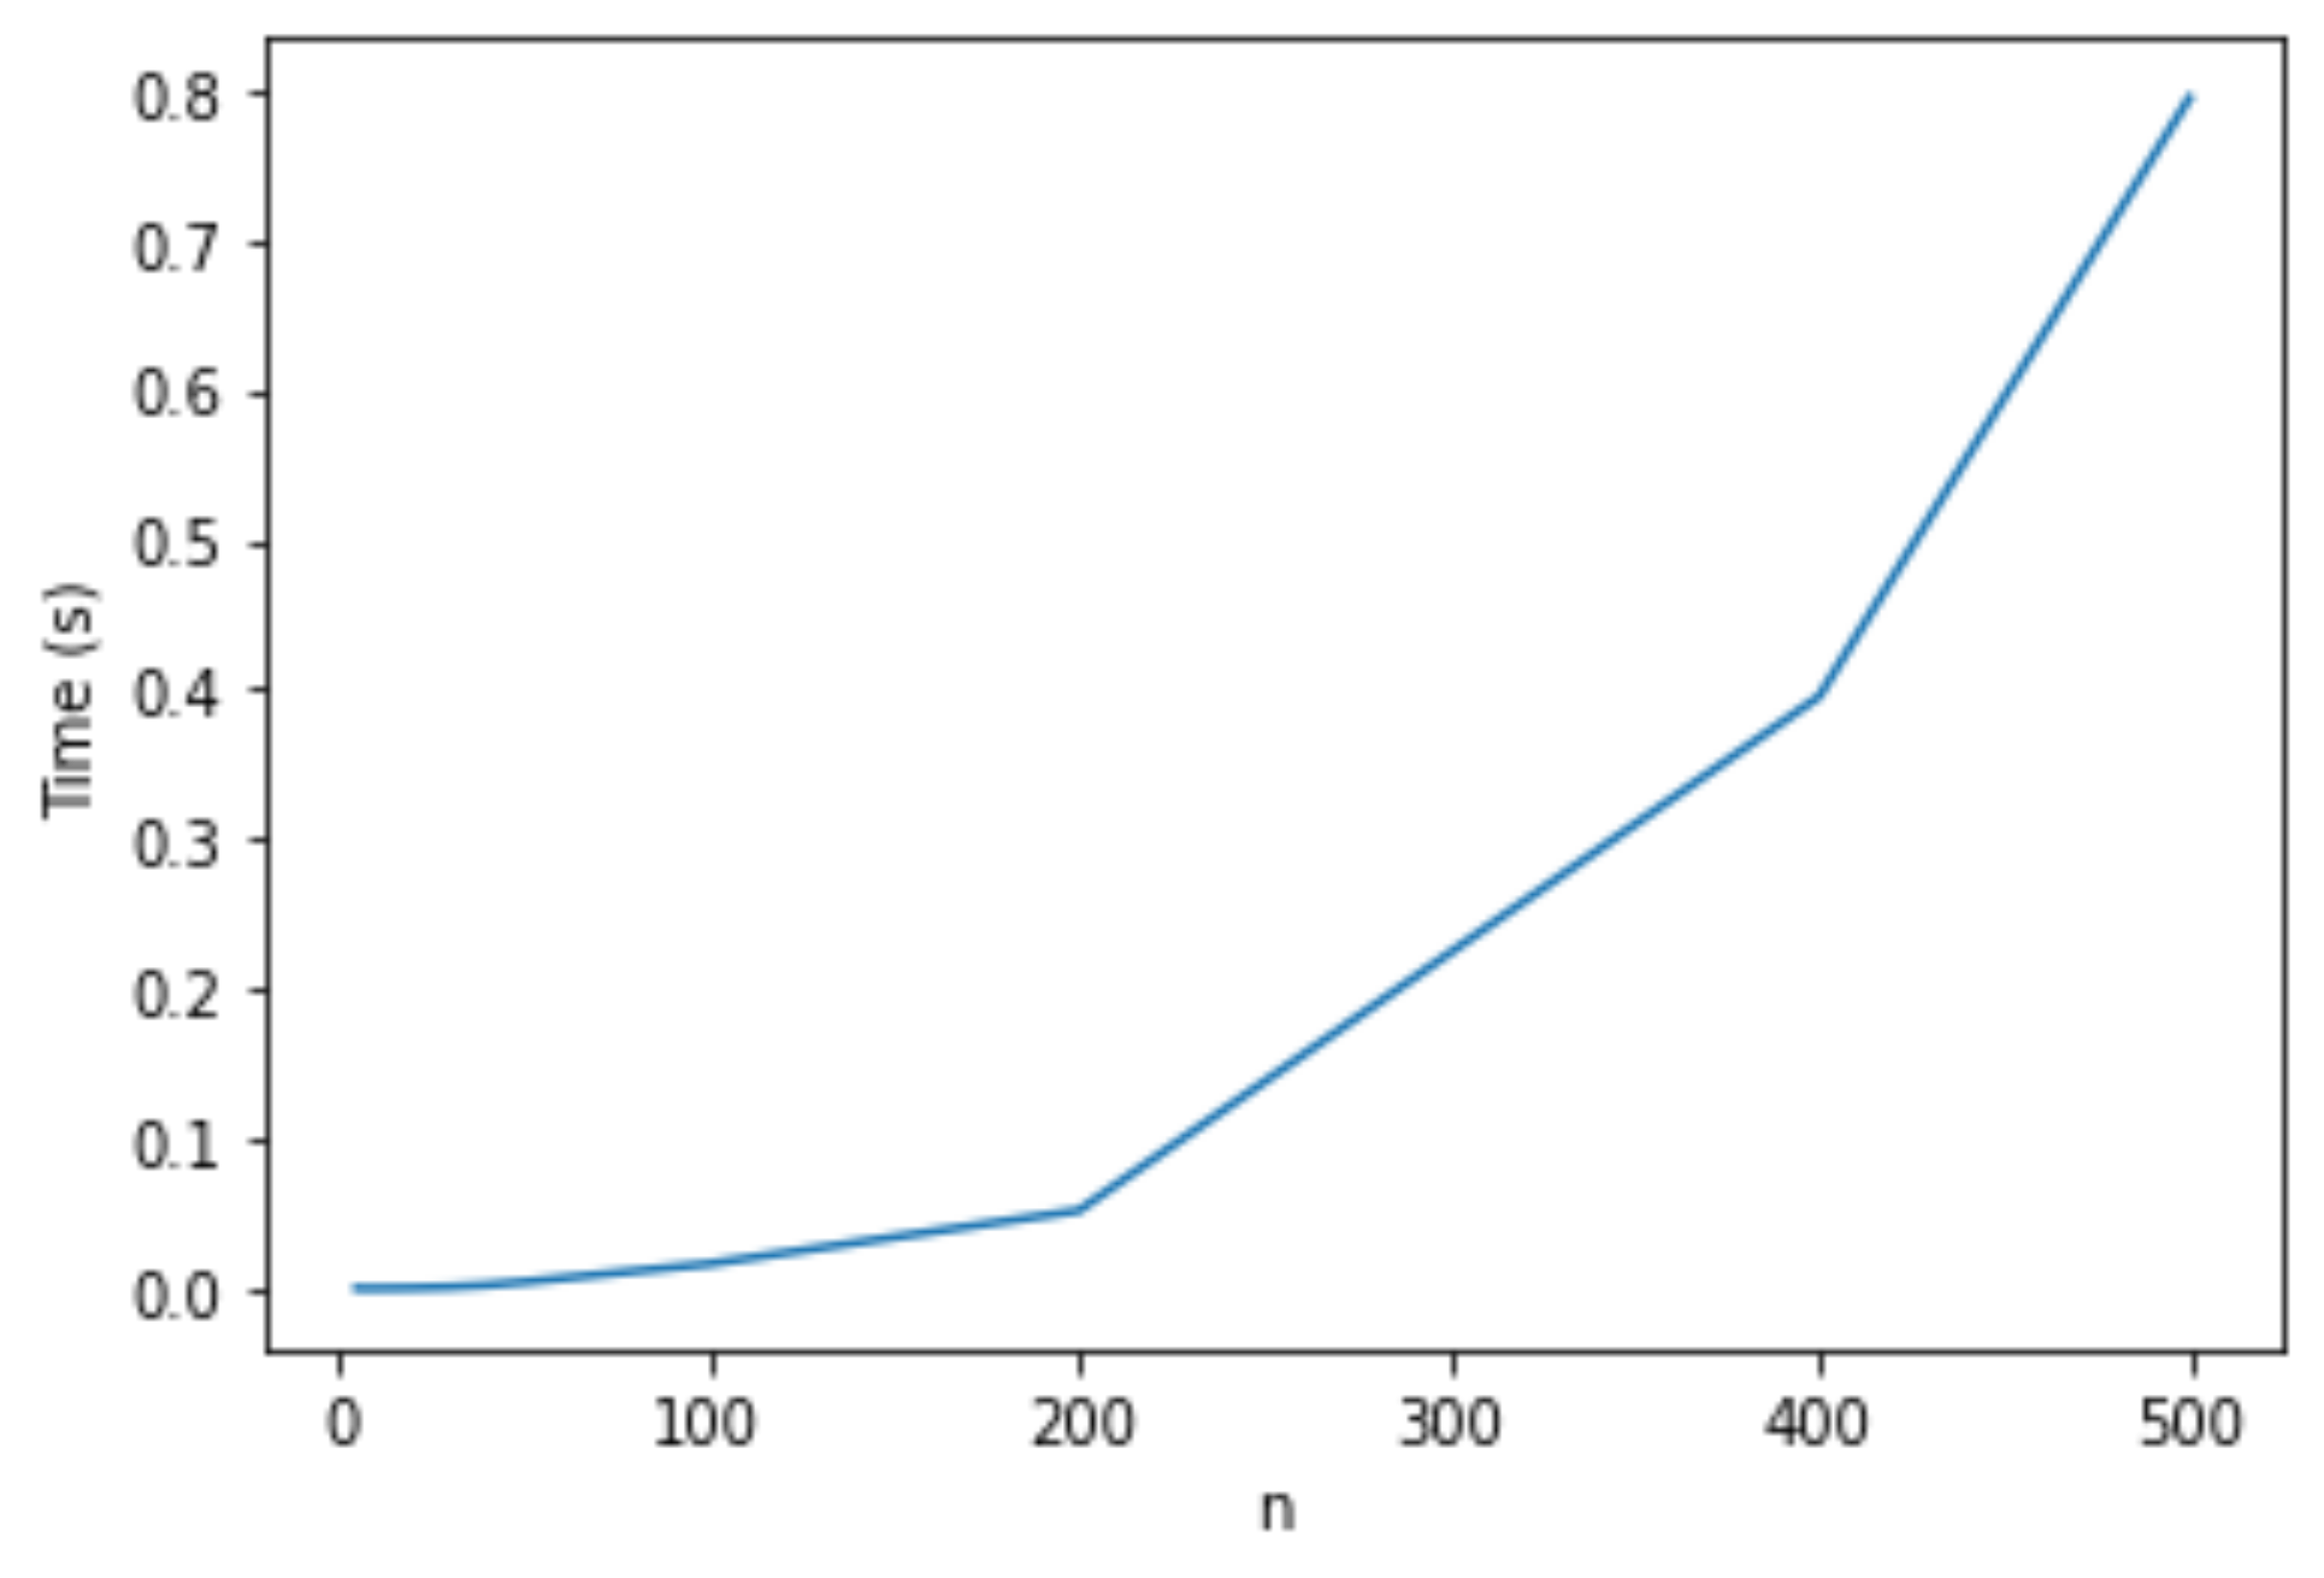
\includegraphics[width=1\linewidth]{figures/tempoTri.png}
					\end{center}
				\end{figure}
			\end{minipage}
			\hspace{0.1cm}
			\begin{minipage}{0.45 \linewidth}
				
				\begin{figure}[H]
					\begin{center}
						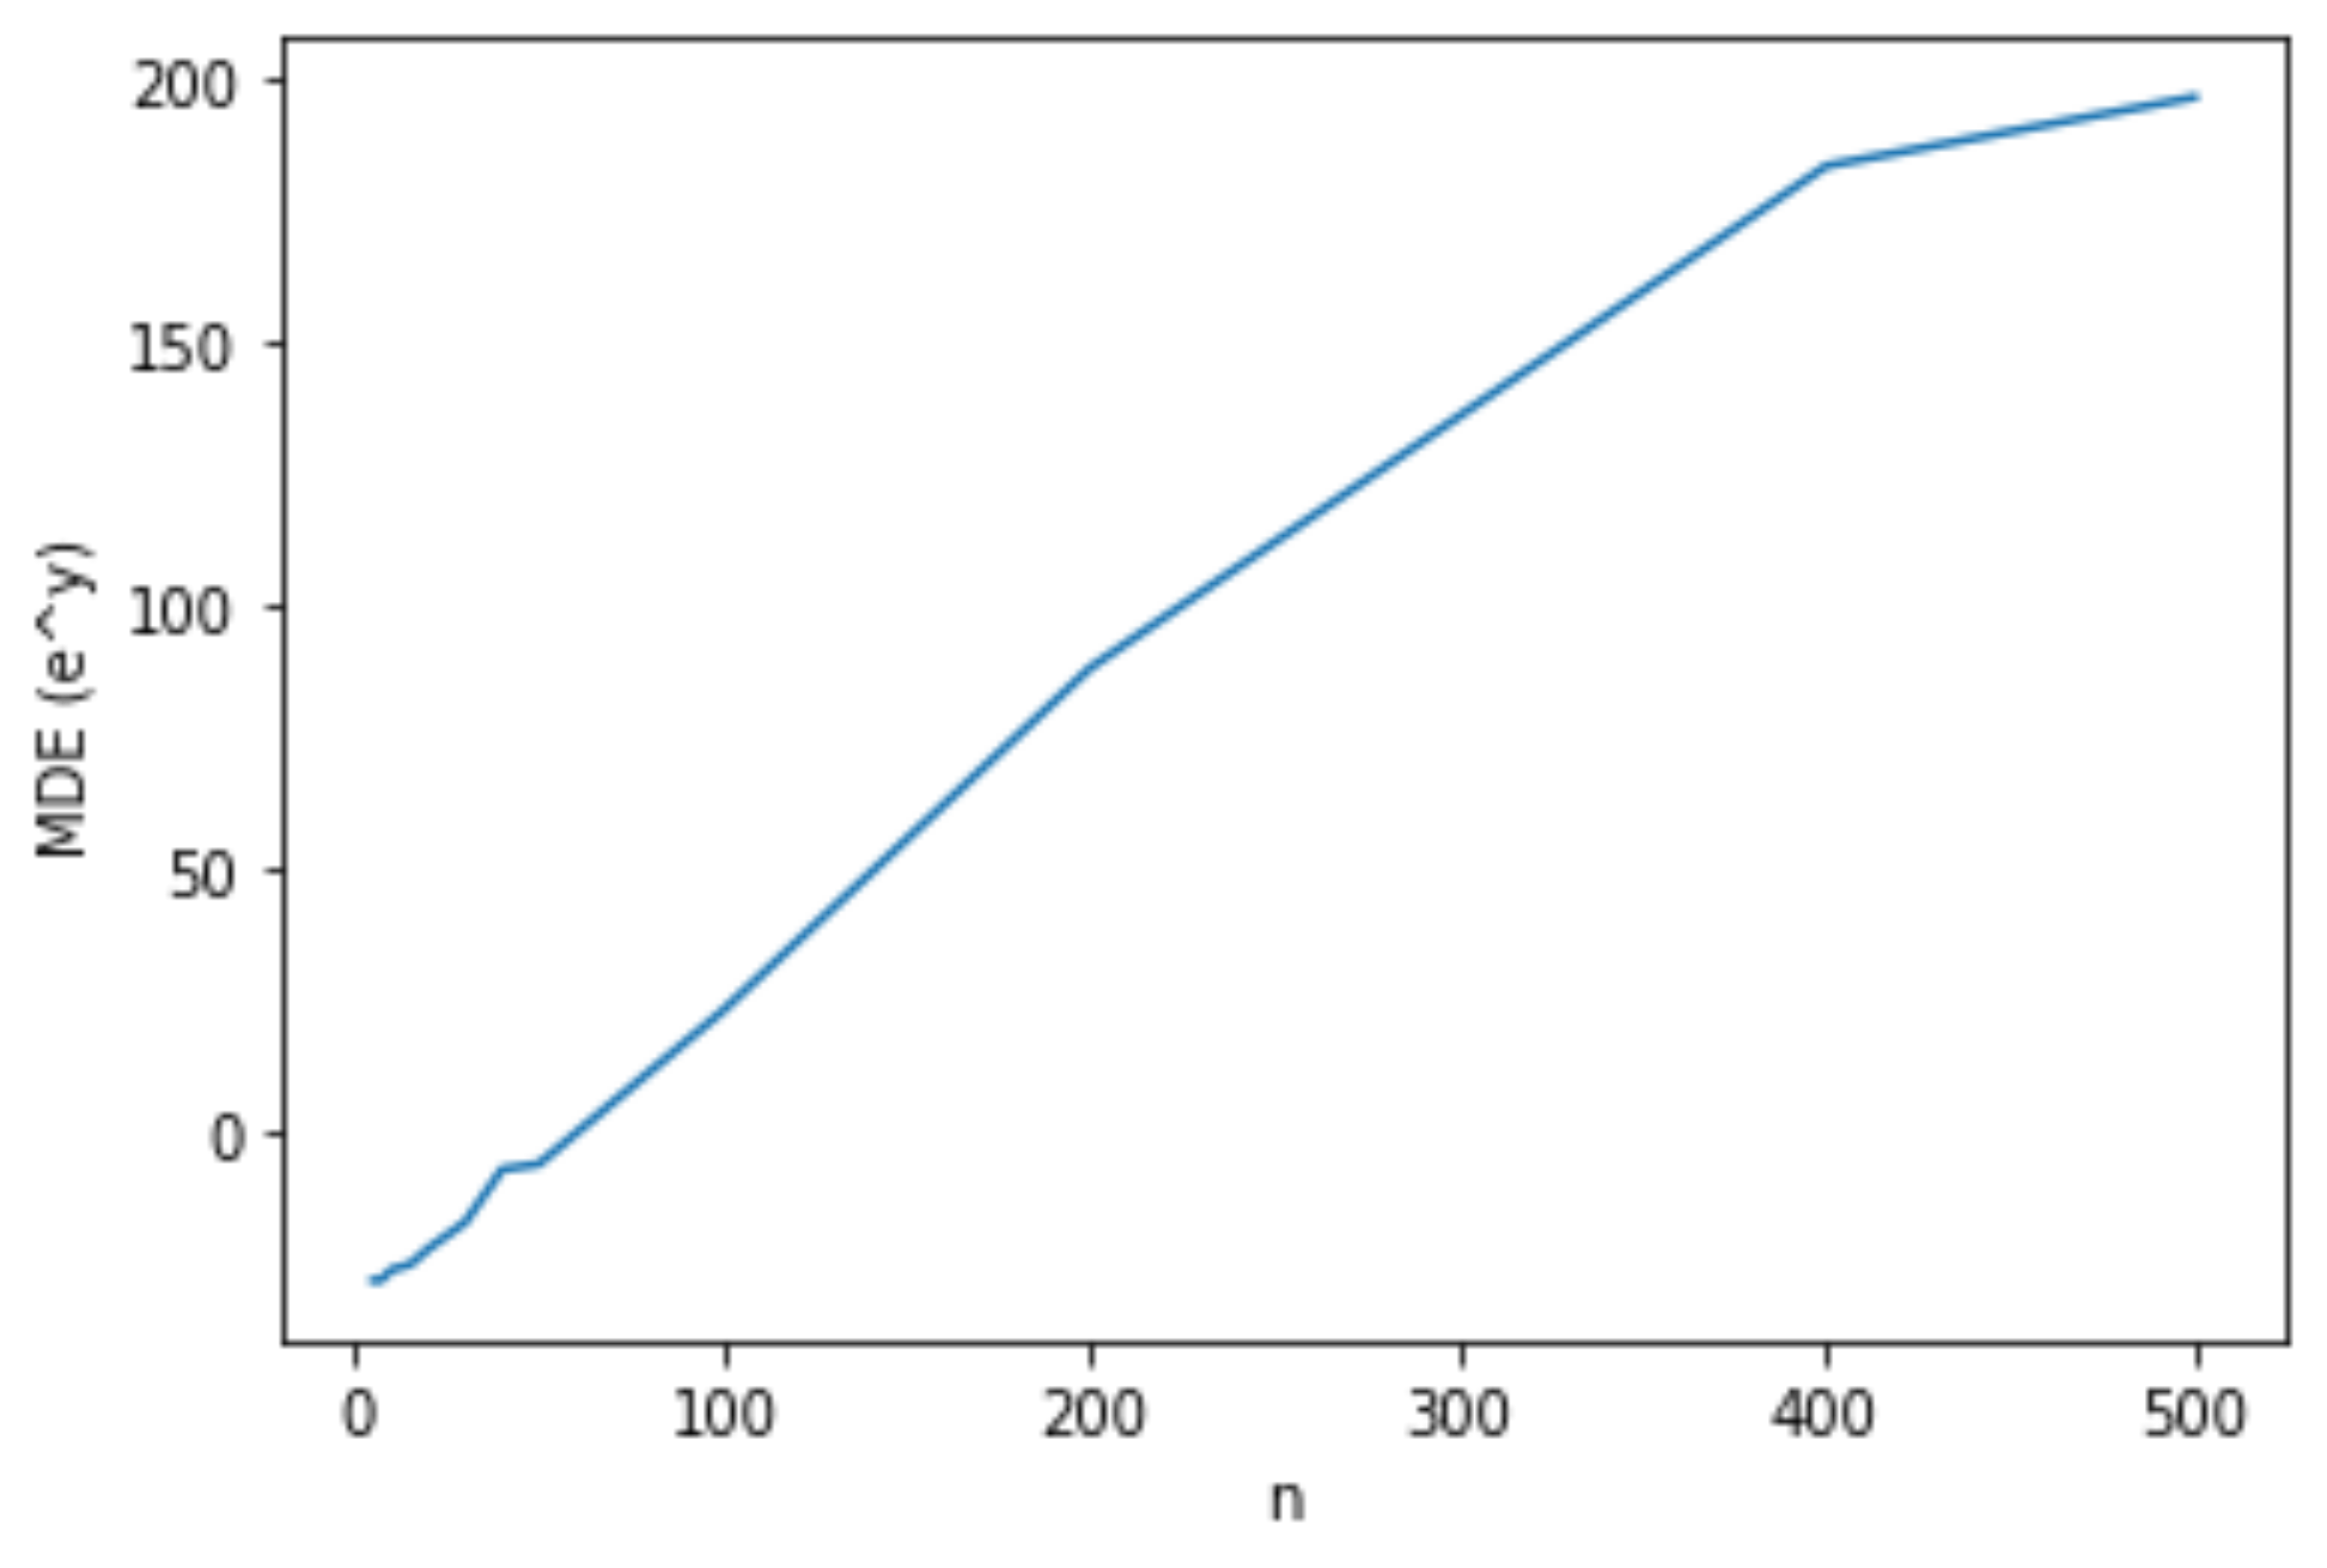
\includegraphics[width=1\linewidth]{figures/mdeTri.png}
					\end{center}
				\end{figure}
			\end{minipage}
		\end{center}
		\caption{A esquerda, o tempo de processo e, a direita, a ordem de grandeza associada ao MDE das soluções.}
		\label{fig:tri}
	\end{figure}
	
	Perceba o comportamento mostrado na Figura~\ref{fig:tri}. Teve-se que fazer uma linearização no gráfico que representa o MDE da solução, pois este cresceu exponencialmente e foi para a ordem de $10^{200}$ em 500 vértices. Esse comportamento se deu por conta dos erros acumulados entre as iterações.
	\\
	
	Uma proposta pensada para contornar essa situação infeliz foi alterar o valor de $\mathcal{P}$, deixando o menor, obrigando o algorítimo a calcular realizações utilizando vértices iniciais. Porém, isso implicaria em um grafo não completo, o que não condiz definição do Algorítimo~\ref{alg:realizacaoIterativa}.
	
	Outra solução proposta fora de utilizar sempre os primeiros vértices no lugar dos antecessores mais próximos. Isso significaria utilizar sempre os vértices âncoras para realizar os demais, semelhante com o que é feito no sistema GPS. Com isso, tivemos os resultados satisfatórios apresentados pela Figura~\ref{fig:triPri}. Perceba que mesmo com 500 vértices ainda obteve-se resultados com $MDE$ na ordem de $10^{-20}$.
	
	\begin{figure}[H]
		\begin{center}
			\begin{minipage}{0.45 \linewidth}
				\begin{figure}[H]
					\begin{center}
						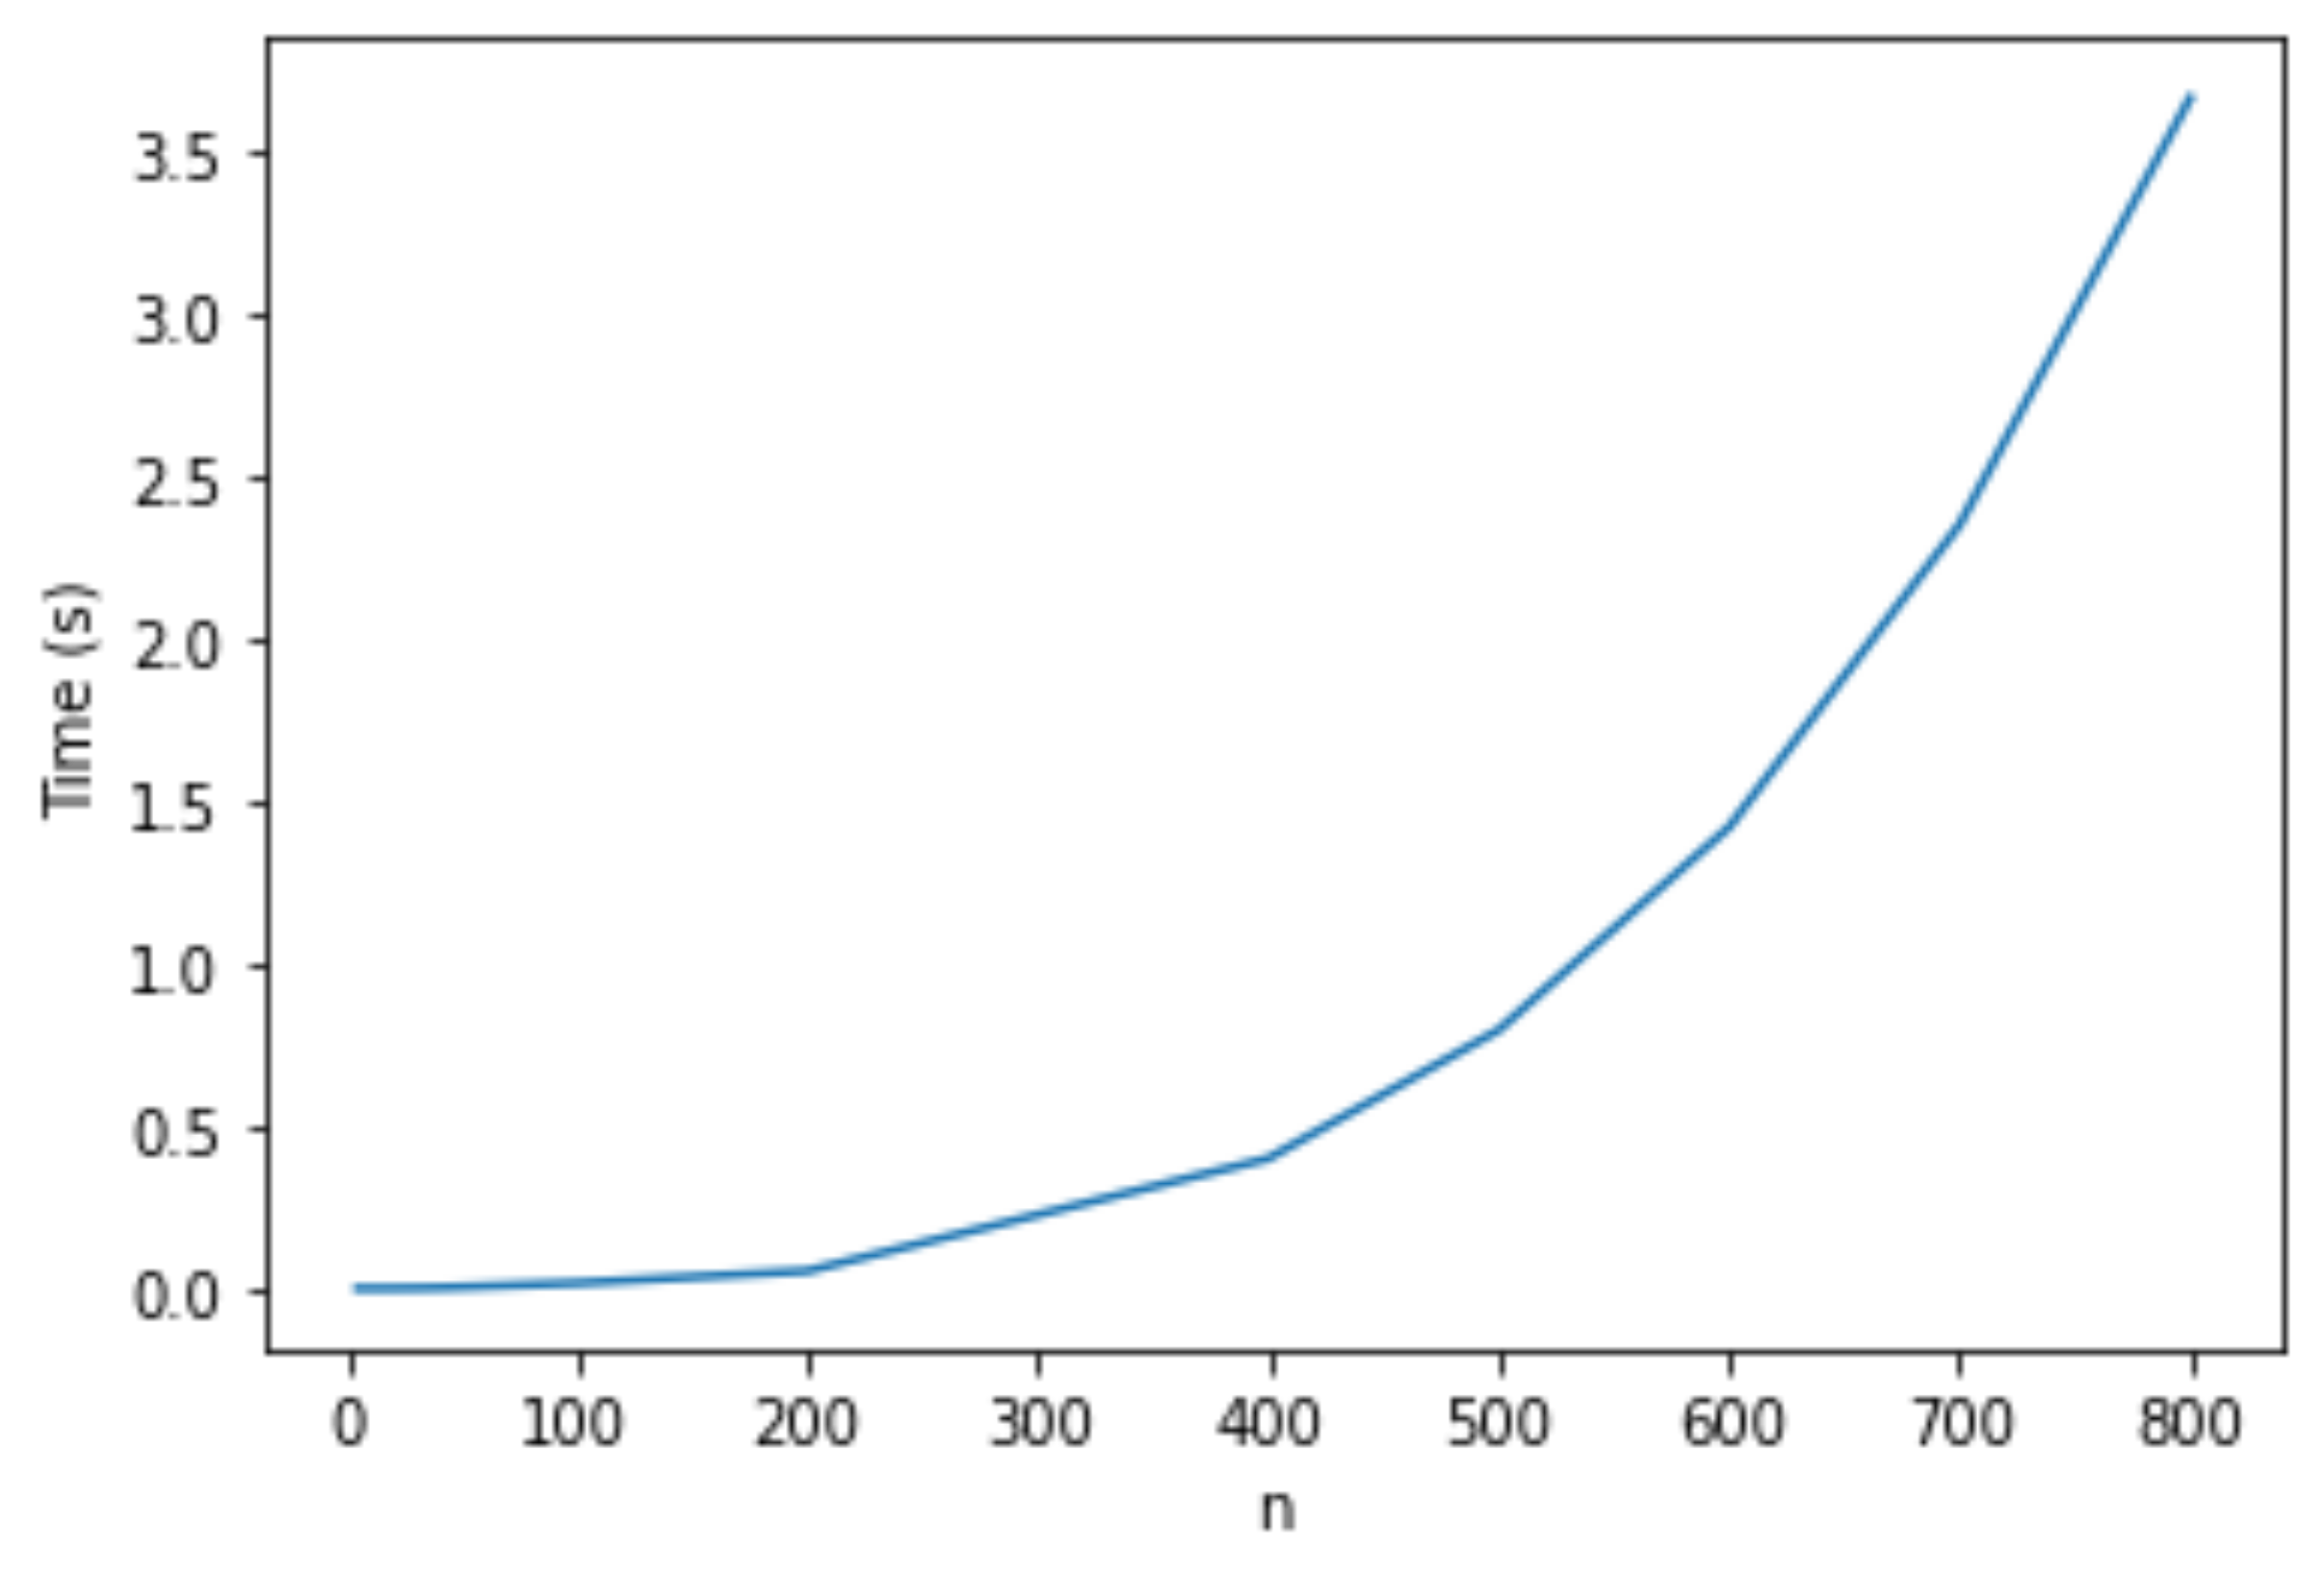
\includegraphics[width=1\linewidth]{figures/tempoTriPri.png}
					\end{center}
				\end{figure}
			\end{minipage}
			\hspace{0.1cm}
			\begin{minipage}{0.45 \linewidth}
				
				\begin{figure}[H]
					\begin{center}
						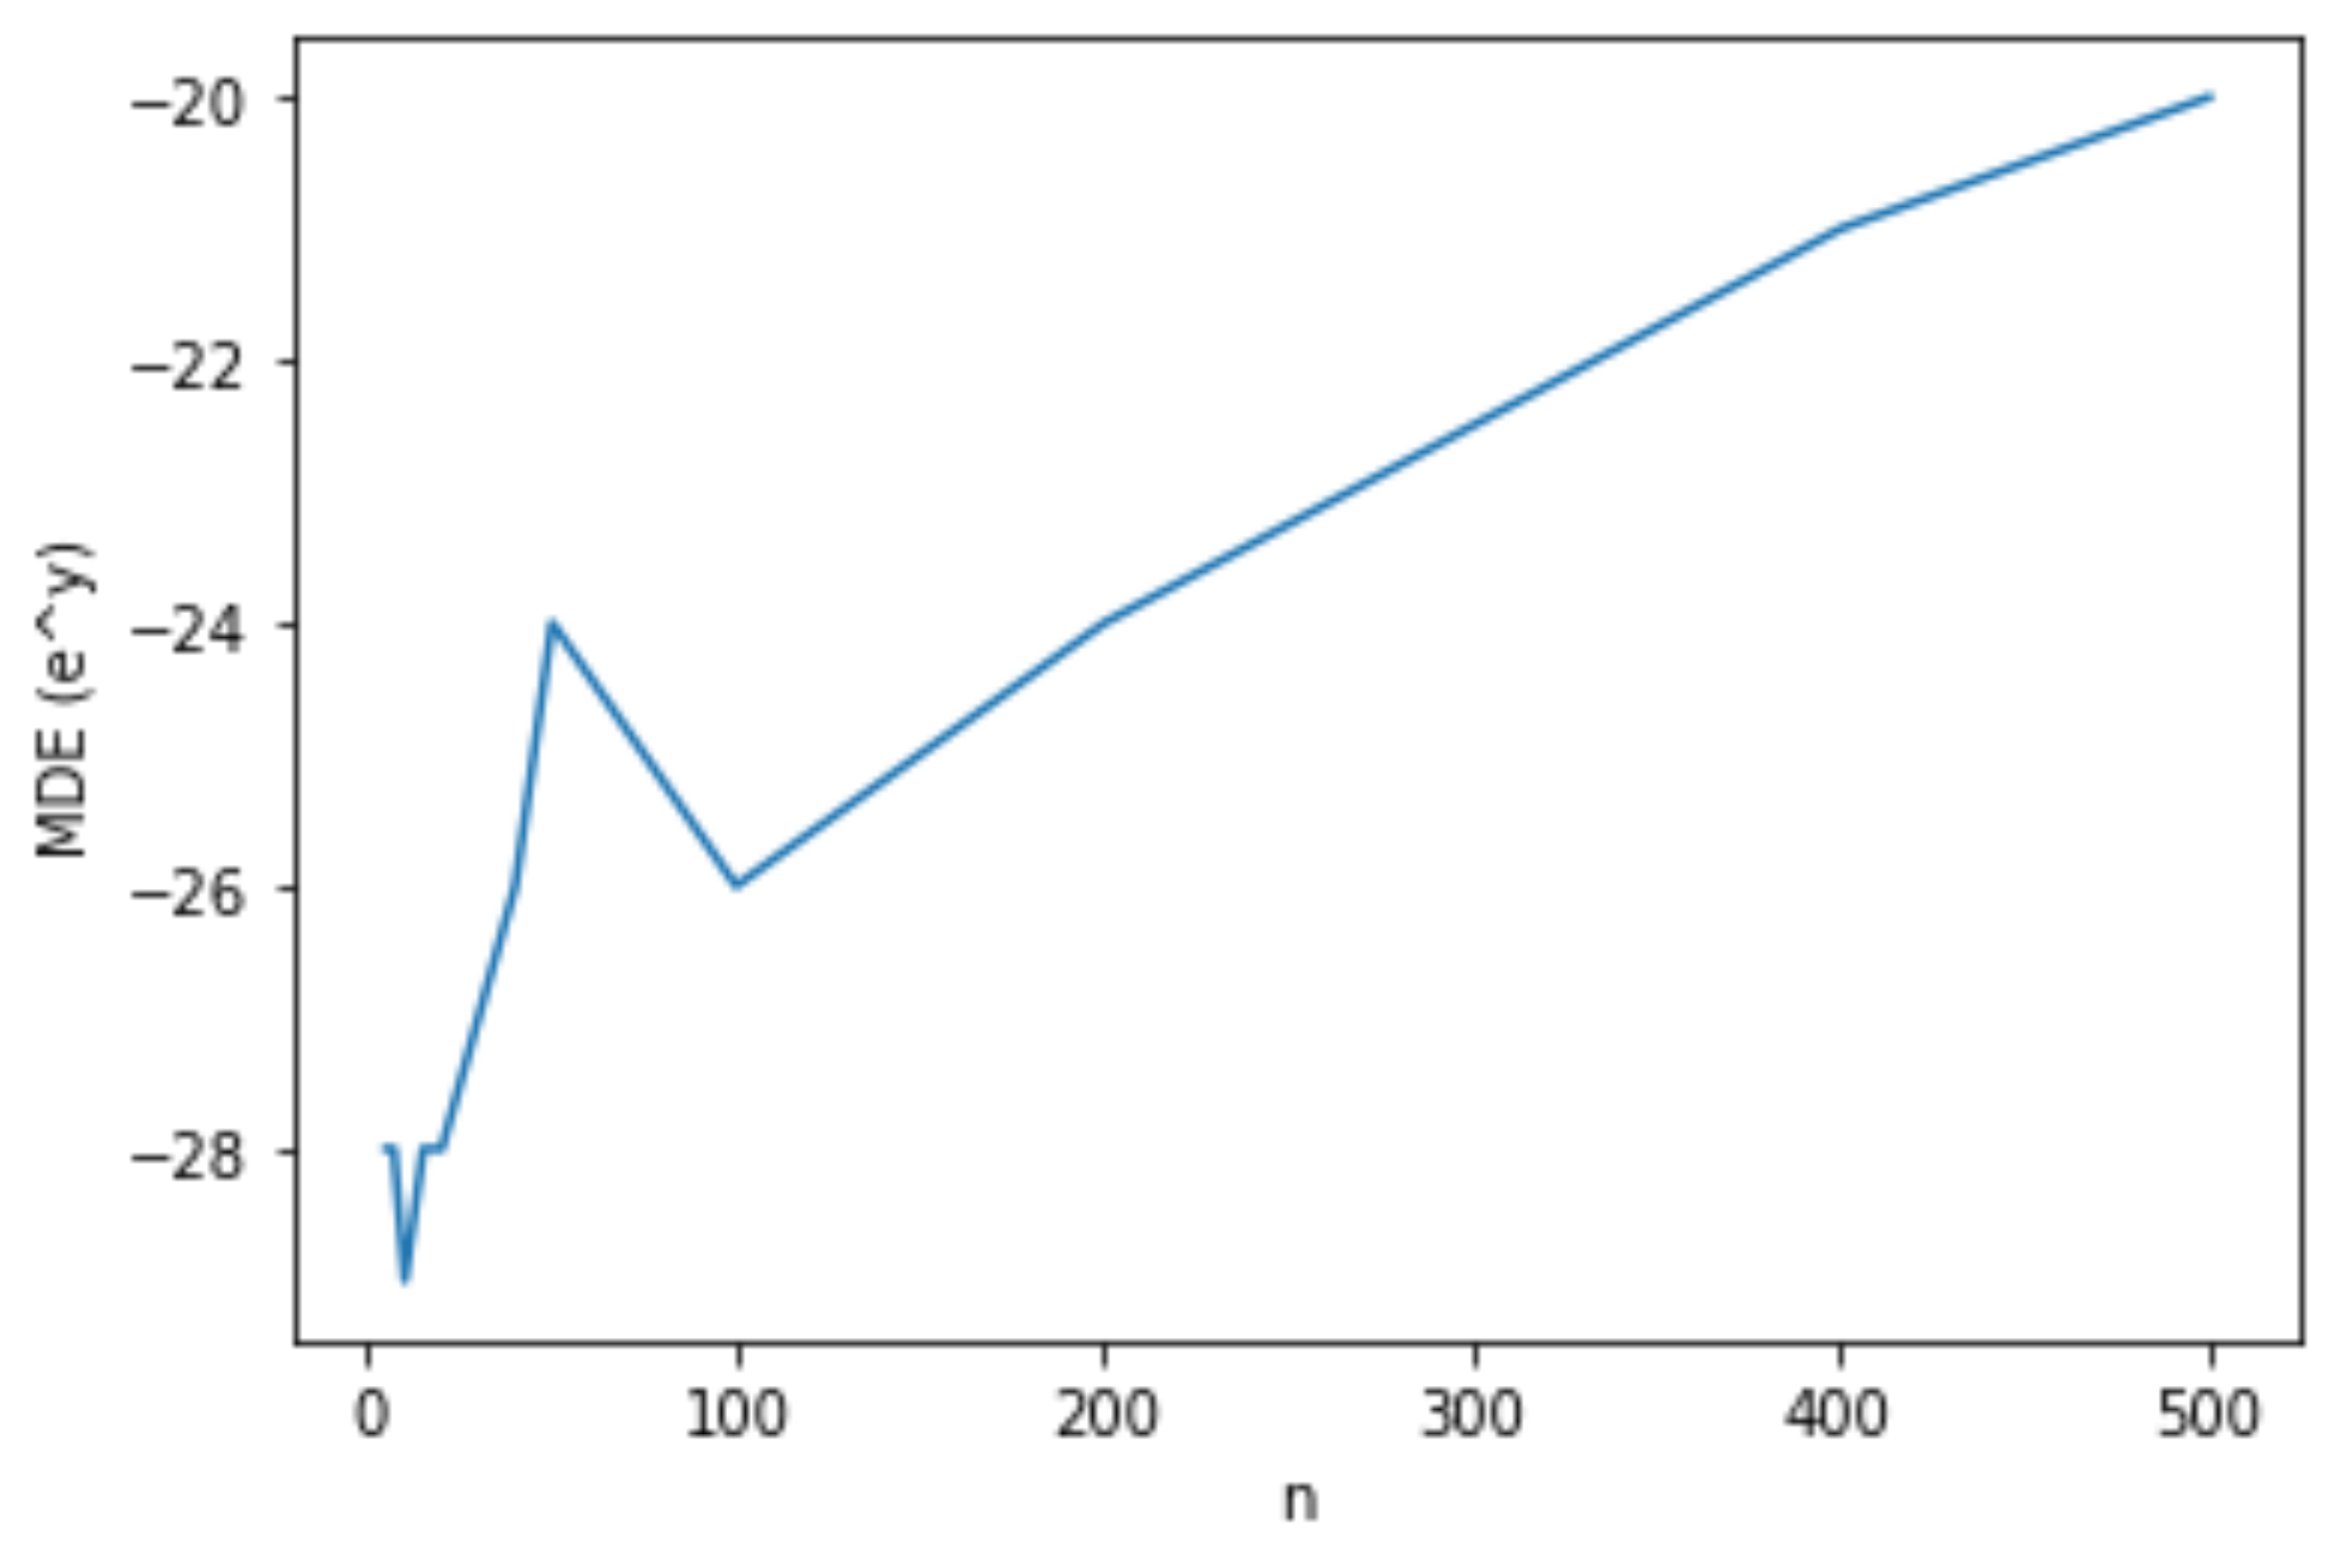
\includegraphics[width=1\linewidth]{figures/mdeTriPro.png}
					\end{center}
					\label{fig:mdeTri}
				\end{figure}
			\end{minipage}
		\end{center}
		\caption{A esquerda, o tempo de processo e, a direita, a ordem de grandeza associada ao MDE das soluções.}
		\label{fig:triPri}
	\end{figure}
	
	Também simulou-se o Algorítimo~\ref{alg:realizacaoTrilateration}, que teve um comportamento muito similar ao Algorítimo~\ref{alg:realizacaoIterativa}, como era de se esperar. Também usou-se instâncias $n$ variando em $\{5, 6, 7,10,15,20,30,40,50,100,200,400,500\}$. Porém, agora, com uma busca inteligente por vértices adjacentes, pode-se variar $\mathcal{P}$ afim de analisar diferentes geometrias para o problema, como apresenta-se a seguir.
	
	\subsubsection*{Instâncias com 70\% de arestas}
	
	\begin{figure}[H]
		\begin{center}
			\begin{minipage}{0.45 \linewidth}
				\begin{figure}[H]
					\begin{center}
						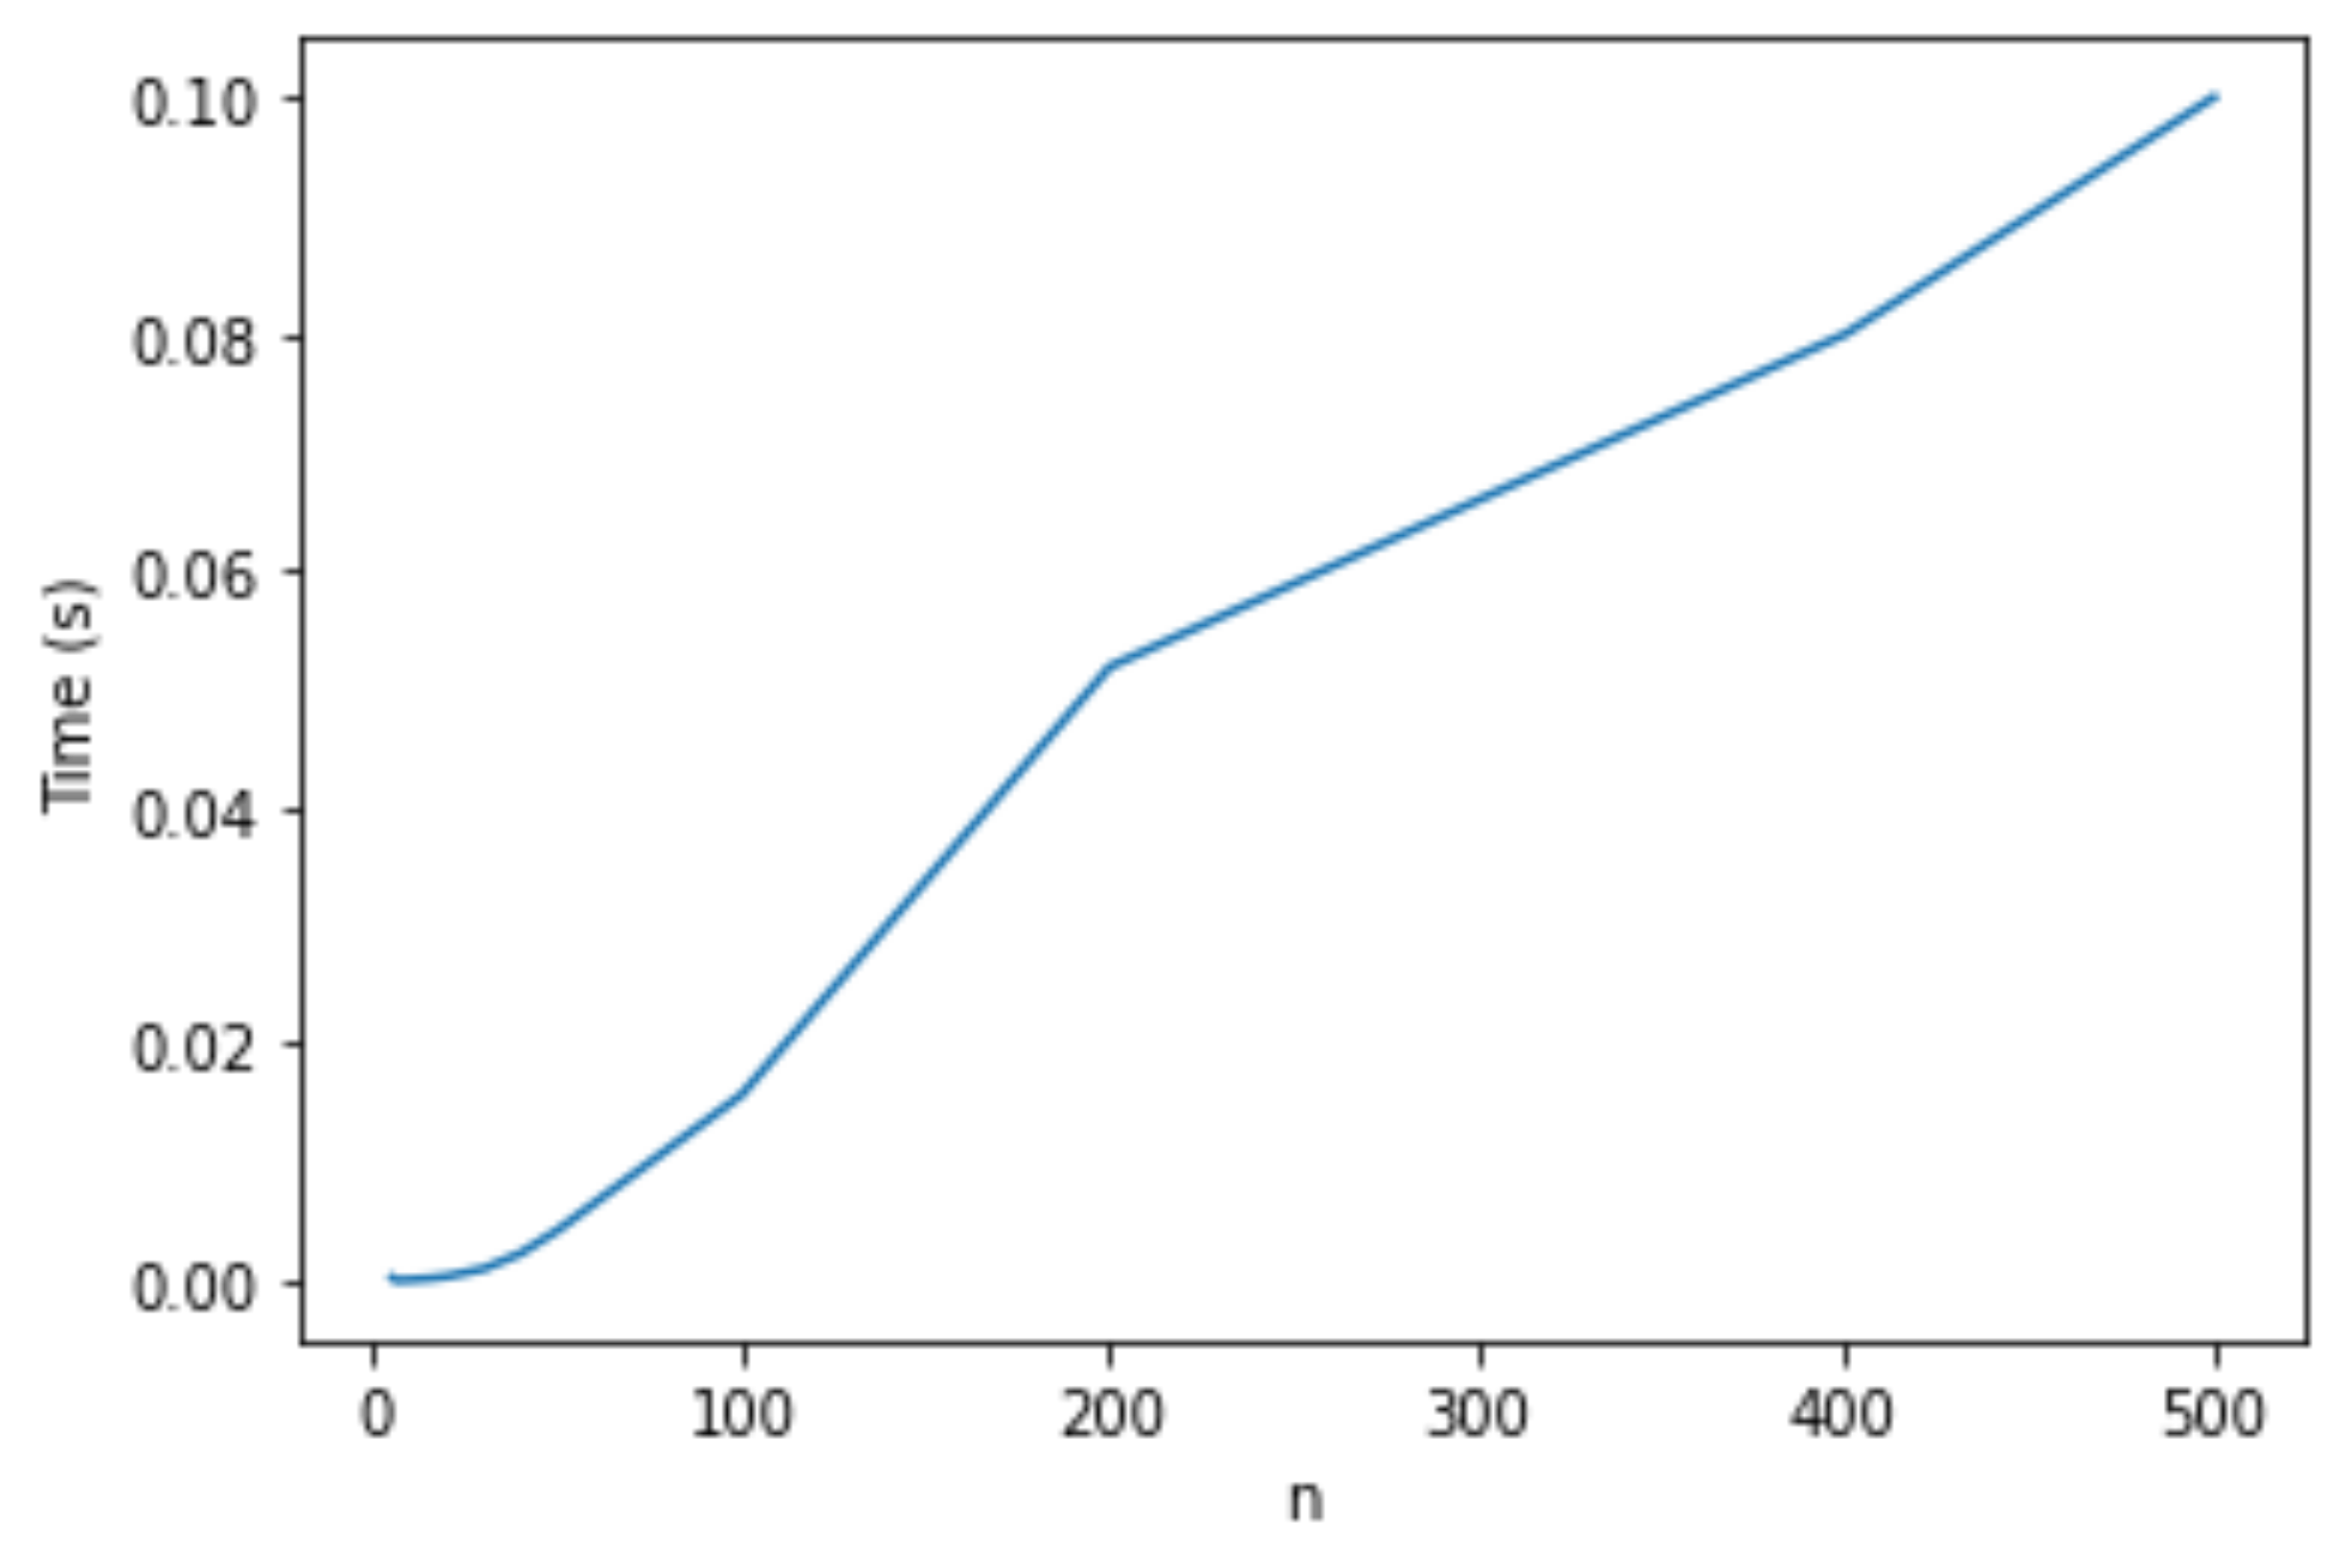
\includegraphics[width=1\linewidth]{figures/timeTriPro1.png}
					\end{center}
				\end{figure}
			\end{minipage}
			\hspace{0.1cm}
			\begin{minipage}{0.45 \linewidth}
				
				\begin{figure}[H]
					\begin{center}
						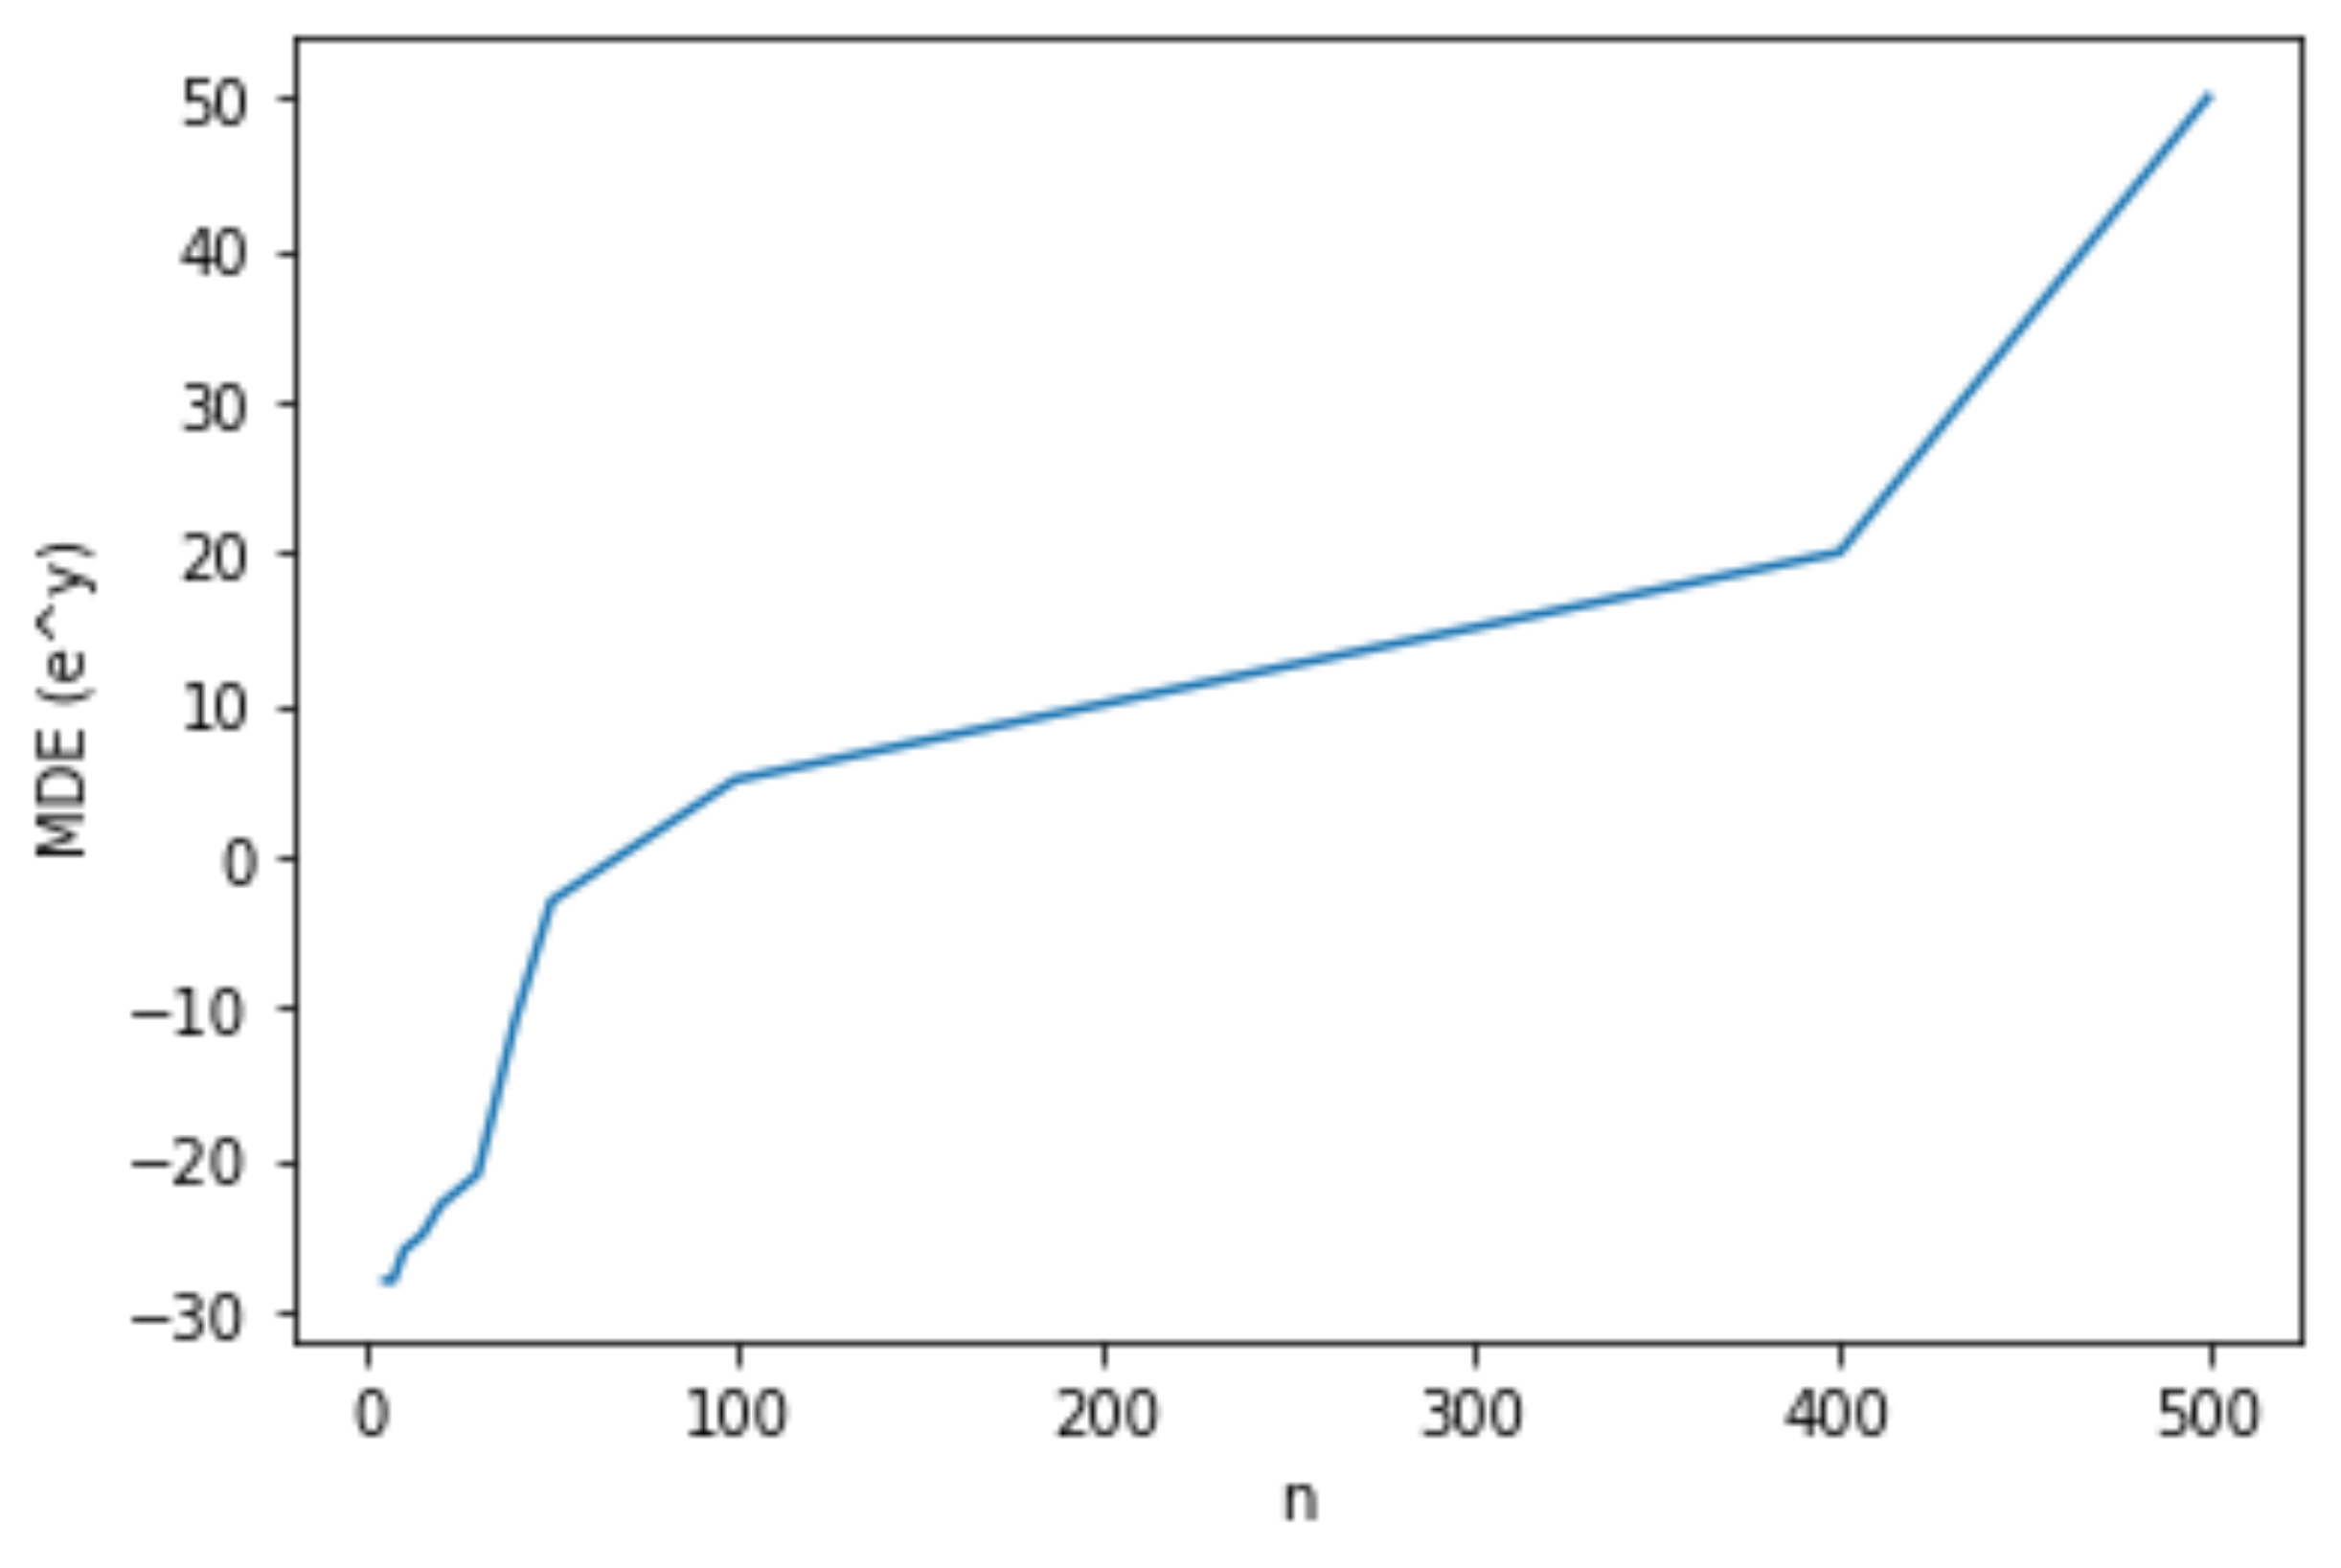
\includegraphics[width=1\linewidth]{figures/mdeTriPro1.png}
					\end{center}
					\label{fig:mdeTri}
				\end{figure}
			\end{minipage}
		\end{center}
		\caption{A esquerda, o tempo de processo e, a direita, a ordem de grandeza associada ao MDE das soluções. Utilizou-se $\mathcal{P} = 0.7$.}
		\label{fig:triPri4}
	\end{figure}
	
	\subsubsection*{Instâncias com 5\% de arestas}
	
	\begin{figure}[H]
		\begin{center}
			\begin{minipage}{0.45 \linewidth}
				\begin{figure}[H]
					\begin{center}
						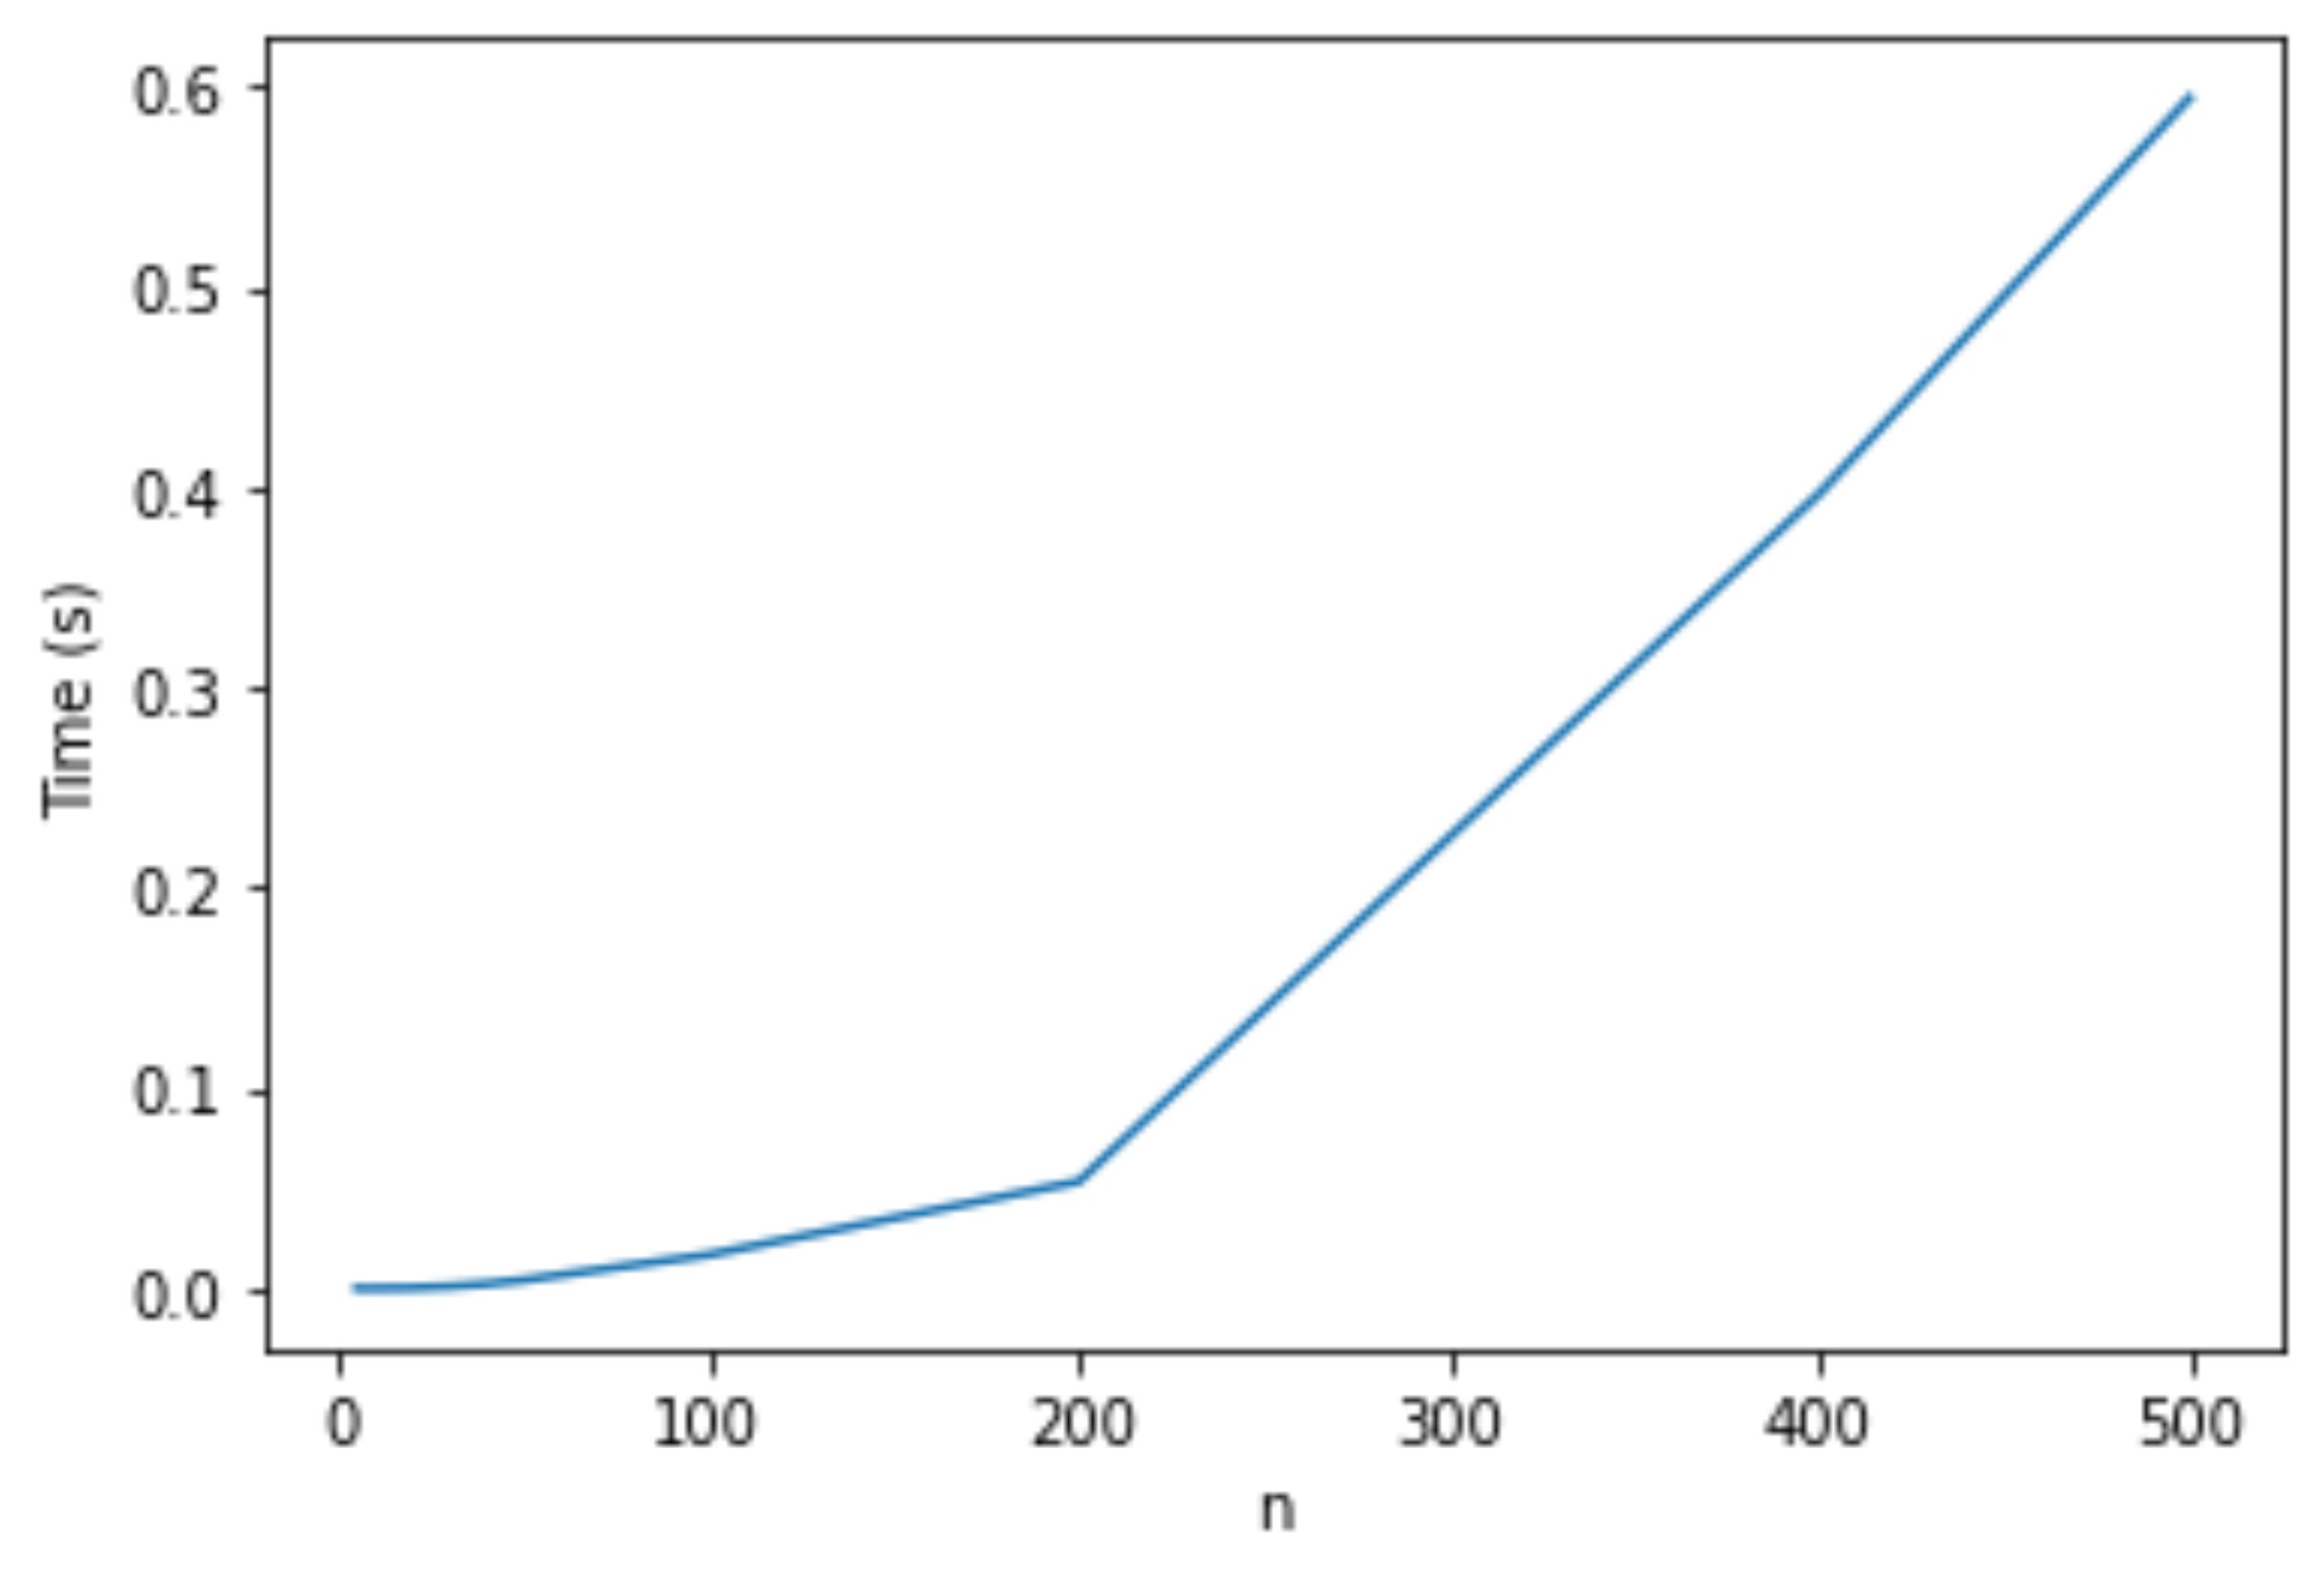
\includegraphics[width=1\linewidth]{figures/timePro2.png}
					\end{center}
				\end{figure}
			\end{minipage}
			\hspace{0.1cm}
			\begin{minipage}{0.45 \linewidth}
				
				\begin{figure}[H]
					\begin{center}
						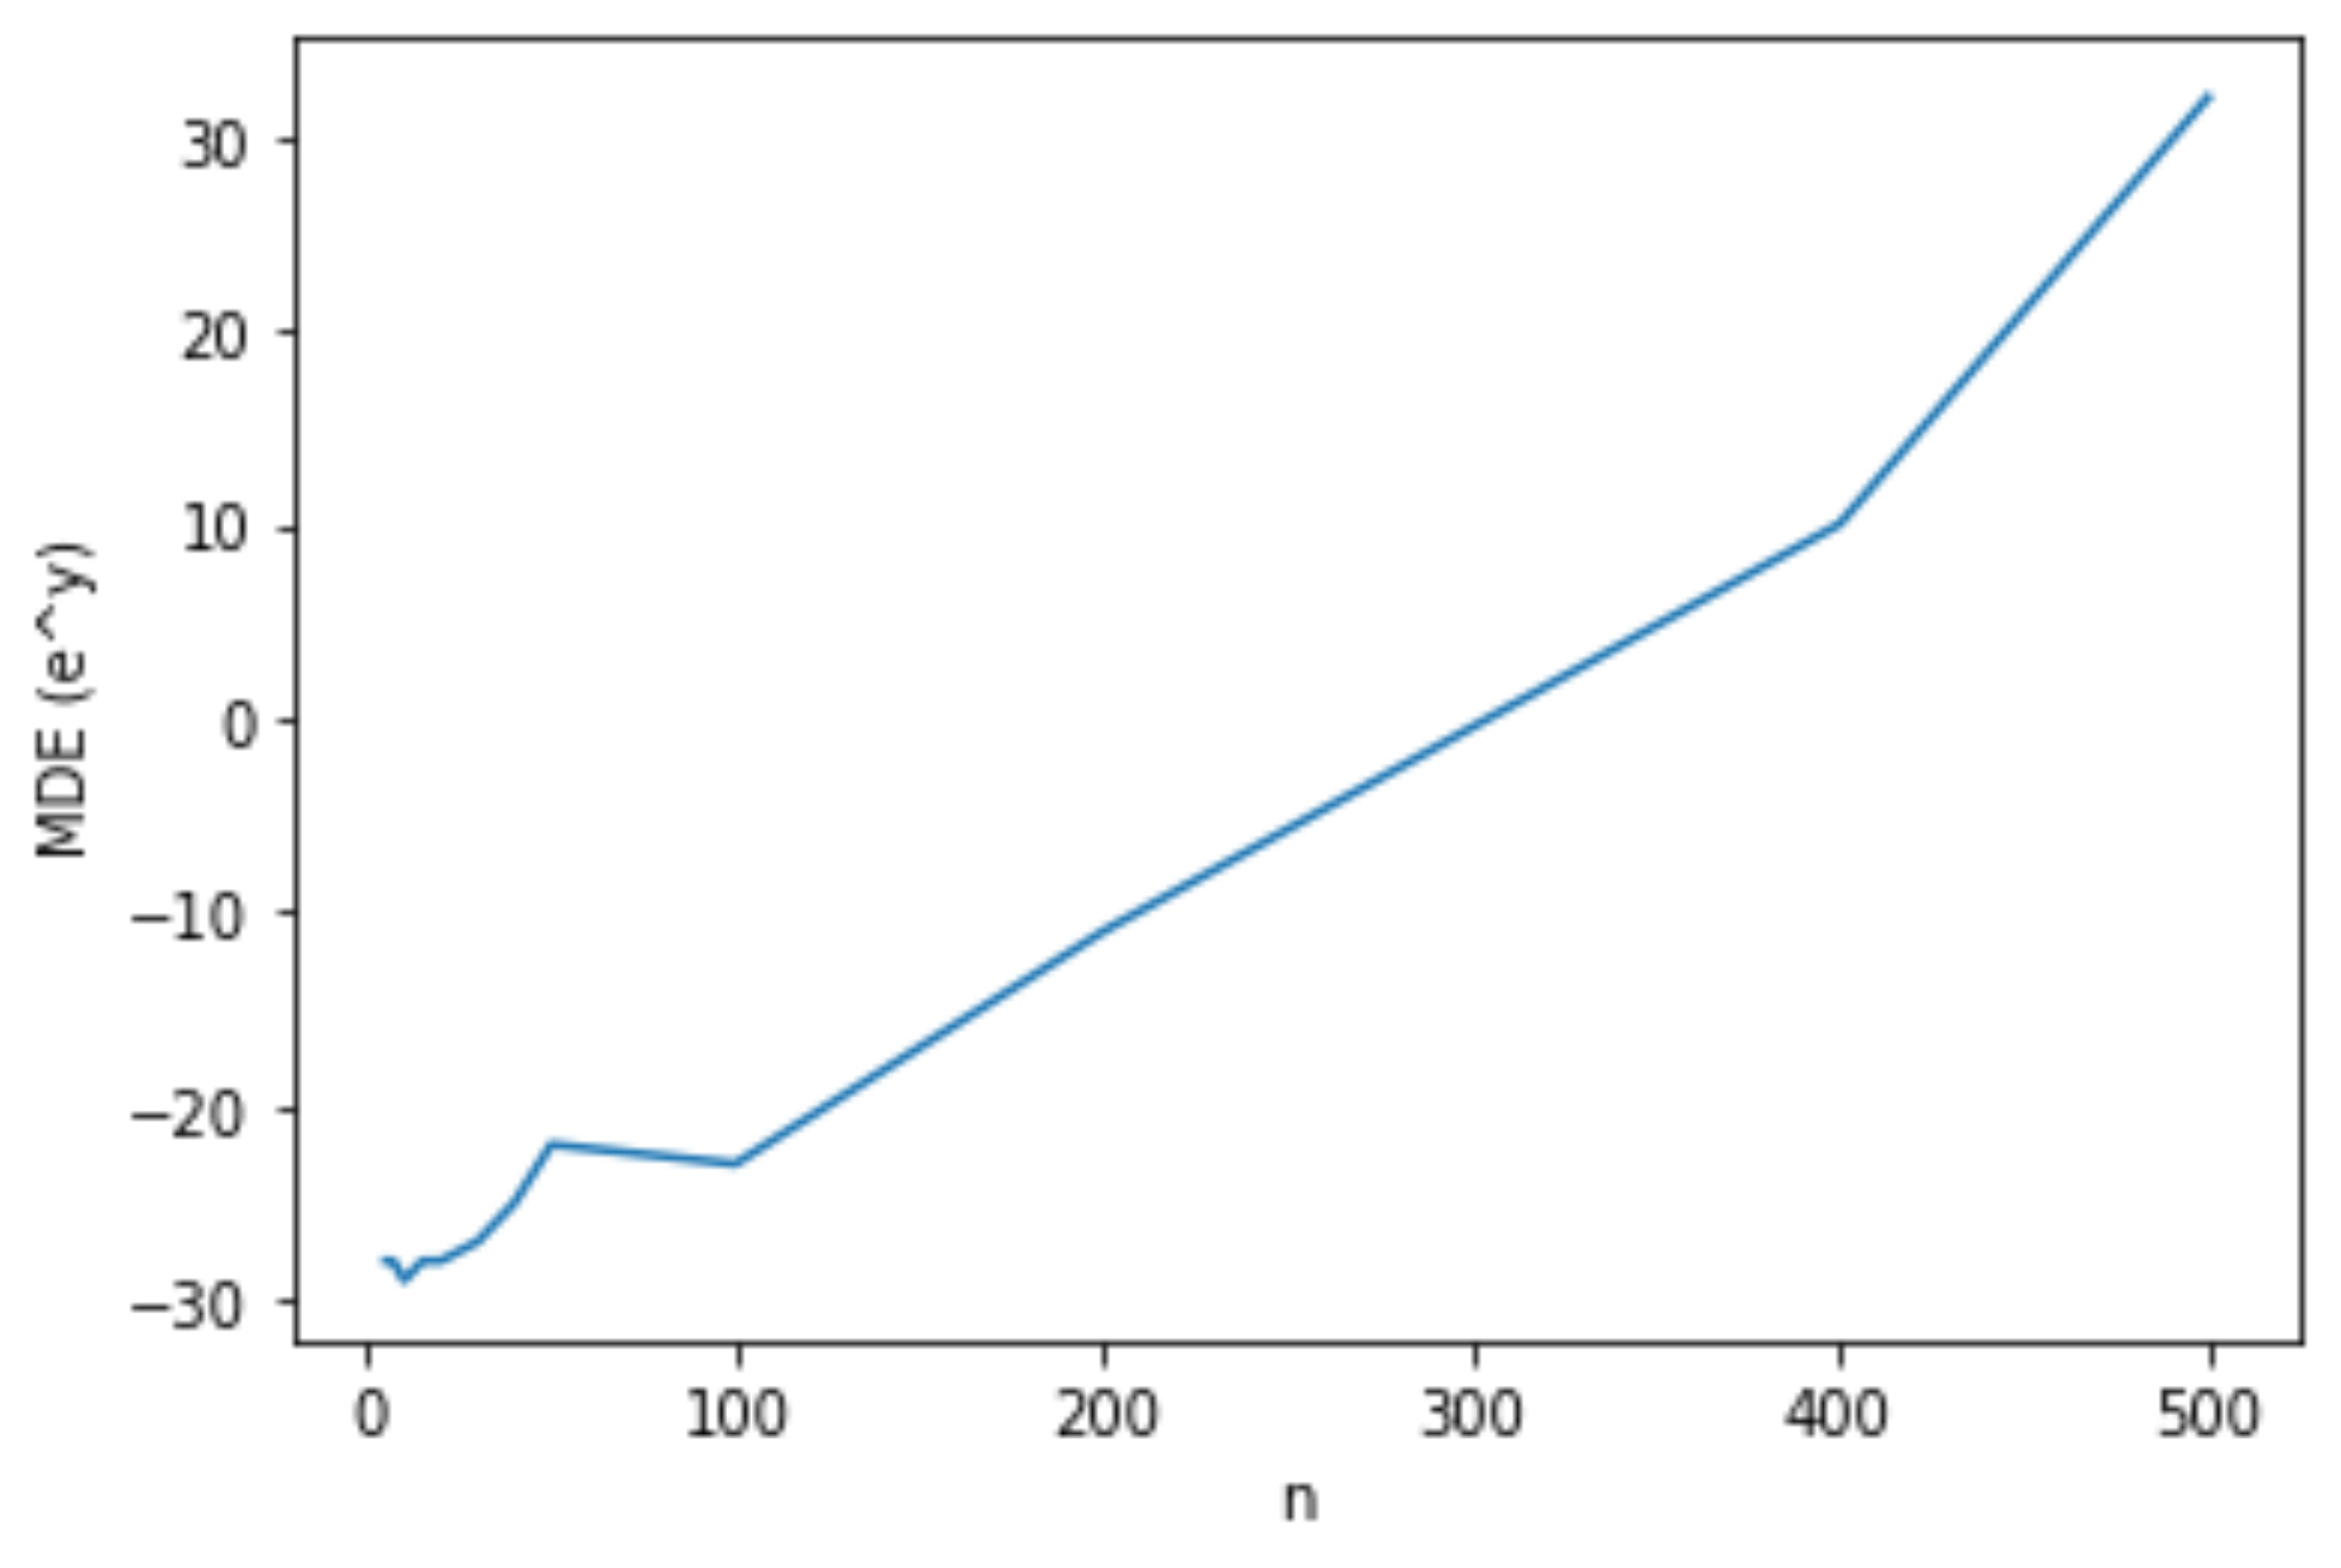
\includegraphics[width=1\linewidth]{figures/mdeTriPro2.png}
					\end{center}
					\label{fig:mdeTri}
				\end{figure}
			\end{minipage}
		\end{center}
		\caption{A esquerda, o tempo de processo e, a direita, a ordem de grandeza associada ao MDE das soluções. Utilizou-se $\mathcal{P} = 0.05$.}
		\label{fig:triPri3}
	\end{figure}
	
	Como esperado, é perceptível uma grande melhora na MDE das soluções conforme se diminui o valor de $\mathcal{P}$. 
	
	Também deve-se perceber que o tempo não obedeceu um padrão perfeito. Podemos relacionar esse fato com a aleatoriedade das instâncias, como pode-se notar que o Algoritmo~\ref{alg:realizacaoTrilateration} teve maios volatilidade no padrão temporal. Mesmo assim, há um consenso. As soluções mostradas nas Figuras~\ref{fig:triPri} e~\ref{fig:triPri3}, por exemplo, demonstram claramente um padrão polinomial, indo de encontro com o que foi apresentado na seção~\ref{sec:oi}.
	
	\newpage
	\section{Considerações Finais}
	Com isso, concluí-se o estudo sobre a Geometria de Distâncias aplicada ao problema de localização de sensores, tal qual teve como resultado um algorítimo que garante encontrar a solução do problema (se houver). .
	\\
	
	Nos cabe, nesse momento, voltarmos atenção às propostas levantadas internamente no início do projeto e verificar se elas foram cumpridas. Seguem o conjunto de objetivos específicos desse projeto, munidos de breve conclusão:
	
	\begin{enumerate}
		
		\item Estudar formas viáveis (pelos vieses energético, de construção e precisão da medida) para obtenção das distâncias entre os elementos do sistema físico:
		
		Fortemente embasado em \cite{savvides2001dynamic} e \cite{sensorsForMobileRobots}, faz-se uma apresentação sobre esses conceitos na Seção~\ref{sec:sensores}. 
		
		\item Estudar as possíveis distribuições dos Robôs Móveis em um sistema genérico, visando verificar quais conjuntos de dados possam ser garantidos como entradas para a construção do problema:
		
		Além de estudar distribuições genéricas, como em \cite{eren2004rigidity}, desenvolve-se na Seção~\ref{sec:disc} o Algorítimo~\ref{alg:instancia}, que cria instâncias aleatórias com diferentes densidades de ligações.
		
		\item Verificar a solução do Discretizable Order Problem \cite{carlileGDandAplications} aplicado ao problema proposto e estudar o ordenamento de vértices que se adeque aos objetivos do trabalho:
		
		Durante o desenvolvimento da Seção~\ref{sec:GD}, percebeu-se que uma ordem de discretização não seria necessária, visto que a definição do problema necessita de uma única solução \cite{libertiEDG}. Por conta disso, definiu-se a ordem de $K$-lateração, que garante a unicidade de solução.
		
		\item Caso consiga-se uma boa ordenação para os vértices, verificar a aplicação do algorítimo Branch-And-Prune \cite{carlile:BP} para a solução do problema proposto. Se não for possível, estudar outros algorítimos que possam solucionar o problema:
		
		Visto que o problema não era discreto, não fora possível aplicar o algorítimo Branch-And-Prune. Ao invés disso, se propôs o Algorítimo~\ref{alg:realizacaoTrilateration}, que utiliza a trilateração como núcleo e garante no máximo uma solução.
		
		\item Estudar a complexidade computacional do algorítimo proposto aplicado as possíveis distribuições:
		
		Isso foi feito no fim das Seções~\ref{sec:GD} e~\ref{sec:disc}, onde verificou-se que o algorítimo pode ser resolvido em tempo polinomial. Também mostrou-se um estudo sobre diferentes visões da geometria do problema afim de minimizar os erros associados. 
		
		\item Simular computacionalmente o algoritmo para solução do problema com instâncias artificialmente geradas, dominando cada passo utilizado:
		
		Simulações apresentadas, de forma satisfatória, na Seção~\ref{sec:disc}.
		
		\item Aplicar o algoritmo estudado em estruturas de pequena escala, como instâncias reais do problema:
		
		Não fora possível cumprir este último objetivo. Infelizmente, a manufatura de robôs móveis usando sensores de distância se demonstrou excessivamente custosa \cite{savvides2001dynamic, sensorsForMobileRobots}.
		
		Vale lembrar, porém, que a utilização de instâncias artificiais genéricas se mostrou de grande importância. Pode-se averiguar e discutir sobre diferentes geometrias, mesmo sem a prototipação de fato.
		
	\end{enumerate}
	
	Como experiências futuras, deseja-se estudar mais sobre a obtenção e tratamento de dados de distâncias, visto que esses possuem erros de medida \cite{sensorsForMobileRobots} (não levados em consideração nesse trabalho). Alguns trabalhos relacionados à Geometria de Distâncias aplicada ao caso intervalar são mostrados em \cite{wsnlSemidefinitePrograming}. Há curiosidade em ver como medida MDE se comporta para uma quantidade grande de vértices associados a erros de medida.
	
	Também deseja-se fazer estudos sobre geometrias mínimas para o problema, como feito em \cite{wsnlFewAnchors}. Deseja-se verificar um conjunto de condições que restringem o movimento de um robô móvel afim de garantir que este ainda possa ser localizado.
	
	\newpage
	\phantomsection
	\addcontentsline{toc}{section}{Referências}
	
	\bibliographystyle{unsrt}
	\bibliography{references}
	
	\newpage
	\appendix
	\input{secGD/apendices.tex}

\end{document}

	
	\newpage
	
	 \documentclass[a4paper,12pt]{article}
\usepackage[a4paper,top=3cm,bottom=2cm,left=3cm,right=3cm,marginparwidth=1.75cm]{geometry}
\usepackage[brazil]{babel}
\usepackage[T1]{fontenc}
\usepackage[utf8]{inputenc}
\usepackage{amsmath}
\usepackage{MnSymbol}
\usepackage{wasysym}
\usepackage{hyperref}
\usepackage{color}
\definecolor{Blue}{rgb}{0,0,0.9}
\definecolor{Red}{rgb}{0.9,0,0}
\usepackage{esvect}
\usepackage{graphicx}
\usepackage{float}
\usepackage{indentfirst}
\usepackage{caption}
\usepackage{blkarray}
\newcommand\Mark[1]{\textsuperscript#1}
\usepackage{pgfplots}
\usepackage{amsfonts}
\usepackage[english, ruled, linesnumbered]{algorithm2e}
\usepackage{algorithmic}
\newtheorem{definicao}{Definição}[section]
\newtheorem{teorema}{Teorema}[section]

\title{Disposição de Robôs Móveis no espaço Euclidiano 3D: uma aplicação de Geometria de Distâncias}
\author{Guilherme Philippi\Mark{*}, orientado por Felipe Delfini Caetano Fidalgo\Mark{\dagger}\\Campus Blumenau\\Universidade Federal de Santa Catarina\\UFSC
	\\guilherme.philippi@grad.ufsc.br\Mark{*}, felipe.fidalgo@ufsc.br\Mark{\dagger}}
\begin{document}
	\begin{titlepage}
		\newcommand{\HRule}{\rule{\linewidth}{0.5mm}} % Defines a new command for the horizontal lines, change thickness here
		\center % Center everything on the page
		%----------------------------------------------------------------------------------------
		%	HEADING SECTIONS
		%----------------------------------------------------------------------------------------
		\begin{center}
			
\includegraphics[scale=0.22]{figures/logoufsc.jpg}
		\end{center}
		\vspace{1cm}
		
		\textsc{\LARGE \hspace{-0.17cm}Universidade Federal de Santa Catarina}\\[0.5cm] % Name of your university/college
		{\Large Centro de Blumenau \\ Departamento de Matemática}\\[1.5cm] % Major heading such as course name
		\textsc{\Large PIBIC \\ Relatório Final \vspace{1.5cm}  \\ }{\large Geometria de Distâncias e Álgebras Geométricas: novas perspectivas geométricas, computacionais e aplicações}\\[2.0cm] % Minor heading such as course title
		
		%\textsc{\LARGE Universidade Federal de Santa Catarina}\\[0.5cm] % Name of your university/college
		%{\Large Centro de Blumenau \\ Departamento de Matemática}\\[1.5cm] % Major heading such as course name
		%\textsc{\Large PIBIC \\ Programa Institucional de Bolsas de Iniciação Científica \vspace{1.5cm} \\ {\bf PROJETO DE PESQUISA}}\\[2.0cm] % Minor heading such as course title
		
		%----------------------------------------------------------------------------------------
		%	TITLE SECTION
		%----------------------------------------------------------------------------------------
		
		\HRule \\[0.4cm]
		{ \LARGE \bfseries \textbf{Disposição de Robôs Móveis no espaço Euclidiano 3D: uma aplicação de Geometria de Distâncias}} \\ [0.4cm] % Title of your document
		\HRule \\[2cm]
		
		%----------------------------------------------------------------------------------------
		%	AUTHOR SECTION
		%----------------------------------------------------------------------------------------
		
		\begin{minipage}{1\textwidth}
			\begin{center} \large
				Guilherme Philippi (g.philippi@grad.ufsc.br),
				\vspace{0.5cm}
				\\
				\underline{\textsc{Orientador:}} \vspace{0.2cm}
				Felipe Delfini Caetano Fidalgo (felipe.fidalgo@ufsc.br).
			\end{center}
		\end{minipage} \\[2cm]
		
		
		{\large \today} % Date, change the \today to a set date if you want to be precise
		
		
		\vfill % Fill the rest of the page with whitespace
		
	\end{titlepage}
	
	
	\newpage
	\vspace{-1cm}
	\tableofcontents
	\newpage
	
	\begin{center}
		\large
		\textbf{Abstract}
	\end{center}
	
	
	In this work, the Distance Geometry Problem Trilaterative applied to the sensor location problem was studied, as well as the necessary tools for its understanding, going from graph theory to the characteristics of systems involving mobile robotics. An overview of Geometry of Distances was presented, which enabled the correct definition of the problem and polynomial algorithms to solve it. The text ends with an analysis of computer simulations of the problem, using different geometries, as well as an algorithm to generate them.
	
	\textbf{Keywords:} TDGP, Distance Geometry, Mobile Robotics.
	
	
	\vspace{2cm}	
	\begin{center}
		\large
		\textbf{Resumo}
	\end{center}
	
	Neste trabalho, foram estudados o Trilaterativo Distance Geometry Problem aplicado ao problema de localização de sensores, bem como as ferramentas necessárias para sua compreensão, passando da teoria de grafos às características de sistemas envolvendo robótica móvel. Apresentou-se uma visão geral de Geometria de Distâncias que possibilitou a correta definição do problema e de algorítimos polinomiais para solucioná-lo. O texto se encerra com uma analise de simulações computacionais do problema, utilizando diferentes geometrias, bem como um algorítimo para gerá-las. 
	
	\textbf{Palavras-chave:} TDGP, Geometria de Distâncias, Robótica Móvel.
	
	
	\newpage
	\section{Introdução}
	
	Percebe-se uma tendencia de mercado em se adotar sistemas autônomos móveis para realizar funções que dependem de um grande número de maquinas, como o controle do estoque em um armazém, um sistema de entrega ou o cultivo e tratamento de grandes áreas de plantio \cite{mobileRobotsCook}. O estudo da localização de robôs móveis é vasta na literatura \cite{eren2004rigidity, mobileRobotsTzafestas}, o que demonstra a importância deste tema. Qualquer solução de engenharia móvel, seja autônoma ou não, precisa definir uma forma de localizar seu objeto de estudo. Por conta disso, ao decorrer desse texto apresenta-se soluções envolvendo Geometria de Distâncias como alternativas para a obtenção de localização.
	\\
	
	A Geometria de Distâncias (GD) é uma matéria de interesse relativamente recente da Ciência \cite{carlileGDandAplications}, disposta em uma vasta interseção entre diversas áreas do conhecimento. Em suma, ela se preocupa com os aspectos geométricos decorrentes dos objetos que estão dispostos em algum espaço e possuam uma relação de distância medível, advindas de origens tão variáveis quanto se queira. Como é o caso de estudo deste texto: distâncias entre robôs móveis com seu meio e, em particular, outros robôs móveis.
	\\
	
	Para poder relacionar esses distâncias, no que se segue, apresenta-se um estudo sobre a Teoria de Grafos (Seção~\ref{sec:grafos}), que demonstrou-se uma ferramenta importante para GD --- em contraponto à antiga utilização de matrizes de distâncias \cite{carlileGDandAplications}. A seguir, por tanto, na Seção~\ref{sec:GD}, desenvolve-se o problema fundamental deste trabalho a partir da definição de Grafos e faz-se um estudo sobre algorítimos descritos na literatura para solucioná-lo. Na Seção~\ref{sec:robos}, faz-se uma introdução a robótica móvel e apresenta-se um estudo sobre sensoriamento. 
	
	O trabalho se encerra com algumas simulações computacionais do problema, na Seção~\ref{sec:disc}, além de discussões envolvendo esses resultados. O texto também contém dois apêndices, podendo serem usados como consulta, caracterizando algumas ferramentas matemáticas utilizadas. 
	\\
	
	A revisão bibliográfica completa pode ser encontrada no fim do documento, sendo devidamente citada durante o texto. 
	
	\newpage
	
	\phantomsection
	\addcontentsline{toc}{section}{Materiais e Métodos}
	\section*{Materiais e Métodos}
	No que se segue, apresenta-se o estudo desenvolvido neste trabalho.
	
	\input{secGrafos/gphilippi.tex}
	
	\newpage
	
	\input{secGD/gphilippi.tex}
	
	\newpage
	
	\input{secRobosMoveis/gphilippi.tex}

	\newpage
	\section{Resultados e Discussão \label{sec:disc}}
	Afim de ilustrar e averiguar a eficiência do que foi apresentado aqui, realizou-se algumas simulações computacionais implementando os Algorítimos~\ref{alg:realizacaoIterativa} e~\ref{alg:realizacaoTrilateration} em C. 
	\\
	
	Tais simulações foram executadas em um computador pessoal utilizando o sistema operacional Manjaro (uma distribuição Linux baseada em Arch), equipado com um processador Intel Core i5-8600K (6 núcleos operando em 4.1Ghz) e um pente de memória DDR4 2666MHz de 8Gb em \textit{Single-Channel} (operando, por tanto, em 1333Mhz).	
	\\
	
	Para a eficiência dos algorítimos, fez-se uso da biblioteca de código aberto LAPACKE, que é uma interface para o LAPACK (\textit{Linear Algebra Packge}) em C, onde encontra-se algumas implementações muito otimizadas de operações elementares envolvendo Álgebra Linear. Por exemplo, possui funções para solucionar sistemas matriz-vetor $Ax = b$, através da decomposição matricial LU \cite{AlgebraLinearElon}, que pôde ser usada para solucionar o sistema linear~\ref{eq:DGPLinearSystem}, discutido na seção~\ref{sec:trilateration}.
	
	\subsection{Erro acumulado}
	
	Como tanto o algorítimo~\ref{alg:realizacaoIterativa} quanto o~\ref{alg:realizacaoTrilateration} calculam posições em função de realizações previamente calculadas, é inevitável o acumulo de erros entre essas realizações. Mesmo que a solução teórica seja perfeita, na prática os valores não são representados exatamente. Isso se dá pois o computador não trabalha no conjunto dos números reais, ou, pior, para qualquer $i \in\mathbb{R}$, a possibilidade de $i$ não pode ser representado pelo computador tem probabilidade 1. Por isso, gera-se a necessidade de analisar o quão perto as soluções calculadas estão das reais.
	
	Neste texto, a principal medida de confiabilidade de uma solução será calculada através da \textit{Mean Distance Error}, como segue \cite{mucherino:BP}.
	
	\begin{center}
		\begin{minipage}{0.9 \linewidth}
			\textbf{\textit{Mean Distance Error} (MDE)}: Seja $G= (V,E,d)$ um grafo ponderado que defina uma instância DGP. Se $\{x_1, \dots, x_n\}$ é um conjunto que define uma realização dos $n$ vértices de $G$ e então,
			$$MDE(x) = \frac{1}{|d\;|} \sum_{i,j}^{}\frac{|||x_i - x_j|| - d_{i,j}|}{d_{i,j}} .$$
		\end{minipage}
	\end{center}
	
	\subsection{Exemplares utilizados}
	Como entrada das simulações, implementou-se o Algorítimo~\ref{alg:instancia}, que gera um grafo $K$-laterativo com $n$ vértices de coordenadas aleatórias $x_i = (x_{i1},\dots,x_{iK})\in \mathbb{R}^K$ e provê um conjunto limitável de arestas. Esse limitação é definida pelo parâmetro $\mathcal{P} \in [0,1]$, como coeficiente de probabilidade de uma aresta ser ou não acessível entre dois vértices aleatório $v_i$ e $v_j$, com $i,j>K+1$ (garantindo que sempre haverá ao menos uma (K+1)-clique adjacente a todo vértice).
	\\
	
	\begin{algorithm}[H]
		\label{alg:instancia}
		\tcp{Percorra todos os vértices}
		\For{$i\in \{0,\dots,n\}$}{
			\tcp{Varie entre cada coordenada de $x_i\in\mathbb{R}^K$}
			\For{$j \in {1,\dots,K}$}{
				\tcc{Atribua um valor aleatório para cada co. A função Aleatorio(\textit{m}) gera valores entre 0 e \textit{m}.}
				$x_{ij} = $Aleatorio$(m)$; 
			}
		}
		\tcp{Para cada vértice, percorra todos os seus antecessores}
		\For{$x_i \in \{x_n, \dots,x_1\}$}{
			\For{$x_j \in \{x_1, \dots,x_{i-1}\}$}{
				\tcp{Gere um número $a \in [0,1]$ aleatório.}
				Seja $a$ = Aleatorio(1);
				
				\tcp{Verifique se $a > \mathcal{P}$ e se $i,j > K$}
				\If{$a > \mathcal{P}$ and $i > K$ and $j>K$}{
					\tcp{Defina uma aresta entre $x_i$ e $x_j$}
					$e_{i,j} = \|x_i - x_j\|$;
				}
			}
		}
		\textbf{return} $G = (\{v_1,\dots,v_n\}, \{\{e_{1,2}\}, \dots,\{e_{j}\}\})$;
		\caption{$G =$ criaInstancia$(n, \mathcal{P})$}
	\end{algorithm}
	\vspace{0.4cm}
	
	Por exemplo, com o Algorítimo~\ref{alg:instancia} gerou-se a instância mostrada ma Figura~\ref{fig:inst}.
	
	\begin{figure}[H]
	\begin{center}
		\begin{minipage}{0.15 \linewidth}
			\begin{table}[H]
				\centering
				\begin{tabular}{ |c c c| } 
					\hline
					\textbf{x} & \textbf{y} & \textbf{z} \\\hline
					(33, & 36, & 27)\\

					(15, & 43, & 35)\\

					(36, & 42, & 49)\\

					(21, & 12, & 27)\\

					(40, & 9, & 13)\\\hline

				\end{tabular}
				\label{tab:re1}
			\end{table}
		\end{minipage}
	\hspace{0.1cm}
		\begin{minipage}{0.8 \linewidth}
			$$
			\begin{bmatrix}
			 0.000000 & 20.904545 & 23.000000 & 26.832816 & 31.208973\\

			20.904545 & 0.000000 & 25.258662 & 32.572995 & 47.592016\\

			23.000000 & 25.258662 & 0.000000 & 40.112342 & 49.000000\\

			26.832816 & 32.572995 & 40.112342 & 0.000000 & 23.790755\\

			31.208973 & 47.592016 & 49.000000 & 23.790755 & 0.000000	
			\end{bmatrix}
			$$
		\end{minipage}
	\end{center}
\caption{A esquerda, as coordenadas dos vértices gerados e, a direita, a matriz de distância a eles associados.}
\label{fig:inst}
\end{figure}
	
	\subsection{Simulações}
	
	Primeiramente. para gerar instâncias do algorítimo~\ref{alg:realizacaoIterativa}, deve-se usar o algorítimo~\ref{alg:instancia} com $\mathcal{P} = 100$. Assim pode-se garantir a geração de um grafo completo. Criou-se, então, instâncias com tamanhos variados: $n \in \{5, 6, 7,10,15,20,30,40,50,100,200,400,500\}$. A seguir apresenta-se alguns gráficos sobre os resultados.
	
	\begin{figure}[H]
		\begin{center}
			\begin{minipage}{0.45 \linewidth}
				\begin{figure}[H]
					\begin{center}
						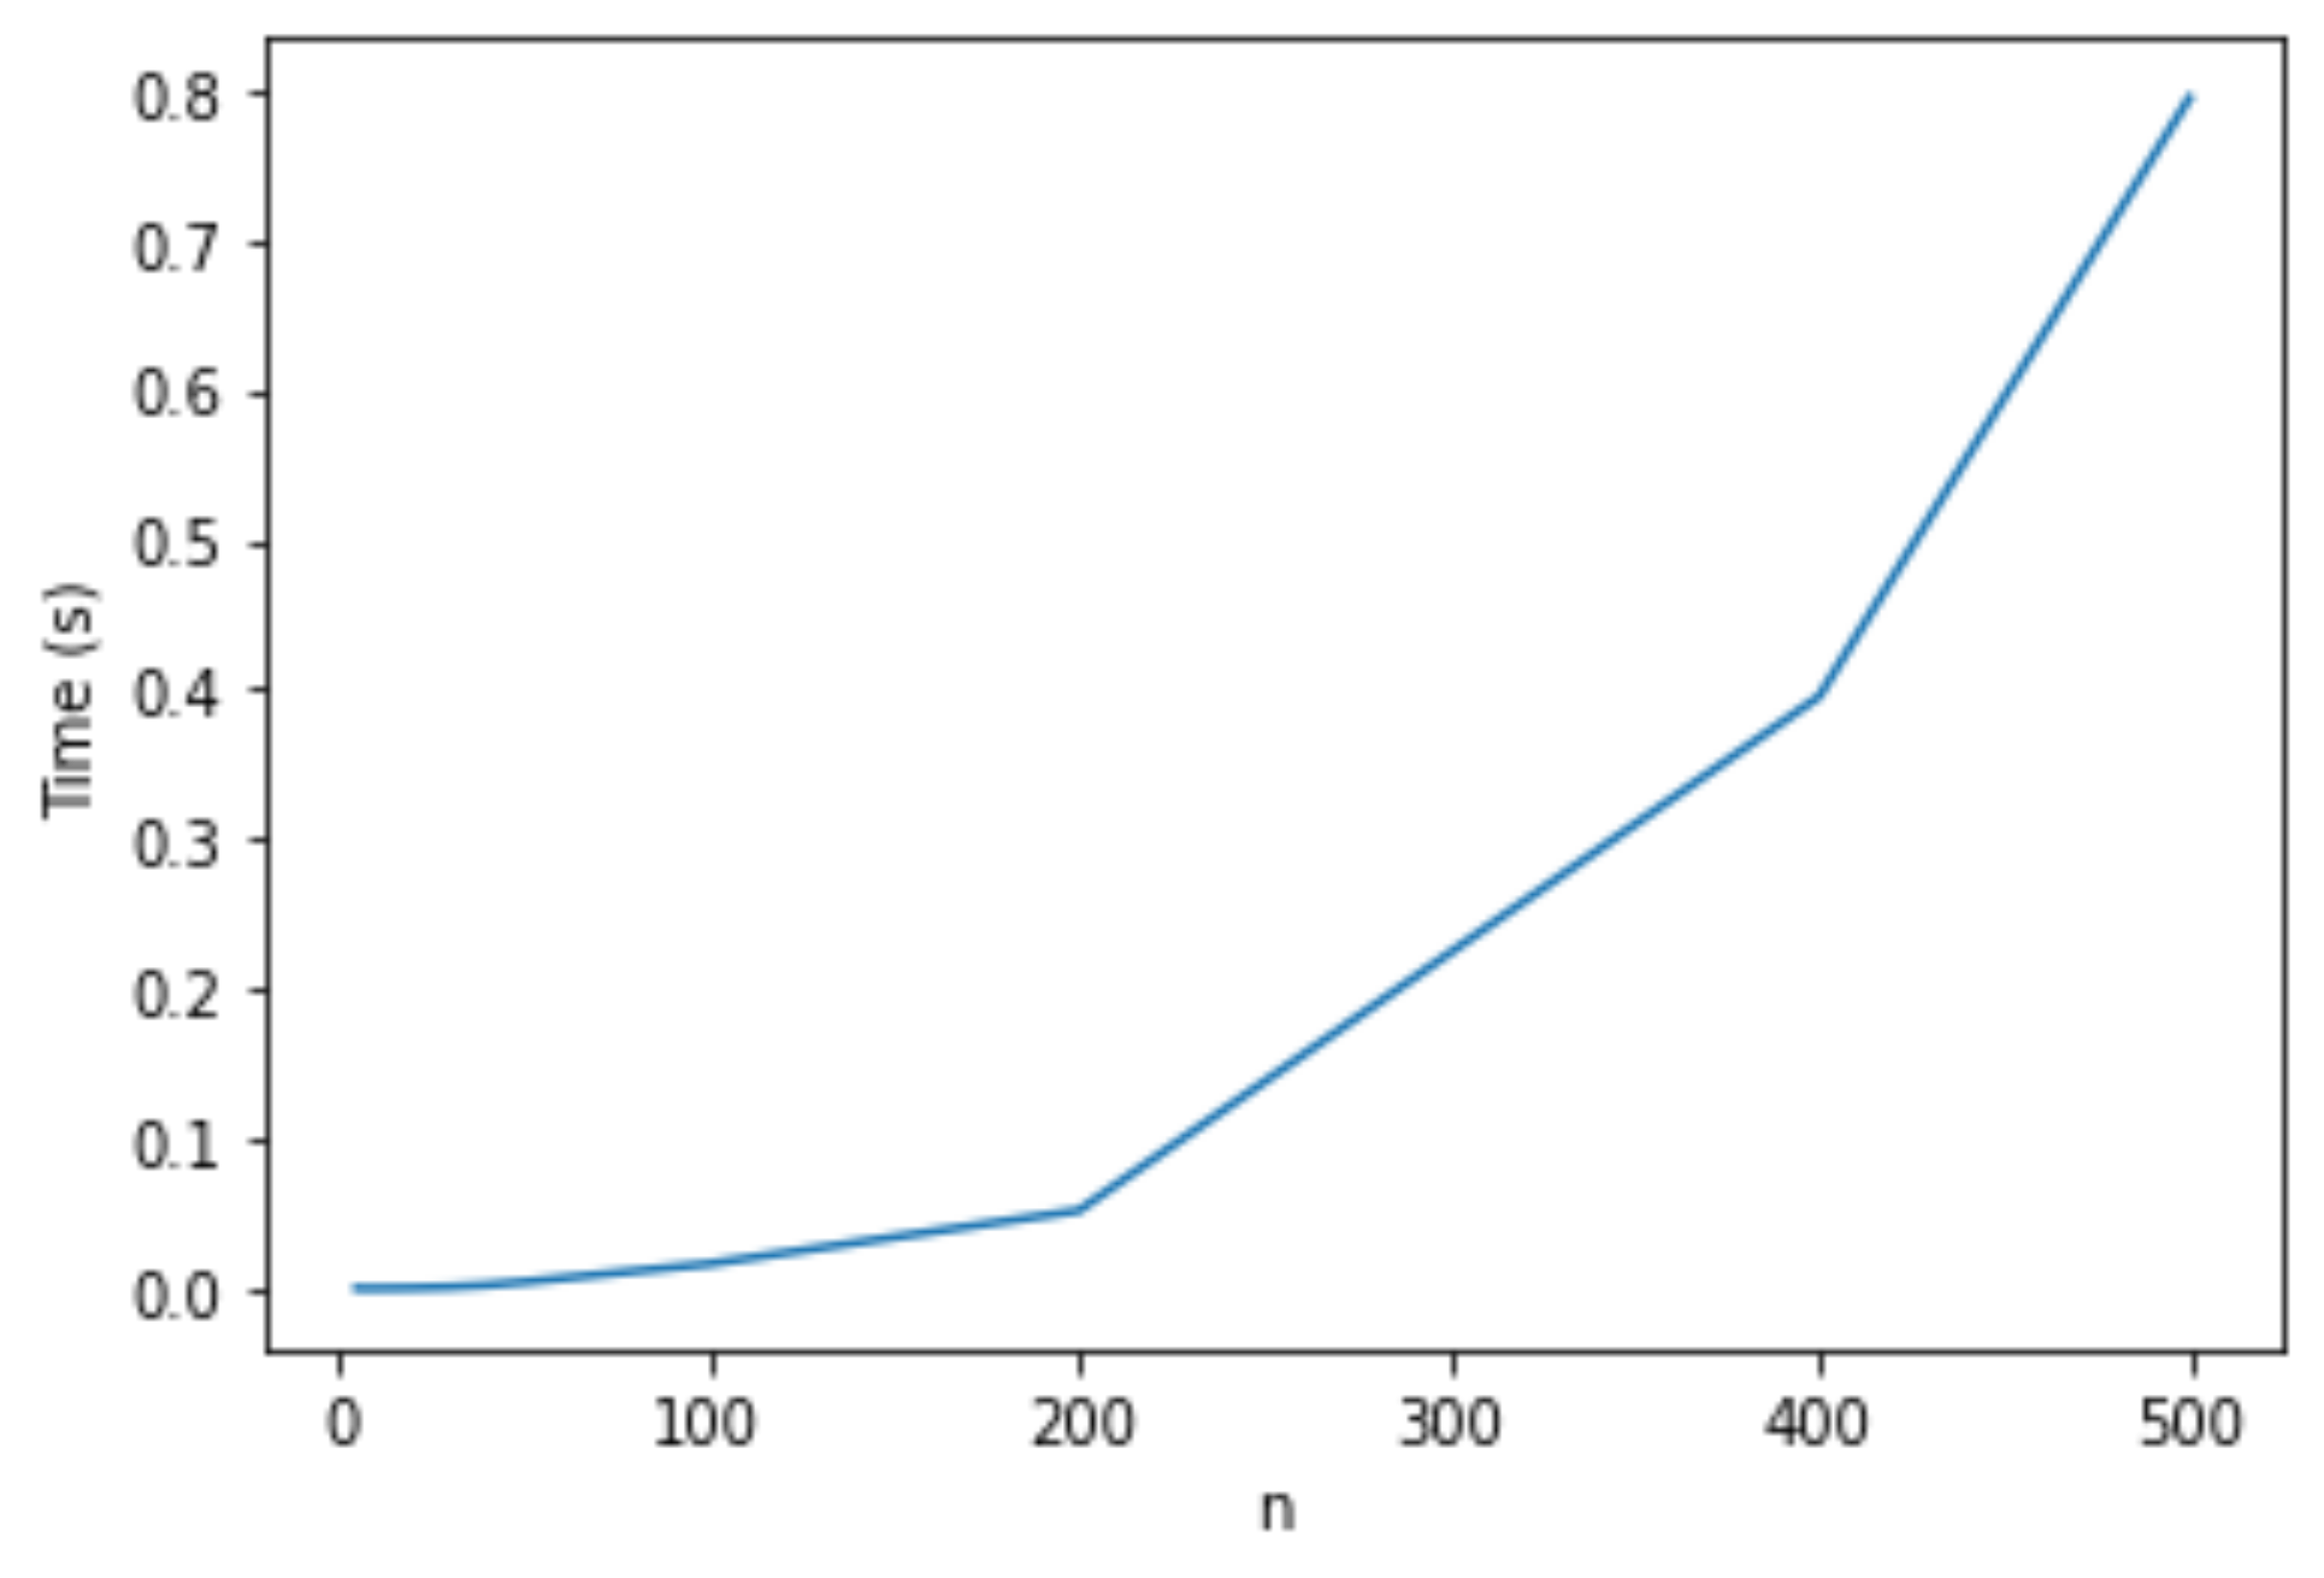
\includegraphics[width=1\linewidth]{figures/tempoTri.png}
					\end{center}
				\end{figure}
			\end{minipage}
			\hspace{0.1cm}
			\begin{minipage}{0.45 \linewidth}
				
				\begin{figure}[H]
					\begin{center}
						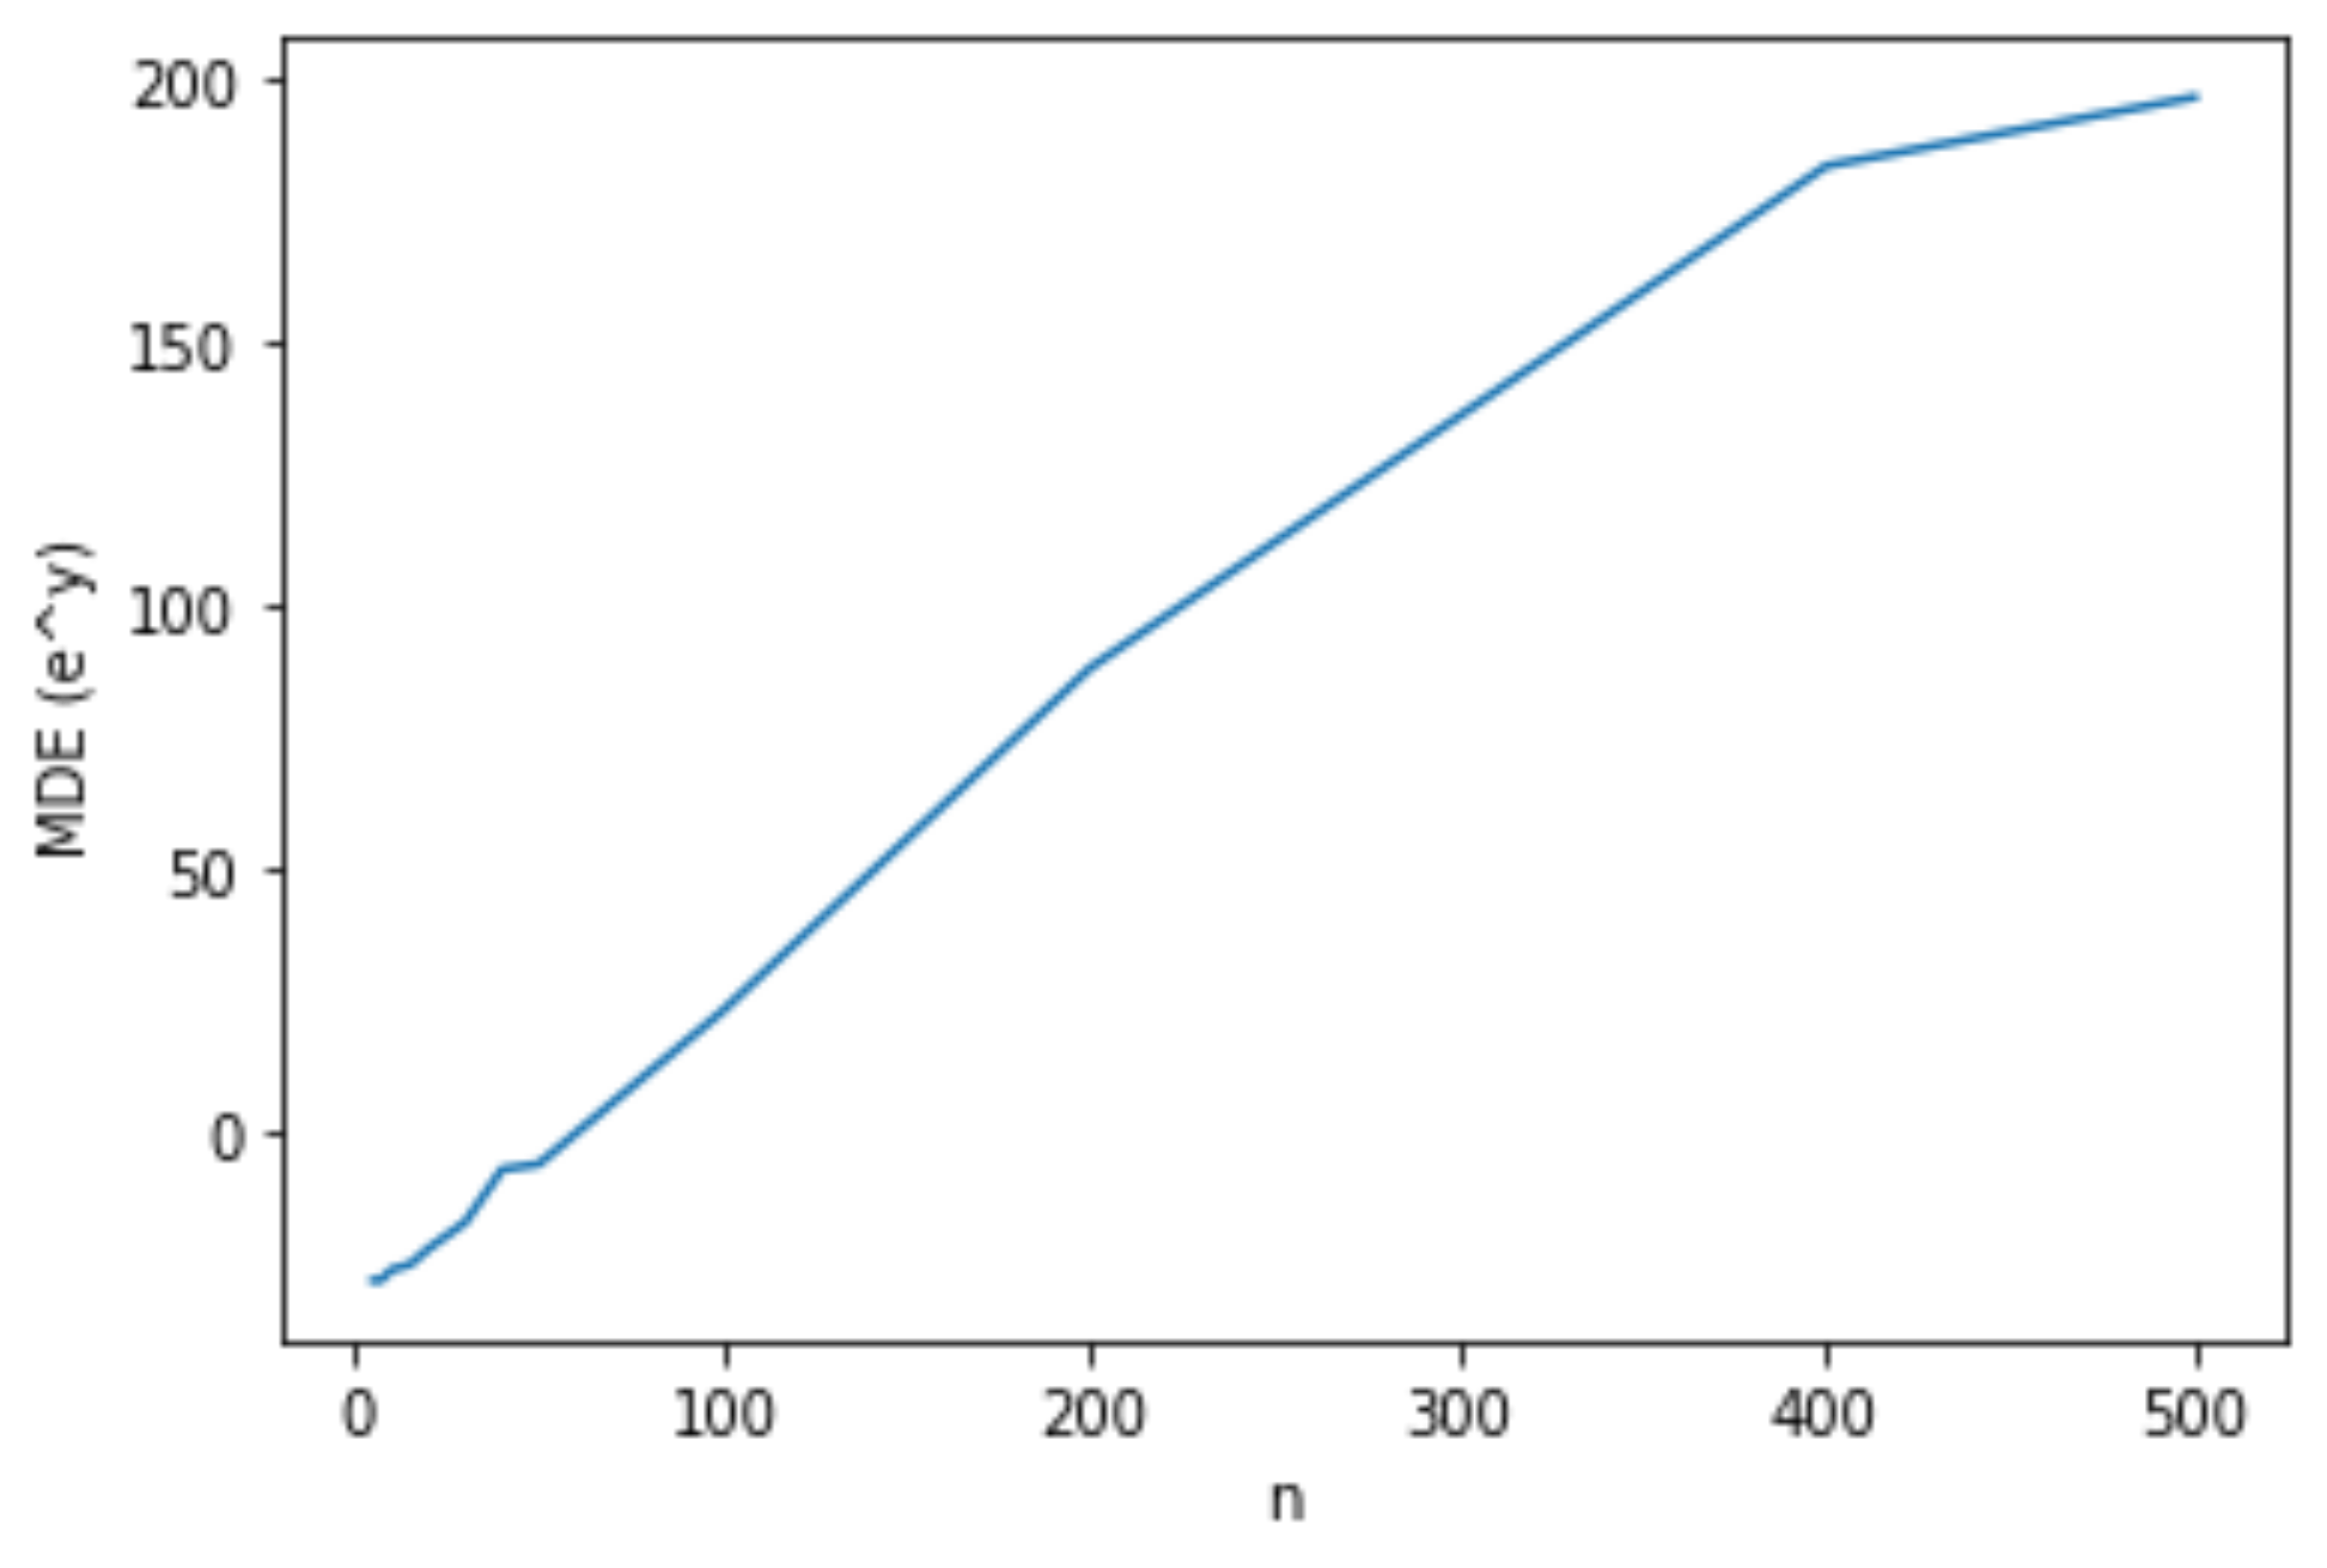
\includegraphics[width=1\linewidth]{figures/mdeTri.png}
					\end{center}
				\end{figure}
			\end{minipage}
		\end{center}
		\caption{A esquerda, o tempo de processo e, a direita, a ordem de grandeza associada ao MDE das soluções.}
		\label{fig:tri}
	\end{figure}
	
	Perceba o comportamento mostrado na Figura~\ref{fig:tri}. Teve-se que fazer uma linearização no gráfico que representa o MDE da solução, pois este cresceu exponencialmente e foi para a ordem de $10^{200}$ em 500 vértices. Esse comportamento se deu por conta dos erros acumulados entre as iterações.
	\\
	
	Uma proposta pensada para contornar essa situação infeliz foi alterar o valor de $\mathcal{P}$, deixando o menor, obrigando o algorítimo a calcular realizações utilizando vértices iniciais. Porém, isso implicaria em um grafo não completo, o que não condiz definição do Algorítimo~\ref{alg:realizacaoIterativa}.
	
	Outra solução proposta fora de utilizar sempre os primeiros vértices no lugar dos antecessores mais próximos. Isso significaria utilizar sempre os vértices âncoras para realizar os demais, semelhante com o que é feito no sistema GPS. Com isso, tivemos os resultados satisfatórios apresentados pela Figura~\ref{fig:triPri}. Perceba que mesmo com 500 vértices ainda obteve-se resultados com $MDE$ na ordem de $10^{-20}$.
	
	\begin{figure}[H]
		\begin{center}
			\begin{minipage}{0.45 \linewidth}
				\begin{figure}[H]
					\begin{center}
						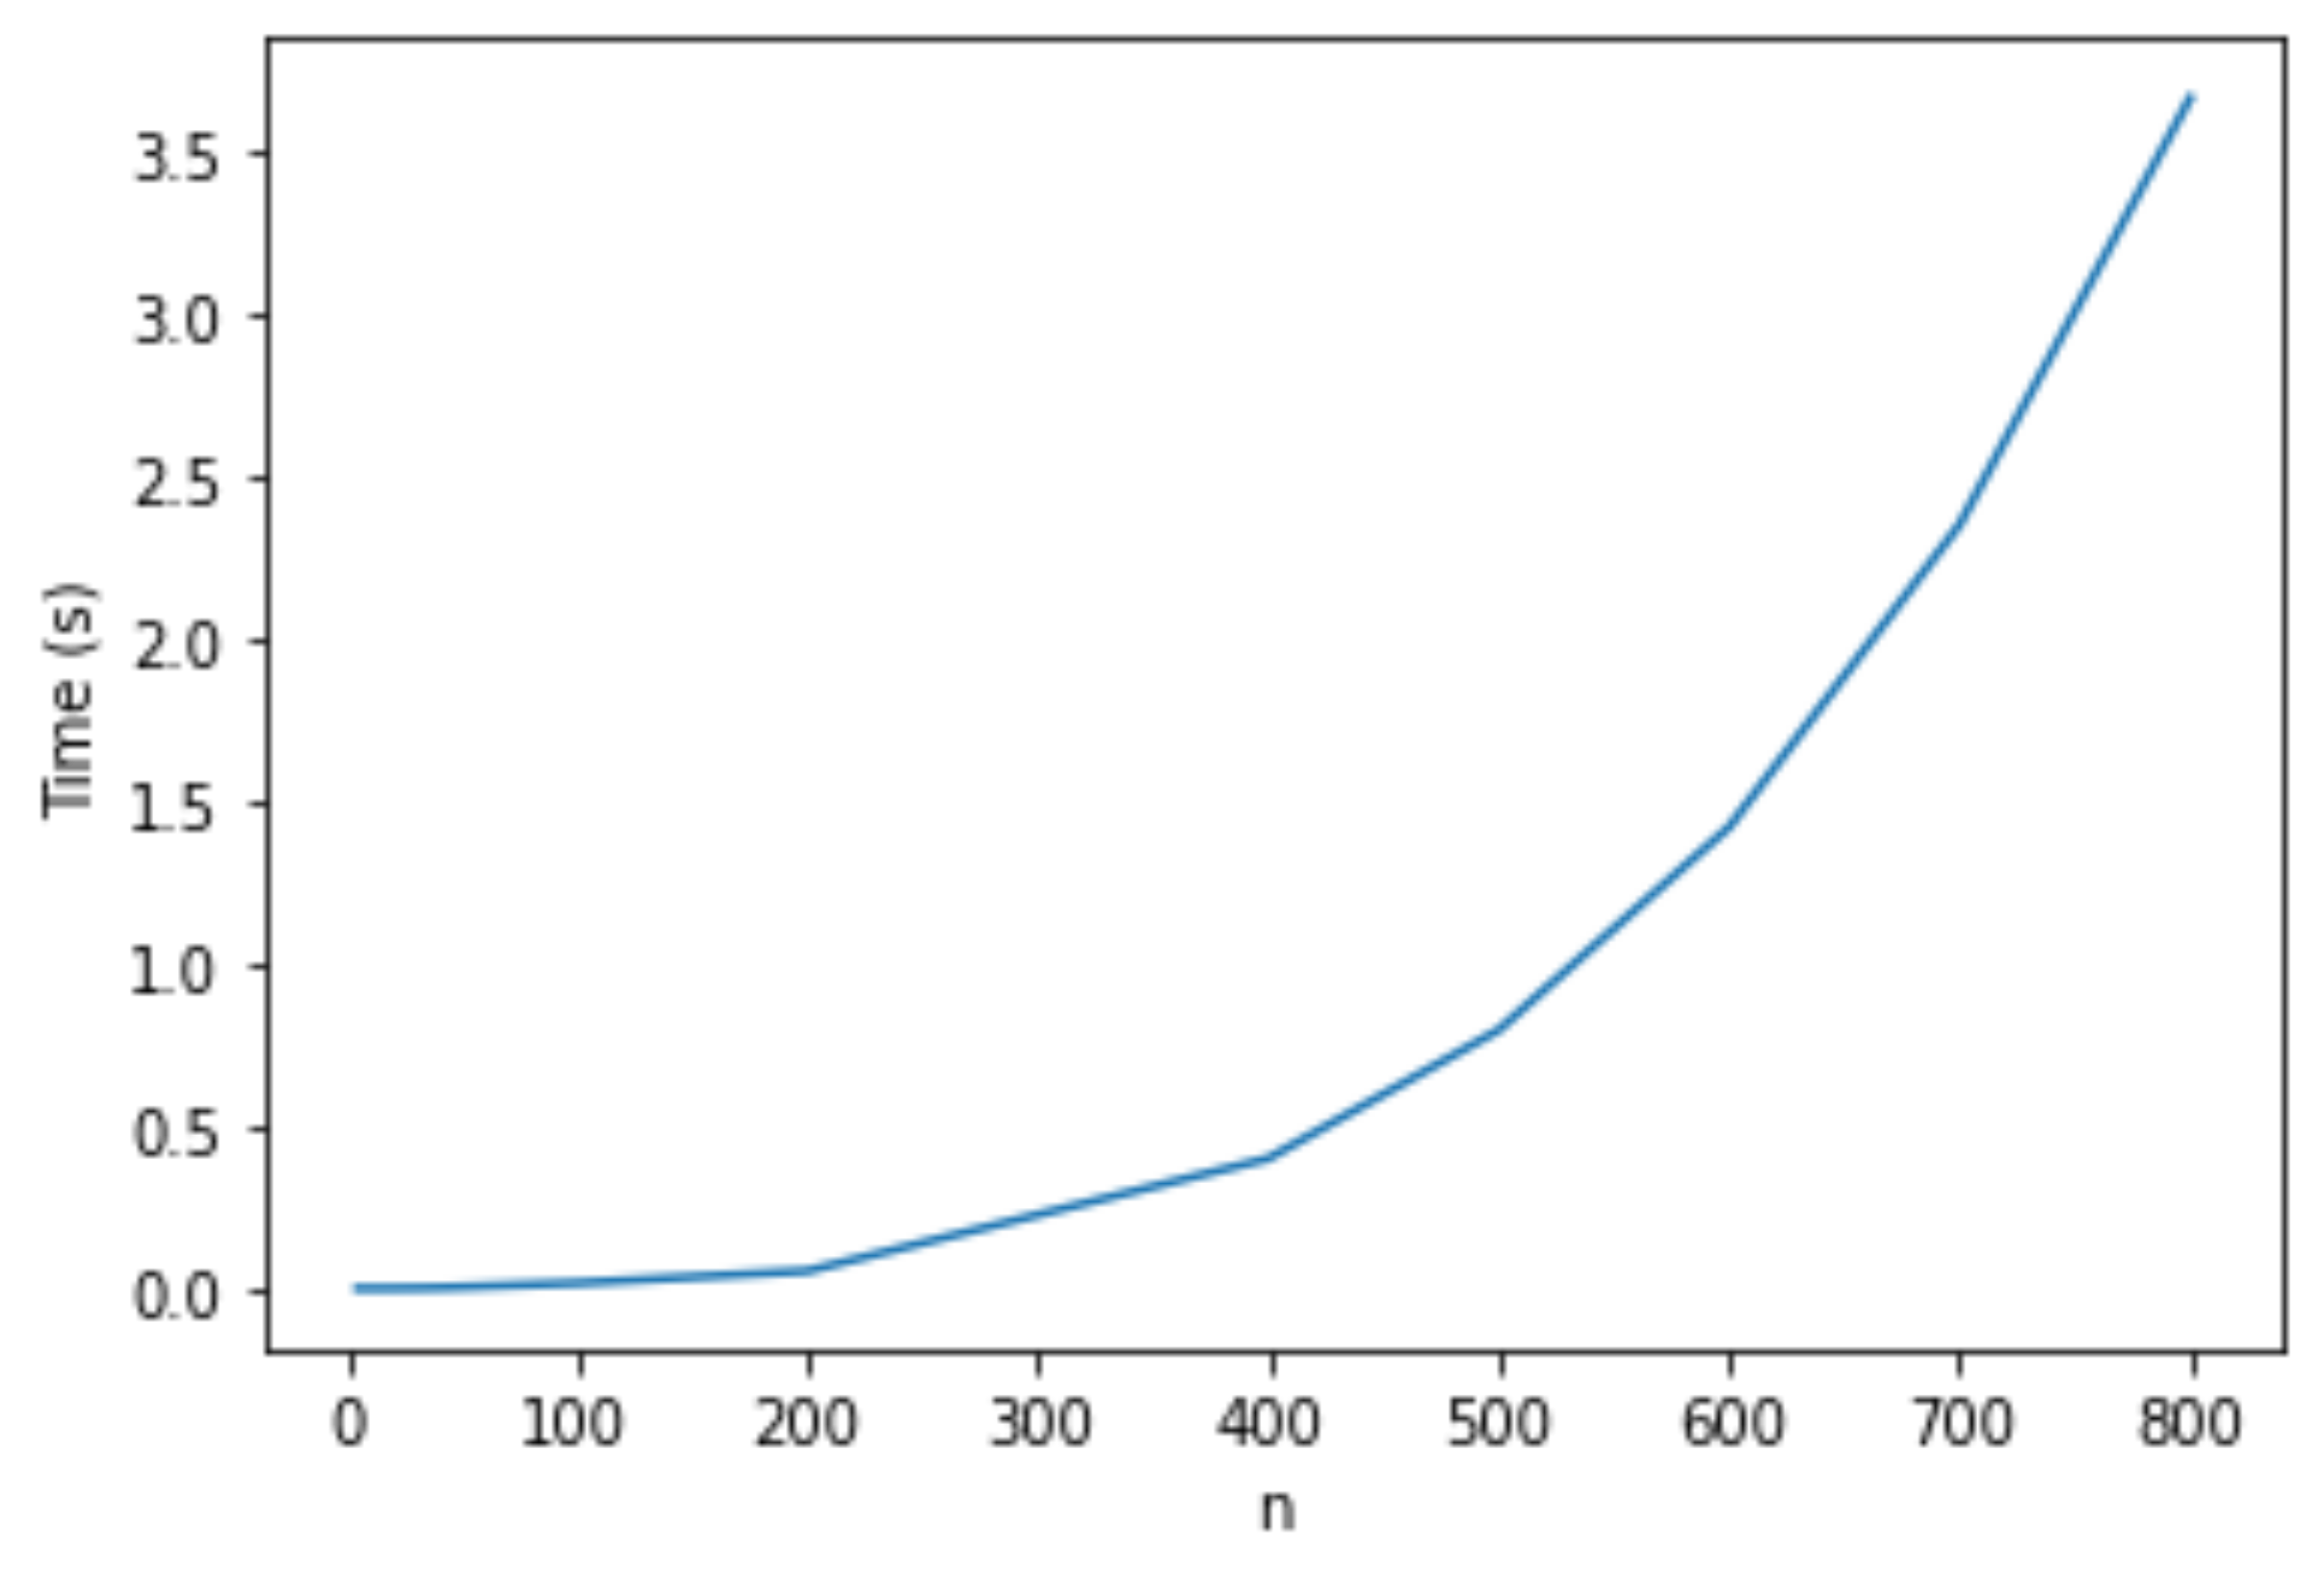
\includegraphics[width=1\linewidth]{figures/tempoTriPri.png}
					\end{center}
				\end{figure}
			\end{minipage}
			\hspace{0.1cm}
			\begin{minipage}{0.45 \linewidth}
				
				\begin{figure}[H]
					\begin{center}
						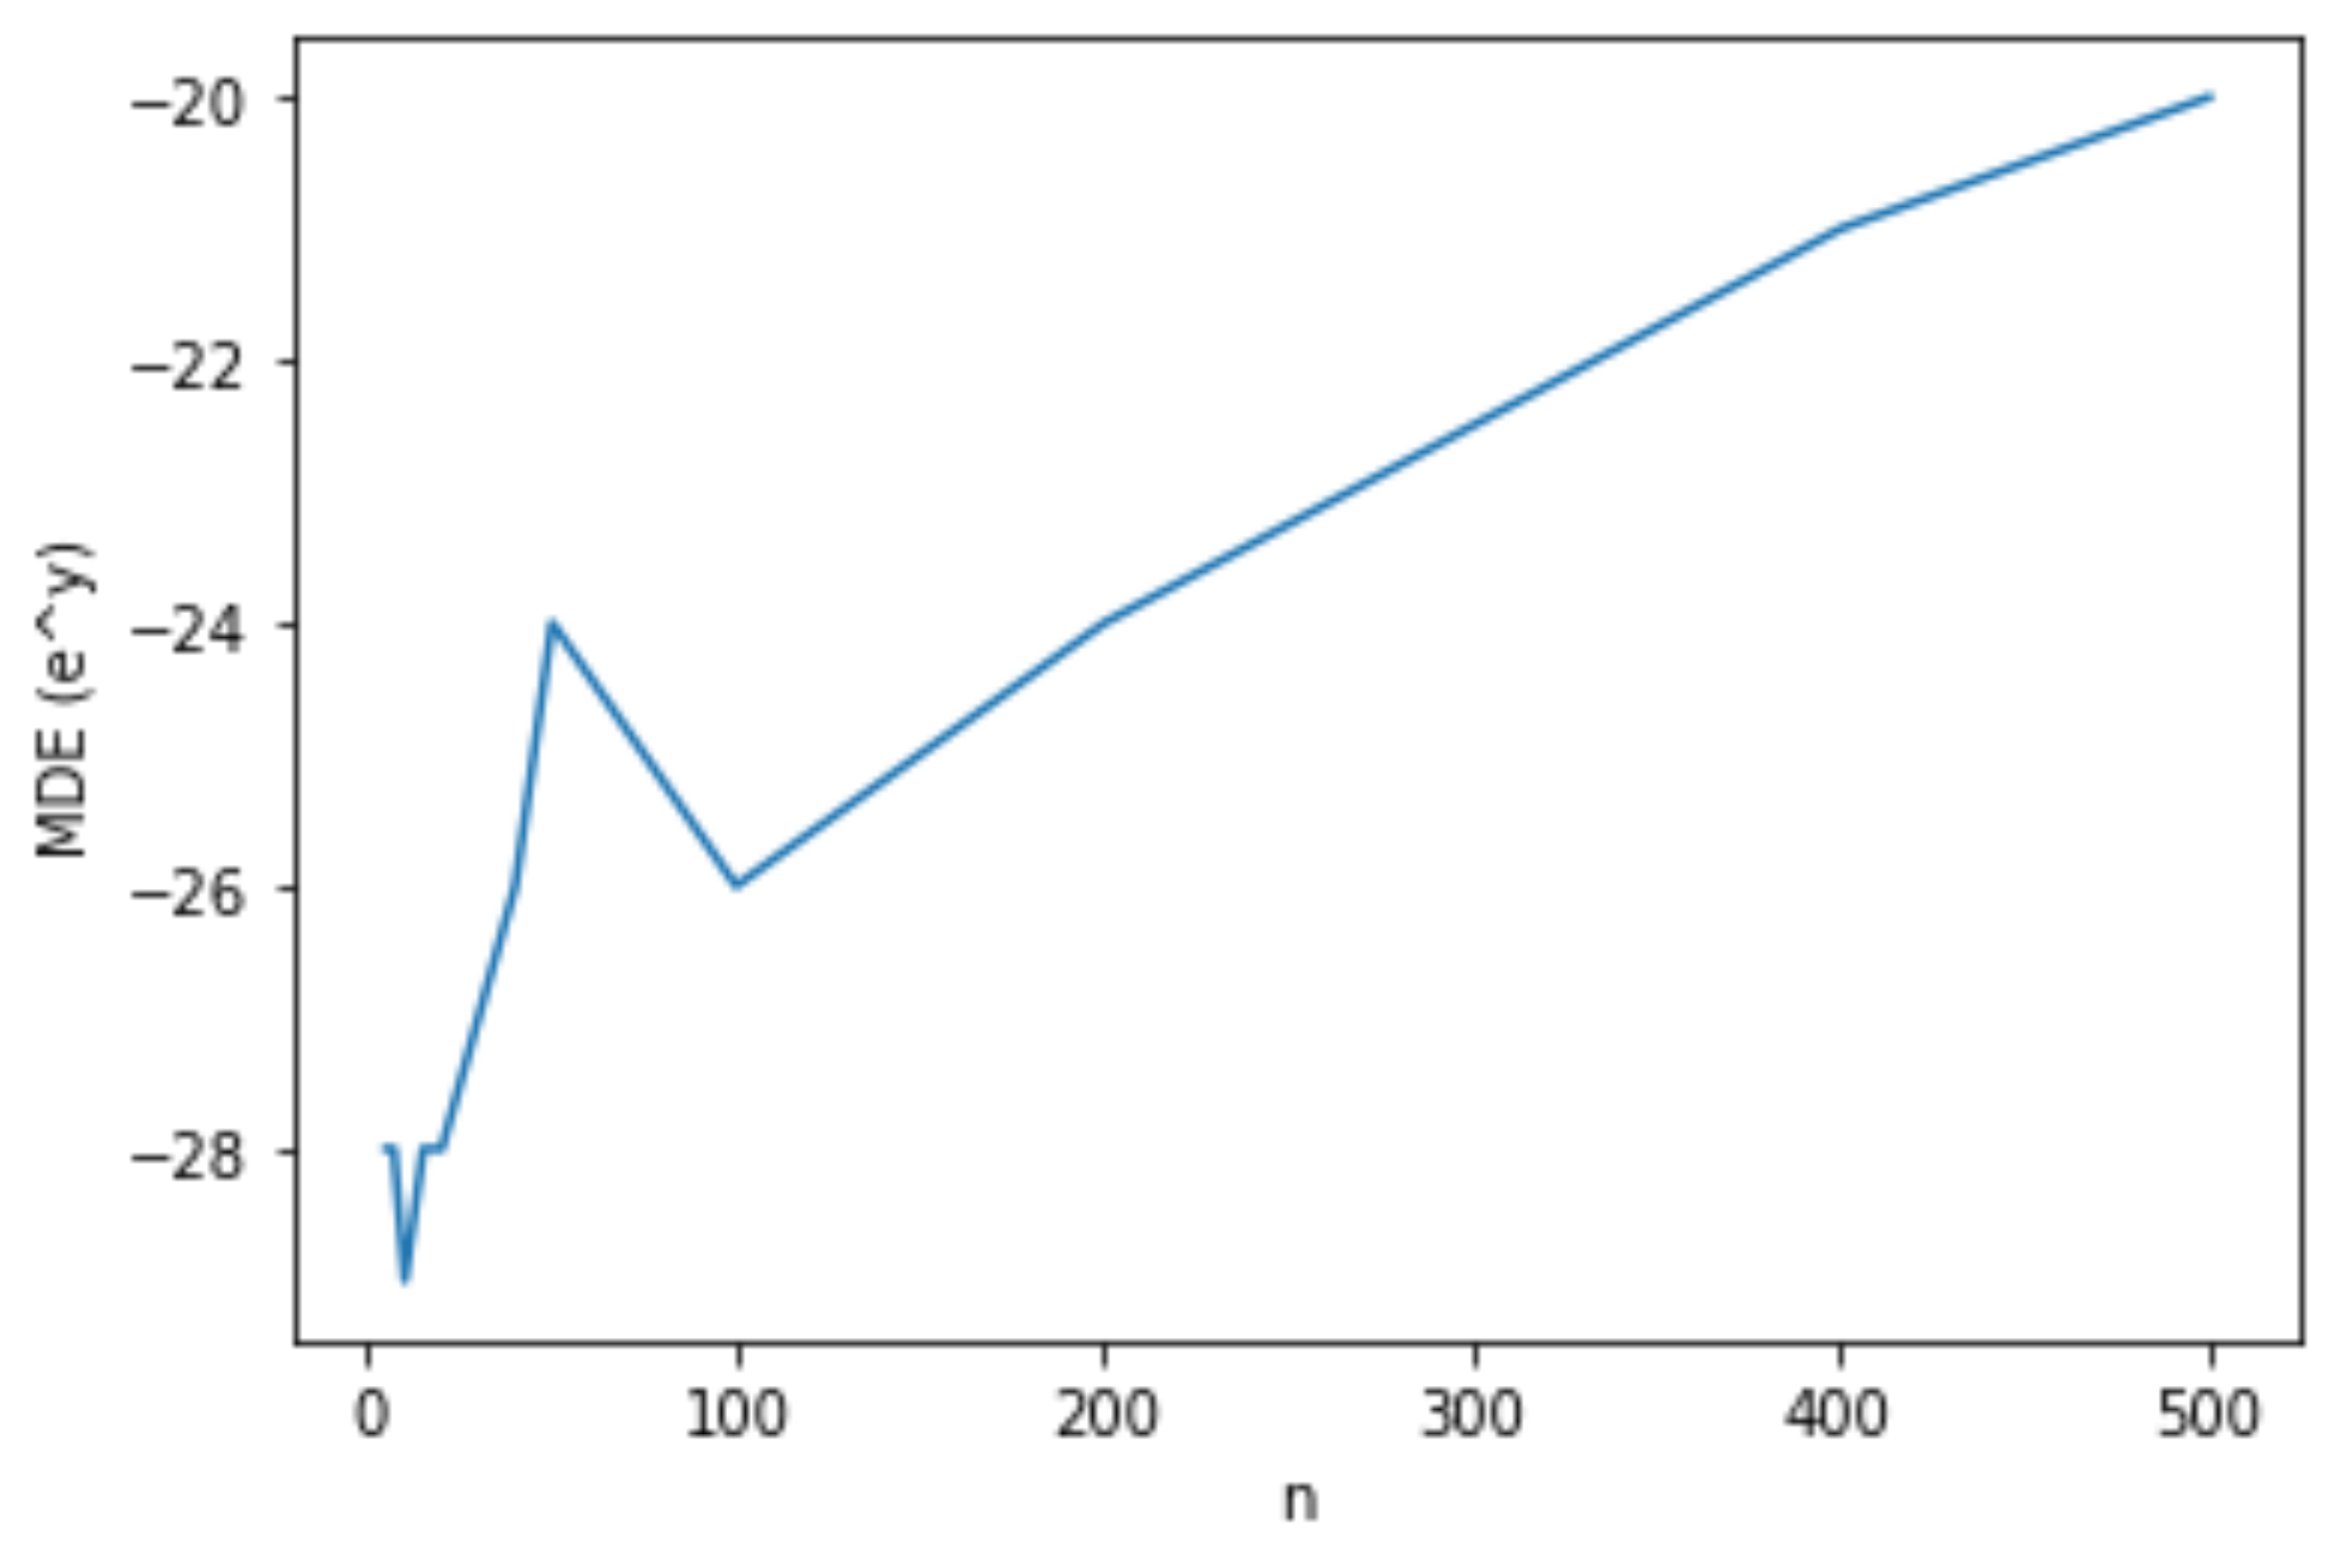
\includegraphics[width=1\linewidth]{figures/mdeTriPro.png}
					\end{center}
					\label{fig:mdeTri}
				\end{figure}
			\end{minipage}
		\end{center}
		\caption{A esquerda, o tempo de processo e, a direita, a ordem de grandeza associada ao MDE das soluções.}
		\label{fig:triPri}
	\end{figure}
	
	Também simulou-se o Algorítimo~\ref{alg:realizacaoTrilateration}, que teve um comportamento muito similar ao Algorítimo~\ref{alg:realizacaoIterativa}, como era de se esperar. Também usou-se instâncias $n$ variando em $\{5, 6, 7,10,15,20,30,40,50,100,200,400,500\}$. Porém, agora, com uma busca inteligente por vértices adjacentes, pode-se variar $\mathcal{P}$ afim de analisar diferentes geometrias para o problema, como apresenta-se a seguir.
	
	\subsubsection*{Instâncias com 70\% de arestas}
	
	\begin{figure}[H]
		\begin{center}
			\begin{minipage}{0.45 \linewidth}
				\begin{figure}[H]
					\begin{center}
						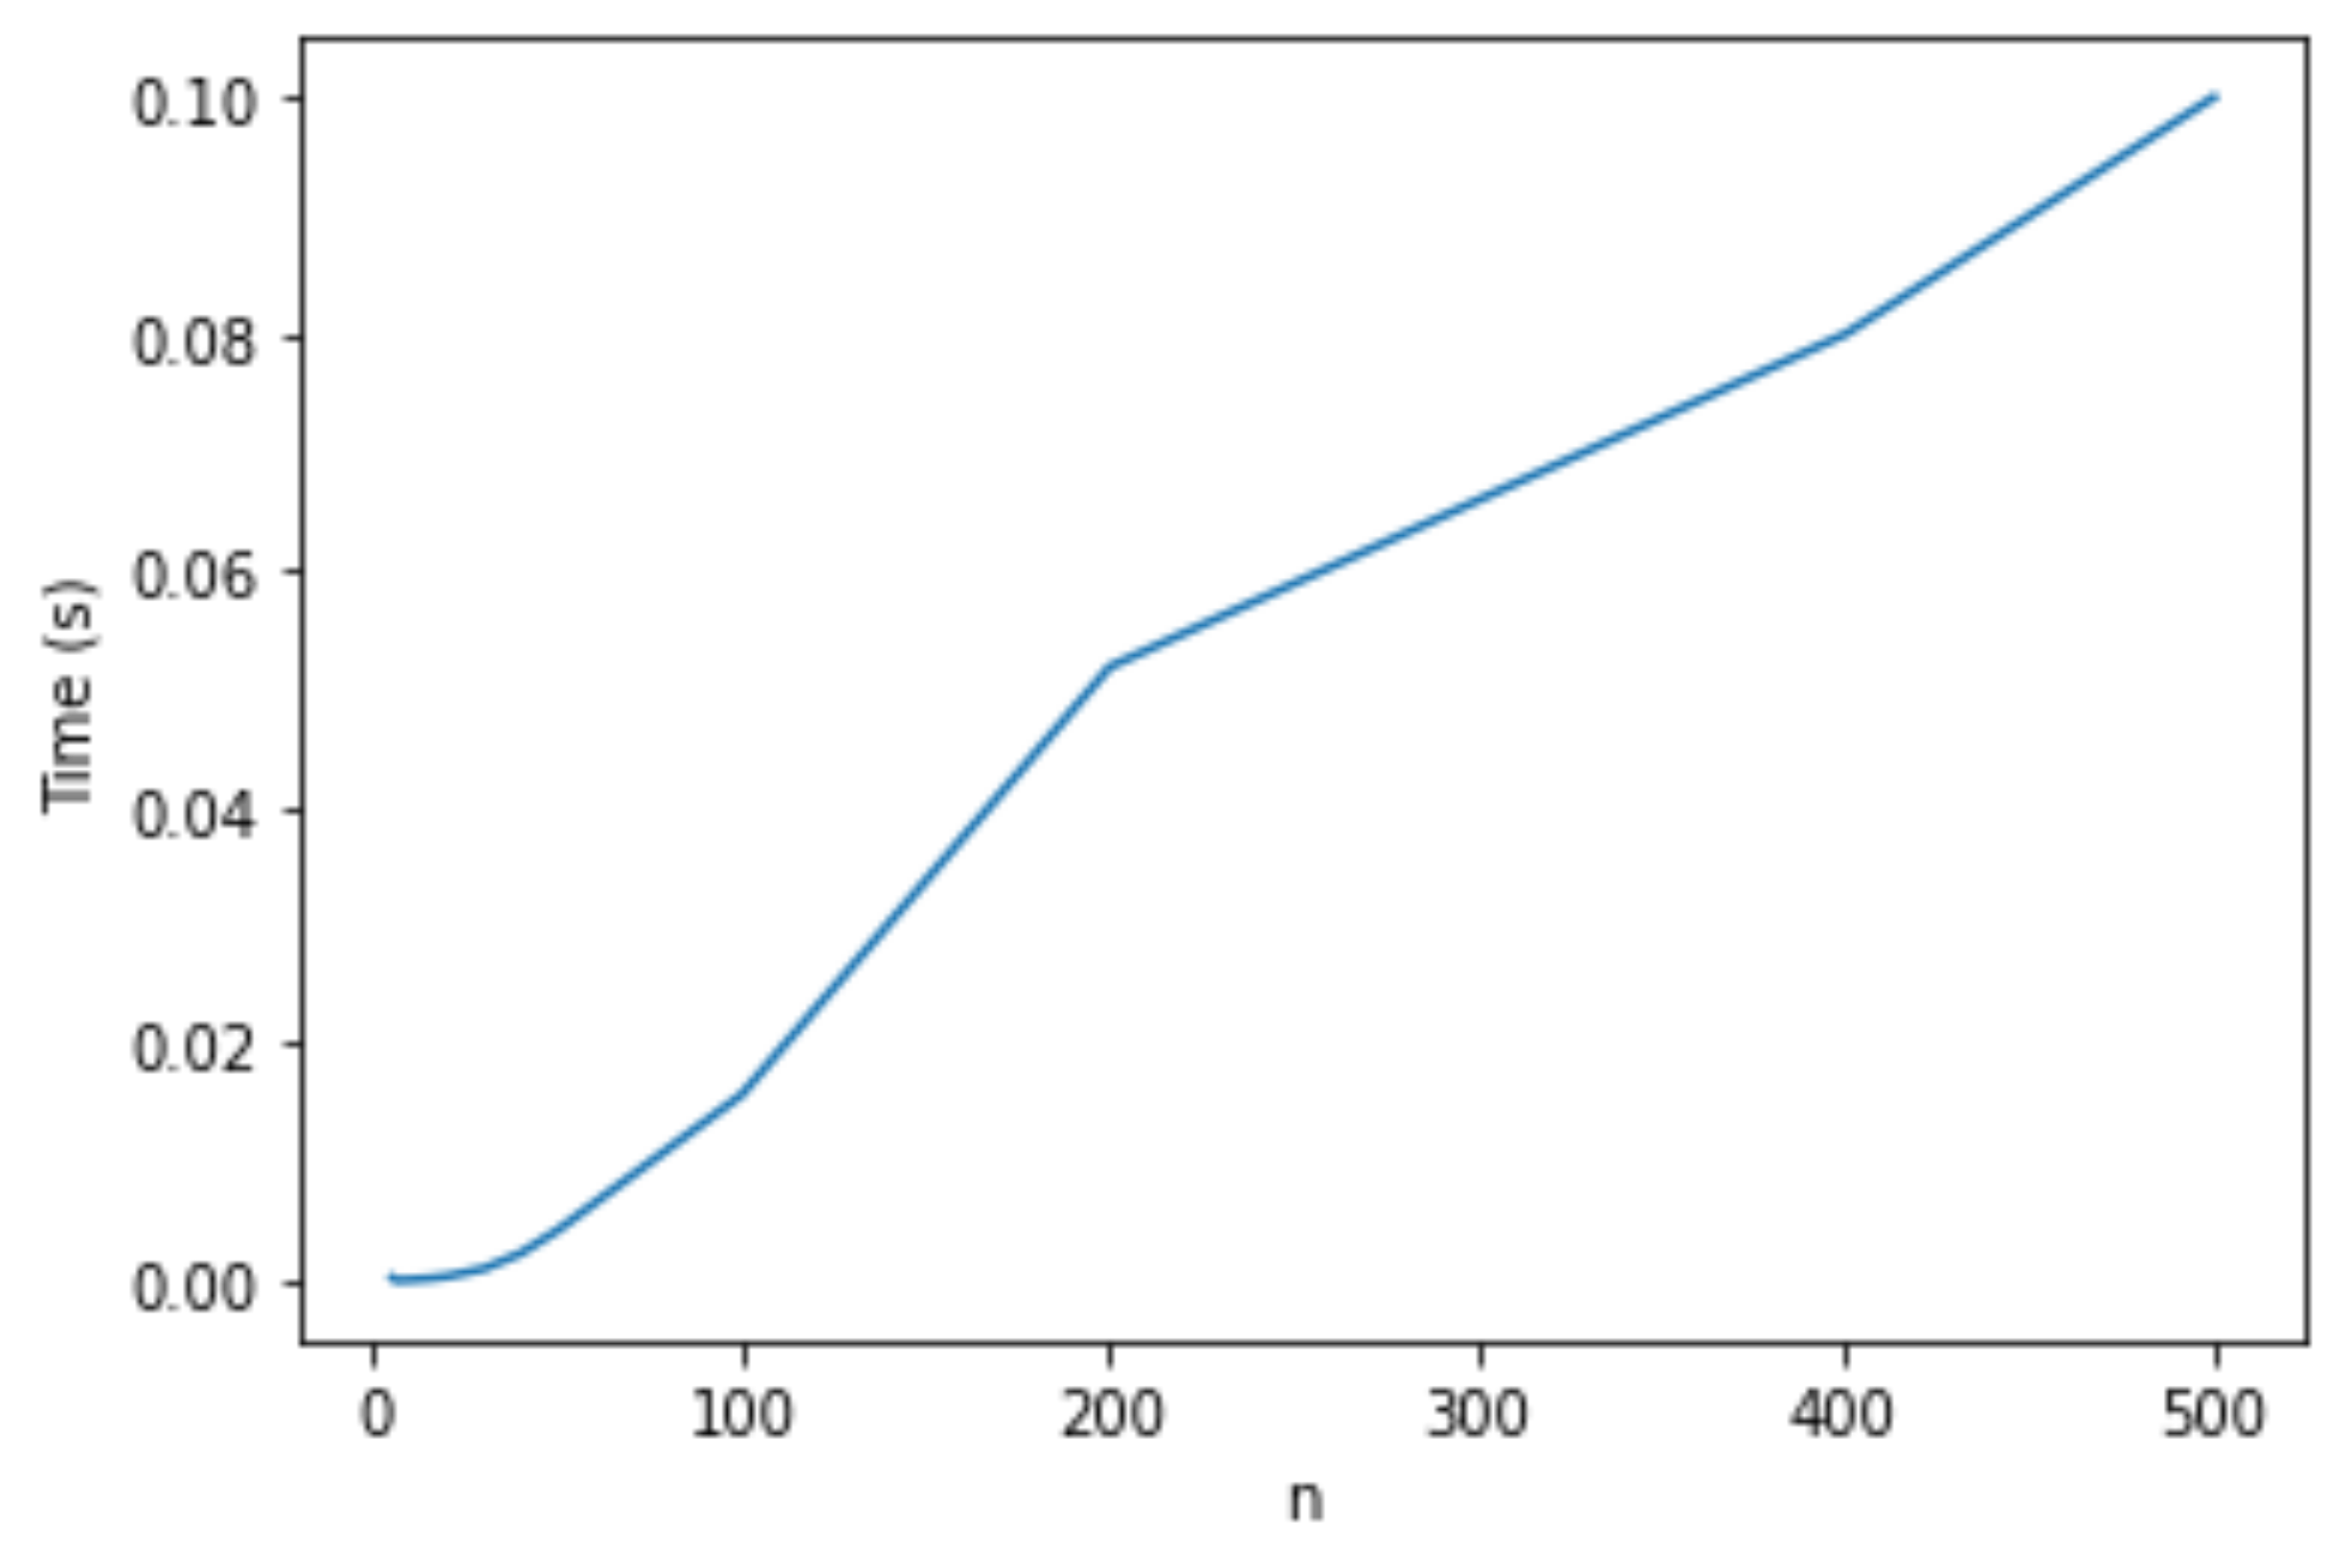
\includegraphics[width=1\linewidth]{figures/timeTriPro1.png}
					\end{center}
				\end{figure}
			\end{minipage}
			\hspace{0.1cm}
			\begin{minipage}{0.45 \linewidth}
				
				\begin{figure}[H]
					\begin{center}
						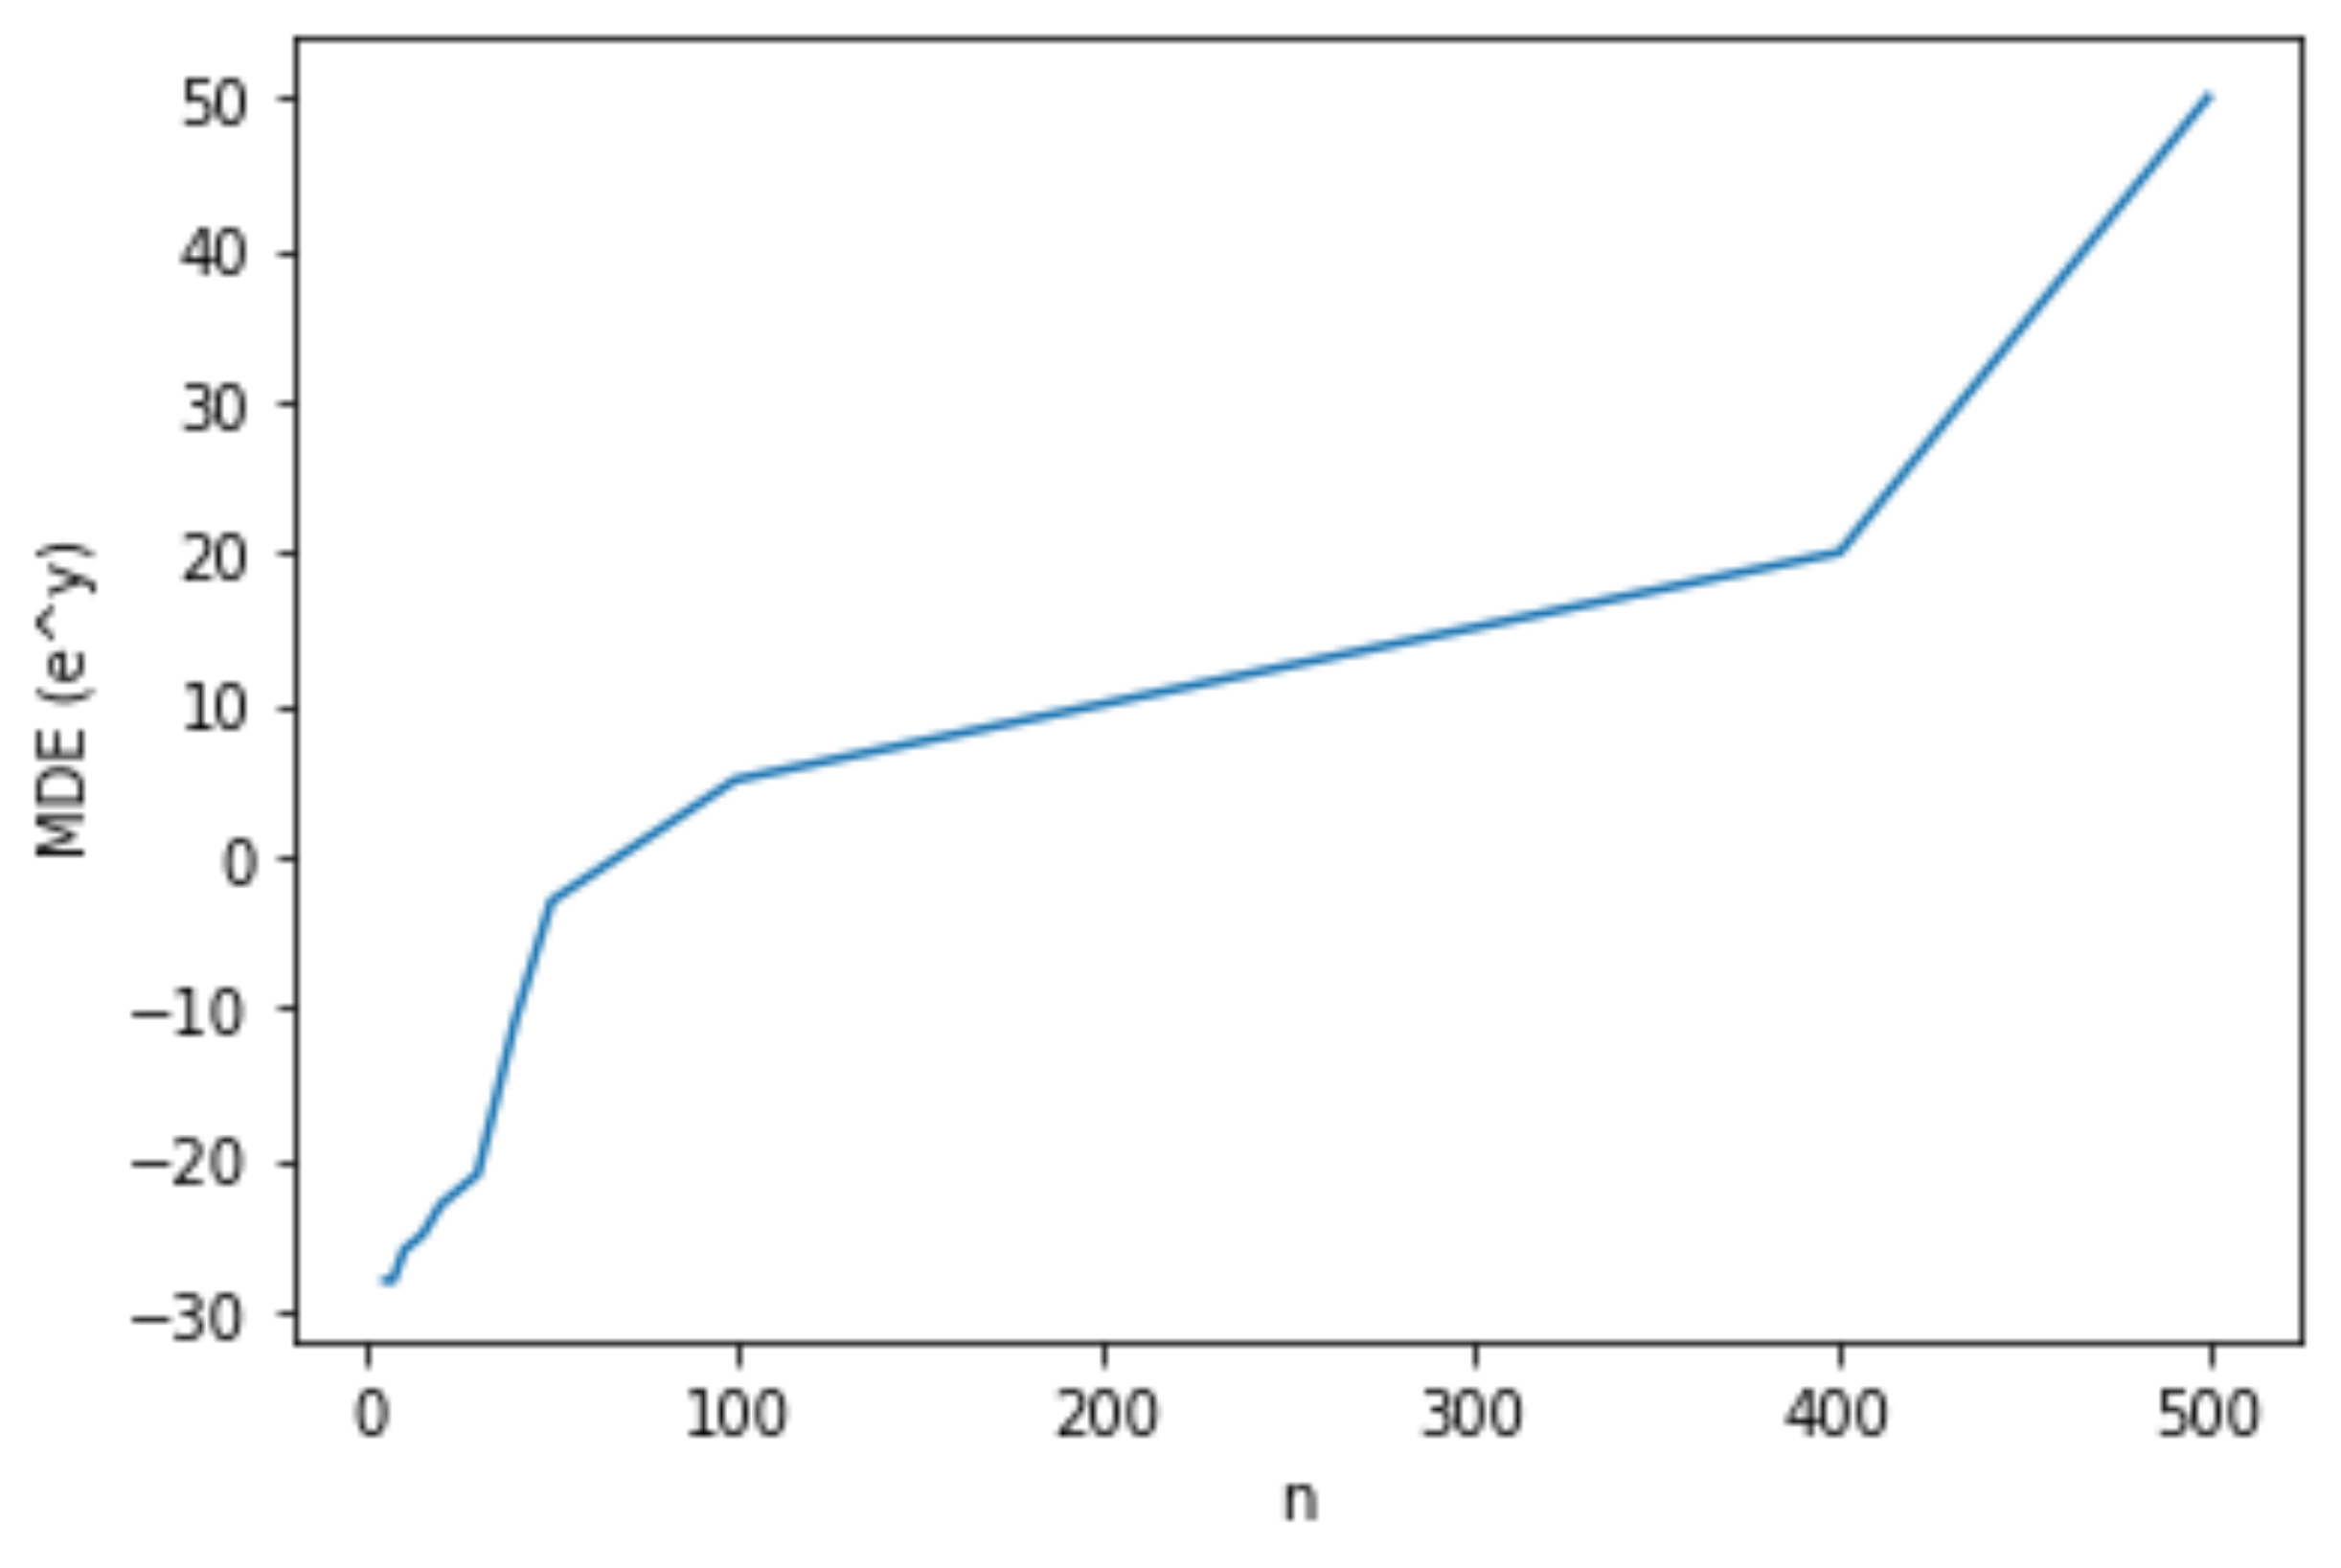
\includegraphics[width=1\linewidth]{figures/mdeTriPro1.png}
					\end{center}
					\label{fig:mdeTri}
				\end{figure}
			\end{minipage}
		\end{center}
		\caption{A esquerda, o tempo de processo e, a direita, a ordem de grandeza associada ao MDE das soluções. Utilizou-se $\mathcal{P} = 0.7$.}
		\label{fig:triPri4}
	\end{figure}
	
	\subsubsection*{Instâncias com 5\% de arestas}
	
	\begin{figure}[H]
		\begin{center}
			\begin{minipage}{0.45 \linewidth}
				\begin{figure}[H]
					\begin{center}
						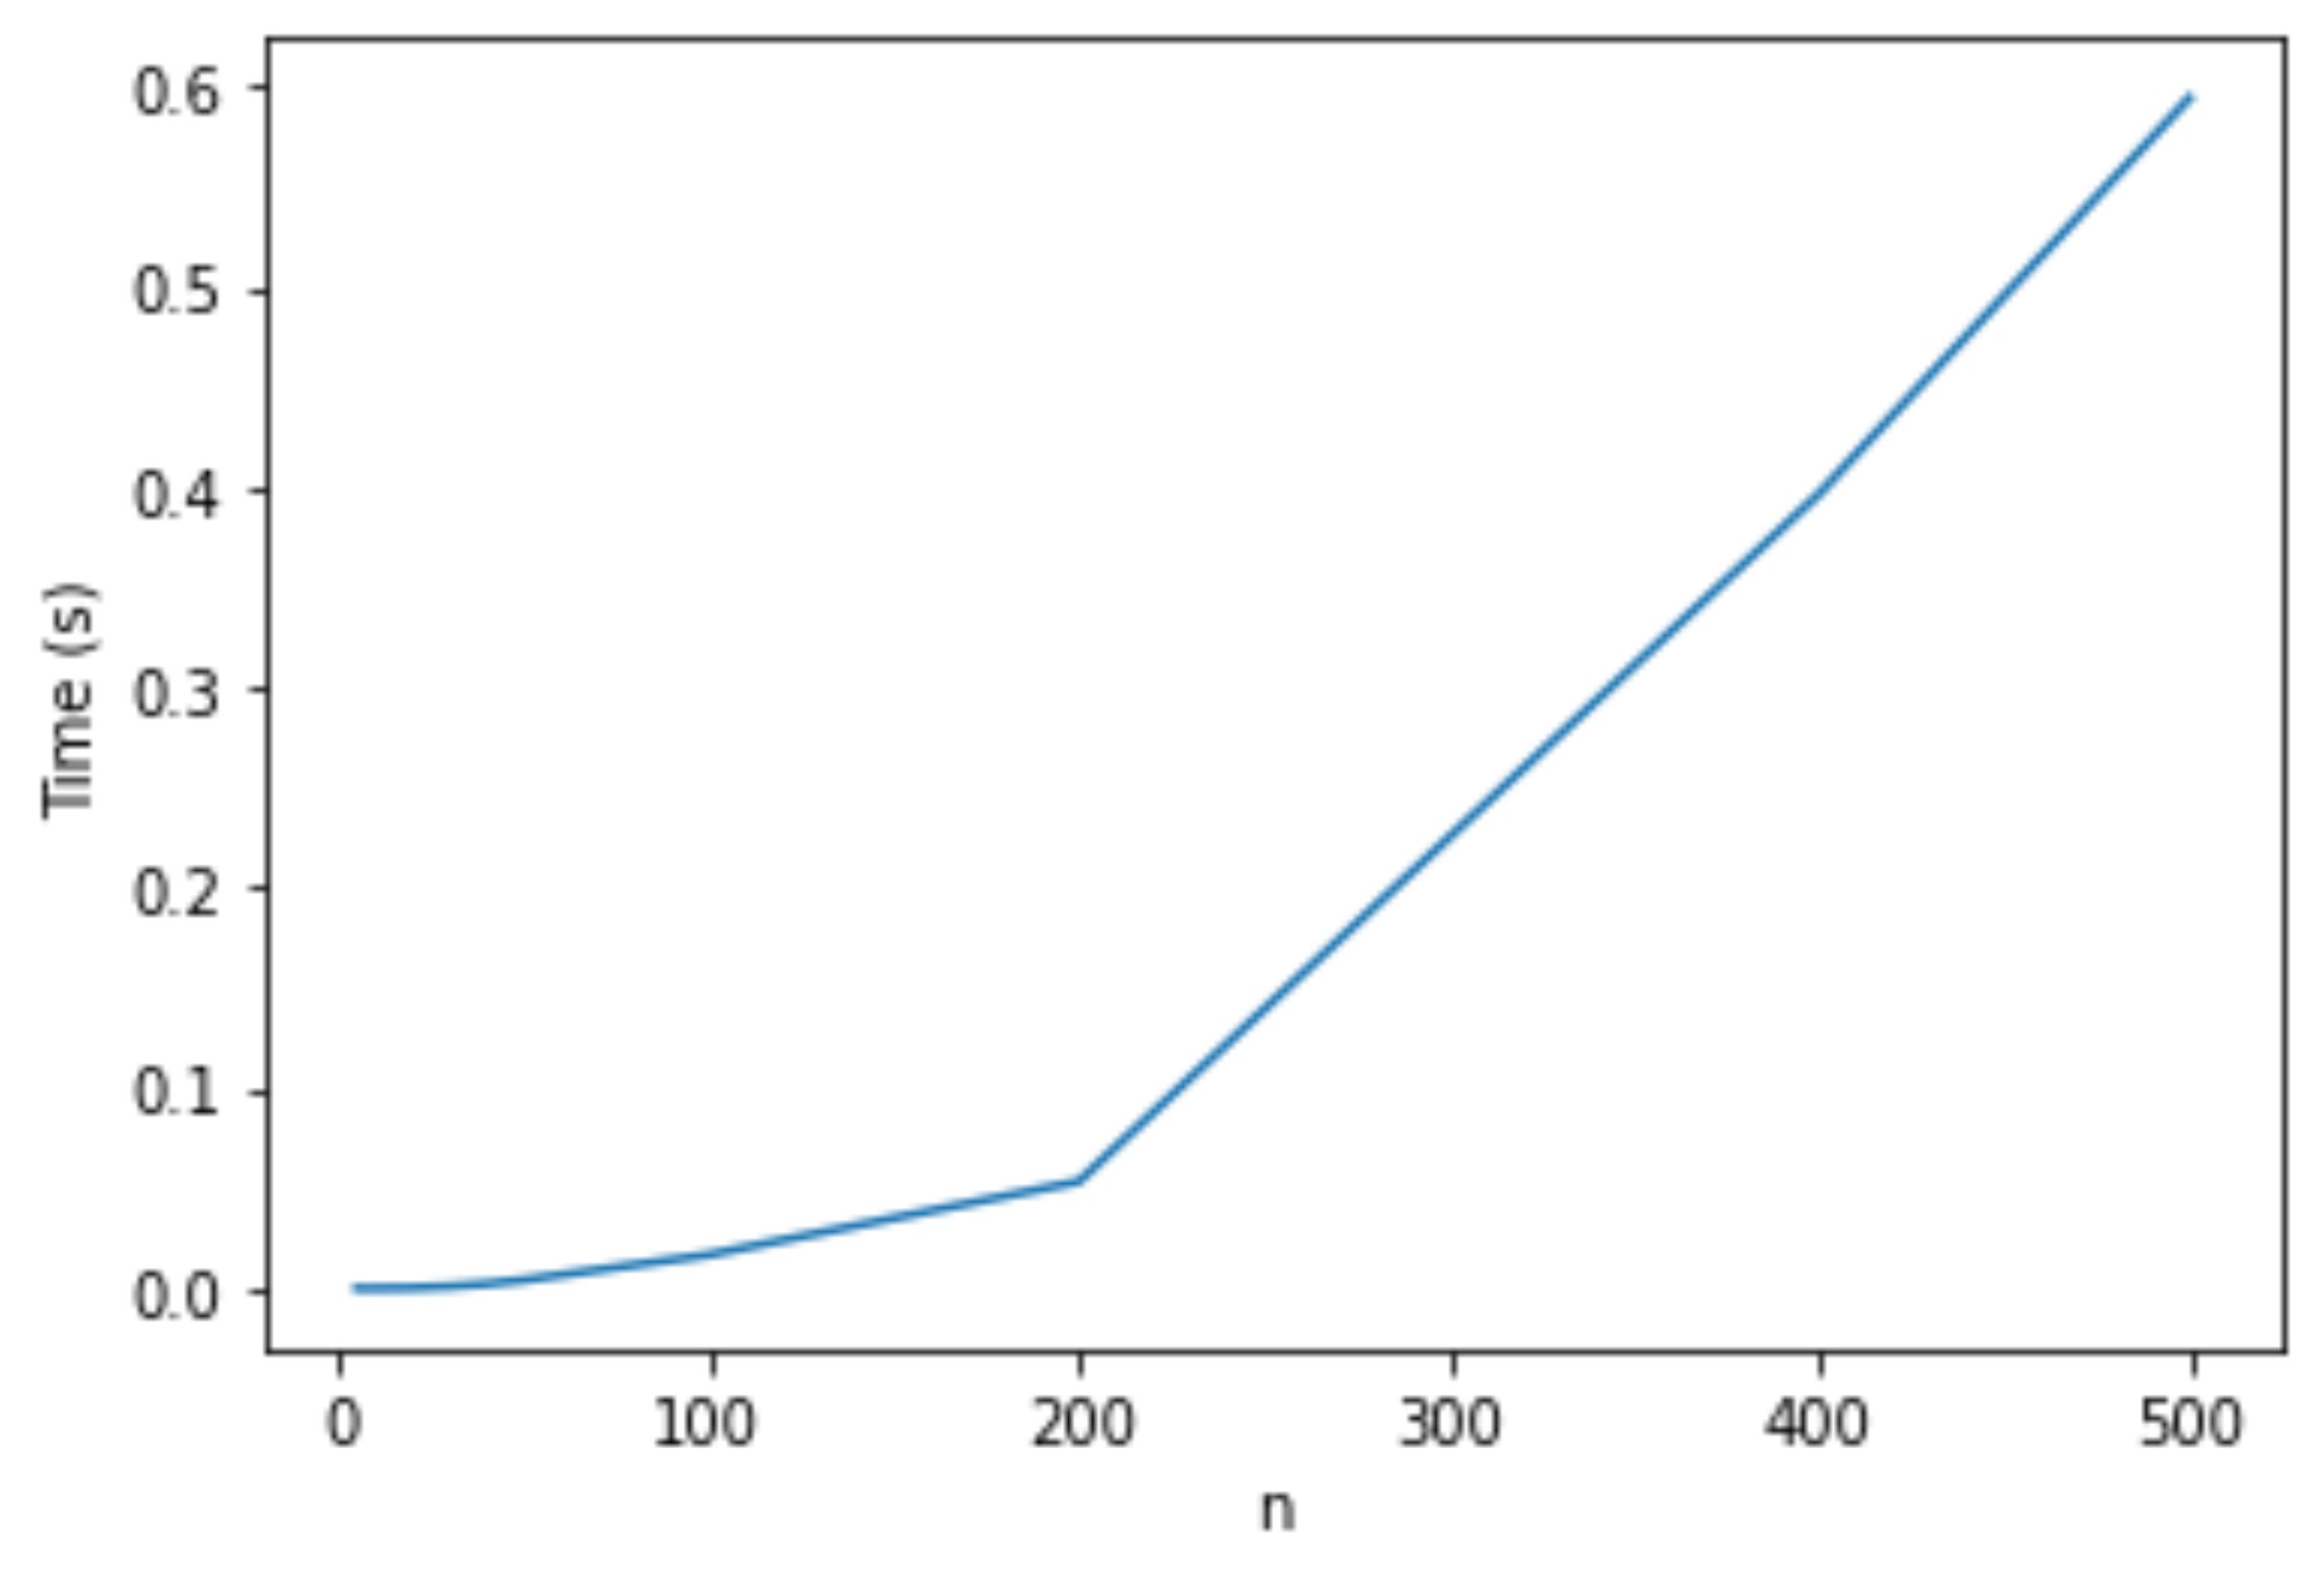
\includegraphics[width=1\linewidth]{figures/timePro2.png}
					\end{center}
				\end{figure}
			\end{minipage}
			\hspace{0.1cm}
			\begin{minipage}{0.45 \linewidth}
				
				\begin{figure}[H]
					\begin{center}
						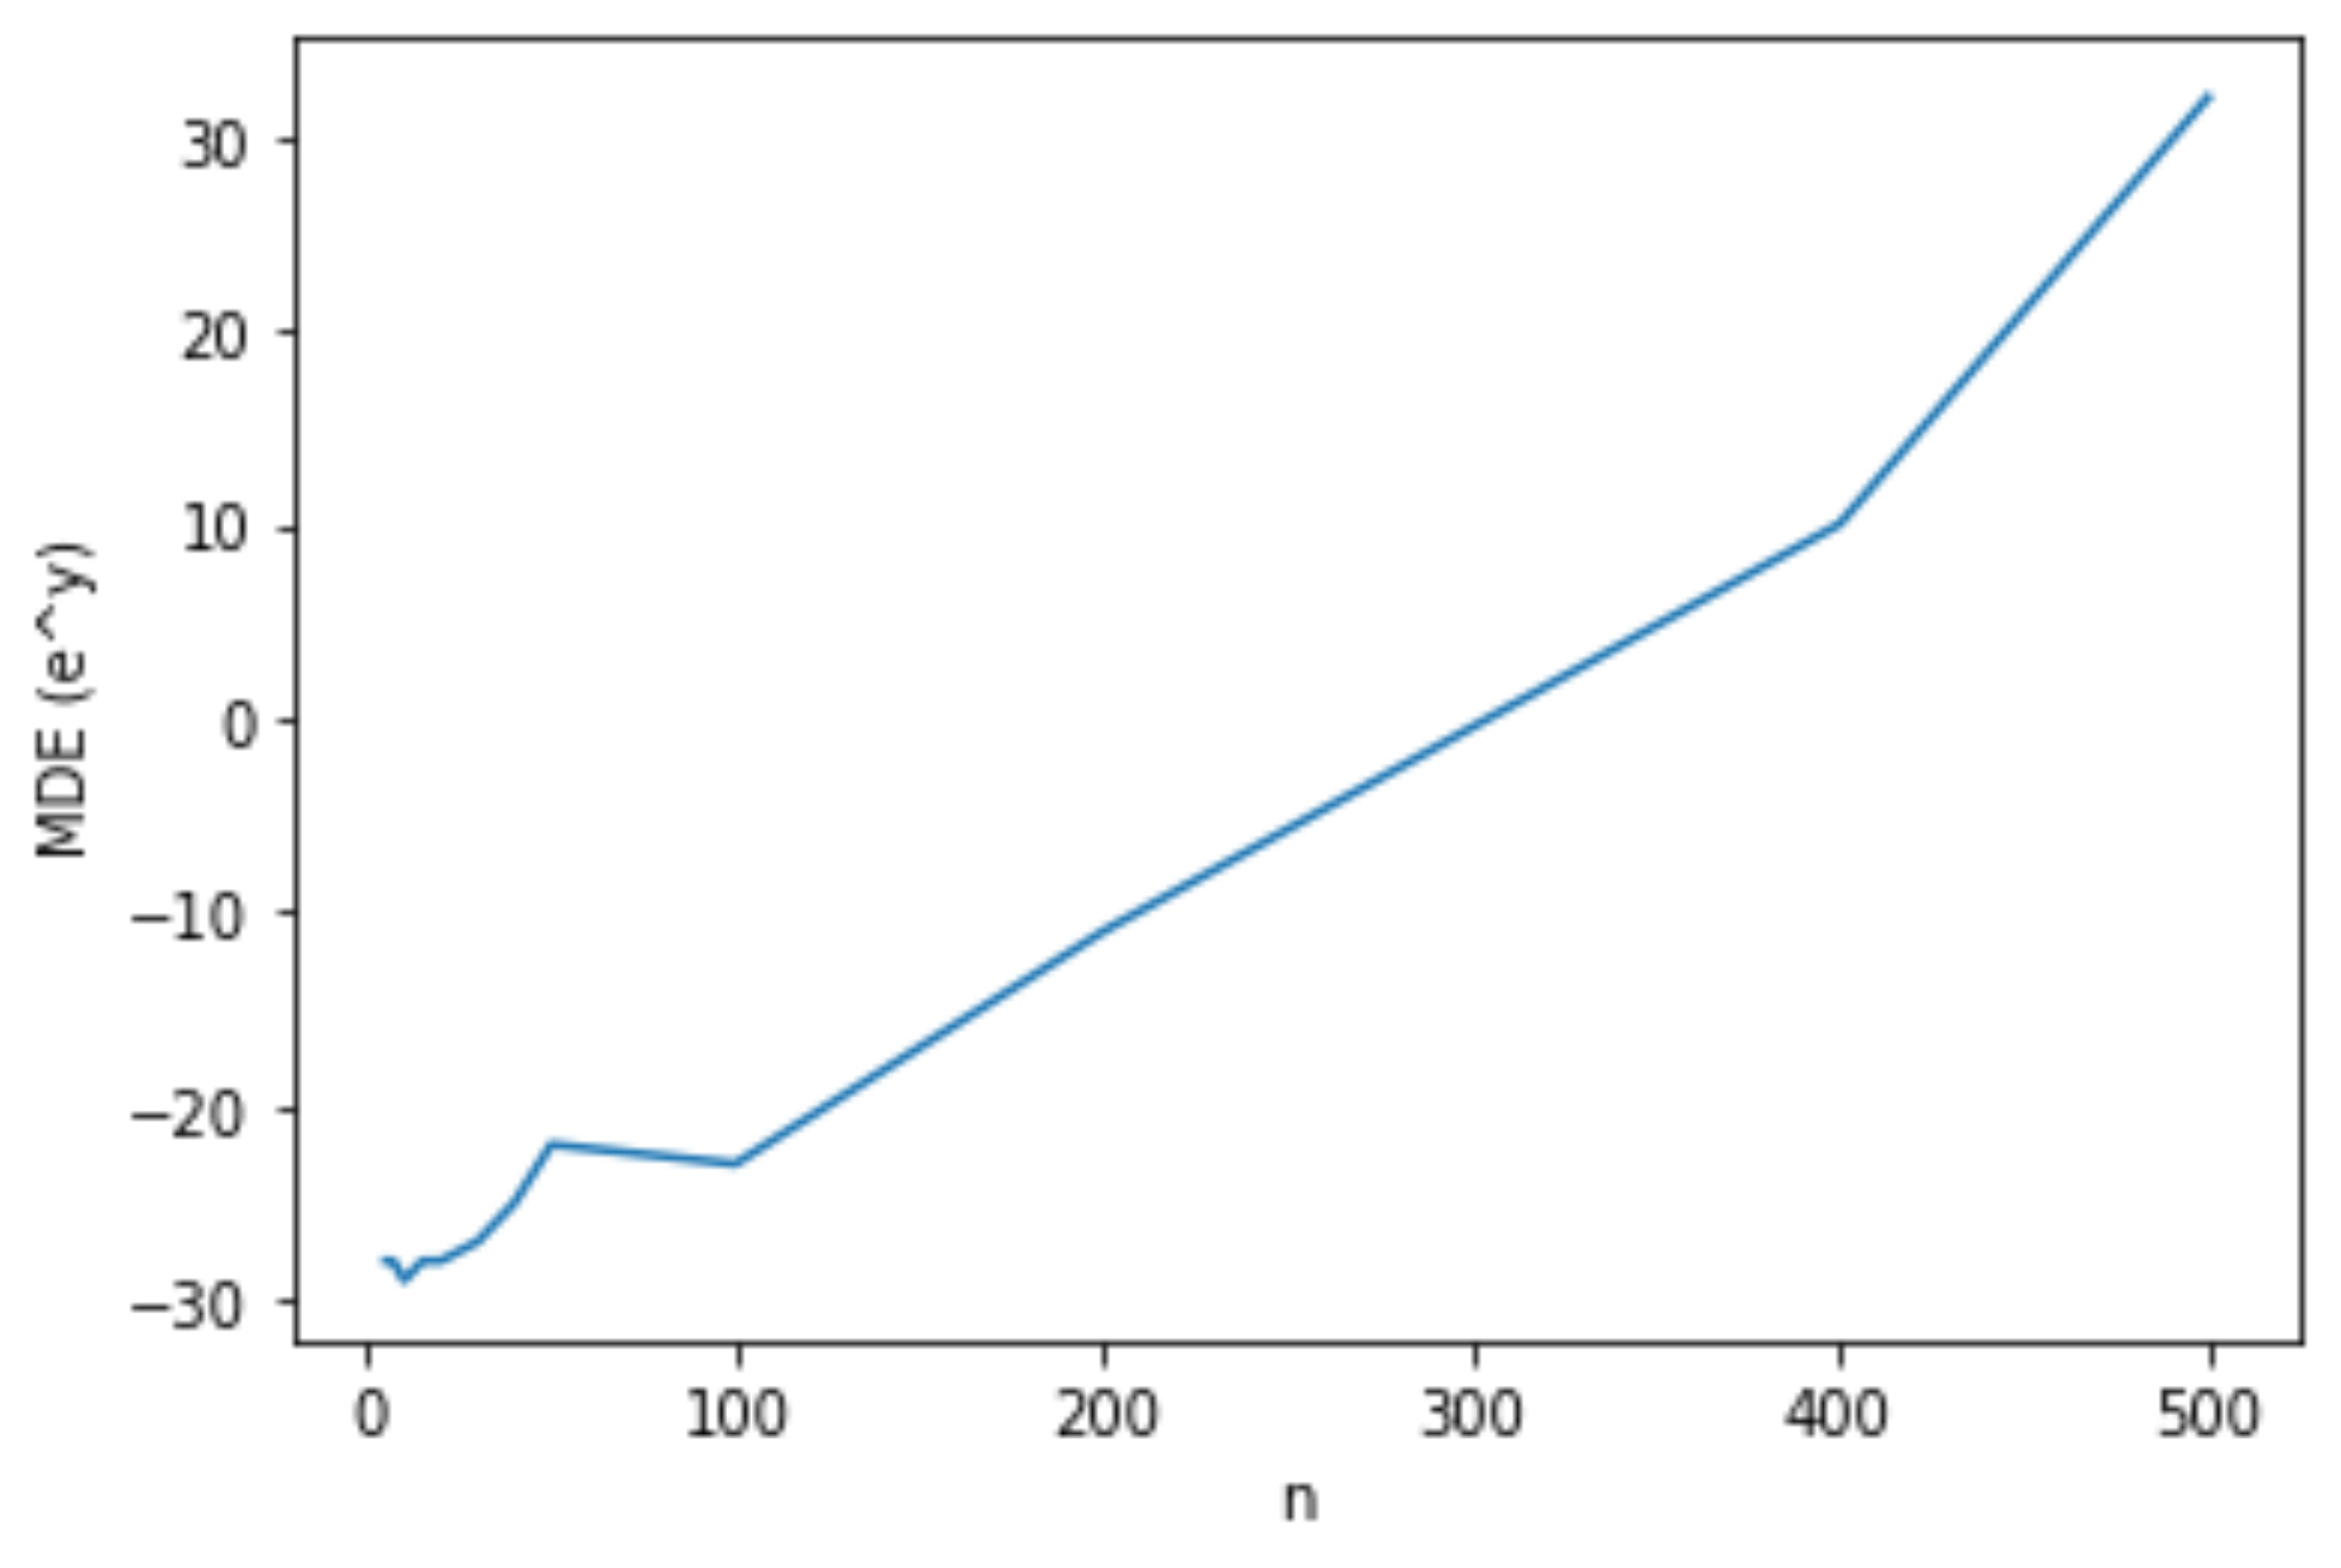
\includegraphics[width=1\linewidth]{figures/mdeTriPro2.png}
					\end{center}
					\label{fig:mdeTri}
				\end{figure}
			\end{minipage}
		\end{center}
		\caption{A esquerda, o tempo de processo e, a direita, a ordem de grandeza associada ao MDE das soluções. Utilizou-se $\mathcal{P} = 0.05$.}
		\label{fig:triPri3}
	\end{figure}
	
	Como esperado, é perceptível uma grande melhora na MDE das soluções conforme se diminui o valor de $\mathcal{P}$. 
	
	Também deve-se perceber que o tempo não obedeceu um padrão perfeito. Podemos relacionar esse fato com a aleatoriedade das instâncias, como pode-se notar que o Algoritmo~\ref{alg:realizacaoTrilateration} teve maios volatilidade no padrão temporal. Mesmo assim, há um consenso. As soluções mostradas nas Figuras~\ref{fig:triPri} e~\ref{fig:triPri3}, por exemplo, demonstram claramente um padrão polinomial, indo de encontro com o que foi apresentado na seção~\ref{sec:oi}.
	
	\newpage
	\section{Considerações Finais}
	Com isso, concluí-se o estudo sobre a Geometria de Distâncias aplicada ao problema de localização de sensores, tal qual teve como resultado um algorítimo que garante encontrar a solução do problema (se houver). .
	\\
	
	Nos cabe, nesse momento, voltarmos atenção às propostas levantadas internamente no início do projeto e verificar se elas foram cumpridas. Seguem o conjunto de objetivos específicos desse projeto, munidos de breve conclusão:
	
	\begin{enumerate}
		
		\item Estudar formas viáveis (pelos vieses energético, de construção e precisão da medida) para obtenção das distâncias entre os elementos do sistema físico:
		
		Fortemente embasado em \cite{savvides2001dynamic} e \cite{sensorsForMobileRobots}, faz-se uma apresentação sobre esses conceitos na Seção~\ref{sec:sensores}. 
		
		\item Estudar as possíveis distribuições dos Robôs Móveis em um sistema genérico, visando verificar quais conjuntos de dados possam ser garantidos como entradas para a construção do problema:
		
		Além de estudar distribuições genéricas, como em \cite{eren2004rigidity}, desenvolve-se na Seção~\ref{sec:disc} o Algorítimo~\ref{alg:instancia}, que cria instâncias aleatórias com diferentes densidades de ligações.
		
		\item Verificar a solução do Discretizable Order Problem \cite{carlileGDandAplications} aplicado ao problema proposto e estudar o ordenamento de vértices que se adeque aos objetivos do trabalho:
		
		Durante o desenvolvimento da Seção~\ref{sec:GD}, percebeu-se que uma ordem de discretização não seria necessária, visto que a definição do problema necessita de uma única solução \cite{libertiEDG}. Por conta disso, definiu-se a ordem de $K$-lateração, que garante a unicidade de solução.
		
		\item Caso consiga-se uma boa ordenação para os vértices, verificar a aplicação do algorítimo Branch-And-Prune \cite{carlile:BP} para a solução do problema proposto. Se não for possível, estudar outros algorítimos que possam solucionar o problema:
		
		Visto que o problema não era discreto, não fora possível aplicar o algorítimo Branch-And-Prune. Ao invés disso, se propôs o Algorítimo~\ref{alg:realizacaoTrilateration}, que utiliza a trilateração como núcleo e garante no máximo uma solução.
		
		\item Estudar a complexidade computacional do algorítimo proposto aplicado as possíveis distribuições:
		
		Isso foi feito no fim das Seções~\ref{sec:GD} e~\ref{sec:disc}, onde verificou-se que o algorítimo pode ser resolvido em tempo polinomial. Também mostrou-se um estudo sobre diferentes visões da geometria do problema afim de minimizar os erros associados. 
		
		\item Simular computacionalmente o algoritmo para solução do problema com instâncias artificialmente geradas, dominando cada passo utilizado:
		
		Simulações apresentadas, de forma satisfatória, na Seção~\ref{sec:disc}.
		
		\item Aplicar o algoritmo estudado em estruturas de pequena escala, como instâncias reais do problema:
		
		Não fora possível cumprir este último objetivo. Infelizmente, a manufatura de robôs móveis usando sensores de distância se demonstrou excessivamente custosa \cite{savvides2001dynamic, sensorsForMobileRobots}.
		
		Vale lembrar, porém, que a utilização de instâncias artificiais genéricas se mostrou de grande importância. Pode-se averiguar e discutir sobre diferentes geometrias, mesmo sem a prototipação de fato.
		
	\end{enumerate}
	
	Como experiências futuras, deseja-se estudar mais sobre a obtenção e tratamento de dados de distâncias, visto que esses possuem erros de medida \cite{sensorsForMobileRobots} (não levados em consideração nesse trabalho). Alguns trabalhos relacionados à Geometria de Distâncias aplicada ao caso intervalar são mostrados em \cite{wsnlSemidefinitePrograming}. Há curiosidade em ver como medida MDE se comporta para uma quantidade grande de vértices associados a erros de medida.
	
	Também deseja-se fazer estudos sobre geometrias mínimas para o problema, como feito em \cite{wsnlFewAnchors}. Deseja-se verificar um conjunto de condições que restringem o movimento de um robô móvel afim de garantir que este ainda possa ser localizado.
	
	\newpage
	\phantomsection
	\addcontentsline{toc}{section}{Referências}
	
	\bibliographystyle{unsrt}
	\bibliography{references}
	
	\newpage
	\appendix
	\input{secGD/apendices.tex}

\end{document}

	
	\newpage
	
	 \documentclass[a4paper,12pt]{article}
\usepackage[a4paper,top=3cm,bottom=2cm,left=3cm,right=3cm,marginparwidth=1.75cm]{geometry}
\usepackage[brazil]{babel}
\usepackage[T1]{fontenc}
\usepackage[utf8]{inputenc}
\usepackage{amsmath}
\usepackage{MnSymbol}
\usepackage{wasysym}
\usepackage{hyperref}
\usepackage{color}
\definecolor{Blue}{rgb}{0,0,0.9}
\definecolor{Red}{rgb}{0.9,0,0}
\usepackage{esvect}
\usepackage{graphicx}
\usepackage{float}
\usepackage{indentfirst}
\usepackage{caption}
\usepackage{blkarray}
\newcommand\Mark[1]{\textsuperscript#1}
\usepackage{pgfplots}
\usepackage{amsfonts}
\usepackage[english, ruled, linesnumbered]{algorithm2e}
\usepackage{algorithmic}
\newtheorem{definicao}{Definição}[section]
\newtheorem{teorema}{Teorema}[section]

\title{Disposição de Robôs Móveis no espaço Euclidiano 3D: uma aplicação de Geometria de Distâncias}
\author{Guilherme Philippi\Mark{*}, orientado por Felipe Delfini Caetano Fidalgo\Mark{\dagger}\\Campus Blumenau\\Universidade Federal de Santa Catarina\\UFSC
	\\guilherme.philippi@grad.ufsc.br\Mark{*}, felipe.fidalgo@ufsc.br\Mark{\dagger}}
\begin{document}
	\begin{titlepage}
		\newcommand{\HRule}{\rule{\linewidth}{0.5mm}} % Defines a new command for the horizontal lines, change thickness here
		\center % Center everything on the page
		%----------------------------------------------------------------------------------------
		%	HEADING SECTIONS
		%----------------------------------------------------------------------------------------
		\begin{center}
			
\includegraphics[scale=0.22]{figures/logoufsc.jpg}
		\end{center}
		\vspace{1cm}
		
		\textsc{\LARGE \hspace{-0.17cm}Universidade Federal de Santa Catarina}\\[0.5cm] % Name of your university/college
		{\Large Centro de Blumenau \\ Departamento de Matemática}\\[1.5cm] % Major heading such as course name
		\textsc{\Large PIBIC \\ Relatório Final \vspace{1.5cm}  \\ }{\large Geometria de Distâncias e Álgebras Geométricas: novas perspectivas geométricas, computacionais e aplicações}\\[2.0cm] % Minor heading such as course title
		
		%\textsc{\LARGE Universidade Federal de Santa Catarina}\\[0.5cm] % Name of your university/college
		%{\Large Centro de Blumenau \\ Departamento de Matemática}\\[1.5cm] % Major heading such as course name
		%\textsc{\Large PIBIC \\ Programa Institucional de Bolsas de Iniciação Científica \vspace{1.5cm} \\ {\bf PROJETO DE PESQUISA}}\\[2.0cm] % Minor heading such as course title
		
		%----------------------------------------------------------------------------------------
		%	TITLE SECTION
		%----------------------------------------------------------------------------------------
		
		\HRule \\[0.4cm]
		{ \LARGE \bfseries \textbf{Disposição de Robôs Móveis no espaço Euclidiano 3D: uma aplicação de Geometria de Distâncias}} \\ [0.4cm] % Title of your document
		\HRule \\[2cm]
		
		%----------------------------------------------------------------------------------------
		%	AUTHOR SECTION
		%----------------------------------------------------------------------------------------
		
		\begin{minipage}{1\textwidth}
			\begin{center} \large
				Guilherme Philippi (g.philippi@grad.ufsc.br),
				\vspace{0.5cm}
				\\
				\underline{\textsc{Orientador:}} \vspace{0.2cm}
				Felipe Delfini Caetano Fidalgo (felipe.fidalgo@ufsc.br).
			\end{center}
		\end{minipage} \\[2cm]
		
		
		{\large \today} % Date, change the \today to a set date if you want to be precise
		
		
		\vfill % Fill the rest of the page with whitespace
		
	\end{titlepage}
	
	
	\newpage
	\vspace{-1cm}
	\tableofcontents
	\newpage
	
	\begin{center}
		\large
		\textbf{Abstract}
	\end{center}
	
	
	In this work, the Distance Geometry Problem Trilaterative applied to the sensor location problem was studied, as well as the necessary tools for its understanding, going from graph theory to the characteristics of systems involving mobile robotics. An overview of Geometry of Distances was presented, which enabled the correct definition of the problem and polynomial algorithms to solve it. The text ends with an analysis of computer simulations of the problem, using different geometries, as well as an algorithm to generate them.
	
	\textbf{Keywords:} TDGP, Distance Geometry, Mobile Robotics.
	
	
	\vspace{2cm}	
	\begin{center}
		\large
		\textbf{Resumo}
	\end{center}
	
	Neste trabalho, foram estudados o Trilaterativo Distance Geometry Problem aplicado ao problema de localização de sensores, bem como as ferramentas necessárias para sua compreensão, passando da teoria de grafos às características de sistemas envolvendo robótica móvel. Apresentou-se uma visão geral de Geometria de Distâncias que possibilitou a correta definição do problema e de algorítimos polinomiais para solucioná-lo. O texto se encerra com uma analise de simulações computacionais do problema, utilizando diferentes geometrias, bem como um algorítimo para gerá-las. 
	
	\textbf{Palavras-chave:} TDGP, Geometria de Distâncias, Robótica Móvel.
	
	
	\newpage
	\section{Introdução}
	
	Percebe-se uma tendencia de mercado em se adotar sistemas autônomos móveis para realizar funções que dependem de um grande número de maquinas, como o controle do estoque em um armazém, um sistema de entrega ou o cultivo e tratamento de grandes áreas de plantio \cite{mobileRobotsCook}. O estudo da localização de robôs móveis é vasta na literatura \cite{eren2004rigidity, mobileRobotsTzafestas}, o que demonstra a importância deste tema. Qualquer solução de engenharia móvel, seja autônoma ou não, precisa definir uma forma de localizar seu objeto de estudo. Por conta disso, ao decorrer desse texto apresenta-se soluções envolvendo Geometria de Distâncias como alternativas para a obtenção de localização.
	\\
	
	A Geometria de Distâncias (GD) é uma matéria de interesse relativamente recente da Ciência \cite{carlileGDandAplications}, disposta em uma vasta interseção entre diversas áreas do conhecimento. Em suma, ela se preocupa com os aspectos geométricos decorrentes dos objetos que estão dispostos em algum espaço e possuam uma relação de distância medível, advindas de origens tão variáveis quanto se queira. Como é o caso de estudo deste texto: distâncias entre robôs móveis com seu meio e, em particular, outros robôs móveis.
	\\
	
	Para poder relacionar esses distâncias, no que se segue, apresenta-se um estudo sobre a Teoria de Grafos (Seção~\ref{sec:grafos}), que demonstrou-se uma ferramenta importante para GD --- em contraponto à antiga utilização de matrizes de distâncias \cite{carlileGDandAplications}. A seguir, por tanto, na Seção~\ref{sec:GD}, desenvolve-se o problema fundamental deste trabalho a partir da definição de Grafos e faz-se um estudo sobre algorítimos descritos na literatura para solucioná-lo. Na Seção~\ref{sec:robos}, faz-se uma introdução a robótica móvel e apresenta-se um estudo sobre sensoriamento. 
	
	O trabalho se encerra com algumas simulações computacionais do problema, na Seção~\ref{sec:disc}, além de discussões envolvendo esses resultados. O texto também contém dois apêndices, podendo serem usados como consulta, caracterizando algumas ferramentas matemáticas utilizadas. 
	\\
	
	A revisão bibliográfica completa pode ser encontrada no fim do documento, sendo devidamente citada durante o texto. 
	
	\newpage
	
	\phantomsection
	\addcontentsline{toc}{section}{Materiais e Métodos}
	\section*{Materiais e Métodos}
	No que se segue, apresenta-se o estudo desenvolvido neste trabalho.
	
	\input{secGrafos/gphilippi.tex}
	
	\newpage
	
	\input{secGD/gphilippi.tex}
	
	\newpage
	
	\input{secRobosMoveis/gphilippi.tex}

	\newpage
	\section{Resultados e Discussão \label{sec:disc}}
	Afim de ilustrar e averiguar a eficiência do que foi apresentado aqui, realizou-se algumas simulações computacionais implementando os Algorítimos~\ref{alg:realizacaoIterativa} e~\ref{alg:realizacaoTrilateration} em C. 
	\\
	
	Tais simulações foram executadas em um computador pessoal utilizando o sistema operacional Manjaro (uma distribuição Linux baseada em Arch), equipado com um processador Intel Core i5-8600K (6 núcleos operando em 4.1Ghz) e um pente de memória DDR4 2666MHz de 8Gb em \textit{Single-Channel} (operando, por tanto, em 1333Mhz).	
	\\
	
	Para a eficiência dos algorítimos, fez-se uso da biblioteca de código aberto LAPACKE, que é uma interface para o LAPACK (\textit{Linear Algebra Packge}) em C, onde encontra-se algumas implementações muito otimizadas de operações elementares envolvendo Álgebra Linear. Por exemplo, possui funções para solucionar sistemas matriz-vetor $Ax = b$, através da decomposição matricial LU \cite{AlgebraLinearElon}, que pôde ser usada para solucionar o sistema linear~\ref{eq:DGPLinearSystem}, discutido na seção~\ref{sec:trilateration}.
	
	\subsection{Erro acumulado}
	
	Como tanto o algorítimo~\ref{alg:realizacaoIterativa} quanto o~\ref{alg:realizacaoTrilateration} calculam posições em função de realizações previamente calculadas, é inevitável o acumulo de erros entre essas realizações. Mesmo que a solução teórica seja perfeita, na prática os valores não são representados exatamente. Isso se dá pois o computador não trabalha no conjunto dos números reais, ou, pior, para qualquer $i \in\mathbb{R}$, a possibilidade de $i$ não pode ser representado pelo computador tem probabilidade 1. Por isso, gera-se a necessidade de analisar o quão perto as soluções calculadas estão das reais.
	
	Neste texto, a principal medida de confiabilidade de uma solução será calculada através da \textit{Mean Distance Error}, como segue \cite{mucherino:BP}.
	
	\begin{center}
		\begin{minipage}{0.9 \linewidth}
			\textbf{\textit{Mean Distance Error} (MDE)}: Seja $G= (V,E,d)$ um grafo ponderado que defina uma instância DGP. Se $\{x_1, \dots, x_n\}$ é um conjunto que define uma realização dos $n$ vértices de $G$ e então,
			$$MDE(x) = \frac{1}{|d\;|} \sum_{i,j}^{}\frac{|||x_i - x_j|| - d_{i,j}|}{d_{i,j}} .$$
		\end{minipage}
	\end{center}
	
	\subsection{Exemplares utilizados}
	Como entrada das simulações, implementou-se o Algorítimo~\ref{alg:instancia}, que gera um grafo $K$-laterativo com $n$ vértices de coordenadas aleatórias $x_i = (x_{i1},\dots,x_{iK})\in \mathbb{R}^K$ e provê um conjunto limitável de arestas. Esse limitação é definida pelo parâmetro $\mathcal{P} \in [0,1]$, como coeficiente de probabilidade de uma aresta ser ou não acessível entre dois vértices aleatório $v_i$ e $v_j$, com $i,j>K+1$ (garantindo que sempre haverá ao menos uma (K+1)-clique adjacente a todo vértice).
	\\
	
	\begin{algorithm}[H]
		\label{alg:instancia}
		\tcp{Percorra todos os vértices}
		\For{$i\in \{0,\dots,n\}$}{
			\tcp{Varie entre cada coordenada de $x_i\in\mathbb{R}^K$}
			\For{$j \in {1,\dots,K}$}{
				\tcc{Atribua um valor aleatório para cada co. A função Aleatorio(\textit{m}) gera valores entre 0 e \textit{m}.}
				$x_{ij} = $Aleatorio$(m)$; 
			}
		}
		\tcp{Para cada vértice, percorra todos os seus antecessores}
		\For{$x_i \in \{x_n, \dots,x_1\}$}{
			\For{$x_j \in \{x_1, \dots,x_{i-1}\}$}{
				\tcp{Gere um número $a \in [0,1]$ aleatório.}
				Seja $a$ = Aleatorio(1);
				
				\tcp{Verifique se $a > \mathcal{P}$ e se $i,j > K$}
				\If{$a > \mathcal{P}$ and $i > K$ and $j>K$}{
					\tcp{Defina uma aresta entre $x_i$ e $x_j$}
					$e_{i,j} = \|x_i - x_j\|$;
				}
			}
		}
		\textbf{return} $G = (\{v_1,\dots,v_n\}, \{\{e_{1,2}\}, \dots,\{e_{j}\}\})$;
		\caption{$G =$ criaInstancia$(n, \mathcal{P})$}
	\end{algorithm}
	\vspace{0.4cm}
	
	Por exemplo, com o Algorítimo~\ref{alg:instancia} gerou-se a instância mostrada ma Figura~\ref{fig:inst}.
	
	\begin{figure}[H]
	\begin{center}
		\begin{minipage}{0.15 \linewidth}
			\begin{table}[H]
				\centering
				\begin{tabular}{ |c c c| } 
					\hline
					\textbf{x} & \textbf{y} & \textbf{z} \\\hline
					(33, & 36, & 27)\\

					(15, & 43, & 35)\\

					(36, & 42, & 49)\\

					(21, & 12, & 27)\\

					(40, & 9, & 13)\\\hline

				\end{tabular}
				\label{tab:re1}
			\end{table}
		\end{minipage}
	\hspace{0.1cm}
		\begin{minipage}{0.8 \linewidth}
			$$
			\begin{bmatrix}
			 0.000000 & 20.904545 & 23.000000 & 26.832816 & 31.208973\\

			20.904545 & 0.000000 & 25.258662 & 32.572995 & 47.592016\\

			23.000000 & 25.258662 & 0.000000 & 40.112342 & 49.000000\\

			26.832816 & 32.572995 & 40.112342 & 0.000000 & 23.790755\\

			31.208973 & 47.592016 & 49.000000 & 23.790755 & 0.000000	
			\end{bmatrix}
			$$
		\end{minipage}
	\end{center}
\caption{A esquerda, as coordenadas dos vértices gerados e, a direita, a matriz de distância a eles associados.}
\label{fig:inst}
\end{figure}
	
	\subsection{Simulações}
	
	Primeiramente. para gerar instâncias do algorítimo~\ref{alg:realizacaoIterativa}, deve-se usar o algorítimo~\ref{alg:instancia} com $\mathcal{P} = 100$. Assim pode-se garantir a geração de um grafo completo. Criou-se, então, instâncias com tamanhos variados: $n \in \{5, 6, 7,10,15,20,30,40,50,100,200,400,500\}$. A seguir apresenta-se alguns gráficos sobre os resultados.
	
	\begin{figure}[H]
		\begin{center}
			\begin{minipage}{0.45 \linewidth}
				\begin{figure}[H]
					\begin{center}
						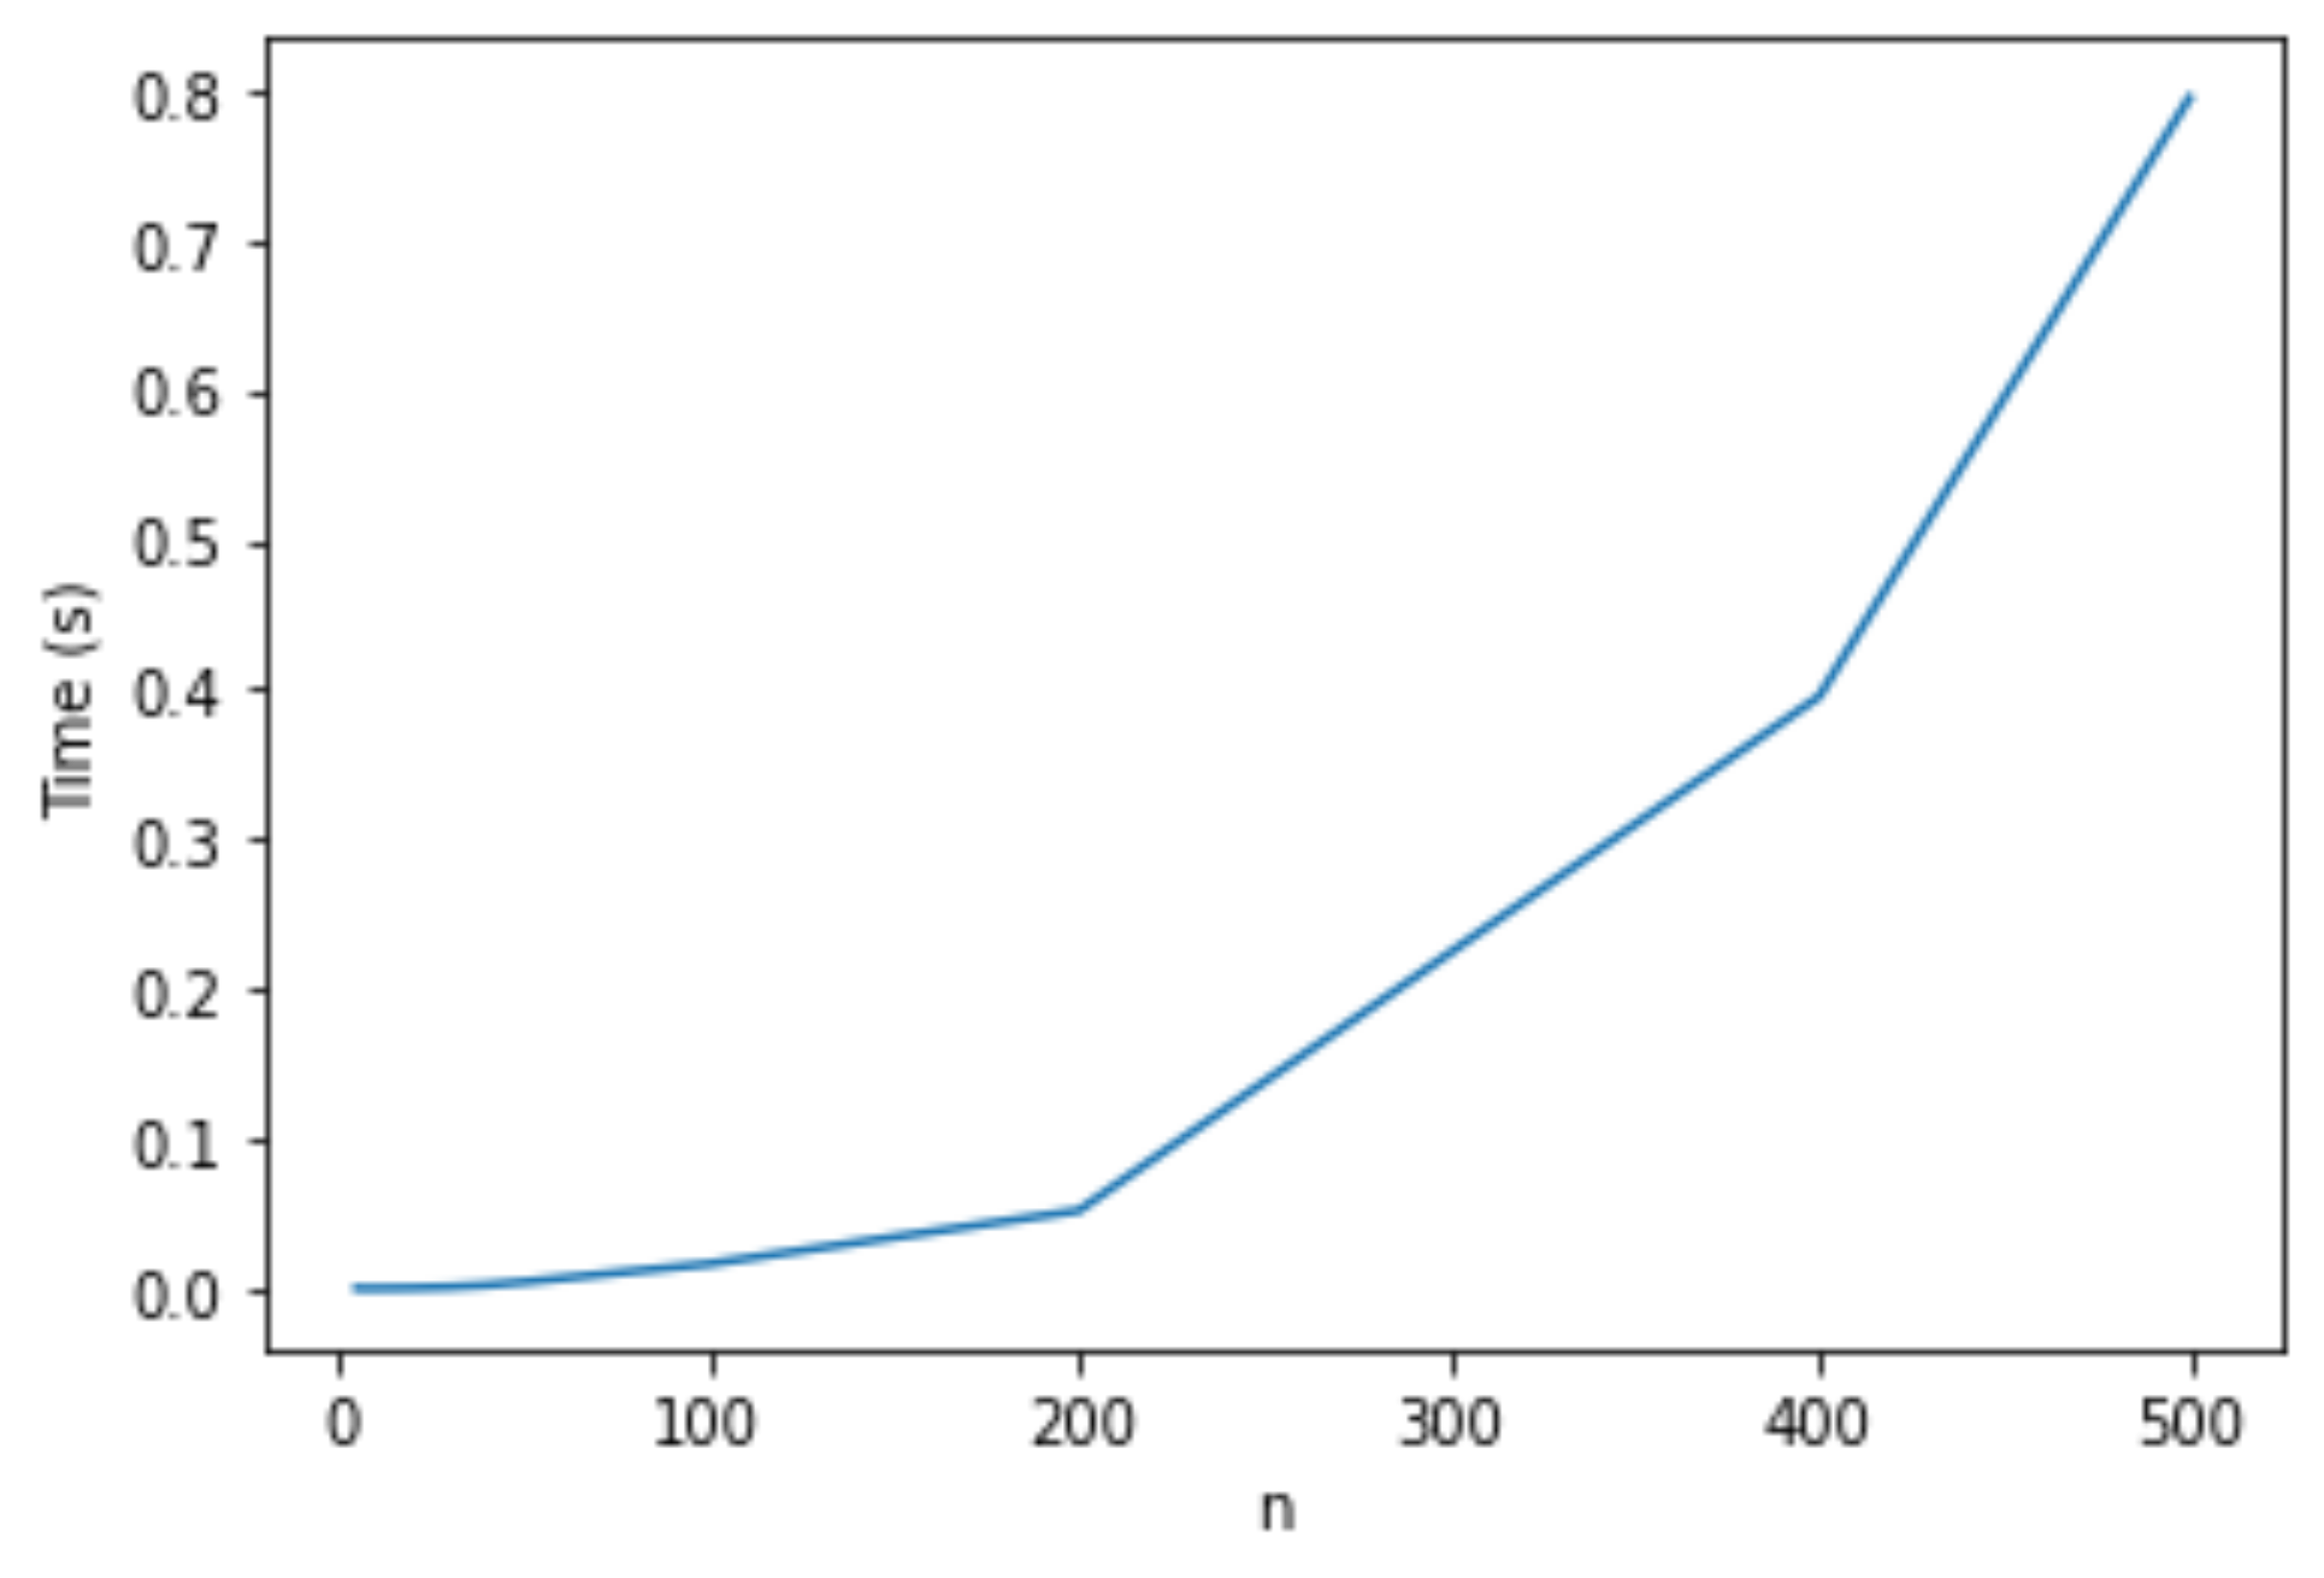
\includegraphics[width=1\linewidth]{figures/tempoTri.png}
					\end{center}
				\end{figure}
			\end{minipage}
			\hspace{0.1cm}
			\begin{minipage}{0.45 \linewidth}
				
				\begin{figure}[H]
					\begin{center}
						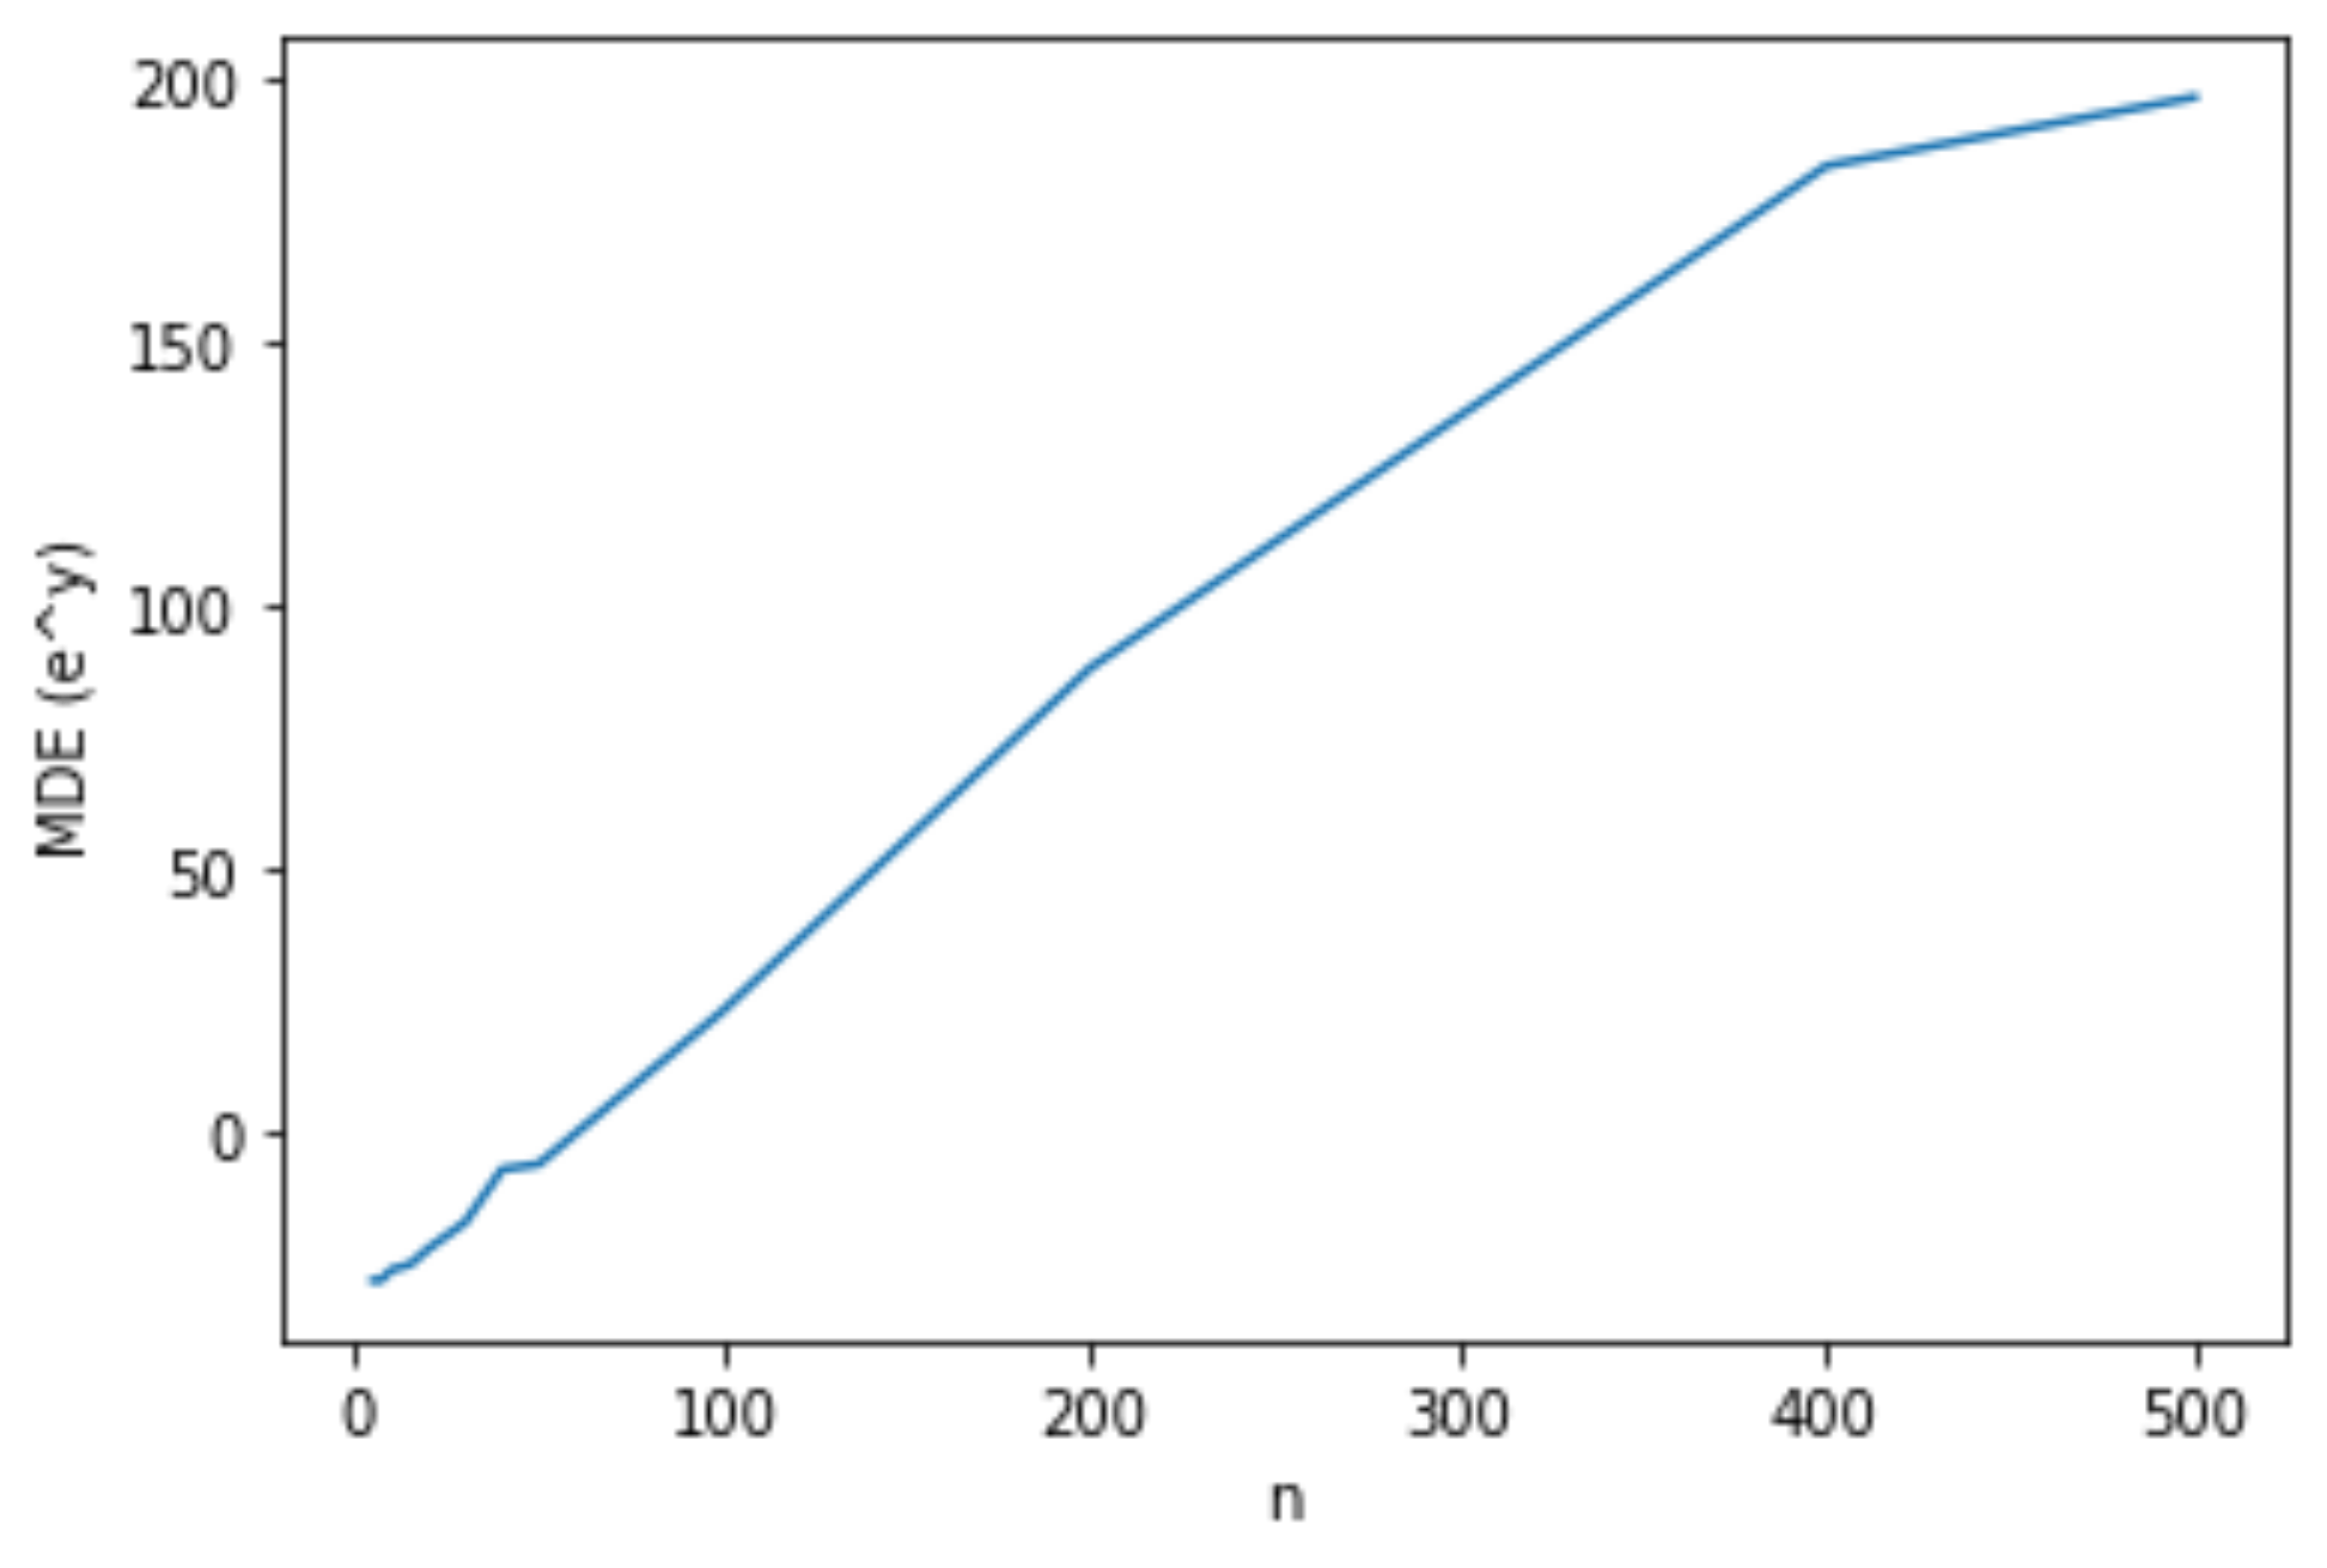
\includegraphics[width=1\linewidth]{figures/mdeTri.png}
					\end{center}
				\end{figure}
			\end{minipage}
		\end{center}
		\caption{A esquerda, o tempo de processo e, a direita, a ordem de grandeza associada ao MDE das soluções.}
		\label{fig:tri}
	\end{figure}
	
	Perceba o comportamento mostrado na Figura~\ref{fig:tri}. Teve-se que fazer uma linearização no gráfico que representa o MDE da solução, pois este cresceu exponencialmente e foi para a ordem de $10^{200}$ em 500 vértices. Esse comportamento se deu por conta dos erros acumulados entre as iterações.
	\\
	
	Uma proposta pensada para contornar essa situação infeliz foi alterar o valor de $\mathcal{P}$, deixando o menor, obrigando o algorítimo a calcular realizações utilizando vértices iniciais. Porém, isso implicaria em um grafo não completo, o que não condiz definição do Algorítimo~\ref{alg:realizacaoIterativa}.
	
	Outra solução proposta fora de utilizar sempre os primeiros vértices no lugar dos antecessores mais próximos. Isso significaria utilizar sempre os vértices âncoras para realizar os demais, semelhante com o que é feito no sistema GPS. Com isso, tivemos os resultados satisfatórios apresentados pela Figura~\ref{fig:triPri}. Perceba que mesmo com 500 vértices ainda obteve-se resultados com $MDE$ na ordem de $10^{-20}$.
	
	\begin{figure}[H]
		\begin{center}
			\begin{minipage}{0.45 \linewidth}
				\begin{figure}[H]
					\begin{center}
						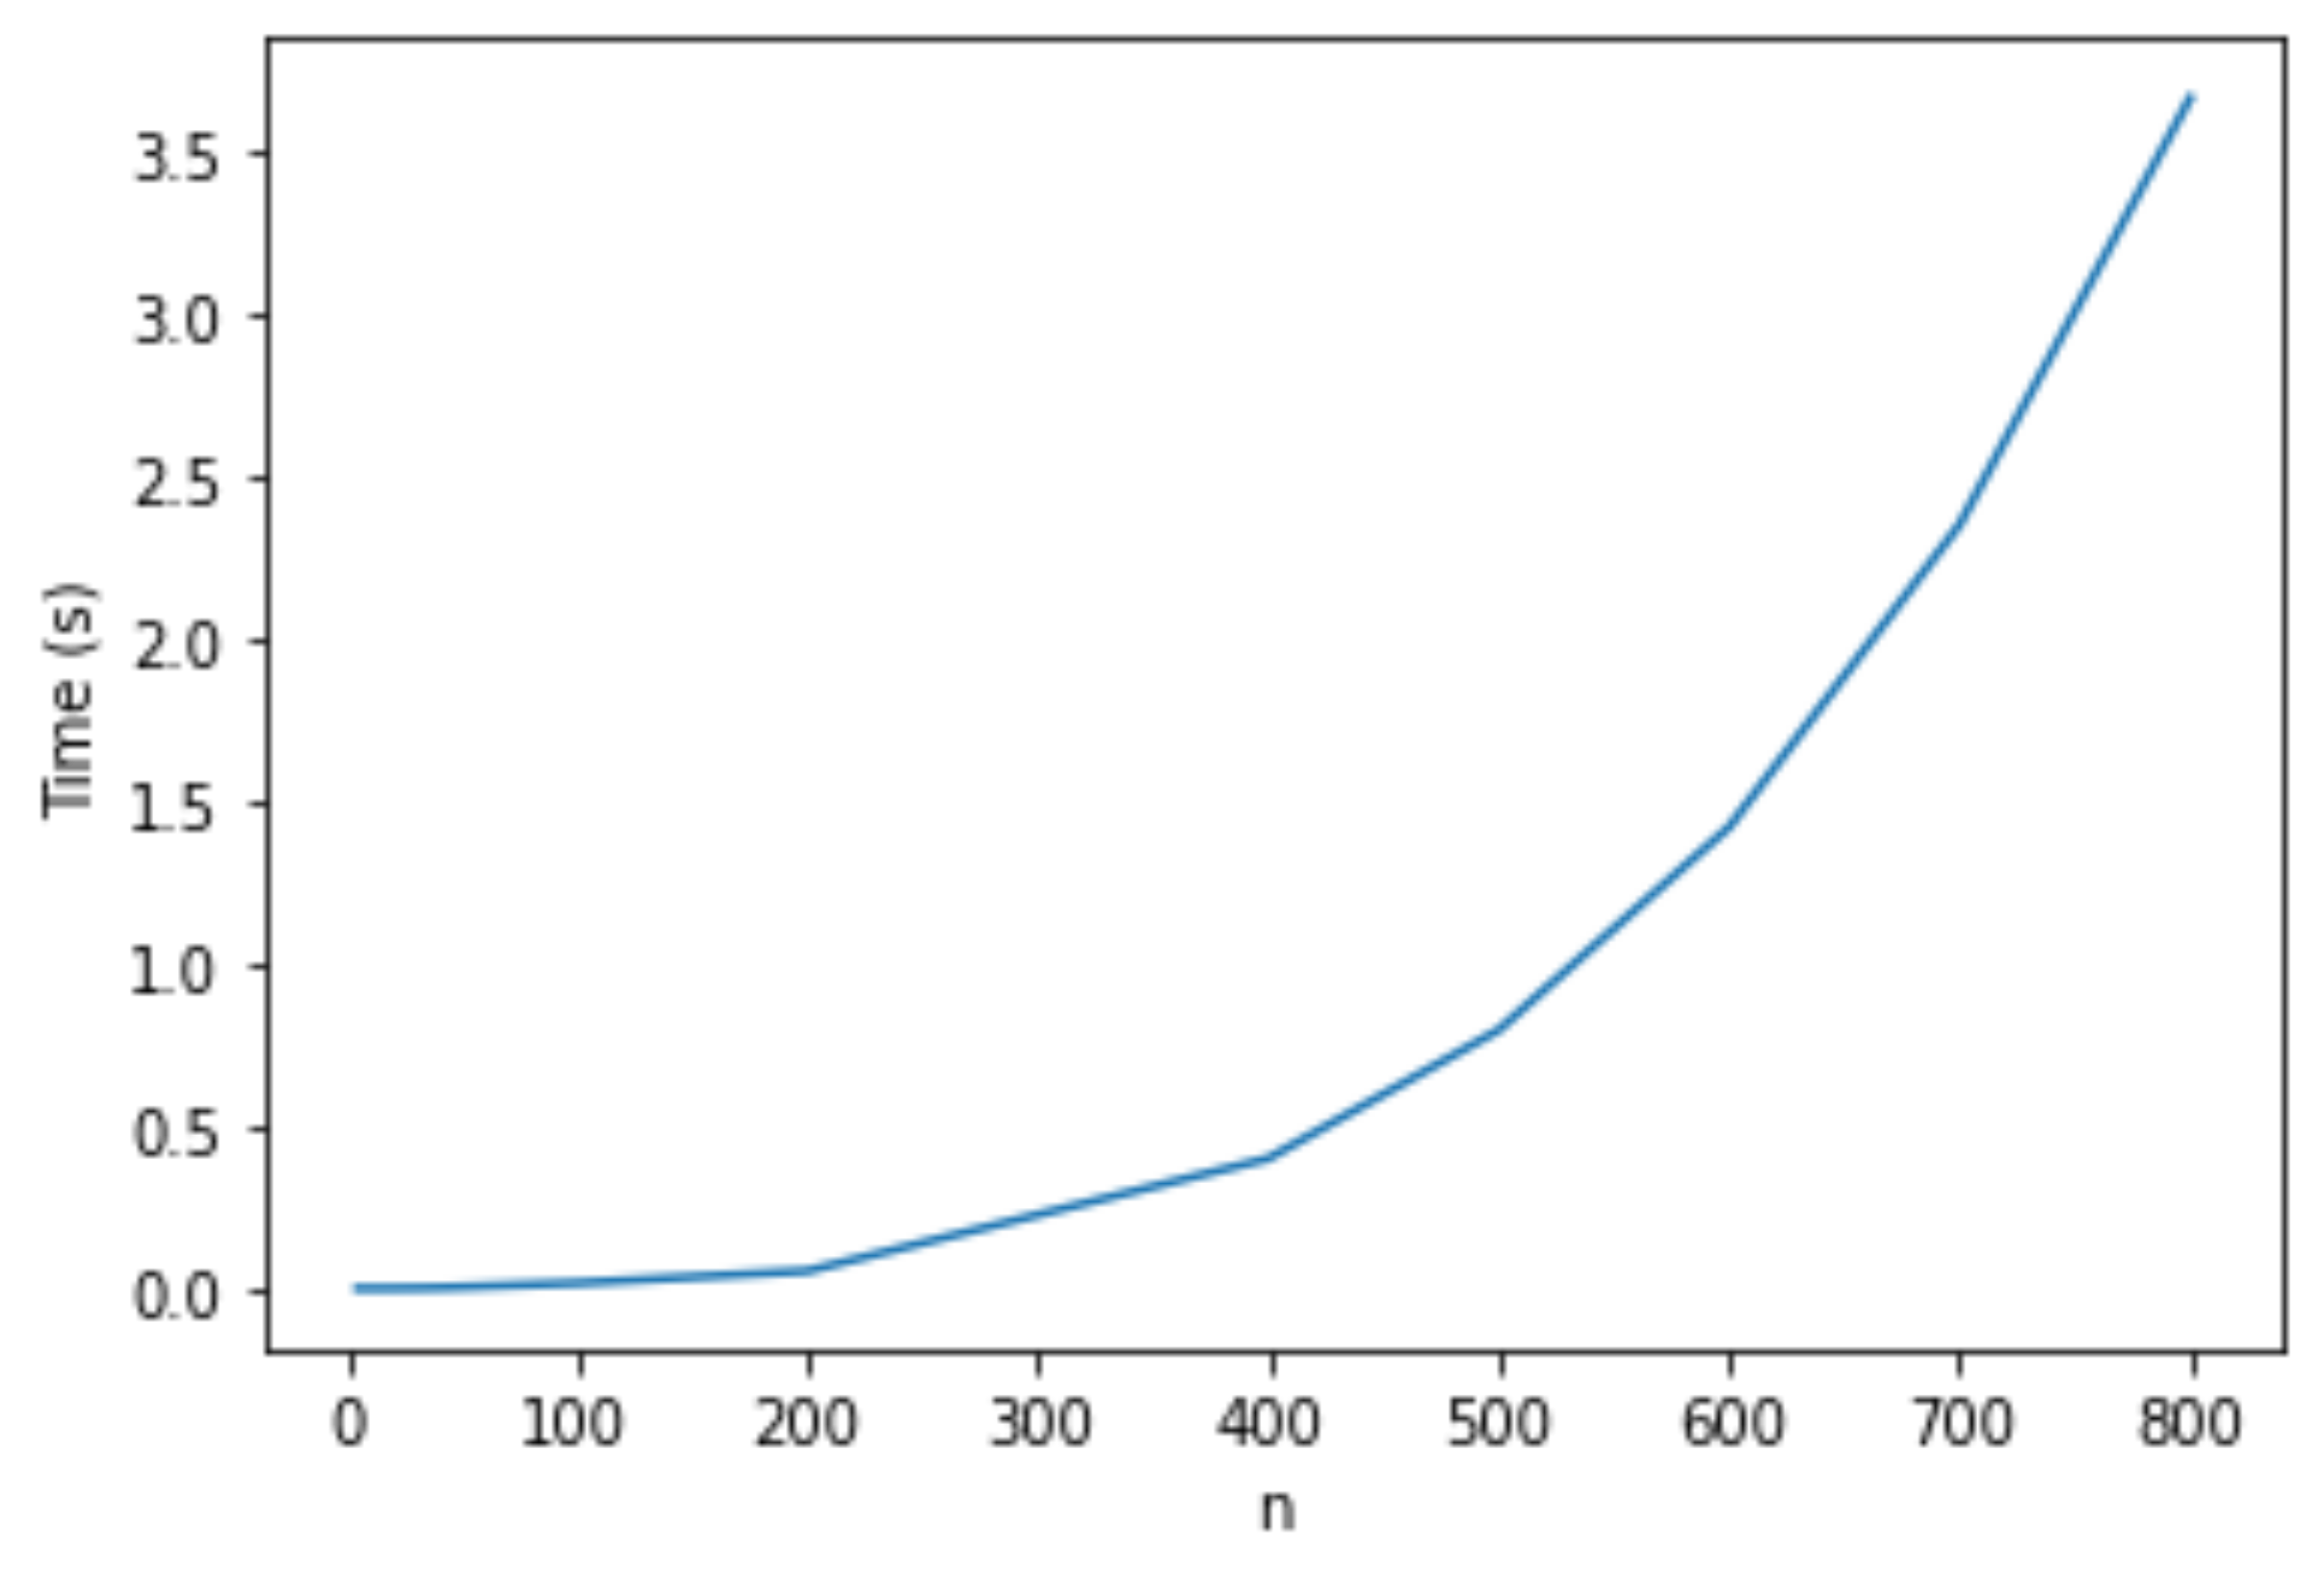
\includegraphics[width=1\linewidth]{figures/tempoTriPri.png}
					\end{center}
				\end{figure}
			\end{minipage}
			\hspace{0.1cm}
			\begin{minipage}{0.45 \linewidth}
				
				\begin{figure}[H]
					\begin{center}
						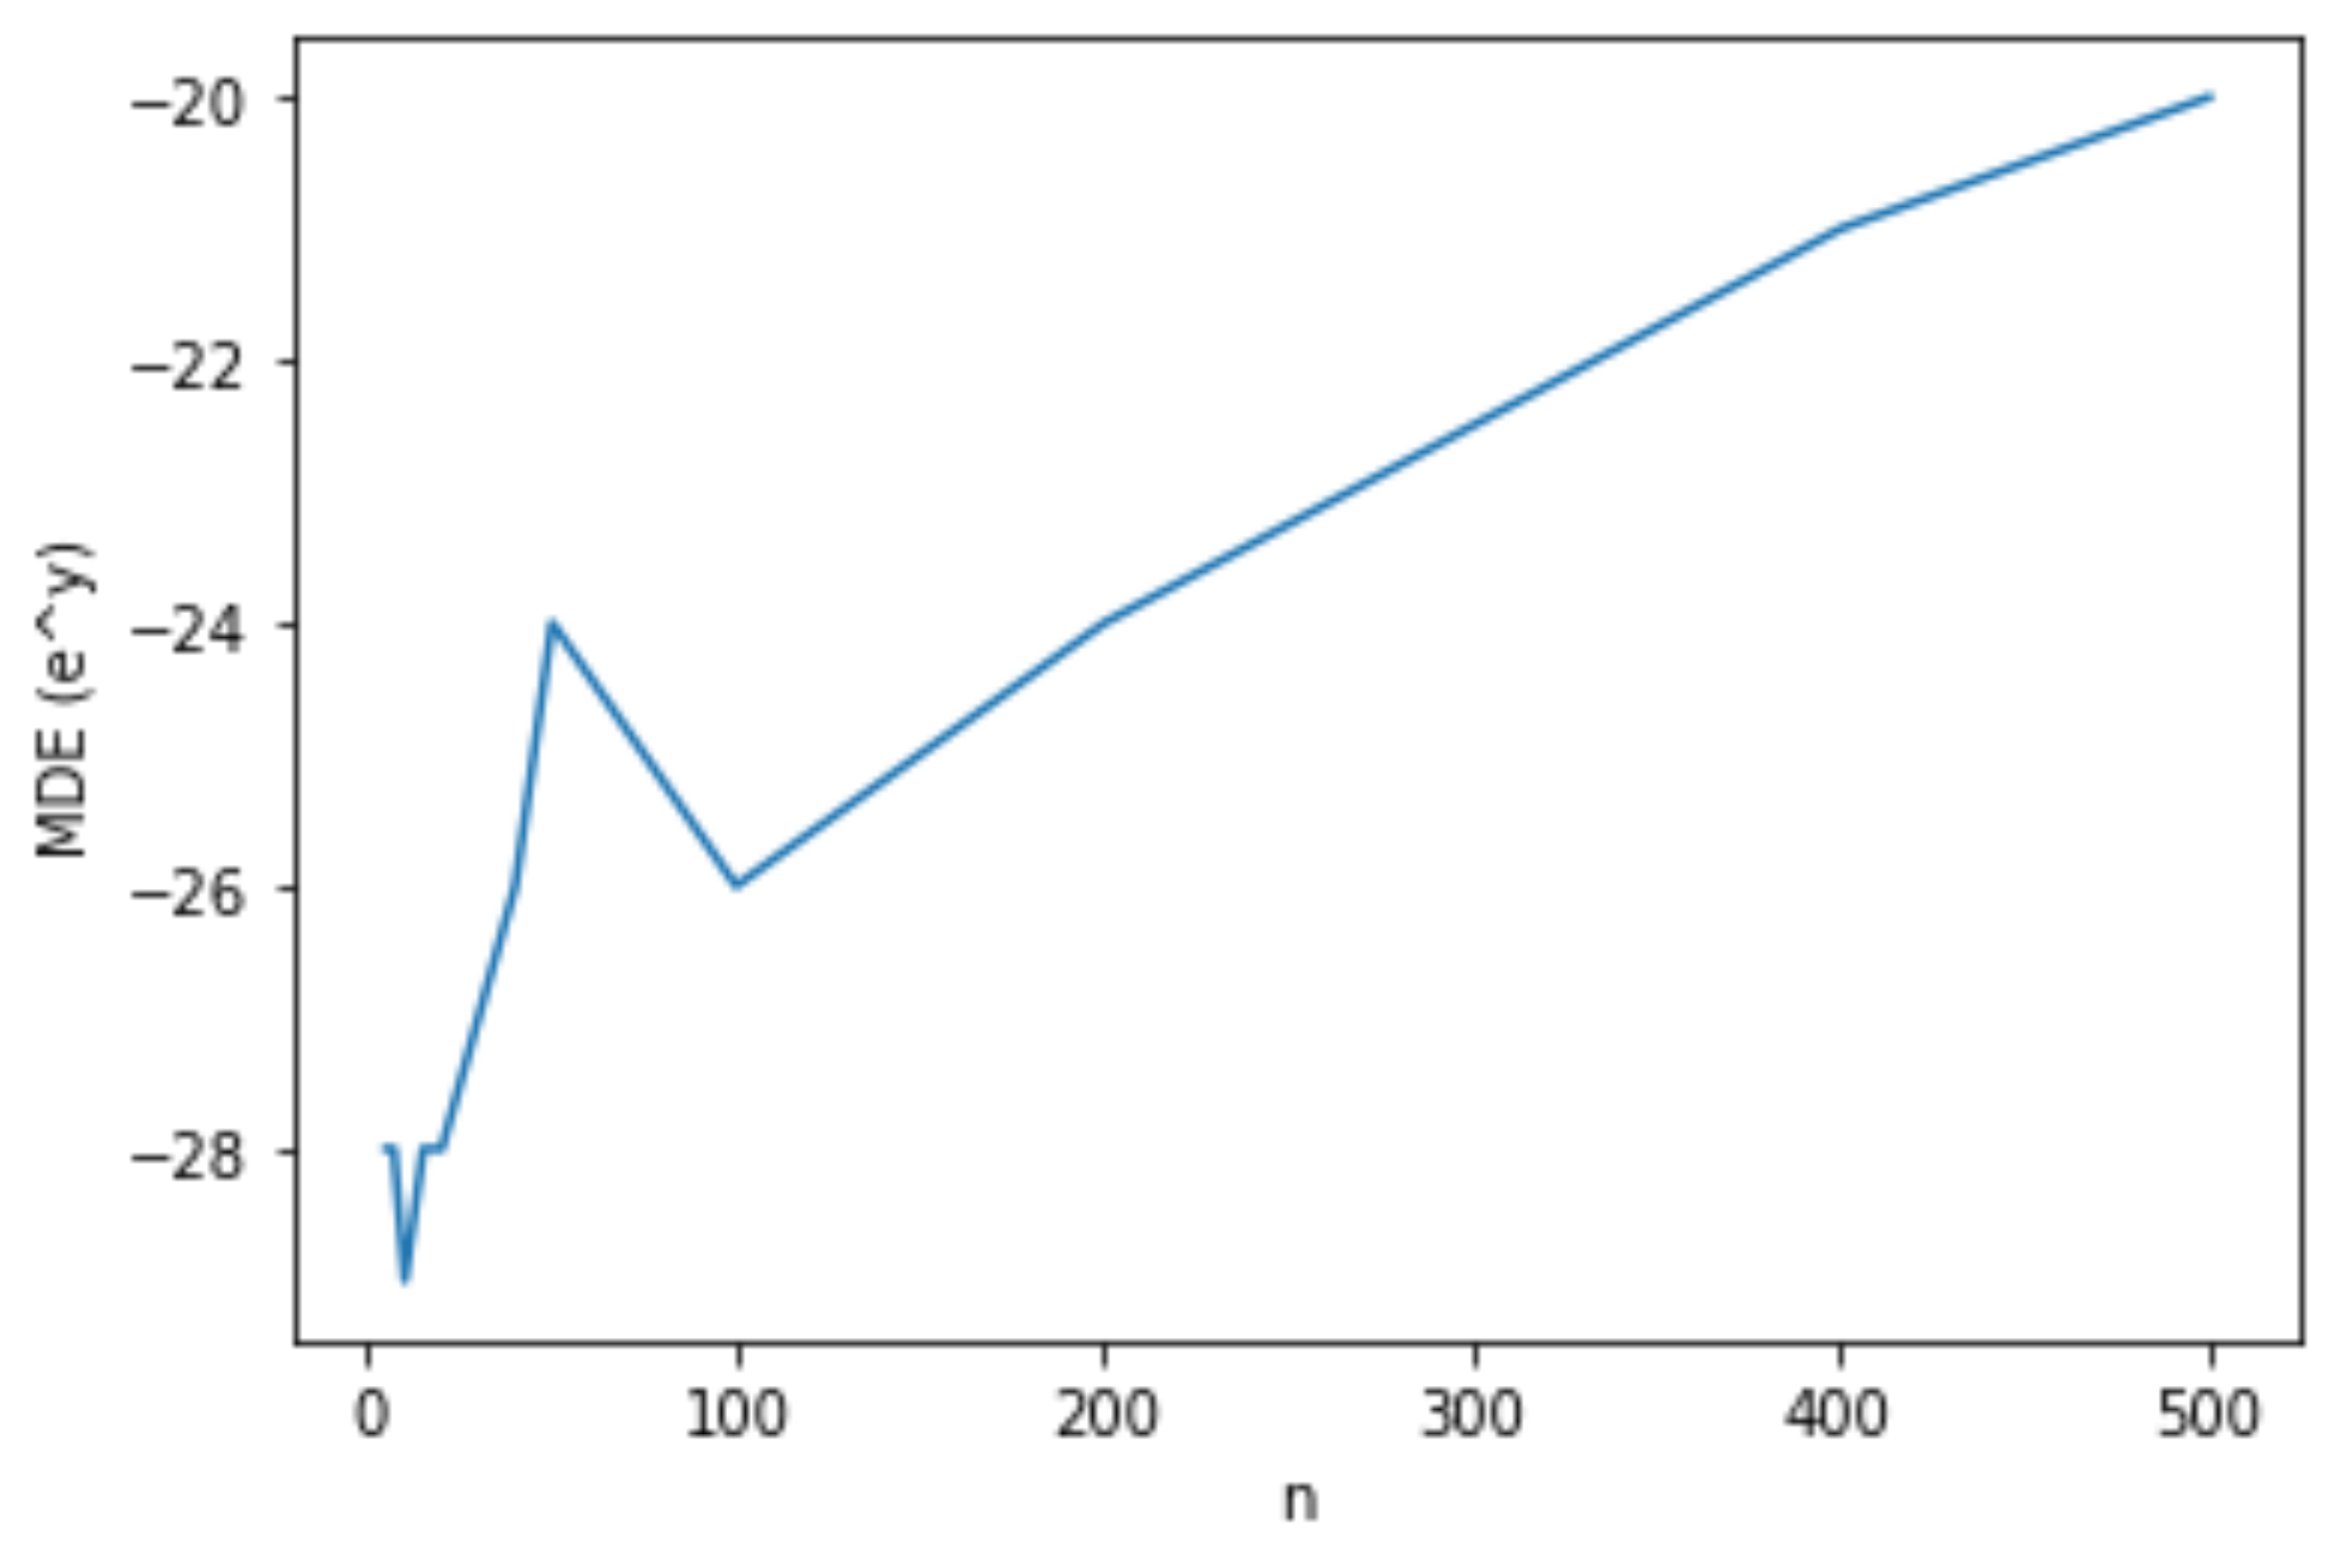
\includegraphics[width=1\linewidth]{figures/mdeTriPro.png}
					\end{center}
					\label{fig:mdeTri}
				\end{figure}
			\end{minipage}
		\end{center}
		\caption{A esquerda, o tempo de processo e, a direita, a ordem de grandeza associada ao MDE das soluções.}
		\label{fig:triPri}
	\end{figure}
	
	Também simulou-se o Algorítimo~\ref{alg:realizacaoTrilateration}, que teve um comportamento muito similar ao Algorítimo~\ref{alg:realizacaoIterativa}, como era de se esperar. Também usou-se instâncias $n$ variando em $\{5, 6, 7,10,15,20,30,40,50,100,200,400,500\}$. Porém, agora, com uma busca inteligente por vértices adjacentes, pode-se variar $\mathcal{P}$ afim de analisar diferentes geometrias para o problema, como apresenta-se a seguir.
	
	\subsubsection*{Instâncias com 70\% de arestas}
	
	\begin{figure}[H]
		\begin{center}
			\begin{minipage}{0.45 \linewidth}
				\begin{figure}[H]
					\begin{center}
						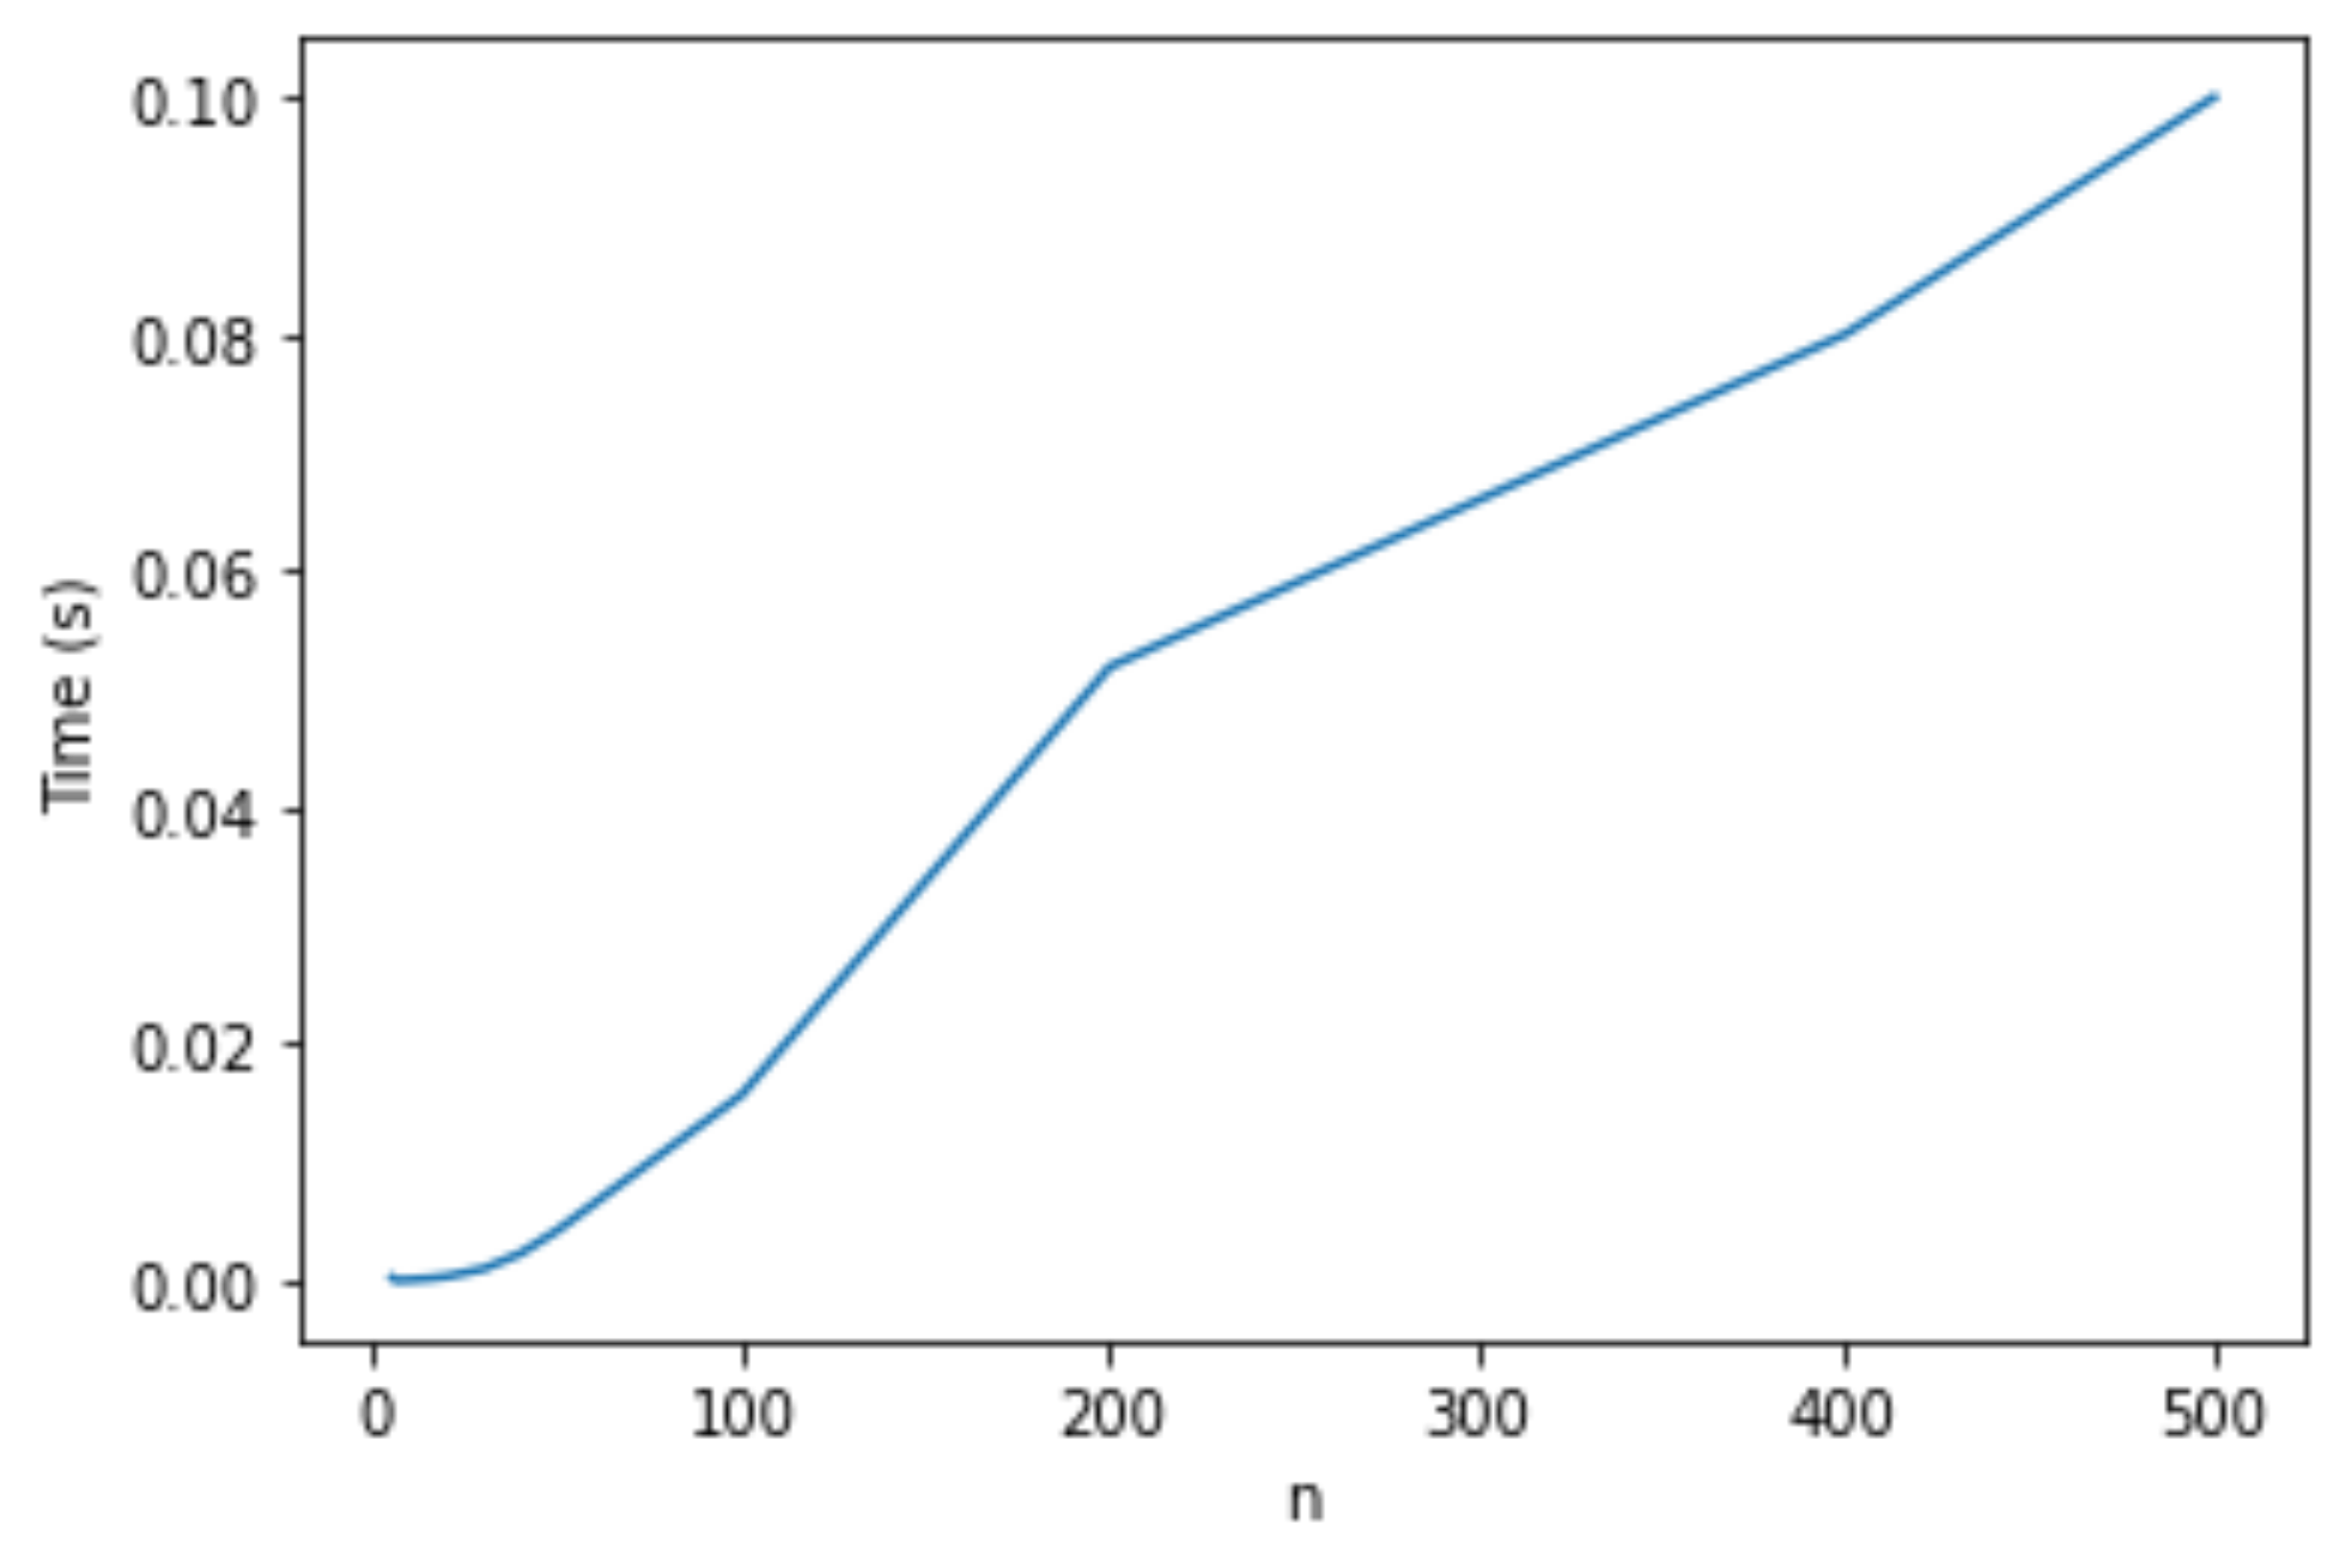
\includegraphics[width=1\linewidth]{figures/timeTriPro1.png}
					\end{center}
				\end{figure}
			\end{minipage}
			\hspace{0.1cm}
			\begin{minipage}{0.45 \linewidth}
				
				\begin{figure}[H]
					\begin{center}
						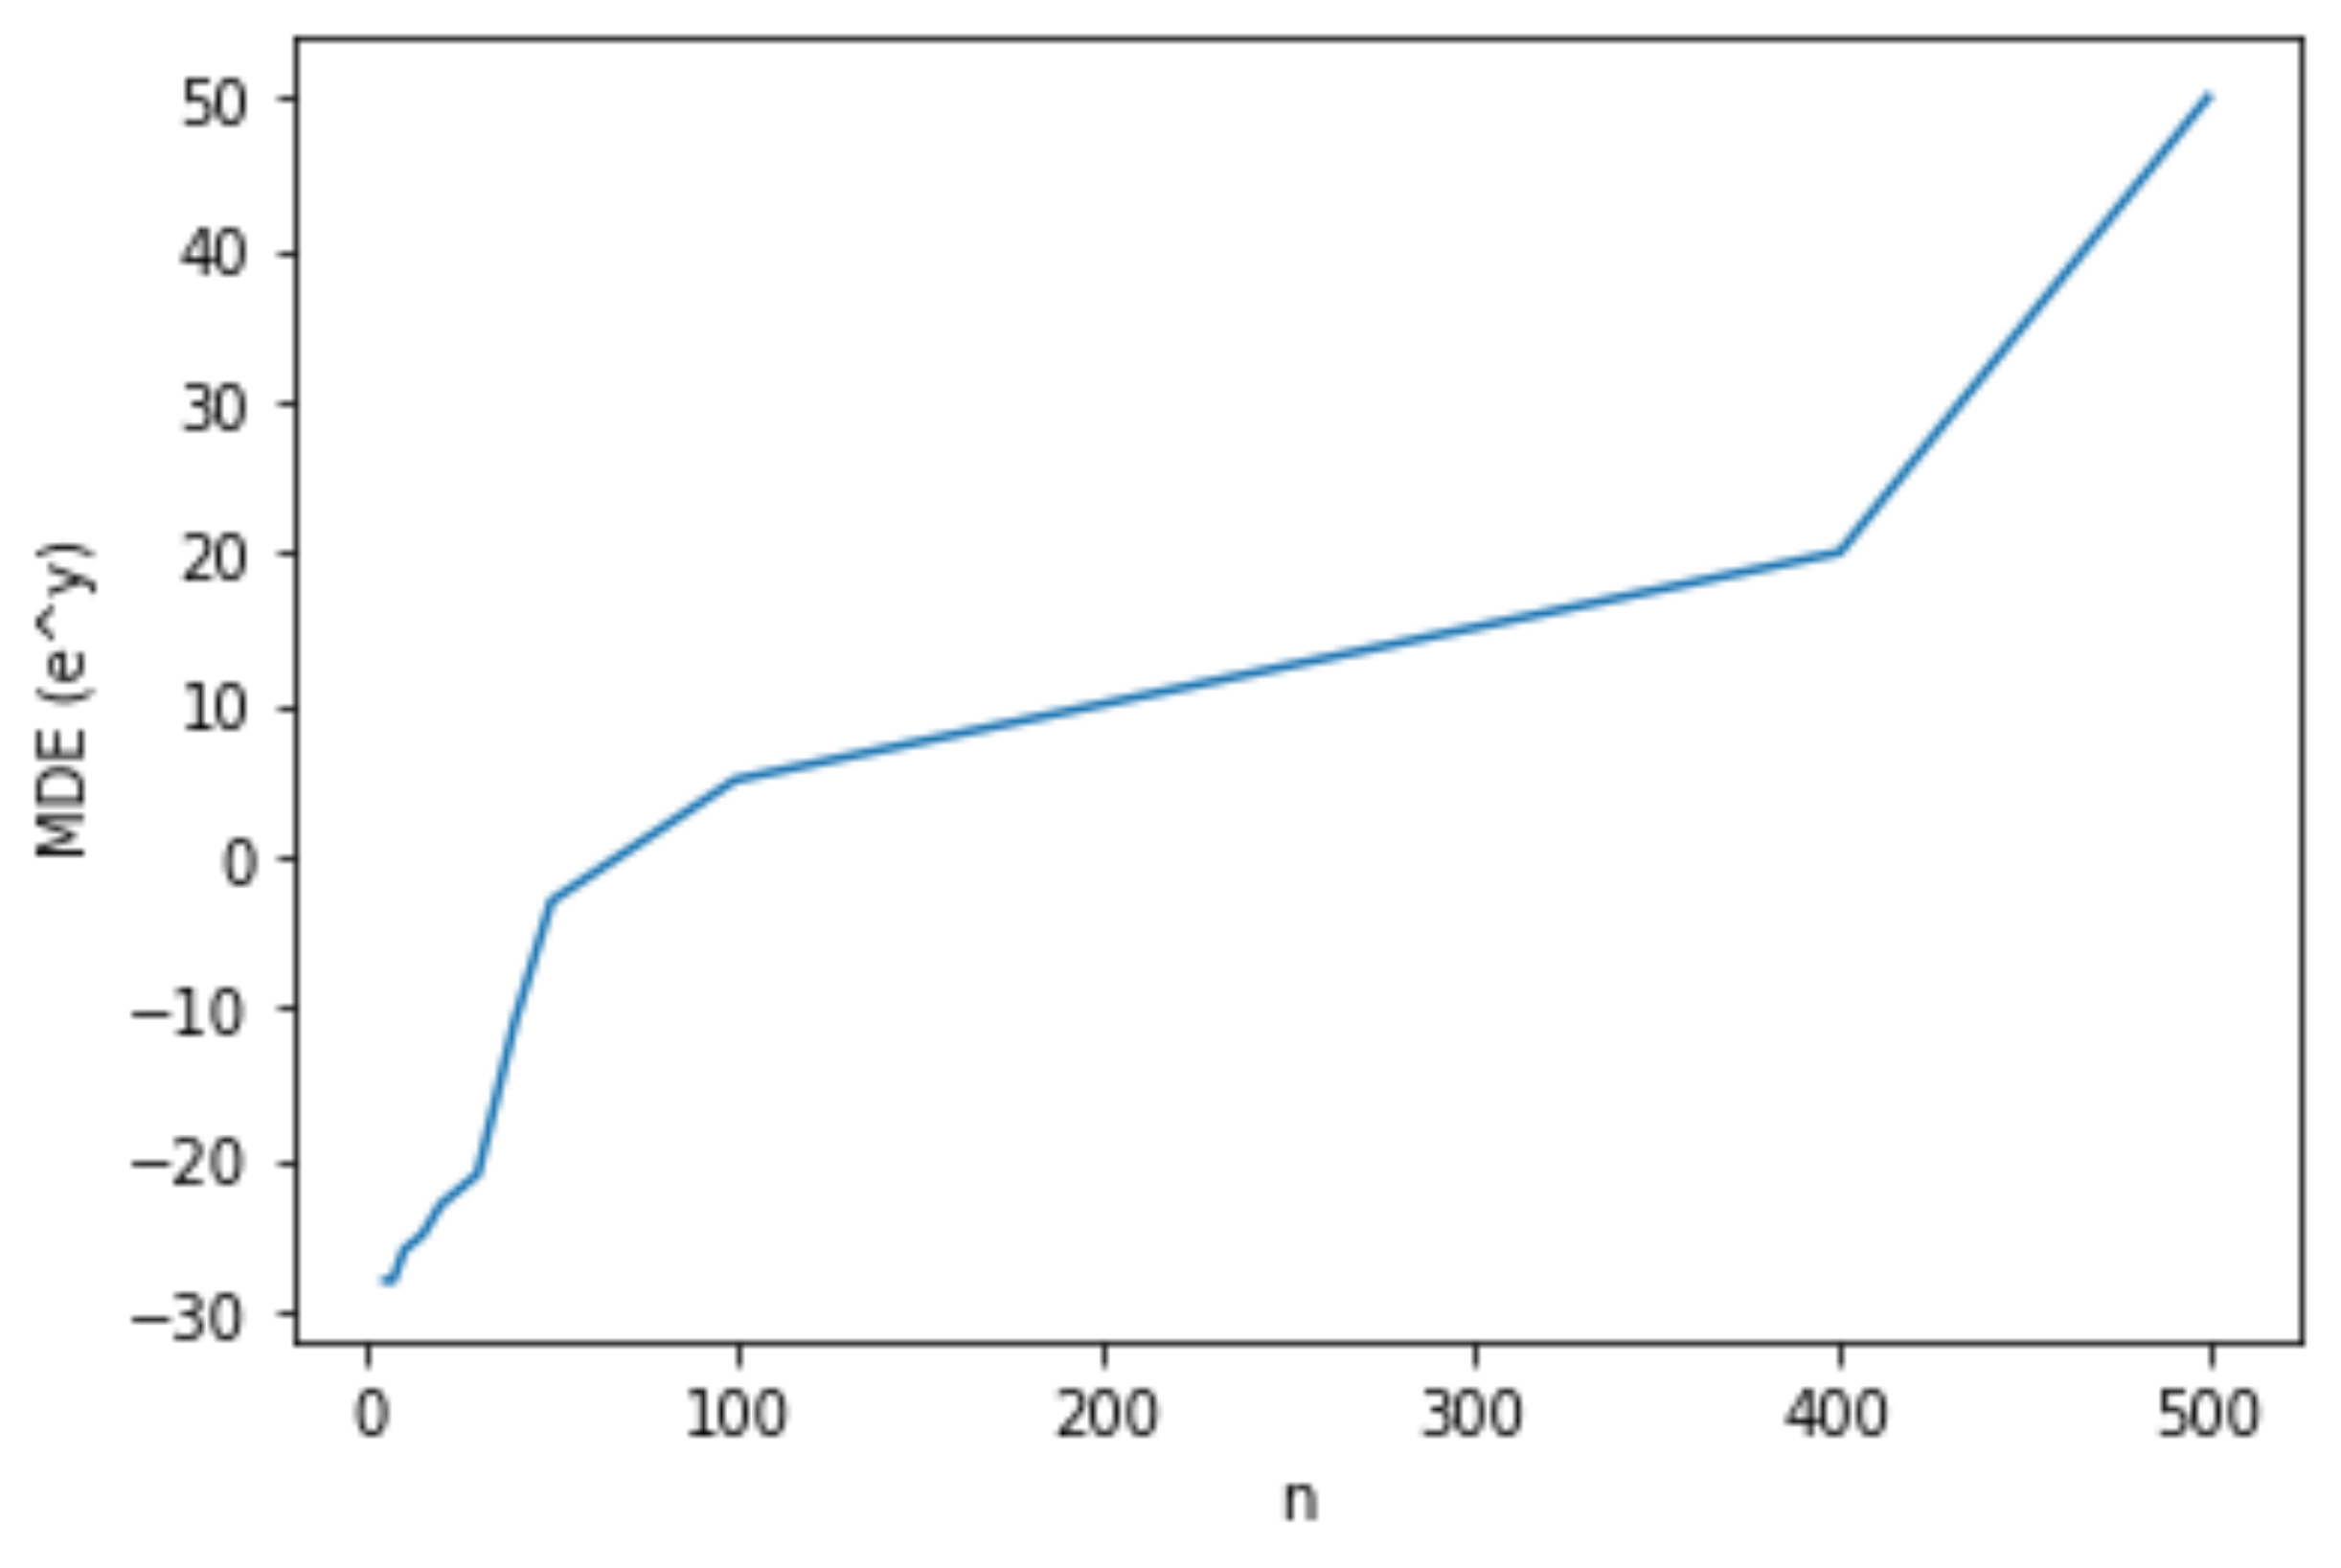
\includegraphics[width=1\linewidth]{figures/mdeTriPro1.png}
					\end{center}
					\label{fig:mdeTri}
				\end{figure}
			\end{minipage}
		\end{center}
		\caption{A esquerda, o tempo de processo e, a direita, a ordem de grandeza associada ao MDE das soluções. Utilizou-se $\mathcal{P} = 0.7$.}
		\label{fig:triPri4}
	\end{figure}
	
	\subsubsection*{Instâncias com 5\% de arestas}
	
	\begin{figure}[H]
		\begin{center}
			\begin{minipage}{0.45 \linewidth}
				\begin{figure}[H]
					\begin{center}
						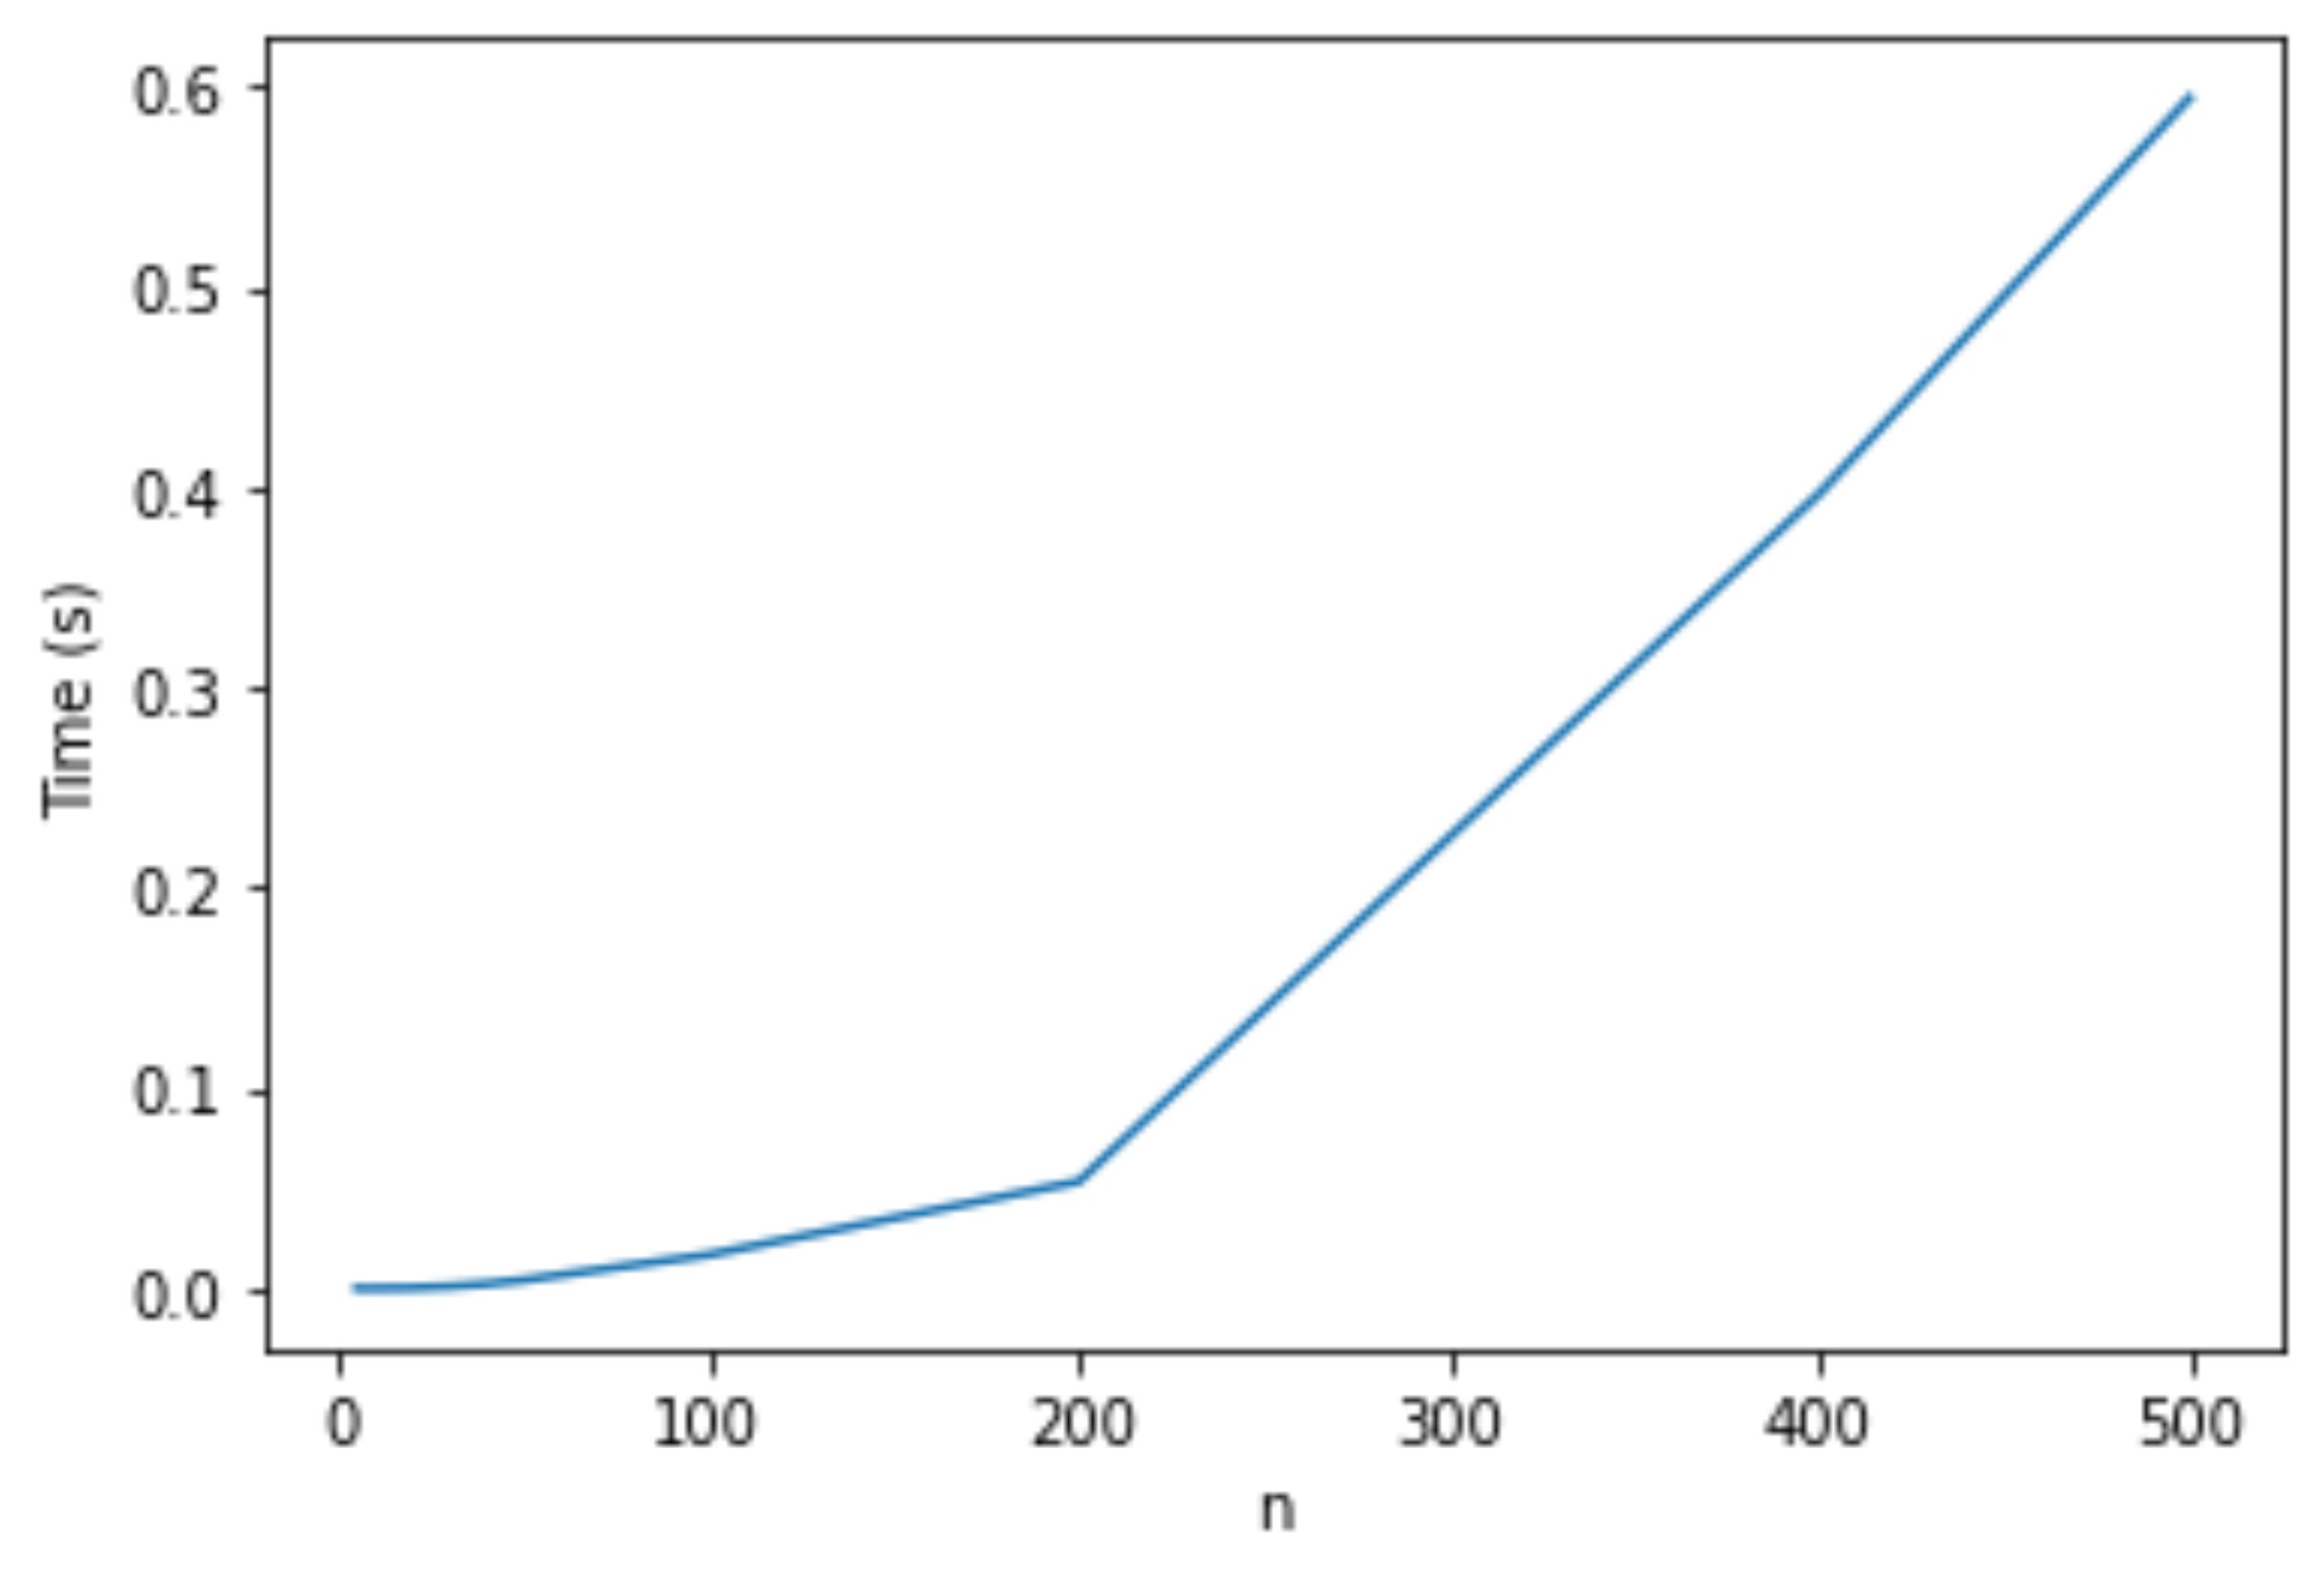
\includegraphics[width=1\linewidth]{figures/timePro2.png}
					\end{center}
				\end{figure}
			\end{minipage}
			\hspace{0.1cm}
			\begin{minipage}{0.45 \linewidth}
				
				\begin{figure}[H]
					\begin{center}
						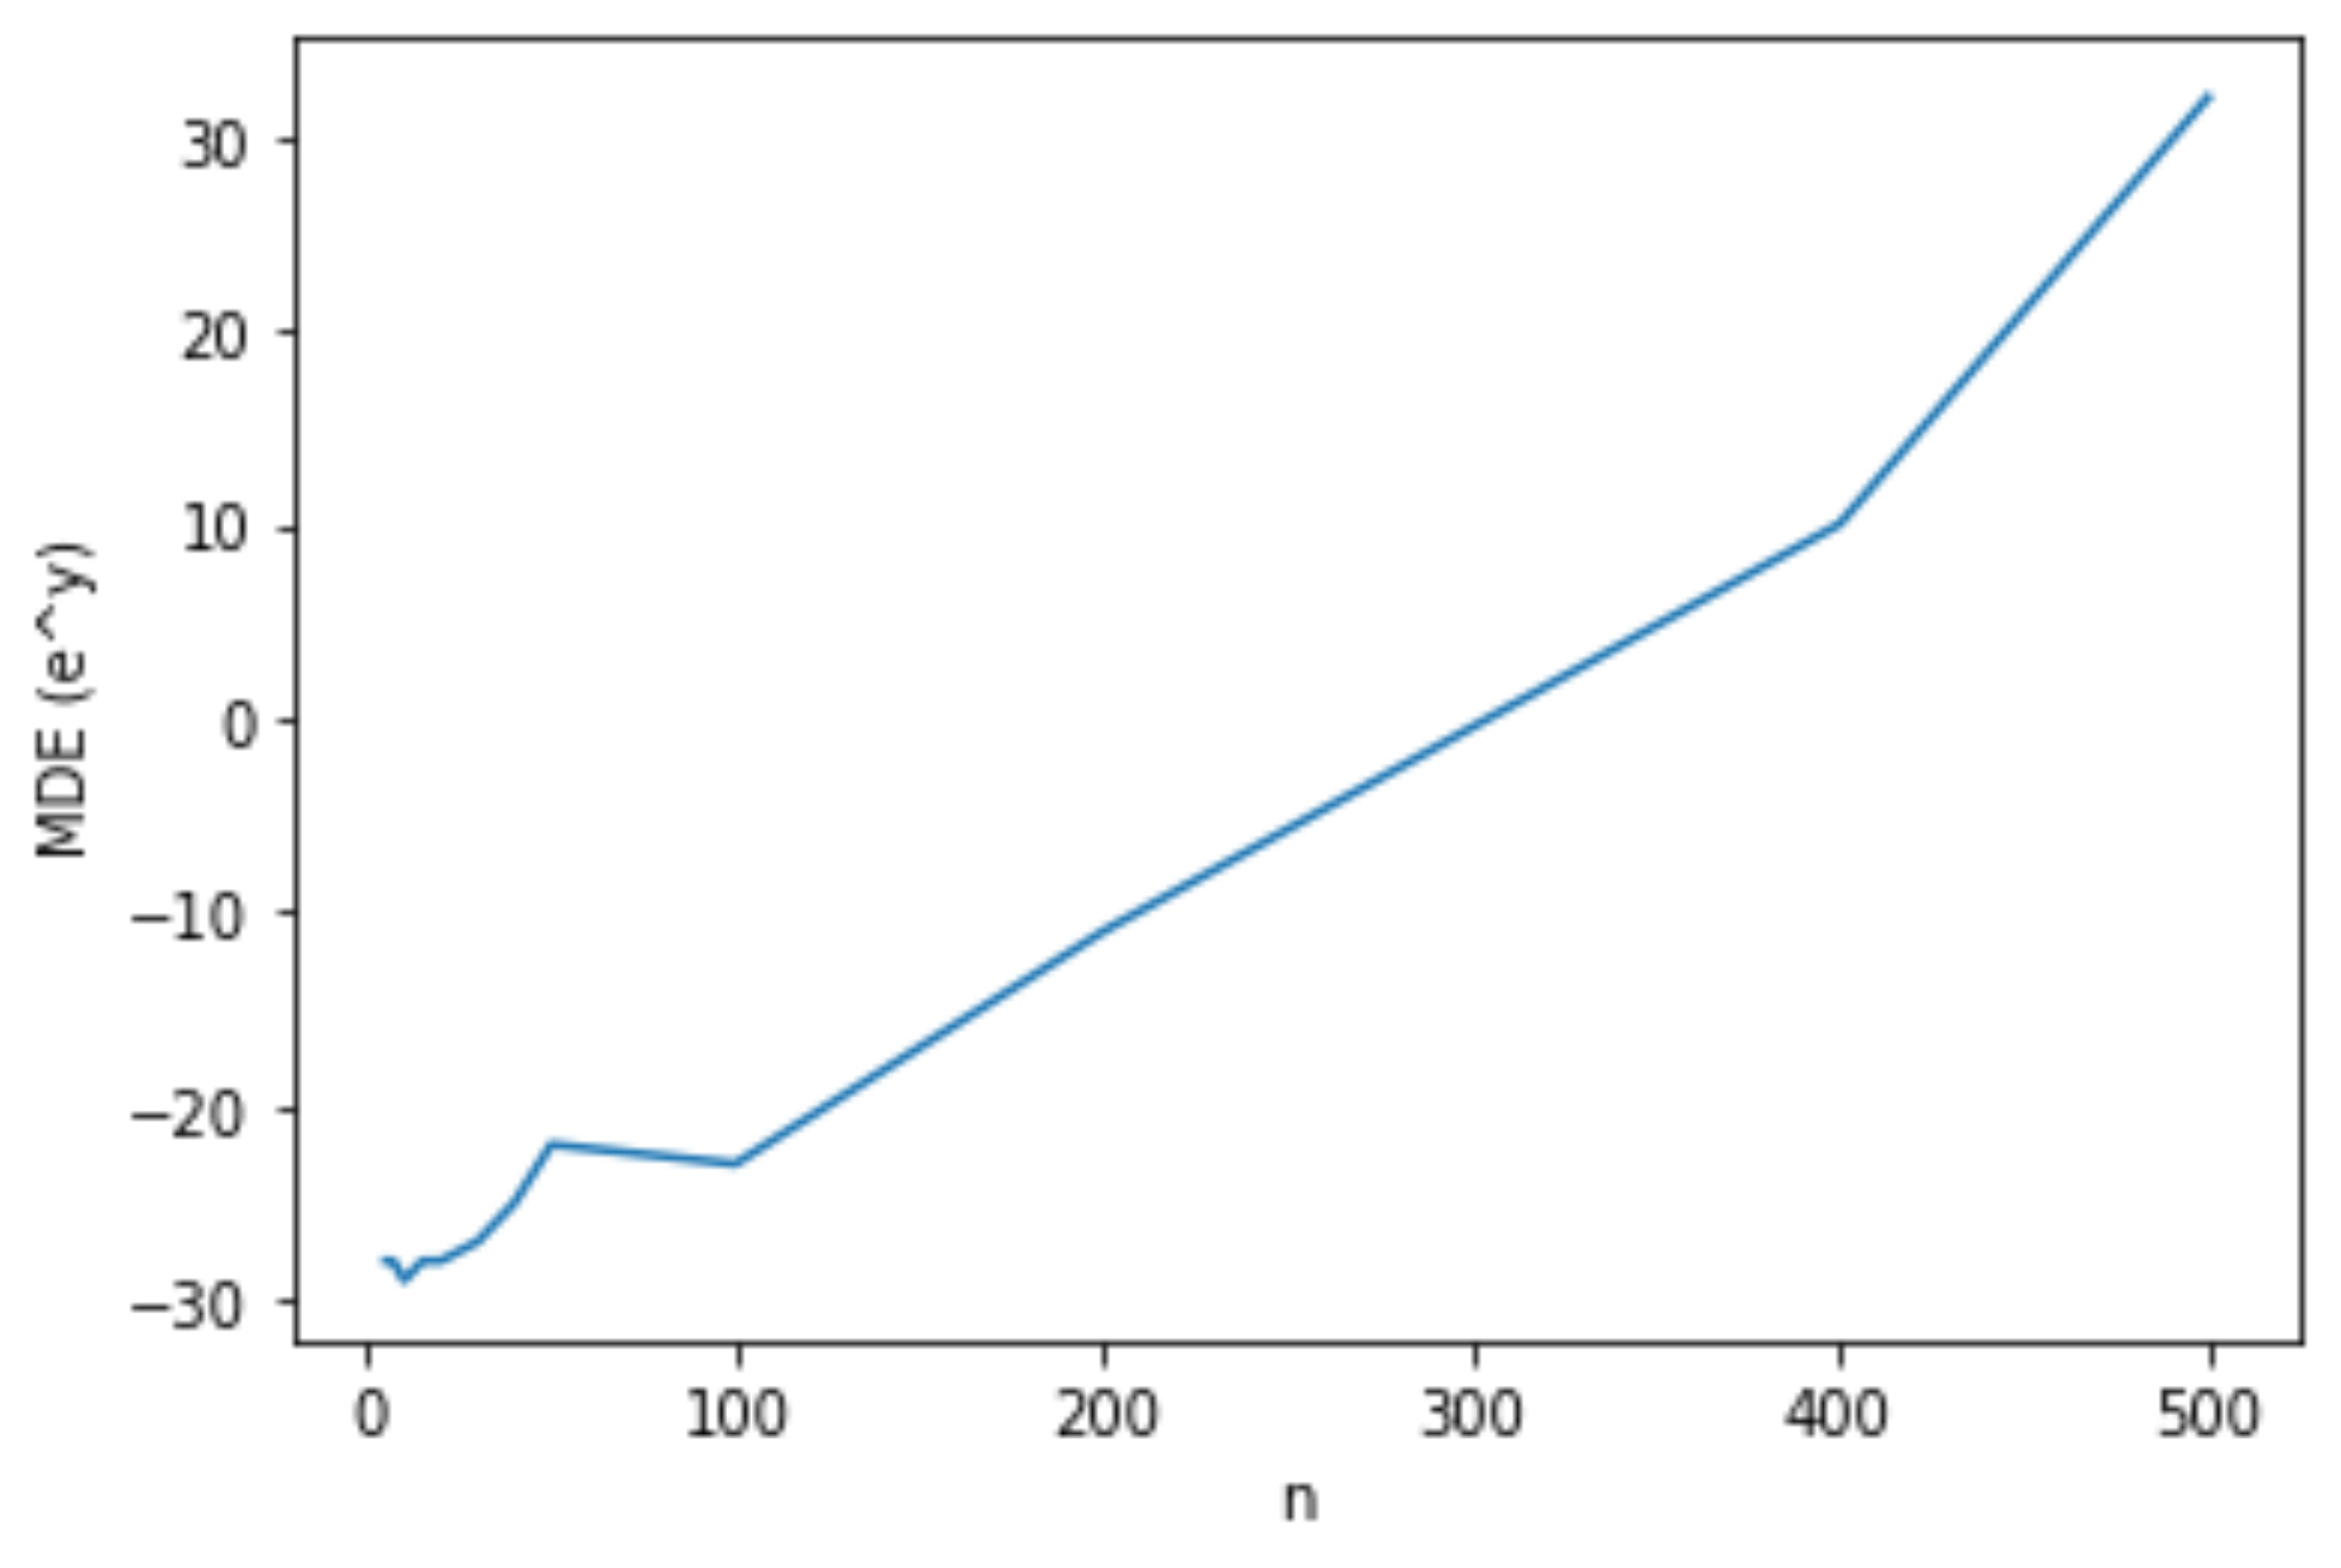
\includegraphics[width=1\linewidth]{figures/mdeTriPro2.png}
					\end{center}
					\label{fig:mdeTri}
				\end{figure}
			\end{minipage}
		\end{center}
		\caption{A esquerda, o tempo de processo e, a direita, a ordem de grandeza associada ao MDE das soluções. Utilizou-se $\mathcal{P} = 0.05$.}
		\label{fig:triPri3}
	\end{figure}
	
	Como esperado, é perceptível uma grande melhora na MDE das soluções conforme se diminui o valor de $\mathcal{P}$. 
	
	Também deve-se perceber que o tempo não obedeceu um padrão perfeito. Podemos relacionar esse fato com a aleatoriedade das instâncias, como pode-se notar que o Algoritmo~\ref{alg:realizacaoTrilateration} teve maios volatilidade no padrão temporal. Mesmo assim, há um consenso. As soluções mostradas nas Figuras~\ref{fig:triPri} e~\ref{fig:triPri3}, por exemplo, demonstram claramente um padrão polinomial, indo de encontro com o que foi apresentado na seção~\ref{sec:oi}.
	
	\newpage
	\section{Considerações Finais}
	Com isso, concluí-se o estudo sobre a Geometria de Distâncias aplicada ao problema de localização de sensores, tal qual teve como resultado um algorítimo que garante encontrar a solução do problema (se houver). .
	\\
	
	Nos cabe, nesse momento, voltarmos atenção às propostas levantadas internamente no início do projeto e verificar se elas foram cumpridas. Seguem o conjunto de objetivos específicos desse projeto, munidos de breve conclusão:
	
	\begin{enumerate}
		
		\item Estudar formas viáveis (pelos vieses energético, de construção e precisão da medida) para obtenção das distâncias entre os elementos do sistema físico:
		
		Fortemente embasado em \cite{savvides2001dynamic} e \cite{sensorsForMobileRobots}, faz-se uma apresentação sobre esses conceitos na Seção~\ref{sec:sensores}. 
		
		\item Estudar as possíveis distribuições dos Robôs Móveis em um sistema genérico, visando verificar quais conjuntos de dados possam ser garantidos como entradas para a construção do problema:
		
		Além de estudar distribuições genéricas, como em \cite{eren2004rigidity}, desenvolve-se na Seção~\ref{sec:disc} o Algorítimo~\ref{alg:instancia}, que cria instâncias aleatórias com diferentes densidades de ligações.
		
		\item Verificar a solução do Discretizable Order Problem \cite{carlileGDandAplications} aplicado ao problema proposto e estudar o ordenamento de vértices que se adeque aos objetivos do trabalho:
		
		Durante o desenvolvimento da Seção~\ref{sec:GD}, percebeu-se que uma ordem de discretização não seria necessária, visto que a definição do problema necessita de uma única solução \cite{libertiEDG}. Por conta disso, definiu-se a ordem de $K$-lateração, que garante a unicidade de solução.
		
		\item Caso consiga-se uma boa ordenação para os vértices, verificar a aplicação do algorítimo Branch-And-Prune \cite{carlile:BP} para a solução do problema proposto. Se não for possível, estudar outros algorítimos que possam solucionar o problema:
		
		Visto que o problema não era discreto, não fora possível aplicar o algorítimo Branch-And-Prune. Ao invés disso, se propôs o Algorítimo~\ref{alg:realizacaoTrilateration}, que utiliza a trilateração como núcleo e garante no máximo uma solução.
		
		\item Estudar a complexidade computacional do algorítimo proposto aplicado as possíveis distribuições:
		
		Isso foi feito no fim das Seções~\ref{sec:GD} e~\ref{sec:disc}, onde verificou-se que o algorítimo pode ser resolvido em tempo polinomial. Também mostrou-se um estudo sobre diferentes visões da geometria do problema afim de minimizar os erros associados. 
		
		\item Simular computacionalmente o algoritmo para solução do problema com instâncias artificialmente geradas, dominando cada passo utilizado:
		
		Simulações apresentadas, de forma satisfatória, na Seção~\ref{sec:disc}.
		
		\item Aplicar o algoritmo estudado em estruturas de pequena escala, como instâncias reais do problema:
		
		Não fora possível cumprir este último objetivo. Infelizmente, a manufatura de robôs móveis usando sensores de distância se demonstrou excessivamente custosa \cite{savvides2001dynamic, sensorsForMobileRobots}.
		
		Vale lembrar, porém, que a utilização de instâncias artificiais genéricas se mostrou de grande importância. Pode-se averiguar e discutir sobre diferentes geometrias, mesmo sem a prototipação de fato.
		
	\end{enumerate}
	
	Como experiências futuras, deseja-se estudar mais sobre a obtenção e tratamento de dados de distâncias, visto que esses possuem erros de medida \cite{sensorsForMobileRobots} (não levados em consideração nesse trabalho). Alguns trabalhos relacionados à Geometria de Distâncias aplicada ao caso intervalar são mostrados em \cite{wsnlSemidefinitePrograming}. Há curiosidade em ver como medida MDE se comporta para uma quantidade grande de vértices associados a erros de medida.
	
	Também deseja-se fazer estudos sobre geometrias mínimas para o problema, como feito em \cite{wsnlFewAnchors}. Deseja-se verificar um conjunto de condições que restringem o movimento de um robô móvel afim de garantir que este ainda possa ser localizado.
	
	\newpage
	\phantomsection
	\addcontentsline{toc}{section}{Referências}
	
	\bibliographystyle{unsrt}
	\bibliography{references}
	
	\newpage
	\appendix
	\input{secGD/apendices.tex}

\end{document}


	\newpage
	\section{Resultados e Discussão \label{sec:disc}}
	Afim de ilustrar e averiguar a eficiência do que foi apresentado aqui, realizou-se algumas simulações computacionais implementando os Algorítimos~\ref{alg:realizacaoIterativa} e~\ref{alg:realizacaoTrilateration} em C. 
	\\
	
	Tais simulações foram executadas em um computador pessoal utilizando o sistema operacional Manjaro (uma distribuição Linux baseada em Arch), equipado com um processador Intel Core i5-8600K (6 núcleos operando em 4.1Ghz) e um pente de memória DDR4 2666MHz de 8Gb em \textit{Single-Channel} (operando, por tanto, em 1333Mhz).	
	\\
	
	Para a eficiência dos algorítimos, fez-se uso da biblioteca de código aberto LAPACKE, que é uma interface para o LAPACK (\textit{Linear Algebra Packge}) em C, onde encontra-se algumas implementações muito otimizadas de operações elementares envolvendo Álgebra Linear. Por exemplo, possui funções para solucionar sistemas matriz-vetor $Ax = b$, através da decomposição matricial LU \cite{AlgebraLinearElon}, que pôde ser usada para solucionar o sistema linear~\ref{eq:DGPLinearSystem}, discutido na seção~\ref{sec:trilateration}.
	
	\subsection{Erro acumulado}
	
	Como tanto o algorítimo~\ref{alg:realizacaoIterativa} quanto o~\ref{alg:realizacaoTrilateration} calculam posições em função de realizações previamente calculadas, é inevitável o acumulo de erros entre essas realizações. Mesmo que a solução teórica seja perfeita, na prática os valores não são representados exatamente. Isso se dá pois o computador não trabalha no conjunto dos números reais, ou, pior, para qualquer $i \in\mathbb{R}$, a possibilidade de $i$ não pode ser representado pelo computador tem probabilidade 1. Por isso, gera-se a necessidade de analisar o quão perto as soluções calculadas estão das reais.
	
	Neste texto, a principal medida de confiabilidade de uma solução será calculada através da \textit{Mean Distance Error}, como segue \cite{mucherino:BP}.
	
	\begin{center}
		\begin{minipage}{0.9 \linewidth}
			\textbf{\textit{Mean Distance Error} (MDE)}: Seja $G= (V,E,d)$ um grafo ponderado que defina uma instância DGP. Se $\{x_1, \dots, x_n\}$ é um conjunto que define uma realização dos $n$ vértices de $G$ e então,
			$$MDE(x) = \frac{1}{|d\;|} \sum_{i,j}^{}\frac{|||x_i - x_j|| - d_{i,j}|}{d_{i,j}} .$$
		\end{minipage}
	\end{center}
	
	\subsection{Exemplares utilizados}
	Como entrada das simulações, implementou-se o Algorítimo~\ref{alg:instancia}, que gera um grafo $K$-laterativo com $n$ vértices de coordenadas aleatórias $x_i = (x_{i1},\dots,x_{iK})\in \mathbb{R}^K$ e provê um conjunto limitável de arestas. Esse limitação é definida pelo parâmetro $\mathcal{P} \in [0,1]$, como coeficiente de probabilidade de uma aresta ser ou não acessível entre dois vértices aleatório $v_i$ e $v_j$, com $i,j>K+1$ (garantindo que sempre haverá ao menos uma (K+1)-clique adjacente a todo vértice).
	\\
	
	\begin{algorithm}[H]
		\label{alg:instancia}
		\tcp{Percorra todos os vértices}
		\For{$i\in \{0,\dots,n\}$}{
			\tcp{Varie entre cada coordenada de $x_i\in\mathbb{R}^K$}
			\For{$j \in {1,\dots,K}$}{
				\tcc{Atribua um valor aleatório para cada co. A função Aleatorio(\textit{m}) gera valores entre 0 e \textit{m}.}
				$x_{ij} = $Aleatorio$(m)$; 
			}
		}
		\tcp{Para cada vértice, percorra todos os seus antecessores}
		\For{$x_i \in \{x_n, \dots,x_1\}$}{
			\For{$x_j \in \{x_1, \dots,x_{i-1}\}$}{
				\tcp{Gere um número $a \in [0,1]$ aleatório.}
				Seja $a$ = Aleatorio(1);
				
				\tcp{Verifique se $a > \mathcal{P}$ e se $i,j > K$}
				\If{$a > \mathcal{P}$ and $i > K$ and $j>K$}{
					\tcp{Defina uma aresta entre $x_i$ e $x_j$}
					$e_{i,j} = \|x_i - x_j\|$;
				}
			}
		}
		\textbf{return} $G = (\{v_1,\dots,v_n\}, \{\{e_{1,2}\}, \dots,\{e_{j}\}\})$;
		\caption{$G =$ criaInstancia$(n, \mathcal{P})$}
	\end{algorithm}
	\vspace{0.4cm}
	
	Por exemplo, com o Algorítimo~\ref{alg:instancia} gerou-se a instância mostrada ma Figura~\ref{fig:inst}.
	
	\begin{figure}[H]
	\begin{center}
		\begin{minipage}{0.15 \linewidth}
			\begin{table}[H]
				\centering
				\begin{tabular}{ |c c c| } 
					\hline
					\textbf{x} & \textbf{y} & \textbf{z} \\\hline
					(33, & 36, & 27)\\

					(15, & 43, & 35)\\

					(36, & 42, & 49)\\

					(21, & 12, & 27)\\

					(40, & 9, & 13)\\\hline

				\end{tabular}
				\label{tab:re1}
			\end{table}
		\end{minipage}
	\hspace{0.1cm}
		\begin{minipage}{0.8 \linewidth}
			$$
			\begin{bmatrix}
			 0.000000 & 20.904545 & 23.000000 & 26.832816 & 31.208973\\

			20.904545 & 0.000000 & 25.258662 & 32.572995 & 47.592016\\

			23.000000 & 25.258662 & 0.000000 & 40.112342 & 49.000000\\

			26.832816 & 32.572995 & 40.112342 & 0.000000 & 23.790755\\

			31.208973 & 47.592016 & 49.000000 & 23.790755 & 0.000000	
			\end{bmatrix}
			$$
		\end{minipage}
	\end{center}
\caption{A esquerda, as coordenadas dos vértices gerados e, a direita, a matriz de distância a eles associados.}
\label{fig:inst}
\end{figure}
	
	\subsection{Simulações}
	
	Primeiramente. para gerar instâncias do algorítimo~\ref{alg:realizacaoIterativa}, deve-se usar o algorítimo~\ref{alg:instancia} com $\mathcal{P} = 100$. Assim pode-se garantir a geração de um grafo completo. Criou-se, então, instâncias com tamanhos variados: $n \in \{5, 6, 7,10,15,20,30,40,50,100,200,400,500\}$. A seguir apresenta-se alguns gráficos sobre os resultados.
	
	\begin{figure}[H]
		\begin{center}
			\begin{minipage}{0.45 \linewidth}
				\begin{figure}[H]
					\begin{center}
						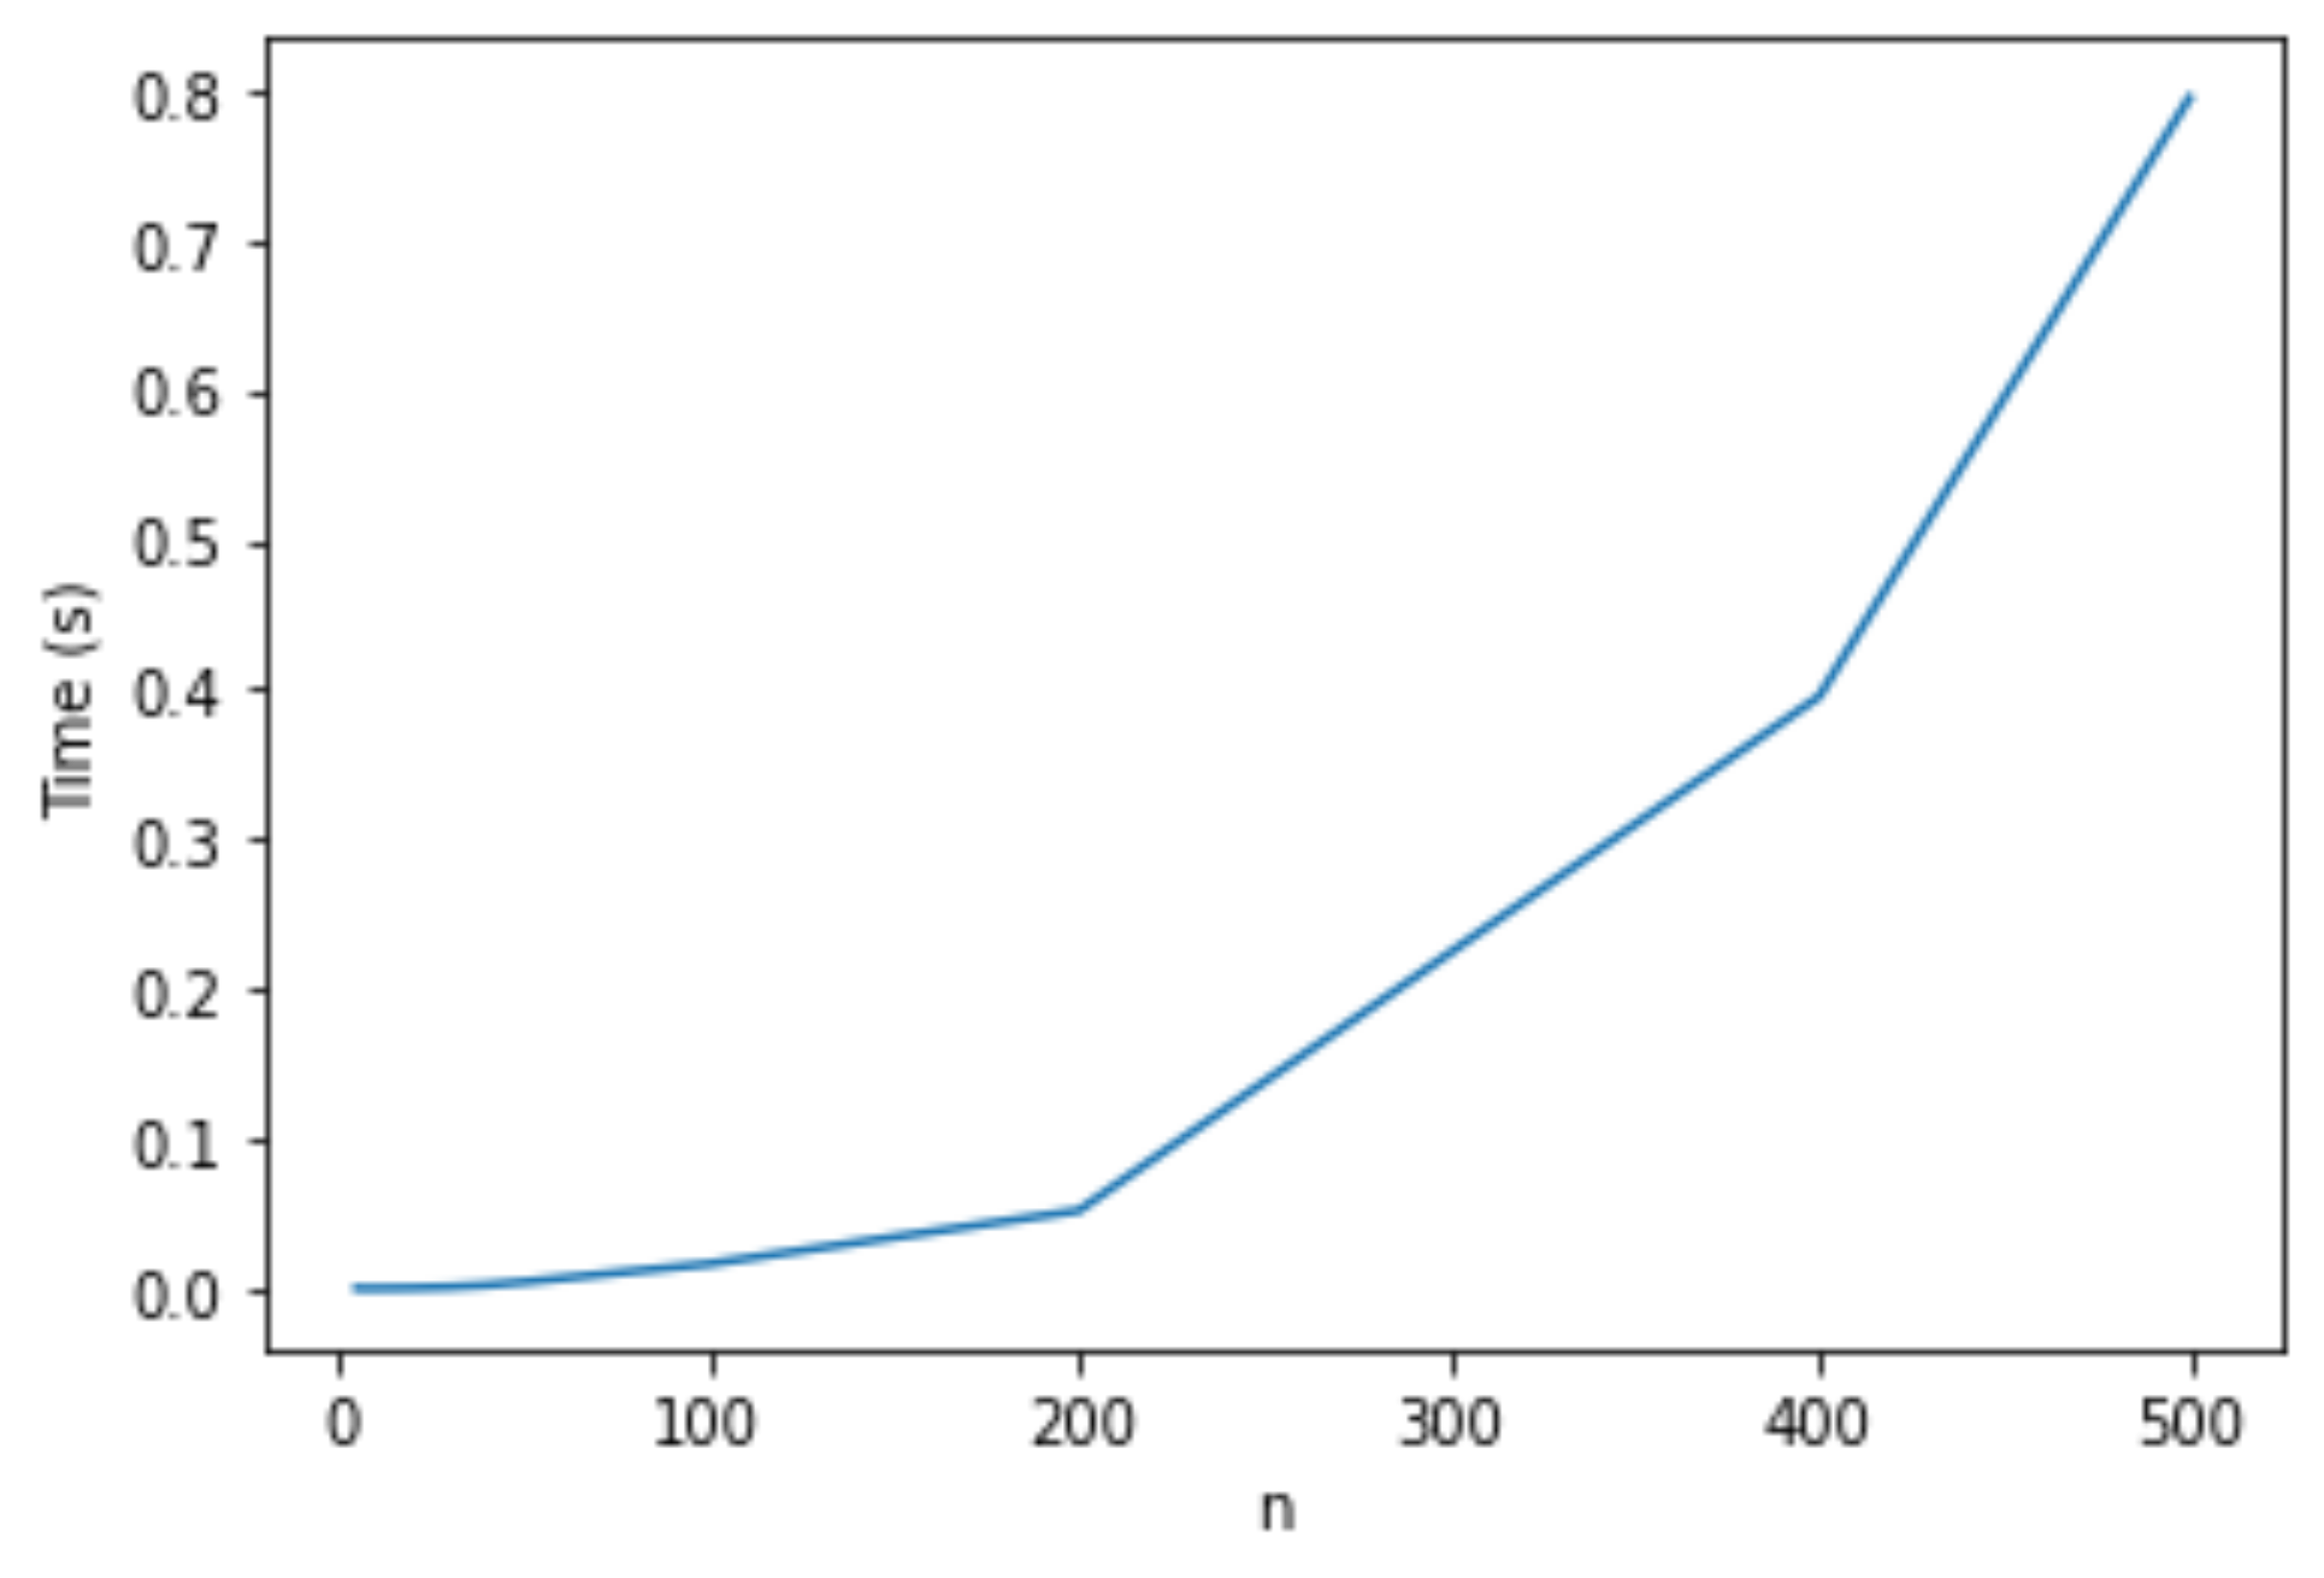
\includegraphics[width=1\linewidth]{figures/tempoTri.png}
					\end{center}
				\end{figure}
			\end{minipage}
			\hspace{0.1cm}
			\begin{minipage}{0.45 \linewidth}
				
				\begin{figure}[H]
					\begin{center}
						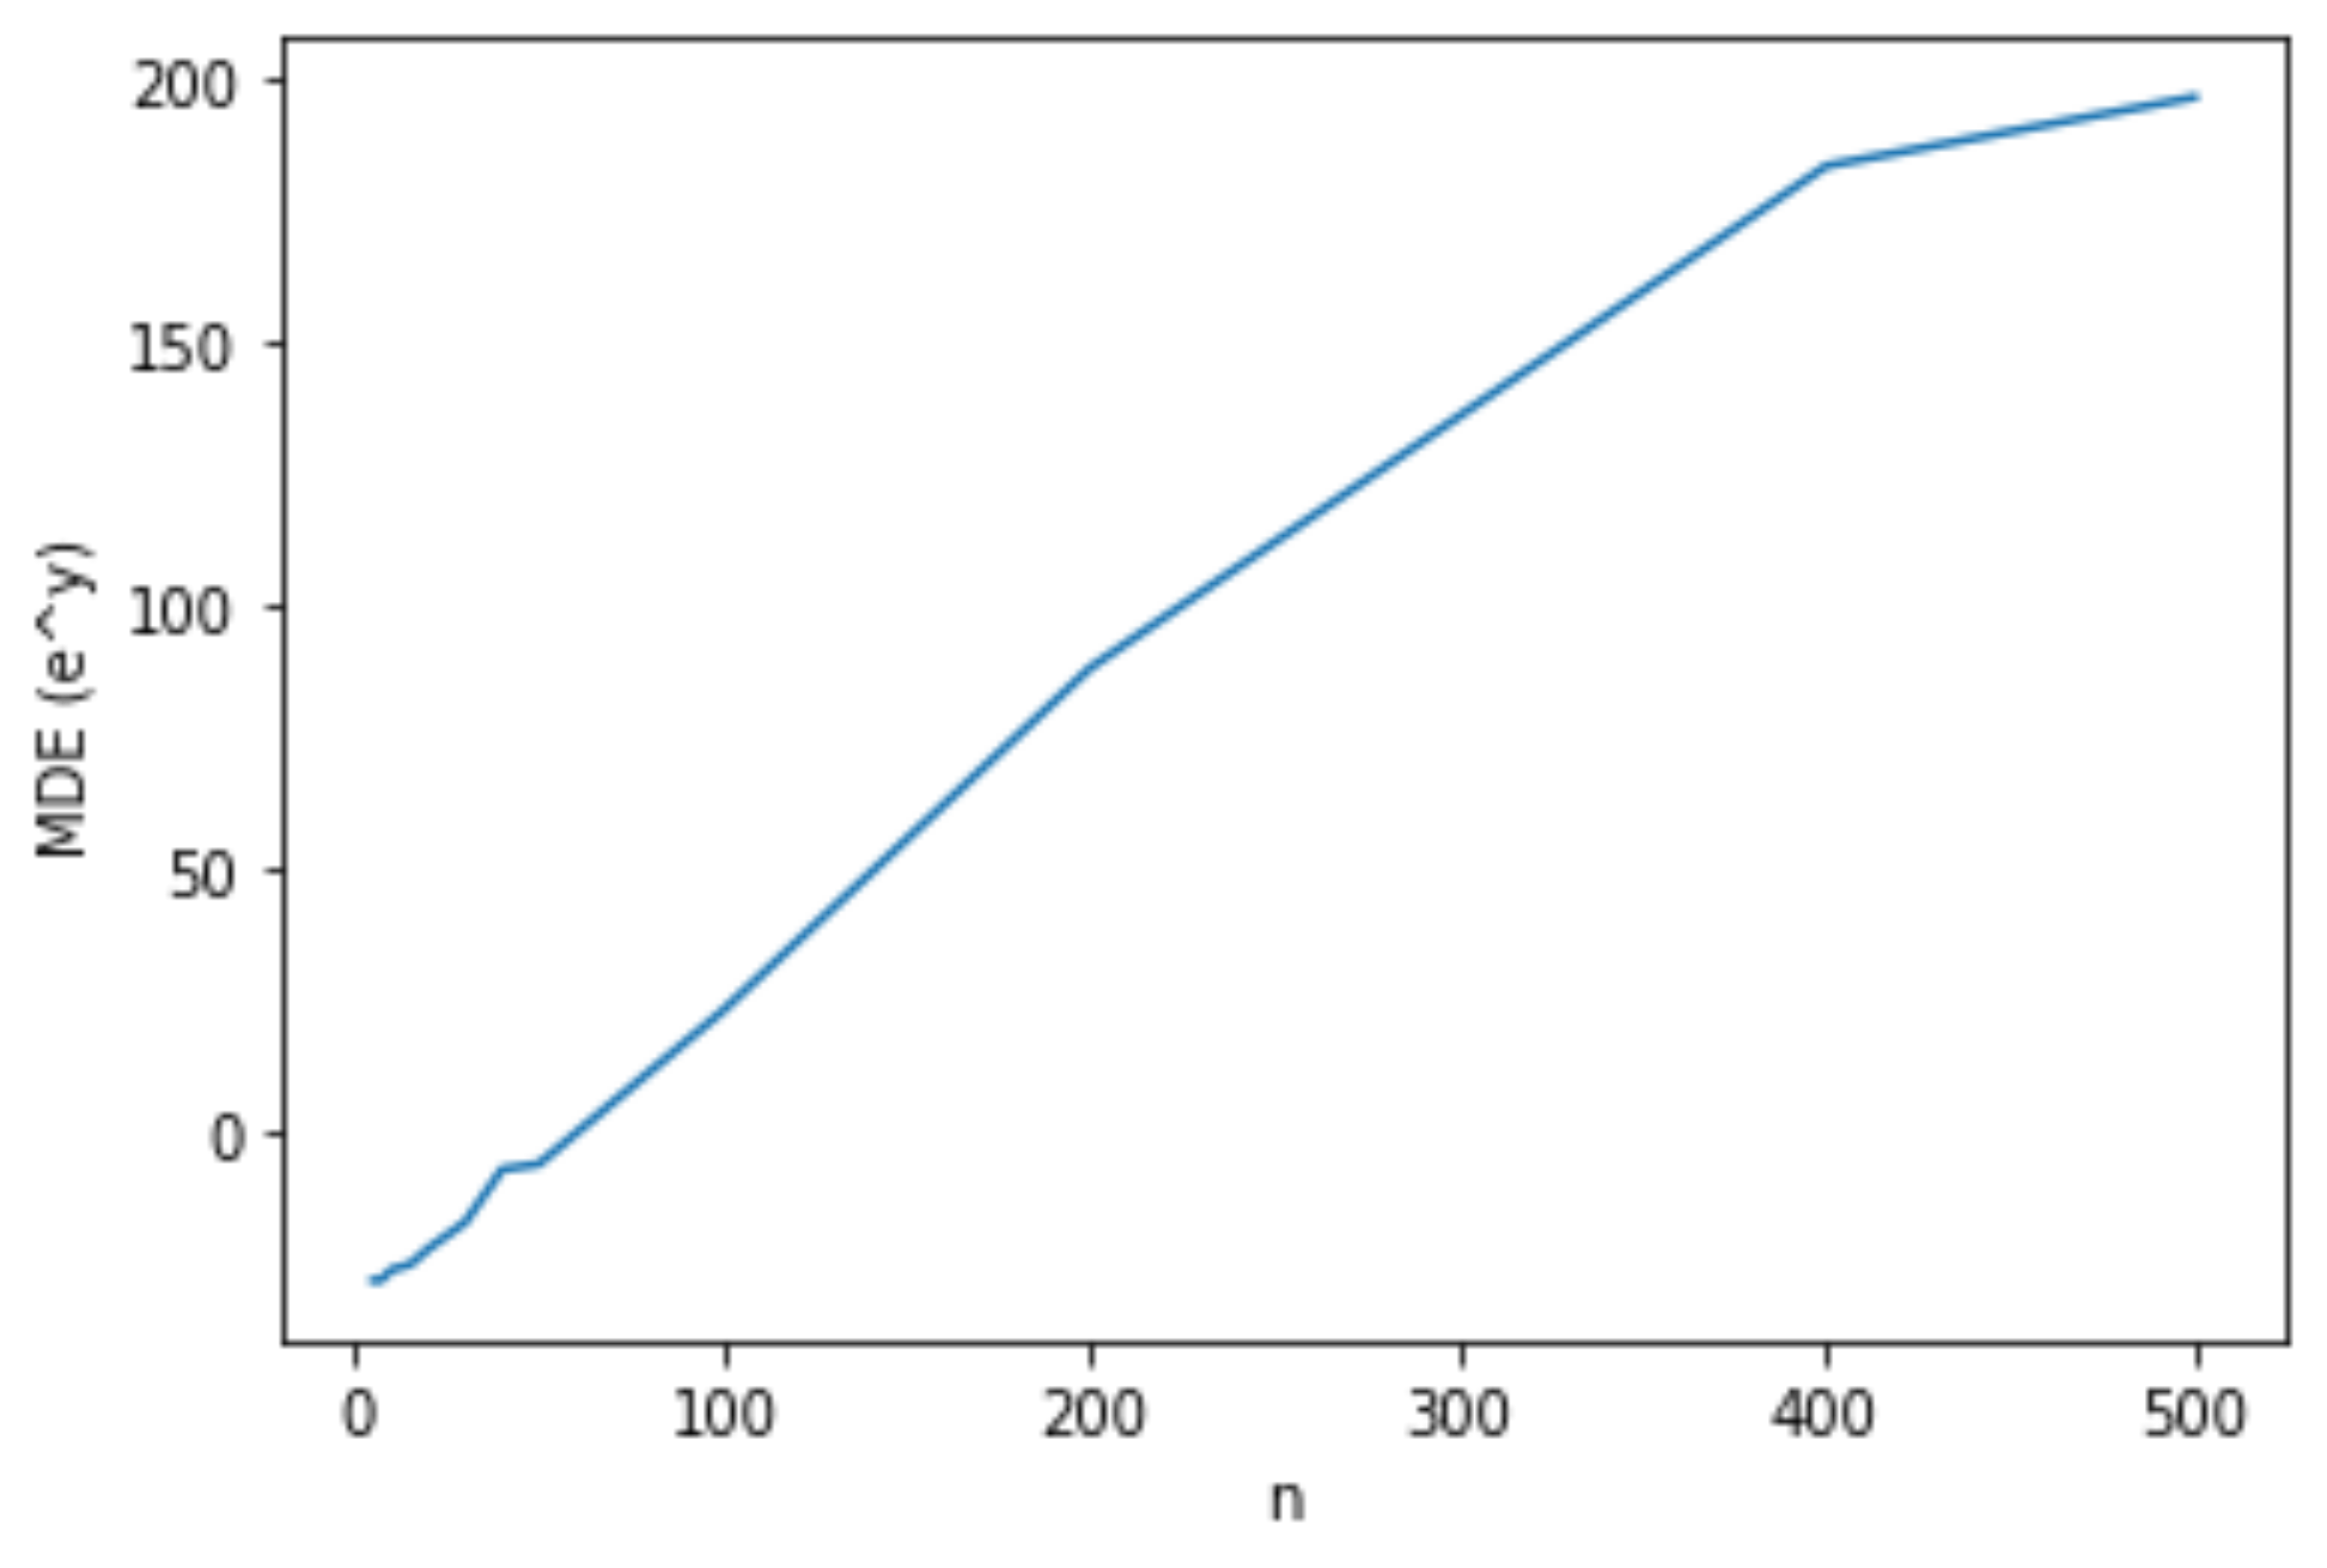
\includegraphics[width=1\linewidth]{figures/mdeTri.png}
					\end{center}
				\end{figure}
			\end{minipage}
		\end{center}
		\caption{A esquerda, o tempo de processo e, a direita, a ordem de grandeza associada ao MDE das soluções.}
		\label{fig:tri}
	\end{figure}
	
	Perceba o comportamento mostrado na Figura~\ref{fig:tri}. Teve-se que fazer uma linearização no gráfico que representa o MDE da solução, pois este cresceu exponencialmente e foi para a ordem de $10^{200}$ em 500 vértices. Esse comportamento se deu por conta dos erros acumulados entre as iterações.
	\\
	
	Uma proposta pensada para contornar essa situação infeliz foi alterar o valor de $\mathcal{P}$, deixando o menor, obrigando o algorítimo a calcular realizações utilizando vértices iniciais. Porém, isso implicaria em um grafo não completo, o que não condiz definição do Algorítimo~\ref{alg:realizacaoIterativa}.
	
	Outra solução proposta fora de utilizar sempre os primeiros vértices no lugar dos antecessores mais próximos. Isso significaria utilizar sempre os vértices âncoras para realizar os demais, semelhante com o que é feito no sistema GPS. Com isso, tivemos os resultados satisfatórios apresentados pela Figura~\ref{fig:triPri}. Perceba que mesmo com 500 vértices ainda obteve-se resultados com $MDE$ na ordem de $10^{-20}$.
	
	\begin{figure}[H]
		\begin{center}
			\begin{minipage}{0.45 \linewidth}
				\begin{figure}[H]
					\begin{center}
						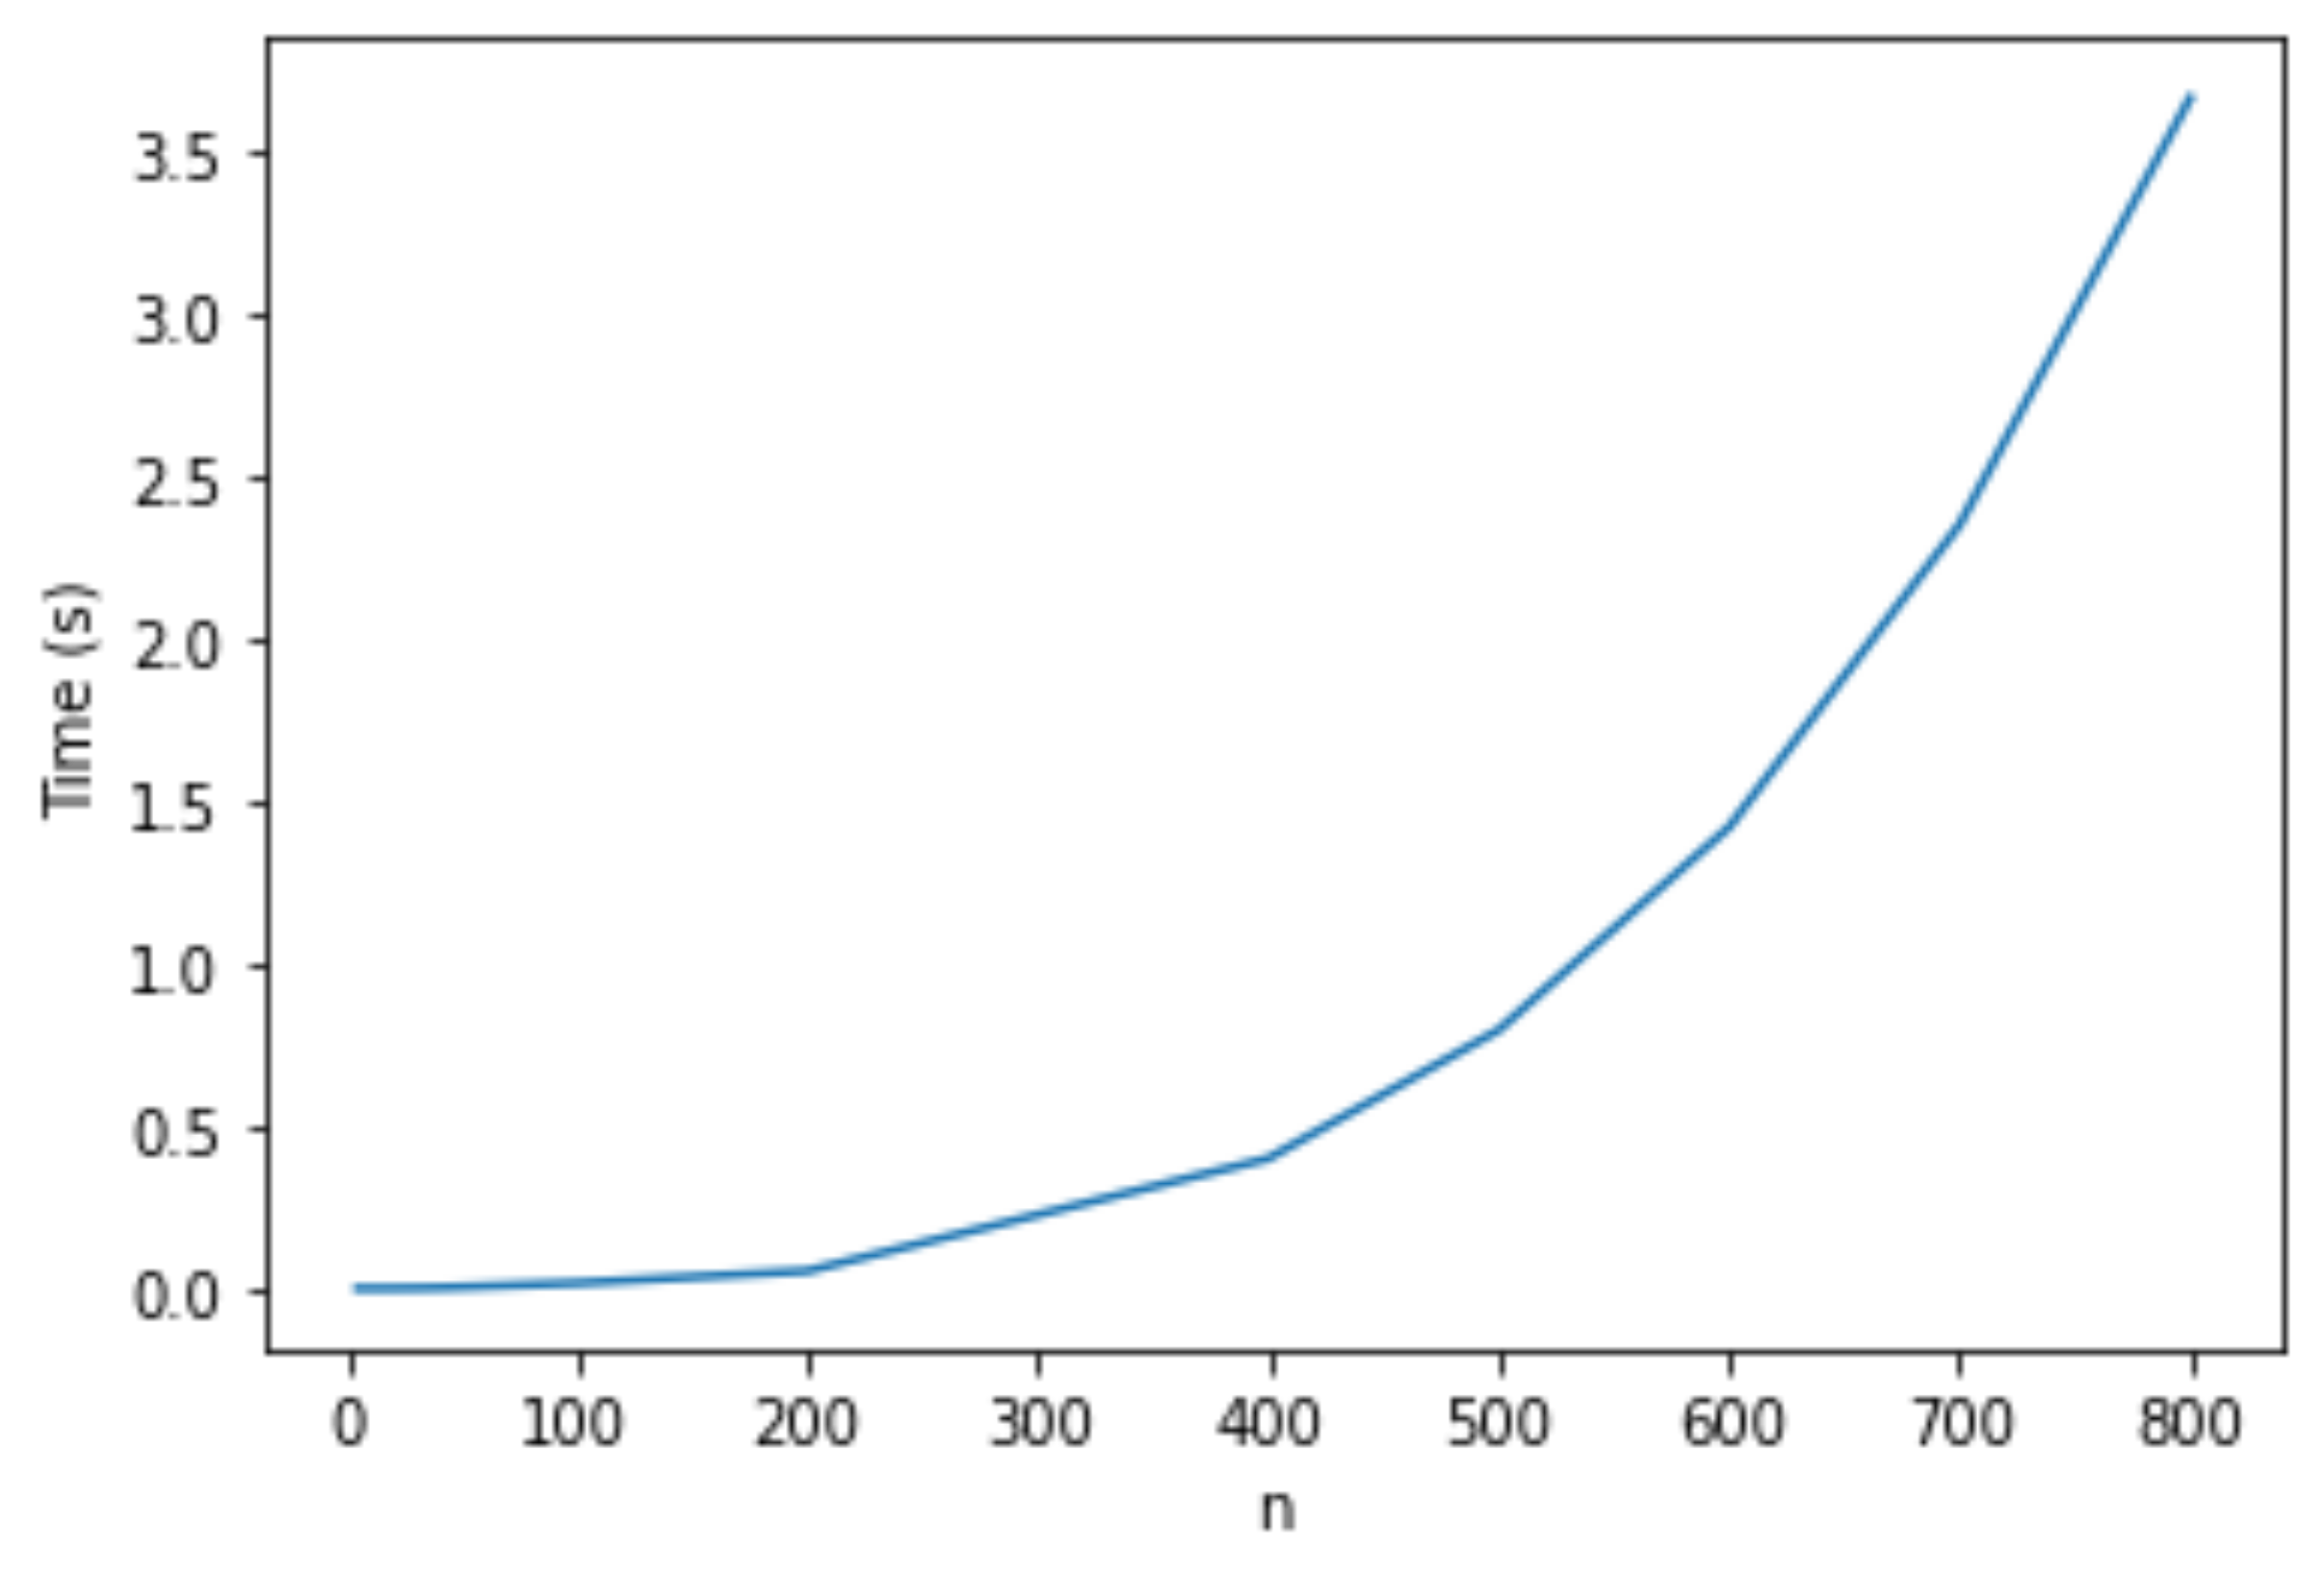
\includegraphics[width=1\linewidth]{figures/tempoTriPri.png}
					\end{center}
				\end{figure}
			\end{minipage}
			\hspace{0.1cm}
			\begin{minipage}{0.45 \linewidth}
				
				\begin{figure}[H]
					\begin{center}
						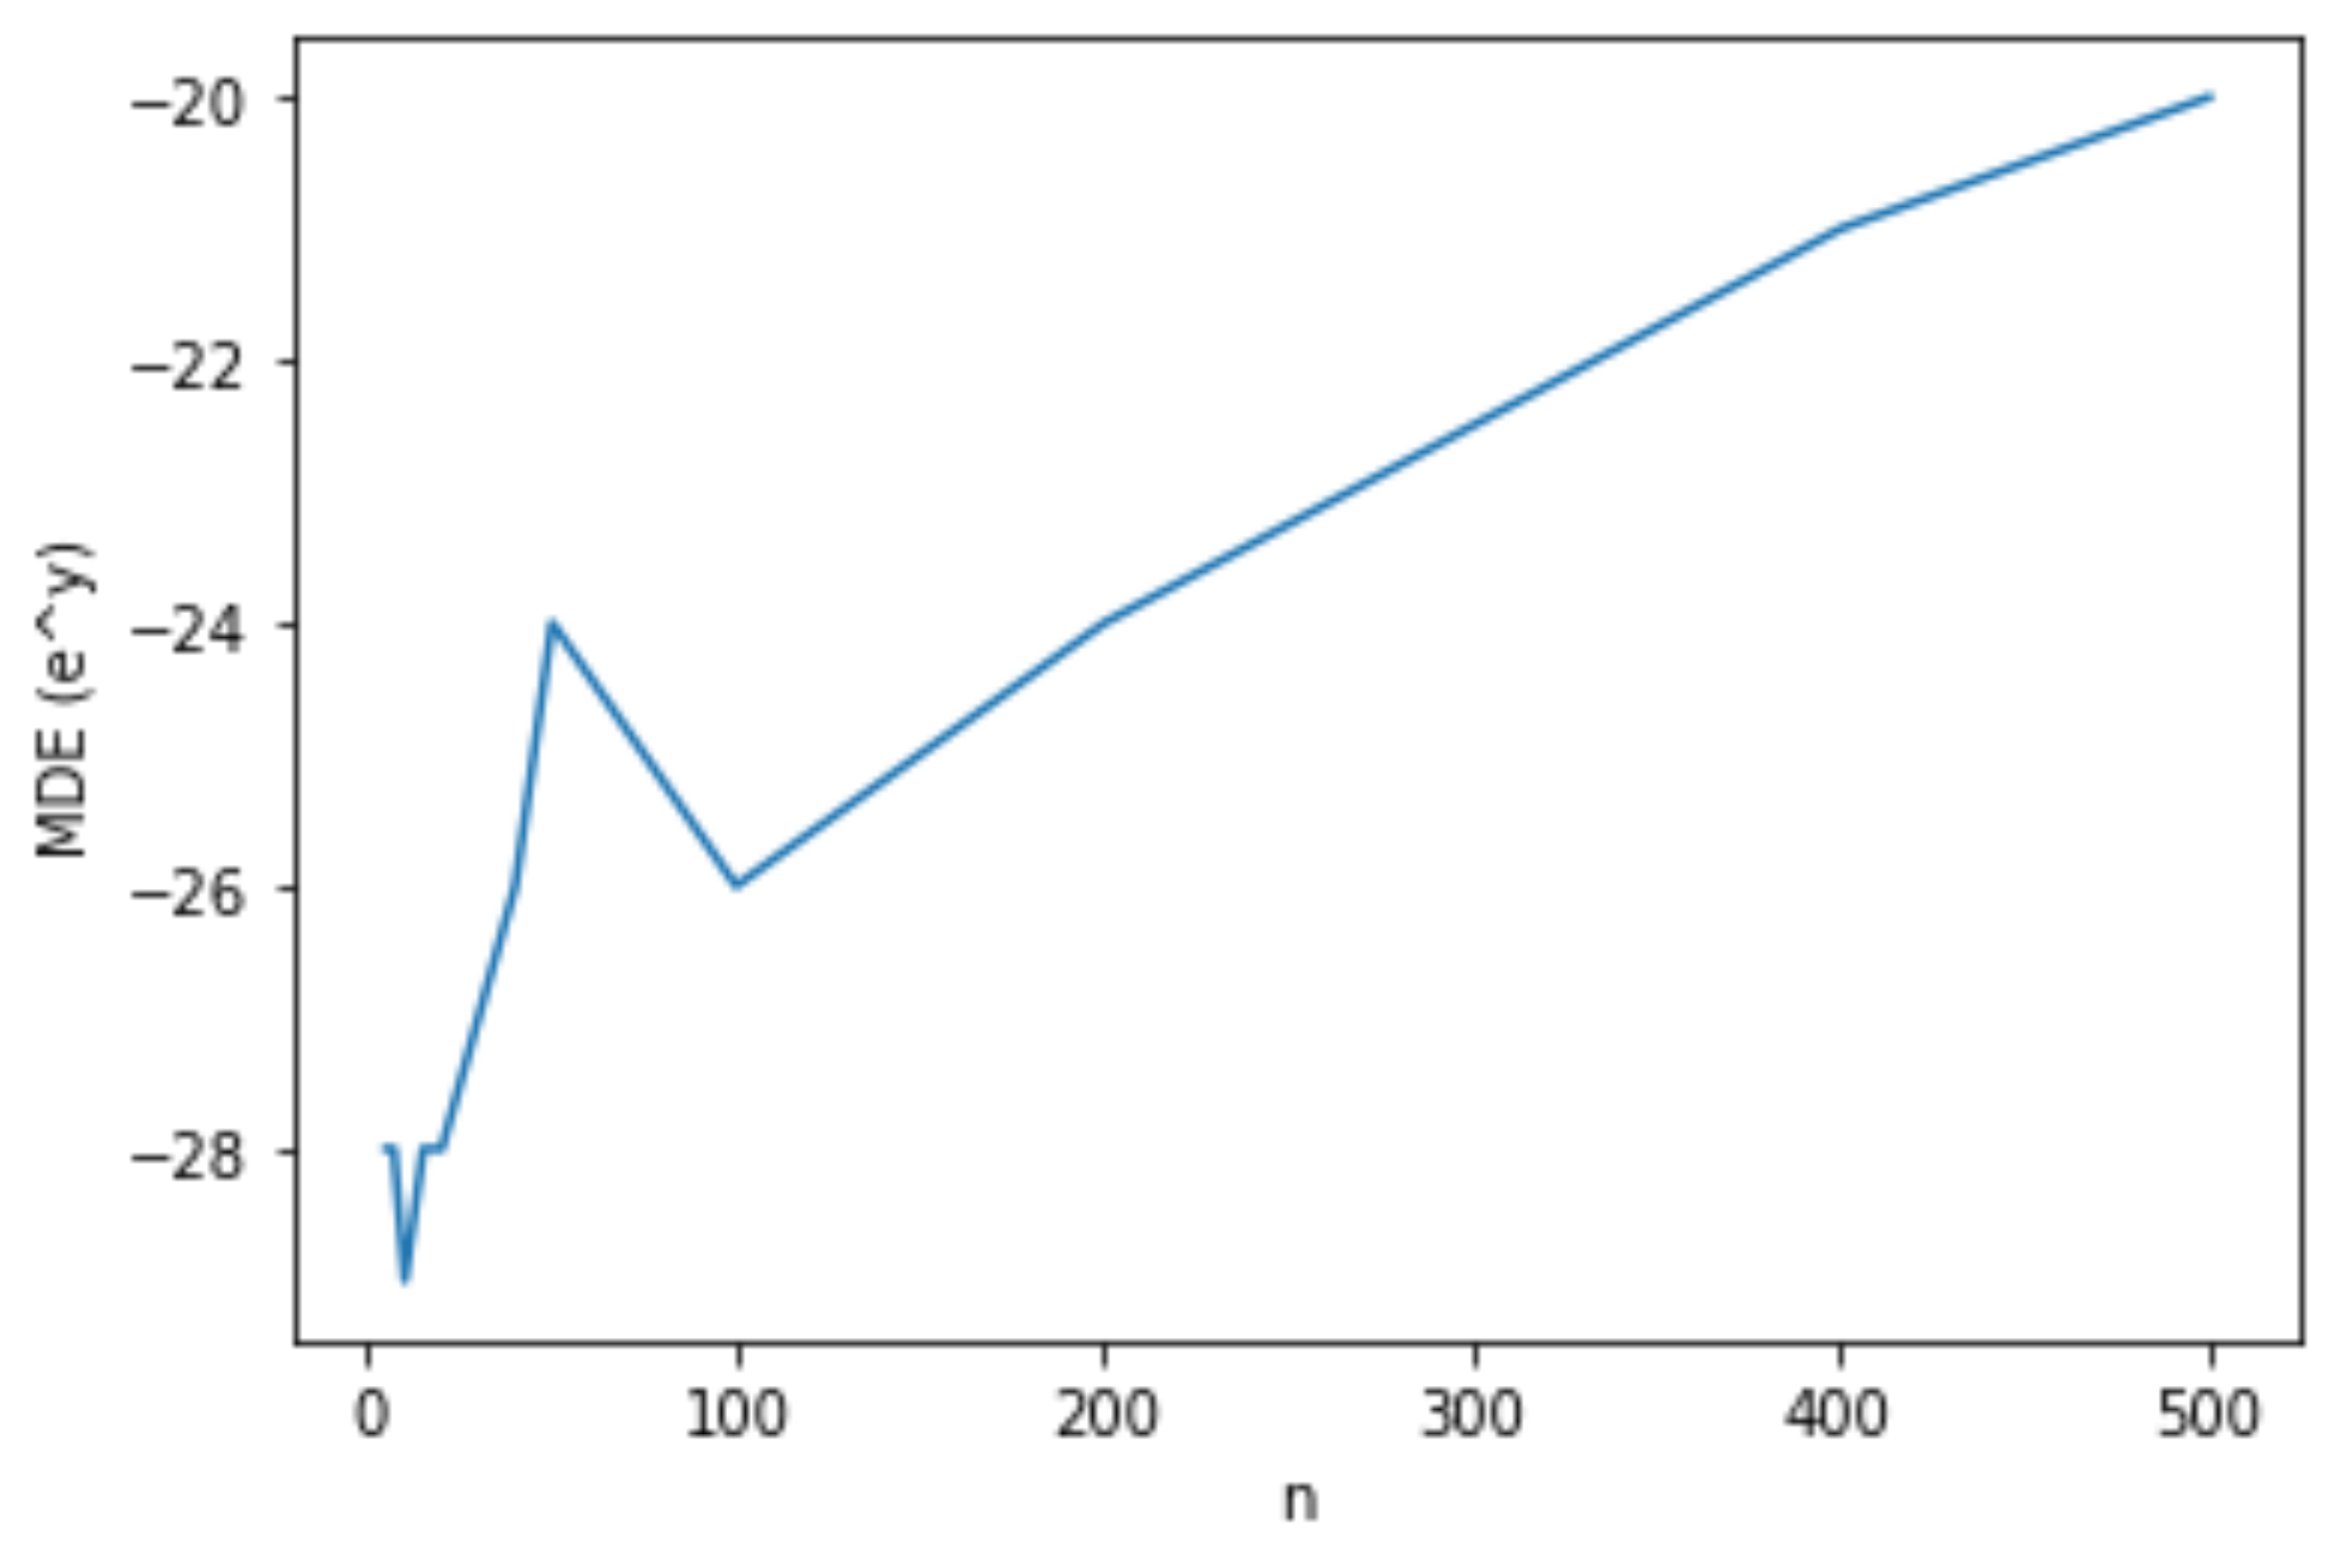
\includegraphics[width=1\linewidth]{figures/mdeTriPro.png}
					\end{center}
					\label{fig:mdeTri}
				\end{figure}
			\end{minipage}
		\end{center}
		\caption{A esquerda, o tempo de processo e, a direita, a ordem de grandeza associada ao MDE das soluções.}
		\label{fig:triPri}
	\end{figure}
	
	Também simulou-se o Algorítimo~\ref{alg:realizacaoTrilateration}, que teve um comportamento muito similar ao Algorítimo~\ref{alg:realizacaoIterativa}, como era de se esperar. Também usou-se instâncias $n$ variando em $\{5, 6, 7,10,15,20,30,40,50,100,200,400,500\}$. Porém, agora, com uma busca inteligente por vértices adjacentes, pode-se variar $\mathcal{P}$ afim de analisar diferentes geometrias para o problema, como apresenta-se a seguir.
	
	\subsubsection*{Instâncias com 70\% de arestas}
	
	\begin{figure}[H]
		\begin{center}
			\begin{minipage}{0.45 \linewidth}
				\begin{figure}[H]
					\begin{center}
						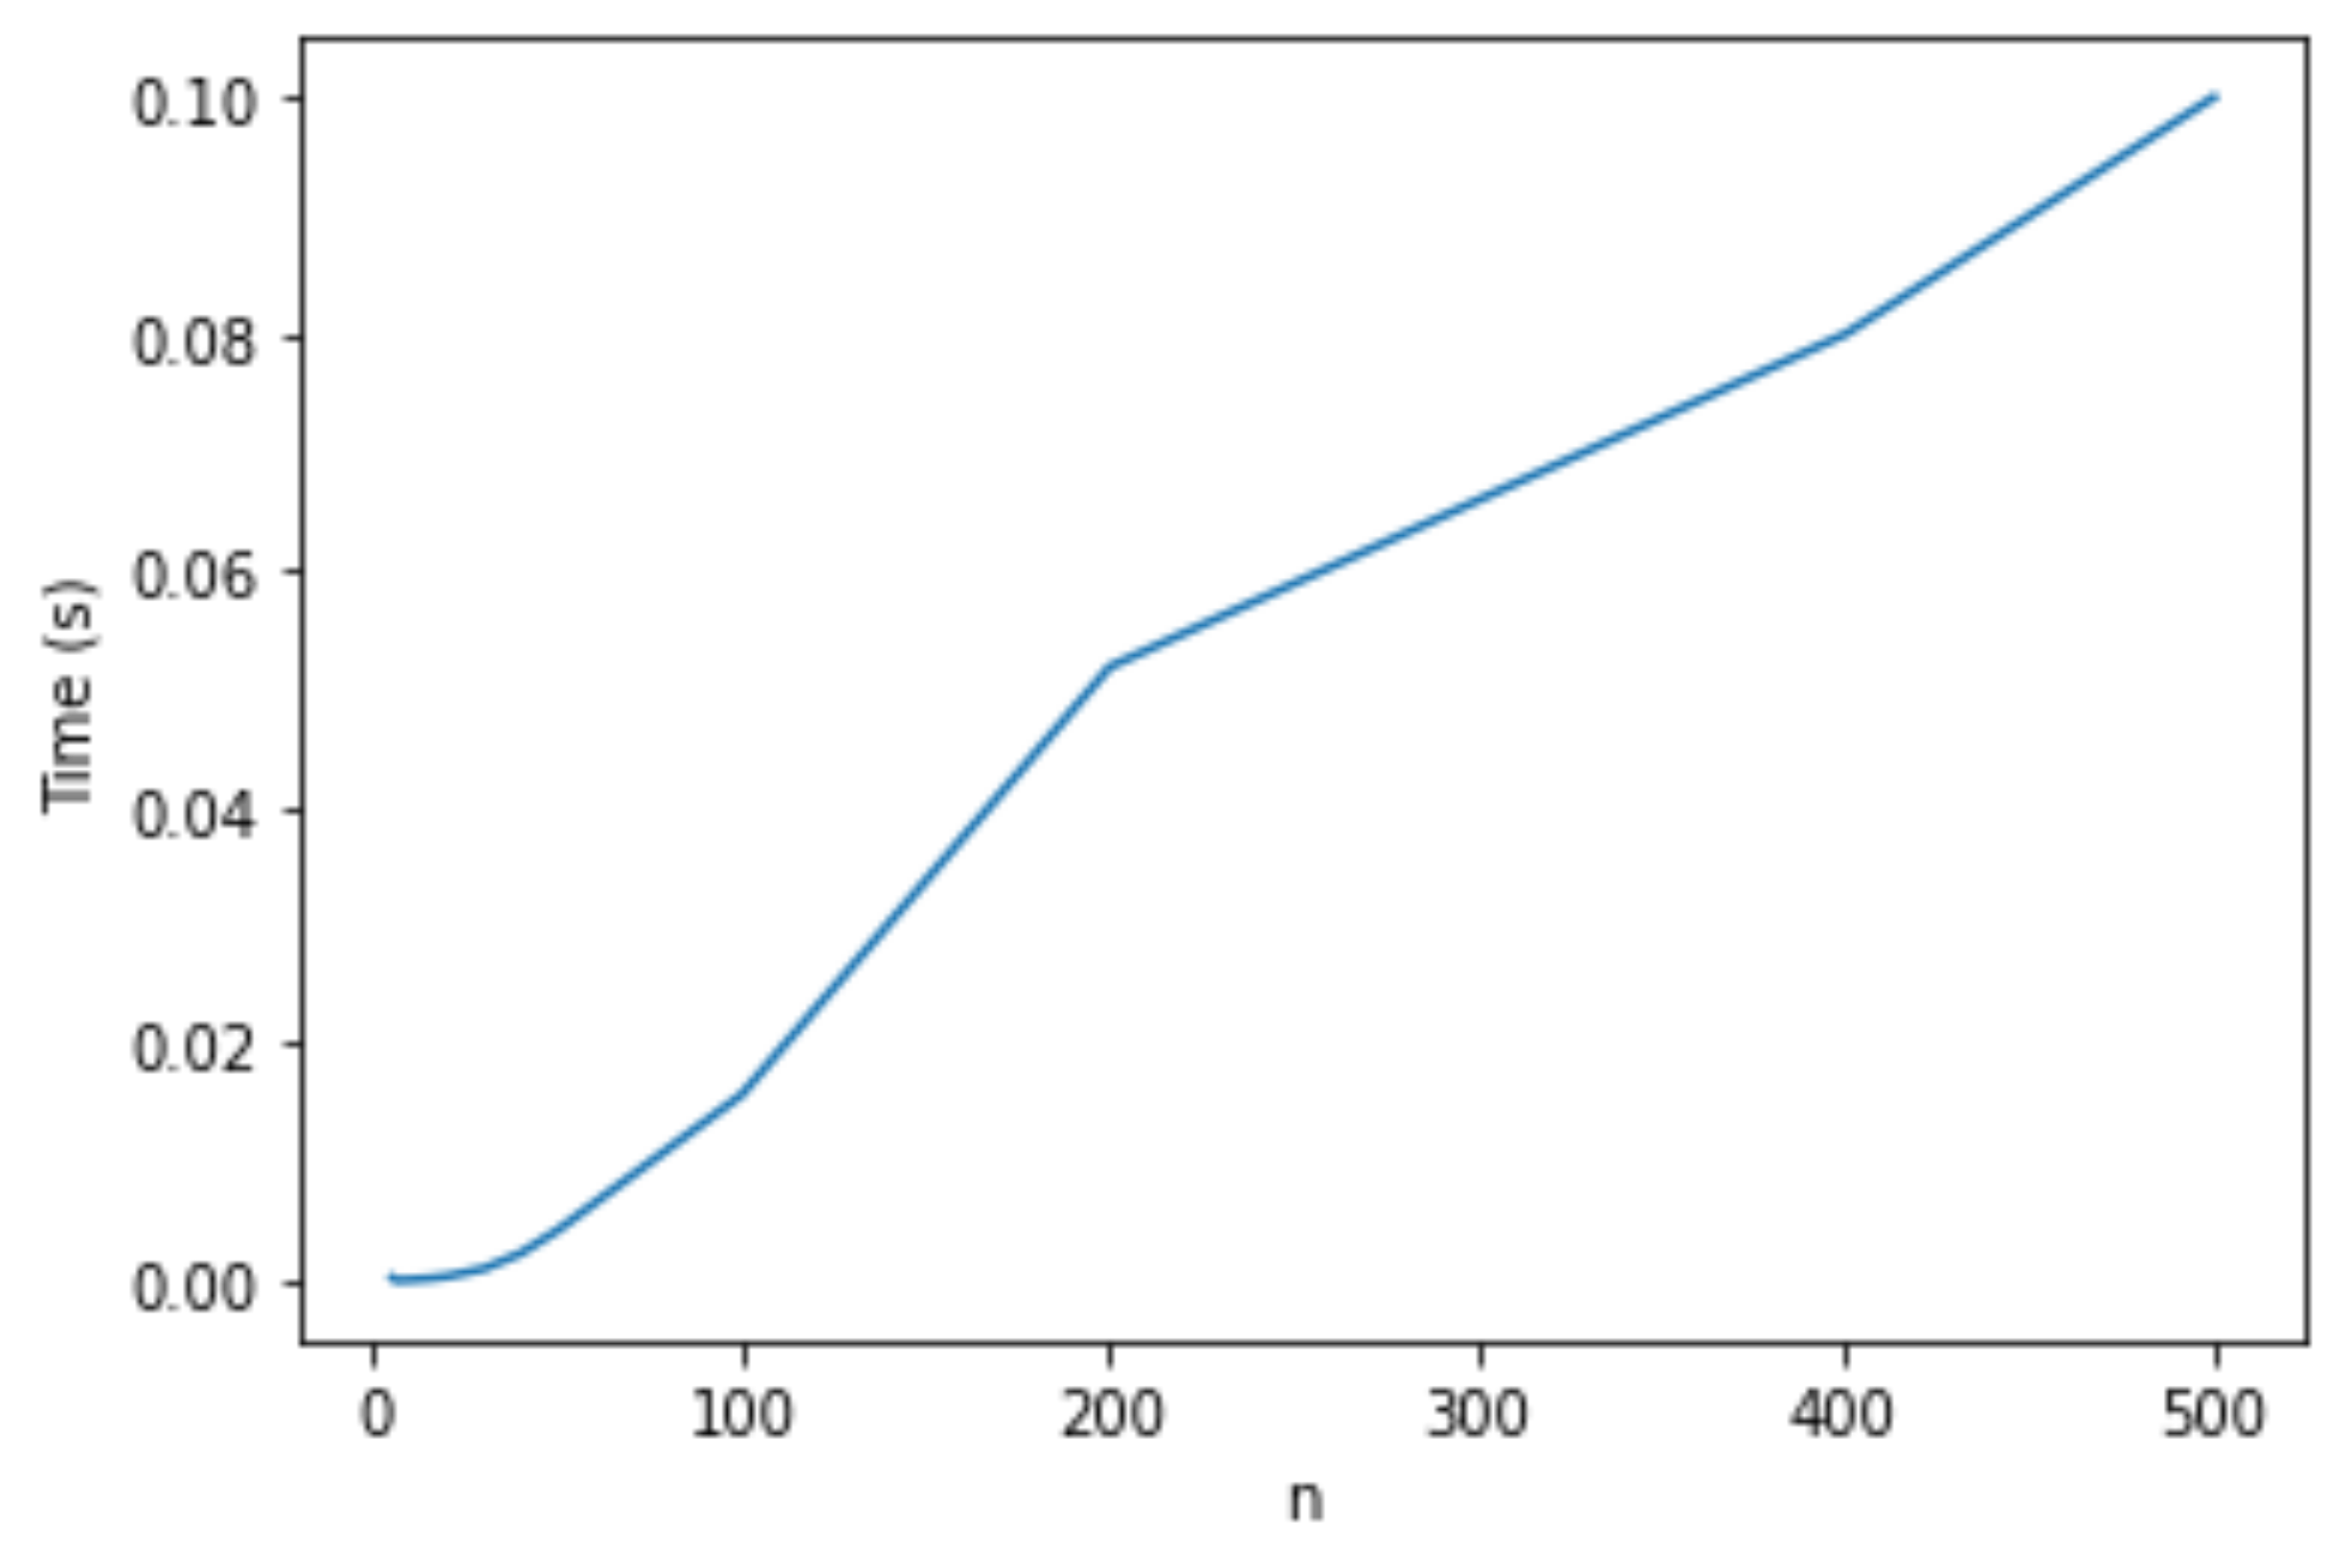
\includegraphics[width=1\linewidth]{figures/timeTriPro1.png}
					\end{center}
				\end{figure}
			\end{minipage}
			\hspace{0.1cm}
			\begin{minipage}{0.45 \linewidth}
				
				\begin{figure}[H]
					\begin{center}
						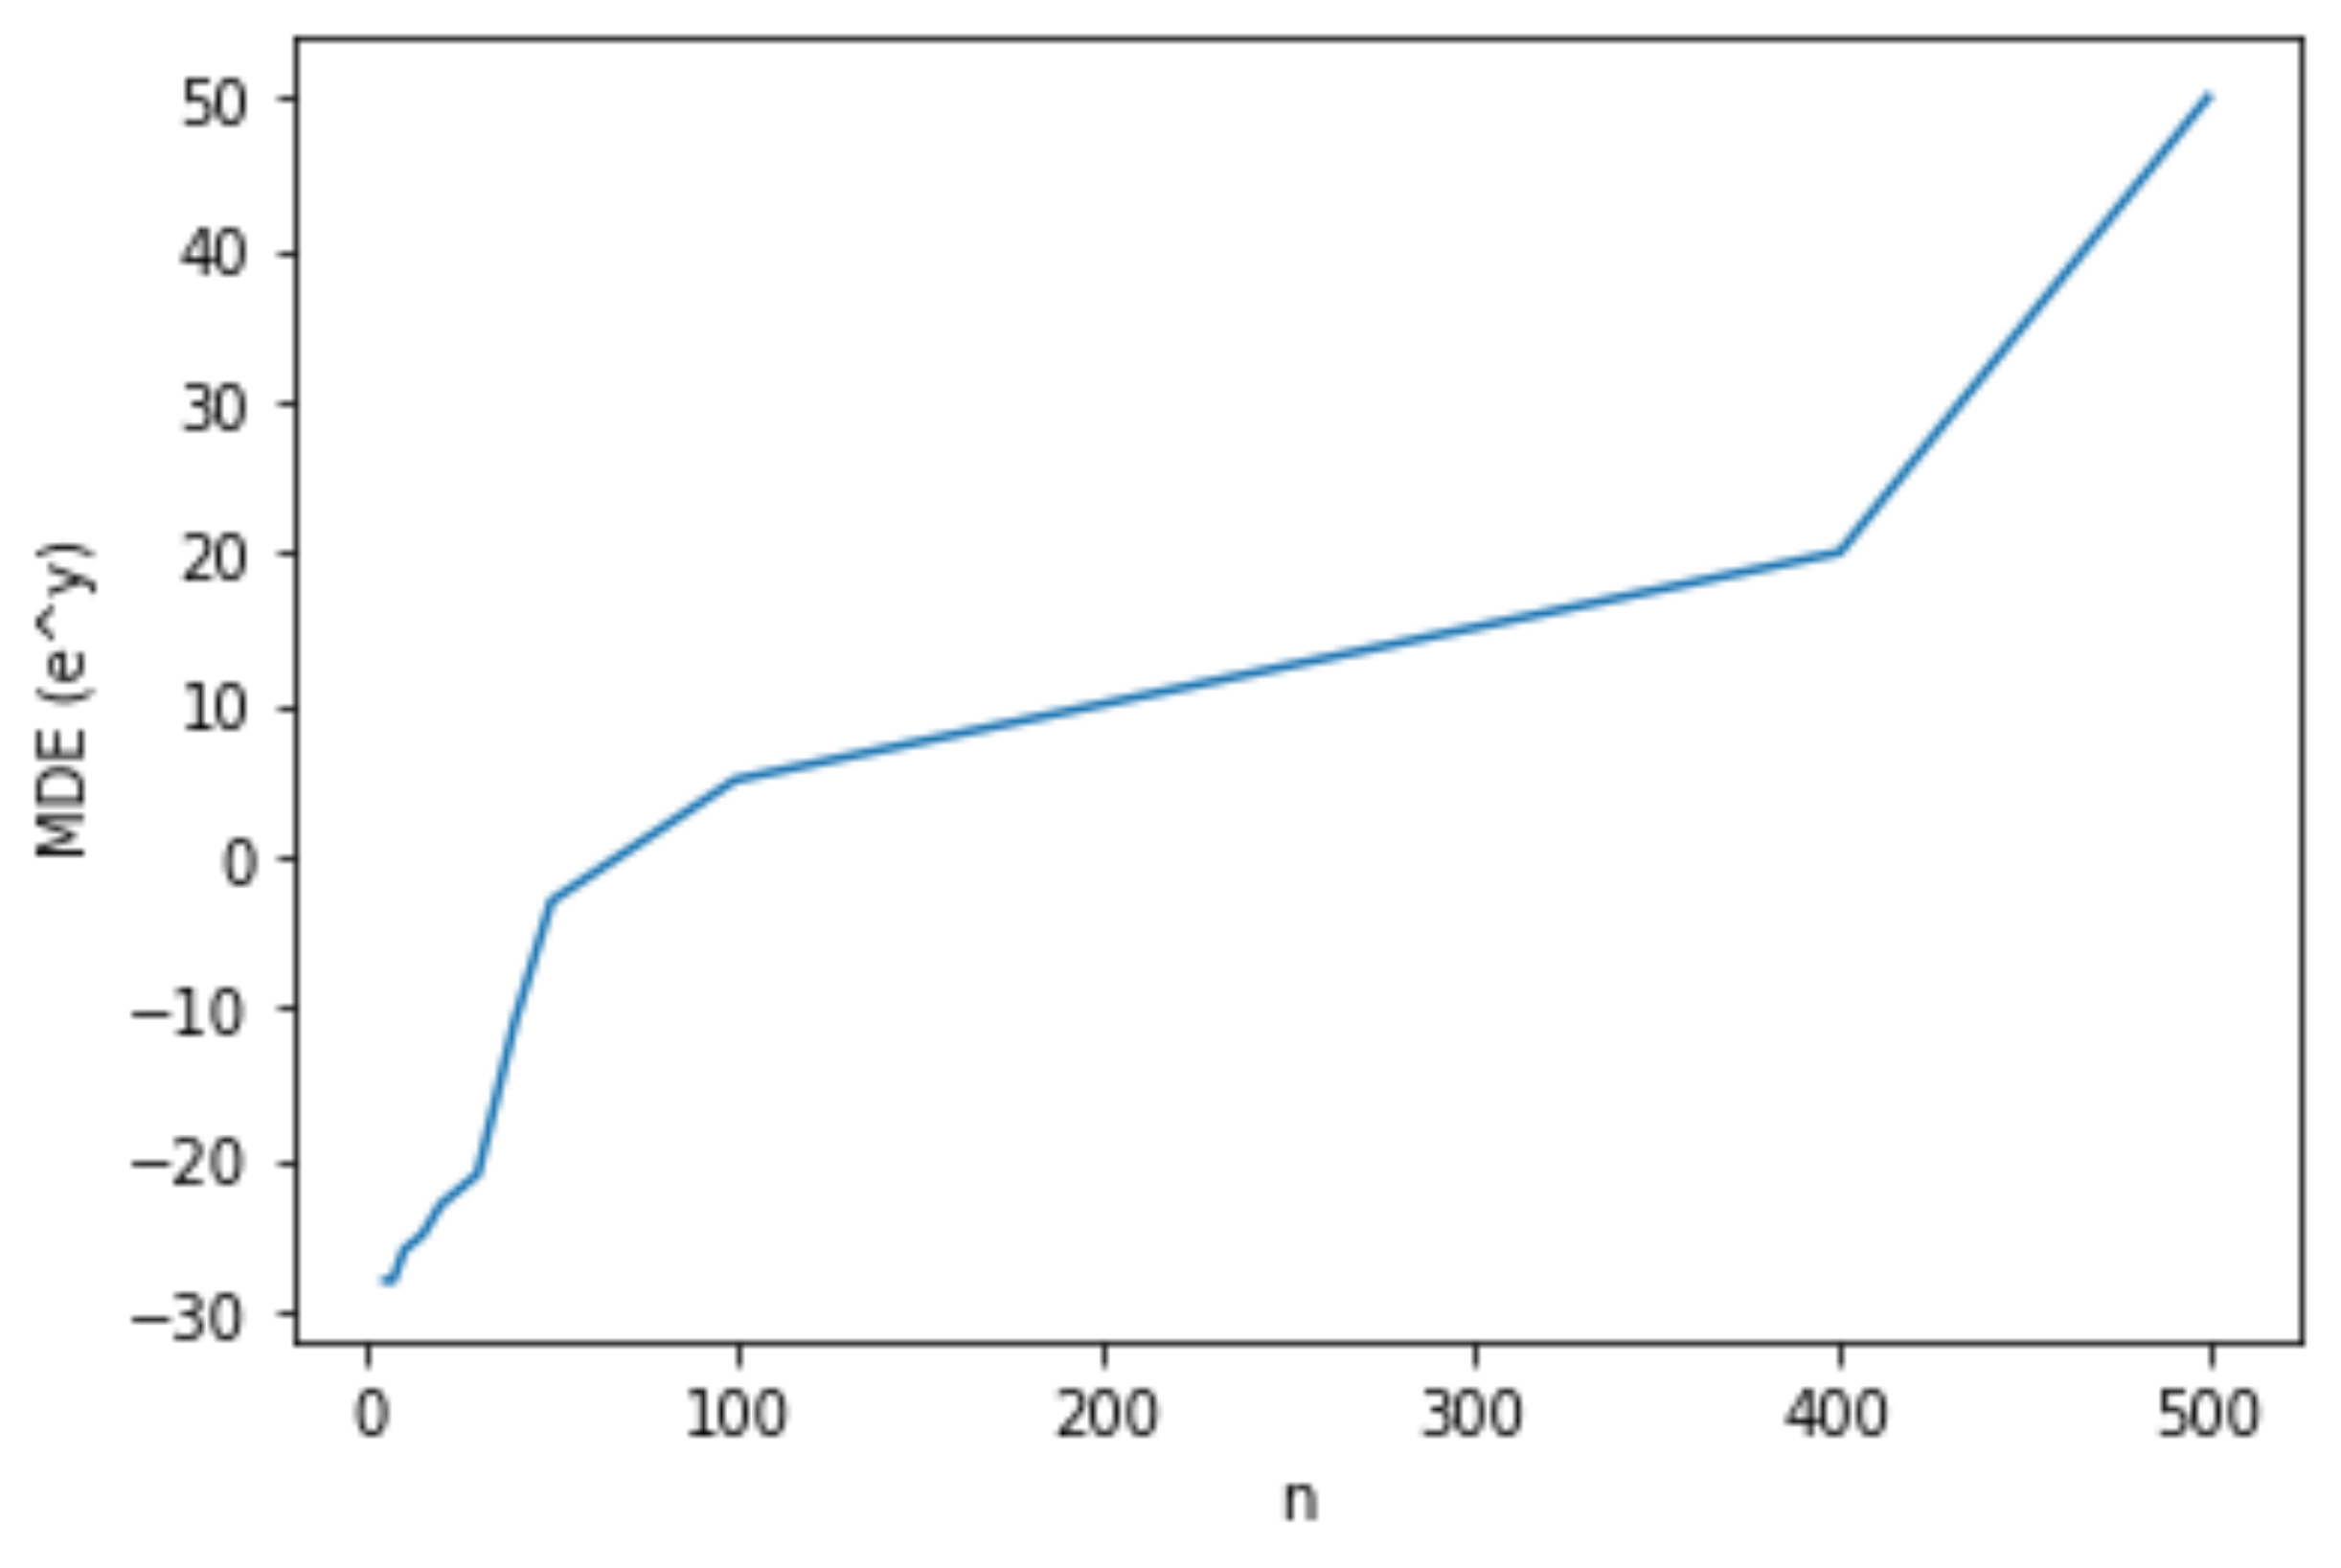
\includegraphics[width=1\linewidth]{figures/mdeTriPro1.png}
					\end{center}
					\label{fig:mdeTri}
				\end{figure}
			\end{minipage}
		\end{center}
		\caption{A esquerda, o tempo de processo e, a direita, a ordem de grandeza associada ao MDE das soluções. Utilizou-se $\mathcal{P} = 0.7$.}
		\label{fig:triPri4}
	\end{figure}
	
	\subsubsection*{Instâncias com 5\% de arestas}
	
	\begin{figure}[H]
		\begin{center}
			\begin{minipage}{0.45 \linewidth}
				\begin{figure}[H]
					\begin{center}
						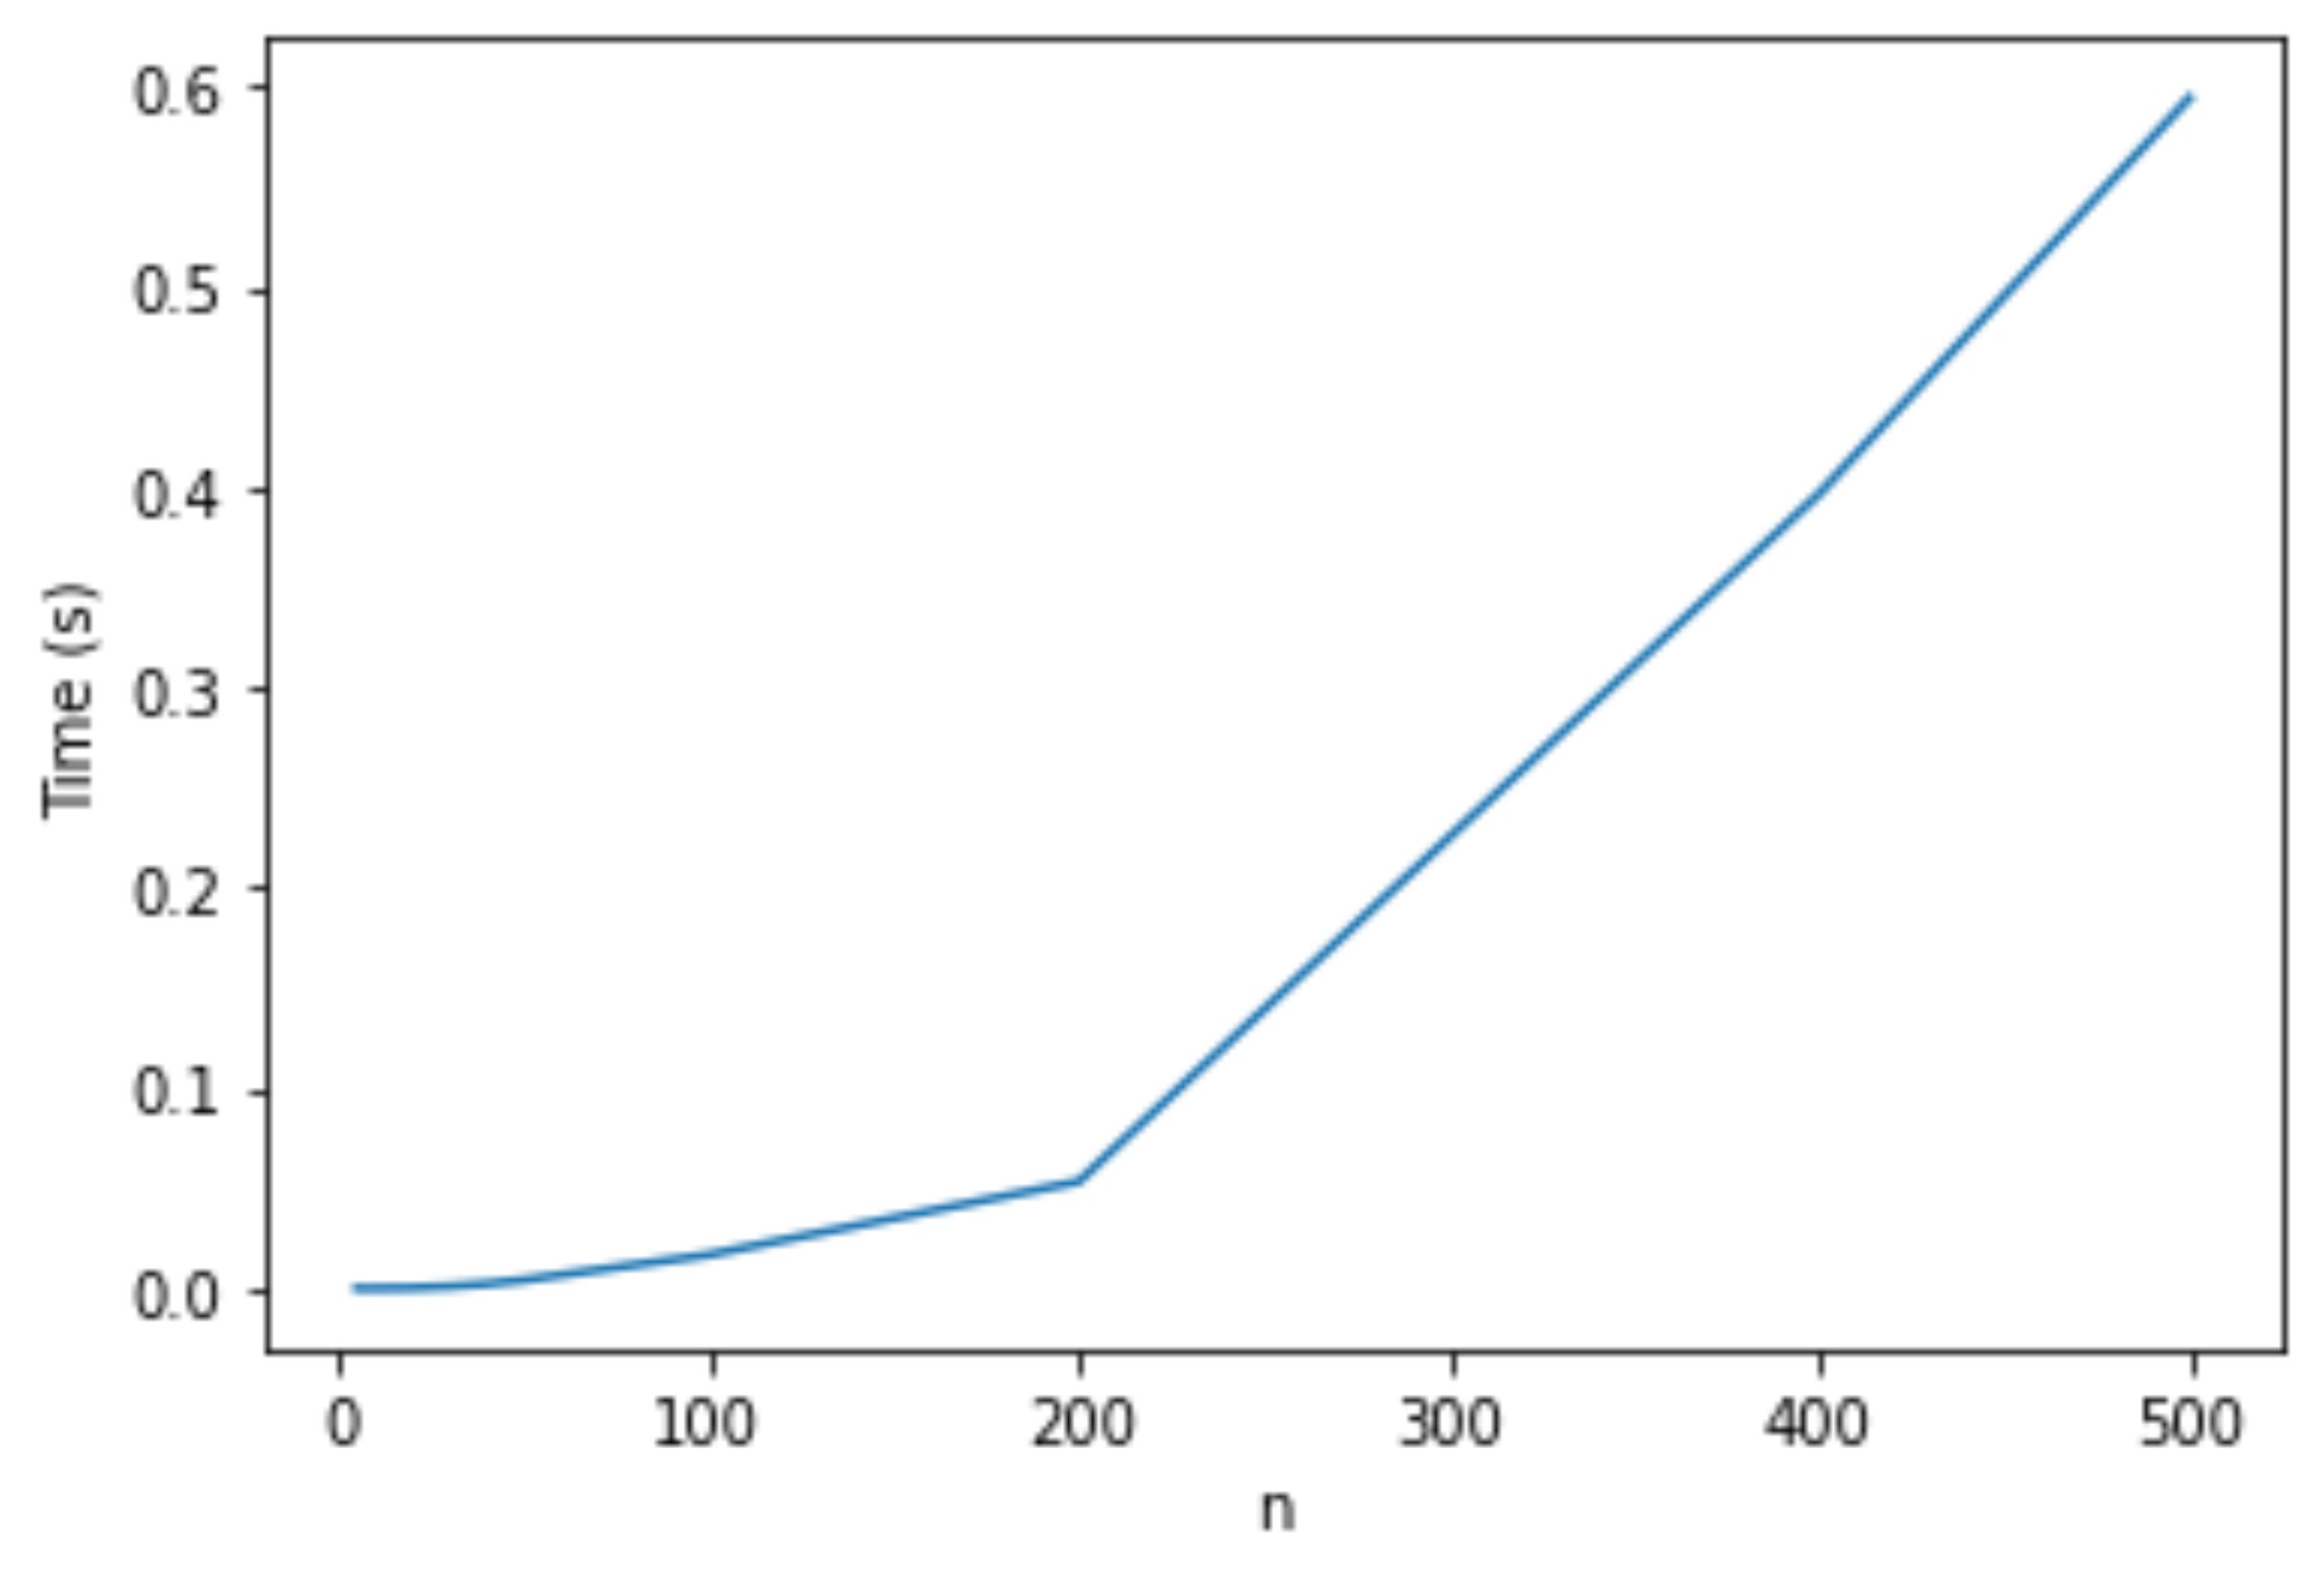
\includegraphics[width=1\linewidth]{figures/timePro2.png}
					\end{center}
				\end{figure}
			\end{minipage}
			\hspace{0.1cm}
			\begin{minipage}{0.45 \linewidth}
				
				\begin{figure}[H]
					\begin{center}
						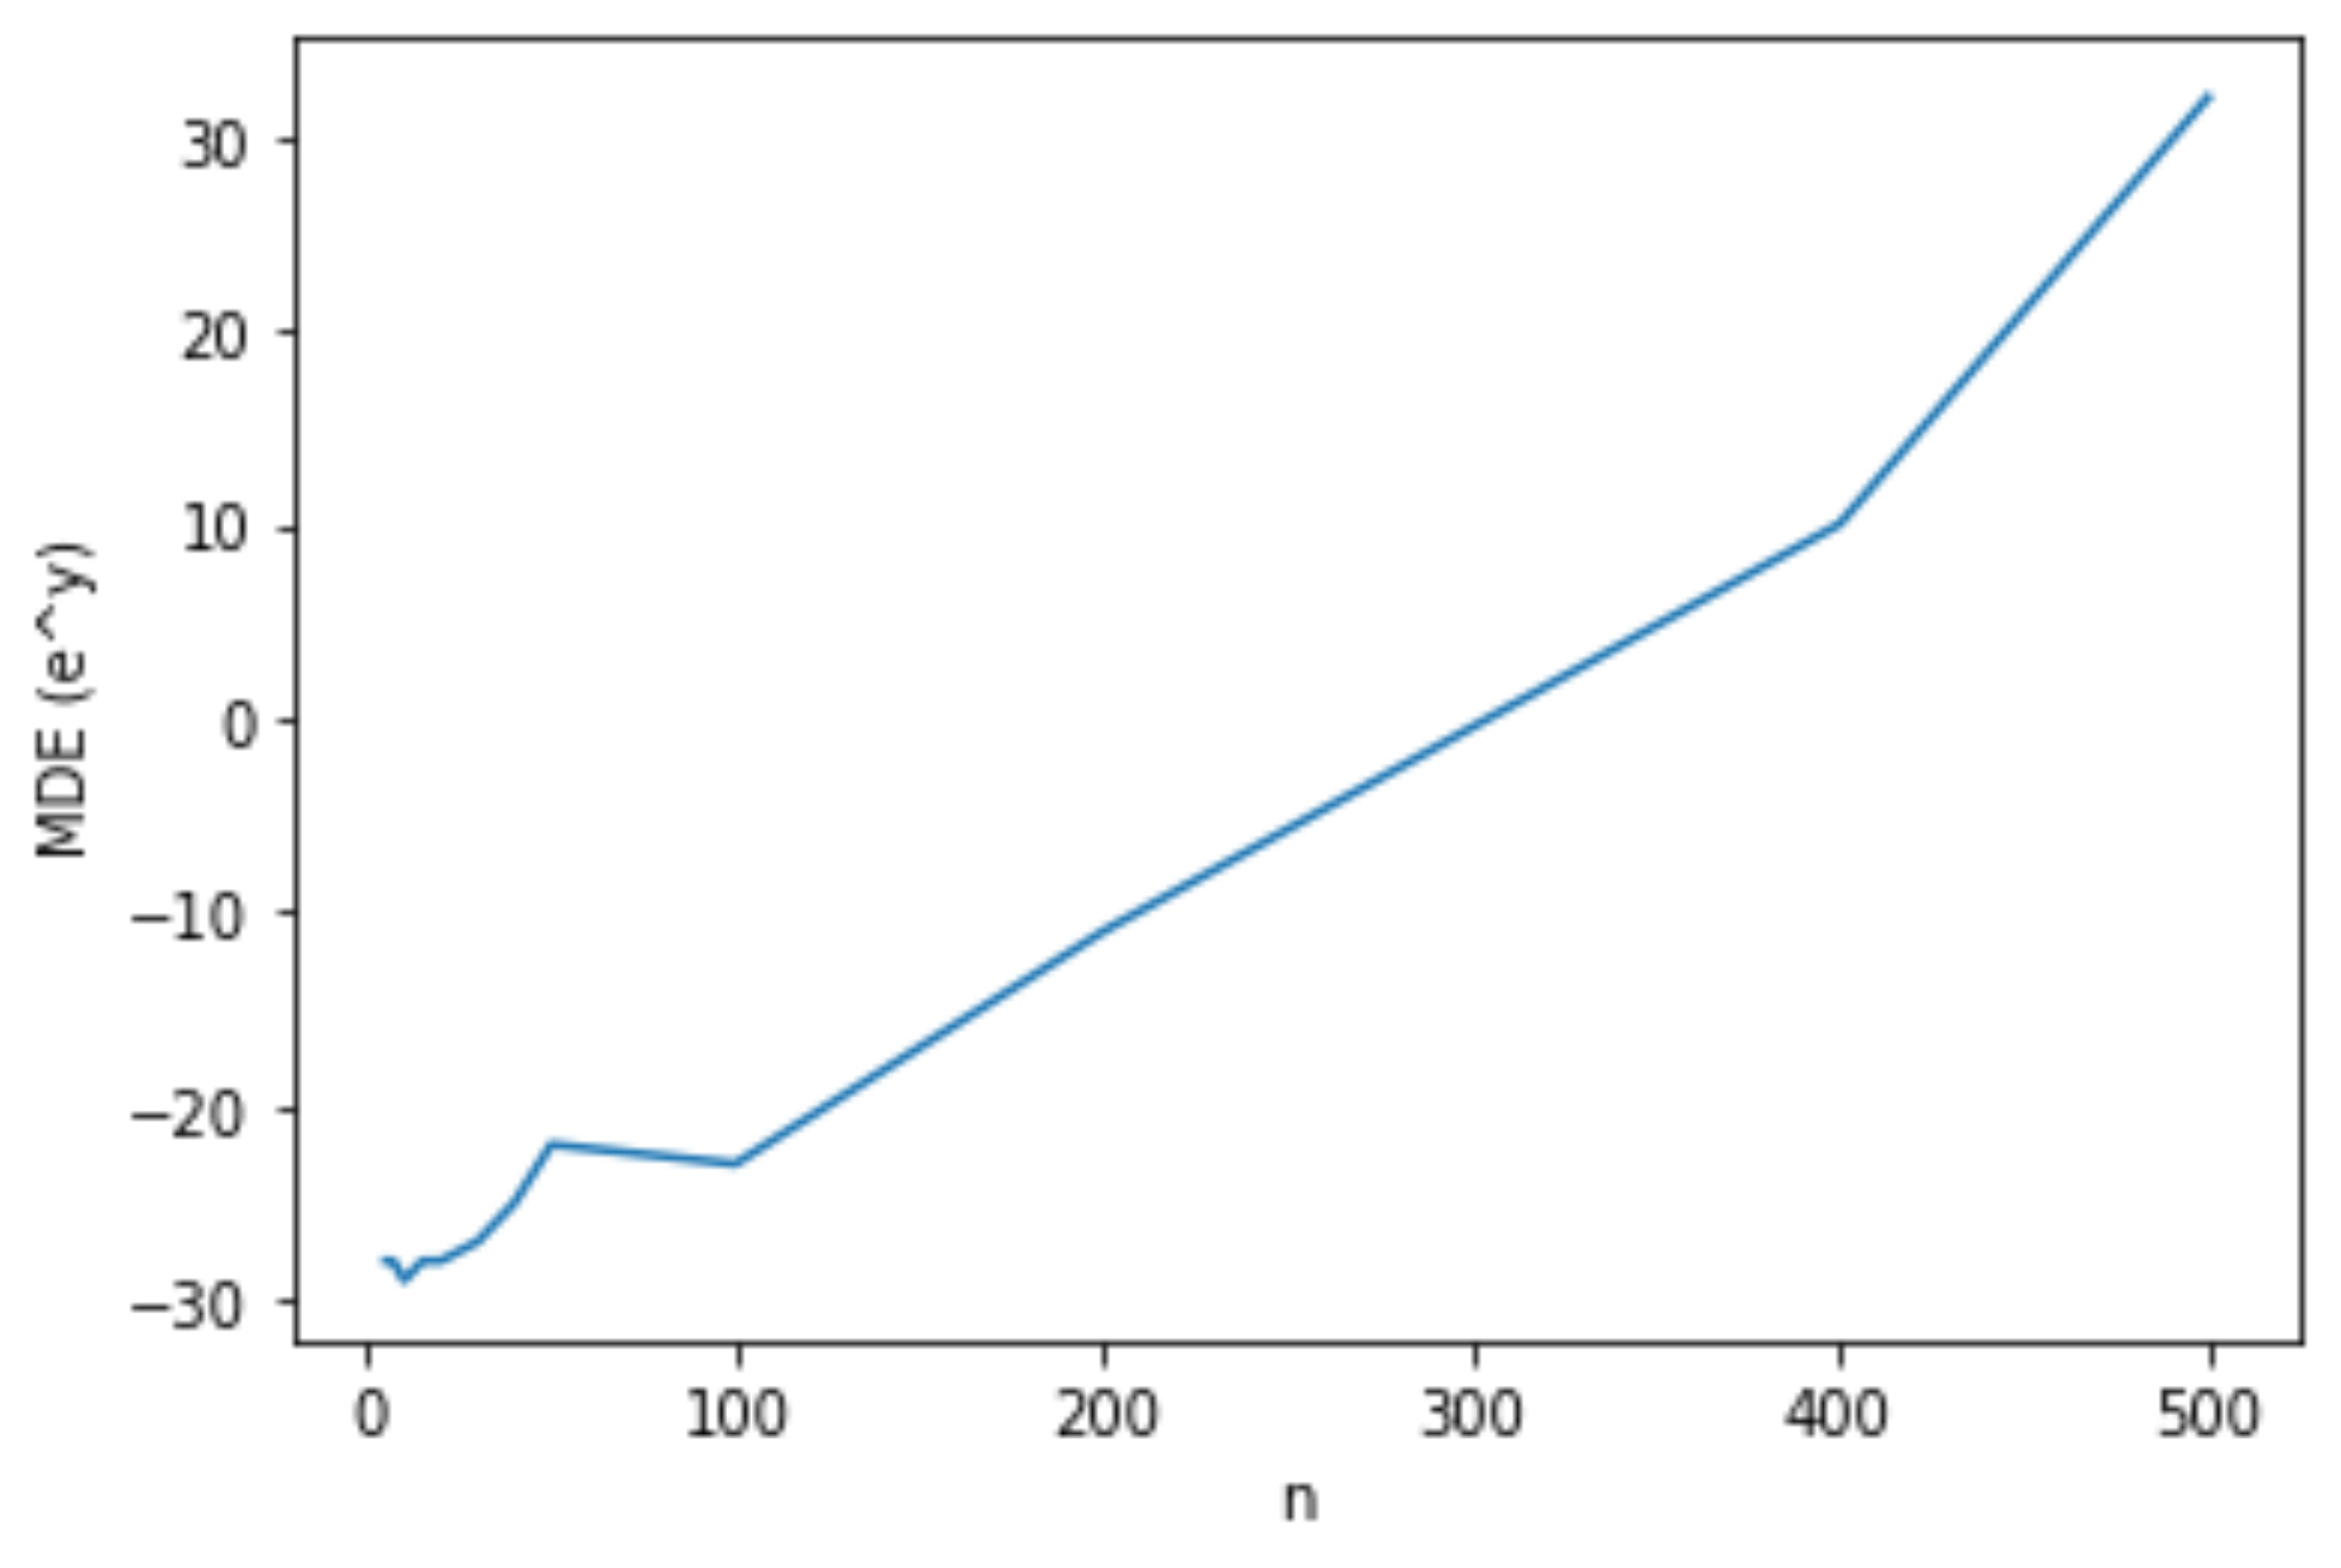
\includegraphics[width=1\linewidth]{figures/mdeTriPro2.png}
					\end{center}
					\label{fig:mdeTri}
				\end{figure}
			\end{minipage}
		\end{center}
		\caption{A esquerda, o tempo de processo e, a direita, a ordem de grandeza associada ao MDE das soluções. Utilizou-se $\mathcal{P} = 0.05$.}
		\label{fig:triPri3}
	\end{figure}
	
	Como esperado, é perceptível uma grande melhora na MDE das soluções conforme se diminui o valor de $\mathcal{P}$. 
	
	Também deve-se perceber que o tempo não obedeceu um padrão perfeito. Podemos relacionar esse fato com a aleatoriedade das instâncias, como pode-se notar que o Algoritmo~\ref{alg:realizacaoTrilateration} teve maios volatilidade no padrão temporal. Mesmo assim, há um consenso. As soluções mostradas nas Figuras~\ref{fig:triPri} e~\ref{fig:triPri3}, por exemplo, demonstram claramente um padrão polinomial, indo de encontro com o que foi apresentado na seção~\ref{sec:oi}.
	
	\newpage
	\section{Considerações Finais}
	Com isso, concluí-se o estudo sobre a Geometria de Distâncias aplicada ao problema de localização de sensores, tal qual teve como resultado um algorítimo que garante encontrar a solução do problema (se houver). .
	\\
	
	Nos cabe, nesse momento, voltarmos atenção às propostas levantadas internamente no início do projeto e verificar se elas foram cumpridas. Seguem o conjunto de objetivos específicos desse projeto, munidos de breve conclusão:
	
	\begin{enumerate}
		
		\item Estudar formas viáveis (pelos vieses energético, de construção e precisão da medida) para obtenção das distâncias entre os elementos do sistema físico:
		
		Fortemente embasado em \cite{savvides2001dynamic} e \cite{sensorsForMobileRobots}, faz-se uma apresentação sobre esses conceitos na Seção~\ref{sec:sensores}. 
		
		\item Estudar as possíveis distribuições dos Robôs Móveis em um sistema genérico, visando verificar quais conjuntos de dados possam ser garantidos como entradas para a construção do problema:
		
		Além de estudar distribuições genéricas, como em \cite{eren2004rigidity}, desenvolve-se na Seção~\ref{sec:disc} o Algorítimo~\ref{alg:instancia}, que cria instâncias aleatórias com diferentes densidades de ligações.
		
		\item Verificar a solução do Discretizable Order Problem \cite{carlileGDandAplications} aplicado ao problema proposto e estudar o ordenamento de vértices que se adeque aos objetivos do trabalho:
		
		Durante o desenvolvimento da Seção~\ref{sec:GD}, percebeu-se que uma ordem de discretização não seria necessária, visto que a definição do problema necessita de uma única solução \cite{libertiEDG}. Por conta disso, definiu-se a ordem de $K$-lateração, que garante a unicidade de solução.
		
		\item Caso consiga-se uma boa ordenação para os vértices, verificar a aplicação do algorítimo Branch-And-Prune \cite{carlile:BP} para a solução do problema proposto. Se não for possível, estudar outros algorítimos que possam solucionar o problema:
		
		Visto que o problema não era discreto, não fora possível aplicar o algorítimo Branch-And-Prune. Ao invés disso, se propôs o Algorítimo~\ref{alg:realizacaoTrilateration}, que utiliza a trilateração como núcleo e garante no máximo uma solução.
		
		\item Estudar a complexidade computacional do algorítimo proposto aplicado as possíveis distribuições:
		
		Isso foi feito no fim das Seções~\ref{sec:GD} e~\ref{sec:disc}, onde verificou-se que o algorítimo pode ser resolvido em tempo polinomial. Também mostrou-se um estudo sobre diferentes visões da geometria do problema afim de minimizar os erros associados. 
		
		\item Simular computacionalmente o algoritmo para solução do problema com instâncias artificialmente geradas, dominando cada passo utilizado:
		
		Simulações apresentadas, de forma satisfatória, na Seção~\ref{sec:disc}.
		
		\item Aplicar o algoritmo estudado em estruturas de pequena escala, como instâncias reais do problema:
		
		Não fora possível cumprir este último objetivo. Infelizmente, a manufatura de robôs móveis usando sensores de distância se demonstrou excessivamente custosa \cite{savvides2001dynamic, sensorsForMobileRobots}.
		
		Vale lembrar, porém, que a utilização de instâncias artificiais genéricas se mostrou de grande importância. Pode-se averiguar e discutir sobre diferentes geometrias, mesmo sem a prototipação de fato.
		
	\end{enumerate}
	
	Como experiências futuras, deseja-se estudar mais sobre a obtenção e tratamento de dados de distâncias, visto que esses possuem erros de medida \cite{sensorsForMobileRobots} (não levados em consideração nesse trabalho). Alguns trabalhos relacionados à Geometria de Distâncias aplicada ao caso intervalar são mostrados em \cite{wsnlSemidefinitePrograming}. Há curiosidade em ver como medida MDE se comporta para uma quantidade grande de vértices associados a erros de medida.
	
	Também deseja-se fazer estudos sobre geometrias mínimas para o problema, como feito em \cite{wsnlFewAnchors}. Deseja-se verificar um conjunto de condições que restringem o movimento de um robô móvel afim de garantir que este ainda possa ser localizado.
	
	\newpage
	\phantomsection
	\addcontentsline{toc}{section}{Referências}
	
	\bibliographystyle{unsrt}
	\bibliography{references}
	
	\newpage
	\appendix
	\input{secGD/apendices.tex}

\end{document}

	
	\newpage
	
	 \documentclass[a4paper,12pt]{article}
\usepackage[a4paper,top=3cm,bottom=2cm,left=3cm,right=3cm,marginparwidth=1.75cm]{geometry}
\usepackage[brazil]{babel}
\usepackage[T1]{fontenc}
\usepackage[utf8]{inputenc}
\usepackage{amsmath}
\usepackage{MnSymbol}
\usepackage{wasysym}
\usepackage{hyperref}
\usepackage{color}
\definecolor{Blue}{rgb}{0,0,0.9}
\definecolor{Red}{rgb}{0.9,0,0}
\usepackage{esvect}
\usepackage{graphicx}
\usepackage{float}
\usepackage{indentfirst}
\usepackage{caption}
\usepackage{blkarray}
\newcommand\Mark[1]{\textsuperscript#1}
\usepackage{pgfplots}
\usepackage{amsfonts}
\usepackage[english, ruled, linesnumbered]{algorithm2e}
\usepackage{algorithmic}
\newtheorem{definicao}{Definição}[section]
\newtheorem{teorema}{Teorema}[section]

\title{Disposição de Robôs Móveis no espaço Euclidiano 3D: uma aplicação de Geometria de Distâncias}
\author{Guilherme Philippi\Mark{*}, orientado por Felipe Delfini Caetano Fidalgo\Mark{\dagger}\\Campus Blumenau\\Universidade Federal de Santa Catarina\\UFSC
	\\guilherme.philippi@grad.ufsc.br\Mark{*}, felipe.fidalgo@ufsc.br\Mark{\dagger}}
\begin{document}
	\begin{titlepage}
		\newcommand{\HRule}{\rule{\linewidth}{0.5mm}} % Defines a new command for the horizontal lines, change thickness here
		\center % Center everything on the page
		%----------------------------------------------------------------------------------------
		%	HEADING SECTIONS
		%----------------------------------------------------------------------------------------
		\begin{center}
			
\includegraphics[scale=0.22]{figures/logoufsc.jpg}
		\end{center}
		\vspace{1cm}
		
		\textsc{\LARGE \hspace{-0.17cm}Universidade Federal de Santa Catarina}\\[0.5cm] % Name of your university/college
		{\Large Centro de Blumenau \\ Departamento de Matemática}\\[1.5cm] % Major heading such as course name
		\textsc{\Large PIBIC \\ Relatório Final \vspace{1.5cm}  \\ }{\large Geometria de Distâncias e Álgebras Geométricas: novas perspectivas geométricas, computacionais e aplicações}\\[2.0cm] % Minor heading such as course title
		
		%\textsc{\LARGE Universidade Federal de Santa Catarina}\\[0.5cm] % Name of your university/college
		%{\Large Centro de Blumenau \\ Departamento de Matemática}\\[1.5cm] % Major heading such as course name
		%\textsc{\Large PIBIC \\ Programa Institucional de Bolsas de Iniciação Científica \vspace{1.5cm} \\ {\bf PROJETO DE PESQUISA}}\\[2.0cm] % Minor heading such as course title
		
		%----------------------------------------------------------------------------------------
		%	TITLE SECTION
		%----------------------------------------------------------------------------------------
		
		\HRule \\[0.4cm]
		{ \LARGE \bfseries \textbf{Disposição de Robôs Móveis no espaço Euclidiano 3D: uma aplicação de Geometria de Distâncias}} \\ [0.4cm] % Title of your document
		\HRule \\[2cm]
		
		%----------------------------------------------------------------------------------------
		%	AUTHOR SECTION
		%----------------------------------------------------------------------------------------
		
		\begin{minipage}{1\textwidth}
			\begin{center} \large
				Guilherme Philippi (g.philippi@grad.ufsc.br),
				\vspace{0.5cm}
				\\
				\underline{\textsc{Orientador:}} \vspace{0.2cm}
				Felipe Delfini Caetano Fidalgo (felipe.fidalgo@ufsc.br).
			\end{center}
		\end{minipage} \\[2cm]
		
		
		{\large \today} % Date, change the \today to a set date if you want to be precise
		
		
		\vfill % Fill the rest of the page with whitespace
		
	\end{titlepage}
	
	
	\newpage
	\vspace{-1cm}
	\tableofcontents
	\newpage
	
	\begin{center}
		\large
		\textbf{Abstract}
	\end{center}
	
	
	In this work, the Distance Geometry Problem Trilaterative applied to the sensor location problem was studied, as well as the necessary tools for its understanding, going from graph theory to the characteristics of systems involving mobile robotics. An overview of Geometry of Distances was presented, which enabled the correct definition of the problem and polynomial algorithms to solve it. The text ends with an analysis of computer simulations of the problem, using different geometries, as well as an algorithm to generate them.
	
	\textbf{Keywords:} TDGP, Distance Geometry, Mobile Robotics.
	
	
	\vspace{2cm}	
	\begin{center}
		\large
		\textbf{Resumo}
	\end{center}
	
	Neste trabalho, foram estudados o Trilaterativo Distance Geometry Problem aplicado ao problema de localização de sensores, bem como as ferramentas necessárias para sua compreensão, passando da teoria de grafos às características de sistemas envolvendo robótica móvel. Apresentou-se uma visão geral de Geometria de Distâncias que possibilitou a correta definição do problema e de algorítimos polinomiais para solucioná-lo. O texto se encerra com uma analise de simulações computacionais do problema, utilizando diferentes geometrias, bem como um algorítimo para gerá-las. 
	
	\textbf{Palavras-chave:} TDGP, Geometria de Distâncias, Robótica Móvel.
	
	
	\newpage
	\section{Introdução}
	
	Percebe-se uma tendencia de mercado em se adotar sistemas autônomos móveis para realizar funções que dependem de um grande número de maquinas, como o controle do estoque em um armazém, um sistema de entrega ou o cultivo e tratamento de grandes áreas de plantio \cite{mobileRobotsCook}. O estudo da localização de robôs móveis é vasta na literatura \cite{eren2004rigidity, mobileRobotsTzafestas}, o que demonstra a importância deste tema. Qualquer solução de engenharia móvel, seja autônoma ou não, precisa definir uma forma de localizar seu objeto de estudo. Por conta disso, ao decorrer desse texto apresenta-se soluções envolvendo Geometria de Distâncias como alternativas para a obtenção de localização.
	\\
	
	A Geometria de Distâncias (GD) é uma matéria de interesse relativamente recente da Ciência \cite{carlileGDandAplications}, disposta em uma vasta interseção entre diversas áreas do conhecimento. Em suma, ela se preocupa com os aspectos geométricos decorrentes dos objetos que estão dispostos em algum espaço e possuam uma relação de distância medível, advindas de origens tão variáveis quanto se queira. Como é o caso de estudo deste texto: distâncias entre robôs móveis com seu meio e, em particular, outros robôs móveis.
	\\
	
	Para poder relacionar esses distâncias, no que se segue, apresenta-se um estudo sobre a Teoria de Grafos (Seção~\ref{sec:grafos}), que demonstrou-se uma ferramenta importante para GD --- em contraponto à antiga utilização de matrizes de distâncias \cite{carlileGDandAplications}. A seguir, por tanto, na Seção~\ref{sec:GD}, desenvolve-se o problema fundamental deste trabalho a partir da definição de Grafos e faz-se um estudo sobre algorítimos descritos na literatura para solucioná-lo. Na Seção~\ref{sec:robos}, faz-se uma introdução a robótica móvel e apresenta-se um estudo sobre sensoriamento. 
	
	O trabalho se encerra com algumas simulações computacionais do problema, na Seção~\ref{sec:disc}, além de discussões envolvendo esses resultados. O texto também contém dois apêndices, podendo serem usados como consulta, caracterizando algumas ferramentas matemáticas utilizadas. 
	\\
	
	A revisão bibliográfica completa pode ser encontrada no fim do documento, sendo devidamente citada durante o texto. 
	
	\newpage
	
	\phantomsection
	\addcontentsline{toc}{section}{Materiais e Métodos}
	\section*{Materiais e Métodos}
	No que se segue, apresenta-se o estudo desenvolvido neste trabalho.
	
	 \documentclass[a4paper,12pt]{article}
\usepackage[a4paper,top=3cm,bottom=2cm,left=3cm,right=3cm,marginparwidth=1.75cm]{geometry}
\usepackage[brazil]{babel}
\usepackage[T1]{fontenc}
\usepackage[utf8]{inputenc}
\usepackage{amsmath}
\usepackage{MnSymbol}
\usepackage{wasysym}
\usepackage{hyperref}
\usepackage{color}
\definecolor{Blue}{rgb}{0,0,0.9}
\definecolor{Red}{rgb}{0.9,0,0}
\usepackage{esvect}
\usepackage{graphicx}
\usepackage{float}
\usepackage{indentfirst}
\usepackage{caption}
\usepackage{blkarray}
\newcommand\Mark[1]{\textsuperscript#1}
\usepackage{pgfplots}
\usepackage{amsfonts}
\usepackage[english, ruled, linesnumbered]{algorithm2e}
\usepackage{algorithmic}
\newtheorem{definicao}{Definição}[section]
\newtheorem{teorema}{Teorema}[section]

\title{Disposição de Robôs Móveis no espaço Euclidiano 3D: uma aplicação de Geometria de Distâncias}
\author{Guilherme Philippi\Mark{*}, orientado por Felipe Delfini Caetano Fidalgo\Mark{\dagger}\\Campus Blumenau\\Universidade Federal de Santa Catarina\\UFSC
	\\guilherme.philippi@grad.ufsc.br\Mark{*}, felipe.fidalgo@ufsc.br\Mark{\dagger}}
\begin{document}
	\begin{titlepage}
		\newcommand{\HRule}{\rule{\linewidth}{0.5mm}} % Defines a new command for the horizontal lines, change thickness here
		\center % Center everything on the page
		%----------------------------------------------------------------------------------------
		%	HEADING SECTIONS
		%----------------------------------------------------------------------------------------
		\begin{center}
			
\includegraphics[scale=0.22]{figures/logoufsc.jpg}
		\end{center}
		\vspace{1cm}
		
		\textsc{\LARGE \hspace{-0.17cm}Universidade Federal de Santa Catarina}\\[0.5cm] % Name of your university/college
		{\Large Centro de Blumenau \\ Departamento de Matemática}\\[1.5cm] % Major heading such as course name
		\textsc{\Large PIBIC \\ Relatório Final \vspace{1.5cm}  \\ }{\large Geometria de Distâncias e Álgebras Geométricas: novas perspectivas geométricas, computacionais e aplicações}\\[2.0cm] % Minor heading such as course title
		
		%\textsc{\LARGE Universidade Federal de Santa Catarina}\\[0.5cm] % Name of your university/college
		%{\Large Centro de Blumenau \\ Departamento de Matemática}\\[1.5cm] % Major heading such as course name
		%\textsc{\Large PIBIC \\ Programa Institucional de Bolsas de Iniciação Científica \vspace{1.5cm} \\ {\bf PROJETO DE PESQUISA}}\\[2.0cm] % Minor heading such as course title
		
		%----------------------------------------------------------------------------------------
		%	TITLE SECTION
		%----------------------------------------------------------------------------------------
		
		\HRule \\[0.4cm]
		{ \LARGE \bfseries \textbf{Disposição de Robôs Móveis no espaço Euclidiano 3D: uma aplicação de Geometria de Distâncias}} \\ [0.4cm] % Title of your document
		\HRule \\[2cm]
		
		%----------------------------------------------------------------------------------------
		%	AUTHOR SECTION
		%----------------------------------------------------------------------------------------
		
		\begin{minipage}{1\textwidth}
			\begin{center} \large
				Guilherme Philippi (g.philippi@grad.ufsc.br),
				\vspace{0.5cm}
				\\
				\underline{\textsc{Orientador:}} \vspace{0.2cm}
				Felipe Delfini Caetano Fidalgo (felipe.fidalgo@ufsc.br).
			\end{center}
		\end{minipage} \\[2cm]
		
		
		{\large \today} % Date, change the \today to a set date if you want to be precise
		
		
		\vfill % Fill the rest of the page with whitespace
		
	\end{titlepage}
	
	
	\newpage
	\vspace{-1cm}
	\tableofcontents
	\newpage
	
	\begin{center}
		\large
		\textbf{Abstract}
	\end{center}
	
	
	In this work, the Distance Geometry Problem Trilaterative applied to the sensor location problem was studied, as well as the necessary tools for its understanding, going from graph theory to the characteristics of systems involving mobile robotics. An overview of Geometry of Distances was presented, which enabled the correct definition of the problem and polynomial algorithms to solve it. The text ends with an analysis of computer simulations of the problem, using different geometries, as well as an algorithm to generate them.
	
	\textbf{Keywords:} TDGP, Distance Geometry, Mobile Robotics.
	
	
	\vspace{2cm}	
	\begin{center}
		\large
		\textbf{Resumo}
	\end{center}
	
	Neste trabalho, foram estudados o Trilaterativo Distance Geometry Problem aplicado ao problema de localização de sensores, bem como as ferramentas necessárias para sua compreensão, passando da teoria de grafos às características de sistemas envolvendo robótica móvel. Apresentou-se uma visão geral de Geometria de Distâncias que possibilitou a correta definição do problema e de algorítimos polinomiais para solucioná-lo. O texto se encerra com uma analise de simulações computacionais do problema, utilizando diferentes geometrias, bem como um algorítimo para gerá-las. 
	
	\textbf{Palavras-chave:} TDGP, Geometria de Distâncias, Robótica Móvel.
	
	
	\newpage
	\section{Introdução}
	
	Percebe-se uma tendencia de mercado em se adotar sistemas autônomos móveis para realizar funções que dependem de um grande número de maquinas, como o controle do estoque em um armazém, um sistema de entrega ou o cultivo e tratamento de grandes áreas de plantio \cite{mobileRobotsCook}. O estudo da localização de robôs móveis é vasta na literatura \cite{eren2004rigidity, mobileRobotsTzafestas}, o que demonstra a importância deste tema. Qualquer solução de engenharia móvel, seja autônoma ou não, precisa definir uma forma de localizar seu objeto de estudo. Por conta disso, ao decorrer desse texto apresenta-se soluções envolvendo Geometria de Distâncias como alternativas para a obtenção de localização.
	\\
	
	A Geometria de Distâncias (GD) é uma matéria de interesse relativamente recente da Ciência \cite{carlileGDandAplications}, disposta em uma vasta interseção entre diversas áreas do conhecimento. Em suma, ela se preocupa com os aspectos geométricos decorrentes dos objetos que estão dispostos em algum espaço e possuam uma relação de distância medível, advindas de origens tão variáveis quanto se queira. Como é o caso de estudo deste texto: distâncias entre robôs móveis com seu meio e, em particular, outros robôs móveis.
	\\
	
	Para poder relacionar esses distâncias, no que se segue, apresenta-se um estudo sobre a Teoria de Grafos (Seção~\ref{sec:grafos}), que demonstrou-se uma ferramenta importante para GD --- em contraponto à antiga utilização de matrizes de distâncias \cite{carlileGDandAplications}. A seguir, por tanto, na Seção~\ref{sec:GD}, desenvolve-se o problema fundamental deste trabalho a partir da definição de Grafos e faz-se um estudo sobre algorítimos descritos na literatura para solucioná-lo. Na Seção~\ref{sec:robos}, faz-se uma introdução a robótica móvel e apresenta-se um estudo sobre sensoriamento. 
	
	O trabalho se encerra com algumas simulações computacionais do problema, na Seção~\ref{sec:disc}, além de discussões envolvendo esses resultados. O texto também contém dois apêndices, podendo serem usados como consulta, caracterizando algumas ferramentas matemáticas utilizadas. 
	\\
	
	A revisão bibliográfica completa pode ser encontrada no fim do documento, sendo devidamente citada durante o texto. 
	
	\newpage
	
	\phantomsection
	\addcontentsline{toc}{section}{Materiais e Métodos}
	\section*{Materiais e Métodos}
	No que se segue, apresenta-se o estudo desenvolvido neste trabalho.
	
	\input{secGrafos/gphilippi.tex}
	
	\newpage
	
	\input{secGD/gphilippi.tex}
	
	\newpage
	
	\input{secRobosMoveis/gphilippi.tex}

	\newpage
	\section{Resultados e Discussão \label{sec:disc}}
	Afim de ilustrar e averiguar a eficiência do que foi apresentado aqui, realizou-se algumas simulações computacionais implementando os Algorítimos~\ref{alg:realizacaoIterativa} e~\ref{alg:realizacaoTrilateration} em C. 
	\\
	
	Tais simulações foram executadas em um computador pessoal utilizando o sistema operacional Manjaro (uma distribuição Linux baseada em Arch), equipado com um processador Intel Core i5-8600K (6 núcleos operando em 4.1Ghz) e um pente de memória DDR4 2666MHz de 8Gb em \textit{Single-Channel} (operando, por tanto, em 1333Mhz).	
	\\
	
	Para a eficiência dos algorítimos, fez-se uso da biblioteca de código aberto LAPACKE, que é uma interface para o LAPACK (\textit{Linear Algebra Packge}) em C, onde encontra-se algumas implementações muito otimizadas de operações elementares envolvendo Álgebra Linear. Por exemplo, possui funções para solucionar sistemas matriz-vetor $Ax = b$, através da decomposição matricial LU \cite{AlgebraLinearElon}, que pôde ser usada para solucionar o sistema linear~\ref{eq:DGPLinearSystem}, discutido na seção~\ref{sec:trilateration}.
	
	\subsection{Erro acumulado}
	
	Como tanto o algorítimo~\ref{alg:realizacaoIterativa} quanto o~\ref{alg:realizacaoTrilateration} calculam posições em função de realizações previamente calculadas, é inevitável o acumulo de erros entre essas realizações. Mesmo que a solução teórica seja perfeita, na prática os valores não são representados exatamente. Isso se dá pois o computador não trabalha no conjunto dos números reais, ou, pior, para qualquer $i \in\mathbb{R}$, a possibilidade de $i$ não pode ser representado pelo computador tem probabilidade 1. Por isso, gera-se a necessidade de analisar o quão perto as soluções calculadas estão das reais.
	
	Neste texto, a principal medida de confiabilidade de uma solução será calculada através da \textit{Mean Distance Error}, como segue \cite{mucherino:BP}.
	
	\begin{center}
		\begin{minipage}{0.9 \linewidth}
			\textbf{\textit{Mean Distance Error} (MDE)}: Seja $G= (V,E,d)$ um grafo ponderado que defina uma instância DGP. Se $\{x_1, \dots, x_n\}$ é um conjunto que define uma realização dos $n$ vértices de $G$ e então,
			$$MDE(x) = \frac{1}{|d\;|} \sum_{i,j}^{}\frac{|||x_i - x_j|| - d_{i,j}|}{d_{i,j}} .$$
		\end{minipage}
	\end{center}
	
	\subsection{Exemplares utilizados}
	Como entrada das simulações, implementou-se o Algorítimo~\ref{alg:instancia}, que gera um grafo $K$-laterativo com $n$ vértices de coordenadas aleatórias $x_i = (x_{i1},\dots,x_{iK})\in \mathbb{R}^K$ e provê um conjunto limitável de arestas. Esse limitação é definida pelo parâmetro $\mathcal{P} \in [0,1]$, como coeficiente de probabilidade de uma aresta ser ou não acessível entre dois vértices aleatório $v_i$ e $v_j$, com $i,j>K+1$ (garantindo que sempre haverá ao menos uma (K+1)-clique adjacente a todo vértice).
	\\
	
	\begin{algorithm}[H]
		\label{alg:instancia}
		\tcp{Percorra todos os vértices}
		\For{$i\in \{0,\dots,n\}$}{
			\tcp{Varie entre cada coordenada de $x_i\in\mathbb{R}^K$}
			\For{$j \in {1,\dots,K}$}{
				\tcc{Atribua um valor aleatório para cada co. A função Aleatorio(\textit{m}) gera valores entre 0 e \textit{m}.}
				$x_{ij} = $Aleatorio$(m)$; 
			}
		}
		\tcp{Para cada vértice, percorra todos os seus antecessores}
		\For{$x_i \in \{x_n, \dots,x_1\}$}{
			\For{$x_j \in \{x_1, \dots,x_{i-1}\}$}{
				\tcp{Gere um número $a \in [0,1]$ aleatório.}
				Seja $a$ = Aleatorio(1);
				
				\tcp{Verifique se $a > \mathcal{P}$ e se $i,j > K$}
				\If{$a > \mathcal{P}$ and $i > K$ and $j>K$}{
					\tcp{Defina uma aresta entre $x_i$ e $x_j$}
					$e_{i,j} = \|x_i - x_j\|$;
				}
			}
		}
		\textbf{return} $G = (\{v_1,\dots,v_n\}, \{\{e_{1,2}\}, \dots,\{e_{j}\}\})$;
		\caption{$G =$ criaInstancia$(n, \mathcal{P})$}
	\end{algorithm}
	\vspace{0.4cm}
	
	Por exemplo, com o Algorítimo~\ref{alg:instancia} gerou-se a instância mostrada ma Figura~\ref{fig:inst}.
	
	\begin{figure}[H]
	\begin{center}
		\begin{minipage}{0.15 \linewidth}
			\begin{table}[H]
				\centering
				\begin{tabular}{ |c c c| } 
					\hline
					\textbf{x} & \textbf{y} & \textbf{z} \\\hline
					(33, & 36, & 27)\\

					(15, & 43, & 35)\\

					(36, & 42, & 49)\\

					(21, & 12, & 27)\\

					(40, & 9, & 13)\\\hline

				\end{tabular}
				\label{tab:re1}
			\end{table}
		\end{minipage}
	\hspace{0.1cm}
		\begin{minipage}{0.8 \linewidth}
			$$
			\begin{bmatrix}
			 0.000000 & 20.904545 & 23.000000 & 26.832816 & 31.208973\\

			20.904545 & 0.000000 & 25.258662 & 32.572995 & 47.592016\\

			23.000000 & 25.258662 & 0.000000 & 40.112342 & 49.000000\\

			26.832816 & 32.572995 & 40.112342 & 0.000000 & 23.790755\\

			31.208973 & 47.592016 & 49.000000 & 23.790755 & 0.000000	
			\end{bmatrix}
			$$
		\end{minipage}
	\end{center}
\caption{A esquerda, as coordenadas dos vértices gerados e, a direita, a matriz de distância a eles associados.}
\label{fig:inst}
\end{figure}
	
	\subsection{Simulações}
	
	Primeiramente. para gerar instâncias do algorítimo~\ref{alg:realizacaoIterativa}, deve-se usar o algorítimo~\ref{alg:instancia} com $\mathcal{P} = 100$. Assim pode-se garantir a geração de um grafo completo. Criou-se, então, instâncias com tamanhos variados: $n \in \{5, 6, 7,10,15,20,30,40,50,100,200,400,500\}$. A seguir apresenta-se alguns gráficos sobre os resultados.
	
	\begin{figure}[H]
		\begin{center}
			\begin{minipage}{0.45 \linewidth}
				\begin{figure}[H]
					\begin{center}
						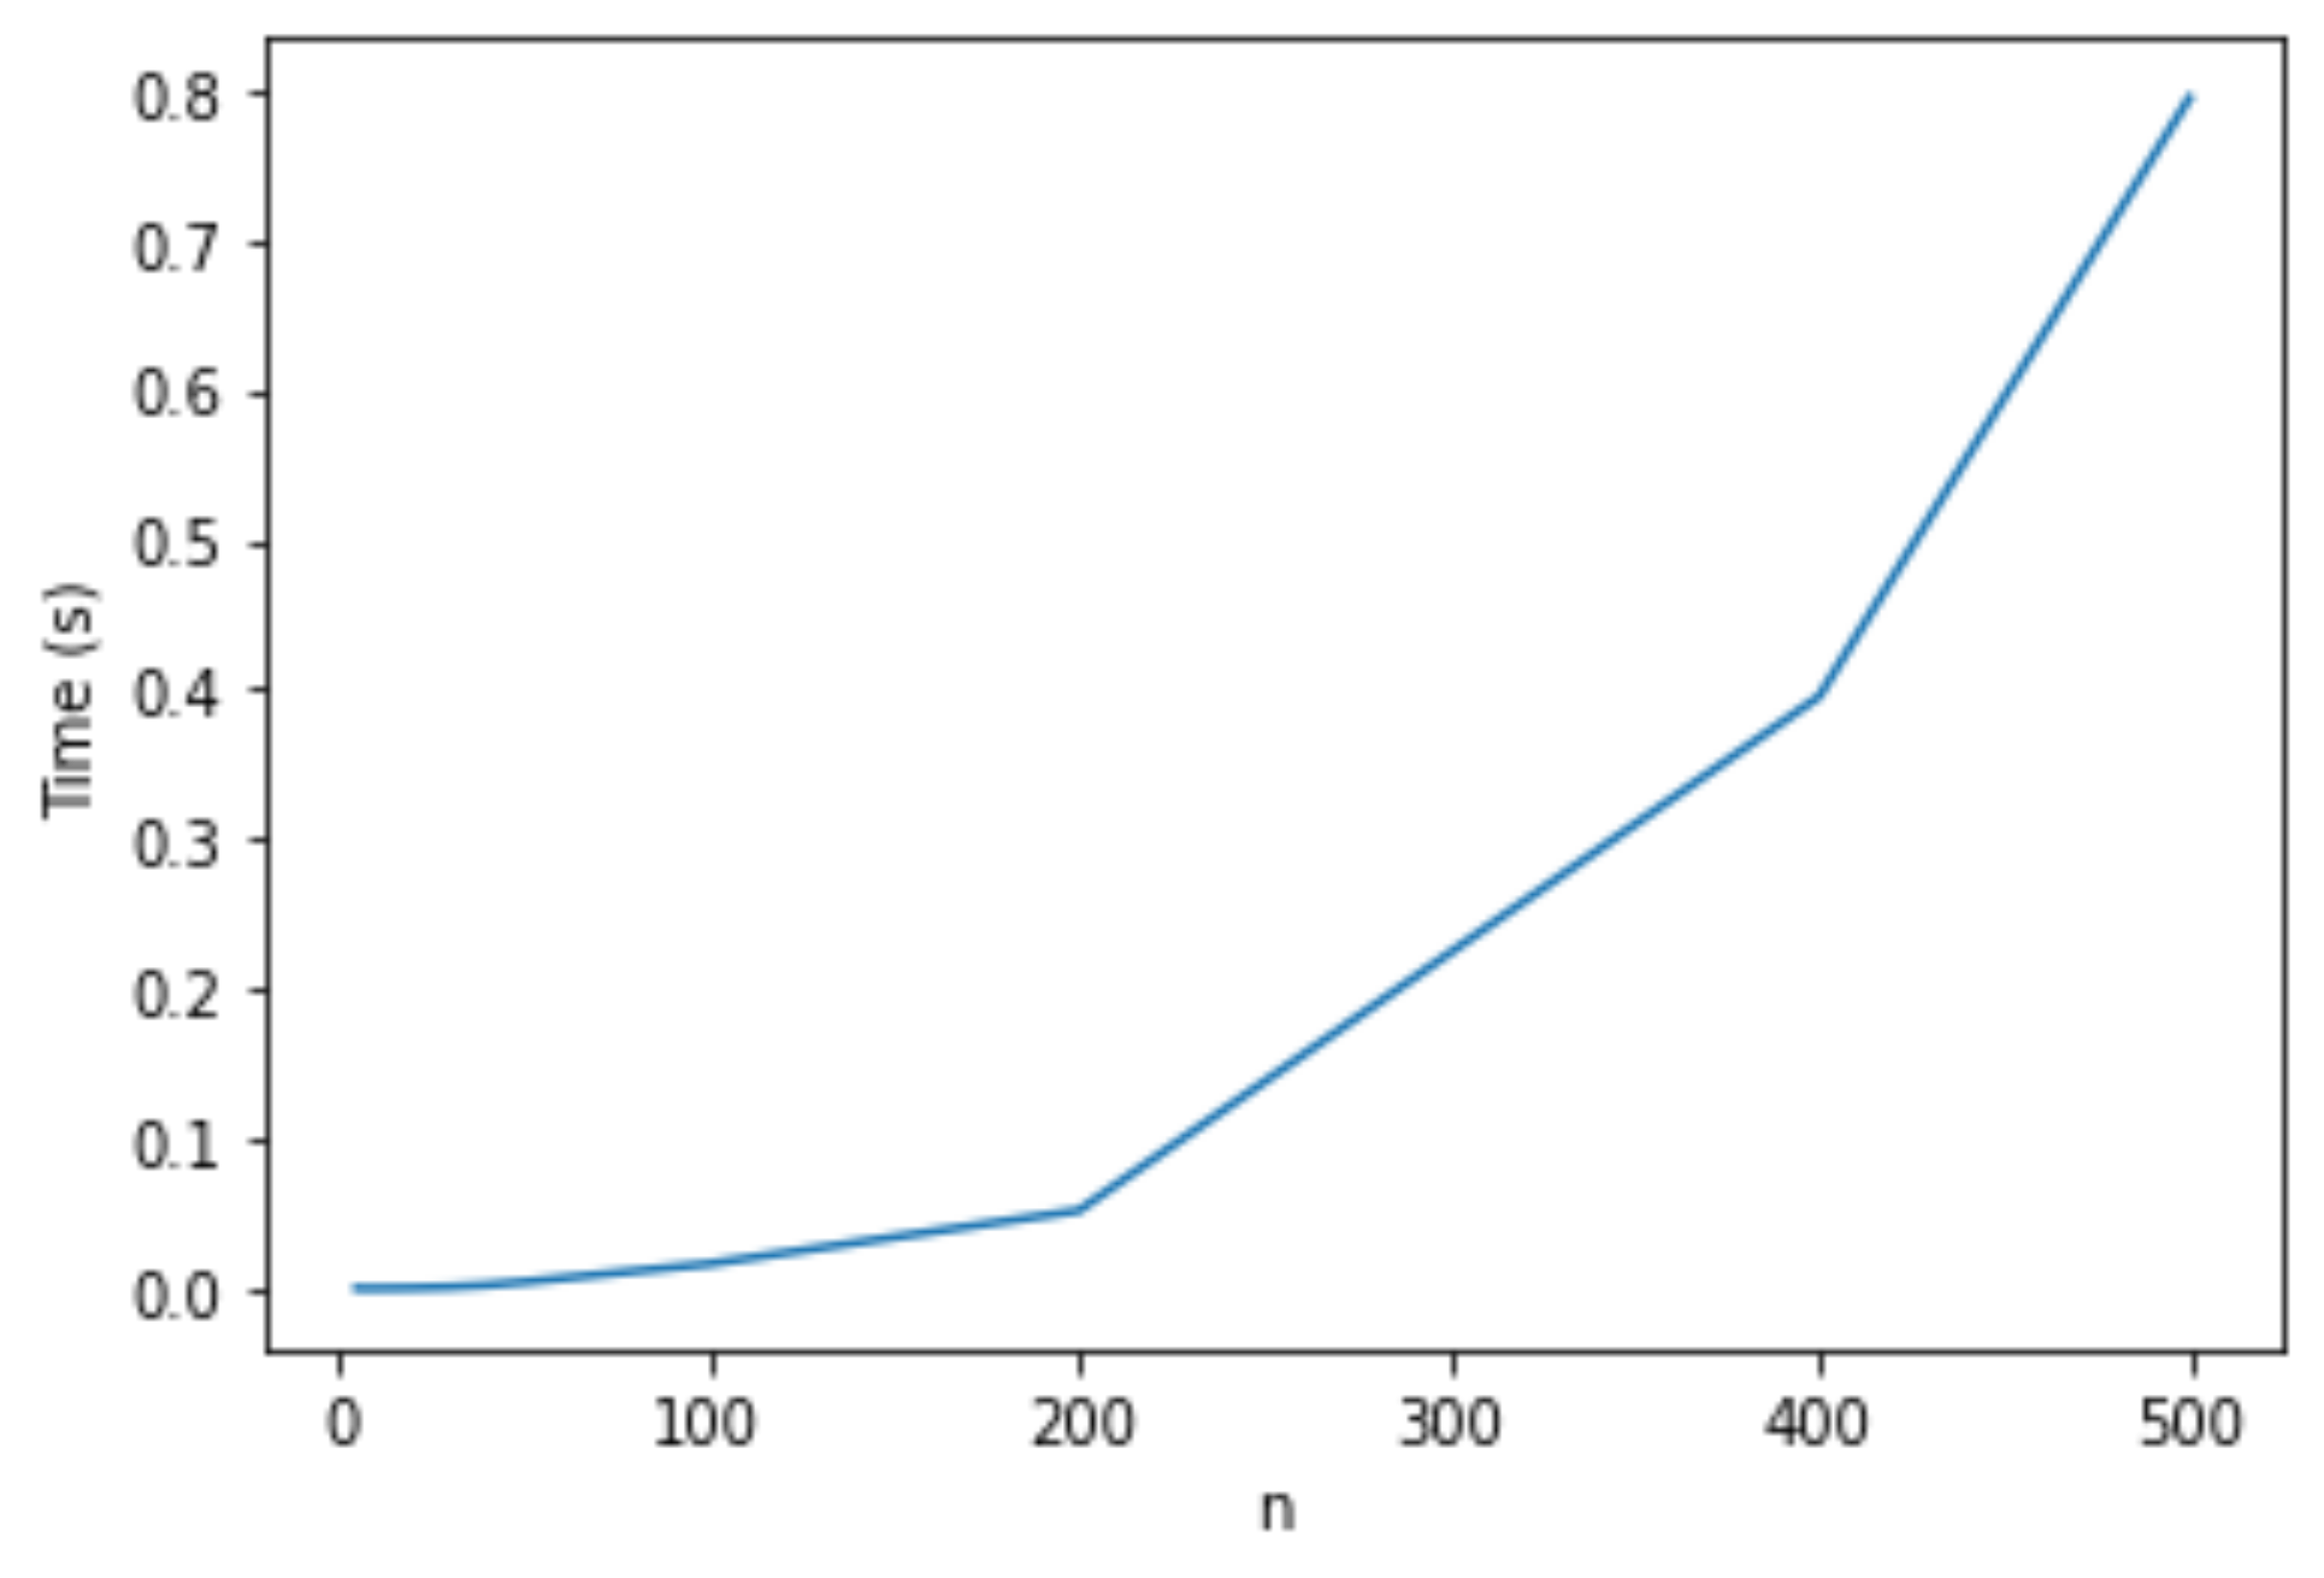
\includegraphics[width=1\linewidth]{figures/tempoTri.png}
					\end{center}
				\end{figure}
			\end{minipage}
			\hspace{0.1cm}
			\begin{minipage}{0.45 \linewidth}
				
				\begin{figure}[H]
					\begin{center}
						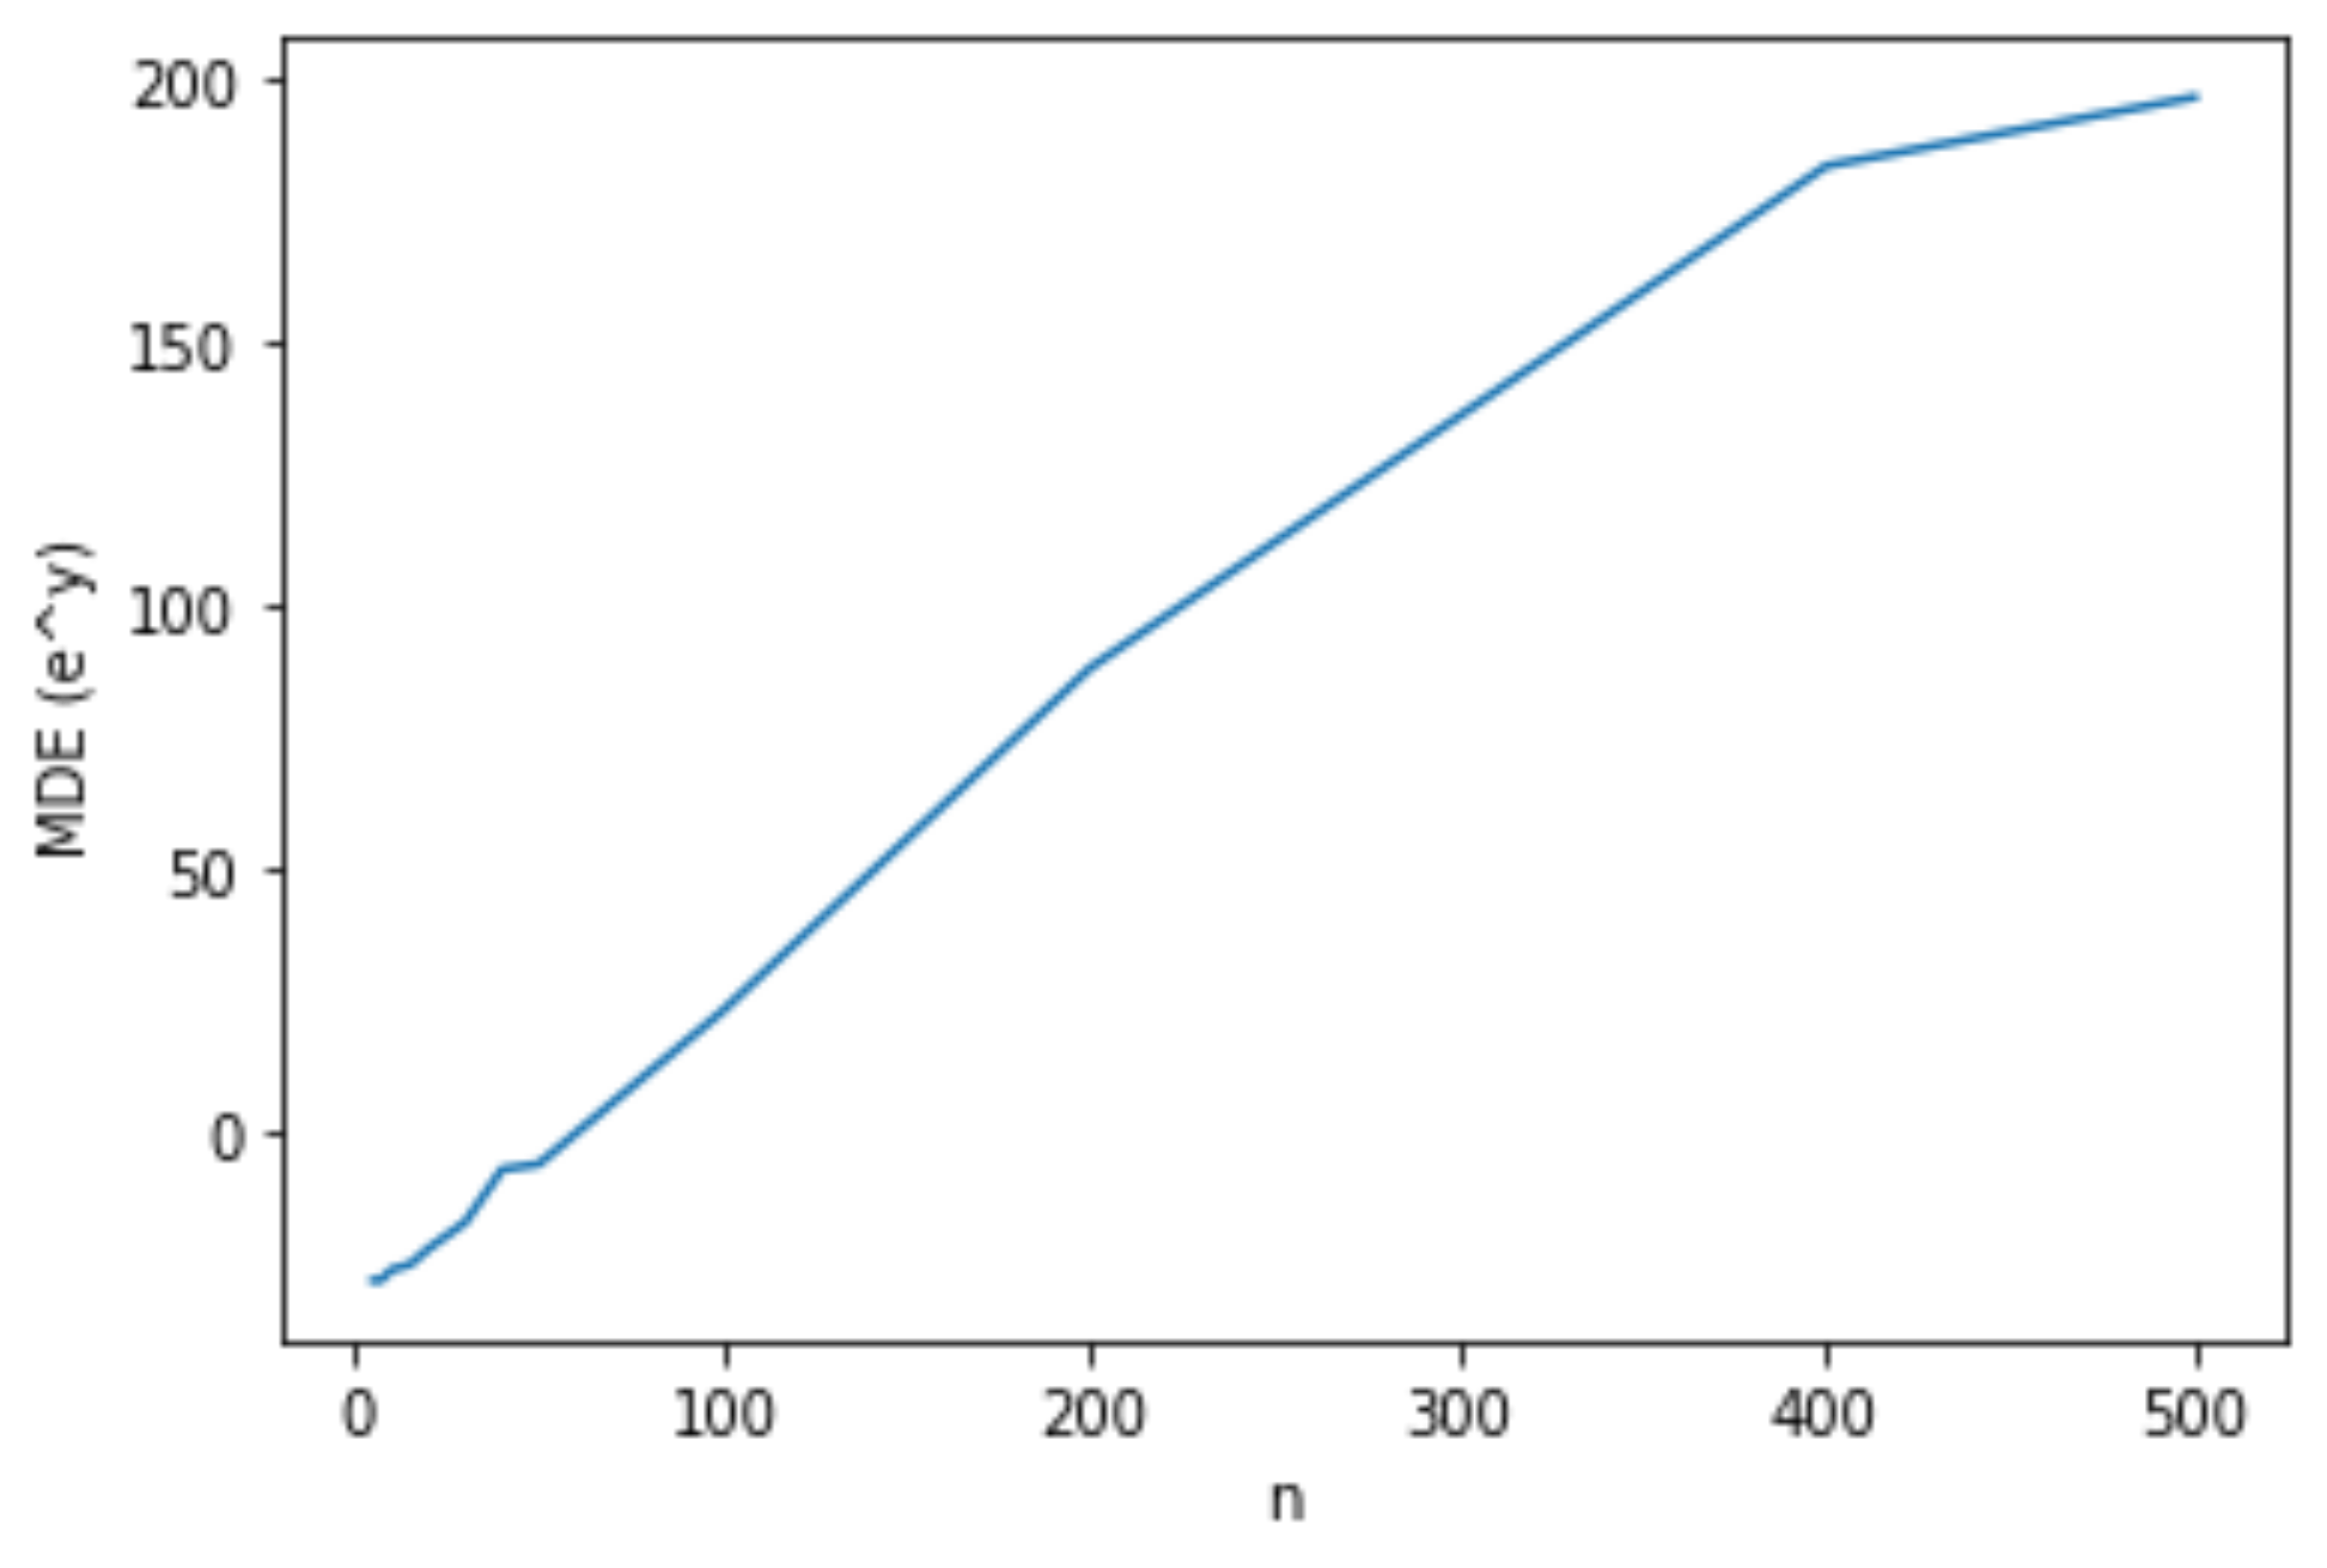
\includegraphics[width=1\linewidth]{figures/mdeTri.png}
					\end{center}
				\end{figure}
			\end{minipage}
		\end{center}
		\caption{A esquerda, o tempo de processo e, a direita, a ordem de grandeza associada ao MDE das soluções.}
		\label{fig:tri}
	\end{figure}
	
	Perceba o comportamento mostrado na Figura~\ref{fig:tri}. Teve-se que fazer uma linearização no gráfico que representa o MDE da solução, pois este cresceu exponencialmente e foi para a ordem de $10^{200}$ em 500 vértices. Esse comportamento se deu por conta dos erros acumulados entre as iterações.
	\\
	
	Uma proposta pensada para contornar essa situação infeliz foi alterar o valor de $\mathcal{P}$, deixando o menor, obrigando o algorítimo a calcular realizações utilizando vértices iniciais. Porém, isso implicaria em um grafo não completo, o que não condiz definição do Algorítimo~\ref{alg:realizacaoIterativa}.
	
	Outra solução proposta fora de utilizar sempre os primeiros vértices no lugar dos antecessores mais próximos. Isso significaria utilizar sempre os vértices âncoras para realizar os demais, semelhante com o que é feito no sistema GPS. Com isso, tivemos os resultados satisfatórios apresentados pela Figura~\ref{fig:triPri}. Perceba que mesmo com 500 vértices ainda obteve-se resultados com $MDE$ na ordem de $10^{-20}$.
	
	\begin{figure}[H]
		\begin{center}
			\begin{minipage}{0.45 \linewidth}
				\begin{figure}[H]
					\begin{center}
						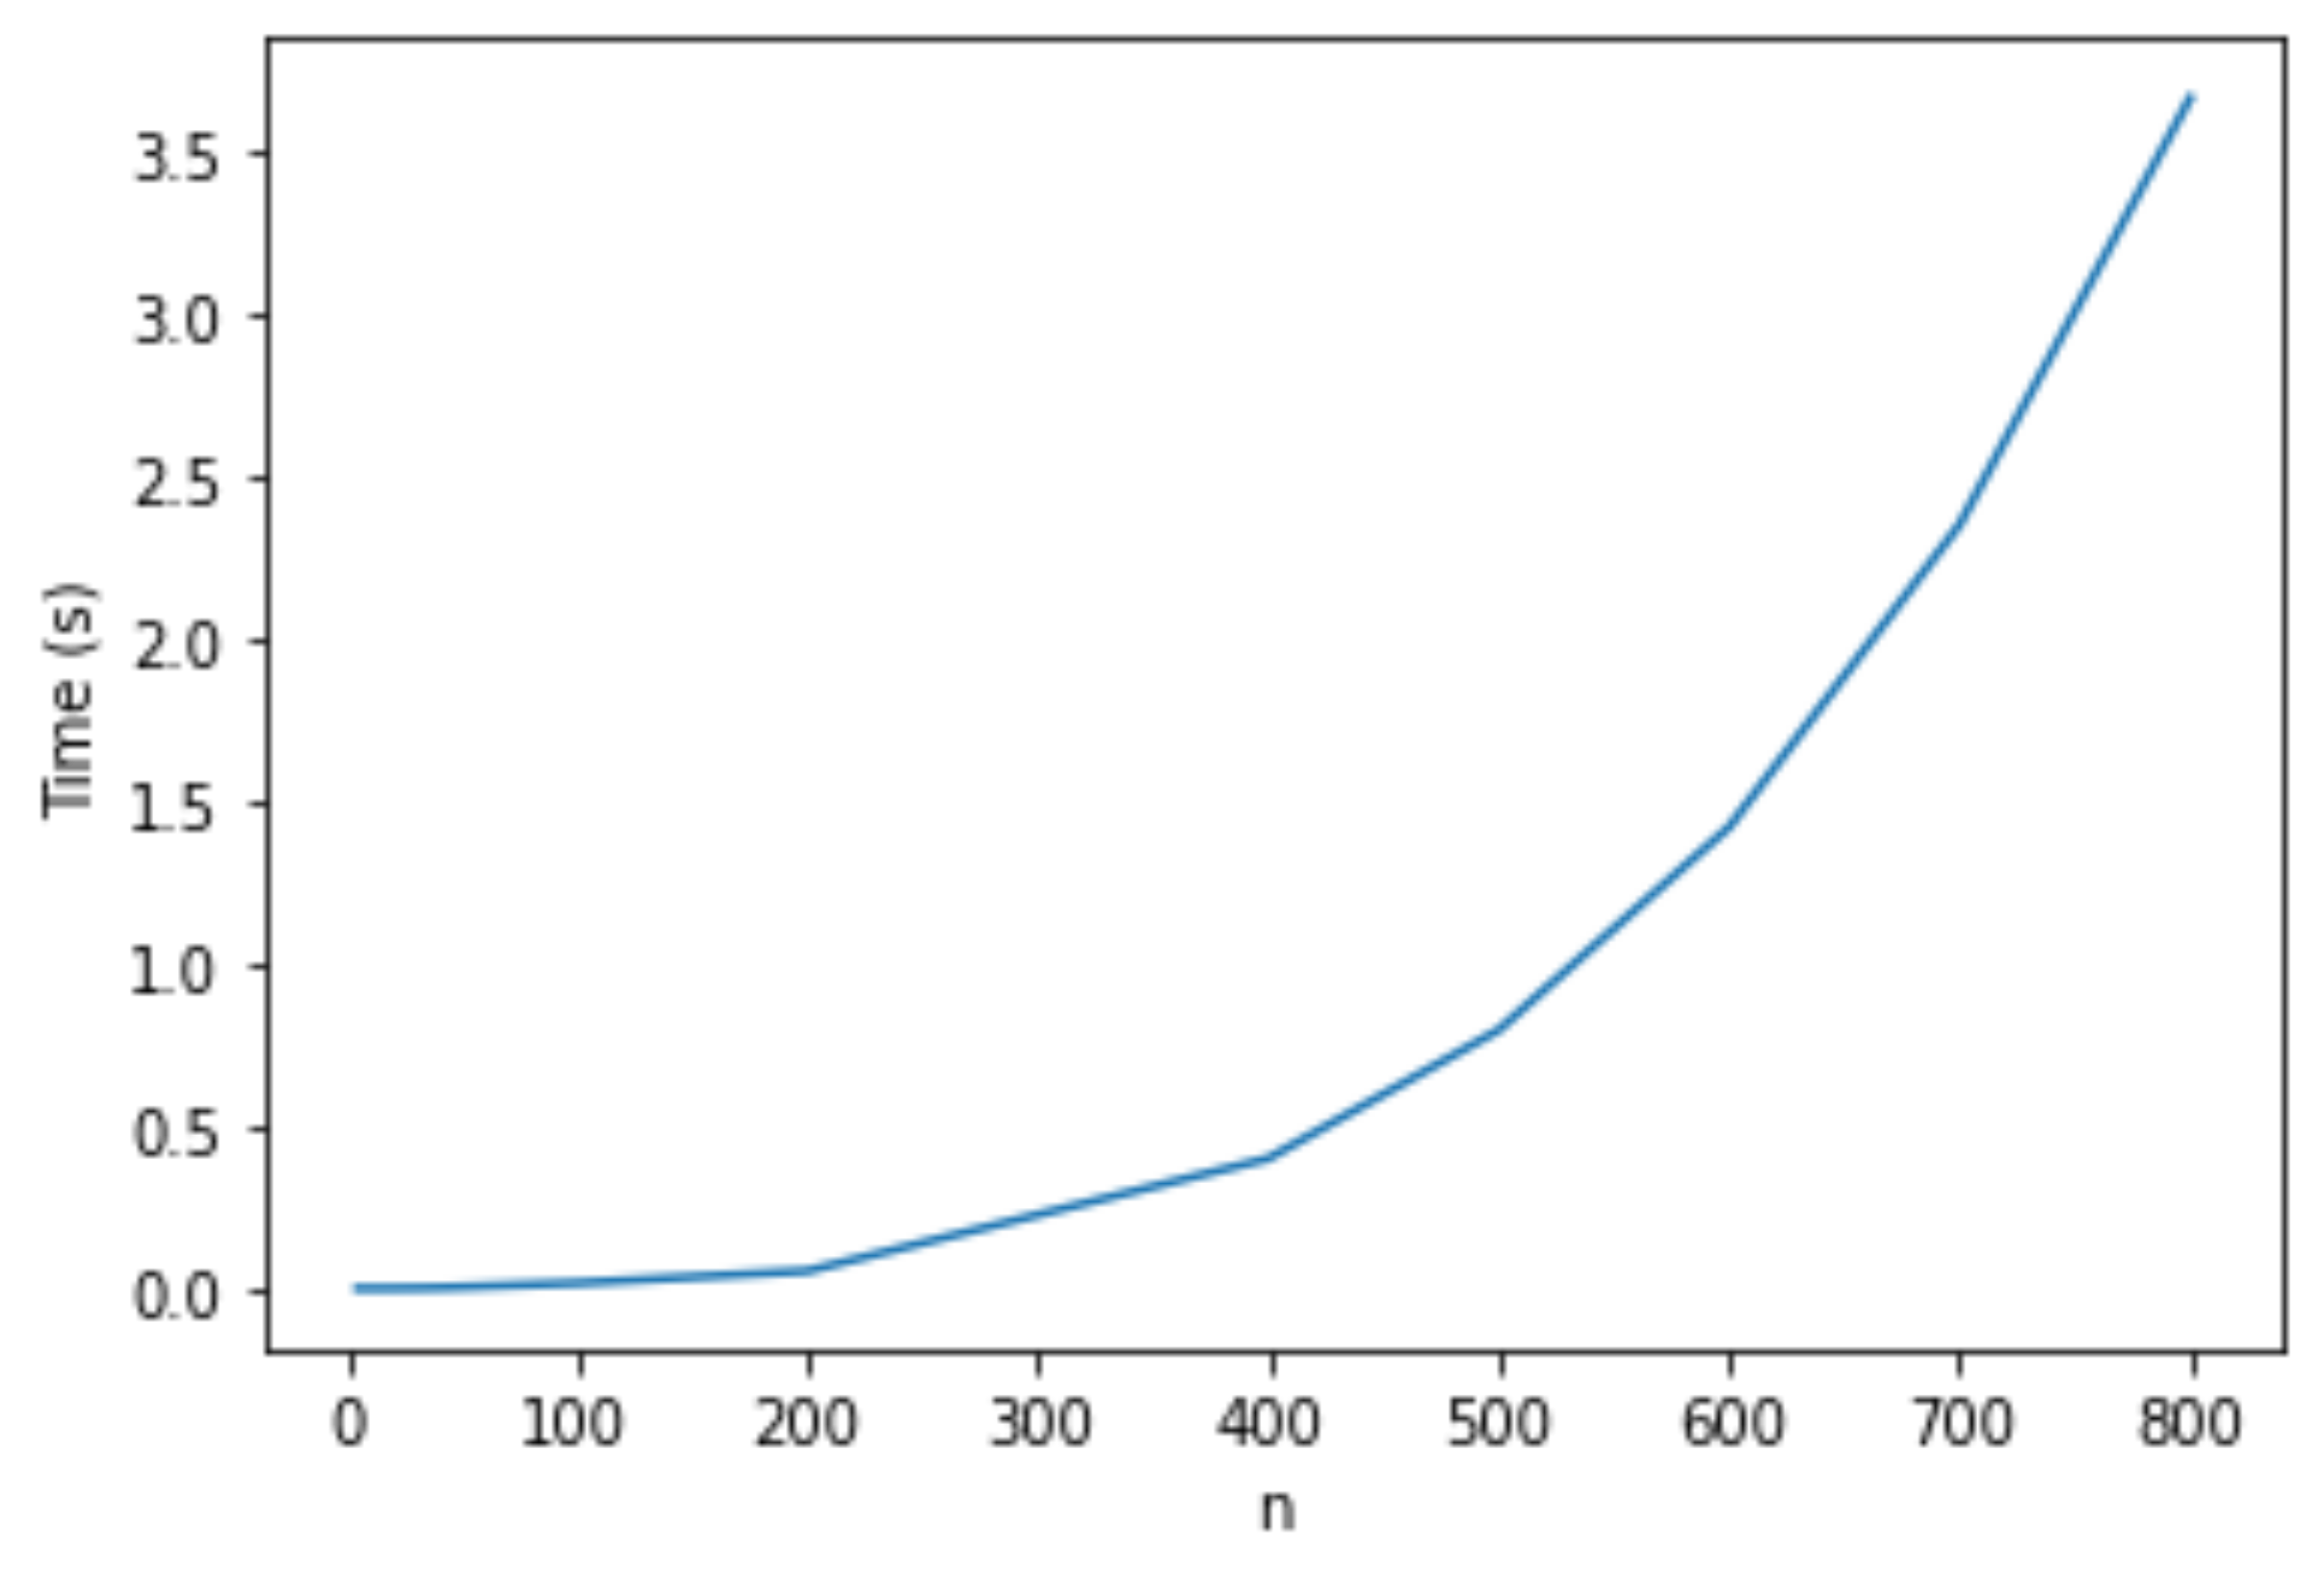
\includegraphics[width=1\linewidth]{figures/tempoTriPri.png}
					\end{center}
				\end{figure}
			\end{minipage}
			\hspace{0.1cm}
			\begin{minipage}{0.45 \linewidth}
				
				\begin{figure}[H]
					\begin{center}
						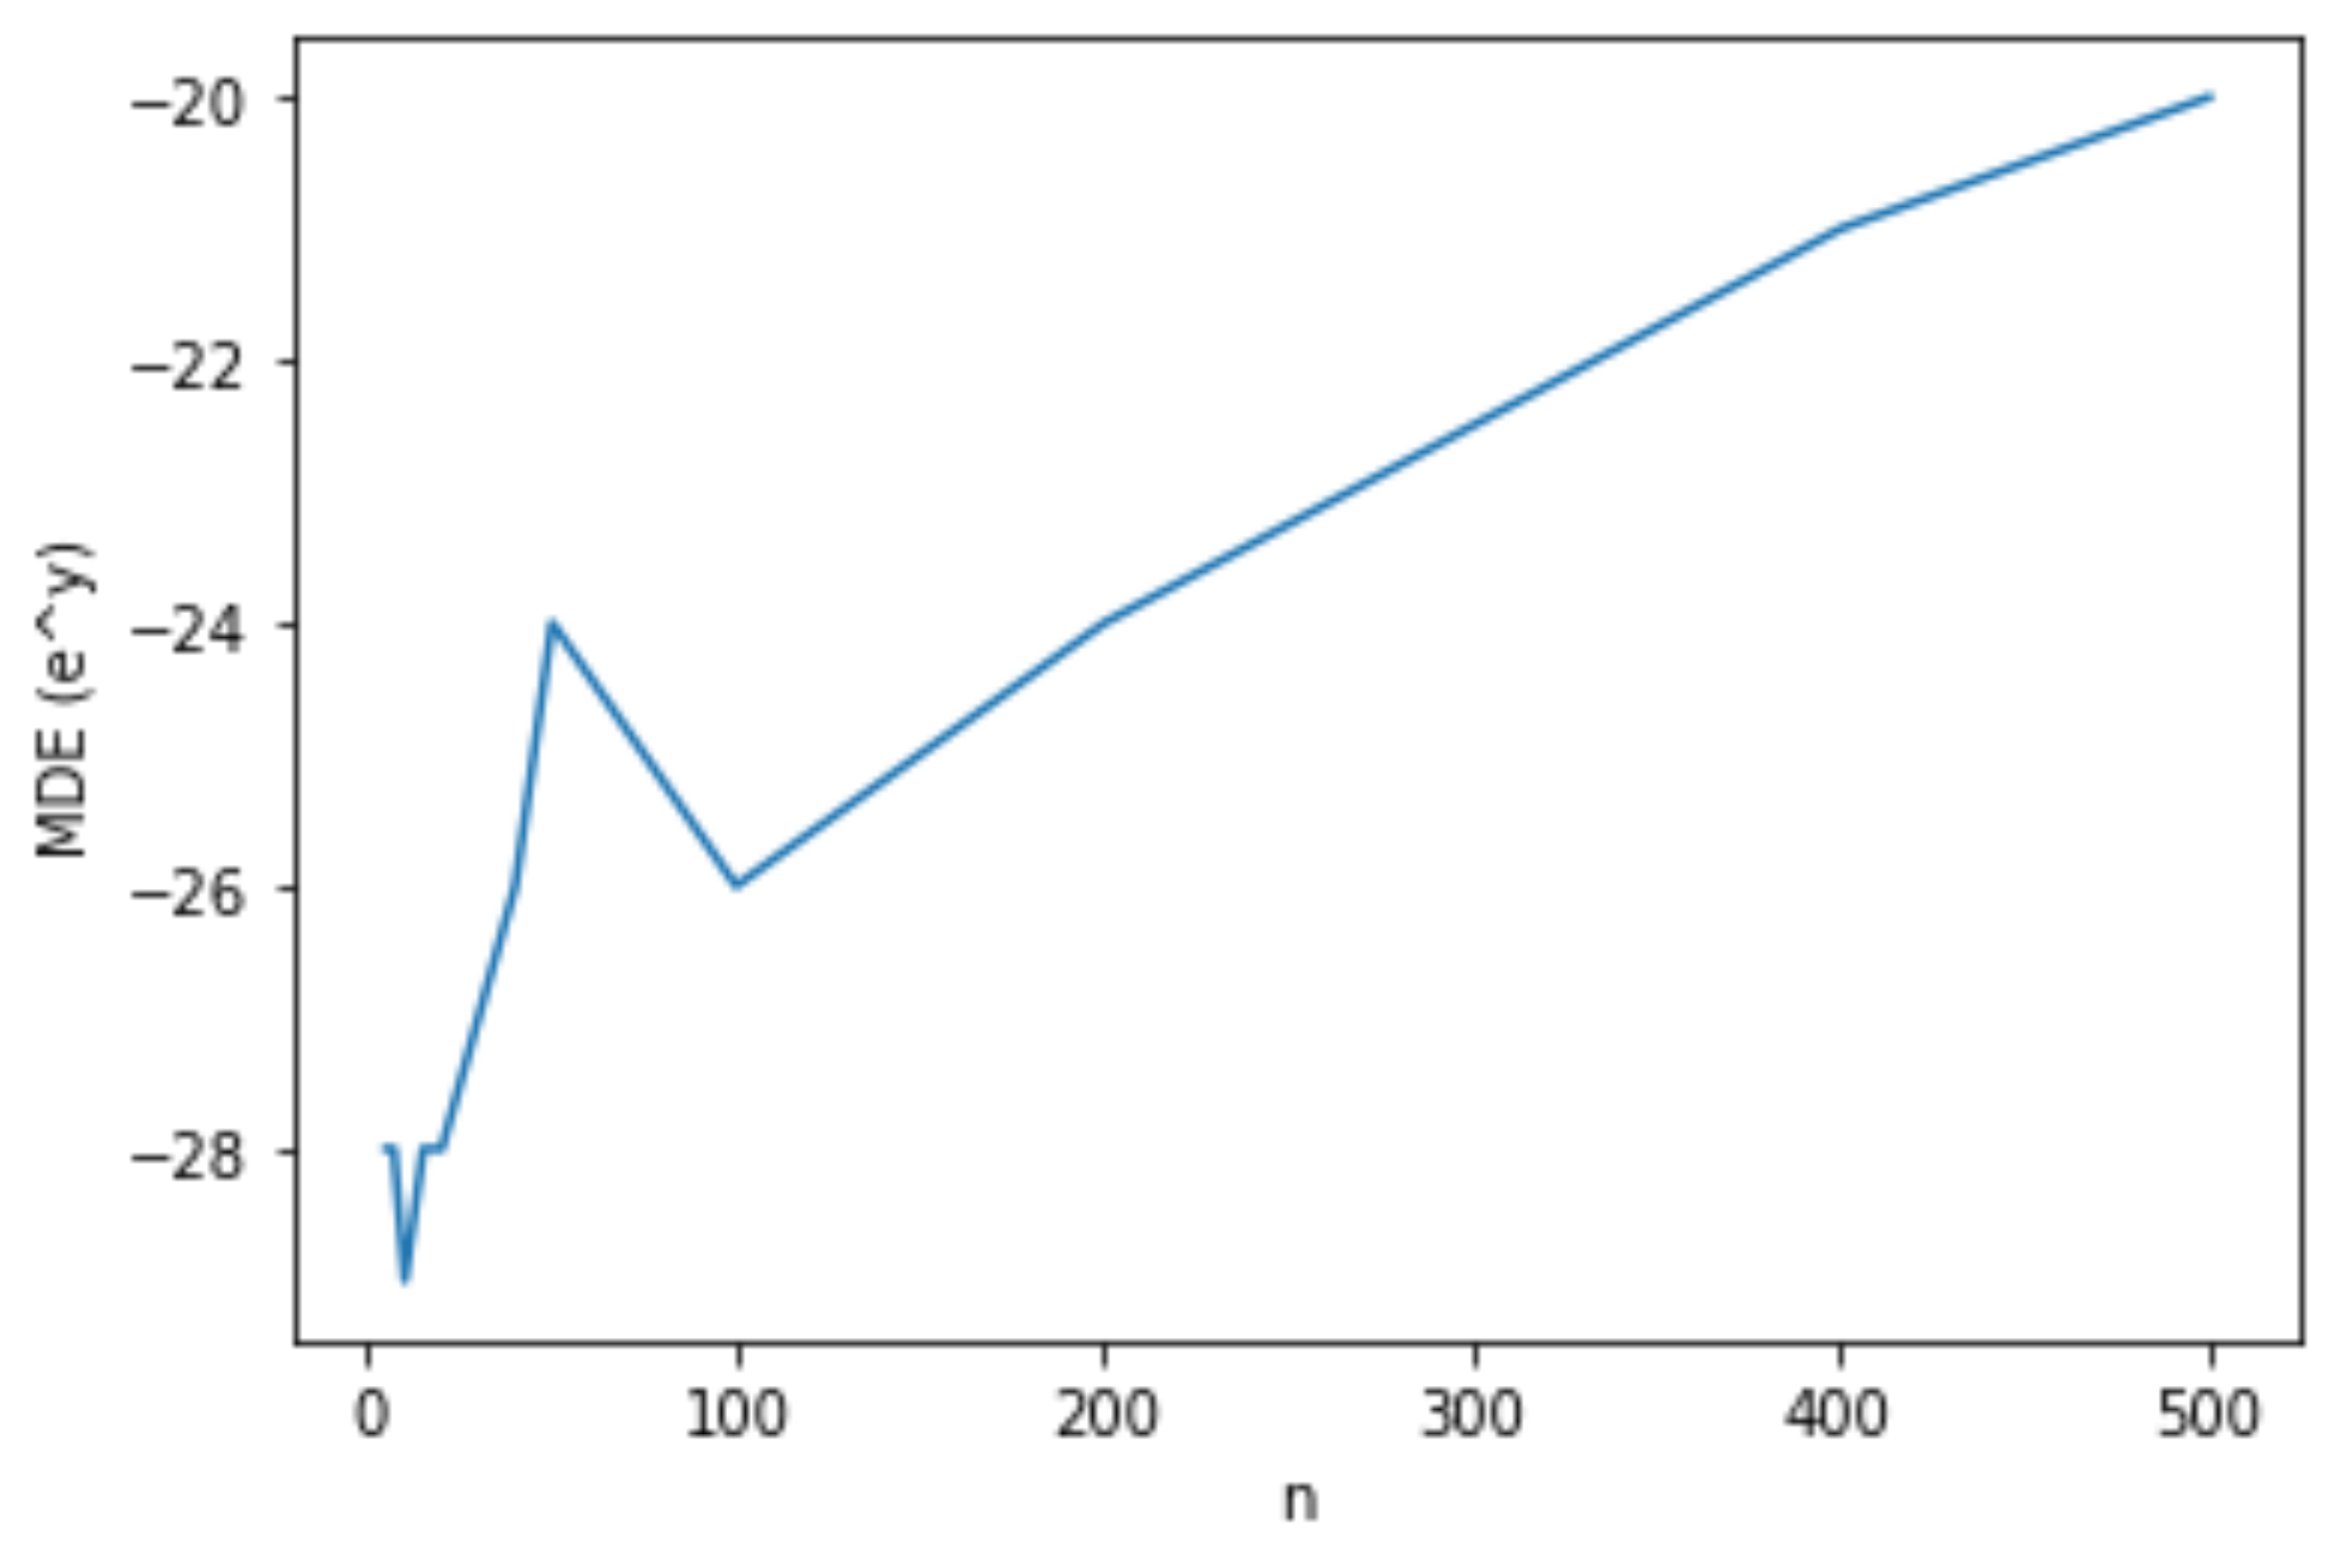
\includegraphics[width=1\linewidth]{figures/mdeTriPro.png}
					\end{center}
					\label{fig:mdeTri}
				\end{figure}
			\end{minipage}
		\end{center}
		\caption{A esquerda, o tempo de processo e, a direita, a ordem de grandeza associada ao MDE das soluções.}
		\label{fig:triPri}
	\end{figure}
	
	Também simulou-se o Algorítimo~\ref{alg:realizacaoTrilateration}, que teve um comportamento muito similar ao Algorítimo~\ref{alg:realizacaoIterativa}, como era de se esperar. Também usou-se instâncias $n$ variando em $\{5, 6, 7,10,15,20,30,40,50,100,200,400,500\}$. Porém, agora, com uma busca inteligente por vértices adjacentes, pode-se variar $\mathcal{P}$ afim de analisar diferentes geometrias para o problema, como apresenta-se a seguir.
	
	\subsubsection*{Instâncias com 70\% de arestas}
	
	\begin{figure}[H]
		\begin{center}
			\begin{minipage}{0.45 \linewidth}
				\begin{figure}[H]
					\begin{center}
						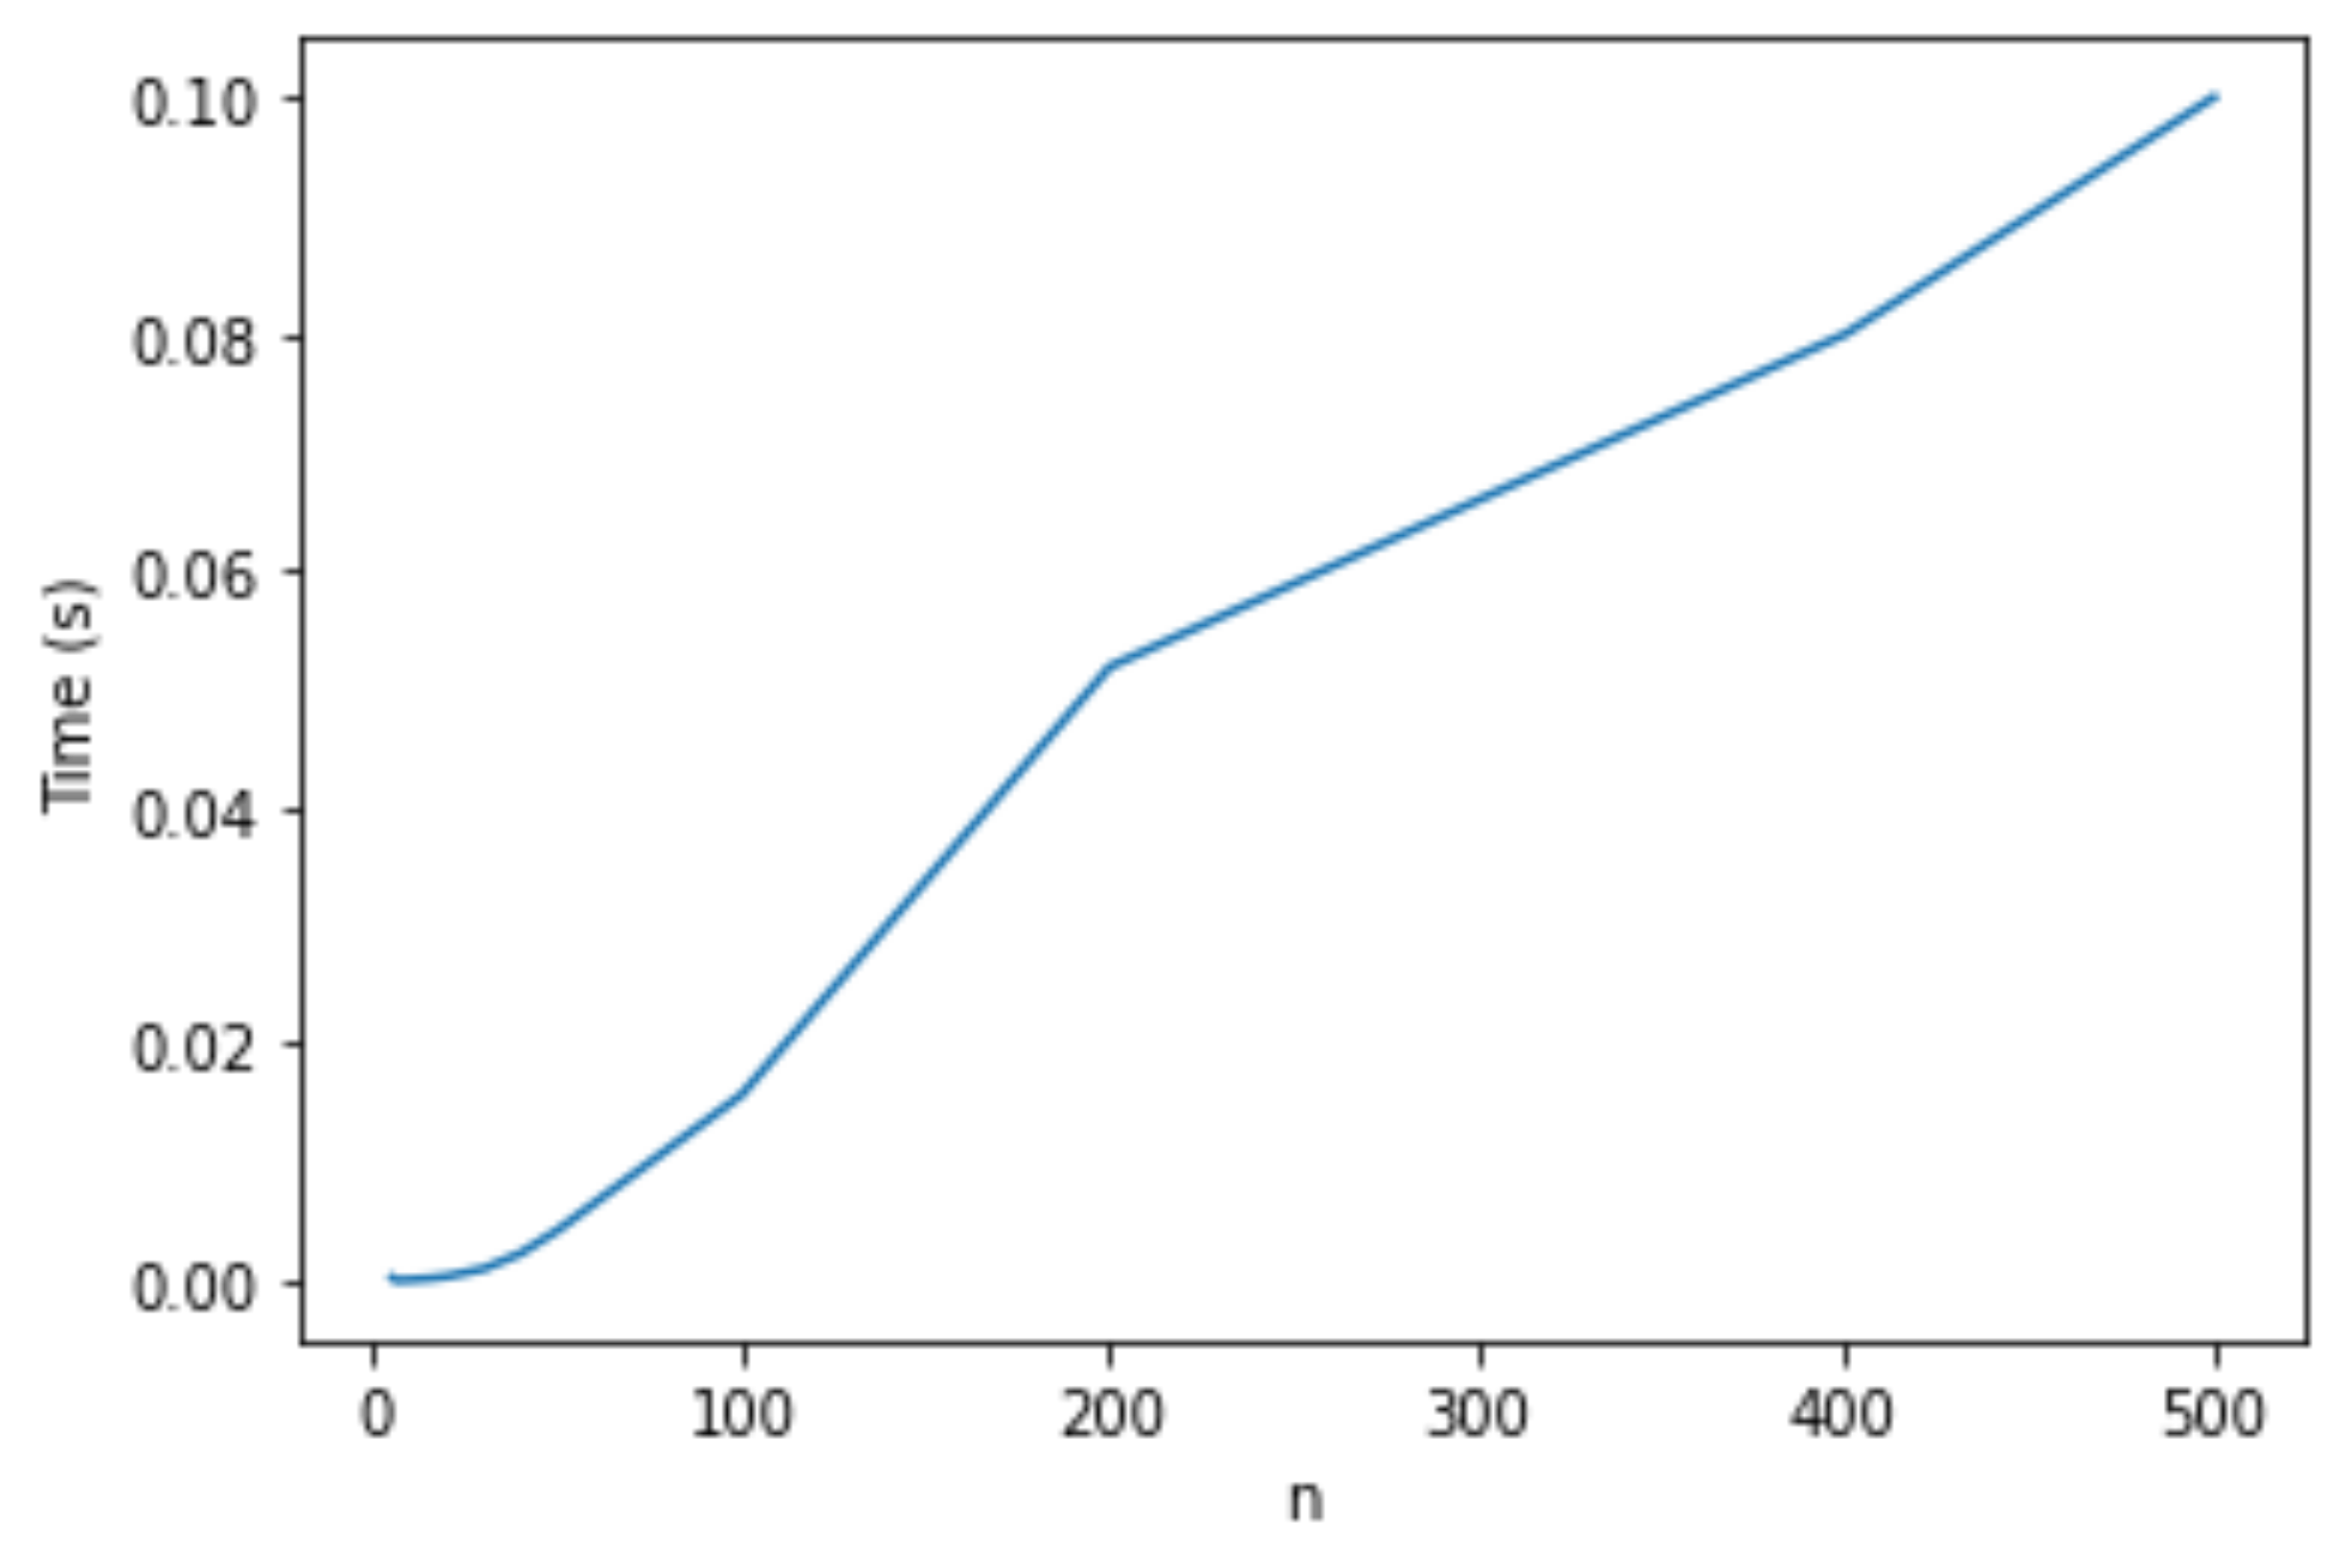
\includegraphics[width=1\linewidth]{figures/timeTriPro1.png}
					\end{center}
				\end{figure}
			\end{minipage}
			\hspace{0.1cm}
			\begin{minipage}{0.45 \linewidth}
				
				\begin{figure}[H]
					\begin{center}
						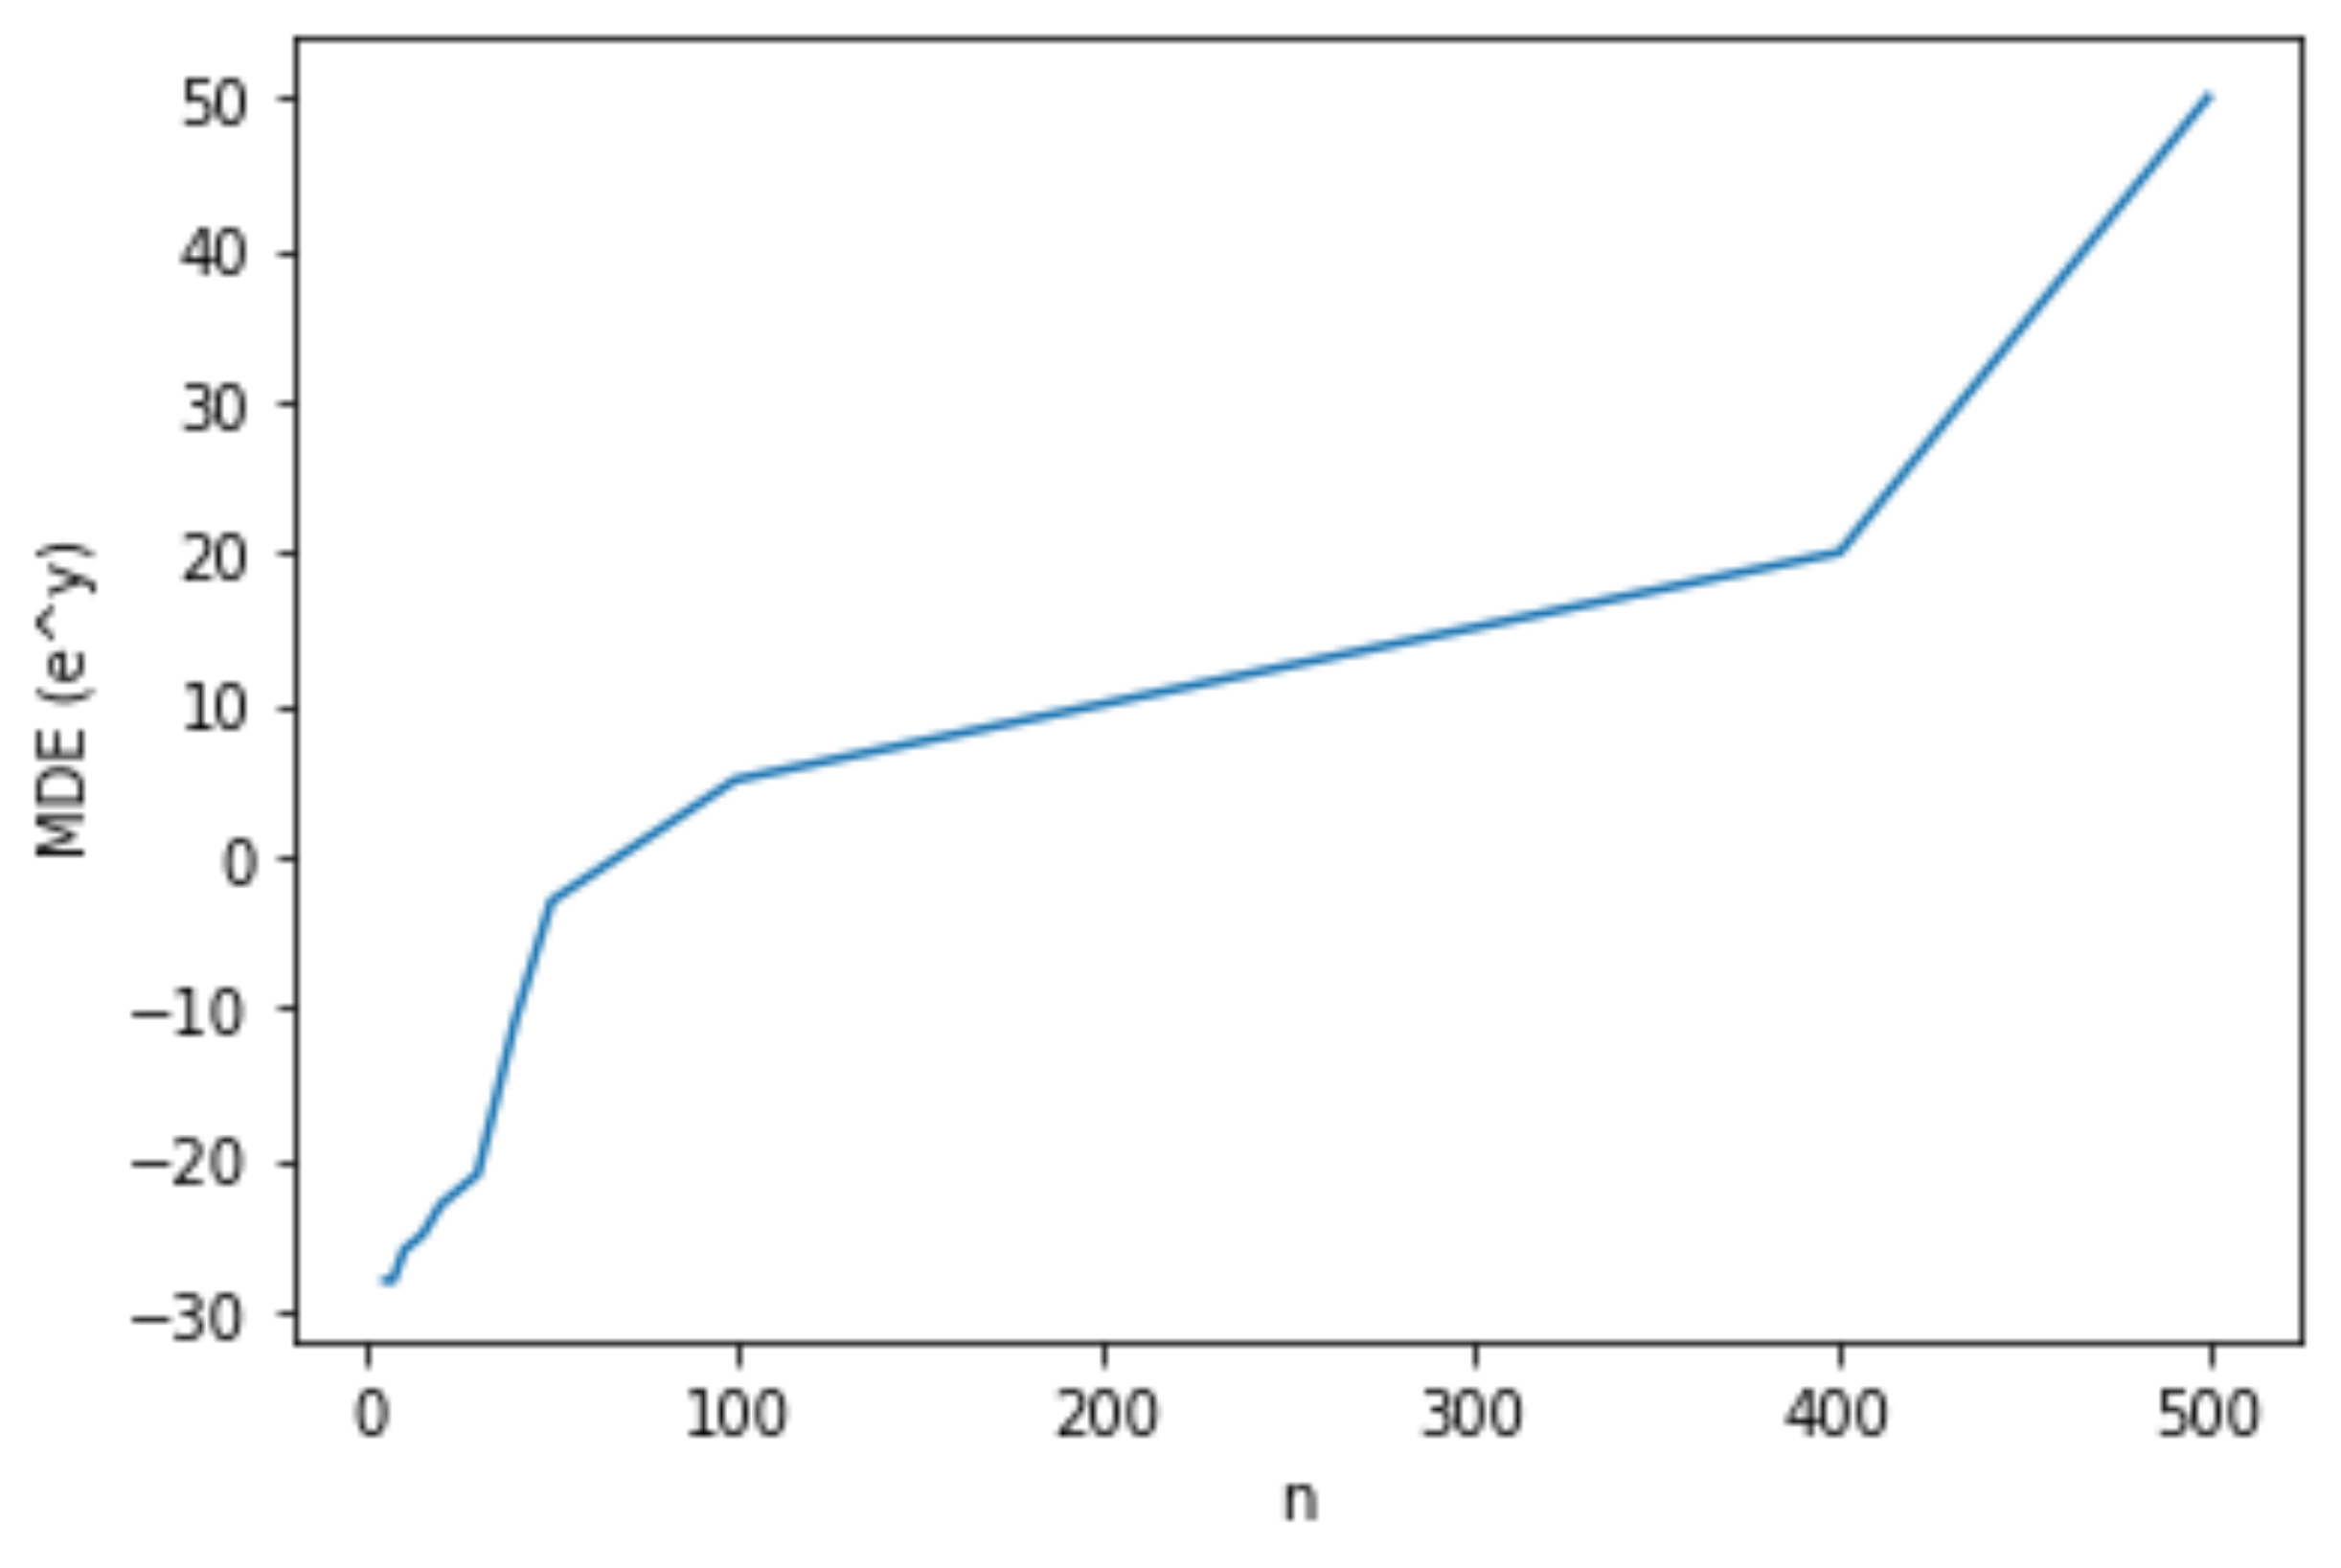
\includegraphics[width=1\linewidth]{figures/mdeTriPro1.png}
					\end{center}
					\label{fig:mdeTri}
				\end{figure}
			\end{minipage}
		\end{center}
		\caption{A esquerda, o tempo de processo e, a direita, a ordem de grandeza associada ao MDE das soluções. Utilizou-se $\mathcal{P} = 0.7$.}
		\label{fig:triPri4}
	\end{figure}
	
	\subsubsection*{Instâncias com 5\% de arestas}
	
	\begin{figure}[H]
		\begin{center}
			\begin{minipage}{0.45 \linewidth}
				\begin{figure}[H]
					\begin{center}
						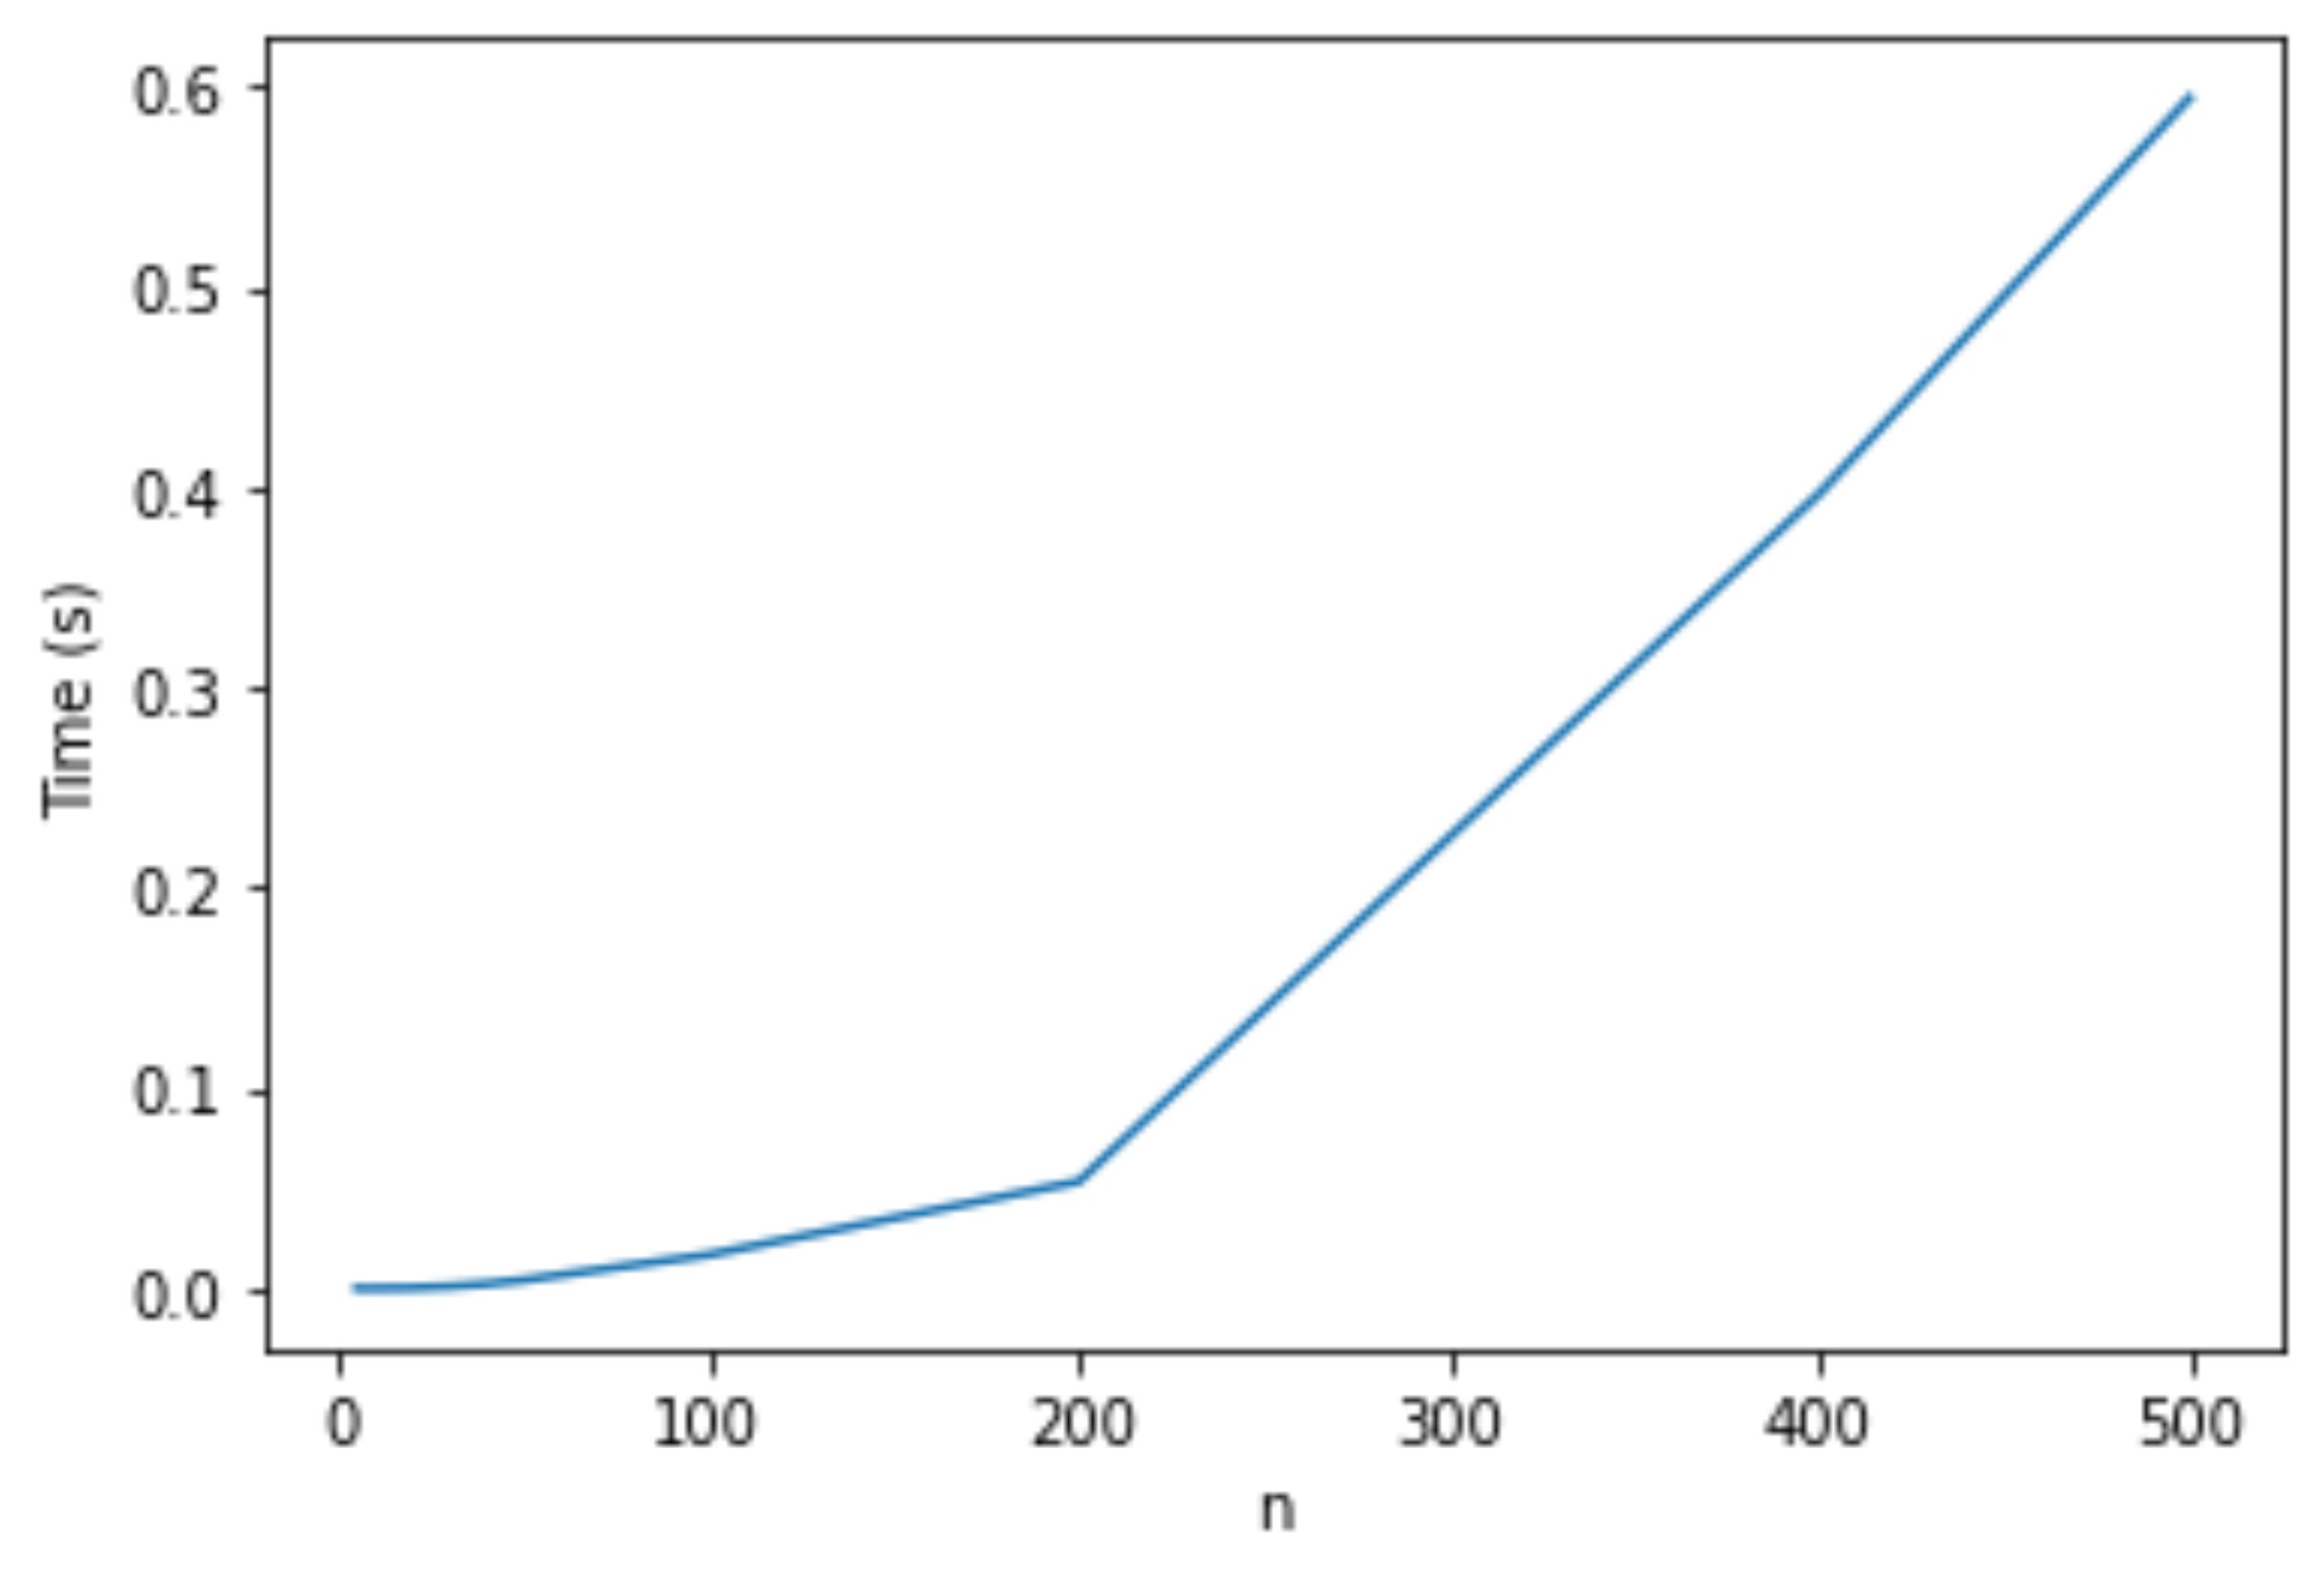
\includegraphics[width=1\linewidth]{figures/timePro2.png}
					\end{center}
				\end{figure}
			\end{minipage}
			\hspace{0.1cm}
			\begin{minipage}{0.45 \linewidth}
				
				\begin{figure}[H]
					\begin{center}
						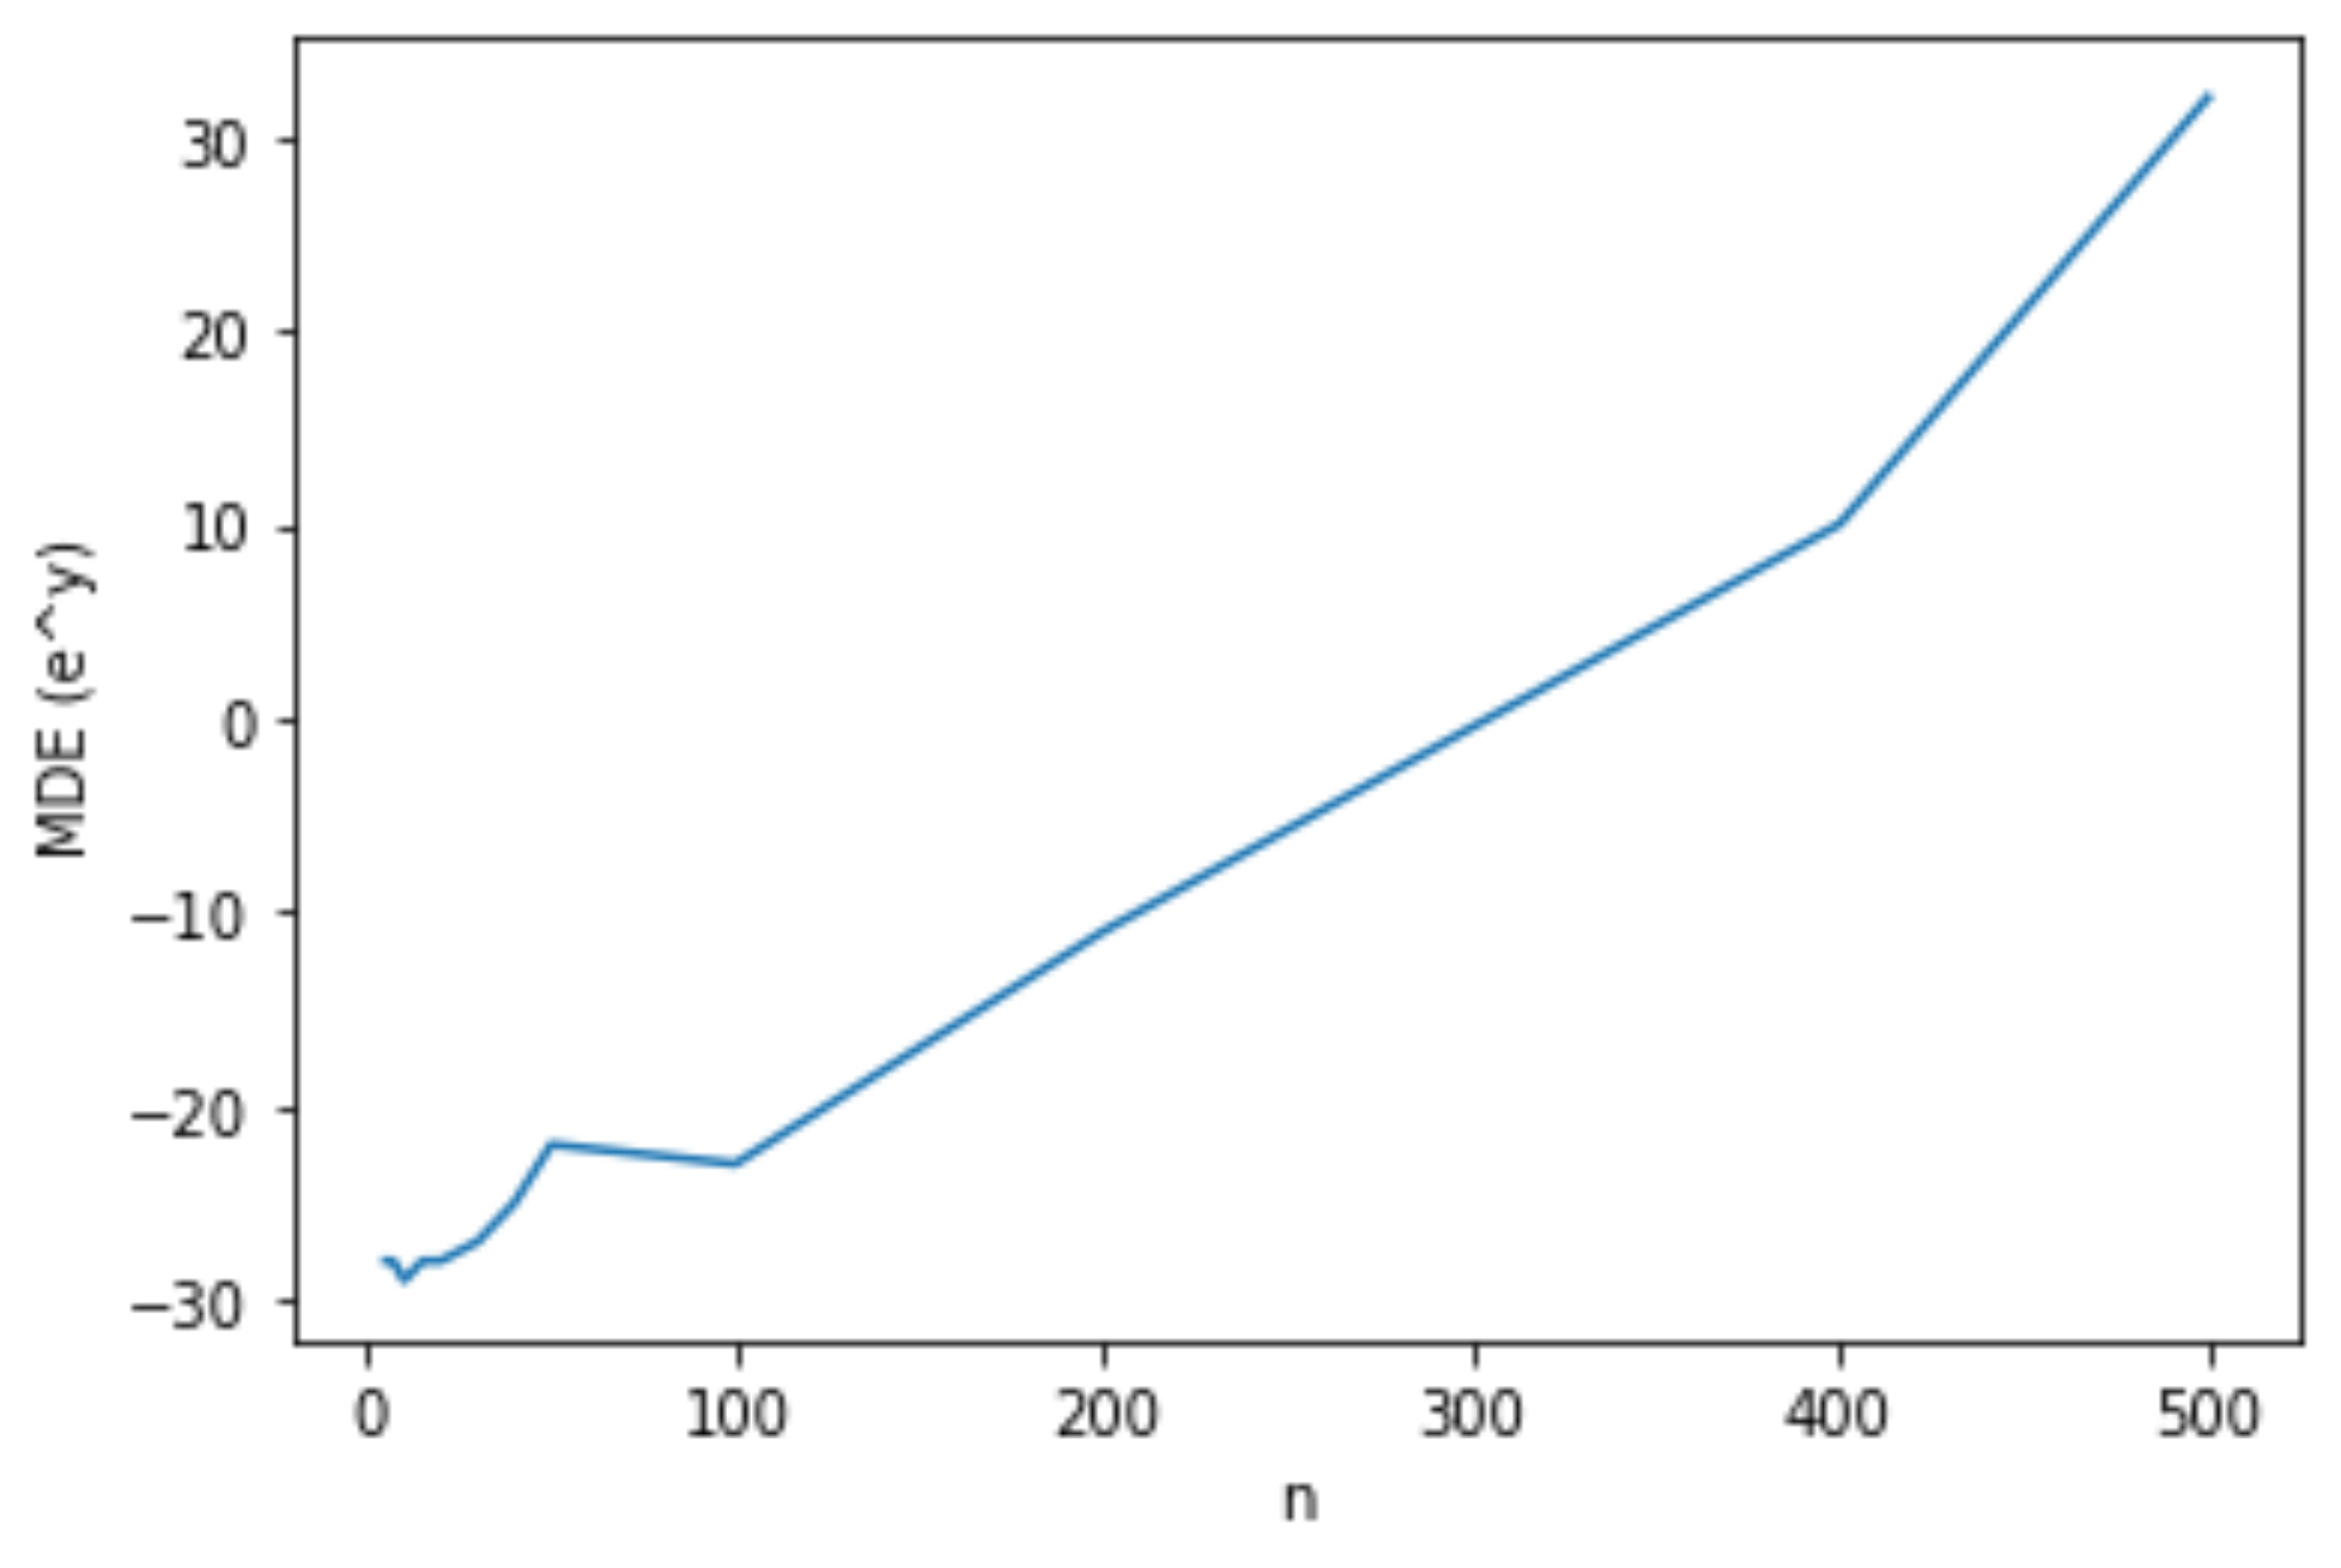
\includegraphics[width=1\linewidth]{figures/mdeTriPro2.png}
					\end{center}
					\label{fig:mdeTri}
				\end{figure}
			\end{minipage}
		\end{center}
		\caption{A esquerda, o tempo de processo e, a direita, a ordem de grandeza associada ao MDE das soluções. Utilizou-se $\mathcal{P} = 0.05$.}
		\label{fig:triPri3}
	\end{figure}
	
	Como esperado, é perceptível uma grande melhora na MDE das soluções conforme se diminui o valor de $\mathcal{P}$. 
	
	Também deve-se perceber que o tempo não obedeceu um padrão perfeito. Podemos relacionar esse fato com a aleatoriedade das instâncias, como pode-se notar que o Algoritmo~\ref{alg:realizacaoTrilateration} teve maios volatilidade no padrão temporal. Mesmo assim, há um consenso. As soluções mostradas nas Figuras~\ref{fig:triPri} e~\ref{fig:triPri3}, por exemplo, demonstram claramente um padrão polinomial, indo de encontro com o que foi apresentado na seção~\ref{sec:oi}.
	
	\newpage
	\section{Considerações Finais}
	Com isso, concluí-se o estudo sobre a Geometria de Distâncias aplicada ao problema de localização de sensores, tal qual teve como resultado um algorítimo que garante encontrar a solução do problema (se houver). .
	\\
	
	Nos cabe, nesse momento, voltarmos atenção às propostas levantadas internamente no início do projeto e verificar se elas foram cumpridas. Seguem o conjunto de objetivos específicos desse projeto, munidos de breve conclusão:
	
	\begin{enumerate}
		
		\item Estudar formas viáveis (pelos vieses energético, de construção e precisão da medida) para obtenção das distâncias entre os elementos do sistema físico:
		
		Fortemente embasado em \cite{savvides2001dynamic} e \cite{sensorsForMobileRobots}, faz-se uma apresentação sobre esses conceitos na Seção~\ref{sec:sensores}. 
		
		\item Estudar as possíveis distribuições dos Robôs Móveis em um sistema genérico, visando verificar quais conjuntos de dados possam ser garantidos como entradas para a construção do problema:
		
		Além de estudar distribuições genéricas, como em \cite{eren2004rigidity}, desenvolve-se na Seção~\ref{sec:disc} o Algorítimo~\ref{alg:instancia}, que cria instâncias aleatórias com diferentes densidades de ligações.
		
		\item Verificar a solução do Discretizable Order Problem \cite{carlileGDandAplications} aplicado ao problema proposto e estudar o ordenamento de vértices que se adeque aos objetivos do trabalho:
		
		Durante o desenvolvimento da Seção~\ref{sec:GD}, percebeu-se que uma ordem de discretização não seria necessária, visto que a definição do problema necessita de uma única solução \cite{libertiEDG}. Por conta disso, definiu-se a ordem de $K$-lateração, que garante a unicidade de solução.
		
		\item Caso consiga-se uma boa ordenação para os vértices, verificar a aplicação do algorítimo Branch-And-Prune \cite{carlile:BP} para a solução do problema proposto. Se não for possível, estudar outros algorítimos que possam solucionar o problema:
		
		Visto que o problema não era discreto, não fora possível aplicar o algorítimo Branch-And-Prune. Ao invés disso, se propôs o Algorítimo~\ref{alg:realizacaoTrilateration}, que utiliza a trilateração como núcleo e garante no máximo uma solução.
		
		\item Estudar a complexidade computacional do algorítimo proposto aplicado as possíveis distribuições:
		
		Isso foi feito no fim das Seções~\ref{sec:GD} e~\ref{sec:disc}, onde verificou-se que o algorítimo pode ser resolvido em tempo polinomial. Também mostrou-se um estudo sobre diferentes visões da geometria do problema afim de minimizar os erros associados. 
		
		\item Simular computacionalmente o algoritmo para solução do problema com instâncias artificialmente geradas, dominando cada passo utilizado:
		
		Simulações apresentadas, de forma satisfatória, na Seção~\ref{sec:disc}.
		
		\item Aplicar o algoritmo estudado em estruturas de pequena escala, como instâncias reais do problema:
		
		Não fora possível cumprir este último objetivo. Infelizmente, a manufatura de robôs móveis usando sensores de distância se demonstrou excessivamente custosa \cite{savvides2001dynamic, sensorsForMobileRobots}.
		
		Vale lembrar, porém, que a utilização de instâncias artificiais genéricas se mostrou de grande importância. Pode-se averiguar e discutir sobre diferentes geometrias, mesmo sem a prototipação de fato.
		
	\end{enumerate}
	
	Como experiências futuras, deseja-se estudar mais sobre a obtenção e tratamento de dados de distâncias, visto que esses possuem erros de medida \cite{sensorsForMobileRobots} (não levados em consideração nesse trabalho). Alguns trabalhos relacionados à Geometria de Distâncias aplicada ao caso intervalar são mostrados em \cite{wsnlSemidefinitePrograming}. Há curiosidade em ver como medida MDE se comporta para uma quantidade grande de vértices associados a erros de medida.
	
	Também deseja-se fazer estudos sobre geometrias mínimas para o problema, como feito em \cite{wsnlFewAnchors}. Deseja-se verificar um conjunto de condições que restringem o movimento de um robô móvel afim de garantir que este ainda possa ser localizado.
	
	\newpage
	\phantomsection
	\addcontentsline{toc}{section}{Referências}
	
	\bibliographystyle{unsrt}
	\bibliography{references}
	
	\newpage
	\appendix
	\input{secGD/apendices.tex}

\end{document}

	
	\newpage
	
	 \documentclass[a4paper,12pt]{article}
\usepackage[a4paper,top=3cm,bottom=2cm,left=3cm,right=3cm,marginparwidth=1.75cm]{geometry}
\usepackage[brazil]{babel}
\usepackage[T1]{fontenc}
\usepackage[utf8]{inputenc}
\usepackage{amsmath}
\usepackage{MnSymbol}
\usepackage{wasysym}
\usepackage{hyperref}
\usepackage{color}
\definecolor{Blue}{rgb}{0,0,0.9}
\definecolor{Red}{rgb}{0.9,0,0}
\usepackage{esvect}
\usepackage{graphicx}
\usepackage{float}
\usepackage{indentfirst}
\usepackage{caption}
\usepackage{blkarray}
\newcommand\Mark[1]{\textsuperscript#1}
\usepackage{pgfplots}
\usepackage{amsfonts}
\usepackage[english, ruled, linesnumbered]{algorithm2e}
\usepackage{algorithmic}
\newtheorem{definicao}{Definição}[section]
\newtheorem{teorema}{Teorema}[section]

\title{Disposição de Robôs Móveis no espaço Euclidiano 3D: uma aplicação de Geometria de Distâncias}
\author{Guilherme Philippi\Mark{*}, orientado por Felipe Delfini Caetano Fidalgo\Mark{\dagger}\\Campus Blumenau\\Universidade Federal de Santa Catarina\\UFSC
	\\guilherme.philippi@grad.ufsc.br\Mark{*}, felipe.fidalgo@ufsc.br\Mark{\dagger}}
\begin{document}
	\begin{titlepage}
		\newcommand{\HRule}{\rule{\linewidth}{0.5mm}} % Defines a new command for the horizontal lines, change thickness here
		\center % Center everything on the page
		%----------------------------------------------------------------------------------------
		%	HEADING SECTIONS
		%----------------------------------------------------------------------------------------
		\begin{center}
			
\includegraphics[scale=0.22]{figures/logoufsc.jpg}
		\end{center}
		\vspace{1cm}
		
		\textsc{\LARGE \hspace{-0.17cm}Universidade Federal de Santa Catarina}\\[0.5cm] % Name of your university/college
		{\Large Centro de Blumenau \\ Departamento de Matemática}\\[1.5cm] % Major heading such as course name
		\textsc{\Large PIBIC \\ Relatório Final \vspace{1.5cm}  \\ }{\large Geometria de Distâncias e Álgebras Geométricas: novas perspectivas geométricas, computacionais e aplicações}\\[2.0cm] % Minor heading such as course title
		
		%\textsc{\LARGE Universidade Federal de Santa Catarina}\\[0.5cm] % Name of your university/college
		%{\Large Centro de Blumenau \\ Departamento de Matemática}\\[1.5cm] % Major heading such as course name
		%\textsc{\Large PIBIC \\ Programa Institucional de Bolsas de Iniciação Científica \vspace{1.5cm} \\ {\bf PROJETO DE PESQUISA}}\\[2.0cm] % Minor heading such as course title
		
		%----------------------------------------------------------------------------------------
		%	TITLE SECTION
		%----------------------------------------------------------------------------------------
		
		\HRule \\[0.4cm]
		{ \LARGE \bfseries \textbf{Disposição de Robôs Móveis no espaço Euclidiano 3D: uma aplicação de Geometria de Distâncias}} \\ [0.4cm] % Title of your document
		\HRule \\[2cm]
		
		%----------------------------------------------------------------------------------------
		%	AUTHOR SECTION
		%----------------------------------------------------------------------------------------
		
		\begin{minipage}{1\textwidth}
			\begin{center} \large
				Guilherme Philippi (g.philippi@grad.ufsc.br),
				\vspace{0.5cm}
				\\
				\underline{\textsc{Orientador:}} \vspace{0.2cm}
				Felipe Delfini Caetano Fidalgo (felipe.fidalgo@ufsc.br).
			\end{center}
		\end{minipage} \\[2cm]
		
		
		{\large \today} % Date, change the \today to a set date if you want to be precise
		
		
		\vfill % Fill the rest of the page with whitespace
		
	\end{titlepage}
	
	
	\newpage
	\vspace{-1cm}
	\tableofcontents
	\newpage
	
	\begin{center}
		\large
		\textbf{Abstract}
	\end{center}
	
	
	In this work, the Distance Geometry Problem Trilaterative applied to the sensor location problem was studied, as well as the necessary tools for its understanding, going from graph theory to the characteristics of systems involving mobile robotics. An overview of Geometry of Distances was presented, which enabled the correct definition of the problem and polynomial algorithms to solve it. The text ends with an analysis of computer simulations of the problem, using different geometries, as well as an algorithm to generate them.
	
	\textbf{Keywords:} TDGP, Distance Geometry, Mobile Robotics.
	
	
	\vspace{2cm}	
	\begin{center}
		\large
		\textbf{Resumo}
	\end{center}
	
	Neste trabalho, foram estudados o Trilaterativo Distance Geometry Problem aplicado ao problema de localização de sensores, bem como as ferramentas necessárias para sua compreensão, passando da teoria de grafos às características de sistemas envolvendo robótica móvel. Apresentou-se uma visão geral de Geometria de Distâncias que possibilitou a correta definição do problema e de algorítimos polinomiais para solucioná-lo. O texto se encerra com uma analise de simulações computacionais do problema, utilizando diferentes geometrias, bem como um algorítimo para gerá-las. 
	
	\textbf{Palavras-chave:} TDGP, Geometria de Distâncias, Robótica Móvel.
	
	
	\newpage
	\section{Introdução}
	
	Percebe-se uma tendencia de mercado em se adotar sistemas autônomos móveis para realizar funções que dependem de um grande número de maquinas, como o controle do estoque em um armazém, um sistema de entrega ou o cultivo e tratamento de grandes áreas de plantio \cite{mobileRobotsCook}. O estudo da localização de robôs móveis é vasta na literatura \cite{eren2004rigidity, mobileRobotsTzafestas}, o que demonstra a importância deste tema. Qualquer solução de engenharia móvel, seja autônoma ou não, precisa definir uma forma de localizar seu objeto de estudo. Por conta disso, ao decorrer desse texto apresenta-se soluções envolvendo Geometria de Distâncias como alternativas para a obtenção de localização.
	\\
	
	A Geometria de Distâncias (GD) é uma matéria de interesse relativamente recente da Ciência \cite{carlileGDandAplications}, disposta em uma vasta interseção entre diversas áreas do conhecimento. Em suma, ela se preocupa com os aspectos geométricos decorrentes dos objetos que estão dispostos em algum espaço e possuam uma relação de distância medível, advindas de origens tão variáveis quanto se queira. Como é o caso de estudo deste texto: distâncias entre robôs móveis com seu meio e, em particular, outros robôs móveis.
	\\
	
	Para poder relacionar esses distâncias, no que se segue, apresenta-se um estudo sobre a Teoria de Grafos (Seção~\ref{sec:grafos}), que demonstrou-se uma ferramenta importante para GD --- em contraponto à antiga utilização de matrizes de distâncias \cite{carlileGDandAplications}. A seguir, por tanto, na Seção~\ref{sec:GD}, desenvolve-se o problema fundamental deste trabalho a partir da definição de Grafos e faz-se um estudo sobre algorítimos descritos na literatura para solucioná-lo. Na Seção~\ref{sec:robos}, faz-se uma introdução a robótica móvel e apresenta-se um estudo sobre sensoriamento. 
	
	O trabalho se encerra com algumas simulações computacionais do problema, na Seção~\ref{sec:disc}, além de discussões envolvendo esses resultados. O texto também contém dois apêndices, podendo serem usados como consulta, caracterizando algumas ferramentas matemáticas utilizadas. 
	\\
	
	A revisão bibliográfica completa pode ser encontrada no fim do documento, sendo devidamente citada durante o texto. 
	
	\newpage
	
	\phantomsection
	\addcontentsline{toc}{section}{Materiais e Métodos}
	\section*{Materiais e Métodos}
	No que se segue, apresenta-se o estudo desenvolvido neste trabalho.
	
	\input{secGrafos/gphilippi.tex}
	
	\newpage
	
	\input{secGD/gphilippi.tex}
	
	\newpage
	
	\input{secRobosMoveis/gphilippi.tex}

	\newpage
	\section{Resultados e Discussão \label{sec:disc}}
	Afim de ilustrar e averiguar a eficiência do que foi apresentado aqui, realizou-se algumas simulações computacionais implementando os Algorítimos~\ref{alg:realizacaoIterativa} e~\ref{alg:realizacaoTrilateration} em C. 
	\\
	
	Tais simulações foram executadas em um computador pessoal utilizando o sistema operacional Manjaro (uma distribuição Linux baseada em Arch), equipado com um processador Intel Core i5-8600K (6 núcleos operando em 4.1Ghz) e um pente de memória DDR4 2666MHz de 8Gb em \textit{Single-Channel} (operando, por tanto, em 1333Mhz).	
	\\
	
	Para a eficiência dos algorítimos, fez-se uso da biblioteca de código aberto LAPACKE, que é uma interface para o LAPACK (\textit{Linear Algebra Packge}) em C, onde encontra-se algumas implementações muito otimizadas de operações elementares envolvendo Álgebra Linear. Por exemplo, possui funções para solucionar sistemas matriz-vetor $Ax = b$, através da decomposição matricial LU \cite{AlgebraLinearElon}, que pôde ser usada para solucionar o sistema linear~\ref{eq:DGPLinearSystem}, discutido na seção~\ref{sec:trilateration}.
	
	\subsection{Erro acumulado}
	
	Como tanto o algorítimo~\ref{alg:realizacaoIterativa} quanto o~\ref{alg:realizacaoTrilateration} calculam posições em função de realizações previamente calculadas, é inevitável o acumulo de erros entre essas realizações. Mesmo que a solução teórica seja perfeita, na prática os valores não são representados exatamente. Isso se dá pois o computador não trabalha no conjunto dos números reais, ou, pior, para qualquer $i \in\mathbb{R}$, a possibilidade de $i$ não pode ser representado pelo computador tem probabilidade 1. Por isso, gera-se a necessidade de analisar o quão perto as soluções calculadas estão das reais.
	
	Neste texto, a principal medida de confiabilidade de uma solução será calculada através da \textit{Mean Distance Error}, como segue \cite{mucherino:BP}.
	
	\begin{center}
		\begin{minipage}{0.9 \linewidth}
			\textbf{\textit{Mean Distance Error} (MDE)}: Seja $G= (V,E,d)$ um grafo ponderado que defina uma instância DGP. Se $\{x_1, \dots, x_n\}$ é um conjunto que define uma realização dos $n$ vértices de $G$ e então,
			$$MDE(x) = \frac{1}{|d\;|} \sum_{i,j}^{}\frac{|||x_i - x_j|| - d_{i,j}|}{d_{i,j}} .$$
		\end{minipage}
	\end{center}
	
	\subsection{Exemplares utilizados}
	Como entrada das simulações, implementou-se o Algorítimo~\ref{alg:instancia}, que gera um grafo $K$-laterativo com $n$ vértices de coordenadas aleatórias $x_i = (x_{i1},\dots,x_{iK})\in \mathbb{R}^K$ e provê um conjunto limitável de arestas. Esse limitação é definida pelo parâmetro $\mathcal{P} \in [0,1]$, como coeficiente de probabilidade de uma aresta ser ou não acessível entre dois vértices aleatório $v_i$ e $v_j$, com $i,j>K+1$ (garantindo que sempre haverá ao menos uma (K+1)-clique adjacente a todo vértice).
	\\
	
	\begin{algorithm}[H]
		\label{alg:instancia}
		\tcp{Percorra todos os vértices}
		\For{$i\in \{0,\dots,n\}$}{
			\tcp{Varie entre cada coordenada de $x_i\in\mathbb{R}^K$}
			\For{$j \in {1,\dots,K}$}{
				\tcc{Atribua um valor aleatório para cada co. A função Aleatorio(\textit{m}) gera valores entre 0 e \textit{m}.}
				$x_{ij} = $Aleatorio$(m)$; 
			}
		}
		\tcp{Para cada vértice, percorra todos os seus antecessores}
		\For{$x_i \in \{x_n, \dots,x_1\}$}{
			\For{$x_j \in \{x_1, \dots,x_{i-1}\}$}{
				\tcp{Gere um número $a \in [0,1]$ aleatório.}
				Seja $a$ = Aleatorio(1);
				
				\tcp{Verifique se $a > \mathcal{P}$ e se $i,j > K$}
				\If{$a > \mathcal{P}$ and $i > K$ and $j>K$}{
					\tcp{Defina uma aresta entre $x_i$ e $x_j$}
					$e_{i,j} = \|x_i - x_j\|$;
				}
			}
		}
		\textbf{return} $G = (\{v_1,\dots,v_n\}, \{\{e_{1,2}\}, \dots,\{e_{j}\}\})$;
		\caption{$G =$ criaInstancia$(n, \mathcal{P})$}
	\end{algorithm}
	\vspace{0.4cm}
	
	Por exemplo, com o Algorítimo~\ref{alg:instancia} gerou-se a instância mostrada ma Figura~\ref{fig:inst}.
	
	\begin{figure}[H]
	\begin{center}
		\begin{minipage}{0.15 \linewidth}
			\begin{table}[H]
				\centering
				\begin{tabular}{ |c c c| } 
					\hline
					\textbf{x} & \textbf{y} & \textbf{z} \\\hline
					(33, & 36, & 27)\\

					(15, & 43, & 35)\\

					(36, & 42, & 49)\\

					(21, & 12, & 27)\\

					(40, & 9, & 13)\\\hline

				\end{tabular}
				\label{tab:re1}
			\end{table}
		\end{minipage}
	\hspace{0.1cm}
		\begin{minipage}{0.8 \linewidth}
			$$
			\begin{bmatrix}
			 0.000000 & 20.904545 & 23.000000 & 26.832816 & 31.208973\\

			20.904545 & 0.000000 & 25.258662 & 32.572995 & 47.592016\\

			23.000000 & 25.258662 & 0.000000 & 40.112342 & 49.000000\\

			26.832816 & 32.572995 & 40.112342 & 0.000000 & 23.790755\\

			31.208973 & 47.592016 & 49.000000 & 23.790755 & 0.000000	
			\end{bmatrix}
			$$
		\end{minipage}
	\end{center}
\caption{A esquerda, as coordenadas dos vértices gerados e, a direita, a matriz de distância a eles associados.}
\label{fig:inst}
\end{figure}
	
	\subsection{Simulações}
	
	Primeiramente. para gerar instâncias do algorítimo~\ref{alg:realizacaoIterativa}, deve-se usar o algorítimo~\ref{alg:instancia} com $\mathcal{P} = 100$. Assim pode-se garantir a geração de um grafo completo. Criou-se, então, instâncias com tamanhos variados: $n \in \{5, 6, 7,10,15,20,30,40,50,100,200,400,500\}$. A seguir apresenta-se alguns gráficos sobre os resultados.
	
	\begin{figure}[H]
		\begin{center}
			\begin{minipage}{0.45 \linewidth}
				\begin{figure}[H]
					\begin{center}
						\includegraphics[width=1\linewidth]{figures/tempoTri.png}
					\end{center}
				\end{figure}
			\end{minipage}
			\hspace{0.1cm}
			\begin{minipage}{0.45 \linewidth}
				
				\begin{figure}[H]
					\begin{center}
						\includegraphics[width=1\linewidth]{figures/mdeTri.png}
					\end{center}
				\end{figure}
			\end{minipage}
		\end{center}
		\caption{A esquerda, o tempo de processo e, a direita, a ordem de grandeza associada ao MDE das soluções.}
		\label{fig:tri}
	\end{figure}
	
	Perceba o comportamento mostrado na Figura~\ref{fig:tri}. Teve-se que fazer uma linearização no gráfico que representa o MDE da solução, pois este cresceu exponencialmente e foi para a ordem de $10^{200}$ em 500 vértices. Esse comportamento se deu por conta dos erros acumulados entre as iterações.
	\\
	
	Uma proposta pensada para contornar essa situação infeliz foi alterar o valor de $\mathcal{P}$, deixando o menor, obrigando o algorítimo a calcular realizações utilizando vértices iniciais. Porém, isso implicaria em um grafo não completo, o que não condiz definição do Algorítimo~\ref{alg:realizacaoIterativa}.
	
	Outra solução proposta fora de utilizar sempre os primeiros vértices no lugar dos antecessores mais próximos. Isso significaria utilizar sempre os vértices âncoras para realizar os demais, semelhante com o que é feito no sistema GPS. Com isso, tivemos os resultados satisfatórios apresentados pela Figura~\ref{fig:triPri}. Perceba que mesmo com 500 vértices ainda obteve-se resultados com $MDE$ na ordem de $10^{-20}$.
	
	\begin{figure}[H]
		\begin{center}
			\begin{minipage}{0.45 \linewidth}
				\begin{figure}[H]
					\begin{center}
						\includegraphics[width=1\linewidth]{figures/tempoTriPri.png}
					\end{center}
				\end{figure}
			\end{minipage}
			\hspace{0.1cm}
			\begin{minipage}{0.45 \linewidth}
				
				\begin{figure}[H]
					\begin{center}
						\includegraphics[width=1\linewidth]{figures/mdeTriPro.png}
					\end{center}
					\label{fig:mdeTri}
				\end{figure}
			\end{minipage}
		\end{center}
		\caption{A esquerda, o tempo de processo e, a direita, a ordem de grandeza associada ao MDE das soluções.}
		\label{fig:triPri}
	\end{figure}
	
	Também simulou-se o Algorítimo~\ref{alg:realizacaoTrilateration}, que teve um comportamento muito similar ao Algorítimo~\ref{alg:realizacaoIterativa}, como era de se esperar. Também usou-se instâncias $n$ variando em $\{5, 6, 7,10,15,20,30,40,50,100,200,400,500\}$. Porém, agora, com uma busca inteligente por vértices adjacentes, pode-se variar $\mathcal{P}$ afim de analisar diferentes geometrias para o problema, como apresenta-se a seguir.
	
	\subsubsection*{Instâncias com 70\% de arestas}
	
	\begin{figure}[H]
		\begin{center}
			\begin{minipage}{0.45 \linewidth}
				\begin{figure}[H]
					\begin{center}
						\includegraphics[width=1\linewidth]{figures/timeTriPro1.png}
					\end{center}
				\end{figure}
			\end{minipage}
			\hspace{0.1cm}
			\begin{minipage}{0.45 \linewidth}
				
				\begin{figure}[H]
					\begin{center}
						\includegraphics[width=1\linewidth]{figures/mdeTriPro1.png}
					\end{center}
					\label{fig:mdeTri}
				\end{figure}
			\end{minipage}
		\end{center}
		\caption{A esquerda, o tempo de processo e, a direita, a ordem de grandeza associada ao MDE das soluções. Utilizou-se $\mathcal{P} = 0.7$.}
		\label{fig:triPri4}
	\end{figure}
	
	\subsubsection*{Instâncias com 5\% de arestas}
	
	\begin{figure}[H]
		\begin{center}
			\begin{minipage}{0.45 \linewidth}
				\begin{figure}[H]
					\begin{center}
						\includegraphics[width=1\linewidth]{figures/timePro2.png}
					\end{center}
				\end{figure}
			\end{minipage}
			\hspace{0.1cm}
			\begin{minipage}{0.45 \linewidth}
				
				\begin{figure}[H]
					\begin{center}
						\includegraphics[width=1\linewidth]{figures/mdeTriPro2.png}
					\end{center}
					\label{fig:mdeTri}
				\end{figure}
			\end{minipage}
		\end{center}
		\caption{A esquerda, o tempo de processo e, a direita, a ordem de grandeza associada ao MDE das soluções. Utilizou-se $\mathcal{P} = 0.05$.}
		\label{fig:triPri3}
	\end{figure}
	
	Como esperado, é perceptível uma grande melhora na MDE das soluções conforme se diminui o valor de $\mathcal{P}$. 
	
	Também deve-se perceber que o tempo não obedeceu um padrão perfeito. Podemos relacionar esse fato com a aleatoriedade das instâncias, como pode-se notar que o Algoritmo~\ref{alg:realizacaoTrilateration} teve maios volatilidade no padrão temporal. Mesmo assim, há um consenso. As soluções mostradas nas Figuras~\ref{fig:triPri} e~\ref{fig:triPri3}, por exemplo, demonstram claramente um padrão polinomial, indo de encontro com o que foi apresentado na seção~\ref{sec:oi}.
	
	\newpage
	\section{Considerações Finais}
	Com isso, concluí-se o estudo sobre a Geometria de Distâncias aplicada ao problema de localização de sensores, tal qual teve como resultado um algorítimo que garante encontrar a solução do problema (se houver). .
	\\
	
	Nos cabe, nesse momento, voltarmos atenção às propostas levantadas internamente no início do projeto e verificar se elas foram cumpridas. Seguem o conjunto de objetivos específicos desse projeto, munidos de breve conclusão:
	
	\begin{enumerate}
		
		\item Estudar formas viáveis (pelos vieses energético, de construção e precisão da medida) para obtenção das distâncias entre os elementos do sistema físico:
		
		Fortemente embasado em \cite{savvides2001dynamic} e \cite{sensorsForMobileRobots}, faz-se uma apresentação sobre esses conceitos na Seção~\ref{sec:sensores}. 
		
		\item Estudar as possíveis distribuições dos Robôs Móveis em um sistema genérico, visando verificar quais conjuntos de dados possam ser garantidos como entradas para a construção do problema:
		
		Além de estudar distribuições genéricas, como em \cite{eren2004rigidity}, desenvolve-se na Seção~\ref{sec:disc} o Algorítimo~\ref{alg:instancia}, que cria instâncias aleatórias com diferentes densidades de ligações.
		
		\item Verificar a solução do Discretizable Order Problem \cite{carlileGDandAplications} aplicado ao problema proposto e estudar o ordenamento de vértices que se adeque aos objetivos do trabalho:
		
		Durante o desenvolvimento da Seção~\ref{sec:GD}, percebeu-se que uma ordem de discretização não seria necessária, visto que a definição do problema necessita de uma única solução \cite{libertiEDG}. Por conta disso, definiu-se a ordem de $K$-lateração, que garante a unicidade de solução.
		
		\item Caso consiga-se uma boa ordenação para os vértices, verificar a aplicação do algorítimo Branch-And-Prune \cite{carlile:BP} para a solução do problema proposto. Se não for possível, estudar outros algorítimos que possam solucionar o problema:
		
		Visto que o problema não era discreto, não fora possível aplicar o algorítimo Branch-And-Prune. Ao invés disso, se propôs o Algorítimo~\ref{alg:realizacaoTrilateration}, que utiliza a trilateração como núcleo e garante no máximo uma solução.
		
		\item Estudar a complexidade computacional do algorítimo proposto aplicado as possíveis distribuições:
		
		Isso foi feito no fim das Seções~\ref{sec:GD} e~\ref{sec:disc}, onde verificou-se que o algorítimo pode ser resolvido em tempo polinomial. Também mostrou-se um estudo sobre diferentes visões da geometria do problema afim de minimizar os erros associados. 
		
		\item Simular computacionalmente o algoritmo para solução do problema com instâncias artificialmente geradas, dominando cada passo utilizado:
		
		Simulações apresentadas, de forma satisfatória, na Seção~\ref{sec:disc}.
		
		\item Aplicar o algoritmo estudado em estruturas de pequena escala, como instâncias reais do problema:
		
		Não fora possível cumprir este último objetivo. Infelizmente, a manufatura de robôs móveis usando sensores de distância se demonstrou excessivamente custosa \cite{savvides2001dynamic, sensorsForMobileRobots}.
		
		Vale lembrar, porém, que a utilização de instâncias artificiais genéricas se mostrou de grande importância. Pode-se averiguar e discutir sobre diferentes geometrias, mesmo sem a prototipação de fato.
		
	\end{enumerate}
	
	Como experiências futuras, deseja-se estudar mais sobre a obtenção e tratamento de dados de distâncias, visto que esses possuem erros de medida \cite{sensorsForMobileRobots} (não levados em consideração nesse trabalho). Alguns trabalhos relacionados à Geometria de Distâncias aplicada ao caso intervalar são mostrados em \cite{wsnlSemidefinitePrograming}. Há curiosidade em ver como medida MDE se comporta para uma quantidade grande de vértices associados a erros de medida.
	
	Também deseja-se fazer estudos sobre geometrias mínimas para o problema, como feito em \cite{wsnlFewAnchors}. Deseja-se verificar um conjunto de condições que restringem o movimento de um robô móvel afim de garantir que este ainda possa ser localizado.
	
	\newpage
	\phantomsection
	\addcontentsline{toc}{section}{Referências}
	
	\bibliographystyle{unsrt}
	\bibliography{references}
	
	\newpage
	\appendix
	\input{secGD/apendices.tex}

\end{document}

	
	\newpage
	
	 \documentclass[a4paper,12pt]{article}
\usepackage[a4paper,top=3cm,bottom=2cm,left=3cm,right=3cm,marginparwidth=1.75cm]{geometry}
\usepackage[brazil]{babel}
\usepackage[T1]{fontenc}
\usepackage[utf8]{inputenc}
\usepackage{amsmath}
\usepackage{MnSymbol}
\usepackage{wasysym}
\usepackage{hyperref}
\usepackage{color}
\definecolor{Blue}{rgb}{0,0,0.9}
\definecolor{Red}{rgb}{0.9,0,0}
\usepackage{esvect}
\usepackage{graphicx}
\usepackage{float}
\usepackage{indentfirst}
\usepackage{caption}
\usepackage{blkarray}
\newcommand\Mark[1]{\textsuperscript#1}
\usepackage{pgfplots}
\usepackage{amsfonts}
\usepackage[english, ruled, linesnumbered]{algorithm2e}
\usepackage{algorithmic}
\newtheorem{definicao}{Definição}[section]
\newtheorem{teorema}{Teorema}[section]

\title{Disposição de Robôs Móveis no espaço Euclidiano 3D: uma aplicação de Geometria de Distâncias}
\author{Guilherme Philippi\Mark{*}, orientado por Felipe Delfini Caetano Fidalgo\Mark{\dagger}\\Campus Blumenau\\Universidade Federal de Santa Catarina\\UFSC
	\\guilherme.philippi@grad.ufsc.br\Mark{*}, felipe.fidalgo@ufsc.br\Mark{\dagger}}
\begin{document}
	\begin{titlepage}
		\newcommand{\HRule}{\rule{\linewidth}{0.5mm}} % Defines a new command for the horizontal lines, change thickness here
		\center % Center everything on the page
		%----------------------------------------------------------------------------------------
		%	HEADING SECTIONS
		%----------------------------------------------------------------------------------------
		\begin{center}
			\includegraphics[scale=0.22]{figures/logoufsc.jpg}
		\end{center}
		\vspace{1cm}
		
		\textsc{\LARGE \hspace{-0.17cm}Universidade Federal de Santa Catarina}\\[0.5cm] % Name of your university/college
		{\Large Centro de Blumenau \\ Departamento de Matemática}\\[1.5cm] % Major heading such as course name
		\textsc{\Large PIBIC \\ Relatório Final \vspace{1.5cm}  \\ }{\large Geometria de Distâncias e Álgebras Geométricas: novas perspectivas geométricas, computacionais e aplicações}\\[2.0cm] % Minor heading such as course title
		
		%\textsc{\LARGE Universidade Federal de Santa Catarina}\\[0.5cm] % Name of your university/college
		%{\Large Centro de Blumenau \\ Departamento de Matemática}\\[1.5cm] % Major heading such as course name
		%\textsc{\Large PIBIC \\ Programa Institucional de Bolsas de Iniciação Científica \vspace{1.5cm} \\ {\bf PROJETO DE PESQUISA}}\\[2.0cm] % Minor heading such as course title
		
		%----------------------------------------------------------------------------------------
		%	TITLE SECTION
		%----------------------------------------------------------------------------------------
		
		\HRule \\[0.4cm]
		{ \LARGE \bfseries \textbf{Disposição de Robôs Móveis no espaço Euclidiano 3D: uma aplicação de Geometria de Distâncias}} \\ [0.4cm] % Title of your document
		\HRule \\[2cm]
		
		%----------------------------------------------------------------------------------------
		%	AUTHOR SECTION
		%----------------------------------------------------------------------------------------
		
		\begin{minipage}{1\textwidth}
			\begin{center} \large
				Guilherme Philippi (g.philippi@grad.ufsc.br),
				\vspace{0.5cm}
				\\
				\underline{\textsc{Orientador:}} \vspace{0.2cm}
				Felipe Delfini Caetano Fidalgo (felipe.fidalgo@ufsc.br).
			\end{center}
		\end{minipage} \\[2cm]
		
		
		{\large \today} % Date, change the \today to a set date if you want to be precise
		
		
		\vfill % Fill the rest of the page with whitespace
		
	\end{titlepage}
	
	
	\newpage
	\vspace{-1cm}
	\tableofcontents
	\newpage
	
	\begin{center}
		\large
		\textbf{Abstract}
	\end{center}
	
	
	In this work, the Distance Geometry Problem Trilaterative applied to the sensor location problem was studied, as well as the necessary tools for its understanding, going from graph theory to the characteristics of systems involving mobile robotics. An overview of Geometry of Distances was presented, which enabled the correct definition of the problem and polynomial algorithms to solve it. The text ends with an analysis of computer simulations of the problem, using different geometries, as well as an algorithm to generate them.
	
	\textbf{Keywords:} TDGP, Distance Geometry, Mobile Robotics.
	
	
	\vspace{2cm}	
	\begin{center}
		\large
		\textbf{Resumo}
	\end{center}
	
	Neste trabalho, foram estudados o Trilaterativo Distance Geometry Problem aplicado ao problema de localização de sensores, bem como as ferramentas necessárias para sua compreensão, passando da teoria de grafos às características de sistemas envolvendo robótica móvel. Apresentou-se uma visão geral de Geometria de Distâncias que possibilitou a correta definição do problema e de algorítimos polinomiais para solucioná-lo. O texto se encerra com uma analise de simulações computacionais do problema, utilizando diferentes geometrias, bem como um algorítimo para gerá-las. 
	
	\textbf{Palavras-chave:} TDGP, Geometria de Distâncias, Robótica Móvel.
	
	
	\newpage
	\section{Introdução}
	
	Percebe-se uma tendencia de mercado em se adotar sistemas autônomos móveis para realizar funções que dependem de um grande número de maquinas, como o controle do estoque em um armazém, um sistema de entrega ou o cultivo e tratamento de grandes áreas de plantio \cite{mobileRobotsCook}. O estudo da localização de robôs móveis é vasta na literatura \cite{eren2004rigidity, mobileRobotsTzafestas}, o que demonstra a importância deste tema. Qualquer solução de engenharia móvel, seja autônoma ou não, precisa definir uma forma de localizar seu objeto de estudo. Por conta disso, ao decorrer desse texto apresenta-se soluções envolvendo Geometria de Distâncias como alternativas para a obtenção de localização.
	\\
	
	A Geometria de Distâncias (GD) é uma matéria de interesse relativamente recente da Ciência \cite{carlileGDandAplications}, disposta em uma vasta interseção entre diversas áreas do conhecimento. Em suma, ela se preocupa com os aspectos geométricos decorrentes dos objetos que estão dispostos em algum espaço e possuam uma relação de distância medível, advindas de origens tão variáveis quanto se queira. Como é o caso de estudo deste texto: distâncias entre robôs móveis com seu meio e, em particular, outros robôs móveis.
	\\
	
	Para poder relacionar esses distâncias, no que se segue, apresenta-se um estudo sobre a Teoria de Grafos (Seção~\ref{sec:grafos}), que demonstrou-se uma ferramenta importante para GD --- em contraponto à antiga utilização de matrizes de distâncias \cite{carlileGDandAplications}. A seguir, por tanto, na Seção~\ref{sec:GD}, desenvolve-se o problema fundamental deste trabalho a partir da definição de Grafos e faz-se um estudo sobre algorítimos descritos na literatura para solucioná-lo. Na Seção~\ref{sec:robos}, faz-se uma introdução a robótica móvel e apresenta-se um estudo sobre sensoriamento. 
	
	O trabalho se encerra com algumas simulações computacionais do problema, na Seção~\ref{sec:disc}, além de discussões envolvendo esses resultados. O texto também contém dois apêndices, podendo serem usados como consulta, caracterizando algumas ferramentas matemáticas utilizadas. 
	\\
	
	A revisão bibliográfica completa pode ser encontrada no fim do documento, sendo devidamente citada durante o texto. 
	
	\newpage
	
	\phantomsection
	\addcontentsline{toc}{section}{Materiais e Métodos}
	\section*{Materiais e Métodos}
	No que se segue, apresenta-se o estudo desenvolvido neste trabalho.
	
	\input{secGrafos/gphilippi.tex}
	
	\newpage
	
	\input{secGD/gphilippi.tex}
	
	\newpage
	
	\input{secRobosMoveis/gphilippi.tex}

	\newpage
	\section{Resultados e Discussão \label{sec:disc}}
	Afim de ilustrar e averiguar a eficiência do que foi apresentado aqui, realizou-se algumas simulações computacionais implementando os Algorítimos~\ref{alg:realizacaoIterativa} e~\ref{alg:realizacaoTrilateration} em C. 
	\\
	
	Tais simulações foram executadas em um computador pessoal utilizando o sistema operacional Manjaro (uma distribuição Linux baseada em Arch), equipado com um processador Intel Core i5-8600K (6 núcleos operando em 4.1Ghz) e um pente de memória DDR4 2666MHz de 8Gb em \textit{Single-Channel} (operando, por tanto, em 1333Mhz).	
	\\
	
	Para a eficiência dos algorítimos, fez-se uso da biblioteca de código aberto LAPACKE, que é uma interface para o LAPACK (\textit{Linear Algebra Packge}) em C, onde encontra-se algumas implementações muito otimizadas de operações elementares envolvendo Álgebra Linear. Por exemplo, possui funções para solucionar sistemas matriz-vetor $Ax = b$, através da decomposição matricial LU \cite{AlgebraLinearElon}, que pôde ser usada para solucionar o sistema linear~\ref{eq:DGPLinearSystem}, discutido na seção~\ref{sec:trilateration}.
	
	\subsection{Erro acumulado}
	
	Como tanto o algorítimo~\ref{alg:realizacaoIterativa} quanto o~\ref{alg:realizacaoTrilateration} calculam posições em função de realizações previamente calculadas, é inevitável o acumulo de erros entre essas realizações. Mesmo que a solução teórica seja perfeita, na prática os valores não são representados exatamente. Isso se dá pois o computador não trabalha no conjunto dos números reais, ou, pior, para qualquer $i \in\mathbb{R}$, a possibilidade de $i$ não pode ser representado pelo computador tem probabilidade 1. Por isso, gera-se a necessidade de analisar o quão perto as soluções calculadas estão das reais.
	
	Neste texto, a principal medida de confiabilidade de uma solução será calculada através da \textit{Mean Distance Error}, como segue \cite{mucherino:BP}.
	
	\begin{center}
		\begin{minipage}{0.9 \linewidth}
			\textbf{\textit{Mean Distance Error} (MDE)}: Seja $G= (V,E,d)$ um grafo ponderado que defina uma instância DGP. Se $\{x_1, \dots, x_n\}$ é um conjunto que define uma realização dos $n$ vértices de $G$ e então,
			$$MDE(x) = \frac{1}{|d\;|} \sum_{i,j}^{}\frac{|||x_i - x_j|| - d_{i,j}|}{d_{i,j}} .$$
		\end{minipage}
	\end{center}
	
	\subsection{Exemplares utilizados}
	Como entrada das simulações, implementou-se o Algorítimo~\ref{alg:instancia}, que gera um grafo $K$-laterativo com $n$ vértices de coordenadas aleatórias $x_i = (x_{i1},\dots,x_{iK})\in \mathbb{R}^K$ e provê um conjunto limitável de arestas. Esse limitação é definida pelo parâmetro $\mathcal{P} \in [0,1]$, como coeficiente de probabilidade de uma aresta ser ou não acessível entre dois vértices aleatório $v_i$ e $v_j$, com $i,j>K+1$ (garantindo que sempre haverá ao menos uma (K+1)-clique adjacente a todo vértice).
	\\
	
	\begin{algorithm}[H]
		\label{alg:instancia}
		\tcp{Percorra todos os vértices}
		\For{$i\in \{0,\dots,n\}$}{
			\tcp{Varie entre cada coordenada de $x_i\in\mathbb{R}^K$}
			\For{$j \in {1,\dots,K}$}{
				\tcc{Atribua um valor aleatório para cada co. A função Aleatorio(\textit{m}) gera valores entre 0 e \textit{m}.}
				$x_{ij} = $Aleatorio$(m)$; 
			}
		}
		\tcp{Para cada vértice, percorra todos os seus antecessores}
		\For{$x_i \in \{x_n, \dots,x_1\}$}{
			\For{$x_j \in \{x_1, \dots,x_{i-1}\}$}{
				\tcp{Gere um número $a \in [0,1]$ aleatório.}
				Seja $a$ = Aleatorio(1);
				
				\tcp{Verifique se $a > \mathcal{P}$ e se $i,j > K$}
				\If{$a > \mathcal{P}$ and $i > K$ and $j>K$}{
					\tcp{Defina uma aresta entre $x_i$ e $x_j$}
					$e_{i,j} = \|x_i - x_j\|$;
				}
			}
		}
		\textbf{return} $G = (\{v_1,\dots,v_n\}, \{\{e_{1,2}\}, \dots,\{e_{j}\}\})$;
		\caption{$G =$ criaInstancia$(n, \mathcal{P})$}
	\end{algorithm}
	\vspace{0.4cm}
	
	Por exemplo, com o Algorítimo~\ref{alg:instancia} gerou-se a instância mostrada ma Figura~\ref{fig:inst}.
	
	\begin{figure}[H]
	\begin{center}
		\begin{minipage}{0.15 \linewidth}
			\begin{table}[H]
				\centering
				\begin{tabular}{ |c c c| } 
					\hline
					\textbf{x} & \textbf{y} & \textbf{z} \\\hline
					(33, & 36, & 27)\\

					(15, & 43, & 35)\\

					(36, & 42, & 49)\\

					(21, & 12, & 27)\\

					(40, & 9, & 13)\\\hline

				\end{tabular}
				\label{tab:re1}
			\end{table}
		\end{minipage}
	\hspace{0.1cm}
		\begin{minipage}{0.8 \linewidth}
			$$
			\begin{bmatrix}
			 0.000000 & 20.904545 & 23.000000 & 26.832816 & 31.208973\\

			20.904545 & 0.000000 & 25.258662 & 32.572995 & 47.592016\\

			23.000000 & 25.258662 & 0.000000 & 40.112342 & 49.000000\\

			26.832816 & 32.572995 & 40.112342 & 0.000000 & 23.790755\\

			31.208973 & 47.592016 & 49.000000 & 23.790755 & 0.000000	
			\end{bmatrix}
			$$
		\end{minipage}
	\end{center}
\caption{A esquerda, as coordenadas dos vértices gerados e, a direita, a matriz de distância a eles associados.}
\label{fig:inst}
\end{figure}
	
	\subsection{Simulações}
	
	Primeiramente. para gerar instâncias do algorítimo~\ref{alg:realizacaoIterativa}, deve-se usar o algorítimo~\ref{alg:instancia} com $\mathcal{P} = 100$. Assim pode-se garantir a geração de um grafo completo. Criou-se, então, instâncias com tamanhos variados: $n \in \{5, 6, 7,10,15,20,30,40,50,100,200,400,500\}$. A seguir apresenta-se alguns gráficos sobre os resultados.
	
	\begin{figure}[H]
		\begin{center}
			\begin{minipage}{0.45 \linewidth}
				\begin{figure}[H]
					\begin{center}
						\includegraphics[width=1\linewidth]{figures/tempoTri.png}
					\end{center}
				\end{figure}
			\end{minipage}
			\hspace{0.1cm}
			\begin{minipage}{0.45 \linewidth}
				
				\begin{figure}[H]
					\begin{center}
						\includegraphics[width=1\linewidth]{figures/mdeTri.png}
					\end{center}
				\end{figure}
			\end{minipage}
		\end{center}
		\caption{A esquerda, o tempo de processo e, a direita, a ordem de grandeza associada ao MDE das soluções.}
		\label{fig:tri}
	\end{figure}
	
	Perceba o comportamento mostrado na Figura~\ref{fig:tri}. Teve-se que fazer uma linearização no gráfico que representa o MDE da solução, pois este cresceu exponencialmente e foi para a ordem de $10^{200}$ em 500 vértices. Esse comportamento se deu por conta dos erros acumulados entre as iterações.
	\\
	
	Uma proposta pensada para contornar essa situação infeliz foi alterar o valor de $\mathcal{P}$, deixando o menor, obrigando o algorítimo a calcular realizações utilizando vértices iniciais. Porém, isso implicaria em um grafo não completo, o que não condiz definição do Algorítimo~\ref{alg:realizacaoIterativa}.
	
	Outra solução proposta fora de utilizar sempre os primeiros vértices no lugar dos antecessores mais próximos. Isso significaria utilizar sempre os vértices âncoras para realizar os demais, semelhante com o que é feito no sistema GPS. Com isso, tivemos os resultados satisfatórios apresentados pela Figura~\ref{fig:triPri}. Perceba que mesmo com 500 vértices ainda obteve-se resultados com $MDE$ na ordem de $10^{-20}$.
	
	\begin{figure}[H]
		\begin{center}
			\begin{minipage}{0.45 \linewidth}
				\begin{figure}[H]
					\begin{center}
						\includegraphics[width=1\linewidth]{figures/tempoTriPri.png}
					\end{center}
				\end{figure}
			\end{minipage}
			\hspace{0.1cm}
			\begin{minipage}{0.45 \linewidth}
				
				\begin{figure}[H]
					\begin{center}
						\includegraphics[width=1\linewidth]{figures/mdeTriPro.png}
					\end{center}
					\label{fig:mdeTri}
				\end{figure}
			\end{minipage}
		\end{center}
		\caption{A esquerda, o tempo de processo e, a direita, a ordem de grandeza associada ao MDE das soluções.}
		\label{fig:triPri}
	\end{figure}
	
	Também simulou-se o Algorítimo~\ref{alg:realizacaoTrilateration}, que teve um comportamento muito similar ao Algorítimo~\ref{alg:realizacaoIterativa}, como era de se esperar. Também usou-se instâncias $n$ variando em $\{5, 6, 7,10,15,20,30,40,50,100,200,400,500\}$. Porém, agora, com uma busca inteligente por vértices adjacentes, pode-se variar $\mathcal{P}$ afim de analisar diferentes geometrias para o problema, como apresenta-se a seguir.
	
	\subsubsection*{Instâncias com 70\% de arestas}
	
	\begin{figure}[H]
		\begin{center}
			\begin{minipage}{0.45 \linewidth}
				\begin{figure}[H]
					\begin{center}
						\includegraphics[width=1\linewidth]{figures/timeTriPro1.png}
					\end{center}
				\end{figure}
			\end{minipage}
			\hspace{0.1cm}
			\begin{minipage}{0.45 \linewidth}
				
				\begin{figure}[H]
					\begin{center}
						\includegraphics[width=1\linewidth]{figures/mdeTriPro1.png}
					\end{center}
					\label{fig:mdeTri}
				\end{figure}
			\end{minipage}
		\end{center}
		\caption{A esquerda, o tempo de processo e, a direita, a ordem de grandeza associada ao MDE das soluções. Utilizou-se $\mathcal{P} = 0.7$.}
		\label{fig:triPri4}
	\end{figure}
	
	\subsubsection*{Instâncias com 5\% de arestas}
	
	\begin{figure}[H]
		\begin{center}
			\begin{minipage}{0.45 \linewidth}
				\begin{figure}[H]
					\begin{center}
						\includegraphics[width=1\linewidth]{figures/timePro2.png}
					\end{center}
				\end{figure}
			\end{minipage}
			\hspace{0.1cm}
			\begin{minipage}{0.45 \linewidth}
				
				\begin{figure}[H]
					\begin{center}
						\includegraphics[width=1\linewidth]{figures/mdeTriPro2.png}
					\end{center}
					\label{fig:mdeTri}
				\end{figure}
			\end{minipage}
		\end{center}
		\caption{A esquerda, o tempo de processo e, a direita, a ordem de grandeza associada ao MDE das soluções. Utilizou-se $\mathcal{P} = 0.05$.}
		\label{fig:triPri3}
	\end{figure}
	
	Como esperado, é perceptível uma grande melhora na MDE das soluções conforme se diminui o valor de $\mathcal{P}$. 
	
	Também deve-se perceber que o tempo não obedeceu um padrão perfeito. Podemos relacionar esse fato com a aleatoriedade das instâncias, como pode-se notar que o Algoritmo~\ref{alg:realizacaoTrilateration} teve maios volatilidade no padrão temporal. Mesmo assim, há um consenso. As soluções mostradas nas Figuras~\ref{fig:triPri} e~\ref{fig:triPri3}, por exemplo, demonstram claramente um padrão polinomial, indo de encontro com o que foi apresentado na seção~\ref{sec:oi}.
	
	\newpage
	\section{Considerações Finais}
	Com isso, concluí-se o estudo sobre a Geometria de Distâncias aplicada ao problema de localização de sensores, tal qual teve como resultado um algorítimo que garante encontrar a solução do problema (se houver). .
	\\
	
	Nos cabe, nesse momento, voltarmos atenção às propostas levantadas internamente no início do projeto e verificar se elas foram cumpridas. Seguem o conjunto de objetivos específicos desse projeto, munidos de breve conclusão:
	
	\begin{enumerate}
		
		\item Estudar formas viáveis (pelos vieses energético, de construção e precisão da medida) para obtenção das distâncias entre os elementos do sistema físico:
		
		Fortemente embasado em \cite{savvides2001dynamic} e \cite{sensorsForMobileRobots}, faz-se uma apresentação sobre esses conceitos na Seção~\ref{sec:sensores}. 
		
		\item Estudar as possíveis distribuições dos Robôs Móveis em um sistema genérico, visando verificar quais conjuntos de dados possam ser garantidos como entradas para a construção do problema:
		
		Além de estudar distribuições genéricas, como em \cite{eren2004rigidity}, desenvolve-se na Seção~\ref{sec:disc} o Algorítimo~\ref{alg:instancia}, que cria instâncias aleatórias com diferentes densidades de ligações.
		
		\item Verificar a solução do Discretizable Order Problem \cite{carlileGDandAplications} aplicado ao problema proposto e estudar o ordenamento de vértices que se adeque aos objetivos do trabalho:
		
		Durante o desenvolvimento da Seção~\ref{sec:GD}, percebeu-se que uma ordem de discretização não seria necessária, visto que a definição do problema necessita de uma única solução \cite{libertiEDG}. Por conta disso, definiu-se a ordem de $K$-lateração, que garante a unicidade de solução.
		
		\item Caso consiga-se uma boa ordenação para os vértices, verificar a aplicação do algorítimo Branch-And-Prune \cite{carlile:BP} para a solução do problema proposto. Se não for possível, estudar outros algorítimos que possam solucionar o problema:
		
		Visto que o problema não era discreto, não fora possível aplicar o algorítimo Branch-And-Prune. Ao invés disso, se propôs o Algorítimo~\ref{alg:realizacaoTrilateration}, que utiliza a trilateração como núcleo e garante no máximo uma solução.
		
		\item Estudar a complexidade computacional do algorítimo proposto aplicado as possíveis distribuições:
		
		Isso foi feito no fim das Seções~\ref{sec:GD} e~\ref{sec:disc}, onde verificou-se que o algorítimo pode ser resolvido em tempo polinomial. Também mostrou-se um estudo sobre diferentes visões da geometria do problema afim de minimizar os erros associados. 
		
		\item Simular computacionalmente o algoritmo para solução do problema com instâncias artificialmente geradas, dominando cada passo utilizado:
		
		Simulações apresentadas, de forma satisfatória, na Seção~\ref{sec:disc}.
		
		\item Aplicar o algoritmo estudado em estruturas de pequena escala, como instâncias reais do problema:
		
		Não fora possível cumprir este último objetivo. Infelizmente, a manufatura de robôs móveis usando sensores de distância se demonstrou excessivamente custosa \cite{savvides2001dynamic, sensorsForMobileRobots}.
		
		Vale lembrar, porém, que a utilização de instâncias artificiais genéricas se mostrou de grande importância. Pode-se averiguar e discutir sobre diferentes geometrias, mesmo sem a prototipação de fato.
		
	\end{enumerate}
	
	Como experiências futuras, deseja-se estudar mais sobre a obtenção e tratamento de dados de distâncias, visto que esses possuem erros de medida \cite{sensorsForMobileRobots} (não levados em consideração nesse trabalho). Alguns trabalhos relacionados à Geometria de Distâncias aplicada ao caso intervalar são mostrados em \cite{wsnlSemidefinitePrograming}. Há curiosidade em ver como medida MDE se comporta para uma quantidade grande de vértices associados a erros de medida.
	
	Também deseja-se fazer estudos sobre geometrias mínimas para o problema, como feito em \cite{wsnlFewAnchors}. Deseja-se verificar um conjunto de condições que restringem o movimento de um robô móvel afim de garantir que este ainda possa ser localizado.
	
	\newpage
	\phantomsection
	\addcontentsline{toc}{section}{Referências}
	
	\bibliographystyle{unsrt}
	\bibliography{references}
	
	\newpage
	\appendix
	\input{secGD/apendices.tex}

\end{document}


	\newpage
	\section{Resultados e Discussão \label{sec:disc}}
	Afim de ilustrar e averiguar a eficiência do que foi apresentado aqui, realizou-se algumas simulações computacionais implementando os Algorítimos~\ref{alg:realizacaoIterativa} e~\ref{alg:realizacaoTrilateration} em C. 
	\\
	
	Tais simulações foram executadas em um computador pessoal utilizando o sistema operacional Manjaro (uma distribuição Linux baseada em Arch), equipado com um processador Intel Core i5-8600K (6 núcleos operando em 4.1Ghz) e um pente de memória DDR4 2666MHz de 8Gb em \textit{Single-Channel} (operando, por tanto, em 1333Mhz).	
	\\
	
	Para a eficiência dos algorítimos, fez-se uso da biblioteca de código aberto LAPACKE, que é uma interface para o LAPACK (\textit{Linear Algebra Packge}) em C, onde encontra-se algumas implementações muito otimizadas de operações elementares envolvendo Álgebra Linear. Por exemplo, possui funções para solucionar sistemas matriz-vetor $Ax = b$, através da decomposição matricial LU \cite{AlgebraLinearElon}, que pôde ser usada para solucionar o sistema linear~\ref{eq:DGPLinearSystem}, discutido na seção~\ref{sec:trilateration}.
	
	\subsection{Erro acumulado}
	
	Como tanto o algorítimo~\ref{alg:realizacaoIterativa} quanto o~\ref{alg:realizacaoTrilateration} calculam posições em função de realizações previamente calculadas, é inevitável o acumulo de erros entre essas realizações. Mesmo que a solução teórica seja perfeita, na prática os valores não são representados exatamente. Isso se dá pois o computador não trabalha no conjunto dos números reais, ou, pior, para qualquer $i \in\mathbb{R}$, a possibilidade de $i$ não pode ser representado pelo computador tem probabilidade 1. Por isso, gera-se a necessidade de analisar o quão perto as soluções calculadas estão das reais.
	
	Neste texto, a principal medida de confiabilidade de uma solução será calculada através da \textit{Mean Distance Error}, como segue \cite{mucherino:BP}.
	
	\begin{center}
		\begin{minipage}{0.9 \linewidth}
			\textbf{\textit{Mean Distance Error} (MDE)}: Seja $G= (V,E,d)$ um grafo ponderado que defina uma instância DGP. Se $\{x_1, \dots, x_n\}$ é um conjunto que define uma realização dos $n$ vértices de $G$ e então,
			$$MDE(x) = \frac{1}{|d\;|} \sum_{i,j}^{}\frac{|||x_i - x_j|| - d_{i,j}|}{d_{i,j}} .$$
		\end{minipage}
	\end{center}
	
	\subsection{Exemplares utilizados}
	Como entrada das simulações, implementou-se o Algorítimo~\ref{alg:instancia}, que gera um grafo $K$-laterativo com $n$ vértices de coordenadas aleatórias $x_i = (x_{i1},\dots,x_{iK})\in \mathbb{R}^K$ e provê um conjunto limitável de arestas. Esse limitação é definida pelo parâmetro $\mathcal{P} \in [0,1]$, como coeficiente de probabilidade de uma aresta ser ou não acessível entre dois vértices aleatório $v_i$ e $v_j$, com $i,j>K+1$ (garantindo que sempre haverá ao menos uma (K+1)-clique adjacente a todo vértice).
	\\
	
	\begin{algorithm}[H]
		\label{alg:instancia}
		\tcp{Percorra todos os vértices}
		\For{$i\in \{0,\dots,n\}$}{
			\tcp{Varie entre cada coordenada de $x_i\in\mathbb{R}^K$}
			\For{$j \in {1,\dots,K}$}{
				\tcc{Atribua um valor aleatório para cada co. A função Aleatorio(\textit{m}) gera valores entre 0 e \textit{m}.}
				$x_{ij} = $Aleatorio$(m)$; 
			}
		}
		\tcp{Para cada vértice, percorra todos os seus antecessores}
		\For{$x_i \in \{x_n, \dots,x_1\}$}{
			\For{$x_j \in \{x_1, \dots,x_{i-1}\}$}{
				\tcp{Gere um número $a \in [0,1]$ aleatório.}
				Seja $a$ = Aleatorio(1);
				
				\tcp{Verifique se $a > \mathcal{P}$ e se $i,j > K$}
				\If{$a > \mathcal{P}$ and $i > K$ and $j>K$}{
					\tcp{Defina uma aresta entre $x_i$ e $x_j$}
					$e_{i,j} = \|x_i - x_j\|$;
				}
			}
		}
		\textbf{return} $G = (\{v_1,\dots,v_n\}, \{\{e_{1,2}\}, \dots,\{e_{j}\}\})$;
		\caption{$G =$ criaInstancia$(n, \mathcal{P})$}
	\end{algorithm}
	\vspace{0.4cm}
	
	Por exemplo, com o Algorítimo~\ref{alg:instancia} gerou-se a instância mostrada ma Figura~\ref{fig:inst}.
	
	\begin{figure}[H]
	\begin{center}
		\begin{minipage}{0.15 \linewidth}
			\begin{table}[H]
				\centering
				\begin{tabular}{ |c c c| } 
					\hline
					\textbf{x} & \textbf{y} & \textbf{z} \\\hline
					(33, & 36, & 27)\\

					(15, & 43, & 35)\\

					(36, & 42, & 49)\\

					(21, & 12, & 27)\\

					(40, & 9, & 13)\\\hline

				\end{tabular}
				\label{tab:re1}
			\end{table}
		\end{minipage}
	\hspace{0.1cm}
		\begin{minipage}{0.8 \linewidth}
			$$
			\begin{bmatrix}
			 0.000000 & 20.904545 & 23.000000 & 26.832816 & 31.208973\\

			20.904545 & 0.000000 & 25.258662 & 32.572995 & 47.592016\\

			23.000000 & 25.258662 & 0.000000 & 40.112342 & 49.000000\\

			26.832816 & 32.572995 & 40.112342 & 0.000000 & 23.790755\\

			31.208973 & 47.592016 & 49.000000 & 23.790755 & 0.000000	
			\end{bmatrix}
			$$
		\end{minipage}
	\end{center}
\caption{A esquerda, as coordenadas dos vértices gerados e, a direita, a matriz de distância a eles associados.}
\label{fig:inst}
\end{figure}
	
	\subsection{Simulações}
	
	Primeiramente. para gerar instâncias do algorítimo~\ref{alg:realizacaoIterativa}, deve-se usar o algorítimo~\ref{alg:instancia} com $\mathcal{P} = 100$. Assim pode-se garantir a geração de um grafo completo. Criou-se, então, instâncias com tamanhos variados: $n \in \{5, 6, 7,10,15,20,30,40,50,100,200,400,500\}$. A seguir apresenta-se alguns gráficos sobre os resultados.
	
	\begin{figure}[H]
		\begin{center}
			\begin{minipage}{0.45 \linewidth}
				\begin{figure}[H]
					\begin{center}
						\includegraphics[width=1\linewidth]{figures/tempoTri.png}
					\end{center}
				\end{figure}
			\end{minipage}
			\hspace{0.1cm}
			\begin{minipage}{0.45 \linewidth}
				
				\begin{figure}[H]
					\begin{center}
						\includegraphics[width=1\linewidth]{figures/mdeTri.png}
					\end{center}
				\end{figure}
			\end{minipage}
		\end{center}
		\caption{A esquerda, o tempo de processo e, a direita, a ordem de grandeza associada ao MDE das soluções.}
		\label{fig:tri}
	\end{figure}
	
	Perceba o comportamento mostrado na Figura~\ref{fig:tri}. Teve-se que fazer uma linearização no gráfico que representa o MDE da solução, pois este cresceu exponencialmente e foi para a ordem de $10^{200}$ em 500 vértices. Esse comportamento se deu por conta dos erros acumulados entre as iterações.
	\\
	
	Uma proposta pensada para contornar essa situação infeliz foi alterar o valor de $\mathcal{P}$, deixando o menor, obrigando o algorítimo a calcular realizações utilizando vértices iniciais. Porém, isso implicaria em um grafo não completo, o que não condiz definição do Algorítimo~\ref{alg:realizacaoIterativa}.
	
	Outra solução proposta fora de utilizar sempre os primeiros vértices no lugar dos antecessores mais próximos. Isso significaria utilizar sempre os vértices âncoras para realizar os demais, semelhante com o que é feito no sistema GPS. Com isso, tivemos os resultados satisfatórios apresentados pela Figura~\ref{fig:triPri}. Perceba que mesmo com 500 vértices ainda obteve-se resultados com $MDE$ na ordem de $10^{-20}$.
	
	\begin{figure}[H]
		\begin{center}
			\begin{minipage}{0.45 \linewidth}
				\begin{figure}[H]
					\begin{center}
						\includegraphics[width=1\linewidth]{figures/tempoTriPri.png}
					\end{center}
				\end{figure}
			\end{minipage}
			\hspace{0.1cm}
			\begin{minipage}{0.45 \linewidth}
				
				\begin{figure}[H]
					\begin{center}
						\includegraphics[width=1\linewidth]{figures/mdeTriPro.png}
					\end{center}
					\label{fig:mdeTri}
				\end{figure}
			\end{minipage}
		\end{center}
		\caption{A esquerda, o tempo de processo e, a direita, a ordem de grandeza associada ao MDE das soluções.}
		\label{fig:triPri}
	\end{figure}
	
	Também simulou-se o Algorítimo~\ref{alg:realizacaoTrilateration}, que teve um comportamento muito similar ao Algorítimo~\ref{alg:realizacaoIterativa}, como era de se esperar. Também usou-se instâncias $n$ variando em $\{5, 6, 7,10,15,20,30,40,50,100,200,400,500\}$. Porém, agora, com uma busca inteligente por vértices adjacentes, pode-se variar $\mathcal{P}$ afim de analisar diferentes geometrias para o problema, como apresenta-se a seguir.
	
	\subsubsection*{Instâncias com 70\% de arestas}
	
	\begin{figure}[H]
		\begin{center}
			\begin{minipage}{0.45 \linewidth}
				\begin{figure}[H]
					\begin{center}
						\includegraphics[width=1\linewidth]{figures/timeTriPro1.png}
					\end{center}
				\end{figure}
			\end{minipage}
			\hspace{0.1cm}
			\begin{minipage}{0.45 \linewidth}
				
				\begin{figure}[H]
					\begin{center}
						\includegraphics[width=1\linewidth]{figures/mdeTriPro1.png}
					\end{center}
					\label{fig:mdeTri}
				\end{figure}
			\end{minipage}
		\end{center}
		\caption{A esquerda, o tempo de processo e, a direita, a ordem de grandeza associada ao MDE das soluções. Utilizou-se $\mathcal{P} = 0.7$.}
		\label{fig:triPri4}
	\end{figure}
	
	\subsubsection*{Instâncias com 5\% de arestas}
	
	\begin{figure}[H]
		\begin{center}
			\begin{minipage}{0.45 \linewidth}
				\begin{figure}[H]
					\begin{center}
						\includegraphics[width=1\linewidth]{figures/timePro2.png}
					\end{center}
				\end{figure}
			\end{minipage}
			\hspace{0.1cm}
			\begin{minipage}{0.45 \linewidth}
				
				\begin{figure}[H]
					\begin{center}
						\includegraphics[width=1\linewidth]{figures/mdeTriPro2.png}
					\end{center}
					\label{fig:mdeTri}
				\end{figure}
			\end{minipage}
		\end{center}
		\caption{A esquerda, o tempo de processo e, a direita, a ordem de grandeza associada ao MDE das soluções. Utilizou-se $\mathcal{P} = 0.05$.}
		\label{fig:triPri3}
	\end{figure}
	
	Como esperado, é perceptível uma grande melhora na MDE das soluções conforme se diminui o valor de $\mathcal{P}$. 
	
	Também deve-se perceber que o tempo não obedeceu um padrão perfeito. Podemos relacionar esse fato com a aleatoriedade das instâncias, como pode-se notar que o Algoritmo~\ref{alg:realizacaoTrilateration} teve maios volatilidade no padrão temporal. Mesmo assim, há um consenso. As soluções mostradas nas Figuras~\ref{fig:triPri} e~\ref{fig:triPri3}, por exemplo, demonstram claramente um padrão polinomial, indo de encontro com o que foi apresentado na seção~\ref{sec:oi}.
	
	\newpage
	\section{Considerações Finais}
	Com isso, concluí-se o estudo sobre a Geometria de Distâncias aplicada ao problema de localização de sensores, tal qual teve como resultado um algorítimo que garante encontrar a solução do problema (se houver). .
	\\
	
	Nos cabe, nesse momento, voltarmos atenção às propostas levantadas internamente no início do projeto e verificar se elas foram cumpridas. Seguem o conjunto de objetivos específicos desse projeto, munidos de breve conclusão:
	
	\begin{enumerate}
		
		\item Estudar formas viáveis (pelos vieses energético, de construção e precisão da medida) para obtenção das distâncias entre os elementos do sistema físico:
		
		Fortemente embasado em \cite{savvides2001dynamic} e \cite{sensorsForMobileRobots}, faz-se uma apresentação sobre esses conceitos na Seção~\ref{sec:sensores}. 
		
		\item Estudar as possíveis distribuições dos Robôs Móveis em um sistema genérico, visando verificar quais conjuntos de dados possam ser garantidos como entradas para a construção do problema:
		
		Além de estudar distribuições genéricas, como em \cite{eren2004rigidity}, desenvolve-se na Seção~\ref{sec:disc} o Algorítimo~\ref{alg:instancia}, que cria instâncias aleatórias com diferentes densidades de ligações.
		
		\item Verificar a solução do Discretizable Order Problem \cite{carlileGDandAplications} aplicado ao problema proposto e estudar o ordenamento de vértices que se adeque aos objetivos do trabalho:
		
		Durante o desenvolvimento da Seção~\ref{sec:GD}, percebeu-se que uma ordem de discretização não seria necessária, visto que a definição do problema necessita de uma única solução \cite{libertiEDG}. Por conta disso, definiu-se a ordem de $K$-lateração, que garante a unicidade de solução.
		
		\item Caso consiga-se uma boa ordenação para os vértices, verificar a aplicação do algorítimo Branch-And-Prune \cite{carlile:BP} para a solução do problema proposto. Se não for possível, estudar outros algorítimos que possam solucionar o problema:
		
		Visto que o problema não era discreto, não fora possível aplicar o algorítimo Branch-And-Prune. Ao invés disso, se propôs o Algorítimo~\ref{alg:realizacaoTrilateration}, que utiliza a trilateração como núcleo e garante no máximo uma solução.
		
		\item Estudar a complexidade computacional do algorítimo proposto aplicado as possíveis distribuições:
		
		Isso foi feito no fim das Seções~\ref{sec:GD} e~\ref{sec:disc}, onde verificou-se que o algorítimo pode ser resolvido em tempo polinomial. Também mostrou-se um estudo sobre diferentes visões da geometria do problema afim de minimizar os erros associados. 
		
		\item Simular computacionalmente o algoritmo para solução do problema com instâncias artificialmente geradas, dominando cada passo utilizado:
		
		Simulações apresentadas, de forma satisfatória, na Seção~\ref{sec:disc}.
		
		\item Aplicar o algoritmo estudado em estruturas de pequena escala, como instâncias reais do problema:
		
		Não fora possível cumprir este último objetivo. Infelizmente, a manufatura de robôs móveis usando sensores de distância se demonstrou excessivamente custosa \cite{savvides2001dynamic, sensorsForMobileRobots}.
		
		Vale lembrar, porém, que a utilização de instâncias artificiais genéricas se mostrou de grande importância. Pode-se averiguar e discutir sobre diferentes geometrias, mesmo sem a prototipação de fato.
		
	\end{enumerate}
	
	Como experiências futuras, deseja-se estudar mais sobre a obtenção e tratamento de dados de distâncias, visto que esses possuem erros de medida \cite{sensorsForMobileRobots} (não levados em consideração nesse trabalho). Alguns trabalhos relacionados à Geometria de Distâncias aplicada ao caso intervalar são mostrados em \cite{wsnlSemidefinitePrograming}. Há curiosidade em ver como medida MDE se comporta para uma quantidade grande de vértices associados a erros de medida.
	
	Também deseja-se fazer estudos sobre geometrias mínimas para o problema, como feito em \cite{wsnlFewAnchors}. Deseja-se verificar um conjunto de condições que restringem o movimento de um robô móvel afim de garantir que este ainda possa ser localizado.
	
	\newpage
	\phantomsection
	\addcontentsline{toc}{section}{Referências}
	
	\bibliographystyle{unsrt}
	\bibliography{references}
	
	\newpage
	\appendix
	\input{secGD/apendices.tex}

\end{document}

	
	\newpage
	
	 \documentclass[a4paper,12pt]{article}
\usepackage[a4paper,top=3cm,bottom=2cm,left=3cm,right=3cm,marginparwidth=1.75cm]{geometry}
\usepackage[brazil]{babel}
\usepackage[T1]{fontenc}
\usepackage[utf8]{inputenc}
\usepackage{amsmath}
\usepackage{MnSymbol}
\usepackage{wasysym}
\usepackage{hyperref}
\usepackage{color}
\definecolor{Blue}{rgb}{0,0,0.9}
\definecolor{Red}{rgb}{0.9,0,0}
\usepackage{esvect}
\usepackage{graphicx}
\usepackage{float}
\usepackage{indentfirst}
\usepackage{caption}
\usepackage{blkarray}
\newcommand\Mark[1]{\textsuperscript#1}
\usepackage{pgfplots}
\usepackage{amsfonts}
\usepackage[english, ruled, linesnumbered]{algorithm2e}
\usepackage{algorithmic}
\newtheorem{definicao}{Definição}[section]
\newtheorem{teorema}{Teorema}[section]

\title{Disposição de Robôs Móveis no espaço Euclidiano 3D: uma aplicação de Geometria de Distâncias}
\author{Guilherme Philippi\Mark{*}, orientado por Felipe Delfini Caetano Fidalgo\Mark{\dagger}\\Campus Blumenau\\Universidade Federal de Santa Catarina\\UFSC
	\\guilherme.philippi@grad.ufsc.br\Mark{*}, felipe.fidalgo@ufsc.br\Mark{\dagger}}
\begin{document}
	\begin{titlepage}
		\newcommand{\HRule}{\rule{\linewidth}{0.5mm}} % Defines a new command for the horizontal lines, change thickness here
		\center % Center everything on the page
		%----------------------------------------------------------------------------------------
		%	HEADING SECTIONS
		%----------------------------------------------------------------------------------------
		\begin{center}
			\includegraphics[scale=0.22]{figures/logoufsc.jpg}
		\end{center}
		\vspace{1cm}
		
		\textsc{\LARGE \hspace{-0.17cm}Universidade Federal de Santa Catarina}\\[0.5cm] % Name of your university/college
		{\Large Centro de Blumenau \\ Departamento de Matemática}\\[1.5cm] % Major heading such as course name
		\textsc{\Large PIBIC \\ Relatório Final \vspace{1.5cm}  \\ }{\large Geometria de Distâncias e Álgebras Geométricas: novas perspectivas geométricas, computacionais e aplicações}\\[2.0cm] % Minor heading such as course title
		
		%\textsc{\LARGE Universidade Federal de Santa Catarina}\\[0.5cm] % Name of your university/college
		%{\Large Centro de Blumenau \\ Departamento de Matemática}\\[1.5cm] % Major heading such as course name
		%\textsc{\Large PIBIC \\ Programa Institucional de Bolsas de Iniciação Científica \vspace{1.5cm} \\ {\bf PROJETO DE PESQUISA}}\\[2.0cm] % Minor heading such as course title
		
		%----------------------------------------------------------------------------------------
		%	TITLE SECTION
		%----------------------------------------------------------------------------------------
		
		\HRule \\[0.4cm]
		{ \LARGE \bfseries \textbf{Disposição de Robôs Móveis no espaço Euclidiano 3D: uma aplicação de Geometria de Distâncias}} \\ [0.4cm] % Title of your document
		\HRule \\[2cm]
		
		%----------------------------------------------------------------------------------------
		%	AUTHOR SECTION
		%----------------------------------------------------------------------------------------
		
		\begin{minipage}{1\textwidth}
			\begin{center} \large
				Guilherme Philippi (g.philippi@grad.ufsc.br),
				\vspace{0.5cm}
				\\
				\underline{\textsc{Orientador:}} \vspace{0.2cm}
				Felipe Delfini Caetano Fidalgo (felipe.fidalgo@ufsc.br).
			\end{center}
		\end{minipage} \\[2cm]
		
		
		{\large \today} % Date, change the \today to a set date if you want to be precise
		
		
		\vfill % Fill the rest of the page with whitespace
		
	\end{titlepage}
	
	
	\newpage
	\vspace{-1cm}
	\tableofcontents
	\newpage
	
	\begin{center}
		\large
		\textbf{Abstract}
	\end{center}
	
	
	In this work, the Distance Geometry Problem Trilaterative applied to the sensor location problem was studied, as well as the necessary tools for its understanding, going from graph theory to the characteristics of systems involving mobile robotics. An overview of Geometry of Distances was presented, which enabled the correct definition of the problem and polynomial algorithms to solve it. The text ends with an analysis of computer simulations of the problem, using different geometries, as well as an algorithm to generate them.
	
	\textbf{Keywords:} TDGP, Distance Geometry, Mobile Robotics.
	
	
	\vspace{2cm}	
	\begin{center}
		\large
		\textbf{Resumo}
	\end{center}
	
	Neste trabalho, foram estudados o Trilaterativo Distance Geometry Problem aplicado ao problema de localização de sensores, bem como as ferramentas necessárias para sua compreensão, passando da teoria de grafos às características de sistemas envolvendo robótica móvel. Apresentou-se uma visão geral de Geometria de Distâncias que possibilitou a correta definição do problema e de algorítimos polinomiais para solucioná-lo. O texto se encerra com uma analise de simulações computacionais do problema, utilizando diferentes geometrias, bem como um algorítimo para gerá-las. 
	
	\textbf{Palavras-chave:} TDGP, Geometria de Distâncias, Robótica Móvel.
	
	
	\newpage
	\section{Introdução}
	
	Percebe-se uma tendencia de mercado em se adotar sistemas autônomos móveis para realizar funções que dependem de um grande número de maquinas, como o controle do estoque em um armazém, um sistema de entrega ou o cultivo e tratamento de grandes áreas de plantio \cite{mobileRobotsCook}. O estudo da localização de robôs móveis é vasta na literatura \cite{eren2004rigidity, mobileRobotsTzafestas}, o que demonstra a importância deste tema. Qualquer solução de engenharia móvel, seja autônoma ou não, precisa definir uma forma de localizar seu objeto de estudo. Por conta disso, ao decorrer desse texto apresenta-se soluções envolvendo Geometria de Distâncias como alternativas para a obtenção de localização.
	\\
	
	A Geometria de Distâncias (GD) é uma matéria de interesse relativamente recente da Ciência \cite{carlileGDandAplications}, disposta em uma vasta interseção entre diversas áreas do conhecimento. Em suma, ela se preocupa com os aspectos geométricos decorrentes dos objetos que estão dispostos em algum espaço e possuam uma relação de distância medível, advindas de origens tão variáveis quanto se queira. Como é o caso de estudo deste texto: distâncias entre robôs móveis com seu meio e, em particular, outros robôs móveis.
	\\
	
	Para poder relacionar esses distâncias, no que se segue, apresenta-se um estudo sobre a Teoria de Grafos (Seção~\ref{sec:grafos}), que demonstrou-se uma ferramenta importante para GD --- em contraponto à antiga utilização de matrizes de distâncias \cite{carlileGDandAplications}. A seguir, por tanto, na Seção~\ref{sec:GD}, desenvolve-se o problema fundamental deste trabalho a partir da definição de Grafos e faz-se um estudo sobre algorítimos descritos na literatura para solucioná-lo. Na Seção~\ref{sec:robos}, faz-se uma introdução a robótica móvel e apresenta-se um estudo sobre sensoriamento. 
	
	O trabalho se encerra com algumas simulações computacionais do problema, na Seção~\ref{sec:disc}, além de discussões envolvendo esses resultados. O texto também contém dois apêndices, podendo serem usados como consulta, caracterizando algumas ferramentas matemáticas utilizadas. 
	\\
	
	A revisão bibliográfica completa pode ser encontrada no fim do documento, sendo devidamente citada durante o texto. 
	
	\newpage
	
	\phantomsection
	\addcontentsline{toc}{section}{Materiais e Métodos}
	\section*{Materiais e Métodos}
	No que se segue, apresenta-se o estudo desenvolvido neste trabalho.
	
	 \documentclass[a4paper,12pt]{article}
\usepackage[a4paper,top=3cm,bottom=2cm,left=3cm,right=3cm,marginparwidth=1.75cm]{geometry}
\usepackage[brazil]{babel}
\usepackage[T1]{fontenc}
\usepackage[utf8]{inputenc}
\usepackage{amsmath}
\usepackage{MnSymbol}
\usepackage{wasysym}
\usepackage{hyperref}
\usepackage{color}
\definecolor{Blue}{rgb}{0,0,0.9}
\definecolor{Red}{rgb}{0.9,0,0}
\usepackage{esvect}
\usepackage{graphicx}
\usepackage{float}
\usepackage{indentfirst}
\usepackage{caption}
\usepackage{blkarray}
\newcommand\Mark[1]{\textsuperscript#1}
\usepackage{pgfplots}
\usepackage{amsfonts}
\usepackage[english, ruled, linesnumbered]{algorithm2e}
\usepackage{algorithmic}
\newtheorem{definicao}{Definição}[section]
\newtheorem{teorema}{Teorema}[section]

\title{Disposição de Robôs Móveis no espaço Euclidiano 3D: uma aplicação de Geometria de Distâncias}
\author{Guilherme Philippi\Mark{*}, orientado por Felipe Delfini Caetano Fidalgo\Mark{\dagger}\\Campus Blumenau\\Universidade Federal de Santa Catarina\\UFSC
	\\guilherme.philippi@grad.ufsc.br\Mark{*}, felipe.fidalgo@ufsc.br\Mark{\dagger}}
\begin{document}
	\begin{titlepage}
		\newcommand{\HRule}{\rule{\linewidth}{0.5mm}} % Defines a new command for the horizontal lines, change thickness here
		\center % Center everything on the page
		%----------------------------------------------------------------------------------------
		%	HEADING SECTIONS
		%----------------------------------------------------------------------------------------
		\begin{center}
			\includegraphics[scale=0.22]{figures/logoufsc.jpg}
		\end{center}
		\vspace{1cm}
		
		\textsc{\LARGE \hspace{-0.17cm}Universidade Federal de Santa Catarina}\\[0.5cm] % Name of your university/college
		{\Large Centro de Blumenau \\ Departamento de Matemática}\\[1.5cm] % Major heading such as course name
		\textsc{\Large PIBIC \\ Relatório Final \vspace{1.5cm}  \\ }{\large Geometria de Distâncias e Álgebras Geométricas: novas perspectivas geométricas, computacionais e aplicações}\\[2.0cm] % Minor heading such as course title
		
		%\textsc{\LARGE Universidade Federal de Santa Catarina}\\[0.5cm] % Name of your university/college
		%{\Large Centro de Blumenau \\ Departamento de Matemática}\\[1.5cm] % Major heading such as course name
		%\textsc{\Large PIBIC \\ Programa Institucional de Bolsas de Iniciação Científica \vspace{1.5cm} \\ {\bf PROJETO DE PESQUISA}}\\[2.0cm] % Minor heading such as course title
		
		%----------------------------------------------------------------------------------------
		%	TITLE SECTION
		%----------------------------------------------------------------------------------------
		
		\HRule \\[0.4cm]
		{ \LARGE \bfseries \textbf{Disposição de Robôs Móveis no espaço Euclidiano 3D: uma aplicação de Geometria de Distâncias}} \\ [0.4cm] % Title of your document
		\HRule \\[2cm]
		
		%----------------------------------------------------------------------------------------
		%	AUTHOR SECTION
		%----------------------------------------------------------------------------------------
		
		\begin{minipage}{1\textwidth}
			\begin{center} \large
				Guilherme Philippi (g.philippi@grad.ufsc.br),
				\vspace{0.5cm}
				\\
				\underline{\textsc{Orientador:}} \vspace{0.2cm}
				Felipe Delfini Caetano Fidalgo (felipe.fidalgo@ufsc.br).
			\end{center}
		\end{minipage} \\[2cm]
		
		
		{\large \today} % Date, change the \today to a set date if you want to be precise
		
		
		\vfill % Fill the rest of the page with whitespace
		
	\end{titlepage}
	
	
	\newpage
	\vspace{-1cm}
	\tableofcontents
	\newpage
	
	\begin{center}
		\large
		\textbf{Abstract}
	\end{center}
	
	
	In this work, the Distance Geometry Problem Trilaterative applied to the sensor location problem was studied, as well as the necessary tools for its understanding, going from graph theory to the characteristics of systems involving mobile robotics. An overview of Geometry of Distances was presented, which enabled the correct definition of the problem and polynomial algorithms to solve it. The text ends with an analysis of computer simulations of the problem, using different geometries, as well as an algorithm to generate them.
	
	\textbf{Keywords:} TDGP, Distance Geometry, Mobile Robotics.
	
	
	\vspace{2cm}	
	\begin{center}
		\large
		\textbf{Resumo}
	\end{center}
	
	Neste trabalho, foram estudados o Trilaterativo Distance Geometry Problem aplicado ao problema de localização de sensores, bem como as ferramentas necessárias para sua compreensão, passando da teoria de grafos às características de sistemas envolvendo robótica móvel. Apresentou-se uma visão geral de Geometria de Distâncias que possibilitou a correta definição do problema e de algorítimos polinomiais para solucioná-lo. O texto se encerra com uma analise de simulações computacionais do problema, utilizando diferentes geometrias, bem como um algorítimo para gerá-las. 
	
	\textbf{Palavras-chave:} TDGP, Geometria de Distâncias, Robótica Móvel.
	
	
	\newpage
	\section{Introdução}
	
	Percebe-se uma tendencia de mercado em se adotar sistemas autônomos móveis para realizar funções que dependem de um grande número de maquinas, como o controle do estoque em um armazém, um sistema de entrega ou o cultivo e tratamento de grandes áreas de plantio \cite{mobileRobotsCook}. O estudo da localização de robôs móveis é vasta na literatura \cite{eren2004rigidity, mobileRobotsTzafestas}, o que demonstra a importância deste tema. Qualquer solução de engenharia móvel, seja autônoma ou não, precisa definir uma forma de localizar seu objeto de estudo. Por conta disso, ao decorrer desse texto apresenta-se soluções envolvendo Geometria de Distâncias como alternativas para a obtenção de localização.
	\\
	
	A Geometria de Distâncias (GD) é uma matéria de interesse relativamente recente da Ciência \cite{carlileGDandAplications}, disposta em uma vasta interseção entre diversas áreas do conhecimento. Em suma, ela se preocupa com os aspectos geométricos decorrentes dos objetos que estão dispostos em algum espaço e possuam uma relação de distância medível, advindas de origens tão variáveis quanto se queira. Como é o caso de estudo deste texto: distâncias entre robôs móveis com seu meio e, em particular, outros robôs móveis.
	\\
	
	Para poder relacionar esses distâncias, no que se segue, apresenta-se um estudo sobre a Teoria de Grafos (Seção~\ref{sec:grafos}), que demonstrou-se uma ferramenta importante para GD --- em contraponto à antiga utilização de matrizes de distâncias \cite{carlileGDandAplications}. A seguir, por tanto, na Seção~\ref{sec:GD}, desenvolve-se o problema fundamental deste trabalho a partir da definição de Grafos e faz-se um estudo sobre algorítimos descritos na literatura para solucioná-lo. Na Seção~\ref{sec:robos}, faz-se uma introdução a robótica móvel e apresenta-se um estudo sobre sensoriamento. 
	
	O trabalho se encerra com algumas simulações computacionais do problema, na Seção~\ref{sec:disc}, além de discussões envolvendo esses resultados. O texto também contém dois apêndices, podendo serem usados como consulta, caracterizando algumas ferramentas matemáticas utilizadas. 
	\\
	
	A revisão bibliográfica completa pode ser encontrada no fim do documento, sendo devidamente citada durante o texto. 
	
	\newpage
	
	\phantomsection
	\addcontentsline{toc}{section}{Materiais e Métodos}
	\section*{Materiais e Métodos}
	No que se segue, apresenta-se o estudo desenvolvido neste trabalho.
	
	\input{secGrafos/gphilippi.tex}
	
	\newpage
	
	\input{secGD/gphilippi.tex}
	
	\newpage
	
	\input{secRobosMoveis/gphilippi.tex}

	\newpage
	\section{Resultados e Discussão \label{sec:disc}}
	Afim de ilustrar e averiguar a eficiência do que foi apresentado aqui, realizou-se algumas simulações computacionais implementando os Algorítimos~\ref{alg:realizacaoIterativa} e~\ref{alg:realizacaoTrilateration} em C. 
	\\
	
	Tais simulações foram executadas em um computador pessoal utilizando o sistema operacional Manjaro (uma distribuição Linux baseada em Arch), equipado com um processador Intel Core i5-8600K (6 núcleos operando em 4.1Ghz) e um pente de memória DDR4 2666MHz de 8Gb em \textit{Single-Channel} (operando, por tanto, em 1333Mhz).	
	\\
	
	Para a eficiência dos algorítimos, fez-se uso da biblioteca de código aberto LAPACKE, que é uma interface para o LAPACK (\textit{Linear Algebra Packge}) em C, onde encontra-se algumas implementações muito otimizadas de operações elementares envolvendo Álgebra Linear. Por exemplo, possui funções para solucionar sistemas matriz-vetor $Ax = b$, através da decomposição matricial LU \cite{AlgebraLinearElon}, que pôde ser usada para solucionar o sistema linear~\ref{eq:DGPLinearSystem}, discutido na seção~\ref{sec:trilateration}.
	
	\subsection{Erro acumulado}
	
	Como tanto o algorítimo~\ref{alg:realizacaoIterativa} quanto o~\ref{alg:realizacaoTrilateration} calculam posições em função de realizações previamente calculadas, é inevitável o acumulo de erros entre essas realizações. Mesmo que a solução teórica seja perfeita, na prática os valores não são representados exatamente. Isso se dá pois o computador não trabalha no conjunto dos números reais, ou, pior, para qualquer $i \in\mathbb{R}$, a possibilidade de $i$ não pode ser representado pelo computador tem probabilidade 1. Por isso, gera-se a necessidade de analisar o quão perto as soluções calculadas estão das reais.
	
	Neste texto, a principal medida de confiabilidade de uma solução será calculada através da \textit{Mean Distance Error}, como segue \cite{mucherino:BP}.
	
	\begin{center}
		\begin{minipage}{0.9 \linewidth}
			\textbf{\textit{Mean Distance Error} (MDE)}: Seja $G= (V,E,d)$ um grafo ponderado que defina uma instância DGP. Se $\{x_1, \dots, x_n\}$ é um conjunto que define uma realização dos $n$ vértices de $G$ e então,
			$$MDE(x) = \frac{1}{|d\;|} \sum_{i,j}^{}\frac{|||x_i - x_j|| - d_{i,j}|}{d_{i,j}} .$$
		\end{minipage}
	\end{center}
	
	\subsection{Exemplares utilizados}
	Como entrada das simulações, implementou-se o Algorítimo~\ref{alg:instancia}, que gera um grafo $K$-laterativo com $n$ vértices de coordenadas aleatórias $x_i = (x_{i1},\dots,x_{iK})\in \mathbb{R}^K$ e provê um conjunto limitável de arestas. Esse limitação é definida pelo parâmetro $\mathcal{P} \in [0,1]$, como coeficiente de probabilidade de uma aresta ser ou não acessível entre dois vértices aleatório $v_i$ e $v_j$, com $i,j>K+1$ (garantindo que sempre haverá ao menos uma (K+1)-clique adjacente a todo vértice).
	\\
	
	\begin{algorithm}[H]
		\label{alg:instancia}
		\tcp{Percorra todos os vértices}
		\For{$i\in \{0,\dots,n\}$}{
			\tcp{Varie entre cada coordenada de $x_i\in\mathbb{R}^K$}
			\For{$j \in {1,\dots,K}$}{
				\tcc{Atribua um valor aleatório para cada co. A função Aleatorio(\textit{m}) gera valores entre 0 e \textit{m}.}
				$x_{ij} = $Aleatorio$(m)$; 
			}
		}
		\tcp{Para cada vértice, percorra todos os seus antecessores}
		\For{$x_i \in \{x_n, \dots,x_1\}$}{
			\For{$x_j \in \{x_1, \dots,x_{i-1}\}$}{
				\tcp{Gere um número $a \in [0,1]$ aleatório.}
				Seja $a$ = Aleatorio(1);
				
				\tcp{Verifique se $a > \mathcal{P}$ e se $i,j > K$}
				\If{$a > \mathcal{P}$ and $i > K$ and $j>K$}{
					\tcp{Defina uma aresta entre $x_i$ e $x_j$}
					$e_{i,j} = \|x_i - x_j\|$;
				}
			}
		}
		\textbf{return} $G = (\{v_1,\dots,v_n\}, \{\{e_{1,2}\}, \dots,\{e_{j}\}\})$;
		\caption{$G =$ criaInstancia$(n, \mathcal{P})$}
	\end{algorithm}
	\vspace{0.4cm}
	
	Por exemplo, com o Algorítimo~\ref{alg:instancia} gerou-se a instância mostrada ma Figura~\ref{fig:inst}.
	
	\begin{figure}[H]
	\begin{center}
		\begin{minipage}{0.15 \linewidth}
			\begin{table}[H]
				\centering
				\begin{tabular}{ |c c c| } 
					\hline
					\textbf{x} & \textbf{y} & \textbf{z} \\\hline
					(33, & 36, & 27)\\

					(15, & 43, & 35)\\

					(36, & 42, & 49)\\

					(21, & 12, & 27)\\

					(40, & 9, & 13)\\\hline

				\end{tabular}
				\label{tab:re1}
			\end{table}
		\end{minipage}
	\hspace{0.1cm}
		\begin{minipage}{0.8 \linewidth}
			$$
			\begin{bmatrix}
			 0.000000 & 20.904545 & 23.000000 & 26.832816 & 31.208973\\

			20.904545 & 0.000000 & 25.258662 & 32.572995 & 47.592016\\

			23.000000 & 25.258662 & 0.000000 & 40.112342 & 49.000000\\

			26.832816 & 32.572995 & 40.112342 & 0.000000 & 23.790755\\

			31.208973 & 47.592016 & 49.000000 & 23.790755 & 0.000000	
			\end{bmatrix}
			$$
		\end{minipage}
	\end{center}
\caption{A esquerda, as coordenadas dos vértices gerados e, a direita, a matriz de distância a eles associados.}
\label{fig:inst}
\end{figure}
	
	\subsection{Simulações}
	
	Primeiramente. para gerar instâncias do algorítimo~\ref{alg:realizacaoIterativa}, deve-se usar o algorítimo~\ref{alg:instancia} com $\mathcal{P} = 100$. Assim pode-se garantir a geração de um grafo completo. Criou-se, então, instâncias com tamanhos variados: $n \in \{5, 6, 7,10,15,20,30,40,50,100,200,400,500\}$. A seguir apresenta-se alguns gráficos sobre os resultados.
	
	\begin{figure}[H]
		\begin{center}
			\begin{minipage}{0.45 \linewidth}
				\begin{figure}[H]
					\begin{center}
						\includegraphics[width=1\linewidth]{figures/tempoTri.png}
					\end{center}
				\end{figure}
			\end{minipage}
			\hspace{0.1cm}
			\begin{minipage}{0.45 \linewidth}
				
				\begin{figure}[H]
					\begin{center}
						\includegraphics[width=1\linewidth]{figures/mdeTri.png}
					\end{center}
				\end{figure}
			\end{minipage}
		\end{center}
		\caption{A esquerda, o tempo de processo e, a direita, a ordem de grandeza associada ao MDE das soluções.}
		\label{fig:tri}
	\end{figure}
	
	Perceba o comportamento mostrado na Figura~\ref{fig:tri}. Teve-se que fazer uma linearização no gráfico que representa o MDE da solução, pois este cresceu exponencialmente e foi para a ordem de $10^{200}$ em 500 vértices. Esse comportamento se deu por conta dos erros acumulados entre as iterações.
	\\
	
	Uma proposta pensada para contornar essa situação infeliz foi alterar o valor de $\mathcal{P}$, deixando o menor, obrigando o algorítimo a calcular realizações utilizando vértices iniciais. Porém, isso implicaria em um grafo não completo, o que não condiz definição do Algorítimo~\ref{alg:realizacaoIterativa}.
	
	Outra solução proposta fora de utilizar sempre os primeiros vértices no lugar dos antecessores mais próximos. Isso significaria utilizar sempre os vértices âncoras para realizar os demais, semelhante com o que é feito no sistema GPS. Com isso, tivemos os resultados satisfatórios apresentados pela Figura~\ref{fig:triPri}. Perceba que mesmo com 500 vértices ainda obteve-se resultados com $MDE$ na ordem de $10^{-20}$.
	
	\begin{figure}[H]
		\begin{center}
			\begin{minipage}{0.45 \linewidth}
				\begin{figure}[H]
					\begin{center}
						\includegraphics[width=1\linewidth]{figures/tempoTriPri.png}
					\end{center}
				\end{figure}
			\end{minipage}
			\hspace{0.1cm}
			\begin{minipage}{0.45 \linewidth}
				
				\begin{figure}[H]
					\begin{center}
						\includegraphics[width=1\linewidth]{figures/mdeTriPro.png}
					\end{center}
					\label{fig:mdeTri}
				\end{figure}
			\end{minipage}
		\end{center}
		\caption{A esquerda, o tempo de processo e, a direita, a ordem de grandeza associada ao MDE das soluções.}
		\label{fig:triPri}
	\end{figure}
	
	Também simulou-se o Algorítimo~\ref{alg:realizacaoTrilateration}, que teve um comportamento muito similar ao Algorítimo~\ref{alg:realizacaoIterativa}, como era de se esperar. Também usou-se instâncias $n$ variando em $\{5, 6, 7,10,15,20,30,40,50,100,200,400,500\}$. Porém, agora, com uma busca inteligente por vértices adjacentes, pode-se variar $\mathcal{P}$ afim de analisar diferentes geometrias para o problema, como apresenta-se a seguir.
	
	\subsubsection*{Instâncias com 70\% de arestas}
	
	\begin{figure}[H]
		\begin{center}
			\begin{minipage}{0.45 \linewidth}
				\begin{figure}[H]
					\begin{center}
						\includegraphics[width=1\linewidth]{figures/timeTriPro1.png}
					\end{center}
				\end{figure}
			\end{minipage}
			\hspace{0.1cm}
			\begin{minipage}{0.45 \linewidth}
				
				\begin{figure}[H]
					\begin{center}
						\includegraphics[width=1\linewidth]{figures/mdeTriPro1.png}
					\end{center}
					\label{fig:mdeTri}
				\end{figure}
			\end{minipage}
		\end{center}
		\caption{A esquerda, o tempo de processo e, a direita, a ordem de grandeza associada ao MDE das soluções. Utilizou-se $\mathcal{P} = 0.7$.}
		\label{fig:triPri4}
	\end{figure}
	
	\subsubsection*{Instâncias com 5\% de arestas}
	
	\begin{figure}[H]
		\begin{center}
			\begin{minipage}{0.45 \linewidth}
				\begin{figure}[H]
					\begin{center}
						\includegraphics[width=1\linewidth]{figures/timePro2.png}
					\end{center}
				\end{figure}
			\end{minipage}
			\hspace{0.1cm}
			\begin{minipage}{0.45 \linewidth}
				
				\begin{figure}[H]
					\begin{center}
						\includegraphics[width=1\linewidth]{figures/mdeTriPro2.png}
					\end{center}
					\label{fig:mdeTri}
				\end{figure}
			\end{minipage}
		\end{center}
		\caption{A esquerda, o tempo de processo e, a direita, a ordem de grandeza associada ao MDE das soluções. Utilizou-se $\mathcal{P} = 0.05$.}
		\label{fig:triPri3}
	\end{figure}
	
	Como esperado, é perceptível uma grande melhora na MDE das soluções conforme se diminui o valor de $\mathcal{P}$. 
	
	Também deve-se perceber que o tempo não obedeceu um padrão perfeito. Podemos relacionar esse fato com a aleatoriedade das instâncias, como pode-se notar que o Algoritmo~\ref{alg:realizacaoTrilateration} teve maios volatilidade no padrão temporal. Mesmo assim, há um consenso. As soluções mostradas nas Figuras~\ref{fig:triPri} e~\ref{fig:triPri3}, por exemplo, demonstram claramente um padrão polinomial, indo de encontro com o que foi apresentado na seção~\ref{sec:oi}.
	
	\newpage
	\section{Considerações Finais}
	Com isso, concluí-se o estudo sobre a Geometria de Distâncias aplicada ao problema de localização de sensores, tal qual teve como resultado um algorítimo que garante encontrar a solução do problema (se houver). .
	\\
	
	Nos cabe, nesse momento, voltarmos atenção às propostas levantadas internamente no início do projeto e verificar se elas foram cumpridas. Seguem o conjunto de objetivos específicos desse projeto, munidos de breve conclusão:
	
	\begin{enumerate}
		
		\item Estudar formas viáveis (pelos vieses energético, de construção e precisão da medida) para obtenção das distâncias entre os elementos do sistema físico:
		
		Fortemente embasado em \cite{savvides2001dynamic} e \cite{sensorsForMobileRobots}, faz-se uma apresentação sobre esses conceitos na Seção~\ref{sec:sensores}. 
		
		\item Estudar as possíveis distribuições dos Robôs Móveis em um sistema genérico, visando verificar quais conjuntos de dados possam ser garantidos como entradas para a construção do problema:
		
		Além de estudar distribuições genéricas, como em \cite{eren2004rigidity}, desenvolve-se na Seção~\ref{sec:disc} o Algorítimo~\ref{alg:instancia}, que cria instâncias aleatórias com diferentes densidades de ligações.
		
		\item Verificar a solução do Discretizable Order Problem \cite{carlileGDandAplications} aplicado ao problema proposto e estudar o ordenamento de vértices que se adeque aos objetivos do trabalho:
		
		Durante o desenvolvimento da Seção~\ref{sec:GD}, percebeu-se que uma ordem de discretização não seria necessária, visto que a definição do problema necessita de uma única solução \cite{libertiEDG}. Por conta disso, definiu-se a ordem de $K$-lateração, que garante a unicidade de solução.
		
		\item Caso consiga-se uma boa ordenação para os vértices, verificar a aplicação do algorítimo Branch-And-Prune \cite{carlile:BP} para a solução do problema proposto. Se não for possível, estudar outros algorítimos que possam solucionar o problema:
		
		Visto que o problema não era discreto, não fora possível aplicar o algorítimo Branch-And-Prune. Ao invés disso, se propôs o Algorítimo~\ref{alg:realizacaoTrilateration}, que utiliza a trilateração como núcleo e garante no máximo uma solução.
		
		\item Estudar a complexidade computacional do algorítimo proposto aplicado as possíveis distribuições:
		
		Isso foi feito no fim das Seções~\ref{sec:GD} e~\ref{sec:disc}, onde verificou-se que o algorítimo pode ser resolvido em tempo polinomial. Também mostrou-se um estudo sobre diferentes visões da geometria do problema afim de minimizar os erros associados. 
		
		\item Simular computacionalmente o algoritmo para solução do problema com instâncias artificialmente geradas, dominando cada passo utilizado:
		
		Simulações apresentadas, de forma satisfatória, na Seção~\ref{sec:disc}.
		
		\item Aplicar o algoritmo estudado em estruturas de pequena escala, como instâncias reais do problema:
		
		Não fora possível cumprir este último objetivo. Infelizmente, a manufatura de robôs móveis usando sensores de distância se demonstrou excessivamente custosa \cite{savvides2001dynamic, sensorsForMobileRobots}.
		
		Vale lembrar, porém, que a utilização de instâncias artificiais genéricas se mostrou de grande importância. Pode-se averiguar e discutir sobre diferentes geometrias, mesmo sem a prototipação de fato.
		
	\end{enumerate}
	
	Como experiências futuras, deseja-se estudar mais sobre a obtenção e tratamento de dados de distâncias, visto que esses possuem erros de medida \cite{sensorsForMobileRobots} (não levados em consideração nesse trabalho). Alguns trabalhos relacionados à Geometria de Distâncias aplicada ao caso intervalar são mostrados em \cite{wsnlSemidefinitePrograming}. Há curiosidade em ver como medida MDE se comporta para uma quantidade grande de vértices associados a erros de medida.
	
	Também deseja-se fazer estudos sobre geometrias mínimas para o problema, como feito em \cite{wsnlFewAnchors}. Deseja-se verificar um conjunto de condições que restringem o movimento de um robô móvel afim de garantir que este ainda possa ser localizado.
	
	\newpage
	\phantomsection
	\addcontentsline{toc}{section}{Referências}
	
	\bibliographystyle{unsrt}
	\bibliography{references}
	
	\newpage
	\appendix
	\input{secGD/apendices.tex}

\end{document}

	
	\newpage
	
	 \documentclass[a4paper,12pt]{article}
\usepackage[a4paper,top=3cm,bottom=2cm,left=3cm,right=3cm,marginparwidth=1.75cm]{geometry}
\usepackage[brazil]{babel}
\usepackage[T1]{fontenc}
\usepackage[utf8]{inputenc}
\usepackage{amsmath}
\usepackage{MnSymbol}
\usepackage{wasysym}
\usepackage{hyperref}
\usepackage{color}
\definecolor{Blue}{rgb}{0,0,0.9}
\definecolor{Red}{rgb}{0.9,0,0}
\usepackage{esvect}
\usepackage{graphicx}
\usepackage{float}
\usepackage{indentfirst}
\usepackage{caption}
\usepackage{blkarray}
\newcommand\Mark[1]{\textsuperscript#1}
\usepackage{pgfplots}
\usepackage{amsfonts}
\usepackage[english, ruled, linesnumbered]{algorithm2e}
\usepackage{algorithmic}
\newtheorem{definicao}{Definição}[section]
\newtheorem{teorema}{Teorema}[section]

\title{Disposição de Robôs Móveis no espaço Euclidiano 3D: uma aplicação de Geometria de Distâncias}
\author{Guilherme Philippi\Mark{*}, orientado por Felipe Delfini Caetano Fidalgo\Mark{\dagger}\\Campus Blumenau\\Universidade Federal de Santa Catarina\\UFSC
	\\guilherme.philippi@grad.ufsc.br\Mark{*}, felipe.fidalgo@ufsc.br\Mark{\dagger}}
\begin{document}
	\begin{titlepage}
		\newcommand{\HRule}{\rule{\linewidth}{0.5mm}} % Defines a new command for the horizontal lines, change thickness here
		\center % Center everything on the page
		%----------------------------------------------------------------------------------------
		%	HEADING SECTIONS
		%----------------------------------------------------------------------------------------
		\begin{center}
			\includegraphics[scale=0.22]{figures/logoufsc.jpg}
		\end{center}
		\vspace{1cm}
		
		\textsc{\LARGE \hspace{-0.17cm}Universidade Federal de Santa Catarina}\\[0.5cm] % Name of your university/college
		{\Large Centro de Blumenau \\ Departamento de Matemática}\\[1.5cm] % Major heading such as course name
		\textsc{\Large PIBIC \\ Relatório Final \vspace{1.5cm}  \\ }{\large Geometria de Distâncias e Álgebras Geométricas: novas perspectivas geométricas, computacionais e aplicações}\\[2.0cm] % Minor heading such as course title
		
		%\textsc{\LARGE Universidade Federal de Santa Catarina}\\[0.5cm] % Name of your university/college
		%{\Large Centro de Blumenau \\ Departamento de Matemática}\\[1.5cm] % Major heading such as course name
		%\textsc{\Large PIBIC \\ Programa Institucional de Bolsas de Iniciação Científica \vspace{1.5cm} \\ {\bf PROJETO DE PESQUISA}}\\[2.0cm] % Minor heading such as course title
		
		%----------------------------------------------------------------------------------------
		%	TITLE SECTION
		%----------------------------------------------------------------------------------------
		
		\HRule \\[0.4cm]
		{ \LARGE \bfseries \textbf{Disposição de Robôs Móveis no espaço Euclidiano 3D: uma aplicação de Geometria de Distâncias}} \\ [0.4cm] % Title of your document
		\HRule \\[2cm]
		
		%----------------------------------------------------------------------------------------
		%	AUTHOR SECTION
		%----------------------------------------------------------------------------------------
		
		\begin{minipage}{1\textwidth}
			\begin{center} \large
				Guilherme Philippi (g.philippi@grad.ufsc.br),
				\vspace{0.5cm}
				\\
				\underline{\textsc{Orientador:}} \vspace{0.2cm}
				Felipe Delfini Caetano Fidalgo (felipe.fidalgo@ufsc.br).
			\end{center}
		\end{minipage} \\[2cm]
		
		
		{\large \today} % Date, change the \today to a set date if you want to be precise
		
		
		\vfill % Fill the rest of the page with whitespace
		
	\end{titlepage}
	
	
	\newpage
	\vspace{-1cm}
	\tableofcontents
	\newpage
	
	\begin{center}
		\large
		\textbf{Abstract}
	\end{center}
	
	
	In this work, the Distance Geometry Problem Trilaterative applied to the sensor location problem was studied, as well as the necessary tools for its understanding, going from graph theory to the characteristics of systems involving mobile robotics. An overview of Geometry of Distances was presented, which enabled the correct definition of the problem and polynomial algorithms to solve it. The text ends with an analysis of computer simulations of the problem, using different geometries, as well as an algorithm to generate them.
	
	\textbf{Keywords:} TDGP, Distance Geometry, Mobile Robotics.
	
	
	\vspace{2cm}	
	\begin{center}
		\large
		\textbf{Resumo}
	\end{center}
	
	Neste trabalho, foram estudados o Trilaterativo Distance Geometry Problem aplicado ao problema de localização de sensores, bem como as ferramentas necessárias para sua compreensão, passando da teoria de grafos às características de sistemas envolvendo robótica móvel. Apresentou-se uma visão geral de Geometria de Distâncias que possibilitou a correta definição do problema e de algorítimos polinomiais para solucioná-lo. O texto se encerra com uma analise de simulações computacionais do problema, utilizando diferentes geometrias, bem como um algorítimo para gerá-las. 
	
	\textbf{Palavras-chave:} TDGP, Geometria de Distâncias, Robótica Móvel.
	
	
	\newpage
	\section{Introdução}
	
	Percebe-se uma tendencia de mercado em se adotar sistemas autônomos móveis para realizar funções que dependem de um grande número de maquinas, como o controle do estoque em um armazém, um sistema de entrega ou o cultivo e tratamento de grandes áreas de plantio \cite{mobileRobotsCook}. O estudo da localização de robôs móveis é vasta na literatura \cite{eren2004rigidity, mobileRobotsTzafestas}, o que demonstra a importância deste tema. Qualquer solução de engenharia móvel, seja autônoma ou não, precisa definir uma forma de localizar seu objeto de estudo. Por conta disso, ao decorrer desse texto apresenta-se soluções envolvendo Geometria de Distâncias como alternativas para a obtenção de localização.
	\\
	
	A Geometria de Distâncias (GD) é uma matéria de interesse relativamente recente da Ciência \cite{carlileGDandAplications}, disposta em uma vasta interseção entre diversas áreas do conhecimento. Em suma, ela se preocupa com os aspectos geométricos decorrentes dos objetos que estão dispostos em algum espaço e possuam uma relação de distância medível, advindas de origens tão variáveis quanto se queira. Como é o caso de estudo deste texto: distâncias entre robôs móveis com seu meio e, em particular, outros robôs móveis.
	\\
	
	Para poder relacionar esses distâncias, no que se segue, apresenta-se um estudo sobre a Teoria de Grafos (Seção~\ref{sec:grafos}), que demonstrou-se uma ferramenta importante para GD --- em contraponto à antiga utilização de matrizes de distâncias \cite{carlileGDandAplications}. A seguir, por tanto, na Seção~\ref{sec:GD}, desenvolve-se o problema fundamental deste trabalho a partir da definição de Grafos e faz-se um estudo sobre algorítimos descritos na literatura para solucioná-lo. Na Seção~\ref{sec:robos}, faz-se uma introdução a robótica móvel e apresenta-se um estudo sobre sensoriamento. 
	
	O trabalho se encerra com algumas simulações computacionais do problema, na Seção~\ref{sec:disc}, além de discussões envolvendo esses resultados. O texto também contém dois apêndices, podendo serem usados como consulta, caracterizando algumas ferramentas matemáticas utilizadas. 
	\\
	
	A revisão bibliográfica completa pode ser encontrada no fim do documento, sendo devidamente citada durante o texto. 
	
	\newpage
	
	\phantomsection
	\addcontentsline{toc}{section}{Materiais e Métodos}
	\section*{Materiais e Métodos}
	No que se segue, apresenta-se o estudo desenvolvido neste trabalho.
	
	\input{secGrafos/gphilippi.tex}
	
	\newpage
	
	\input{secGD/gphilippi.tex}
	
	\newpage
	
	\input{secRobosMoveis/gphilippi.tex}

	\newpage
	\section{Resultados e Discussão \label{sec:disc}}
	Afim de ilustrar e averiguar a eficiência do que foi apresentado aqui, realizou-se algumas simulações computacionais implementando os Algorítimos~\ref{alg:realizacaoIterativa} e~\ref{alg:realizacaoTrilateration} em C. 
	\\
	
	Tais simulações foram executadas em um computador pessoal utilizando o sistema operacional Manjaro (uma distribuição Linux baseada em Arch), equipado com um processador Intel Core i5-8600K (6 núcleos operando em 4.1Ghz) e um pente de memória DDR4 2666MHz de 8Gb em \textit{Single-Channel} (operando, por tanto, em 1333Mhz).	
	\\
	
	Para a eficiência dos algorítimos, fez-se uso da biblioteca de código aberto LAPACKE, que é uma interface para o LAPACK (\textit{Linear Algebra Packge}) em C, onde encontra-se algumas implementações muito otimizadas de operações elementares envolvendo Álgebra Linear. Por exemplo, possui funções para solucionar sistemas matriz-vetor $Ax = b$, através da decomposição matricial LU \cite{AlgebraLinearElon}, que pôde ser usada para solucionar o sistema linear~\ref{eq:DGPLinearSystem}, discutido na seção~\ref{sec:trilateration}.
	
	\subsection{Erro acumulado}
	
	Como tanto o algorítimo~\ref{alg:realizacaoIterativa} quanto o~\ref{alg:realizacaoTrilateration} calculam posições em função de realizações previamente calculadas, é inevitável o acumulo de erros entre essas realizações. Mesmo que a solução teórica seja perfeita, na prática os valores não são representados exatamente. Isso se dá pois o computador não trabalha no conjunto dos números reais, ou, pior, para qualquer $i \in\mathbb{R}$, a possibilidade de $i$ não pode ser representado pelo computador tem probabilidade 1. Por isso, gera-se a necessidade de analisar o quão perto as soluções calculadas estão das reais.
	
	Neste texto, a principal medida de confiabilidade de uma solução será calculada através da \textit{Mean Distance Error}, como segue \cite{mucherino:BP}.
	
	\begin{center}
		\begin{minipage}{0.9 \linewidth}
			\textbf{\textit{Mean Distance Error} (MDE)}: Seja $G= (V,E,d)$ um grafo ponderado que defina uma instância DGP. Se $\{x_1, \dots, x_n\}$ é um conjunto que define uma realização dos $n$ vértices de $G$ e então,
			$$MDE(x) = \frac{1}{|d\;|} \sum_{i,j}^{}\frac{|||x_i - x_j|| - d_{i,j}|}{d_{i,j}} .$$
		\end{minipage}
	\end{center}
	
	\subsection{Exemplares utilizados}
	Como entrada das simulações, implementou-se o Algorítimo~\ref{alg:instancia}, que gera um grafo $K$-laterativo com $n$ vértices de coordenadas aleatórias $x_i = (x_{i1},\dots,x_{iK})\in \mathbb{R}^K$ e provê um conjunto limitável de arestas. Esse limitação é definida pelo parâmetro $\mathcal{P} \in [0,1]$, como coeficiente de probabilidade de uma aresta ser ou não acessível entre dois vértices aleatório $v_i$ e $v_j$, com $i,j>K+1$ (garantindo que sempre haverá ao menos uma (K+1)-clique adjacente a todo vértice).
	\\
	
	\begin{algorithm}[H]
		\label{alg:instancia}
		\tcp{Percorra todos os vértices}
		\For{$i\in \{0,\dots,n\}$}{
			\tcp{Varie entre cada coordenada de $x_i\in\mathbb{R}^K$}
			\For{$j \in {1,\dots,K}$}{
				\tcc{Atribua um valor aleatório para cada co. A função Aleatorio(\textit{m}) gera valores entre 0 e \textit{m}.}
				$x_{ij} = $Aleatorio$(m)$; 
			}
		}
		\tcp{Para cada vértice, percorra todos os seus antecessores}
		\For{$x_i \in \{x_n, \dots,x_1\}$}{
			\For{$x_j \in \{x_1, \dots,x_{i-1}\}$}{
				\tcp{Gere um número $a \in [0,1]$ aleatório.}
				Seja $a$ = Aleatorio(1);
				
				\tcp{Verifique se $a > \mathcal{P}$ e se $i,j > K$}
				\If{$a > \mathcal{P}$ and $i > K$ and $j>K$}{
					\tcp{Defina uma aresta entre $x_i$ e $x_j$}
					$e_{i,j} = \|x_i - x_j\|$;
				}
			}
		}
		\textbf{return} $G = (\{v_1,\dots,v_n\}, \{\{e_{1,2}\}, \dots,\{e_{j}\}\})$;
		\caption{$G =$ criaInstancia$(n, \mathcal{P})$}
	\end{algorithm}
	\vspace{0.4cm}
	
	Por exemplo, com o Algorítimo~\ref{alg:instancia} gerou-se a instância mostrada ma Figura~\ref{fig:inst}.
	
	\begin{figure}[H]
	\begin{center}
		\begin{minipage}{0.15 \linewidth}
			\begin{table}[H]
				\centering
				\begin{tabular}{ |c c c| } 
					\hline
					\textbf{x} & \textbf{y} & \textbf{z} \\\hline
					(33, & 36, & 27)\\

					(15, & 43, & 35)\\

					(36, & 42, & 49)\\

					(21, & 12, & 27)\\

					(40, & 9, & 13)\\\hline

				\end{tabular}
				\label{tab:re1}
			\end{table}
		\end{minipage}
	\hspace{0.1cm}
		\begin{minipage}{0.8 \linewidth}
			$$
			\begin{bmatrix}
			 0.000000 & 20.904545 & 23.000000 & 26.832816 & 31.208973\\

			20.904545 & 0.000000 & 25.258662 & 32.572995 & 47.592016\\

			23.000000 & 25.258662 & 0.000000 & 40.112342 & 49.000000\\

			26.832816 & 32.572995 & 40.112342 & 0.000000 & 23.790755\\

			31.208973 & 47.592016 & 49.000000 & 23.790755 & 0.000000	
			\end{bmatrix}
			$$
		\end{minipage}
	\end{center}
\caption{A esquerda, as coordenadas dos vértices gerados e, a direita, a matriz de distância a eles associados.}
\label{fig:inst}
\end{figure}
	
	\subsection{Simulações}
	
	Primeiramente. para gerar instâncias do algorítimo~\ref{alg:realizacaoIterativa}, deve-se usar o algorítimo~\ref{alg:instancia} com $\mathcal{P} = 100$. Assim pode-se garantir a geração de um grafo completo. Criou-se, então, instâncias com tamanhos variados: $n \in \{5, 6, 7,10,15,20,30,40,50,100,200,400,500\}$. A seguir apresenta-se alguns gráficos sobre os resultados.
	
	\begin{figure}[H]
		\begin{center}
			\begin{minipage}{0.45 \linewidth}
				\begin{figure}[H]
					\begin{center}
						\includegraphics[width=1\linewidth]{figures/tempoTri.png}
					\end{center}
				\end{figure}
			\end{minipage}
			\hspace{0.1cm}
			\begin{minipage}{0.45 \linewidth}
				
				\begin{figure}[H]
					\begin{center}
						\includegraphics[width=1\linewidth]{figures/mdeTri.png}
					\end{center}
				\end{figure}
			\end{minipage}
		\end{center}
		\caption{A esquerda, o tempo de processo e, a direita, a ordem de grandeza associada ao MDE das soluções.}
		\label{fig:tri}
	\end{figure}
	
	Perceba o comportamento mostrado na Figura~\ref{fig:tri}. Teve-se que fazer uma linearização no gráfico que representa o MDE da solução, pois este cresceu exponencialmente e foi para a ordem de $10^{200}$ em 500 vértices. Esse comportamento se deu por conta dos erros acumulados entre as iterações.
	\\
	
	Uma proposta pensada para contornar essa situação infeliz foi alterar o valor de $\mathcal{P}$, deixando o menor, obrigando o algorítimo a calcular realizações utilizando vértices iniciais. Porém, isso implicaria em um grafo não completo, o que não condiz definição do Algorítimo~\ref{alg:realizacaoIterativa}.
	
	Outra solução proposta fora de utilizar sempre os primeiros vértices no lugar dos antecessores mais próximos. Isso significaria utilizar sempre os vértices âncoras para realizar os demais, semelhante com o que é feito no sistema GPS. Com isso, tivemos os resultados satisfatórios apresentados pela Figura~\ref{fig:triPri}. Perceba que mesmo com 500 vértices ainda obteve-se resultados com $MDE$ na ordem de $10^{-20}$.
	
	\begin{figure}[H]
		\begin{center}
			\begin{minipage}{0.45 \linewidth}
				\begin{figure}[H]
					\begin{center}
						\includegraphics[width=1\linewidth]{figures/tempoTriPri.png}
					\end{center}
				\end{figure}
			\end{minipage}
			\hspace{0.1cm}
			\begin{minipage}{0.45 \linewidth}
				
				\begin{figure}[H]
					\begin{center}
						\includegraphics[width=1\linewidth]{figures/mdeTriPro.png}
					\end{center}
					\label{fig:mdeTri}
				\end{figure}
			\end{minipage}
		\end{center}
		\caption{A esquerda, o tempo de processo e, a direita, a ordem de grandeza associada ao MDE das soluções.}
		\label{fig:triPri}
	\end{figure}
	
	Também simulou-se o Algorítimo~\ref{alg:realizacaoTrilateration}, que teve um comportamento muito similar ao Algorítimo~\ref{alg:realizacaoIterativa}, como era de se esperar. Também usou-se instâncias $n$ variando em $\{5, 6, 7,10,15,20,30,40,50,100,200,400,500\}$. Porém, agora, com uma busca inteligente por vértices adjacentes, pode-se variar $\mathcal{P}$ afim de analisar diferentes geometrias para o problema, como apresenta-se a seguir.
	
	\subsubsection*{Instâncias com 70\% de arestas}
	
	\begin{figure}[H]
		\begin{center}
			\begin{minipage}{0.45 \linewidth}
				\begin{figure}[H]
					\begin{center}
						\includegraphics[width=1\linewidth]{figures/timeTriPro1.png}
					\end{center}
				\end{figure}
			\end{minipage}
			\hspace{0.1cm}
			\begin{minipage}{0.45 \linewidth}
				
				\begin{figure}[H]
					\begin{center}
						\includegraphics[width=1\linewidth]{figures/mdeTriPro1.png}
					\end{center}
					\label{fig:mdeTri}
				\end{figure}
			\end{minipage}
		\end{center}
		\caption{A esquerda, o tempo de processo e, a direita, a ordem de grandeza associada ao MDE das soluções. Utilizou-se $\mathcal{P} = 0.7$.}
		\label{fig:triPri4}
	\end{figure}
	
	\subsubsection*{Instâncias com 5\% de arestas}
	
	\begin{figure}[H]
		\begin{center}
			\begin{minipage}{0.45 \linewidth}
				\begin{figure}[H]
					\begin{center}
						\includegraphics[width=1\linewidth]{figures/timePro2.png}
					\end{center}
				\end{figure}
			\end{minipage}
			\hspace{0.1cm}
			\begin{minipage}{0.45 \linewidth}
				
				\begin{figure}[H]
					\begin{center}
						\includegraphics[width=1\linewidth]{figures/mdeTriPro2.png}
					\end{center}
					\label{fig:mdeTri}
				\end{figure}
			\end{minipage}
		\end{center}
		\caption{A esquerda, o tempo de processo e, a direita, a ordem de grandeza associada ao MDE das soluções. Utilizou-se $\mathcal{P} = 0.05$.}
		\label{fig:triPri3}
	\end{figure}
	
	Como esperado, é perceptível uma grande melhora na MDE das soluções conforme se diminui o valor de $\mathcal{P}$. 
	
	Também deve-se perceber que o tempo não obedeceu um padrão perfeito. Podemos relacionar esse fato com a aleatoriedade das instâncias, como pode-se notar que o Algoritmo~\ref{alg:realizacaoTrilateration} teve maios volatilidade no padrão temporal. Mesmo assim, há um consenso. As soluções mostradas nas Figuras~\ref{fig:triPri} e~\ref{fig:triPri3}, por exemplo, demonstram claramente um padrão polinomial, indo de encontro com o que foi apresentado na seção~\ref{sec:oi}.
	
	\newpage
	\section{Considerações Finais}
	Com isso, concluí-se o estudo sobre a Geometria de Distâncias aplicada ao problema de localização de sensores, tal qual teve como resultado um algorítimo que garante encontrar a solução do problema (se houver). .
	\\
	
	Nos cabe, nesse momento, voltarmos atenção às propostas levantadas internamente no início do projeto e verificar se elas foram cumpridas. Seguem o conjunto de objetivos específicos desse projeto, munidos de breve conclusão:
	
	\begin{enumerate}
		
		\item Estudar formas viáveis (pelos vieses energético, de construção e precisão da medida) para obtenção das distâncias entre os elementos do sistema físico:
		
		Fortemente embasado em \cite{savvides2001dynamic} e \cite{sensorsForMobileRobots}, faz-se uma apresentação sobre esses conceitos na Seção~\ref{sec:sensores}. 
		
		\item Estudar as possíveis distribuições dos Robôs Móveis em um sistema genérico, visando verificar quais conjuntos de dados possam ser garantidos como entradas para a construção do problema:
		
		Além de estudar distribuições genéricas, como em \cite{eren2004rigidity}, desenvolve-se na Seção~\ref{sec:disc} o Algorítimo~\ref{alg:instancia}, que cria instâncias aleatórias com diferentes densidades de ligações.
		
		\item Verificar a solução do Discretizable Order Problem \cite{carlileGDandAplications} aplicado ao problema proposto e estudar o ordenamento de vértices que se adeque aos objetivos do trabalho:
		
		Durante o desenvolvimento da Seção~\ref{sec:GD}, percebeu-se que uma ordem de discretização não seria necessária, visto que a definição do problema necessita de uma única solução \cite{libertiEDG}. Por conta disso, definiu-se a ordem de $K$-lateração, que garante a unicidade de solução.
		
		\item Caso consiga-se uma boa ordenação para os vértices, verificar a aplicação do algorítimo Branch-And-Prune \cite{carlile:BP} para a solução do problema proposto. Se não for possível, estudar outros algorítimos que possam solucionar o problema:
		
		Visto que o problema não era discreto, não fora possível aplicar o algorítimo Branch-And-Prune. Ao invés disso, se propôs o Algorítimo~\ref{alg:realizacaoTrilateration}, que utiliza a trilateração como núcleo e garante no máximo uma solução.
		
		\item Estudar a complexidade computacional do algorítimo proposto aplicado as possíveis distribuições:
		
		Isso foi feito no fim das Seções~\ref{sec:GD} e~\ref{sec:disc}, onde verificou-se que o algorítimo pode ser resolvido em tempo polinomial. Também mostrou-se um estudo sobre diferentes visões da geometria do problema afim de minimizar os erros associados. 
		
		\item Simular computacionalmente o algoritmo para solução do problema com instâncias artificialmente geradas, dominando cada passo utilizado:
		
		Simulações apresentadas, de forma satisfatória, na Seção~\ref{sec:disc}.
		
		\item Aplicar o algoritmo estudado em estruturas de pequena escala, como instâncias reais do problema:
		
		Não fora possível cumprir este último objetivo. Infelizmente, a manufatura de robôs móveis usando sensores de distância se demonstrou excessivamente custosa \cite{savvides2001dynamic, sensorsForMobileRobots}.
		
		Vale lembrar, porém, que a utilização de instâncias artificiais genéricas se mostrou de grande importância. Pode-se averiguar e discutir sobre diferentes geometrias, mesmo sem a prototipação de fato.
		
	\end{enumerate}
	
	Como experiências futuras, deseja-se estudar mais sobre a obtenção e tratamento de dados de distâncias, visto que esses possuem erros de medida \cite{sensorsForMobileRobots} (não levados em consideração nesse trabalho). Alguns trabalhos relacionados à Geometria de Distâncias aplicada ao caso intervalar são mostrados em \cite{wsnlSemidefinitePrograming}. Há curiosidade em ver como medida MDE se comporta para uma quantidade grande de vértices associados a erros de medida.
	
	Também deseja-se fazer estudos sobre geometrias mínimas para o problema, como feito em \cite{wsnlFewAnchors}. Deseja-se verificar um conjunto de condições que restringem o movimento de um robô móvel afim de garantir que este ainda possa ser localizado.
	
	\newpage
	\phantomsection
	\addcontentsline{toc}{section}{Referências}
	
	\bibliographystyle{unsrt}
	\bibliography{references}
	
	\newpage
	\appendix
	\input{secGD/apendices.tex}

\end{document}

	
	\newpage
	
	 \documentclass[a4paper,12pt]{article}
\usepackage[a4paper,top=3cm,bottom=2cm,left=3cm,right=3cm,marginparwidth=1.75cm]{geometry}
\usepackage[brazil]{babel}
\usepackage[T1]{fontenc}
\usepackage[utf8]{inputenc}
\usepackage{amsmath}
\usepackage{MnSymbol}
\usepackage{wasysym}
\usepackage{hyperref}
\usepackage{color}
\definecolor{Blue}{rgb}{0,0,0.9}
\definecolor{Red}{rgb}{0.9,0,0}
\usepackage{esvect}
\usepackage{graphicx}
\usepackage{float}
\usepackage{indentfirst}
\usepackage{caption}
\usepackage{blkarray}
\newcommand\Mark[1]{\textsuperscript#1}
\usepackage{pgfplots}
\usepackage{amsfonts}
\usepackage[english, ruled, linesnumbered]{algorithm2e}
\usepackage{algorithmic}
\newtheorem{definicao}{Definição}[section]
\newtheorem{teorema}{Teorema}[section]

\title{Disposição de Robôs Móveis no espaço Euclidiano 3D: uma aplicação de Geometria de Distâncias}
\author{Guilherme Philippi\Mark{*}, orientado por Felipe Delfini Caetano Fidalgo\Mark{\dagger}\\Campus Blumenau\\Universidade Federal de Santa Catarina\\UFSC
	\\guilherme.philippi@grad.ufsc.br\Mark{*}, felipe.fidalgo@ufsc.br\Mark{\dagger}}
\begin{document}
	\begin{titlepage}
		\newcommand{\HRule}{\rule{\linewidth}{0.5mm}} % Defines a new command for the horizontal lines, change thickness here
		\center % Center everything on the page
		%----------------------------------------------------------------------------------------
		%	HEADING SECTIONS
		%----------------------------------------------------------------------------------------
		\begin{center}
			\includegraphics[scale=0.22]{figures/logoufsc.jpg}
		\end{center}
		\vspace{1cm}
		
		\textsc{\LARGE \hspace{-0.17cm}Universidade Federal de Santa Catarina}\\[0.5cm] % Name of your university/college
		{\Large Centro de Blumenau \\ Departamento de Matemática}\\[1.5cm] % Major heading such as course name
		\textsc{\Large PIBIC \\ Relatório Final \vspace{1.5cm}  \\ }{\large Geometria de Distâncias e Álgebras Geométricas: novas perspectivas geométricas, computacionais e aplicações}\\[2.0cm] % Minor heading such as course title
		
		%\textsc{\LARGE Universidade Federal de Santa Catarina}\\[0.5cm] % Name of your university/college
		%{\Large Centro de Blumenau \\ Departamento de Matemática}\\[1.5cm] % Major heading such as course name
		%\textsc{\Large PIBIC \\ Programa Institucional de Bolsas de Iniciação Científica \vspace{1.5cm} \\ {\bf PROJETO DE PESQUISA}}\\[2.0cm] % Minor heading such as course title
		
		%----------------------------------------------------------------------------------------
		%	TITLE SECTION
		%----------------------------------------------------------------------------------------
		
		\HRule \\[0.4cm]
		{ \LARGE \bfseries \textbf{Disposição de Robôs Móveis no espaço Euclidiano 3D: uma aplicação de Geometria de Distâncias}} \\ [0.4cm] % Title of your document
		\HRule \\[2cm]
		
		%----------------------------------------------------------------------------------------
		%	AUTHOR SECTION
		%----------------------------------------------------------------------------------------
		
		\begin{minipage}{1\textwidth}
			\begin{center} \large
				Guilherme Philippi (g.philippi@grad.ufsc.br),
				\vspace{0.5cm}
				\\
				\underline{\textsc{Orientador:}} \vspace{0.2cm}
				Felipe Delfini Caetano Fidalgo (felipe.fidalgo@ufsc.br).
			\end{center}
		\end{minipage} \\[2cm]
		
		
		{\large \today} % Date, change the \today to a set date if you want to be precise
		
		
		\vfill % Fill the rest of the page with whitespace
		
	\end{titlepage}
	
	
	\newpage
	\vspace{-1cm}
	\tableofcontents
	\newpage
	
	\begin{center}
		\large
		\textbf{Abstract}
	\end{center}
	
	
	In this work, the Distance Geometry Problem Trilaterative applied to the sensor location problem was studied, as well as the necessary tools for its understanding, going from graph theory to the characteristics of systems involving mobile robotics. An overview of Geometry of Distances was presented, which enabled the correct definition of the problem and polynomial algorithms to solve it. The text ends with an analysis of computer simulations of the problem, using different geometries, as well as an algorithm to generate them.
	
	\textbf{Keywords:} TDGP, Distance Geometry, Mobile Robotics.
	
	
	\vspace{2cm}	
	\begin{center}
		\large
		\textbf{Resumo}
	\end{center}
	
	Neste trabalho, foram estudados o Trilaterativo Distance Geometry Problem aplicado ao problema de localização de sensores, bem como as ferramentas necessárias para sua compreensão, passando da teoria de grafos às características de sistemas envolvendo robótica móvel. Apresentou-se uma visão geral de Geometria de Distâncias que possibilitou a correta definição do problema e de algorítimos polinomiais para solucioná-lo. O texto se encerra com uma analise de simulações computacionais do problema, utilizando diferentes geometrias, bem como um algorítimo para gerá-las. 
	
	\textbf{Palavras-chave:} TDGP, Geometria de Distâncias, Robótica Móvel.
	
	
	\newpage
	\section{Introdução}
	
	Percebe-se uma tendencia de mercado em se adotar sistemas autônomos móveis para realizar funções que dependem de um grande número de maquinas, como o controle do estoque em um armazém, um sistema de entrega ou o cultivo e tratamento de grandes áreas de plantio \cite{mobileRobotsCook}. O estudo da localização de robôs móveis é vasta na literatura \cite{eren2004rigidity, mobileRobotsTzafestas}, o que demonstra a importância deste tema. Qualquer solução de engenharia móvel, seja autônoma ou não, precisa definir uma forma de localizar seu objeto de estudo. Por conta disso, ao decorrer desse texto apresenta-se soluções envolvendo Geometria de Distâncias como alternativas para a obtenção de localização.
	\\
	
	A Geometria de Distâncias (GD) é uma matéria de interesse relativamente recente da Ciência \cite{carlileGDandAplications}, disposta em uma vasta interseção entre diversas áreas do conhecimento. Em suma, ela se preocupa com os aspectos geométricos decorrentes dos objetos que estão dispostos em algum espaço e possuam uma relação de distância medível, advindas de origens tão variáveis quanto se queira. Como é o caso de estudo deste texto: distâncias entre robôs móveis com seu meio e, em particular, outros robôs móveis.
	\\
	
	Para poder relacionar esses distâncias, no que se segue, apresenta-se um estudo sobre a Teoria de Grafos (Seção~\ref{sec:grafos}), que demonstrou-se uma ferramenta importante para GD --- em contraponto à antiga utilização de matrizes de distâncias \cite{carlileGDandAplications}. A seguir, por tanto, na Seção~\ref{sec:GD}, desenvolve-se o problema fundamental deste trabalho a partir da definição de Grafos e faz-se um estudo sobre algorítimos descritos na literatura para solucioná-lo. Na Seção~\ref{sec:robos}, faz-se uma introdução a robótica móvel e apresenta-se um estudo sobre sensoriamento. 
	
	O trabalho se encerra com algumas simulações computacionais do problema, na Seção~\ref{sec:disc}, além de discussões envolvendo esses resultados. O texto também contém dois apêndices, podendo serem usados como consulta, caracterizando algumas ferramentas matemáticas utilizadas. 
	\\
	
	A revisão bibliográfica completa pode ser encontrada no fim do documento, sendo devidamente citada durante o texto. 
	
	\newpage
	
	\phantomsection
	\addcontentsline{toc}{section}{Materiais e Métodos}
	\section*{Materiais e Métodos}
	No que se segue, apresenta-se o estudo desenvolvido neste trabalho.
	
	\input{secGrafos/gphilippi.tex}
	
	\newpage
	
	\input{secGD/gphilippi.tex}
	
	\newpage
	
	\input{secRobosMoveis/gphilippi.tex}

	\newpage
	\section{Resultados e Discussão \label{sec:disc}}
	Afim de ilustrar e averiguar a eficiência do que foi apresentado aqui, realizou-se algumas simulações computacionais implementando os Algorítimos~\ref{alg:realizacaoIterativa} e~\ref{alg:realizacaoTrilateration} em C. 
	\\
	
	Tais simulações foram executadas em um computador pessoal utilizando o sistema operacional Manjaro (uma distribuição Linux baseada em Arch), equipado com um processador Intel Core i5-8600K (6 núcleos operando em 4.1Ghz) e um pente de memória DDR4 2666MHz de 8Gb em \textit{Single-Channel} (operando, por tanto, em 1333Mhz).	
	\\
	
	Para a eficiência dos algorítimos, fez-se uso da biblioteca de código aberto LAPACKE, que é uma interface para o LAPACK (\textit{Linear Algebra Packge}) em C, onde encontra-se algumas implementações muito otimizadas de operações elementares envolvendo Álgebra Linear. Por exemplo, possui funções para solucionar sistemas matriz-vetor $Ax = b$, através da decomposição matricial LU \cite{AlgebraLinearElon}, que pôde ser usada para solucionar o sistema linear~\ref{eq:DGPLinearSystem}, discutido na seção~\ref{sec:trilateration}.
	
	\subsection{Erro acumulado}
	
	Como tanto o algorítimo~\ref{alg:realizacaoIterativa} quanto o~\ref{alg:realizacaoTrilateration} calculam posições em função de realizações previamente calculadas, é inevitável o acumulo de erros entre essas realizações. Mesmo que a solução teórica seja perfeita, na prática os valores não são representados exatamente. Isso se dá pois o computador não trabalha no conjunto dos números reais, ou, pior, para qualquer $i \in\mathbb{R}$, a possibilidade de $i$ não pode ser representado pelo computador tem probabilidade 1. Por isso, gera-se a necessidade de analisar o quão perto as soluções calculadas estão das reais.
	
	Neste texto, a principal medida de confiabilidade de uma solução será calculada através da \textit{Mean Distance Error}, como segue \cite{mucherino:BP}.
	
	\begin{center}
		\begin{minipage}{0.9 \linewidth}
			\textbf{\textit{Mean Distance Error} (MDE)}: Seja $G= (V,E,d)$ um grafo ponderado que defina uma instância DGP. Se $\{x_1, \dots, x_n\}$ é um conjunto que define uma realização dos $n$ vértices de $G$ e então,
			$$MDE(x) = \frac{1}{|d\;|} \sum_{i,j}^{}\frac{|||x_i - x_j|| - d_{i,j}|}{d_{i,j}} .$$
		\end{minipage}
	\end{center}
	
	\subsection{Exemplares utilizados}
	Como entrada das simulações, implementou-se o Algorítimo~\ref{alg:instancia}, que gera um grafo $K$-laterativo com $n$ vértices de coordenadas aleatórias $x_i = (x_{i1},\dots,x_{iK})\in \mathbb{R}^K$ e provê um conjunto limitável de arestas. Esse limitação é definida pelo parâmetro $\mathcal{P} \in [0,1]$, como coeficiente de probabilidade de uma aresta ser ou não acessível entre dois vértices aleatório $v_i$ e $v_j$, com $i,j>K+1$ (garantindo que sempre haverá ao menos uma (K+1)-clique adjacente a todo vértice).
	\\
	
	\begin{algorithm}[H]
		\label{alg:instancia}
		\tcp{Percorra todos os vértices}
		\For{$i\in \{0,\dots,n\}$}{
			\tcp{Varie entre cada coordenada de $x_i\in\mathbb{R}^K$}
			\For{$j \in {1,\dots,K}$}{
				\tcc{Atribua um valor aleatório para cada co. A função Aleatorio(\textit{m}) gera valores entre 0 e \textit{m}.}
				$x_{ij} = $Aleatorio$(m)$; 
			}
		}
		\tcp{Para cada vértice, percorra todos os seus antecessores}
		\For{$x_i \in \{x_n, \dots,x_1\}$}{
			\For{$x_j \in \{x_1, \dots,x_{i-1}\}$}{
				\tcp{Gere um número $a \in [0,1]$ aleatório.}
				Seja $a$ = Aleatorio(1);
				
				\tcp{Verifique se $a > \mathcal{P}$ e se $i,j > K$}
				\If{$a > \mathcal{P}$ and $i > K$ and $j>K$}{
					\tcp{Defina uma aresta entre $x_i$ e $x_j$}
					$e_{i,j} = \|x_i - x_j\|$;
				}
			}
		}
		\textbf{return} $G = (\{v_1,\dots,v_n\}, \{\{e_{1,2}\}, \dots,\{e_{j}\}\})$;
		\caption{$G =$ criaInstancia$(n, \mathcal{P})$}
	\end{algorithm}
	\vspace{0.4cm}
	
	Por exemplo, com o Algorítimo~\ref{alg:instancia} gerou-se a instância mostrada ma Figura~\ref{fig:inst}.
	
	\begin{figure}[H]
	\begin{center}
		\begin{minipage}{0.15 \linewidth}
			\begin{table}[H]
				\centering
				\begin{tabular}{ |c c c| } 
					\hline
					\textbf{x} & \textbf{y} & \textbf{z} \\\hline
					(33, & 36, & 27)\\

					(15, & 43, & 35)\\

					(36, & 42, & 49)\\

					(21, & 12, & 27)\\

					(40, & 9, & 13)\\\hline

				\end{tabular}
				\label{tab:re1}
			\end{table}
		\end{minipage}
	\hspace{0.1cm}
		\begin{minipage}{0.8 \linewidth}
			$$
			\begin{bmatrix}
			 0.000000 & 20.904545 & 23.000000 & 26.832816 & 31.208973\\

			20.904545 & 0.000000 & 25.258662 & 32.572995 & 47.592016\\

			23.000000 & 25.258662 & 0.000000 & 40.112342 & 49.000000\\

			26.832816 & 32.572995 & 40.112342 & 0.000000 & 23.790755\\

			31.208973 & 47.592016 & 49.000000 & 23.790755 & 0.000000	
			\end{bmatrix}
			$$
		\end{minipage}
	\end{center}
\caption{A esquerda, as coordenadas dos vértices gerados e, a direita, a matriz de distância a eles associados.}
\label{fig:inst}
\end{figure}
	
	\subsection{Simulações}
	
	Primeiramente. para gerar instâncias do algorítimo~\ref{alg:realizacaoIterativa}, deve-se usar o algorítimo~\ref{alg:instancia} com $\mathcal{P} = 100$. Assim pode-se garantir a geração de um grafo completo. Criou-se, então, instâncias com tamanhos variados: $n \in \{5, 6, 7,10,15,20,30,40,50,100,200,400,500\}$. A seguir apresenta-se alguns gráficos sobre os resultados.
	
	\begin{figure}[H]
		\begin{center}
			\begin{minipage}{0.45 \linewidth}
				\begin{figure}[H]
					\begin{center}
						\includegraphics[width=1\linewidth]{figures/tempoTri.png}
					\end{center}
				\end{figure}
			\end{minipage}
			\hspace{0.1cm}
			\begin{minipage}{0.45 \linewidth}
				
				\begin{figure}[H]
					\begin{center}
						\includegraphics[width=1\linewidth]{figures/mdeTri.png}
					\end{center}
				\end{figure}
			\end{minipage}
		\end{center}
		\caption{A esquerda, o tempo de processo e, a direita, a ordem de grandeza associada ao MDE das soluções.}
		\label{fig:tri}
	\end{figure}
	
	Perceba o comportamento mostrado na Figura~\ref{fig:tri}. Teve-se que fazer uma linearização no gráfico que representa o MDE da solução, pois este cresceu exponencialmente e foi para a ordem de $10^{200}$ em 500 vértices. Esse comportamento se deu por conta dos erros acumulados entre as iterações.
	\\
	
	Uma proposta pensada para contornar essa situação infeliz foi alterar o valor de $\mathcal{P}$, deixando o menor, obrigando o algorítimo a calcular realizações utilizando vértices iniciais. Porém, isso implicaria em um grafo não completo, o que não condiz definição do Algorítimo~\ref{alg:realizacaoIterativa}.
	
	Outra solução proposta fora de utilizar sempre os primeiros vértices no lugar dos antecessores mais próximos. Isso significaria utilizar sempre os vértices âncoras para realizar os demais, semelhante com o que é feito no sistema GPS. Com isso, tivemos os resultados satisfatórios apresentados pela Figura~\ref{fig:triPri}. Perceba que mesmo com 500 vértices ainda obteve-se resultados com $MDE$ na ordem de $10^{-20}$.
	
	\begin{figure}[H]
		\begin{center}
			\begin{minipage}{0.45 \linewidth}
				\begin{figure}[H]
					\begin{center}
						\includegraphics[width=1\linewidth]{figures/tempoTriPri.png}
					\end{center}
				\end{figure}
			\end{minipage}
			\hspace{0.1cm}
			\begin{minipage}{0.45 \linewidth}
				
				\begin{figure}[H]
					\begin{center}
						\includegraphics[width=1\linewidth]{figures/mdeTriPro.png}
					\end{center}
					\label{fig:mdeTri}
				\end{figure}
			\end{minipage}
		\end{center}
		\caption{A esquerda, o tempo de processo e, a direita, a ordem de grandeza associada ao MDE das soluções.}
		\label{fig:triPri}
	\end{figure}
	
	Também simulou-se o Algorítimo~\ref{alg:realizacaoTrilateration}, que teve um comportamento muito similar ao Algorítimo~\ref{alg:realizacaoIterativa}, como era de se esperar. Também usou-se instâncias $n$ variando em $\{5, 6, 7,10,15,20,30,40,50,100,200,400,500\}$. Porém, agora, com uma busca inteligente por vértices adjacentes, pode-se variar $\mathcal{P}$ afim de analisar diferentes geometrias para o problema, como apresenta-se a seguir.
	
	\subsubsection*{Instâncias com 70\% de arestas}
	
	\begin{figure}[H]
		\begin{center}
			\begin{minipage}{0.45 \linewidth}
				\begin{figure}[H]
					\begin{center}
						\includegraphics[width=1\linewidth]{figures/timeTriPro1.png}
					\end{center}
				\end{figure}
			\end{minipage}
			\hspace{0.1cm}
			\begin{minipage}{0.45 \linewidth}
				
				\begin{figure}[H]
					\begin{center}
						\includegraphics[width=1\linewidth]{figures/mdeTriPro1.png}
					\end{center}
					\label{fig:mdeTri}
				\end{figure}
			\end{minipage}
		\end{center}
		\caption{A esquerda, o tempo de processo e, a direita, a ordem de grandeza associada ao MDE das soluções. Utilizou-se $\mathcal{P} = 0.7$.}
		\label{fig:triPri4}
	\end{figure}
	
	\subsubsection*{Instâncias com 5\% de arestas}
	
	\begin{figure}[H]
		\begin{center}
			\begin{minipage}{0.45 \linewidth}
				\begin{figure}[H]
					\begin{center}
						\includegraphics[width=1\linewidth]{figures/timePro2.png}
					\end{center}
				\end{figure}
			\end{minipage}
			\hspace{0.1cm}
			\begin{minipage}{0.45 \linewidth}
				
				\begin{figure}[H]
					\begin{center}
						\includegraphics[width=1\linewidth]{figures/mdeTriPro2.png}
					\end{center}
					\label{fig:mdeTri}
				\end{figure}
			\end{minipage}
		\end{center}
		\caption{A esquerda, o tempo de processo e, a direita, a ordem de grandeza associada ao MDE das soluções. Utilizou-se $\mathcal{P} = 0.05$.}
		\label{fig:triPri3}
	\end{figure}
	
	Como esperado, é perceptível uma grande melhora na MDE das soluções conforme se diminui o valor de $\mathcal{P}$. 
	
	Também deve-se perceber que o tempo não obedeceu um padrão perfeito. Podemos relacionar esse fato com a aleatoriedade das instâncias, como pode-se notar que o Algoritmo~\ref{alg:realizacaoTrilateration} teve maios volatilidade no padrão temporal. Mesmo assim, há um consenso. As soluções mostradas nas Figuras~\ref{fig:triPri} e~\ref{fig:triPri3}, por exemplo, demonstram claramente um padrão polinomial, indo de encontro com o que foi apresentado na seção~\ref{sec:oi}.
	
	\newpage
	\section{Considerações Finais}
	Com isso, concluí-se o estudo sobre a Geometria de Distâncias aplicada ao problema de localização de sensores, tal qual teve como resultado um algorítimo que garante encontrar a solução do problema (se houver). .
	\\
	
	Nos cabe, nesse momento, voltarmos atenção às propostas levantadas internamente no início do projeto e verificar se elas foram cumpridas. Seguem o conjunto de objetivos específicos desse projeto, munidos de breve conclusão:
	
	\begin{enumerate}
		
		\item Estudar formas viáveis (pelos vieses energético, de construção e precisão da medida) para obtenção das distâncias entre os elementos do sistema físico:
		
		Fortemente embasado em \cite{savvides2001dynamic} e \cite{sensorsForMobileRobots}, faz-se uma apresentação sobre esses conceitos na Seção~\ref{sec:sensores}. 
		
		\item Estudar as possíveis distribuições dos Robôs Móveis em um sistema genérico, visando verificar quais conjuntos de dados possam ser garantidos como entradas para a construção do problema:
		
		Além de estudar distribuições genéricas, como em \cite{eren2004rigidity}, desenvolve-se na Seção~\ref{sec:disc} o Algorítimo~\ref{alg:instancia}, que cria instâncias aleatórias com diferentes densidades de ligações.
		
		\item Verificar a solução do Discretizable Order Problem \cite{carlileGDandAplications} aplicado ao problema proposto e estudar o ordenamento de vértices que se adeque aos objetivos do trabalho:
		
		Durante o desenvolvimento da Seção~\ref{sec:GD}, percebeu-se que uma ordem de discretização não seria necessária, visto que a definição do problema necessita de uma única solução \cite{libertiEDG}. Por conta disso, definiu-se a ordem de $K$-lateração, que garante a unicidade de solução.
		
		\item Caso consiga-se uma boa ordenação para os vértices, verificar a aplicação do algorítimo Branch-And-Prune \cite{carlile:BP} para a solução do problema proposto. Se não for possível, estudar outros algorítimos que possam solucionar o problema:
		
		Visto que o problema não era discreto, não fora possível aplicar o algorítimo Branch-And-Prune. Ao invés disso, se propôs o Algorítimo~\ref{alg:realizacaoTrilateration}, que utiliza a trilateração como núcleo e garante no máximo uma solução.
		
		\item Estudar a complexidade computacional do algorítimo proposto aplicado as possíveis distribuições:
		
		Isso foi feito no fim das Seções~\ref{sec:GD} e~\ref{sec:disc}, onde verificou-se que o algorítimo pode ser resolvido em tempo polinomial. Também mostrou-se um estudo sobre diferentes visões da geometria do problema afim de minimizar os erros associados. 
		
		\item Simular computacionalmente o algoritmo para solução do problema com instâncias artificialmente geradas, dominando cada passo utilizado:
		
		Simulações apresentadas, de forma satisfatória, na Seção~\ref{sec:disc}.
		
		\item Aplicar o algoritmo estudado em estruturas de pequena escala, como instâncias reais do problema:
		
		Não fora possível cumprir este último objetivo. Infelizmente, a manufatura de robôs móveis usando sensores de distância se demonstrou excessivamente custosa \cite{savvides2001dynamic, sensorsForMobileRobots}.
		
		Vale lembrar, porém, que a utilização de instâncias artificiais genéricas se mostrou de grande importância. Pode-se averiguar e discutir sobre diferentes geometrias, mesmo sem a prototipação de fato.
		
	\end{enumerate}
	
	Como experiências futuras, deseja-se estudar mais sobre a obtenção e tratamento de dados de distâncias, visto que esses possuem erros de medida \cite{sensorsForMobileRobots} (não levados em consideração nesse trabalho). Alguns trabalhos relacionados à Geometria de Distâncias aplicada ao caso intervalar são mostrados em \cite{wsnlSemidefinitePrograming}. Há curiosidade em ver como medida MDE se comporta para uma quantidade grande de vértices associados a erros de medida.
	
	Também deseja-se fazer estudos sobre geometrias mínimas para o problema, como feito em \cite{wsnlFewAnchors}. Deseja-se verificar um conjunto de condições que restringem o movimento de um robô móvel afim de garantir que este ainda possa ser localizado.
	
	\newpage
	\phantomsection
	\addcontentsline{toc}{section}{Referências}
	
	\bibliographystyle{unsrt}
	\bibliography{references}
	
	\newpage
	\appendix
	\input{secGD/apendices.tex}

\end{document}


	\newpage
	\section{Resultados e Discussão \label{sec:disc}}
	Afim de ilustrar e averiguar a eficiência do que foi apresentado aqui, realizou-se algumas simulações computacionais implementando os Algorítimos~\ref{alg:realizacaoIterativa} e~\ref{alg:realizacaoTrilateration} em C. 
	\\
	
	Tais simulações foram executadas em um computador pessoal utilizando o sistema operacional Manjaro (uma distribuição Linux baseada em Arch), equipado com um processador Intel Core i5-8600K (6 núcleos operando em 4.1Ghz) e um pente de memória DDR4 2666MHz de 8Gb em \textit{Single-Channel} (operando, por tanto, em 1333Mhz).	
	\\
	
	Para a eficiência dos algorítimos, fez-se uso da biblioteca de código aberto LAPACKE, que é uma interface para o LAPACK (\textit{Linear Algebra Packge}) em C, onde encontra-se algumas implementações muito otimizadas de operações elementares envolvendo Álgebra Linear. Por exemplo, possui funções para solucionar sistemas matriz-vetor $Ax = b$, através da decomposição matricial LU \cite{AlgebraLinearElon}, que pôde ser usada para solucionar o sistema linear~\ref{eq:DGPLinearSystem}, discutido na seção~\ref{sec:trilateration}.
	
	\subsection{Erro acumulado}
	
	Como tanto o algorítimo~\ref{alg:realizacaoIterativa} quanto o~\ref{alg:realizacaoTrilateration} calculam posições em função de realizações previamente calculadas, é inevitável o acumulo de erros entre essas realizações. Mesmo que a solução teórica seja perfeita, na prática os valores não são representados exatamente. Isso se dá pois o computador não trabalha no conjunto dos números reais, ou, pior, para qualquer $i \in\mathbb{R}$, a possibilidade de $i$ não pode ser representado pelo computador tem probabilidade 1. Por isso, gera-se a necessidade de analisar o quão perto as soluções calculadas estão das reais.
	
	Neste texto, a principal medida de confiabilidade de uma solução será calculada através da \textit{Mean Distance Error}, como segue \cite{mucherino:BP}.
	
	\begin{center}
		\begin{minipage}{0.9 \linewidth}
			\textbf{\textit{Mean Distance Error} (MDE)}: Seja $G= (V,E,d)$ um grafo ponderado que defina uma instância DGP. Se $\{x_1, \dots, x_n\}$ é um conjunto que define uma realização dos $n$ vértices de $G$ e então,
			$$MDE(x) = \frac{1}{|d\;|} \sum_{i,j}^{}\frac{|||x_i - x_j|| - d_{i,j}|}{d_{i,j}} .$$
		\end{minipage}
	\end{center}
	
	\subsection{Exemplares utilizados}
	Como entrada das simulações, implementou-se o Algorítimo~\ref{alg:instancia}, que gera um grafo $K$-laterativo com $n$ vértices de coordenadas aleatórias $x_i = (x_{i1},\dots,x_{iK})\in \mathbb{R}^K$ e provê um conjunto limitável de arestas. Esse limitação é definida pelo parâmetro $\mathcal{P} \in [0,1]$, como coeficiente de probabilidade de uma aresta ser ou não acessível entre dois vértices aleatório $v_i$ e $v_j$, com $i,j>K+1$ (garantindo que sempre haverá ao menos uma (K+1)-clique adjacente a todo vértice).
	\\
	
	\begin{algorithm}[H]
		\label{alg:instancia}
		\tcp{Percorra todos os vértices}
		\For{$i\in \{0,\dots,n\}$}{
			\tcp{Varie entre cada coordenada de $x_i\in\mathbb{R}^K$}
			\For{$j \in {1,\dots,K}$}{
				\tcc{Atribua um valor aleatório para cada co. A função Aleatorio(\textit{m}) gera valores entre 0 e \textit{m}.}
				$x_{ij} = $Aleatorio$(m)$; 
			}
		}
		\tcp{Para cada vértice, percorra todos os seus antecessores}
		\For{$x_i \in \{x_n, \dots,x_1\}$}{
			\For{$x_j \in \{x_1, \dots,x_{i-1}\}$}{
				\tcp{Gere um número $a \in [0,1]$ aleatório.}
				Seja $a$ = Aleatorio(1);
				
				\tcp{Verifique se $a > \mathcal{P}$ e se $i,j > K$}
				\If{$a > \mathcal{P}$ and $i > K$ and $j>K$}{
					\tcp{Defina uma aresta entre $x_i$ e $x_j$}
					$e_{i,j} = \|x_i - x_j\|$;
				}
			}
		}
		\textbf{return} $G = (\{v_1,\dots,v_n\}, \{\{e_{1,2}\}, \dots,\{e_{j}\}\})$;
		\caption{$G =$ criaInstancia$(n, \mathcal{P})$}
	\end{algorithm}
	\vspace{0.4cm}
	
	Por exemplo, com o Algorítimo~\ref{alg:instancia} gerou-se a instância mostrada ma Figura~\ref{fig:inst}.
	
	\begin{figure}[H]
	\begin{center}
		\begin{minipage}{0.15 \linewidth}
			\begin{table}[H]
				\centering
				\begin{tabular}{ |c c c| } 
					\hline
					\textbf{x} & \textbf{y} & \textbf{z} \\\hline
					(33, & 36, & 27)\\

					(15, & 43, & 35)\\

					(36, & 42, & 49)\\

					(21, & 12, & 27)\\

					(40, & 9, & 13)\\\hline

				\end{tabular}
				\label{tab:re1}
			\end{table}
		\end{minipage}
	\hspace{0.1cm}
		\begin{minipage}{0.8 \linewidth}
			$$
			\begin{bmatrix}
			 0.000000 & 20.904545 & 23.000000 & 26.832816 & 31.208973\\

			20.904545 & 0.000000 & 25.258662 & 32.572995 & 47.592016\\

			23.000000 & 25.258662 & 0.000000 & 40.112342 & 49.000000\\

			26.832816 & 32.572995 & 40.112342 & 0.000000 & 23.790755\\

			31.208973 & 47.592016 & 49.000000 & 23.790755 & 0.000000	
			\end{bmatrix}
			$$
		\end{minipage}
	\end{center}
\caption{A esquerda, as coordenadas dos vértices gerados e, a direita, a matriz de distância a eles associados.}
\label{fig:inst}
\end{figure}
	
	\subsection{Simulações}
	
	Primeiramente. para gerar instâncias do algorítimo~\ref{alg:realizacaoIterativa}, deve-se usar o algorítimo~\ref{alg:instancia} com $\mathcal{P} = 100$. Assim pode-se garantir a geração de um grafo completo. Criou-se, então, instâncias com tamanhos variados: $n \in \{5, 6, 7,10,15,20,30,40,50,100,200,400,500\}$. A seguir apresenta-se alguns gráficos sobre os resultados.
	
	\begin{figure}[H]
		\begin{center}
			\begin{minipage}{0.45 \linewidth}
				\begin{figure}[H]
					\begin{center}
						\includegraphics[width=1\linewidth]{figures/tempoTri.png}
					\end{center}
				\end{figure}
			\end{minipage}
			\hspace{0.1cm}
			\begin{minipage}{0.45 \linewidth}
				
				\begin{figure}[H]
					\begin{center}
						\includegraphics[width=1\linewidth]{figures/mdeTri.png}
					\end{center}
				\end{figure}
			\end{minipage}
		\end{center}
		\caption{A esquerda, o tempo de processo e, a direita, a ordem de grandeza associada ao MDE das soluções.}
		\label{fig:tri}
	\end{figure}
	
	Perceba o comportamento mostrado na Figura~\ref{fig:tri}. Teve-se que fazer uma linearização no gráfico que representa o MDE da solução, pois este cresceu exponencialmente e foi para a ordem de $10^{200}$ em 500 vértices. Esse comportamento se deu por conta dos erros acumulados entre as iterações.
	\\
	
	Uma proposta pensada para contornar essa situação infeliz foi alterar o valor de $\mathcal{P}$, deixando o menor, obrigando o algorítimo a calcular realizações utilizando vértices iniciais. Porém, isso implicaria em um grafo não completo, o que não condiz definição do Algorítimo~\ref{alg:realizacaoIterativa}.
	
	Outra solução proposta fora de utilizar sempre os primeiros vértices no lugar dos antecessores mais próximos. Isso significaria utilizar sempre os vértices âncoras para realizar os demais, semelhante com o que é feito no sistema GPS. Com isso, tivemos os resultados satisfatórios apresentados pela Figura~\ref{fig:triPri}. Perceba que mesmo com 500 vértices ainda obteve-se resultados com $MDE$ na ordem de $10^{-20}$.
	
	\begin{figure}[H]
		\begin{center}
			\begin{minipage}{0.45 \linewidth}
				\begin{figure}[H]
					\begin{center}
						\includegraphics[width=1\linewidth]{figures/tempoTriPri.png}
					\end{center}
				\end{figure}
			\end{minipage}
			\hspace{0.1cm}
			\begin{minipage}{0.45 \linewidth}
				
				\begin{figure}[H]
					\begin{center}
						\includegraphics[width=1\linewidth]{figures/mdeTriPro.png}
					\end{center}
					\label{fig:mdeTri}
				\end{figure}
			\end{minipage}
		\end{center}
		\caption{A esquerda, o tempo de processo e, a direita, a ordem de grandeza associada ao MDE das soluções.}
		\label{fig:triPri}
	\end{figure}
	
	Também simulou-se o Algorítimo~\ref{alg:realizacaoTrilateration}, que teve um comportamento muito similar ao Algorítimo~\ref{alg:realizacaoIterativa}, como era de se esperar. Também usou-se instâncias $n$ variando em $\{5, 6, 7,10,15,20,30,40,50,100,200,400,500\}$. Porém, agora, com uma busca inteligente por vértices adjacentes, pode-se variar $\mathcal{P}$ afim de analisar diferentes geometrias para o problema, como apresenta-se a seguir.
	
	\subsubsection*{Instâncias com 70\% de arestas}
	
	\begin{figure}[H]
		\begin{center}
			\begin{minipage}{0.45 \linewidth}
				\begin{figure}[H]
					\begin{center}
						\includegraphics[width=1\linewidth]{figures/timeTriPro1.png}
					\end{center}
				\end{figure}
			\end{minipage}
			\hspace{0.1cm}
			\begin{minipage}{0.45 \linewidth}
				
				\begin{figure}[H]
					\begin{center}
						\includegraphics[width=1\linewidth]{figures/mdeTriPro1.png}
					\end{center}
					\label{fig:mdeTri}
				\end{figure}
			\end{minipage}
		\end{center}
		\caption{A esquerda, o tempo de processo e, a direita, a ordem de grandeza associada ao MDE das soluções. Utilizou-se $\mathcal{P} = 0.7$.}
		\label{fig:triPri4}
	\end{figure}
	
	\subsubsection*{Instâncias com 5\% de arestas}
	
	\begin{figure}[H]
		\begin{center}
			\begin{minipage}{0.45 \linewidth}
				\begin{figure}[H]
					\begin{center}
						\includegraphics[width=1\linewidth]{figures/timePro2.png}
					\end{center}
				\end{figure}
			\end{minipage}
			\hspace{0.1cm}
			\begin{minipage}{0.45 \linewidth}
				
				\begin{figure}[H]
					\begin{center}
						\includegraphics[width=1\linewidth]{figures/mdeTriPro2.png}
					\end{center}
					\label{fig:mdeTri}
				\end{figure}
			\end{minipage}
		\end{center}
		\caption{A esquerda, o tempo de processo e, a direita, a ordem de grandeza associada ao MDE das soluções. Utilizou-se $\mathcal{P} = 0.05$.}
		\label{fig:triPri3}
	\end{figure}
	
	Como esperado, é perceptível uma grande melhora na MDE das soluções conforme se diminui o valor de $\mathcal{P}$. 
	
	Também deve-se perceber que o tempo não obedeceu um padrão perfeito. Podemos relacionar esse fato com a aleatoriedade das instâncias, como pode-se notar que o Algoritmo~\ref{alg:realizacaoTrilateration} teve maios volatilidade no padrão temporal. Mesmo assim, há um consenso. As soluções mostradas nas Figuras~\ref{fig:triPri} e~\ref{fig:triPri3}, por exemplo, demonstram claramente um padrão polinomial, indo de encontro com o que foi apresentado na seção~\ref{sec:oi}.
	
	\newpage
	\section{Considerações Finais}
	Com isso, concluí-se o estudo sobre a Geometria de Distâncias aplicada ao problema de localização de sensores, tal qual teve como resultado um algorítimo que garante encontrar a solução do problema (se houver). .
	\\
	
	Nos cabe, nesse momento, voltarmos atenção às propostas levantadas internamente no início do projeto e verificar se elas foram cumpridas. Seguem o conjunto de objetivos específicos desse projeto, munidos de breve conclusão:
	
	\begin{enumerate}
		
		\item Estudar formas viáveis (pelos vieses energético, de construção e precisão da medida) para obtenção das distâncias entre os elementos do sistema físico:
		
		Fortemente embasado em \cite{savvides2001dynamic} e \cite{sensorsForMobileRobots}, faz-se uma apresentação sobre esses conceitos na Seção~\ref{sec:sensores}. 
		
		\item Estudar as possíveis distribuições dos Robôs Móveis em um sistema genérico, visando verificar quais conjuntos de dados possam ser garantidos como entradas para a construção do problema:
		
		Além de estudar distribuições genéricas, como em \cite{eren2004rigidity}, desenvolve-se na Seção~\ref{sec:disc} o Algorítimo~\ref{alg:instancia}, que cria instâncias aleatórias com diferentes densidades de ligações.
		
		\item Verificar a solução do Discretizable Order Problem \cite{carlileGDandAplications} aplicado ao problema proposto e estudar o ordenamento de vértices que se adeque aos objetivos do trabalho:
		
		Durante o desenvolvimento da Seção~\ref{sec:GD}, percebeu-se que uma ordem de discretização não seria necessária, visto que a definição do problema necessita de uma única solução \cite{libertiEDG}. Por conta disso, definiu-se a ordem de $K$-lateração, que garante a unicidade de solução.
		
		\item Caso consiga-se uma boa ordenação para os vértices, verificar a aplicação do algorítimo Branch-And-Prune \cite{carlile:BP} para a solução do problema proposto. Se não for possível, estudar outros algorítimos que possam solucionar o problema:
		
		Visto que o problema não era discreto, não fora possível aplicar o algorítimo Branch-And-Prune. Ao invés disso, se propôs o Algorítimo~\ref{alg:realizacaoTrilateration}, que utiliza a trilateração como núcleo e garante no máximo uma solução.
		
		\item Estudar a complexidade computacional do algorítimo proposto aplicado as possíveis distribuições:
		
		Isso foi feito no fim das Seções~\ref{sec:GD} e~\ref{sec:disc}, onde verificou-se que o algorítimo pode ser resolvido em tempo polinomial. Também mostrou-se um estudo sobre diferentes visões da geometria do problema afim de minimizar os erros associados. 
		
		\item Simular computacionalmente o algoritmo para solução do problema com instâncias artificialmente geradas, dominando cada passo utilizado:
		
		Simulações apresentadas, de forma satisfatória, na Seção~\ref{sec:disc}.
		
		\item Aplicar o algoritmo estudado em estruturas de pequena escala, como instâncias reais do problema:
		
		Não fora possível cumprir este último objetivo. Infelizmente, a manufatura de robôs móveis usando sensores de distância se demonstrou excessivamente custosa \cite{savvides2001dynamic, sensorsForMobileRobots}.
		
		Vale lembrar, porém, que a utilização de instâncias artificiais genéricas se mostrou de grande importância. Pode-se averiguar e discutir sobre diferentes geometrias, mesmo sem a prototipação de fato.
		
	\end{enumerate}
	
	Como experiências futuras, deseja-se estudar mais sobre a obtenção e tratamento de dados de distâncias, visto que esses possuem erros de medida \cite{sensorsForMobileRobots} (não levados em consideração nesse trabalho). Alguns trabalhos relacionados à Geometria de Distâncias aplicada ao caso intervalar são mostrados em \cite{wsnlSemidefinitePrograming}. Há curiosidade em ver como medida MDE se comporta para uma quantidade grande de vértices associados a erros de medida.
	
	Também deseja-se fazer estudos sobre geometrias mínimas para o problema, como feito em \cite{wsnlFewAnchors}. Deseja-se verificar um conjunto de condições que restringem o movimento de um robô móvel afim de garantir que este ainda possa ser localizado.
	
	\newpage
	\phantomsection
	\addcontentsline{toc}{section}{Referências}
	
	\bibliographystyle{unsrt}
	\bibliography{references}
	
	\newpage
	\appendix
	\input{secGD/apendices.tex}

\end{document}


	\newpage
	\section{Resultados e Discussão \label{sec:disc}}
	Afim de ilustrar e averiguar a eficiência do que foi apresentado aqui, realizou-se algumas simulações computacionais implementando os Algorítimos~\ref{alg:realizacaoIterativa} e~\ref{alg:realizacaoTrilateration} em C. 
	\\
	
	Tais simulações foram executadas em um computador pessoal utilizando o sistema operacional Manjaro (uma distribuição Linux baseada em Arch), equipado com um processador Intel Core i5-8600K (6 núcleos operando em 4.1Ghz) e um pente de memória DDR4 2666MHz de 8Gb em \textit{Single-Channel} (operando, por tanto, em 1333Mhz).	
	\\
	
	Para a eficiência dos algorítimos, fez-se uso da biblioteca de código aberto LAPACKE, que é uma interface para o LAPACK (\textit{Linear Algebra Packge}) em C, onde encontra-se algumas implementações muito otimizadas de operações elementares envolvendo Álgebra Linear. Por exemplo, possui funções para solucionar sistemas matriz-vetor $Ax = b$, através da decomposição matricial LU \cite{AlgebraLinearElon}, que pôde ser usada para solucionar o sistema linear~\ref{eq:DGPLinearSystem}, discutido na seção~\ref{sec:trilateration}.
	
	\subsection{Erro acumulado}
	
	Como tanto o algorítimo~\ref{alg:realizacaoIterativa} quanto o~\ref{alg:realizacaoTrilateration} calculam posições em função de realizações previamente calculadas, é inevitável o acumulo de erros entre essas realizações. Mesmo que a solução teórica seja perfeita, na prática os valores não são representados exatamente. Isso se dá pois o computador não trabalha no conjunto dos números reais, ou, pior, para qualquer $i \in\mathbb{R}$, a possibilidade de $i$ não pode ser representado pelo computador tem probabilidade 1. Por isso, gera-se a necessidade de analisar o quão perto as soluções calculadas estão das reais.
	
	Neste texto, a principal medida de confiabilidade de uma solução será calculada através da \textit{Mean Distance Error}, como segue \cite{mucherino:BP}.
	
	\begin{center}
		\begin{minipage}{0.9 \linewidth}
			\textbf{\textit{Mean Distance Error} (MDE)}: Seja $G= (V,E,d)$ um grafo ponderado que defina uma instância DGP. Se $\{x_1, \dots, x_n\}$ é um conjunto que define uma realização dos $n$ vértices de $G$ e então,
			$$MDE(x) = \frac{1}{|d\;|} \sum_{i,j}^{}\frac{|||x_i - x_j|| - d_{i,j}|}{d_{i,j}} .$$
		\end{minipage}
	\end{center}
	
	\subsection{Exemplares utilizados}
	Como entrada das simulações, implementou-se o Algorítimo~\ref{alg:instancia}, que gera um grafo $K$-laterativo com $n$ vértices de coordenadas aleatórias $x_i = (x_{i1},\dots,x_{iK})\in \mathbb{R}^K$ e provê um conjunto limitável de arestas. Esse limitação é definida pelo parâmetro $\mathcal{P} \in [0,1]$, como coeficiente de probabilidade de uma aresta ser ou não acessível entre dois vértices aleatório $v_i$ e $v_j$, com $i,j>K+1$ (garantindo que sempre haverá ao menos uma (K+1)-clique adjacente a todo vértice).
	\\
	
	\begin{algorithm}[H]
		\label{alg:instancia}
		\tcp{Percorra todos os vértices}
		\For{$i\in \{0,\dots,n\}$}{
			\tcp{Varie entre cada coordenada de $x_i\in\mathbb{R}^K$}
			\For{$j \in {1,\dots,K}$}{
				\tcc{Atribua um valor aleatório para cada co. A função Aleatorio(\textit{m}) gera valores entre 0 e \textit{m}.}
				$x_{ij} = $Aleatorio$(m)$; 
			}
		}
		\tcp{Para cada vértice, percorra todos os seus antecessores}
		\For{$x_i \in \{x_n, \dots,x_1\}$}{
			\For{$x_j \in \{x_1, \dots,x_{i-1}\}$}{
				\tcp{Gere um número $a \in [0,1]$ aleatório.}
				Seja $a$ = Aleatorio(1);
				
				\tcp{Verifique se $a > \mathcal{P}$ e se $i,j > K$}
				\If{$a > \mathcal{P}$ and $i > K$ and $j>K$}{
					\tcp{Defina uma aresta entre $x_i$ e $x_j$}
					$e_{i,j} = \|x_i - x_j\|$;
				}
			}
		}
		\textbf{return} $G = (\{v_1,\dots,v_n\}, \{\{e_{1,2}\}, \dots,\{e_{j}\}\})$;
		\caption{$G =$ criaInstancia$(n, \mathcal{P})$}
	\end{algorithm}
	\vspace{0.4cm}
	
	Por exemplo, com o Algorítimo~\ref{alg:instancia} gerou-se a instância mostrada ma Figura~\ref{fig:inst}.
	
	\begin{figure}[H]
	\begin{center}
		\begin{minipage}{0.15 \linewidth}
			\begin{table}[H]
				\centering
				\begin{tabular}{ |c c c| } 
					\hline
					\textbf{x} & \textbf{y} & \textbf{z} \\\hline
					(33, & 36, & 27)\\

					(15, & 43, & 35)\\

					(36, & 42, & 49)\\

					(21, & 12, & 27)\\

					(40, & 9, & 13)\\\hline

				\end{tabular}
				\label{tab:re1}
			\end{table}
		\end{minipage}
	\hspace{0.1cm}
		\begin{minipage}{0.8 \linewidth}
			$$
			\begin{bmatrix}
			 0.000000 & 20.904545 & 23.000000 & 26.832816 & 31.208973\\

			20.904545 & 0.000000 & 25.258662 & 32.572995 & 47.592016\\

			23.000000 & 25.258662 & 0.000000 & 40.112342 & 49.000000\\

			26.832816 & 32.572995 & 40.112342 & 0.000000 & 23.790755\\

			31.208973 & 47.592016 & 49.000000 & 23.790755 & 0.000000	
			\end{bmatrix}
			$$
		\end{minipage}
	\end{center}
\caption{A esquerda, as coordenadas dos vértices gerados e, a direita, a matriz de distância a eles associados.}
\label{fig:inst}
\end{figure}
	
	\subsection{Simulações}
	
	Primeiramente. para gerar instâncias do algorítimo~\ref{alg:realizacaoIterativa}, deve-se usar o algorítimo~\ref{alg:instancia} com $\mathcal{P} = 100$. Assim pode-se garantir a geração de um grafo completo. Criou-se, então, instâncias com tamanhos variados: $n \in \{5, 6, 7,10,15,20,30,40,50,100,200,400,500\}$. A seguir apresenta-se alguns gráficos sobre os resultados.
	
	\begin{figure}[H]
		\begin{center}
			\begin{minipage}{0.45 \linewidth}
				\begin{figure}[H]
					\begin{center}
						\includegraphics[width=1\linewidth]{figures/tempoTri.png}
					\end{center}
				\end{figure}
			\end{minipage}
			\hspace{0.1cm}
			\begin{minipage}{0.45 \linewidth}
				
				\begin{figure}[H]
					\begin{center}
						\includegraphics[width=1\linewidth]{figures/mdeTri.png}
					\end{center}
				\end{figure}
			\end{minipage}
		\end{center}
		\caption{A esquerda, o tempo de processo e, a direita, a ordem de grandeza associada ao MDE das soluções.}
		\label{fig:tri}
	\end{figure}
	
	Perceba o comportamento mostrado na Figura~\ref{fig:tri}. Teve-se que fazer uma linearização no gráfico que representa o MDE da solução, pois este cresceu exponencialmente e foi para a ordem de $10^{200}$ em 500 vértices. Esse comportamento se deu por conta dos erros acumulados entre as iterações.
	\\
	
	Uma proposta pensada para contornar essa situação infeliz foi alterar o valor de $\mathcal{P}$, deixando o menor, obrigando o algorítimo a calcular realizações utilizando vértices iniciais. Porém, isso implicaria em um grafo não completo, o que não condiz definição do Algorítimo~\ref{alg:realizacaoIterativa}.
	
	Outra solução proposta fora de utilizar sempre os primeiros vértices no lugar dos antecessores mais próximos. Isso significaria utilizar sempre os vértices âncoras para realizar os demais, semelhante com o que é feito no sistema GPS. Com isso, tivemos os resultados satisfatórios apresentados pela Figura~\ref{fig:triPri}. Perceba que mesmo com 500 vértices ainda obteve-se resultados com $MDE$ na ordem de $10^{-20}$.
	
	\begin{figure}[H]
		\begin{center}
			\begin{minipage}{0.45 \linewidth}
				\begin{figure}[H]
					\begin{center}
						\includegraphics[width=1\linewidth]{figures/tempoTriPri.png}
					\end{center}
				\end{figure}
			\end{minipage}
			\hspace{0.1cm}
			\begin{minipage}{0.45 \linewidth}
				
				\begin{figure}[H]
					\begin{center}
						\includegraphics[width=1\linewidth]{figures/mdeTriPro.png}
					\end{center}
					\label{fig:mdeTri}
				\end{figure}
			\end{minipage}
		\end{center}
		\caption{A esquerda, o tempo de processo e, a direita, a ordem de grandeza associada ao MDE das soluções.}
		\label{fig:triPri}
	\end{figure}
	
	Também simulou-se o Algorítimo~\ref{alg:realizacaoTrilateration}, que teve um comportamento muito similar ao Algorítimo~\ref{alg:realizacaoIterativa}, como era de se esperar. Também usou-se instâncias $n$ variando em $\{5, 6, 7,10,15,20,30,40,50,100,200,400,500\}$. Porém, agora, com uma busca inteligente por vértices adjacentes, pode-se variar $\mathcal{P}$ afim de analisar diferentes geometrias para o problema, como apresenta-se a seguir.
	
	\subsubsection*{Instâncias com 70\% de arestas}
	
	\begin{figure}[H]
		\begin{center}
			\begin{minipage}{0.45 \linewidth}
				\begin{figure}[H]
					\begin{center}
						\includegraphics[width=1\linewidth]{figures/timeTriPro1.png}
					\end{center}
				\end{figure}
			\end{minipage}
			\hspace{0.1cm}
			\begin{minipage}{0.45 \linewidth}
				
				\begin{figure}[H]
					\begin{center}
						\includegraphics[width=1\linewidth]{figures/mdeTriPro1.png}
					\end{center}
					\label{fig:mdeTri}
				\end{figure}
			\end{minipage}
		\end{center}
		\caption{A esquerda, o tempo de processo e, a direita, a ordem de grandeza associada ao MDE das soluções. Utilizou-se $\mathcal{P} = 0.7$.}
		\label{fig:triPri4}
	\end{figure}
	
	\subsubsection*{Instâncias com 5\% de arestas}
	
	\begin{figure}[H]
		\begin{center}
			\begin{minipage}{0.45 \linewidth}
				\begin{figure}[H]
					\begin{center}
						\includegraphics[width=1\linewidth]{figures/timePro2.png}
					\end{center}
				\end{figure}
			\end{minipage}
			\hspace{0.1cm}
			\begin{minipage}{0.45 \linewidth}
				
				\begin{figure}[H]
					\begin{center}
						\includegraphics[width=1\linewidth]{figures/mdeTriPro2.png}
					\end{center}
					\label{fig:mdeTri}
				\end{figure}
			\end{minipage}
		\end{center}
		\caption{A esquerda, o tempo de processo e, a direita, a ordem de grandeza associada ao MDE das soluções. Utilizou-se $\mathcal{P} = 0.05$.}
		\label{fig:triPri3}
	\end{figure}
	
	Como esperado, é perceptível uma grande melhora na MDE das soluções conforme se diminui o valor de $\mathcal{P}$. 
	
	Também deve-se perceber que o tempo não obedeceu um padrão perfeito. Podemos relacionar esse fato com a aleatoriedade das instâncias, como pode-se notar que o Algoritmo~\ref{alg:realizacaoTrilateration} teve maios volatilidade no padrão temporal. Mesmo assim, há um consenso. As soluções mostradas nas Figuras~\ref{fig:triPri} e~\ref{fig:triPri3}, por exemplo, demonstram claramente um padrão polinomial, indo de encontro com o que foi apresentado na seção~\ref{sec:oi}.
	
	\newpage
	\section{Considerações Finais}
	Com isso, concluí-se o estudo sobre a Geometria de Distâncias aplicada ao problema de localização de sensores, tal qual teve como resultado um algorítimo que garante encontrar a solução do problema (se houver). .
	\\
	
	Nos cabe, nesse momento, voltarmos atenção às propostas levantadas internamente no início do projeto e verificar se elas foram cumpridas. Seguem o conjunto de objetivos específicos desse projeto, munidos de breve conclusão:
	
	\begin{enumerate}
		
		\item Estudar formas viáveis (pelos vieses energético, de construção e precisão da medida) para obtenção das distâncias entre os elementos do sistema físico:
		
		Fortemente embasado em \cite{savvides2001dynamic} e \cite{sensorsForMobileRobots}, faz-se uma apresentação sobre esses conceitos na Seção~\ref{sec:sensores}. 
		
		\item Estudar as possíveis distribuições dos Robôs Móveis em um sistema genérico, visando verificar quais conjuntos de dados possam ser garantidos como entradas para a construção do problema:
		
		Além de estudar distribuições genéricas, como em \cite{eren2004rigidity}, desenvolve-se na Seção~\ref{sec:disc} o Algorítimo~\ref{alg:instancia}, que cria instâncias aleatórias com diferentes densidades de ligações.
		
		\item Verificar a solução do Discretizable Order Problem \cite{carlileGDandAplications} aplicado ao problema proposto e estudar o ordenamento de vértices que se adeque aos objetivos do trabalho:
		
		Durante o desenvolvimento da Seção~\ref{sec:GD}, percebeu-se que uma ordem de discretização não seria necessária, visto que a definição do problema necessita de uma única solução \cite{libertiEDG}. Por conta disso, definiu-se a ordem de $K$-lateração, que garante a unicidade de solução.
		
		\item Caso consiga-se uma boa ordenação para os vértices, verificar a aplicação do algorítimo Branch-And-Prune \cite{carlile:BP} para a solução do problema proposto. Se não for possível, estudar outros algorítimos que possam solucionar o problema:
		
		Visto que o problema não era discreto, não fora possível aplicar o algorítimo Branch-And-Prune. Ao invés disso, se propôs o Algorítimo~\ref{alg:realizacaoTrilateration}, que utiliza a trilateração como núcleo e garante no máximo uma solução.
		
		\item Estudar a complexidade computacional do algorítimo proposto aplicado as possíveis distribuições:
		
		Isso foi feito no fim das Seções~\ref{sec:GD} e~\ref{sec:disc}, onde verificou-se que o algorítimo pode ser resolvido em tempo polinomial. Também mostrou-se um estudo sobre diferentes visões da geometria do problema afim de minimizar os erros associados. 
		
		\item Simular computacionalmente o algoritmo para solução do problema com instâncias artificialmente geradas, dominando cada passo utilizado:
		
		Simulações apresentadas, de forma satisfatória, na Seção~\ref{sec:disc}.
		
		\item Aplicar o algoritmo estudado em estruturas de pequena escala, como instâncias reais do problema:
		
		Não fora possível cumprir este último objetivo. Infelizmente, a manufatura de robôs móveis usando sensores de distância se demonstrou excessivamente custosa \cite{savvides2001dynamic, sensorsForMobileRobots}.
		
		Vale lembrar, porém, que a utilização de instâncias artificiais genéricas se mostrou de grande importância. Pode-se averiguar e discutir sobre diferentes geometrias, mesmo sem a prototipação de fato.
		
	\end{enumerate}
	
	Como experiências futuras, deseja-se estudar mais sobre a obtenção e tratamento de dados de distâncias, visto que esses possuem erros de medida \cite{sensorsForMobileRobots} (não levados em consideração nesse trabalho). Alguns trabalhos relacionados à Geometria de Distâncias aplicada ao caso intervalar são mostrados em \cite{wsnlSemidefinitePrograming}. Há curiosidade em ver como medida MDE se comporta para uma quantidade grande de vértices associados a erros de medida.
	
	Também deseja-se fazer estudos sobre geometrias mínimas para o problema, como feito em \cite{wsnlFewAnchors}. Deseja-se verificar um conjunto de condições que restringem o movimento de um robô móvel afim de garantir que este ainda possa ser localizado.
	
	\newpage
	\phantomsection
	\addcontentsline{toc}{section}{Referências}
	
	\bibliographystyle{unsrt}
	\bibliography{references}
	
	\newpage
	\appendix
	\input{secGD/apendices.tex}

\end{document}

	
	\newpage
	
	 \documentclass[a4paper,12pt]{article}
\usepackage[a4paper,top=3cm,bottom=2cm,left=3cm,right=3cm,marginparwidth=1.75cm]{geometry}
\usepackage[brazil]{babel}
\usepackage[T1]{fontenc}
\usepackage[utf8]{inputenc}
\usepackage{amsmath}
\usepackage{MnSymbol}
\usepackage{wasysym}
\usepackage{hyperref}
\usepackage{color}
\definecolor{Blue}{rgb}{0,0,0.9}
\definecolor{Red}{rgb}{0.9,0,0}
\usepackage{esvect}
\usepackage{graphicx}
\usepackage{float}
\usepackage{indentfirst}
\usepackage{caption}
\usepackage{blkarray}
\newcommand\Mark[1]{\textsuperscript#1}
\usepackage{pgfplots}
\usepackage{amsfonts}
\usepackage[english, ruled, linesnumbered]{algorithm2e}
\usepackage{algorithmic}
\newtheorem{definicao}{Definição}[section]
\newtheorem{teorema}{Teorema}[section]

\title{Disposição de Robôs Móveis no espaço Euclidiano 3D: uma aplicação de Geometria de Distâncias}
\author{Guilherme Philippi\Mark{*}, orientado por Felipe Delfini Caetano Fidalgo\Mark{\dagger}\\Campus Blumenau\\Universidade Federal de Santa Catarina\\UFSC
	\\guilherme.philippi@grad.ufsc.br\Mark{*}, felipe.fidalgo@ufsc.br\Mark{\dagger}}
\begin{document}
	\begin{titlepage}
		\newcommand{\HRule}{\rule{\linewidth}{0.5mm}} % Defines a new command for the horizontal lines, change thickness here
		\center % Center everything on the page
		%----------------------------------------------------------------------------------------
		%	HEADING SECTIONS
		%----------------------------------------------------------------------------------------
		\begin{center}
			\includegraphics[scale=0.22]{figures/logoufsc.jpg}
		\end{center}
		\vspace{1cm}
		
		\textsc{\LARGE \hspace{-0.17cm}Universidade Federal de Santa Catarina}\\[0.5cm] % Name of your university/college
		{\Large Centro de Blumenau \\ Departamento de Matemática}\\[1.5cm] % Major heading such as course name
		\textsc{\Large PIBIC \\ Relatório Final \vspace{1.5cm}  \\ }{\large Geometria de Distâncias e Álgebras Geométricas: novas perspectivas geométricas, computacionais e aplicações}\\[2.0cm] % Minor heading such as course title
		
		%\textsc{\LARGE Universidade Federal de Santa Catarina}\\[0.5cm] % Name of your university/college
		%{\Large Centro de Blumenau \\ Departamento de Matemática}\\[1.5cm] % Major heading such as course name
		%\textsc{\Large PIBIC \\ Programa Institucional de Bolsas de Iniciação Científica \vspace{1.5cm} \\ {\bf PROJETO DE PESQUISA}}\\[2.0cm] % Minor heading such as course title
		
		%----------------------------------------------------------------------------------------
		%	TITLE SECTION
		%----------------------------------------------------------------------------------------
		
		\HRule \\[0.4cm]
		{ \LARGE \bfseries \textbf{Disposição de Robôs Móveis no espaço Euclidiano 3D: uma aplicação de Geometria de Distâncias}} \\ [0.4cm] % Title of your document
		\HRule \\[2cm]
		
		%----------------------------------------------------------------------------------------
		%	AUTHOR SECTION
		%----------------------------------------------------------------------------------------
		
		\begin{minipage}{1\textwidth}
			\begin{center} \large
				Guilherme Philippi (g.philippi@grad.ufsc.br),
				\vspace{0.5cm}
				\\
				\underline{\textsc{Orientador:}} \vspace{0.2cm}
				Felipe Delfini Caetano Fidalgo (felipe.fidalgo@ufsc.br).
			\end{center}
		\end{minipage} \\[2cm]
		
		
		{\large \today} % Date, change the \today to a set date if you want to be precise
		
		
		\vfill % Fill the rest of the page with whitespace
		
	\end{titlepage}
	
	
	\newpage
	\vspace{-1cm}
	\tableofcontents
	\newpage
	
	\begin{center}
		\large
		\textbf{Abstract}
	\end{center}
	
	
	In this work, the Distance Geometry Problem Trilaterative applied to the sensor location problem was studied, as well as the necessary tools for its understanding, going from graph theory to the characteristics of systems involving mobile robotics. An overview of Geometry of Distances was presented, which enabled the correct definition of the problem and polynomial algorithms to solve it. The text ends with an analysis of computer simulations of the problem, using different geometries, as well as an algorithm to generate them.
	
	\textbf{Keywords:} TDGP, Distance Geometry, Mobile Robotics.
	
	
	\vspace{2cm}	
	\begin{center}
		\large
		\textbf{Resumo}
	\end{center}
	
	Neste trabalho, foram estudados o Trilaterativo Distance Geometry Problem aplicado ao problema de localização de sensores, bem como as ferramentas necessárias para sua compreensão, passando da teoria de grafos às características de sistemas envolvendo robótica móvel. Apresentou-se uma visão geral de Geometria de Distâncias que possibilitou a correta definição do problema e de algorítimos polinomiais para solucioná-lo. O texto se encerra com uma analise de simulações computacionais do problema, utilizando diferentes geometrias, bem como um algorítimo para gerá-las. 
	
	\textbf{Palavras-chave:} TDGP, Geometria de Distâncias, Robótica Móvel.
	
	
	\newpage
	\section{Introdução}
	
	Percebe-se uma tendencia de mercado em se adotar sistemas autônomos móveis para realizar funções que dependem de um grande número de maquinas, como o controle do estoque em um armazém, um sistema de entrega ou o cultivo e tratamento de grandes áreas de plantio \cite{mobileRobotsCook}. O estudo da localização de robôs móveis é vasta na literatura \cite{eren2004rigidity, mobileRobotsTzafestas}, o que demonstra a importância deste tema. Qualquer solução de engenharia móvel, seja autônoma ou não, precisa definir uma forma de localizar seu objeto de estudo. Por conta disso, ao decorrer desse texto apresenta-se soluções envolvendo Geometria de Distâncias como alternativas para a obtenção de localização.
	\\
	
	A Geometria de Distâncias (GD) é uma matéria de interesse relativamente recente da Ciência \cite{carlileGDandAplications}, disposta em uma vasta interseção entre diversas áreas do conhecimento. Em suma, ela se preocupa com os aspectos geométricos decorrentes dos objetos que estão dispostos em algum espaço e possuam uma relação de distância medível, advindas de origens tão variáveis quanto se queira. Como é o caso de estudo deste texto: distâncias entre robôs móveis com seu meio e, em particular, outros robôs móveis.
	\\
	
	Para poder relacionar esses distâncias, no que se segue, apresenta-se um estudo sobre a Teoria de Grafos (Seção~\ref{sec:grafos}), que demonstrou-se uma ferramenta importante para GD --- em contraponto à antiga utilização de matrizes de distâncias \cite{carlileGDandAplications}. A seguir, por tanto, na Seção~\ref{sec:GD}, desenvolve-se o problema fundamental deste trabalho a partir da definição de Grafos e faz-se um estudo sobre algorítimos descritos na literatura para solucioná-lo. Na Seção~\ref{sec:robos}, faz-se uma introdução a robótica móvel e apresenta-se um estudo sobre sensoriamento. 
	
	O trabalho se encerra com algumas simulações computacionais do problema, na Seção~\ref{sec:disc}, além de discussões envolvendo esses resultados. O texto também contém dois apêndices, podendo serem usados como consulta, caracterizando algumas ferramentas matemáticas utilizadas. 
	\\
	
	A revisão bibliográfica completa pode ser encontrada no fim do documento, sendo devidamente citada durante o texto. 
	
	\newpage
	
	\phantomsection
	\addcontentsline{toc}{section}{Materiais e Métodos}
	\section*{Materiais e Métodos}
	No que se segue, apresenta-se o estudo desenvolvido neste trabalho.
	
	 \documentclass[a4paper,12pt]{article}
\usepackage[a4paper,top=3cm,bottom=2cm,left=3cm,right=3cm,marginparwidth=1.75cm]{geometry}
\usepackage[brazil]{babel}
\usepackage[T1]{fontenc}
\usepackage[utf8]{inputenc}
\usepackage{amsmath}
\usepackage{MnSymbol}
\usepackage{wasysym}
\usepackage{hyperref}
\usepackage{color}
\definecolor{Blue}{rgb}{0,0,0.9}
\definecolor{Red}{rgb}{0.9,0,0}
\usepackage{esvect}
\usepackage{graphicx}
\usepackage{float}
\usepackage{indentfirst}
\usepackage{caption}
\usepackage{blkarray}
\newcommand\Mark[1]{\textsuperscript#1}
\usepackage{pgfplots}
\usepackage{amsfonts}
\usepackage[english, ruled, linesnumbered]{algorithm2e}
\usepackage{algorithmic}
\newtheorem{definicao}{Definição}[section]
\newtheorem{teorema}{Teorema}[section]

\title{Disposição de Robôs Móveis no espaço Euclidiano 3D: uma aplicação de Geometria de Distâncias}
\author{Guilherme Philippi\Mark{*}, orientado por Felipe Delfini Caetano Fidalgo\Mark{\dagger}\\Campus Blumenau\\Universidade Federal de Santa Catarina\\UFSC
	\\guilherme.philippi@grad.ufsc.br\Mark{*}, felipe.fidalgo@ufsc.br\Mark{\dagger}}
\begin{document}
	\begin{titlepage}
		\newcommand{\HRule}{\rule{\linewidth}{0.5mm}} % Defines a new command for the horizontal lines, change thickness here
		\center % Center everything on the page
		%----------------------------------------------------------------------------------------
		%	HEADING SECTIONS
		%----------------------------------------------------------------------------------------
		\begin{center}
			\includegraphics[scale=0.22]{figures/logoufsc.jpg}
		\end{center}
		\vspace{1cm}
		
		\textsc{\LARGE \hspace{-0.17cm}Universidade Federal de Santa Catarina}\\[0.5cm] % Name of your university/college
		{\Large Centro de Blumenau \\ Departamento de Matemática}\\[1.5cm] % Major heading such as course name
		\textsc{\Large PIBIC \\ Relatório Final \vspace{1.5cm}  \\ }{\large Geometria de Distâncias e Álgebras Geométricas: novas perspectivas geométricas, computacionais e aplicações}\\[2.0cm] % Minor heading such as course title
		
		%\textsc{\LARGE Universidade Federal de Santa Catarina}\\[0.5cm] % Name of your university/college
		%{\Large Centro de Blumenau \\ Departamento de Matemática}\\[1.5cm] % Major heading such as course name
		%\textsc{\Large PIBIC \\ Programa Institucional de Bolsas de Iniciação Científica \vspace{1.5cm} \\ {\bf PROJETO DE PESQUISA}}\\[2.0cm] % Minor heading such as course title
		
		%----------------------------------------------------------------------------------------
		%	TITLE SECTION
		%----------------------------------------------------------------------------------------
		
		\HRule \\[0.4cm]
		{ \LARGE \bfseries \textbf{Disposição de Robôs Móveis no espaço Euclidiano 3D: uma aplicação de Geometria de Distâncias}} \\ [0.4cm] % Title of your document
		\HRule \\[2cm]
		
		%----------------------------------------------------------------------------------------
		%	AUTHOR SECTION
		%----------------------------------------------------------------------------------------
		
		\begin{minipage}{1\textwidth}
			\begin{center} \large
				Guilherme Philippi (g.philippi@grad.ufsc.br),
				\vspace{0.5cm}
				\\
				\underline{\textsc{Orientador:}} \vspace{0.2cm}
				Felipe Delfini Caetano Fidalgo (felipe.fidalgo@ufsc.br).
			\end{center}
		\end{minipage} \\[2cm]
		
		
		{\large \today} % Date, change the \today to a set date if you want to be precise
		
		
		\vfill % Fill the rest of the page with whitespace
		
	\end{titlepage}
	
	
	\newpage
	\vspace{-1cm}
	\tableofcontents
	\newpage
	
	\begin{center}
		\large
		\textbf{Abstract}
	\end{center}
	
	
	In this work, the Distance Geometry Problem Trilaterative applied to the sensor location problem was studied, as well as the necessary tools for its understanding, going from graph theory to the characteristics of systems involving mobile robotics. An overview of Geometry of Distances was presented, which enabled the correct definition of the problem and polynomial algorithms to solve it. The text ends with an analysis of computer simulations of the problem, using different geometries, as well as an algorithm to generate them.
	
	\textbf{Keywords:} TDGP, Distance Geometry, Mobile Robotics.
	
	
	\vspace{2cm}	
	\begin{center}
		\large
		\textbf{Resumo}
	\end{center}
	
	Neste trabalho, foram estudados o Trilaterativo Distance Geometry Problem aplicado ao problema de localização de sensores, bem como as ferramentas necessárias para sua compreensão, passando da teoria de grafos às características de sistemas envolvendo robótica móvel. Apresentou-se uma visão geral de Geometria de Distâncias que possibilitou a correta definição do problema e de algorítimos polinomiais para solucioná-lo. O texto se encerra com uma analise de simulações computacionais do problema, utilizando diferentes geometrias, bem como um algorítimo para gerá-las. 
	
	\textbf{Palavras-chave:} TDGP, Geometria de Distâncias, Robótica Móvel.
	
	
	\newpage
	\section{Introdução}
	
	Percebe-se uma tendencia de mercado em se adotar sistemas autônomos móveis para realizar funções que dependem de um grande número de maquinas, como o controle do estoque em um armazém, um sistema de entrega ou o cultivo e tratamento de grandes áreas de plantio \cite{mobileRobotsCook}. O estudo da localização de robôs móveis é vasta na literatura \cite{eren2004rigidity, mobileRobotsTzafestas}, o que demonstra a importância deste tema. Qualquer solução de engenharia móvel, seja autônoma ou não, precisa definir uma forma de localizar seu objeto de estudo. Por conta disso, ao decorrer desse texto apresenta-se soluções envolvendo Geometria de Distâncias como alternativas para a obtenção de localização.
	\\
	
	A Geometria de Distâncias (GD) é uma matéria de interesse relativamente recente da Ciência \cite{carlileGDandAplications}, disposta em uma vasta interseção entre diversas áreas do conhecimento. Em suma, ela se preocupa com os aspectos geométricos decorrentes dos objetos que estão dispostos em algum espaço e possuam uma relação de distância medível, advindas de origens tão variáveis quanto se queira. Como é o caso de estudo deste texto: distâncias entre robôs móveis com seu meio e, em particular, outros robôs móveis.
	\\
	
	Para poder relacionar esses distâncias, no que se segue, apresenta-se um estudo sobre a Teoria de Grafos (Seção~\ref{sec:grafos}), que demonstrou-se uma ferramenta importante para GD --- em contraponto à antiga utilização de matrizes de distâncias \cite{carlileGDandAplications}. A seguir, por tanto, na Seção~\ref{sec:GD}, desenvolve-se o problema fundamental deste trabalho a partir da definição de Grafos e faz-se um estudo sobre algorítimos descritos na literatura para solucioná-lo. Na Seção~\ref{sec:robos}, faz-se uma introdução a robótica móvel e apresenta-se um estudo sobre sensoriamento. 
	
	O trabalho se encerra com algumas simulações computacionais do problema, na Seção~\ref{sec:disc}, além de discussões envolvendo esses resultados. O texto também contém dois apêndices, podendo serem usados como consulta, caracterizando algumas ferramentas matemáticas utilizadas. 
	\\
	
	A revisão bibliográfica completa pode ser encontrada no fim do documento, sendo devidamente citada durante o texto. 
	
	\newpage
	
	\phantomsection
	\addcontentsline{toc}{section}{Materiais e Métodos}
	\section*{Materiais e Métodos}
	No que se segue, apresenta-se o estudo desenvolvido neste trabalho.
	
	 \documentclass[a4paper,12pt]{article}
\usepackage[a4paper,top=3cm,bottom=2cm,left=3cm,right=3cm,marginparwidth=1.75cm]{geometry}
\usepackage[brazil]{babel}
\usepackage[T1]{fontenc}
\usepackage[utf8]{inputenc}
\usepackage{amsmath}
\usepackage{MnSymbol}
\usepackage{wasysym}
\usepackage{hyperref}
\usepackage{color}
\definecolor{Blue}{rgb}{0,0,0.9}
\definecolor{Red}{rgb}{0.9,0,0}
\usepackage{esvect}
\usepackage{graphicx}
\usepackage{float}
\usepackage{indentfirst}
\usepackage{caption}
\usepackage{blkarray}
\newcommand\Mark[1]{\textsuperscript#1}
\usepackage{pgfplots}
\usepackage{amsfonts}
\usepackage[english, ruled, linesnumbered]{algorithm2e}
\usepackage{algorithmic}
\newtheorem{definicao}{Definição}[section]
\newtheorem{teorema}{Teorema}[section]

\title{Disposição de Robôs Móveis no espaço Euclidiano 3D: uma aplicação de Geometria de Distâncias}
\author{Guilherme Philippi\Mark{*}, orientado por Felipe Delfini Caetano Fidalgo\Mark{\dagger}\\Campus Blumenau\\Universidade Federal de Santa Catarina\\UFSC
	\\guilherme.philippi@grad.ufsc.br\Mark{*}, felipe.fidalgo@ufsc.br\Mark{\dagger}}
\begin{document}
	\begin{titlepage}
		\newcommand{\HRule}{\rule{\linewidth}{0.5mm}} % Defines a new command for the horizontal lines, change thickness here
		\center % Center everything on the page
		%----------------------------------------------------------------------------------------
		%	HEADING SECTIONS
		%----------------------------------------------------------------------------------------
		\begin{center}
			\includegraphics[scale=0.22]{figures/logoufsc.jpg}
		\end{center}
		\vspace{1cm}
		
		\textsc{\LARGE \hspace{-0.17cm}Universidade Federal de Santa Catarina}\\[0.5cm] % Name of your university/college
		{\Large Centro de Blumenau \\ Departamento de Matemática}\\[1.5cm] % Major heading such as course name
		\textsc{\Large PIBIC \\ Relatório Final \vspace{1.5cm}  \\ }{\large Geometria de Distâncias e Álgebras Geométricas: novas perspectivas geométricas, computacionais e aplicações}\\[2.0cm] % Minor heading such as course title
		
		%\textsc{\LARGE Universidade Federal de Santa Catarina}\\[0.5cm] % Name of your university/college
		%{\Large Centro de Blumenau \\ Departamento de Matemática}\\[1.5cm] % Major heading such as course name
		%\textsc{\Large PIBIC \\ Programa Institucional de Bolsas de Iniciação Científica \vspace{1.5cm} \\ {\bf PROJETO DE PESQUISA}}\\[2.0cm] % Minor heading such as course title
		
		%----------------------------------------------------------------------------------------
		%	TITLE SECTION
		%----------------------------------------------------------------------------------------
		
		\HRule \\[0.4cm]
		{ \LARGE \bfseries \textbf{Disposição de Robôs Móveis no espaço Euclidiano 3D: uma aplicação de Geometria de Distâncias}} \\ [0.4cm] % Title of your document
		\HRule \\[2cm]
		
		%----------------------------------------------------------------------------------------
		%	AUTHOR SECTION
		%----------------------------------------------------------------------------------------
		
		\begin{minipage}{1\textwidth}
			\begin{center} \large
				Guilherme Philippi (g.philippi@grad.ufsc.br),
				\vspace{0.5cm}
				\\
				\underline{\textsc{Orientador:}} \vspace{0.2cm}
				Felipe Delfini Caetano Fidalgo (felipe.fidalgo@ufsc.br).
			\end{center}
		\end{minipage} \\[2cm]
		
		
		{\large \today} % Date, change the \today to a set date if you want to be precise
		
		
		\vfill % Fill the rest of the page with whitespace
		
	\end{titlepage}
	
	
	\newpage
	\vspace{-1cm}
	\tableofcontents
	\newpage
	
	\begin{center}
		\large
		\textbf{Abstract}
	\end{center}
	
	
	In this work, the Distance Geometry Problem Trilaterative applied to the sensor location problem was studied, as well as the necessary tools for its understanding, going from graph theory to the characteristics of systems involving mobile robotics. An overview of Geometry of Distances was presented, which enabled the correct definition of the problem and polynomial algorithms to solve it. The text ends with an analysis of computer simulations of the problem, using different geometries, as well as an algorithm to generate them.
	
	\textbf{Keywords:} TDGP, Distance Geometry, Mobile Robotics.
	
	
	\vspace{2cm}	
	\begin{center}
		\large
		\textbf{Resumo}
	\end{center}
	
	Neste trabalho, foram estudados o Trilaterativo Distance Geometry Problem aplicado ao problema de localização de sensores, bem como as ferramentas necessárias para sua compreensão, passando da teoria de grafos às características de sistemas envolvendo robótica móvel. Apresentou-se uma visão geral de Geometria de Distâncias que possibilitou a correta definição do problema e de algorítimos polinomiais para solucioná-lo. O texto se encerra com uma analise de simulações computacionais do problema, utilizando diferentes geometrias, bem como um algorítimo para gerá-las. 
	
	\textbf{Palavras-chave:} TDGP, Geometria de Distâncias, Robótica Móvel.
	
	
	\newpage
	\section{Introdução}
	
	Percebe-se uma tendencia de mercado em se adotar sistemas autônomos móveis para realizar funções que dependem de um grande número de maquinas, como o controle do estoque em um armazém, um sistema de entrega ou o cultivo e tratamento de grandes áreas de plantio \cite{mobileRobotsCook}. O estudo da localização de robôs móveis é vasta na literatura \cite{eren2004rigidity, mobileRobotsTzafestas}, o que demonstra a importância deste tema. Qualquer solução de engenharia móvel, seja autônoma ou não, precisa definir uma forma de localizar seu objeto de estudo. Por conta disso, ao decorrer desse texto apresenta-se soluções envolvendo Geometria de Distâncias como alternativas para a obtenção de localização.
	\\
	
	A Geometria de Distâncias (GD) é uma matéria de interesse relativamente recente da Ciência \cite{carlileGDandAplications}, disposta em uma vasta interseção entre diversas áreas do conhecimento. Em suma, ela se preocupa com os aspectos geométricos decorrentes dos objetos que estão dispostos em algum espaço e possuam uma relação de distância medível, advindas de origens tão variáveis quanto se queira. Como é o caso de estudo deste texto: distâncias entre robôs móveis com seu meio e, em particular, outros robôs móveis.
	\\
	
	Para poder relacionar esses distâncias, no que se segue, apresenta-se um estudo sobre a Teoria de Grafos (Seção~\ref{sec:grafos}), que demonstrou-se uma ferramenta importante para GD --- em contraponto à antiga utilização de matrizes de distâncias \cite{carlileGDandAplications}. A seguir, por tanto, na Seção~\ref{sec:GD}, desenvolve-se o problema fundamental deste trabalho a partir da definição de Grafos e faz-se um estudo sobre algorítimos descritos na literatura para solucioná-lo. Na Seção~\ref{sec:robos}, faz-se uma introdução a robótica móvel e apresenta-se um estudo sobre sensoriamento. 
	
	O trabalho se encerra com algumas simulações computacionais do problema, na Seção~\ref{sec:disc}, além de discussões envolvendo esses resultados. O texto também contém dois apêndices, podendo serem usados como consulta, caracterizando algumas ferramentas matemáticas utilizadas. 
	\\
	
	A revisão bibliográfica completa pode ser encontrada no fim do documento, sendo devidamente citada durante o texto. 
	
	\newpage
	
	\phantomsection
	\addcontentsline{toc}{section}{Materiais e Métodos}
	\section*{Materiais e Métodos}
	No que se segue, apresenta-se o estudo desenvolvido neste trabalho.
	
	\input{secGrafos/gphilippi.tex}
	
	\newpage
	
	\input{secGD/gphilippi.tex}
	
	\newpage
	
	\input{secRobosMoveis/gphilippi.tex}

	\newpage
	\section{Resultados e Discussão \label{sec:disc}}
	Afim de ilustrar e averiguar a eficiência do que foi apresentado aqui, realizou-se algumas simulações computacionais implementando os Algorítimos~\ref{alg:realizacaoIterativa} e~\ref{alg:realizacaoTrilateration} em C. 
	\\
	
	Tais simulações foram executadas em um computador pessoal utilizando o sistema operacional Manjaro (uma distribuição Linux baseada em Arch), equipado com um processador Intel Core i5-8600K (6 núcleos operando em 4.1Ghz) e um pente de memória DDR4 2666MHz de 8Gb em \textit{Single-Channel} (operando, por tanto, em 1333Mhz).	
	\\
	
	Para a eficiência dos algorítimos, fez-se uso da biblioteca de código aberto LAPACKE, que é uma interface para o LAPACK (\textit{Linear Algebra Packge}) em C, onde encontra-se algumas implementações muito otimizadas de operações elementares envolvendo Álgebra Linear. Por exemplo, possui funções para solucionar sistemas matriz-vetor $Ax = b$, através da decomposição matricial LU \cite{AlgebraLinearElon}, que pôde ser usada para solucionar o sistema linear~\ref{eq:DGPLinearSystem}, discutido na seção~\ref{sec:trilateration}.
	
	\subsection{Erro acumulado}
	
	Como tanto o algorítimo~\ref{alg:realizacaoIterativa} quanto o~\ref{alg:realizacaoTrilateration} calculam posições em função de realizações previamente calculadas, é inevitável o acumulo de erros entre essas realizações. Mesmo que a solução teórica seja perfeita, na prática os valores não são representados exatamente. Isso se dá pois o computador não trabalha no conjunto dos números reais, ou, pior, para qualquer $i \in\mathbb{R}$, a possibilidade de $i$ não pode ser representado pelo computador tem probabilidade 1. Por isso, gera-se a necessidade de analisar o quão perto as soluções calculadas estão das reais.
	
	Neste texto, a principal medida de confiabilidade de uma solução será calculada através da \textit{Mean Distance Error}, como segue \cite{mucherino:BP}.
	
	\begin{center}
		\begin{minipage}{0.9 \linewidth}
			\textbf{\textit{Mean Distance Error} (MDE)}: Seja $G= (V,E,d)$ um grafo ponderado que defina uma instância DGP. Se $\{x_1, \dots, x_n\}$ é um conjunto que define uma realização dos $n$ vértices de $G$ e então,
			$$MDE(x) = \frac{1}{|d\;|} \sum_{i,j}^{}\frac{|||x_i - x_j|| - d_{i,j}|}{d_{i,j}} .$$
		\end{minipage}
	\end{center}
	
	\subsection{Exemplares utilizados}
	Como entrada das simulações, implementou-se o Algorítimo~\ref{alg:instancia}, que gera um grafo $K$-laterativo com $n$ vértices de coordenadas aleatórias $x_i = (x_{i1},\dots,x_{iK})\in \mathbb{R}^K$ e provê um conjunto limitável de arestas. Esse limitação é definida pelo parâmetro $\mathcal{P} \in [0,1]$, como coeficiente de probabilidade de uma aresta ser ou não acessível entre dois vértices aleatório $v_i$ e $v_j$, com $i,j>K+1$ (garantindo que sempre haverá ao menos uma (K+1)-clique adjacente a todo vértice).
	\\
	
	\begin{algorithm}[H]
		\label{alg:instancia}
		\tcp{Percorra todos os vértices}
		\For{$i\in \{0,\dots,n\}$}{
			\tcp{Varie entre cada coordenada de $x_i\in\mathbb{R}^K$}
			\For{$j \in {1,\dots,K}$}{
				\tcc{Atribua um valor aleatório para cada co. A função Aleatorio(\textit{m}) gera valores entre 0 e \textit{m}.}
				$x_{ij} = $Aleatorio$(m)$; 
			}
		}
		\tcp{Para cada vértice, percorra todos os seus antecessores}
		\For{$x_i \in \{x_n, \dots,x_1\}$}{
			\For{$x_j \in \{x_1, \dots,x_{i-1}\}$}{
				\tcp{Gere um número $a \in [0,1]$ aleatório.}
				Seja $a$ = Aleatorio(1);
				
				\tcp{Verifique se $a > \mathcal{P}$ e se $i,j > K$}
				\If{$a > \mathcal{P}$ and $i > K$ and $j>K$}{
					\tcp{Defina uma aresta entre $x_i$ e $x_j$}
					$e_{i,j} = \|x_i - x_j\|$;
				}
			}
		}
		\textbf{return} $G = (\{v_1,\dots,v_n\}, \{\{e_{1,2}\}, \dots,\{e_{j}\}\})$;
		\caption{$G =$ criaInstancia$(n, \mathcal{P})$}
	\end{algorithm}
	\vspace{0.4cm}
	
	Por exemplo, com o Algorítimo~\ref{alg:instancia} gerou-se a instância mostrada ma Figura~\ref{fig:inst}.
	
	\begin{figure}[H]
	\begin{center}
		\begin{minipage}{0.15 \linewidth}
			\begin{table}[H]
				\centering
				\begin{tabular}{ |c c c| } 
					\hline
					\textbf{x} & \textbf{y} & \textbf{z} \\\hline
					(33, & 36, & 27)\\

					(15, & 43, & 35)\\

					(36, & 42, & 49)\\

					(21, & 12, & 27)\\

					(40, & 9, & 13)\\\hline

				\end{tabular}
				\label{tab:re1}
			\end{table}
		\end{minipage}
	\hspace{0.1cm}
		\begin{minipage}{0.8 \linewidth}
			$$
			\begin{bmatrix}
			 0.000000 & 20.904545 & 23.000000 & 26.832816 & 31.208973\\

			20.904545 & 0.000000 & 25.258662 & 32.572995 & 47.592016\\

			23.000000 & 25.258662 & 0.000000 & 40.112342 & 49.000000\\

			26.832816 & 32.572995 & 40.112342 & 0.000000 & 23.790755\\

			31.208973 & 47.592016 & 49.000000 & 23.790755 & 0.000000	
			\end{bmatrix}
			$$
		\end{minipage}
	\end{center}
\caption{A esquerda, as coordenadas dos vértices gerados e, a direita, a matriz de distância a eles associados.}
\label{fig:inst}
\end{figure}
	
	\subsection{Simulações}
	
	Primeiramente. para gerar instâncias do algorítimo~\ref{alg:realizacaoIterativa}, deve-se usar o algorítimo~\ref{alg:instancia} com $\mathcal{P} = 100$. Assim pode-se garantir a geração de um grafo completo. Criou-se, então, instâncias com tamanhos variados: $n \in \{5, 6, 7,10,15,20,30,40,50,100,200,400,500\}$. A seguir apresenta-se alguns gráficos sobre os resultados.
	
	\begin{figure}[H]
		\begin{center}
			\begin{minipage}{0.45 \linewidth}
				\begin{figure}[H]
					\begin{center}
						\includegraphics[width=1\linewidth]{figures/tempoTri.png}
					\end{center}
				\end{figure}
			\end{minipage}
			\hspace{0.1cm}
			\begin{minipage}{0.45 \linewidth}
				
				\begin{figure}[H]
					\begin{center}
						\includegraphics[width=1\linewidth]{figures/mdeTri.png}
					\end{center}
				\end{figure}
			\end{minipage}
		\end{center}
		\caption{A esquerda, o tempo de processo e, a direita, a ordem de grandeza associada ao MDE das soluções.}
		\label{fig:tri}
	\end{figure}
	
	Perceba o comportamento mostrado na Figura~\ref{fig:tri}. Teve-se que fazer uma linearização no gráfico que representa o MDE da solução, pois este cresceu exponencialmente e foi para a ordem de $10^{200}$ em 500 vértices. Esse comportamento se deu por conta dos erros acumulados entre as iterações.
	\\
	
	Uma proposta pensada para contornar essa situação infeliz foi alterar o valor de $\mathcal{P}$, deixando o menor, obrigando o algorítimo a calcular realizações utilizando vértices iniciais. Porém, isso implicaria em um grafo não completo, o que não condiz definição do Algorítimo~\ref{alg:realizacaoIterativa}.
	
	Outra solução proposta fora de utilizar sempre os primeiros vértices no lugar dos antecessores mais próximos. Isso significaria utilizar sempre os vértices âncoras para realizar os demais, semelhante com o que é feito no sistema GPS. Com isso, tivemos os resultados satisfatórios apresentados pela Figura~\ref{fig:triPri}. Perceba que mesmo com 500 vértices ainda obteve-se resultados com $MDE$ na ordem de $10^{-20}$.
	
	\begin{figure}[H]
		\begin{center}
			\begin{minipage}{0.45 \linewidth}
				\begin{figure}[H]
					\begin{center}
						\includegraphics[width=1\linewidth]{figures/tempoTriPri.png}
					\end{center}
				\end{figure}
			\end{minipage}
			\hspace{0.1cm}
			\begin{minipage}{0.45 \linewidth}
				
				\begin{figure}[H]
					\begin{center}
						\includegraphics[width=1\linewidth]{figures/mdeTriPro.png}
					\end{center}
					\label{fig:mdeTri}
				\end{figure}
			\end{minipage}
		\end{center}
		\caption{A esquerda, o tempo de processo e, a direita, a ordem de grandeza associada ao MDE das soluções.}
		\label{fig:triPri}
	\end{figure}
	
	Também simulou-se o Algorítimo~\ref{alg:realizacaoTrilateration}, que teve um comportamento muito similar ao Algorítimo~\ref{alg:realizacaoIterativa}, como era de se esperar. Também usou-se instâncias $n$ variando em $\{5, 6, 7,10,15,20,30,40,50,100,200,400,500\}$. Porém, agora, com uma busca inteligente por vértices adjacentes, pode-se variar $\mathcal{P}$ afim de analisar diferentes geometrias para o problema, como apresenta-se a seguir.
	
	\subsubsection*{Instâncias com 70\% de arestas}
	
	\begin{figure}[H]
		\begin{center}
			\begin{minipage}{0.45 \linewidth}
				\begin{figure}[H]
					\begin{center}
						\includegraphics[width=1\linewidth]{figures/timeTriPro1.png}
					\end{center}
				\end{figure}
			\end{minipage}
			\hspace{0.1cm}
			\begin{minipage}{0.45 \linewidth}
				
				\begin{figure}[H]
					\begin{center}
						\includegraphics[width=1\linewidth]{figures/mdeTriPro1.png}
					\end{center}
					\label{fig:mdeTri}
				\end{figure}
			\end{minipage}
		\end{center}
		\caption{A esquerda, o tempo de processo e, a direita, a ordem de grandeza associada ao MDE das soluções. Utilizou-se $\mathcal{P} = 0.7$.}
		\label{fig:triPri4}
	\end{figure}
	
	\subsubsection*{Instâncias com 5\% de arestas}
	
	\begin{figure}[H]
		\begin{center}
			\begin{minipage}{0.45 \linewidth}
				\begin{figure}[H]
					\begin{center}
						\includegraphics[width=1\linewidth]{figures/timePro2.png}
					\end{center}
				\end{figure}
			\end{minipage}
			\hspace{0.1cm}
			\begin{minipage}{0.45 \linewidth}
				
				\begin{figure}[H]
					\begin{center}
						\includegraphics[width=1\linewidth]{figures/mdeTriPro2.png}
					\end{center}
					\label{fig:mdeTri}
				\end{figure}
			\end{minipage}
		\end{center}
		\caption{A esquerda, o tempo de processo e, a direita, a ordem de grandeza associada ao MDE das soluções. Utilizou-se $\mathcal{P} = 0.05$.}
		\label{fig:triPri3}
	\end{figure}
	
	Como esperado, é perceptível uma grande melhora na MDE das soluções conforme se diminui o valor de $\mathcal{P}$. 
	
	Também deve-se perceber que o tempo não obedeceu um padrão perfeito. Podemos relacionar esse fato com a aleatoriedade das instâncias, como pode-se notar que o Algoritmo~\ref{alg:realizacaoTrilateration} teve maios volatilidade no padrão temporal. Mesmo assim, há um consenso. As soluções mostradas nas Figuras~\ref{fig:triPri} e~\ref{fig:triPri3}, por exemplo, demonstram claramente um padrão polinomial, indo de encontro com o que foi apresentado na seção~\ref{sec:oi}.
	
	\newpage
	\section{Considerações Finais}
	Com isso, concluí-se o estudo sobre a Geometria de Distâncias aplicada ao problema de localização de sensores, tal qual teve como resultado um algorítimo que garante encontrar a solução do problema (se houver). .
	\\
	
	Nos cabe, nesse momento, voltarmos atenção às propostas levantadas internamente no início do projeto e verificar se elas foram cumpridas. Seguem o conjunto de objetivos específicos desse projeto, munidos de breve conclusão:
	
	\begin{enumerate}
		
		\item Estudar formas viáveis (pelos vieses energético, de construção e precisão da medida) para obtenção das distâncias entre os elementos do sistema físico:
		
		Fortemente embasado em \cite{savvides2001dynamic} e \cite{sensorsForMobileRobots}, faz-se uma apresentação sobre esses conceitos na Seção~\ref{sec:sensores}. 
		
		\item Estudar as possíveis distribuições dos Robôs Móveis em um sistema genérico, visando verificar quais conjuntos de dados possam ser garantidos como entradas para a construção do problema:
		
		Além de estudar distribuições genéricas, como em \cite{eren2004rigidity}, desenvolve-se na Seção~\ref{sec:disc} o Algorítimo~\ref{alg:instancia}, que cria instâncias aleatórias com diferentes densidades de ligações.
		
		\item Verificar a solução do Discretizable Order Problem \cite{carlileGDandAplications} aplicado ao problema proposto e estudar o ordenamento de vértices que se adeque aos objetivos do trabalho:
		
		Durante o desenvolvimento da Seção~\ref{sec:GD}, percebeu-se que uma ordem de discretização não seria necessária, visto que a definição do problema necessita de uma única solução \cite{libertiEDG}. Por conta disso, definiu-se a ordem de $K$-lateração, que garante a unicidade de solução.
		
		\item Caso consiga-se uma boa ordenação para os vértices, verificar a aplicação do algorítimo Branch-And-Prune \cite{carlile:BP} para a solução do problema proposto. Se não for possível, estudar outros algorítimos que possam solucionar o problema:
		
		Visto que o problema não era discreto, não fora possível aplicar o algorítimo Branch-And-Prune. Ao invés disso, se propôs o Algorítimo~\ref{alg:realizacaoTrilateration}, que utiliza a trilateração como núcleo e garante no máximo uma solução.
		
		\item Estudar a complexidade computacional do algorítimo proposto aplicado as possíveis distribuições:
		
		Isso foi feito no fim das Seções~\ref{sec:GD} e~\ref{sec:disc}, onde verificou-se que o algorítimo pode ser resolvido em tempo polinomial. Também mostrou-se um estudo sobre diferentes visões da geometria do problema afim de minimizar os erros associados. 
		
		\item Simular computacionalmente o algoritmo para solução do problema com instâncias artificialmente geradas, dominando cada passo utilizado:
		
		Simulações apresentadas, de forma satisfatória, na Seção~\ref{sec:disc}.
		
		\item Aplicar o algoritmo estudado em estruturas de pequena escala, como instâncias reais do problema:
		
		Não fora possível cumprir este último objetivo. Infelizmente, a manufatura de robôs móveis usando sensores de distância se demonstrou excessivamente custosa \cite{savvides2001dynamic, sensorsForMobileRobots}.
		
		Vale lembrar, porém, que a utilização de instâncias artificiais genéricas se mostrou de grande importância. Pode-se averiguar e discutir sobre diferentes geometrias, mesmo sem a prototipação de fato.
		
	\end{enumerate}
	
	Como experiências futuras, deseja-se estudar mais sobre a obtenção e tratamento de dados de distâncias, visto que esses possuem erros de medida \cite{sensorsForMobileRobots} (não levados em consideração nesse trabalho). Alguns trabalhos relacionados à Geometria de Distâncias aplicada ao caso intervalar são mostrados em \cite{wsnlSemidefinitePrograming}. Há curiosidade em ver como medida MDE se comporta para uma quantidade grande de vértices associados a erros de medida.
	
	Também deseja-se fazer estudos sobre geometrias mínimas para o problema, como feito em \cite{wsnlFewAnchors}. Deseja-se verificar um conjunto de condições que restringem o movimento de um robô móvel afim de garantir que este ainda possa ser localizado.
	
	\newpage
	\phantomsection
	\addcontentsline{toc}{section}{Referências}
	
	\bibliographystyle{unsrt}
	\bibliography{references}
	
	\newpage
	\appendix
	\input{secGD/apendices.tex}

\end{document}

	
	\newpage
	
	 \documentclass[a4paper,12pt]{article}
\usepackage[a4paper,top=3cm,bottom=2cm,left=3cm,right=3cm,marginparwidth=1.75cm]{geometry}
\usepackage[brazil]{babel}
\usepackage[T1]{fontenc}
\usepackage[utf8]{inputenc}
\usepackage{amsmath}
\usepackage{MnSymbol}
\usepackage{wasysym}
\usepackage{hyperref}
\usepackage{color}
\definecolor{Blue}{rgb}{0,0,0.9}
\definecolor{Red}{rgb}{0.9,0,0}
\usepackage{esvect}
\usepackage{graphicx}
\usepackage{float}
\usepackage{indentfirst}
\usepackage{caption}
\usepackage{blkarray}
\newcommand\Mark[1]{\textsuperscript#1}
\usepackage{pgfplots}
\usepackage{amsfonts}
\usepackage[english, ruled, linesnumbered]{algorithm2e}
\usepackage{algorithmic}
\newtheorem{definicao}{Definição}[section]
\newtheorem{teorema}{Teorema}[section]

\title{Disposição de Robôs Móveis no espaço Euclidiano 3D: uma aplicação de Geometria de Distâncias}
\author{Guilherme Philippi\Mark{*}, orientado por Felipe Delfini Caetano Fidalgo\Mark{\dagger}\\Campus Blumenau\\Universidade Federal de Santa Catarina\\UFSC
	\\guilherme.philippi@grad.ufsc.br\Mark{*}, felipe.fidalgo@ufsc.br\Mark{\dagger}}
\begin{document}
	\begin{titlepage}
		\newcommand{\HRule}{\rule{\linewidth}{0.5mm}} % Defines a new command for the horizontal lines, change thickness here
		\center % Center everything on the page
		%----------------------------------------------------------------------------------------
		%	HEADING SECTIONS
		%----------------------------------------------------------------------------------------
		\begin{center}
			\includegraphics[scale=0.22]{figures/logoufsc.jpg}
		\end{center}
		\vspace{1cm}
		
		\textsc{\LARGE \hspace{-0.17cm}Universidade Federal de Santa Catarina}\\[0.5cm] % Name of your university/college
		{\Large Centro de Blumenau \\ Departamento de Matemática}\\[1.5cm] % Major heading such as course name
		\textsc{\Large PIBIC \\ Relatório Final \vspace{1.5cm}  \\ }{\large Geometria de Distâncias e Álgebras Geométricas: novas perspectivas geométricas, computacionais e aplicações}\\[2.0cm] % Minor heading such as course title
		
		%\textsc{\LARGE Universidade Federal de Santa Catarina}\\[0.5cm] % Name of your university/college
		%{\Large Centro de Blumenau \\ Departamento de Matemática}\\[1.5cm] % Major heading such as course name
		%\textsc{\Large PIBIC \\ Programa Institucional de Bolsas de Iniciação Científica \vspace{1.5cm} \\ {\bf PROJETO DE PESQUISA}}\\[2.0cm] % Minor heading such as course title
		
		%----------------------------------------------------------------------------------------
		%	TITLE SECTION
		%----------------------------------------------------------------------------------------
		
		\HRule \\[0.4cm]
		{ \LARGE \bfseries \textbf{Disposição de Robôs Móveis no espaço Euclidiano 3D: uma aplicação de Geometria de Distâncias}} \\ [0.4cm] % Title of your document
		\HRule \\[2cm]
		
		%----------------------------------------------------------------------------------------
		%	AUTHOR SECTION
		%----------------------------------------------------------------------------------------
		
		\begin{minipage}{1\textwidth}
			\begin{center} \large
				Guilherme Philippi (g.philippi@grad.ufsc.br),
				\vspace{0.5cm}
				\\
				\underline{\textsc{Orientador:}} \vspace{0.2cm}
				Felipe Delfini Caetano Fidalgo (felipe.fidalgo@ufsc.br).
			\end{center}
		\end{minipage} \\[2cm]
		
		
		{\large \today} % Date, change the \today to a set date if you want to be precise
		
		
		\vfill % Fill the rest of the page with whitespace
		
	\end{titlepage}
	
	
	\newpage
	\vspace{-1cm}
	\tableofcontents
	\newpage
	
	\begin{center}
		\large
		\textbf{Abstract}
	\end{center}
	
	
	In this work, the Distance Geometry Problem Trilaterative applied to the sensor location problem was studied, as well as the necessary tools for its understanding, going from graph theory to the characteristics of systems involving mobile robotics. An overview of Geometry of Distances was presented, which enabled the correct definition of the problem and polynomial algorithms to solve it. The text ends with an analysis of computer simulations of the problem, using different geometries, as well as an algorithm to generate them.
	
	\textbf{Keywords:} TDGP, Distance Geometry, Mobile Robotics.
	
	
	\vspace{2cm}	
	\begin{center}
		\large
		\textbf{Resumo}
	\end{center}
	
	Neste trabalho, foram estudados o Trilaterativo Distance Geometry Problem aplicado ao problema de localização de sensores, bem como as ferramentas necessárias para sua compreensão, passando da teoria de grafos às características de sistemas envolvendo robótica móvel. Apresentou-se uma visão geral de Geometria de Distâncias que possibilitou a correta definição do problema e de algorítimos polinomiais para solucioná-lo. O texto se encerra com uma analise de simulações computacionais do problema, utilizando diferentes geometrias, bem como um algorítimo para gerá-las. 
	
	\textbf{Palavras-chave:} TDGP, Geometria de Distâncias, Robótica Móvel.
	
	
	\newpage
	\section{Introdução}
	
	Percebe-se uma tendencia de mercado em se adotar sistemas autônomos móveis para realizar funções que dependem de um grande número de maquinas, como o controle do estoque em um armazém, um sistema de entrega ou o cultivo e tratamento de grandes áreas de plantio \cite{mobileRobotsCook}. O estudo da localização de robôs móveis é vasta na literatura \cite{eren2004rigidity, mobileRobotsTzafestas}, o que demonstra a importância deste tema. Qualquer solução de engenharia móvel, seja autônoma ou não, precisa definir uma forma de localizar seu objeto de estudo. Por conta disso, ao decorrer desse texto apresenta-se soluções envolvendo Geometria de Distâncias como alternativas para a obtenção de localização.
	\\
	
	A Geometria de Distâncias (GD) é uma matéria de interesse relativamente recente da Ciência \cite{carlileGDandAplications}, disposta em uma vasta interseção entre diversas áreas do conhecimento. Em suma, ela se preocupa com os aspectos geométricos decorrentes dos objetos que estão dispostos em algum espaço e possuam uma relação de distância medível, advindas de origens tão variáveis quanto se queira. Como é o caso de estudo deste texto: distâncias entre robôs móveis com seu meio e, em particular, outros robôs móveis.
	\\
	
	Para poder relacionar esses distâncias, no que se segue, apresenta-se um estudo sobre a Teoria de Grafos (Seção~\ref{sec:grafos}), que demonstrou-se uma ferramenta importante para GD --- em contraponto à antiga utilização de matrizes de distâncias \cite{carlileGDandAplications}. A seguir, por tanto, na Seção~\ref{sec:GD}, desenvolve-se o problema fundamental deste trabalho a partir da definição de Grafos e faz-se um estudo sobre algorítimos descritos na literatura para solucioná-lo. Na Seção~\ref{sec:robos}, faz-se uma introdução a robótica móvel e apresenta-se um estudo sobre sensoriamento. 
	
	O trabalho se encerra com algumas simulações computacionais do problema, na Seção~\ref{sec:disc}, além de discussões envolvendo esses resultados. O texto também contém dois apêndices, podendo serem usados como consulta, caracterizando algumas ferramentas matemáticas utilizadas. 
	\\
	
	A revisão bibliográfica completa pode ser encontrada no fim do documento, sendo devidamente citada durante o texto. 
	
	\newpage
	
	\phantomsection
	\addcontentsline{toc}{section}{Materiais e Métodos}
	\section*{Materiais e Métodos}
	No que se segue, apresenta-se o estudo desenvolvido neste trabalho.
	
	\input{secGrafos/gphilippi.tex}
	
	\newpage
	
	\input{secGD/gphilippi.tex}
	
	\newpage
	
	\input{secRobosMoveis/gphilippi.tex}

	\newpage
	\section{Resultados e Discussão \label{sec:disc}}
	Afim de ilustrar e averiguar a eficiência do que foi apresentado aqui, realizou-se algumas simulações computacionais implementando os Algorítimos~\ref{alg:realizacaoIterativa} e~\ref{alg:realizacaoTrilateration} em C. 
	\\
	
	Tais simulações foram executadas em um computador pessoal utilizando o sistema operacional Manjaro (uma distribuição Linux baseada em Arch), equipado com um processador Intel Core i5-8600K (6 núcleos operando em 4.1Ghz) e um pente de memória DDR4 2666MHz de 8Gb em \textit{Single-Channel} (operando, por tanto, em 1333Mhz).	
	\\
	
	Para a eficiência dos algorítimos, fez-se uso da biblioteca de código aberto LAPACKE, que é uma interface para o LAPACK (\textit{Linear Algebra Packge}) em C, onde encontra-se algumas implementações muito otimizadas de operações elementares envolvendo Álgebra Linear. Por exemplo, possui funções para solucionar sistemas matriz-vetor $Ax = b$, através da decomposição matricial LU \cite{AlgebraLinearElon}, que pôde ser usada para solucionar o sistema linear~\ref{eq:DGPLinearSystem}, discutido na seção~\ref{sec:trilateration}.
	
	\subsection{Erro acumulado}
	
	Como tanto o algorítimo~\ref{alg:realizacaoIterativa} quanto o~\ref{alg:realizacaoTrilateration} calculam posições em função de realizações previamente calculadas, é inevitável o acumulo de erros entre essas realizações. Mesmo que a solução teórica seja perfeita, na prática os valores não são representados exatamente. Isso se dá pois o computador não trabalha no conjunto dos números reais, ou, pior, para qualquer $i \in\mathbb{R}$, a possibilidade de $i$ não pode ser representado pelo computador tem probabilidade 1. Por isso, gera-se a necessidade de analisar o quão perto as soluções calculadas estão das reais.
	
	Neste texto, a principal medida de confiabilidade de uma solução será calculada através da \textit{Mean Distance Error}, como segue \cite{mucherino:BP}.
	
	\begin{center}
		\begin{minipage}{0.9 \linewidth}
			\textbf{\textit{Mean Distance Error} (MDE)}: Seja $G= (V,E,d)$ um grafo ponderado que defina uma instância DGP. Se $\{x_1, \dots, x_n\}$ é um conjunto que define uma realização dos $n$ vértices de $G$ e então,
			$$MDE(x) = \frac{1}{|d\;|} \sum_{i,j}^{}\frac{|||x_i - x_j|| - d_{i,j}|}{d_{i,j}} .$$
		\end{minipage}
	\end{center}
	
	\subsection{Exemplares utilizados}
	Como entrada das simulações, implementou-se o Algorítimo~\ref{alg:instancia}, que gera um grafo $K$-laterativo com $n$ vértices de coordenadas aleatórias $x_i = (x_{i1},\dots,x_{iK})\in \mathbb{R}^K$ e provê um conjunto limitável de arestas. Esse limitação é definida pelo parâmetro $\mathcal{P} \in [0,1]$, como coeficiente de probabilidade de uma aresta ser ou não acessível entre dois vértices aleatório $v_i$ e $v_j$, com $i,j>K+1$ (garantindo que sempre haverá ao menos uma (K+1)-clique adjacente a todo vértice).
	\\
	
	\begin{algorithm}[H]
		\label{alg:instancia}
		\tcp{Percorra todos os vértices}
		\For{$i\in \{0,\dots,n\}$}{
			\tcp{Varie entre cada coordenada de $x_i\in\mathbb{R}^K$}
			\For{$j \in {1,\dots,K}$}{
				\tcc{Atribua um valor aleatório para cada co. A função Aleatorio(\textit{m}) gera valores entre 0 e \textit{m}.}
				$x_{ij} = $Aleatorio$(m)$; 
			}
		}
		\tcp{Para cada vértice, percorra todos os seus antecessores}
		\For{$x_i \in \{x_n, \dots,x_1\}$}{
			\For{$x_j \in \{x_1, \dots,x_{i-1}\}$}{
				\tcp{Gere um número $a \in [0,1]$ aleatório.}
				Seja $a$ = Aleatorio(1);
				
				\tcp{Verifique se $a > \mathcal{P}$ e se $i,j > K$}
				\If{$a > \mathcal{P}$ and $i > K$ and $j>K$}{
					\tcp{Defina uma aresta entre $x_i$ e $x_j$}
					$e_{i,j} = \|x_i - x_j\|$;
				}
			}
		}
		\textbf{return} $G = (\{v_1,\dots,v_n\}, \{\{e_{1,2}\}, \dots,\{e_{j}\}\})$;
		\caption{$G =$ criaInstancia$(n, \mathcal{P})$}
	\end{algorithm}
	\vspace{0.4cm}
	
	Por exemplo, com o Algorítimo~\ref{alg:instancia} gerou-se a instância mostrada ma Figura~\ref{fig:inst}.
	
	\begin{figure}[H]
	\begin{center}
		\begin{minipage}{0.15 \linewidth}
			\begin{table}[H]
				\centering
				\begin{tabular}{ |c c c| } 
					\hline
					\textbf{x} & \textbf{y} & \textbf{z} \\\hline
					(33, & 36, & 27)\\

					(15, & 43, & 35)\\

					(36, & 42, & 49)\\

					(21, & 12, & 27)\\

					(40, & 9, & 13)\\\hline

				\end{tabular}
				\label{tab:re1}
			\end{table}
		\end{minipage}
	\hspace{0.1cm}
		\begin{minipage}{0.8 \linewidth}
			$$
			\begin{bmatrix}
			 0.000000 & 20.904545 & 23.000000 & 26.832816 & 31.208973\\

			20.904545 & 0.000000 & 25.258662 & 32.572995 & 47.592016\\

			23.000000 & 25.258662 & 0.000000 & 40.112342 & 49.000000\\

			26.832816 & 32.572995 & 40.112342 & 0.000000 & 23.790755\\

			31.208973 & 47.592016 & 49.000000 & 23.790755 & 0.000000	
			\end{bmatrix}
			$$
		\end{minipage}
	\end{center}
\caption{A esquerda, as coordenadas dos vértices gerados e, a direita, a matriz de distância a eles associados.}
\label{fig:inst}
\end{figure}
	
	\subsection{Simulações}
	
	Primeiramente. para gerar instâncias do algorítimo~\ref{alg:realizacaoIterativa}, deve-se usar o algorítimo~\ref{alg:instancia} com $\mathcal{P} = 100$. Assim pode-se garantir a geração de um grafo completo. Criou-se, então, instâncias com tamanhos variados: $n \in \{5, 6, 7,10,15,20,30,40,50,100,200,400,500\}$. A seguir apresenta-se alguns gráficos sobre os resultados.
	
	\begin{figure}[H]
		\begin{center}
			\begin{minipage}{0.45 \linewidth}
				\begin{figure}[H]
					\begin{center}
						\includegraphics[width=1\linewidth]{figures/tempoTri.png}
					\end{center}
				\end{figure}
			\end{minipage}
			\hspace{0.1cm}
			\begin{minipage}{0.45 \linewidth}
				
				\begin{figure}[H]
					\begin{center}
						\includegraphics[width=1\linewidth]{figures/mdeTri.png}
					\end{center}
				\end{figure}
			\end{minipage}
		\end{center}
		\caption{A esquerda, o tempo de processo e, a direita, a ordem de grandeza associada ao MDE das soluções.}
		\label{fig:tri}
	\end{figure}
	
	Perceba o comportamento mostrado na Figura~\ref{fig:tri}. Teve-se que fazer uma linearização no gráfico que representa o MDE da solução, pois este cresceu exponencialmente e foi para a ordem de $10^{200}$ em 500 vértices. Esse comportamento se deu por conta dos erros acumulados entre as iterações.
	\\
	
	Uma proposta pensada para contornar essa situação infeliz foi alterar o valor de $\mathcal{P}$, deixando o menor, obrigando o algorítimo a calcular realizações utilizando vértices iniciais. Porém, isso implicaria em um grafo não completo, o que não condiz definição do Algorítimo~\ref{alg:realizacaoIterativa}.
	
	Outra solução proposta fora de utilizar sempre os primeiros vértices no lugar dos antecessores mais próximos. Isso significaria utilizar sempre os vértices âncoras para realizar os demais, semelhante com o que é feito no sistema GPS. Com isso, tivemos os resultados satisfatórios apresentados pela Figura~\ref{fig:triPri}. Perceba que mesmo com 500 vértices ainda obteve-se resultados com $MDE$ na ordem de $10^{-20}$.
	
	\begin{figure}[H]
		\begin{center}
			\begin{minipage}{0.45 \linewidth}
				\begin{figure}[H]
					\begin{center}
						\includegraphics[width=1\linewidth]{figures/tempoTriPri.png}
					\end{center}
				\end{figure}
			\end{minipage}
			\hspace{0.1cm}
			\begin{minipage}{0.45 \linewidth}
				
				\begin{figure}[H]
					\begin{center}
						\includegraphics[width=1\linewidth]{figures/mdeTriPro.png}
					\end{center}
					\label{fig:mdeTri}
				\end{figure}
			\end{minipage}
		\end{center}
		\caption{A esquerda, o tempo de processo e, a direita, a ordem de grandeza associada ao MDE das soluções.}
		\label{fig:triPri}
	\end{figure}
	
	Também simulou-se o Algorítimo~\ref{alg:realizacaoTrilateration}, que teve um comportamento muito similar ao Algorítimo~\ref{alg:realizacaoIterativa}, como era de se esperar. Também usou-se instâncias $n$ variando em $\{5, 6, 7,10,15,20,30,40,50,100,200,400,500\}$. Porém, agora, com uma busca inteligente por vértices adjacentes, pode-se variar $\mathcal{P}$ afim de analisar diferentes geometrias para o problema, como apresenta-se a seguir.
	
	\subsubsection*{Instâncias com 70\% de arestas}
	
	\begin{figure}[H]
		\begin{center}
			\begin{minipage}{0.45 \linewidth}
				\begin{figure}[H]
					\begin{center}
						\includegraphics[width=1\linewidth]{figures/timeTriPro1.png}
					\end{center}
				\end{figure}
			\end{minipage}
			\hspace{0.1cm}
			\begin{minipage}{0.45 \linewidth}
				
				\begin{figure}[H]
					\begin{center}
						\includegraphics[width=1\linewidth]{figures/mdeTriPro1.png}
					\end{center}
					\label{fig:mdeTri}
				\end{figure}
			\end{minipage}
		\end{center}
		\caption{A esquerda, o tempo de processo e, a direita, a ordem de grandeza associada ao MDE das soluções. Utilizou-se $\mathcal{P} = 0.7$.}
		\label{fig:triPri4}
	\end{figure}
	
	\subsubsection*{Instâncias com 5\% de arestas}
	
	\begin{figure}[H]
		\begin{center}
			\begin{minipage}{0.45 \linewidth}
				\begin{figure}[H]
					\begin{center}
						\includegraphics[width=1\linewidth]{figures/timePro2.png}
					\end{center}
				\end{figure}
			\end{minipage}
			\hspace{0.1cm}
			\begin{minipage}{0.45 \linewidth}
				
				\begin{figure}[H]
					\begin{center}
						\includegraphics[width=1\linewidth]{figures/mdeTriPro2.png}
					\end{center}
					\label{fig:mdeTri}
				\end{figure}
			\end{minipage}
		\end{center}
		\caption{A esquerda, o tempo de processo e, a direita, a ordem de grandeza associada ao MDE das soluções. Utilizou-se $\mathcal{P} = 0.05$.}
		\label{fig:triPri3}
	\end{figure}
	
	Como esperado, é perceptível uma grande melhora na MDE das soluções conforme se diminui o valor de $\mathcal{P}$. 
	
	Também deve-se perceber que o tempo não obedeceu um padrão perfeito. Podemos relacionar esse fato com a aleatoriedade das instâncias, como pode-se notar que o Algoritmo~\ref{alg:realizacaoTrilateration} teve maios volatilidade no padrão temporal. Mesmo assim, há um consenso. As soluções mostradas nas Figuras~\ref{fig:triPri} e~\ref{fig:triPri3}, por exemplo, demonstram claramente um padrão polinomial, indo de encontro com o que foi apresentado na seção~\ref{sec:oi}.
	
	\newpage
	\section{Considerações Finais}
	Com isso, concluí-se o estudo sobre a Geometria de Distâncias aplicada ao problema de localização de sensores, tal qual teve como resultado um algorítimo que garante encontrar a solução do problema (se houver). .
	\\
	
	Nos cabe, nesse momento, voltarmos atenção às propostas levantadas internamente no início do projeto e verificar se elas foram cumpridas. Seguem o conjunto de objetivos específicos desse projeto, munidos de breve conclusão:
	
	\begin{enumerate}
		
		\item Estudar formas viáveis (pelos vieses energético, de construção e precisão da medida) para obtenção das distâncias entre os elementos do sistema físico:
		
		Fortemente embasado em \cite{savvides2001dynamic} e \cite{sensorsForMobileRobots}, faz-se uma apresentação sobre esses conceitos na Seção~\ref{sec:sensores}. 
		
		\item Estudar as possíveis distribuições dos Robôs Móveis em um sistema genérico, visando verificar quais conjuntos de dados possam ser garantidos como entradas para a construção do problema:
		
		Além de estudar distribuições genéricas, como em \cite{eren2004rigidity}, desenvolve-se na Seção~\ref{sec:disc} o Algorítimo~\ref{alg:instancia}, que cria instâncias aleatórias com diferentes densidades de ligações.
		
		\item Verificar a solução do Discretizable Order Problem \cite{carlileGDandAplications} aplicado ao problema proposto e estudar o ordenamento de vértices que se adeque aos objetivos do trabalho:
		
		Durante o desenvolvimento da Seção~\ref{sec:GD}, percebeu-se que uma ordem de discretização não seria necessária, visto que a definição do problema necessita de uma única solução \cite{libertiEDG}. Por conta disso, definiu-se a ordem de $K$-lateração, que garante a unicidade de solução.
		
		\item Caso consiga-se uma boa ordenação para os vértices, verificar a aplicação do algorítimo Branch-And-Prune \cite{carlile:BP} para a solução do problema proposto. Se não for possível, estudar outros algorítimos que possam solucionar o problema:
		
		Visto que o problema não era discreto, não fora possível aplicar o algorítimo Branch-And-Prune. Ao invés disso, se propôs o Algorítimo~\ref{alg:realizacaoTrilateration}, que utiliza a trilateração como núcleo e garante no máximo uma solução.
		
		\item Estudar a complexidade computacional do algorítimo proposto aplicado as possíveis distribuições:
		
		Isso foi feito no fim das Seções~\ref{sec:GD} e~\ref{sec:disc}, onde verificou-se que o algorítimo pode ser resolvido em tempo polinomial. Também mostrou-se um estudo sobre diferentes visões da geometria do problema afim de minimizar os erros associados. 
		
		\item Simular computacionalmente o algoritmo para solução do problema com instâncias artificialmente geradas, dominando cada passo utilizado:
		
		Simulações apresentadas, de forma satisfatória, na Seção~\ref{sec:disc}.
		
		\item Aplicar o algoritmo estudado em estruturas de pequena escala, como instâncias reais do problema:
		
		Não fora possível cumprir este último objetivo. Infelizmente, a manufatura de robôs móveis usando sensores de distância se demonstrou excessivamente custosa \cite{savvides2001dynamic, sensorsForMobileRobots}.
		
		Vale lembrar, porém, que a utilização de instâncias artificiais genéricas se mostrou de grande importância. Pode-se averiguar e discutir sobre diferentes geometrias, mesmo sem a prototipação de fato.
		
	\end{enumerate}
	
	Como experiências futuras, deseja-se estudar mais sobre a obtenção e tratamento de dados de distâncias, visto que esses possuem erros de medida \cite{sensorsForMobileRobots} (não levados em consideração nesse trabalho). Alguns trabalhos relacionados à Geometria de Distâncias aplicada ao caso intervalar são mostrados em \cite{wsnlSemidefinitePrograming}. Há curiosidade em ver como medida MDE se comporta para uma quantidade grande de vértices associados a erros de medida.
	
	Também deseja-se fazer estudos sobre geometrias mínimas para o problema, como feito em \cite{wsnlFewAnchors}. Deseja-se verificar um conjunto de condições que restringem o movimento de um robô móvel afim de garantir que este ainda possa ser localizado.
	
	\newpage
	\phantomsection
	\addcontentsline{toc}{section}{Referências}
	
	\bibliographystyle{unsrt}
	\bibliography{references}
	
	\newpage
	\appendix
	\input{secGD/apendices.tex}

\end{document}

	
	\newpage
	
	 \documentclass[a4paper,12pt]{article}
\usepackage[a4paper,top=3cm,bottom=2cm,left=3cm,right=3cm,marginparwidth=1.75cm]{geometry}
\usepackage[brazil]{babel}
\usepackage[T1]{fontenc}
\usepackage[utf8]{inputenc}
\usepackage{amsmath}
\usepackage{MnSymbol}
\usepackage{wasysym}
\usepackage{hyperref}
\usepackage{color}
\definecolor{Blue}{rgb}{0,0,0.9}
\definecolor{Red}{rgb}{0.9,0,0}
\usepackage{esvect}
\usepackage{graphicx}
\usepackage{float}
\usepackage{indentfirst}
\usepackage{caption}
\usepackage{blkarray}
\newcommand\Mark[1]{\textsuperscript#1}
\usepackage{pgfplots}
\usepackage{amsfonts}
\usepackage[english, ruled, linesnumbered]{algorithm2e}
\usepackage{algorithmic}
\newtheorem{definicao}{Definição}[section]
\newtheorem{teorema}{Teorema}[section]

\title{Disposição de Robôs Móveis no espaço Euclidiano 3D: uma aplicação de Geometria de Distâncias}
\author{Guilherme Philippi\Mark{*}, orientado por Felipe Delfini Caetano Fidalgo\Mark{\dagger}\\Campus Blumenau\\Universidade Federal de Santa Catarina\\UFSC
	\\guilherme.philippi@grad.ufsc.br\Mark{*}, felipe.fidalgo@ufsc.br\Mark{\dagger}}
\begin{document}
	\begin{titlepage}
		\newcommand{\HRule}{\rule{\linewidth}{0.5mm}} % Defines a new command for the horizontal lines, change thickness here
		\center % Center everything on the page
		%----------------------------------------------------------------------------------------
		%	HEADING SECTIONS
		%----------------------------------------------------------------------------------------
		\begin{center}
			\includegraphics[scale=0.22]{figures/logoufsc.jpg}
		\end{center}
		\vspace{1cm}
		
		\textsc{\LARGE \hspace{-0.17cm}Universidade Federal de Santa Catarina}\\[0.5cm] % Name of your university/college
		{\Large Centro de Blumenau \\ Departamento de Matemática}\\[1.5cm] % Major heading such as course name
		\textsc{\Large PIBIC \\ Relatório Final \vspace{1.5cm}  \\ }{\large Geometria de Distâncias e Álgebras Geométricas: novas perspectivas geométricas, computacionais e aplicações}\\[2.0cm] % Minor heading such as course title
		
		%\textsc{\LARGE Universidade Federal de Santa Catarina}\\[0.5cm] % Name of your university/college
		%{\Large Centro de Blumenau \\ Departamento de Matemática}\\[1.5cm] % Major heading such as course name
		%\textsc{\Large PIBIC \\ Programa Institucional de Bolsas de Iniciação Científica \vspace{1.5cm} \\ {\bf PROJETO DE PESQUISA}}\\[2.0cm] % Minor heading such as course title
		
		%----------------------------------------------------------------------------------------
		%	TITLE SECTION
		%----------------------------------------------------------------------------------------
		
		\HRule \\[0.4cm]
		{ \LARGE \bfseries \textbf{Disposição de Robôs Móveis no espaço Euclidiano 3D: uma aplicação de Geometria de Distâncias}} \\ [0.4cm] % Title of your document
		\HRule \\[2cm]
		
		%----------------------------------------------------------------------------------------
		%	AUTHOR SECTION
		%----------------------------------------------------------------------------------------
		
		\begin{minipage}{1\textwidth}
			\begin{center} \large
				Guilherme Philippi (g.philippi@grad.ufsc.br),
				\vspace{0.5cm}
				\\
				\underline{\textsc{Orientador:}} \vspace{0.2cm}
				Felipe Delfini Caetano Fidalgo (felipe.fidalgo@ufsc.br).
			\end{center}
		\end{minipage} \\[2cm]
		
		
		{\large \today} % Date, change the \today to a set date if you want to be precise
		
		
		\vfill % Fill the rest of the page with whitespace
		
	\end{titlepage}
	
	
	\newpage
	\vspace{-1cm}
	\tableofcontents
	\newpage
	
	\begin{center}
		\large
		\textbf{Abstract}
	\end{center}
	
	
	In this work, the Distance Geometry Problem Trilaterative applied to the sensor location problem was studied, as well as the necessary tools for its understanding, going from graph theory to the characteristics of systems involving mobile robotics. An overview of Geometry of Distances was presented, which enabled the correct definition of the problem and polynomial algorithms to solve it. The text ends with an analysis of computer simulations of the problem, using different geometries, as well as an algorithm to generate them.
	
	\textbf{Keywords:} TDGP, Distance Geometry, Mobile Robotics.
	
	
	\vspace{2cm}	
	\begin{center}
		\large
		\textbf{Resumo}
	\end{center}
	
	Neste trabalho, foram estudados o Trilaterativo Distance Geometry Problem aplicado ao problema de localização de sensores, bem como as ferramentas necessárias para sua compreensão, passando da teoria de grafos às características de sistemas envolvendo robótica móvel. Apresentou-se uma visão geral de Geometria de Distâncias que possibilitou a correta definição do problema e de algorítimos polinomiais para solucioná-lo. O texto se encerra com uma analise de simulações computacionais do problema, utilizando diferentes geometrias, bem como um algorítimo para gerá-las. 
	
	\textbf{Palavras-chave:} TDGP, Geometria de Distâncias, Robótica Móvel.
	
	
	\newpage
	\section{Introdução}
	
	Percebe-se uma tendencia de mercado em se adotar sistemas autônomos móveis para realizar funções que dependem de um grande número de maquinas, como o controle do estoque em um armazém, um sistema de entrega ou o cultivo e tratamento de grandes áreas de plantio \cite{mobileRobotsCook}. O estudo da localização de robôs móveis é vasta na literatura \cite{eren2004rigidity, mobileRobotsTzafestas}, o que demonstra a importância deste tema. Qualquer solução de engenharia móvel, seja autônoma ou não, precisa definir uma forma de localizar seu objeto de estudo. Por conta disso, ao decorrer desse texto apresenta-se soluções envolvendo Geometria de Distâncias como alternativas para a obtenção de localização.
	\\
	
	A Geometria de Distâncias (GD) é uma matéria de interesse relativamente recente da Ciência \cite{carlileGDandAplications}, disposta em uma vasta interseção entre diversas áreas do conhecimento. Em suma, ela se preocupa com os aspectos geométricos decorrentes dos objetos que estão dispostos em algum espaço e possuam uma relação de distância medível, advindas de origens tão variáveis quanto se queira. Como é o caso de estudo deste texto: distâncias entre robôs móveis com seu meio e, em particular, outros robôs móveis.
	\\
	
	Para poder relacionar esses distâncias, no que se segue, apresenta-se um estudo sobre a Teoria de Grafos (Seção~\ref{sec:grafos}), que demonstrou-se uma ferramenta importante para GD --- em contraponto à antiga utilização de matrizes de distâncias \cite{carlileGDandAplications}. A seguir, por tanto, na Seção~\ref{sec:GD}, desenvolve-se o problema fundamental deste trabalho a partir da definição de Grafos e faz-se um estudo sobre algorítimos descritos na literatura para solucioná-lo. Na Seção~\ref{sec:robos}, faz-se uma introdução a robótica móvel e apresenta-se um estudo sobre sensoriamento. 
	
	O trabalho se encerra com algumas simulações computacionais do problema, na Seção~\ref{sec:disc}, além de discussões envolvendo esses resultados. O texto também contém dois apêndices, podendo serem usados como consulta, caracterizando algumas ferramentas matemáticas utilizadas. 
	\\
	
	A revisão bibliográfica completa pode ser encontrada no fim do documento, sendo devidamente citada durante o texto. 
	
	\newpage
	
	\phantomsection
	\addcontentsline{toc}{section}{Materiais e Métodos}
	\section*{Materiais e Métodos}
	No que se segue, apresenta-se o estudo desenvolvido neste trabalho.
	
	\input{secGrafos/gphilippi.tex}
	
	\newpage
	
	\input{secGD/gphilippi.tex}
	
	\newpage
	
	\input{secRobosMoveis/gphilippi.tex}

	\newpage
	\section{Resultados e Discussão \label{sec:disc}}
	Afim de ilustrar e averiguar a eficiência do que foi apresentado aqui, realizou-se algumas simulações computacionais implementando os Algorítimos~\ref{alg:realizacaoIterativa} e~\ref{alg:realizacaoTrilateration} em C. 
	\\
	
	Tais simulações foram executadas em um computador pessoal utilizando o sistema operacional Manjaro (uma distribuição Linux baseada em Arch), equipado com um processador Intel Core i5-8600K (6 núcleos operando em 4.1Ghz) e um pente de memória DDR4 2666MHz de 8Gb em \textit{Single-Channel} (operando, por tanto, em 1333Mhz).	
	\\
	
	Para a eficiência dos algorítimos, fez-se uso da biblioteca de código aberto LAPACKE, que é uma interface para o LAPACK (\textit{Linear Algebra Packge}) em C, onde encontra-se algumas implementações muito otimizadas de operações elementares envolvendo Álgebra Linear. Por exemplo, possui funções para solucionar sistemas matriz-vetor $Ax = b$, através da decomposição matricial LU \cite{AlgebraLinearElon}, que pôde ser usada para solucionar o sistema linear~\ref{eq:DGPLinearSystem}, discutido na seção~\ref{sec:trilateration}.
	
	\subsection{Erro acumulado}
	
	Como tanto o algorítimo~\ref{alg:realizacaoIterativa} quanto o~\ref{alg:realizacaoTrilateration} calculam posições em função de realizações previamente calculadas, é inevitável o acumulo de erros entre essas realizações. Mesmo que a solução teórica seja perfeita, na prática os valores não são representados exatamente. Isso se dá pois o computador não trabalha no conjunto dos números reais, ou, pior, para qualquer $i \in\mathbb{R}$, a possibilidade de $i$ não pode ser representado pelo computador tem probabilidade 1. Por isso, gera-se a necessidade de analisar o quão perto as soluções calculadas estão das reais.
	
	Neste texto, a principal medida de confiabilidade de uma solução será calculada através da \textit{Mean Distance Error}, como segue \cite{mucherino:BP}.
	
	\begin{center}
		\begin{minipage}{0.9 \linewidth}
			\textbf{\textit{Mean Distance Error} (MDE)}: Seja $G= (V,E,d)$ um grafo ponderado que defina uma instância DGP. Se $\{x_1, \dots, x_n\}$ é um conjunto que define uma realização dos $n$ vértices de $G$ e então,
			$$MDE(x) = \frac{1}{|d\;|} \sum_{i,j}^{}\frac{|||x_i - x_j|| - d_{i,j}|}{d_{i,j}} .$$
		\end{minipage}
	\end{center}
	
	\subsection{Exemplares utilizados}
	Como entrada das simulações, implementou-se o Algorítimo~\ref{alg:instancia}, que gera um grafo $K$-laterativo com $n$ vértices de coordenadas aleatórias $x_i = (x_{i1},\dots,x_{iK})\in \mathbb{R}^K$ e provê um conjunto limitável de arestas. Esse limitação é definida pelo parâmetro $\mathcal{P} \in [0,1]$, como coeficiente de probabilidade de uma aresta ser ou não acessível entre dois vértices aleatório $v_i$ e $v_j$, com $i,j>K+1$ (garantindo que sempre haverá ao menos uma (K+1)-clique adjacente a todo vértice).
	\\
	
	\begin{algorithm}[H]
		\label{alg:instancia}
		\tcp{Percorra todos os vértices}
		\For{$i\in \{0,\dots,n\}$}{
			\tcp{Varie entre cada coordenada de $x_i\in\mathbb{R}^K$}
			\For{$j \in {1,\dots,K}$}{
				\tcc{Atribua um valor aleatório para cada co. A função Aleatorio(\textit{m}) gera valores entre 0 e \textit{m}.}
				$x_{ij} = $Aleatorio$(m)$; 
			}
		}
		\tcp{Para cada vértice, percorra todos os seus antecessores}
		\For{$x_i \in \{x_n, \dots,x_1\}$}{
			\For{$x_j \in \{x_1, \dots,x_{i-1}\}$}{
				\tcp{Gere um número $a \in [0,1]$ aleatório.}
				Seja $a$ = Aleatorio(1);
				
				\tcp{Verifique se $a > \mathcal{P}$ e se $i,j > K$}
				\If{$a > \mathcal{P}$ and $i > K$ and $j>K$}{
					\tcp{Defina uma aresta entre $x_i$ e $x_j$}
					$e_{i,j} = \|x_i - x_j\|$;
				}
			}
		}
		\textbf{return} $G = (\{v_1,\dots,v_n\}, \{\{e_{1,2}\}, \dots,\{e_{j}\}\})$;
		\caption{$G =$ criaInstancia$(n, \mathcal{P})$}
	\end{algorithm}
	\vspace{0.4cm}
	
	Por exemplo, com o Algorítimo~\ref{alg:instancia} gerou-se a instância mostrada ma Figura~\ref{fig:inst}.
	
	\begin{figure}[H]
	\begin{center}
		\begin{minipage}{0.15 \linewidth}
			\begin{table}[H]
				\centering
				\begin{tabular}{ |c c c| } 
					\hline
					\textbf{x} & \textbf{y} & \textbf{z} \\\hline
					(33, & 36, & 27)\\

					(15, & 43, & 35)\\

					(36, & 42, & 49)\\

					(21, & 12, & 27)\\

					(40, & 9, & 13)\\\hline

				\end{tabular}
				\label{tab:re1}
			\end{table}
		\end{minipage}
	\hspace{0.1cm}
		\begin{minipage}{0.8 \linewidth}
			$$
			\begin{bmatrix}
			 0.000000 & 20.904545 & 23.000000 & 26.832816 & 31.208973\\

			20.904545 & 0.000000 & 25.258662 & 32.572995 & 47.592016\\

			23.000000 & 25.258662 & 0.000000 & 40.112342 & 49.000000\\

			26.832816 & 32.572995 & 40.112342 & 0.000000 & 23.790755\\

			31.208973 & 47.592016 & 49.000000 & 23.790755 & 0.000000	
			\end{bmatrix}
			$$
		\end{minipage}
	\end{center}
\caption{A esquerda, as coordenadas dos vértices gerados e, a direita, a matriz de distância a eles associados.}
\label{fig:inst}
\end{figure}
	
	\subsection{Simulações}
	
	Primeiramente. para gerar instâncias do algorítimo~\ref{alg:realizacaoIterativa}, deve-se usar o algorítimo~\ref{alg:instancia} com $\mathcal{P} = 100$. Assim pode-se garantir a geração de um grafo completo. Criou-se, então, instâncias com tamanhos variados: $n \in \{5, 6, 7,10,15,20,30,40,50,100,200,400,500\}$. A seguir apresenta-se alguns gráficos sobre os resultados.
	
	\begin{figure}[H]
		\begin{center}
			\begin{minipage}{0.45 \linewidth}
				\begin{figure}[H]
					\begin{center}
						\includegraphics[width=1\linewidth]{figures/tempoTri.png}
					\end{center}
				\end{figure}
			\end{minipage}
			\hspace{0.1cm}
			\begin{minipage}{0.45 \linewidth}
				
				\begin{figure}[H]
					\begin{center}
						\includegraphics[width=1\linewidth]{figures/mdeTri.png}
					\end{center}
				\end{figure}
			\end{minipage}
		\end{center}
		\caption{A esquerda, o tempo de processo e, a direita, a ordem de grandeza associada ao MDE das soluções.}
		\label{fig:tri}
	\end{figure}
	
	Perceba o comportamento mostrado na Figura~\ref{fig:tri}. Teve-se que fazer uma linearização no gráfico que representa o MDE da solução, pois este cresceu exponencialmente e foi para a ordem de $10^{200}$ em 500 vértices. Esse comportamento se deu por conta dos erros acumulados entre as iterações.
	\\
	
	Uma proposta pensada para contornar essa situação infeliz foi alterar o valor de $\mathcal{P}$, deixando o menor, obrigando o algorítimo a calcular realizações utilizando vértices iniciais. Porém, isso implicaria em um grafo não completo, o que não condiz definição do Algorítimo~\ref{alg:realizacaoIterativa}.
	
	Outra solução proposta fora de utilizar sempre os primeiros vértices no lugar dos antecessores mais próximos. Isso significaria utilizar sempre os vértices âncoras para realizar os demais, semelhante com o que é feito no sistema GPS. Com isso, tivemos os resultados satisfatórios apresentados pela Figura~\ref{fig:triPri}. Perceba que mesmo com 500 vértices ainda obteve-se resultados com $MDE$ na ordem de $10^{-20}$.
	
	\begin{figure}[H]
		\begin{center}
			\begin{minipage}{0.45 \linewidth}
				\begin{figure}[H]
					\begin{center}
						\includegraphics[width=1\linewidth]{figures/tempoTriPri.png}
					\end{center}
				\end{figure}
			\end{minipage}
			\hspace{0.1cm}
			\begin{minipage}{0.45 \linewidth}
				
				\begin{figure}[H]
					\begin{center}
						\includegraphics[width=1\linewidth]{figures/mdeTriPro.png}
					\end{center}
					\label{fig:mdeTri}
				\end{figure}
			\end{minipage}
		\end{center}
		\caption{A esquerda, o tempo de processo e, a direita, a ordem de grandeza associada ao MDE das soluções.}
		\label{fig:triPri}
	\end{figure}
	
	Também simulou-se o Algorítimo~\ref{alg:realizacaoTrilateration}, que teve um comportamento muito similar ao Algorítimo~\ref{alg:realizacaoIterativa}, como era de se esperar. Também usou-se instâncias $n$ variando em $\{5, 6, 7,10,15,20,30,40,50,100,200,400,500\}$. Porém, agora, com uma busca inteligente por vértices adjacentes, pode-se variar $\mathcal{P}$ afim de analisar diferentes geometrias para o problema, como apresenta-se a seguir.
	
	\subsubsection*{Instâncias com 70\% de arestas}
	
	\begin{figure}[H]
		\begin{center}
			\begin{minipage}{0.45 \linewidth}
				\begin{figure}[H]
					\begin{center}
						\includegraphics[width=1\linewidth]{figures/timeTriPro1.png}
					\end{center}
				\end{figure}
			\end{minipage}
			\hspace{0.1cm}
			\begin{minipage}{0.45 \linewidth}
				
				\begin{figure}[H]
					\begin{center}
						\includegraphics[width=1\linewidth]{figures/mdeTriPro1.png}
					\end{center}
					\label{fig:mdeTri}
				\end{figure}
			\end{minipage}
		\end{center}
		\caption{A esquerda, o tempo de processo e, a direita, a ordem de grandeza associada ao MDE das soluções. Utilizou-se $\mathcal{P} = 0.7$.}
		\label{fig:triPri4}
	\end{figure}
	
	\subsubsection*{Instâncias com 5\% de arestas}
	
	\begin{figure}[H]
		\begin{center}
			\begin{minipage}{0.45 \linewidth}
				\begin{figure}[H]
					\begin{center}
						\includegraphics[width=1\linewidth]{figures/timePro2.png}
					\end{center}
				\end{figure}
			\end{minipage}
			\hspace{0.1cm}
			\begin{minipage}{0.45 \linewidth}
				
				\begin{figure}[H]
					\begin{center}
						\includegraphics[width=1\linewidth]{figures/mdeTriPro2.png}
					\end{center}
					\label{fig:mdeTri}
				\end{figure}
			\end{minipage}
		\end{center}
		\caption{A esquerda, o tempo de processo e, a direita, a ordem de grandeza associada ao MDE das soluções. Utilizou-se $\mathcal{P} = 0.05$.}
		\label{fig:triPri3}
	\end{figure}
	
	Como esperado, é perceptível uma grande melhora na MDE das soluções conforme se diminui o valor de $\mathcal{P}$. 
	
	Também deve-se perceber que o tempo não obedeceu um padrão perfeito. Podemos relacionar esse fato com a aleatoriedade das instâncias, como pode-se notar que o Algoritmo~\ref{alg:realizacaoTrilateration} teve maios volatilidade no padrão temporal. Mesmo assim, há um consenso. As soluções mostradas nas Figuras~\ref{fig:triPri} e~\ref{fig:triPri3}, por exemplo, demonstram claramente um padrão polinomial, indo de encontro com o que foi apresentado na seção~\ref{sec:oi}.
	
	\newpage
	\section{Considerações Finais}
	Com isso, concluí-se o estudo sobre a Geometria de Distâncias aplicada ao problema de localização de sensores, tal qual teve como resultado um algorítimo que garante encontrar a solução do problema (se houver). .
	\\
	
	Nos cabe, nesse momento, voltarmos atenção às propostas levantadas internamente no início do projeto e verificar se elas foram cumpridas. Seguem o conjunto de objetivos específicos desse projeto, munidos de breve conclusão:
	
	\begin{enumerate}
		
		\item Estudar formas viáveis (pelos vieses energético, de construção e precisão da medida) para obtenção das distâncias entre os elementos do sistema físico:
		
		Fortemente embasado em \cite{savvides2001dynamic} e \cite{sensorsForMobileRobots}, faz-se uma apresentação sobre esses conceitos na Seção~\ref{sec:sensores}. 
		
		\item Estudar as possíveis distribuições dos Robôs Móveis em um sistema genérico, visando verificar quais conjuntos de dados possam ser garantidos como entradas para a construção do problema:
		
		Além de estudar distribuições genéricas, como em \cite{eren2004rigidity}, desenvolve-se na Seção~\ref{sec:disc} o Algorítimo~\ref{alg:instancia}, que cria instâncias aleatórias com diferentes densidades de ligações.
		
		\item Verificar a solução do Discretizable Order Problem \cite{carlileGDandAplications} aplicado ao problema proposto e estudar o ordenamento de vértices que se adeque aos objetivos do trabalho:
		
		Durante o desenvolvimento da Seção~\ref{sec:GD}, percebeu-se que uma ordem de discretização não seria necessária, visto que a definição do problema necessita de uma única solução \cite{libertiEDG}. Por conta disso, definiu-se a ordem de $K$-lateração, que garante a unicidade de solução.
		
		\item Caso consiga-se uma boa ordenação para os vértices, verificar a aplicação do algorítimo Branch-And-Prune \cite{carlile:BP} para a solução do problema proposto. Se não for possível, estudar outros algorítimos que possam solucionar o problema:
		
		Visto que o problema não era discreto, não fora possível aplicar o algorítimo Branch-And-Prune. Ao invés disso, se propôs o Algorítimo~\ref{alg:realizacaoTrilateration}, que utiliza a trilateração como núcleo e garante no máximo uma solução.
		
		\item Estudar a complexidade computacional do algorítimo proposto aplicado as possíveis distribuições:
		
		Isso foi feito no fim das Seções~\ref{sec:GD} e~\ref{sec:disc}, onde verificou-se que o algorítimo pode ser resolvido em tempo polinomial. Também mostrou-se um estudo sobre diferentes visões da geometria do problema afim de minimizar os erros associados. 
		
		\item Simular computacionalmente o algoritmo para solução do problema com instâncias artificialmente geradas, dominando cada passo utilizado:
		
		Simulações apresentadas, de forma satisfatória, na Seção~\ref{sec:disc}.
		
		\item Aplicar o algoritmo estudado em estruturas de pequena escala, como instâncias reais do problema:
		
		Não fora possível cumprir este último objetivo. Infelizmente, a manufatura de robôs móveis usando sensores de distância se demonstrou excessivamente custosa \cite{savvides2001dynamic, sensorsForMobileRobots}.
		
		Vale lembrar, porém, que a utilização de instâncias artificiais genéricas se mostrou de grande importância. Pode-se averiguar e discutir sobre diferentes geometrias, mesmo sem a prototipação de fato.
		
	\end{enumerate}
	
	Como experiências futuras, deseja-se estudar mais sobre a obtenção e tratamento de dados de distâncias, visto que esses possuem erros de medida \cite{sensorsForMobileRobots} (não levados em consideração nesse trabalho). Alguns trabalhos relacionados à Geometria de Distâncias aplicada ao caso intervalar são mostrados em \cite{wsnlSemidefinitePrograming}. Há curiosidade em ver como medida MDE se comporta para uma quantidade grande de vértices associados a erros de medida.
	
	Também deseja-se fazer estudos sobre geometrias mínimas para o problema, como feito em \cite{wsnlFewAnchors}. Deseja-se verificar um conjunto de condições que restringem o movimento de um robô móvel afim de garantir que este ainda possa ser localizado.
	
	\newpage
	\phantomsection
	\addcontentsline{toc}{section}{Referências}
	
	\bibliographystyle{unsrt}
	\bibliography{references}
	
	\newpage
	\appendix
	\input{secGD/apendices.tex}

\end{document}


	\newpage
	\section{Resultados e Discussão \label{sec:disc}}
	Afim de ilustrar e averiguar a eficiência do que foi apresentado aqui, realizou-se algumas simulações computacionais implementando os Algorítimos~\ref{alg:realizacaoIterativa} e~\ref{alg:realizacaoTrilateration} em C. 
	\\
	
	Tais simulações foram executadas em um computador pessoal utilizando o sistema operacional Manjaro (uma distribuição Linux baseada em Arch), equipado com um processador Intel Core i5-8600K (6 núcleos operando em 4.1Ghz) e um pente de memória DDR4 2666MHz de 8Gb em \textit{Single-Channel} (operando, por tanto, em 1333Mhz).	
	\\
	
	Para a eficiência dos algorítimos, fez-se uso da biblioteca de código aberto LAPACKE, que é uma interface para o LAPACK (\textit{Linear Algebra Packge}) em C, onde encontra-se algumas implementações muito otimizadas de operações elementares envolvendo Álgebra Linear. Por exemplo, possui funções para solucionar sistemas matriz-vetor $Ax = b$, através da decomposição matricial LU \cite{AlgebraLinearElon}, que pôde ser usada para solucionar o sistema linear~\ref{eq:DGPLinearSystem}, discutido na seção~\ref{sec:trilateration}.
	
	\subsection{Erro acumulado}
	
	Como tanto o algorítimo~\ref{alg:realizacaoIterativa} quanto o~\ref{alg:realizacaoTrilateration} calculam posições em função de realizações previamente calculadas, é inevitável o acumulo de erros entre essas realizações. Mesmo que a solução teórica seja perfeita, na prática os valores não são representados exatamente. Isso se dá pois o computador não trabalha no conjunto dos números reais, ou, pior, para qualquer $i \in\mathbb{R}$, a possibilidade de $i$ não pode ser representado pelo computador tem probabilidade 1. Por isso, gera-se a necessidade de analisar o quão perto as soluções calculadas estão das reais.
	
	Neste texto, a principal medida de confiabilidade de uma solução será calculada através da \textit{Mean Distance Error}, como segue \cite{mucherino:BP}.
	
	\begin{center}
		\begin{minipage}{0.9 \linewidth}
			\textbf{\textit{Mean Distance Error} (MDE)}: Seja $G= (V,E,d)$ um grafo ponderado que defina uma instância DGP. Se $\{x_1, \dots, x_n\}$ é um conjunto que define uma realização dos $n$ vértices de $G$ e então,
			$$MDE(x) = \frac{1}{|d\;|} \sum_{i,j}^{}\frac{|||x_i - x_j|| - d_{i,j}|}{d_{i,j}} .$$
		\end{minipage}
	\end{center}
	
	\subsection{Exemplares utilizados}
	Como entrada das simulações, implementou-se o Algorítimo~\ref{alg:instancia}, que gera um grafo $K$-laterativo com $n$ vértices de coordenadas aleatórias $x_i = (x_{i1},\dots,x_{iK})\in \mathbb{R}^K$ e provê um conjunto limitável de arestas. Esse limitação é definida pelo parâmetro $\mathcal{P} \in [0,1]$, como coeficiente de probabilidade de uma aresta ser ou não acessível entre dois vértices aleatório $v_i$ e $v_j$, com $i,j>K+1$ (garantindo que sempre haverá ao menos uma (K+1)-clique adjacente a todo vértice).
	\\
	
	\begin{algorithm}[H]
		\label{alg:instancia}
		\tcp{Percorra todos os vértices}
		\For{$i\in \{0,\dots,n\}$}{
			\tcp{Varie entre cada coordenada de $x_i\in\mathbb{R}^K$}
			\For{$j \in {1,\dots,K}$}{
				\tcc{Atribua um valor aleatório para cada co. A função Aleatorio(\textit{m}) gera valores entre 0 e \textit{m}.}
				$x_{ij} = $Aleatorio$(m)$; 
			}
		}
		\tcp{Para cada vértice, percorra todos os seus antecessores}
		\For{$x_i \in \{x_n, \dots,x_1\}$}{
			\For{$x_j \in \{x_1, \dots,x_{i-1}\}$}{
				\tcp{Gere um número $a \in [0,1]$ aleatório.}
				Seja $a$ = Aleatorio(1);
				
				\tcp{Verifique se $a > \mathcal{P}$ e se $i,j > K$}
				\If{$a > \mathcal{P}$ and $i > K$ and $j>K$}{
					\tcp{Defina uma aresta entre $x_i$ e $x_j$}
					$e_{i,j} = \|x_i - x_j\|$;
				}
			}
		}
		\textbf{return} $G = (\{v_1,\dots,v_n\}, \{\{e_{1,2}\}, \dots,\{e_{j}\}\})$;
		\caption{$G =$ criaInstancia$(n, \mathcal{P})$}
	\end{algorithm}
	\vspace{0.4cm}
	
	Por exemplo, com o Algorítimo~\ref{alg:instancia} gerou-se a instância mostrada ma Figura~\ref{fig:inst}.
	
	\begin{figure}[H]
	\begin{center}
		\begin{minipage}{0.15 \linewidth}
			\begin{table}[H]
				\centering
				\begin{tabular}{ |c c c| } 
					\hline
					\textbf{x} & \textbf{y} & \textbf{z} \\\hline
					(33, & 36, & 27)\\

					(15, & 43, & 35)\\

					(36, & 42, & 49)\\

					(21, & 12, & 27)\\

					(40, & 9, & 13)\\\hline

				\end{tabular}
				\label{tab:re1}
			\end{table}
		\end{minipage}
	\hspace{0.1cm}
		\begin{minipage}{0.8 \linewidth}
			$$
			\begin{bmatrix}
			 0.000000 & 20.904545 & 23.000000 & 26.832816 & 31.208973\\

			20.904545 & 0.000000 & 25.258662 & 32.572995 & 47.592016\\

			23.000000 & 25.258662 & 0.000000 & 40.112342 & 49.000000\\

			26.832816 & 32.572995 & 40.112342 & 0.000000 & 23.790755\\

			31.208973 & 47.592016 & 49.000000 & 23.790755 & 0.000000	
			\end{bmatrix}
			$$
		\end{minipage}
	\end{center}
\caption{A esquerda, as coordenadas dos vértices gerados e, a direita, a matriz de distância a eles associados.}
\label{fig:inst}
\end{figure}
	
	\subsection{Simulações}
	
	Primeiramente. para gerar instâncias do algorítimo~\ref{alg:realizacaoIterativa}, deve-se usar o algorítimo~\ref{alg:instancia} com $\mathcal{P} = 100$. Assim pode-se garantir a geração de um grafo completo. Criou-se, então, instâncias com tamanhos variados: $n \in \{5, 6, 7,10,15,20,30,40,50,100,200,400,500\}$. A seguir apresenta-se alguns gráficos sobre os resultados.
	
	\begin{figure}[H]
		\begin{center}
			\begin{minipage}{0.45 \linewidth}
				\begin{figure}[H]
					\begin{center}
						\includegraphics[width=1\linewidth]{figures/tempoTri.png}
					\end{center}
				\end{figure}
			\end{minipage}
			\hspace{0.1cm}
			\begin{minipage}{0.45 \linewidth}
				
				\begin{figure}[H]
					\begin{center}
						\includegraphics[width=1\linewidth]{figures/mdeTri.png}
					\end{center}
				\end{figure}
			\end{minipage}
		\end{center}
		\caption{A esquerda, o tempo de processo e, a direita, a ordem de grandeza associada ao MDE das soluções.}
		\label{fig:tri}
	\end{figure}
	
	Perceba o comportamento mostrado na Figura~\ref{fig:tri}. Teve-se que fazer uma linearização no gráfico que representa o MDE da solução, pois este cresceu exponencialmente e foi para a ordem de $10^{200}$ em 500 vértices. Esse comportamento se deu por conta dos erros acumulados entre as iterações.
	\\
	
	Uma proposta pensada para contornar essa situação infeliz foi alterar o valor de $\mathcal{P}$, deixando o menor, obrigando o algorítimo a calcular realizações utilizando vértices iniciais. Porém, isso implicaria em um grafo não completo, o que não condiz definição do Algorítimo~\ref{alg:realizacaoIterativa}.
	
	Outra solução proposta fora de utilizar sempre os primeiros vértices no lugar dos antecessores mais próximos. Isso significaria utilizar sempre os vértices âncoras para realizar os demais, semelhante com o que é feito no sistema GPS. Com isso, tivemos os resultados satisfatórios apresentados pela Figura~\ref{fig:triPri}. Perceba que mesmo com 500 vértices ainda obteve-se resultados com $MDE$ na ordem de $10^{-20}$.
	
	\begin{figure}[H]
		\begin{center}
			\begin{minipage}{0.45 \linewidth}
				\begin{figure}[H]
					\begin{center}
						\includegraphics[width=1\linewidth]{figures/tempoTriPri.png}
					\end{center}
				\end{figure}
			\end{minipage}
			\hspace{0.1cm}
			\begin{minipage}{0.45 \linewidth}
				
				\begin{figure}[H]
					\begin{center}
						\includegraphics[width=1\linewidth]{figures/mdeTriPro.png}
					\end{center}
					\label{fig:mdeTri}
				\end{figure}
			\end{minipage}
		\end{center}
		\caption{A esquerda, o tempo de processo e, a direita, a ordem de grandeza associada ao MDE das soluções.}
		\label{fig:triPri}
	\end{figure}
	
	Também simulou-se o Algorítimo~\ref{alg:realizacaoTrilateration}, que teve um comportamento muito similar ao Algorítimo~\ref{alg:realizacaoIterativa}, como era de se esperar. Também usou-se instâncias $n$ variando em $\{5, 6, 7,10,15,20,30,40,50,100,200,400,500\}$. Porém, agora, com uma busca inteligente por vértices adjacentes, pode-se variar $\mathcal{P}$ afim de analisar diferentes geometrias para o problema, como apresenta-se a seguir.
	
	\subsubsection*{Instâncias com 70\% de arestas}
	
	\begin{figure}[H]
		\begin{center}
			\begin{minipage}{0.45 \linewidth}
				\begin{figure}[H]
					\begin{center}
						\includegraphics[width=1\linewidth]{figures/timeTriPro1.png}
					\end{center}
				\end{figure}
			\end{minipage}
			\hspace{0.1cm}
			\begin{minipage}{0.45 \linewidth}
				
				\begin{figure}[H]
					\begin{center}
						\includegraphics[width=1\linewidth]{figures/mdeTriPro1.png}
					\end{center}
					\label{fig:mdeTri}
				\end{figure}
			\end{minipage}
		\end{center}
		\caption{A esquerda, o tempo de processo e, a direita, a ordem de grandeza associada ao MDE das soluções. Utilizou-se $\mathcal{P} = 0.7$.}
		\label{fig:triPri4}
	\end{figure}
	
	\subsubsection*{Instâncias com 5\% de arestas}
	
	\begin{figure}[H]
		\begin{center}
			\begin{minipage}{0.45 \linewidth}
				\begin{figure}[H]
					\begin{center}
						\includegraphics[width=1\linewidth]{figures/timePro2.png}
					\end{center}
				\end{figure}
			\end{minipage}
			\hspace{0.1cm}
			\begin{minipage}{0.45 \linewidth}
				
				\begin{figure}[H]
					\begin{center}
						\includegraphics[width=1\linewidth]{figures/mdeTriPro2.png}
					\end{center}
					\label{fig:mdeTri}
				\end{figure}
			\end{minipage}
		\end{center}
		\caption{A esquerda, o tempo de processo e, a direita, a ordem de grandeza associada ao MDE das soluções. Utilizou-se $\mathcal{P} = 0.05$.}
		\label{fig:triPri3}
	\end{figure}
	
	Como esperado, é perceptível uma grande melhora na MDE das soluções conforme se diminui o valor de $\mathcal{P}$. 
	
	Também deve-se perceber que o tempo não obedeceu um padrão perfeito. Podemos relacionar esse fato com a aleatoriedade das instâncias, como pode-se notar que o Algoritmo~\ref{alg:realizacaoTrilateration} teve maios volatilidade no padrão temporal. Mesmo assim, há um consenso. As soluções mostradas nas Figuras~\ref{fig:triPri} e~\ref{fig:triPri3}, por exemplo, demonstram claramente um padrão polinomial, indo de encontro com o que foi apresentado na seção~\ref{sec:oi}.
	
	\newpage
	\section{Considerações Finais}
	Com isso, concluí-se o estudo sobre a Geometria de Distâncias aplicada ao problema de localização de sensores, tal qual teve como resultado um algorítimo que garante encontrar a solução do problema (se houver). .
	\\
	
	Nos cabe, nesse momento, voltarmos atenção às propostas levantadas internamente no início do projeto e verificar se elas foram cumpridas. Seguem o conjunto de objetivos específicos desse projeto, munidos de breve conclusão:
	
	\begin{enumerate}
		
		\item Estudar formas viáveis (pelos vieses energético, de construção e precisão da medida) para obtenção das distâncias entre os elementos do sistema físico:
		
		Fortemente embasado em \cite{savvides2001dynamic} e \cite{sensorsForMobileRobots}, faz-se uma apresentação sobre esses conceitos na Seção~\ref{sec:sensores}. 
		
		\item Estudar as possíveis distribuições dos Robôs Móveis em um sistema genérico, visando verificar quais conjuntos de dados possam ser garantidos como entradas para a construção do problema:
		
		Além de estudar distribuições genéricas, como em \cite{eren2004rigidity}, desenvolve-se na Seção~\ref{sec:disc} o Algorítimo~\ref{alg:instancia}, que cria instâncias aleatórias com diferentes densidades de ligações.
		
		\item Verificar a solução do Discretizable Order Problem \cite{carlileGDandAplications} aplicado ao problema proposto e estudar o ordenamento de vértices que se adeque aos objetivos do trabalho:
		
		Durante o desenvolvimento da Seção~\ref{sec:GD}, percebeu-se que uma ordem de discretização não seria necessária, visto que a definição do problema necessita de uma única solução \cite{libertiEDG}. Por conta disso, definiu-se a ordem de $K$-lateração, que garante a unicidade de solução.
		
		\item Caso consiga-se uma boa ordenação para os vértices, verificar a aplicação do algorítimo Branch-And-Prune \cite{carlile:BP} para a solução do problema proposto. Se não for possível, estudar outros algorítimos que possam solucionar o problema:
		
		Visto que o problema não era discreto, não fora possível aplicar o algorítimo Branch-And-Prune. Ao invés disso, se propôs o Algorítimo~\ref{alg:realizacaoTrilateration}, que utiliza a trilateração como núcleo e garante no máximo uma solução.
		
		\item Estudar a complexidade computacional do algorítimo proposto aplicado as possíveis distribuições:
		
		Isso foi feito no fim das Seções~\ref{sec:GD} e~\ref{sec:disc}, onde verificou-se que o algorítimo pode ser resolvido em tempo polinomial. Também mostrou-se um estudo sobre diferentes visões da geometria do problema afim de minimizar os erros associados. 
		
		\item Simular computacionalmente o algoritmo para solução do problema com instâncias artificialmente geradas, dominando cada passo utilizado:
		
		Simulações apresentadas, de forma satisfatória, na Seção~\ref{sec:disc}.
		
		\item Aplicar o algoritmo estudado em estruturas de pequena escala, como instâncias reais do problema:
		
		Não fora possível cumprir este último objetivo. Infelizmente, a manufatura de robôs móveis usando sensores de distância se demonstrou excessivamente custosa \cite{savvides2001dynamic, sensorsForMobileRobots}.
		
		Vale lembrar, porém, que a utilização de instâncias artificiais genéricas se mostrou de grande importância. Pode-se averiguar e discutir sobre diferentes geometrias, mesmo sem a prototipação de fato.
		
	\end{enumerate}
	
	Como experiências futuras, deseja-se estudar mais sobre a obtenção e tratamento de dados de distâncias, visto que esses possuem erros de medida \cite{sensorsForMobileRobots} (não levados em consideração nesse trabalho). Alguns trabalhos relacionados à Geometria de Distâncias aplicada ao caso intervalar são mostrados em \cite{wsnlSemidefinitePrograming}. Há curiosidade em ver como medida MDE se comporta para uma quantidade grande de vértices associados a erros de medida.
	
	Também deseja-se fazer estudos sobre geometrias mínimas para o problema, como feito em \cite{wsnlFewAnchors}. Deseja-se verificar um conjunto de condições que restringem o movimento de um robô móvel afim de garantir que este ainda possa ser localizado.
	
	\newpage
	\phantomsection
	\addcontentsline{toc}{section}{Referências}
	
	\bibliographystyle{unsrt}
	\bibliography{references}
	
	\newpage
	\appendix
	\input{secGD/apendices.tex}

\end{document}

	
	\newpage
	
	 \documentclass[a4paper,12pt]{article}
\usepackage[a4paper,top=3cm,bottom=2cm,left=3cm,right=3cm,marginparwidth=1.75cm]{geometry}
\usepackage[brazil]{babel}
\usepackage[T1]{fontenc}
\usepackage[utf8]{inputenc}
\usepackage{amsmath}
\usepackage{MnSymbol}
\usepackage{wasysym}
\usepackage{hyperref}
\usepackage{color}
\definecolor{Blue}{rgb}{0,0,0.9}
\definecolor{Red}{rgb}{0.9,0,0}
\usepackage{esvect}
\usepackage{graphicx}
\usepackage{float}
\usepackage{indentfirst}
\usepackage{caption}
\usepackage{blkarray}
\newcommand\Mark[1]{\textsuperscript#1}
\usepackage{pgfplots}
\usepackage{amsfonts}
\usepackage[english, ruled, linesnumbered]{algorithm2e}
\usepackage{algorithmic}
\newtheorem{definicao}{Definição}[section]
\newtheorem{teorema}{Teorema}[section]

\title{Disposição de Robôs Móveis no espaço Euclidiano 3D: uma aplicação de Geometria de Distâncias}
\author{Guilherme Philippi\Mark{*}, orientado por Felipe Delfini Caetano Fidalgo\Mark{\dagger}\\Campus Blumenau\\Universidade Federal de Santa Catarina\\UFSC
	\\guilherme.philippi@grad.ufsc.br\Mark{*}, felipe.fidalgo@ufsc.br\Mark{\dagger}}
\begin{document}
	\begin{titlepage}
		\newcommand{\HRule}{\rule{\linewidth}{0.5mm}} % Defines a new command for the horizontal lines, change thickness here
		\center % Center everything on the page
		%----------------------------------------------------------------------------------------
		%	HEADING SECTIONS
		%----------------------------------------------------------------------------------------
		\begin{center}
			\includegraphics[scale=0.22]{figures/logoufsc.jpg}
		\end{center}
		\vspace{1cm}
		
		\textsc{\LARGE \hspace{-0.17cm}Universidade Federal de Santa Catarina}\\[0.5cm] % Name of your university/college
		{\Large Centro de Blumenau \\ Departamento de Matemática}\\[1.5cm] % Major heading such as course name
		\textsc{\Large PIBIC \\ Relatório Final \vspace{1.5cm}  \\ }{\large Geometria de Distâncias e Álgebras Geométricas: novas perspectivas geométricas, computacionais e aplicações}\\[2.0cm] % Minor heading such as course title
		
		%\textsc{\LARGE Universidade Federal de Santa Catarina}\\[0.5cm] % Name of your university/college
		%{\Large Centro de Blumenau \\ Departamento de Matemática}\\[1.5cm] % Major heading such as course name
		%\textsc{\Large PIBIC \\ Programa Institucional de Bolsas de Iniciação Científica \vspace{1.5cm} \\ {\bf PROJETO DE PESQUISA}}\\[2.0cm] % Minor heading such as course title
		
		%----------------------------------------------------------------------------------------
		%	TITLE SECTION
		%----------------------------------------------------------------------------------------
		
		\HRule \\[0.4cm]
		{ \LARGE \bfseries \textbf{Disposição de Robôs Móveis no espaço Euclidiano 3D: uma aplicação de Geometria de Distâncias}} \\ [0.4cm] % Title of your document
		\HRule \\[2cm]
		
		%----------------------------------------------------------------------------------------
		%	AUTHOR SECTION
		%----------------------------------------------------------------------------------------
		
		\begin{minipage}{1\textwidth}
			\begin{center} \large
				Guilherme Philippi (g.philippi@grad.ufsc.br),
				\vspace{0.5cm}
				\\
				\underline{\textsc{Orientador:}} \vspace{0.2cm}
				Felipe Delfini Caetano Fidalgo (felipe.fidalgo@ufsc.br).
			\end{center}
		\end{minipage} \\[2cm]
		
		
		{\large \today} % Date, change the \today to a set date if you want to be precise
		
		
		\vfill % Fill the rest of the page with whitespace
		
	\end{titlepage}
	
	
	\newpage
	\vspace{-1cm}
	\tableofcontents
	\newpage
	
	\begin{center}
		\large
		\textbf{Abstract}
	\end{center}
	
	
	In this work, the Distance Geometry Problem Trilaterative applied to the sensor location problem was studied, as well as the necessary tools for its understanding, going from graph theory to the characteristics of systems involving mobile robotics. An overview of Geometry of Distances was presented, which enabled the correct definition of the problem and polynomial algorithms to solve it. The text ends with an analysis of computer simulations of the problem, using different geometries, as well as an algorithm to generate them.
	
	\textbf{Keywords:} TDGP, Distance Geometry, Mobile Robotics.
	
	
	\vspace{2cm}	
	\begin{center}
		\large
		\textbf{Resumo}
	\end{center}
	
	Neste trabalho, foram estudados o Trilaterativo Distance Geometry Problem aplicado ao problema de localização de sensores, bem como as ferramentas necessárias para sua compreensão, passando da teoria de grafos às características de sistemas envolvendo robótica móvel. Apresentou-se uma visão geral de Geometria de Distâncias que possibilitou a correta definição do problema e de algorítimos polinomiais para solucioná-lo. O texto se encerra com uma analise de simulações computacionais do problema, utilizando diferentes geometrias, bem como um algorítimo para gerá-las. 
	
	\textbf{Palavras-chave:} TDGP, Geometria de Distâncias, Robótica Móvel.
	
	
	\newpage
	\section{Introdução}
	
	Percebe-se uma tendencia de mercado em se adotar sistemas autônomos móveis para realizar funções que dependem de um grande número de maquinas, como o controle do estoque em um armazém, um sistema de entrega ou o cultivo e tratamento de grandes áreas de plantio \cite{mobileRobotsCook}. O estudo da localização de robôs móveis é vasta na literatura \cite{eren2004rigidity, mobileRobotsTzafestas}, o que demonstra a importância deste tema. Qualquer solução de engenharia móvel, seja autônoma ou não, precisa definir uma forma de localizar seu objeto de estudo. Por conta disso, ao decorrer desse texto apresenta-se soluções envolvendo Geometria de Distâncias como alternativas para a obtenção de localização.
	\\
	
	A Geometria de Distâncias (GD) é uma matéria de interesse relativamente recente da Ciência \cite{carlileGDandAplications}, disposta em uma vasta interseção entre diversas áreas do conhecimento. Em suma, ela se preocupa com os aspectos geométricos decorrentes dos objetos que estão dispostos em algum espaço e possuam uma relação de distância medível, advindas de origens tão variáveis quanto se queira. Como é o caso de estudo deste texto: distâncias entre robôs móveis com seu meio e, em particular, outros robôs móveis.
	\\
	
	Para poder relacionar esses distâncias, no que se segue, apresenta-se um estudo sobre a Teoria de Grafos (Seção~\ref{sec:grafos}), que demonstrou-se uma ferramenta importante para GD --- em contraponto à antiga utilização de matrizes de distâncias \cite{carlileGDandAplications}. A seguir, por tanto, na Seção~\ref{sec:GD}, desenvolve-se o problema fundamental deste trabalho a partir da definição de Grafos e faz-se um estudo sobre algorítimos descritos na literatura para solucioná-lo. Na Seção~\ref{sec:robos}, faz-se uma introdução a robótica móvel e apresenta-se um estudo sobre sensoriamento. 
	
	O trabalho se encerra com algumas simulações computacionais do problema, na Seção~\ref{sec:disc}, além de discussões envolvendo esses resultados. O texto também contém dois apêndices, podendo serem usados como consulta, caracterizando algumas ferramentas matemáticas utilizadas. 
	\\
	
	A revisão bibliográfica completa pode ser encontrada no fim do documento, sendo devidamente citada durante o texto. 
	
	\newpage
	
	\phantomsection
	\addcontentsline{toc}{section}{Materiais e Métodos}
	\section*{Materiais e Métodos}
	No que se segue, apresenta-se o estudo desenvolvido neste trabalho.
	
	 \documentclass[a4paper,12pt]{article}
\usepackage[a4paper,top=3cm,bottom=2cm,left=3cm,right=3cm,marginparwidth=1.75cm]{geometry}
\usepackage[brazil]{babel}
\usepackage[T1]{fontenc}
\usepackage[utf8]{inputenc}
\usepackage{amsmath}
\usepackage{MnSymbol}
\usepackage{wasysym}
\usepackage{hyperref}
\usepackage{color}
\definecolor{Blue}{rgb}{0,0,0.9}
\definecolor{Red}{rgb}{0.9,0,0}
\usepackage{esvect}
\usepackage{graphicx}
\usepackage{float}
\usepackage{indentfirst}
\usepackage{caption}
\usepackage{blkarray}
\newcommand\Mark[1]{\textsuperscript#1}
\usepackage{pgfplots}
\usepackage{amsfonts}
\usepackage[english, ruled, linesnumbered]{algorithm2e}
\usepackage{algorithmic}
\newtheorem{definicao}{Definição}[section]
\newtheorem{teorema}{Teorema}[section]

\title{Disposição de Robôs Móveis no espaço Euclidiano 3D: uma aplicação de Geometria de Distâncias}
\author{Guilherme Philippi\Mark{*}, orientado por Felipe Delfini Caetano Fidalgo\Mark{\dagger}\\Campus Blumenau\\Universidade Federal de Santa Catarina\\UFSC
	\\guilherme.philippi@grad.ufsc.br\Mark{*}, felipe.fidalgo@ufsc.br\Mark{\dagger}}
\begin{document}
	\begin{titlepage}
		\newcommand{\HRule}{\rule{\linewidth}{0.5mm}} % Defines a new command for the horizontal lines, change thickness here
		\center % Center everything on the page
		%----------------------------------------------------------------------------------------
		%	HEADING SECTIONS
		%----------------------------------------------------------------------------------------
		\begin{center}
			\includegraphics[scale=0.22]{figures/logoufsc.jpg}
		\end{center}
		\vspace{1cm}
		
		\textsc{\LARGE \hspace{-0.17cm}Universidade Federal de Santa Catarina}\\[0.5cm] % Name of your university/college
		{\Large Centro de Blumenau \\ Departamento de Matemática}\\[1.5cm] % Major heading such as course name
		\textsc{\Large PIBIC \\ Relatório Final \vspace{1.5cm}  \\ }{\large Geometria de Distâncias e Álgebras Geométricas: novas perspectivas geométricas, computacionais e aplicações}\\[2.0cm] % Minor heading such as course title
		
		%\textsc{\LARGE Universidade Federal de Santa Catarina}\\[0.5cm] % Name of your university/college
		%{\Large Centro de Blumenau \\ Departamento de Matemática}\\[1.5cm] % Major heading such as course name
		%\textsc{\Large PIBIC \\ Programa Institucional de Bolsas de Iniciação Científica \vspace{1.5cm} \\ {\bf PROJETO DE PESQUISA}}\\[2.0cm] % Minor heading such as course title
		
		%----------------------------------------------------------------------------------------
		%	TITLE SECTION
		%----------------------------------------------------------------------------------------
		
		\HRule \\[0.4cm]
		{ \LARGE \bfseries \textbf{Disposição de Robôs Móveis no espaço Euclidiano 3D: uma aplicação de Geometria de Distâncias}} \\ [0.4cm] % Title of your document
		\HRule \\[2cm]
		
		%----------------------------------------------------------------------------------------
		%	AUTHOR SECTION
		%----------------------------------------------------------------------------------------
		
		\begin{minipage}{1\textwidth}
			\begin{center} \large
				Guilherme Philippi (g.philippi@grad.ufsc.br),
				\vspace{0.5cm}
				\\
				\underline{\textsc{Orientador:}} \vspace{0.2cm}
				Felipe Delfini Caetano Fidalgo (felipe.fidalgo@ufsc.br).
			\end{center}
		\end{minipage} \\[2cm]
		
		
		{\large \today} % Date, change the \today to a set date if you want to be precise
		
		
		\vfill % Fill the rest of the page with whitespace
		
	\end{titlepage}
	
	
	\newpage
	\vspace{-1cm}
	\tableofcontents
	\newpage
	
	\begin{center}
		\large
		\textbf{Abstract}
	\end{center}
	
	
	In this work, the Distance Geometry Problem Trilaterative applied to the sensor location problem was studied, as well as the necessary tools for its understanding, going from graph theory to the characteristics of systems involving mobile robotics. An overview of Geometry of Distances was presented, which enabled the correct definition of the problem and polynomial algorithms to solve it. The text ends with an analysis of computer simulations of the problem, using different geometries, as well as an algorithm to generate them.
	
	\textbf{Keywords:} TDGP, Distance Geometry, Mobile Robotics.
	
	
	\vspace{2cm}	
	\begin{center}
		\large
		\textbf{Resumo}
	\end{center}
	
	Neste trabalho, foram estudados o Trilaterativo Distance Geometry Problem aplicado ao problema de localização de sensores, bem como as ferramentas necessárias para sua compreensão, passando da teoria de grafos às características de sistemas envolvendo robótica móvel. Apresentou-se uma visão geral de Geometria de Distâncias que possibilitou a correta definição do problema e de algorítimos polinomiais para solucioná-lo. O texto se encerra com uma analise de simulações computacionais do problema, utilizando diferentes geometrias, bem como um algorítimo para gerá-las. 
	
	\textbf{Palavras-chave:} TDGP, Geometria de Distâncias, Robótica Móvel.
	
	
	\newpage
	\section{Introdução}
	
	Percebe-se uma tendencia de mercado em se adotar sistemas autônomos móveis para realizar funções que dependem de um grande número de maquinas, como o controle do estoque em um armazém, um sistema de entrega ou o cultivo e tratamento de grandes áreas de plantio \cite{mobileRobotsCook}. O estudo da localização de robôs móveis é vasta na literatura \cite{eren2004rigidity, mobileRobotsTzafestas}, o que demonstra a importância deste tema. Qualquer solução de engenharia móvel, seja autônoma ou não, precisa definir uma forma de localizar seu objeto de estudo. Por conta disso, ao decorrer desse texto apresenta-se soluções envolvendo Geometria de Distâncias como alternativas para a obtenção de localização.
	\\
	
	A Geometria de Distâncias (GD) é uma matéria de interesse relativamente recente da Ciência \cite{carlileGDandAplications}, disposta em uma vasta interseção entre diversas áreas do conhecimento. Em suma, ela se preocupa com os aspectos geométricos decorrentes dos objetos que estão dispostos em algum espaço e possuam uma relação de distância medível, advindas de origens tão variáveis quanto se queira. Como é o caso de estudo deste texto: distâncias entre robôs móveis com seu meio e, em particular, outros robôs móveis.
	\\
	
	Para poder relacionar esses distâncias, no que se segue, apresenta-se um estudo sobre a Teoria de Grafos (Seção~\ref{sec:grafos}), que demonstrou-se uma ferramenta importante para GD --- em contraponto à antiga utilização de matrizes de distâncias \cite{carlileGDandAplications}. A seguir, por tanto, na Seção~\ref{sec:GD}, desenvolve-se o problema fundamental deste trabalho a partir da definição de Grafos e faz-se um estudo sobre algorítimos descritos na literatura para solucioná-lo. Na Seção~\ref{sec:robos}, faz-se uma introdução a robótica móvel e apresenta-se um estudo sobre sensoriamento. 
	
	O trabalho se encerra com algumas simulações computacionais do problema, na Seção~\ref{sec:disc}, além de discussões envolvendo esses resultados. O texto também contém dois apêndices, podendo serem usados como consulta, caracterizando algumas ferramentas matemáticas utilizadas. 
	\\
	
	A revisão bibliográfica completa pode ser encontrada no fim do documento, sendo devidamente citada durante o texto. 
	
	\newpage
	
	\phantomsection
	\addcontentsline{toc}{section}{Materiais e Métodos}
	\section*{Materiais e Métodos}
	No que se segue, apresenta-se o estudo desenvolvido neste trabalho.
	
	\input{secGrafos/gphilippi.tex}
	
	\newpage
	
	\input{secGD/gphilippi.tex}
	
	\newpage
	
	\input{secRobosMoveis/gphilippi.tex}

	\newpage
	\section{Resultados e Discussão \label{sec:disc}}
	Afim de ilustrar e averiguar a eficiência do que foi apresentado aqui, realizou-se algumas simulações computacionais implementando os Algorítimos~\ref{alg:realizacaoIterativa} e~\ref{alg:realizacaoTrilateration} em C. 
	\\
	
	Tais simulações foram executadas em um computador pessoal utilizando o sistema operacional Manjaro (uma distribuição Linux baseada em Arch), equipado com um processador Intel Core i5-8600K (6 núcleos operando em 4.1Ghz) e um pente de memória DDR4 2666MHz de 8Gb em \textit{Single-Channel} (operando, por tanto, em 1333Mhz).	
	\\
	
	Para a eficiência dos algorítimos, fez-se uso da biblioteca de código aberto LAPACKE, que é uma interface para o LAPACK (\textit{Linear Algebra Packge}) em C, onde encontra-se algumas implementações muito otimizadas de operações elementares envolvendo Álgebra Linear. Por exemplo, possui funções para solucionar sistemas matriz-vetor $Ax = b$, através da decomposição matricial LU \cite{AlgebraLinearElon}, que pôde ser usada para solucionar o sistema linear~\ref{eq:DGPLinearSystem}, discutido na seção~\ref{sec:trilateration}.
	
	\subsection{Erro acumulado}
	
	Como tanto o algorítimo~\ref{alg:realizacaoIterativa} quanto o~\ref{alg:realizacaoTrilateration} calculam posições em função de realizações previamente calculadas, é inevitável o acumulo de erros entre essas realizações. Mesmo que a solução teórica seja perfeita, na prática os valores não são representados exatamente. Isso se dá pois o computador não trabalha no conjunto dos números reais, ou, pior, para qualquer $i \in\mathbb{R}$, a possibilidade de $i$ não pode ser representado pelo computador tem probabilidade 1. Por isso, gera-se a necessidade de analisar o quão perto as soluções calculadas estão das reais.
	
	Neste texto, a principal medida de confiabilidade de uma solução será calculada através da \textit{Mean Distance Error}, como segue \cite{mucherino:BP}.
	
	\begin{center}
		\begin{minipage}{0.9 \linewidth}
			\textbf{\textit{Mean Distance Error} (MDE)}: Seja $G= (V,E,d)$ um grafo ponderado que defina uma instância DGP. Se $\{x_1, \dots, x_n\}$ é um conjunto que define uma realização dos $n$ vértices de $G$ e então,
			$$MDE(x) = \frac{1}{|d\;|} \sum_{i,j}^{}\frac{|||x_i - x_j|| - d_{i,j}|}{d_{i,j}} .$$
		\end{minipage}
	\end{center}
	
	\subsection{Exemplares utilizados}
	Como entrada das simulações, implementou-se o Algorítimo~\ref{alg:instancia}, que gera um grafo $K$-laterativo com $n$ vértices de coordenadas aleatórias $x_i = (x_{i1},\dots,x_{iK})\in \mathbb{R}^K$ e provê um conjunto limitável de arestas. Esse limitação é definida pelo parâmetro $\mathcal{P} \in [0,1]$, como coeficiente de probabilidade de uma aresta ser ou não acessível entre dois vértices aleatório $v_i$ e $v_j$, com $i,j>K+1$ (garantindo que sempre haverá ao menos uma (K+1)-clique adjacente a todo vértice).
	\\
	
	\begin{algorithm}[H]
		\label{alg:instancia}
		\tcp{Percorra todos os vértices}
		\For{$i\in \{0,\dots,n\}$}{
			\tcp{Varie entre cada coordenada de $x_i\in\mathbb{R}^K$}
			\For{$j \in {1,\dots,K}$}{
				\tcc{Atribua um valor aleatório para cada co. A função Aleatorio(\textit{m}) gera valores entre 0 e \textit{m}.}
				$x_{ij} = $Aleatorio$(m)$; 
			}
		}
		\tcp{Para cada vértice, percorra todos os seus antecessores}
		\For{$x_i \in \{x_n, \dots,x_1\}$}{
			\For{$x_j \in \{x_1, \dots,x_{i-1}\}$}{
				\tcp{Gere um número $a \in [0,1]$ aleatório.}
				Seja $a$ = Aleatorio(1);
				
				\tcp{Verifique se $a > \mathcal{P}$ e se $i,j > K$}
				\If{$a > \mathcal{P}$ and $i > K$ and $j>K$}{
					\tcp{Defina uma aresta entre $x_i$ e $x_j$}
					$e_{i,j} = \|x_i - x_j\|$;
				}
			}
		}
		\textbf{return} $G = (\{v_1,\dots,v_n\}, \{\{e_{1,2}\}, \dots,\{e_{j}\}\})$;
		\caption{$G =$ criaInstancia$(n, \mathcal{P})$}
	\end{algorithm}
	\vspace{0.4cm}
	
	Por exemplo, com o Algorítimo~\ref{alg:instancia} gerou-se a instância mostrada ma Figura~\ref{fig:inst}.
	
	\begin{figure}[H]
	\begin{center}
		\begin{minipage}{0.15 \linewidth}
			\begin{table}[H]
				\centering
				\begin{tabular}{ |c c c| } 
					\hline
					\textbf{x} & \textbf{y} & \textbf{z} \\\hline
					(33, & 36, & 27)\\

					(15, & 43, & 35)\\

					(36, & 42, & 49)\\

					(21, & 12, & 27)\\

					(40, & 9, & 13)\\\hline

				\end{tabular}
				\label{tab:re1}
			\end{table}
		\end{minipage}
	\hspace{0.1cm}
		\begin{minipage}{0.8 \linewidth}
			$$
			\begin{bmatrix}
			 0.000000 & 20.904545 & 23.000000 & 26.832816 & 31.208973\\

			20.904545 & 0.000000 & 25.258662 & 32.572995 & 47.592016\\

			23.000000 & 25.258662 & 0.000000 & 40.112342 & 49.000000\\

			26.832816 & 32.572995 & 40.112342 & 0.000000 & 23.790755\\

			31.208973 & 47.592016 & 49.000000 & 23.790755 & 0.000000	
			\end{bmatrix}
			$$
		\end{minipage}
	\end{center}
\caption{A esquerda, as coordenadas dos vértices gerados e, a direita, a matriz de distância a eles associados.}
\label{fig:inst}
\end{figure}
	
	\subsection{Simulações}
	
	Primeiramente. para gerar instâncias do algorítimo~\ref{alg:realizacaoIterativa}, deve-se usar o algorítimo~\ref{alg:instancia} com $\mathcal{P} = 100$. Assim pode-se garantir a geração de um grafo completo. Criou-se, então, instâncias com tamanhos variados: $n \in \{5, 6, 7,10,15,20,30,40,50,100,200,400,500\}$. A seguir apresenta-se alguns gráficos sobre os resultados.
	
	\begin{figure}[H]
		\begin{center}
			\begin{minipage}{0.45 \linewidth}
				\begin{figure}[H]
					\begin{center}
						\includegraphics[width=1\linewidth]{figures/tempoTri.png}
					\end{center}
				\end{figure}
			\end{minipage}
			\hspace{0.1cm}
			\begin{minipage}{0.45 \linewidth}
				
				\begin{figure}[H]
					\begin{center}
						\includegraphics[width=1\linewidth]{figures/mdeTri.png}
					\end{center}
				\end{figure}
			\end{minipage}
		\end{center}
		\caption{A esquerda, o tempo de processo e, a direita, a ordem de grandeza associada ao MDE das soluções.}
		\label{fig:tri}
	\end{figure}
	
	Perceba o comportamento mostrado na Figura~\ref{fig:tri}. Teve-se que fazer uma linearização no gráfico que representa o MDE da solução, pois este cresceu exponencialmente e foi para a ordem de $10^{200}$ em 500 vértices. Esse comportamento se deu por conta dos erros acumulados entre as iterações.
	\\
	
	Uma proposta pensada para contornar essa situação infeliz foi alterar o valor de $\mathcal{P}$, deixando o menor, obrigando o algorítimo a calcular realizações utilizando vértices iniciais. Porém, isso implicaria em um grafo não completo, o que não condiz definição do Algorítimo~\ref{alg:realizacaoIterativa}.
	
	Outra solução proposta fora de utilizar sempre os primeiros vértices no lugar dos antecessores mais próximos. Isso significaria utilizar sempre os vértices âncoras para realizar os demais, semelhante com o que é feito no sistema GPS. Com isso, tivemos os resultados satisfatórios apresentados pela Figura~\ref{fig:triPri}. Perceba que mesmo com 500 vértices ainda obteve-se resultados com $MDE$ na ordem de $10^{-20}$.
	
	\begin{figure}[H]
		\begin{center}
			\begin{minipage}{0.45 \linewidth}
				\begin{figure}[H]
					\begin{center}
						\includegraphics[width=1\linewidth]{figures/tempoTriPri.png}
					\end{center}
				\end{figure}
			\end{minipage}
			\hspace{0.1cm}
			\begin{minipage}{0.45 \linewidth}
				
				\begin{figure}[H]
					\begin{center}
						\includegraphics[width=1\linewidth]{figures/mdeTriPro.png}
					\end{center}
					\label{fig:mdeTri}
				\end{figure}
			\end{minipage}
		\end{center}
		\caption{A esquerda, o tempo de processo e, a direita, a ordem de grandeza associada ao MDE das soluções.}
		\label{fig:triPri}
	\end{figure}
	
	Também simulou-se o Algorítimo~\ref{alg:realizacaoTrilateration}, que teve um comportamento muito similar ao Algorítimo~\ref{alg:realizacaoIterativa}, como era de se esperar. Também usou-se instâncias $n$ variando em $\{5, 6, 7,10,15,20,30,40,50,100,200,400,500\}$. Porém, agora, com uma busca inteligente por vértices adjacentes, pode-se variar $\mathcal{P}$ afim de analisar diferentes geometrias para o problema, como apresenta-se a seguir.
	
	\subsubsection*{Instâncias com 70\% de arestas}
	
	\begin{figure}[H]
		\begin{center}
			\begin{minipage}{0.45 \linewidth}
				\begin{figure}[H]
					\begin{center}
						\includegraphics[width=1\linewidth]{figures/timeTriPro1.png}
					\end{center}
				\end{figure}
			\end{minipage}
			\hspace{0.1cm}
			\begin{minipage}{0.45 \linewidth}
				
				\begin{figure}[H]
					\begin{center}
						\includegraphics[width=1\linewidth]{figures/mdeTriPro1.png}
					\end{center}
					\label{fig:mdeTri}
				\end{figure}
			\end{minipage}
		\end{center}
		\caption{A esquerda, o tempo de processo e, a direita, a ordem de grandeza associada ao MDE das soluções. Utilizou-se $\mathcal{P} = 0.7$.}
		\label{fig:triPri4}
	\end{figure}
	
	\subsubsection*{Instâncias com 5\% de arestas}
	
	\begin{figure}[H]
		\begin{center}
			\begin{minipage}{0.45 \linewidth}
				\begin{figure}[H]
					\begin{center}
						\includegraphics[width=1\linewidth]{figures/timePro2.png}
					\end{center}
				\end{figure}
			\end{minipage}
			\hspace{0.1cm}
			\begin{minipage}{0.45 \linewidth}
				
				\begin{figure}[H]
					\begin{center}
						\includegraphics[width=1\linewidth]{figures/mdeTriPro2.png}
					\end{center}
					\label{fig:mdeTri}
				\end{figure}
			\end{minipage}
		\end{center}
		\caption{A esquerda, o tempo de processo e, a direita, a ordem de grandeza associada ao MDE das soluções. Utilizou-se $\mathcal{P} = 0.05$.}
		\label{fig:triPri3}
	\end{figure}
	
	Como esperado, é perceptível uma grande melhora na MDE das soluções conforme se diminui o valor de $\mathcal{P}$. 
	
	Também deve-se perceber que o tempo não obedeceu um padrão perfeito. Podemos relacionar esse fato com a aleatoriedade das instâncias, como pode-se notar que o Algoritmo~\ref{alg:realizacaoTrilateration} teve maios volatilidade no padrão temporal. Mesmo assim, há um consenso. As soluções mostradas nas Figuras~\ref{fig:triPri} e~\ref{fig:triPri3}, por exemplo, demonstram claramente um padrão polinomial, indo de encontro com o que foi apresentado na seção~\ref{sec:oi}.
	
	\newpage
	\section{Considerações Finais}
	Com isso, concluí-se o estudo sobre a Geometria de Distâncias aplicada ao problema de localização de sensores, tal qual teve como resultado um algorítimo que garante encontrar a solução do problema (se houver). .
	\\
	
	Nos cabe, nesse momento, voltarmos atenção às propostas levantadas internamente no início do projeto e verificar se elas foram cumpridas. Seguem o conjunto de objetivos específicos desse projeto, munidos de breve conclusão:
	
	\begin{enumerate}
		
		\item Estudar formas viáveis (pelos vieses energético, de construção e precisão da medida) para obtenção das distâncias entre os elementos do sistema físico:
		
		Fortemente embasado em \cite{savvides2001dynamic} e \cite{sensorsForMobileRobots}, faz-se uma apresentação sobre esses conceitos na Seção~\ref{sec:sensores}. 
		
		\item Estudar as possíveis distribuições dos Robôs Móveis em um sistema genérico, visando verificar quais conjuntos de dados possam ser garantidos como entradas para a construção do problema:
		
		Além de estudar distribuições genéricas, como em \cite{eren2004rigidity}, desenvolve-se na Seção~\ref{sec:disc} o Algorítimo~\ref{alg:instancia}, que cria instâncias aleatórias com diferentes densidades de ligações.
		
		\item Verificar a solução do Discretizable Order Problem \cite{carlileGDandAplications} aplicado ao problema proposto e estudar o ordenamento de vértices que se adeque aos objetivos do trabalho:
		
		Durante o desenvolvimento da Seção~\ref{sec:GD}, percebeu-se que uma ordem de discretização não seria necessária, visto que a definição do problema necessita de uma única solução \cite{libertiEDG}. Por conta disso, definiu-se a ordem de $K$-lateração, que garante a unicidade de solução.
		
		\item Caso consiga-se uma boa ordenação para os vértices, verificar a aplicação do algorítimo Branch-And-Prune \cite{carlile:BP} para a solução do problema proposto. Se não for possível, estudar outros algorítimos que possam solucionar o problema:
		
		Visto que o problema não era discreto, não fora possível aplicar o algorítimo Branch-And-Prune. Ao invés disso, se propôs o Algorítimo~\ref{alg:realizacaoTrilateration}, que utiliza a trilateração como núcleo e garante no máximo uma solução.
		
		\item Estudar a complexidade computacional do algorítimo proposto aplicado as possíveis distribuições:
		
		Isso foi feito no fim das Seções~\ref{sec:GD} e~\ref{sec:disc}, onde verificou-se que o algorítimo pode ser resolvido em tempo polinomial. Também mostrou-se um estudo sobre diferentes visões da geometria do problema afim de minimizar os erros associados. 
		
		\item Simular computacionalmente o algoritmo para solução do problema com instâncias artificialmente geradas, dominando cada passo utilizado:
		
		Simulações apresentadas, de forma satisfatória, na Seção~\ref{sec:disc}.
		
		\item Aplicar o algoritmo estudado em estruturas de pequena escala, como instâncias reais do problema:
		
		Não fora possível cumprir este último objetivo. Infelizmente, a manufatura de robôs móveis usando sensores de distância se demonstrou excessivamente custosa \cite{savvides2001dynamic, sensorsForMobileRobots}.
		
		Vale lembrar, porém, que a utilização de instâncias artificiais genéricas se mostrou de grande importância. Pode-se averiguar e discutir sobre diferentes geometrias, mesmo sem a prototipação de fato.
		
	\end{enumerate}
	
	Como experiências futuras, deseja-se estudar mais sobre a obtenção e tratamento de dados de distâncias, visto que esses possuem erros de medida \cite{sensorsForMobileRobots} (não levados em consideração nesse trabalho). Alguns trabalhos relacionados à Geometria de Distâncias aplicada ao caso intervalar são mostrados em \cite{wsnlSemidefinitePrograming}. Há curiosidade em ver como medida MDE se comporta para uma quantidade grande de vértices associados a erros de medida.
	
	Também deseja-se fazer estudos sobre geometrias mínimas para o problema, como feito em \cite{wsnlFewAnchors}. Deseja-se verificar um conjunto de condições que restringem o movimento de um robô móvel afim de garantir que este ainda possa ser localizado.
	
	\newpage
	\phantomsection
	\addcontentsline{toc}{section}{Referências}
	
	\bibliographystyle{unsrt}
	\bibliography{references}
	
	\newpage
	\appendix
	\input{secGD/apendices.tex}

\end{document}

	
	\newpage
	
	 \documentclass[a4paper,12pt]{article}
\usepackage[a4paper,top=3cm,bottom=2cm,left=3cm,right=3cm,marginparwidth=1.75cm]{geometry}
\usepackage[brazil]{babel}
\usepackage[T1]{fontenc}
\usepackage[utf8]{inputenc}
\usepackage{amsmath}
\usepackage{MnSymbol}
\usepackage{wasysym}
\usepackage{hyperref}
\usepackage{color}
\definecolor{Blue}{rgb}{0,0,0.9}
\definecolor{Red}{rgb}{0.9,0,0}
\usepackage{esvect}
\usepackage{graphicx}
\usepackage{float}
\usepackage{indentfirst}
\usepackage{caption}
\usepackage{blkarray}
\newcommand\Mark[1]{\textsuperscript#1}
\usepackage{pgfplots}
\usepackage{amsfonts}
\usepackage[english, ruled, linesnumbered]{algorithm2e}
\usepackage{algorithmic}
\newtheorem{definicao}{Definição}[section]
\newtheorem{teorema}{Teorema}[section]

\title{Disposição de Robôs Móveis no espaço Euclidiano 3D: uma aplicação de Geometria de Distâncias}
\author{Guilherme Philippi\Mark{*}, orientado por Felipe Delfini Caetano Fidalgo\Mark{\dagger}\\Campus Blumenau\\Universidade Federal de Santa Catarina\\UFSC
	\\guilherme.philippi@grad.ufsc.br\Mark{*}, felipe.fidalgo@ufsc.br\Mark{\dagger}}
\begin{document}
	\begin{titlepage}
		\newcommand{\HRule}{\rule{\linewidth}{0.5mm}} % Defines a new command for the horizontal lines, change thickness here
		\center % Center everything on the page
		%----------------------------------------------------------------------------------------
		%	HEADING SECTIONS
		%----------------------------------------------------------------------------------------
		\begin{center}
			\includegraphics[scale=0.22]{figures/logoufsc.jpg}
		\end{center}
		\vspace{1cm}
		
		\textsc{\LARGE \hspace{-0.17cm}Universidade Federal de Santa Catarina}\\[0.5cm] % Name of your university/college
		{\Large Centro de Blumenau \\ Departamento de Matemática}\\[1.5cm] % Major heading such as course name
		\textsc{\Large PIBIC \\ Relatório Final \vspace{1.5cm}  \\ }{\large Geometria de Distâncias e Álgebras Geométricas: novas perspectivas geométricas, computacionais e aplicações}\\[2.0cm] % Minor heading such as course title
		
		%\textsc{\LARGE Universidade Federal de Santa Catarina}\\[0.5cm] % Name of your university/college
		%{\Large Centro de Blumenau \\ Departamento de Matemática}\\[1.5cm] % Major heading such as course name
		%\textsc{\Large PIBIC \\ Programa Institucional de Bolsas de Iniciação Científica \vspace{1.5cm} \\ {\bf PROJETO DE PESQUISA}}\\[2.0cm] % Minor heading such as course title
		
		%----------------------------------------------------------------------------------------
		%	TITLE SECTION
		%----------------------------------------------------------------------------------------
		
		\HRule \\[0.4cm]
		{ \LARGE \bfseries \textbf{Disposição de Robôs Móveis no espaço Euclidiano 3D: uma aplicação de Geometria de Distâncias}} \\ [0.4cm] % Title of your document
		\HRule \\[2cm]
		
		%----------------------------------------------------------------------------------------
		%	AUTHOR SECTION
		%----------------------------------------------------------------------------------------
		
		\begin{minipage}{1\textwidth}
			\begin{center} \large
				Guilherme Philippi (g.philippi@grad.ufsc.br),
				\vspace{0.5cm}
				\\
				\underline{\textsc{Orientador:}} \vspace{0.2cm}
				Felipe Delfini Caetano Fidalgo (felipe.fidalgo@ufsc.br).
			\end{center}
		\end{minipage} \\[2cm]
		
		
		{\large \today} % Date, change the \today to a set date if you want to be precise
		
		
		\vfill % Fill the rest of the page with whitespace
		
	\end{titlepage}
	
	
	\newpage
	\vspace{-1cm}
	\tableofcontents
	\newpage
	
	\begin{center}
		\large
		\textbf{Abstract}
	\end{center}
	
	
	In this work, the Distance Geometry Problem Trilaterative applied to the sensor location problem was studied, as well as the necessary tools for its understanding, going from graph theory to the characteristics of systems involving mobile robotics. An overview of Geometry of Distances was presented, which enabled the correct definition of the problem and polynomial algorithms to solve it. The text ends with an analysis of computer simulations of the problem, using different geometries, as well as an algorithm to generate them.
	
	\textbf{Keywords:} TDGP, Distance Geometry, Mobile Robotics.
	
	
	\vspace{2cm}	
	\begin{center}
		\large
		\textbf{Resumo}
	\end{center}
	
	Neste trabalho, foram estudados o Trilaterativo Distance Geometry Problem aplicado ao problema de localização de sensores, bem como as ferramentas necessárias para sua compreensão, passando da teoria de grafos às características de sistemas envolvendo robótica móvel. Apresentou-se uma visão geral de Geometria de Distâncias que possibilitou a correta definição do problema e de algorítimos polinomiais para solucioná-lo. O texto se encerra com uma analise de simulações computacionais do problema, utilizando diferentes geometrias, bem como um algorítimo para gerá-las. 
	
	\textbf{Palavras-chave:} TDGP, Geometria de Distâncias, Robótica Móvel.
	
	
	\newpage
	\section{Introdução}
	
	Percebe-se uma tendencia de mercado em se adotar sistemas autônomos móveis para realizar funções que dependem de um grande número de maquinas, como o controle do estoque em um armazém, um sistema de entrega ou o cultivo e tratamento de grandes áreas de plantio \cite{mobileRobotsCook}. O estudo da localização de robôs móveis é vasta na literatura \cite{eren2004rigidity, mobileRobotsTzafestas}, o que demonstra a importância deste tema. Qualquer solução de engenharia móvel, seja autônoma ou não, precisa definir uma forma de localizar seu objeto de estudo. Por conta disso, ao decorrer desse texto apresenta-se soluções envolvendo Geometria de Distâncias como alternativas para a obtenção de localização.
	\\
	
	A Geometria de Distâncias (GD) é uma matéria de interesse relativamente recente da Ciência \cite{carlileGDandAplications}, disposta em uma vasta interseção entre diversas áreas do conhecimento. Em suma, ela se preocupa com os aspectos geométricos decorrentes dos objetos que estão dispostos em algum espaço e possuam uma relação de distância medível, advindas de origens tão variáveis quanto se queira. Como é o caso de estudo deste texto: distâncias entre robôs móveis com seu meio e, em particular, outros robôs móveis.
	\\
	
	Para poder relacionar esses distâncias, no que se segue, apresenta-se um estudo sobre a Teoria de Grafos (Seção~\ref{sec:grafos}), que demonstrou-se uma ferramenta importante para GD --- em contraponto à antiga utilização de matrizes de distâncias \cite{carlileGDandAplications}. A seguir, por tanto, na Seção~\ref{sec:GD}, desenvolve-se o problema fundamental deste trabalho a partir da definição de Grafos e faz-se um estudo sobre algorítimos descritos na literatura para solucioná-lo. Na Seção~\ref{sec:robos}, faz-se uma introdução a robótica móvel e apresenta-se um estudo sobre sensoriamento. 
	
	O trabalho se encerra com algumas simulações computacionais do problema, na Seção~\ref{sec:disc}, além de discussões envolvendo esses resultados. O texto também contém dois apêndices, podendo serem usados como consulta, caracterizando algumas ferramentas matemáticas utilizadas. 
	\\
	
	A revisão bibliográfica completa pode ser encontrada no fim do documento, sendo devidamente citada durante o texto. 
	
	\newpage
	
	\phantomsection
	\addcontentsline{toc}{section}{Materiais e Métodos}
	\section*{Materiais e Métodos}
	No que se segue, apresenta-se o estudo desenvolvido neste trabalho.
	
	\input{secGrafos/gphilippi.tex}
	
	\newpage
	
	\input{secGD/gphilippi.tex}
	
	\newpage
	
	\input{secRobosMoveis/gphilippi.tex}

	\newpage
	\section{Resultados e Discussão \label{sec:disc}}
	Afim de ilustrar e averiguar a eficiência do que foi apresentado aqui, realizou-se algumas simulações computacionais implementando os Algorítimos~\ref{alg:realizacaoIterativa} e~\ref{alg:realizacaoTrilateration} em C. 
	\\
	
	Tais simulações foram executadas em um computador pessoal utilizando o sistema operacional Manjaro (uma distribuição Linux baseada em Arch), equipado com um processador Intel Core i5-8600K (6 núcleos operando em 4.1Ghz) e um pente de memória DDR4 2666MHz de 8Gb em \textit{Single-Channel} (operando, por tanto, em 1333Mhz).	
	\\
	
	Para a eficiência dos algorítimos, fez-se uso da biblioteca de código aberto LAPACKE, que é uma interface para o LAPACK (\textit{Linear Algebra Packge}) em C, onde encontra-se algumas implementações muito otimizadas de operações elementares envolvendo Álgebra Linear. Por exemplo, possui funções para solucionar sistemas matriz-vetor $Ax = b$, através da decomposição matricial LU \cite{AlgebraLinearElon}, que pôde ser usada para solucionar o sistema linear~\ref{eq:DGPLinearSystem}, discutido na seção~\ref{sec:trilateration}.
	
	\subsection{Erro acumulado}
	
	Como tanto o algorítimo~\ref{alg:realizacaoIterativa} quanto o~\ref{alg:realizacaoTrilateration} calculam posições em função de realizações previamente calculadas, é inevitável o acumulo de erros entre essas realizações. Mesmo que a solução teórica seja perfeita, na prática os valores não são representados exatamente. Isso se dá pois o computador não trabalha no conjunto dos números reais, ou, pior, para qualquer $i \in\mathbb{R}$, a possibilidade de $i$ não pode ser representado pelo computador tem probabilidade 1. Por isso, gera-se a necessidade de analisar o quão perto as soluções calculadas estão das reais.
	
	Neste texto, a principal medida de confiabilidade de uma solução será calculada através da \textit{Mean Distance Error}, como segue \cite{mucherino:BP}.
	
	\begin{center}
		\begin{minipage}{0.9 \linewidth}
			\textbf{\textit{Mean Distance Error} (MDE)}: Seja $G= (V,E,d)$ um grafo ponderado que defina uma instância DGP. Se $\{x_1, \dots, x_n\}$ é um conjunto que define uma realização dos $n$ vértices de $G$ e então,
			$$MDE(x) = \frac{1}{|d\;|} \sum_{i,j}^{}\frac{|||x_i - x_j|| - d_{i,j}|}{d_{i,j}} .$$
		\end{minipage}
	\end{center}
	
	\subsection{Exemplares utilizados}
	Como entrada das simulações, implementou-se o Algorítimo~\ref{alg:instancia}, que gera um grafo $K$-laterativo com $n$ vértices de coordenadas aleatórias $x_i = (x_{i1},\dots,x_{iK})\in \mathbb{R}^K$ e provê um conjunto limitável de arestas. Esse limitação é definida pelo parâmetro $\mathcal{P} \in [0,1]$, como coeficiente de probabilidade de uma aresta ser ou não acessível entre dois vértices aleatório $v_i$ e $v_j$, com $i,j>K+1$ (garantindo que sempre haverá ao menos uma (K+1)-clique adjacente a todo vértice).
	\\
	
	\begin{algorithm}[H]
		\label{alg:instancia}
		\tcp{Percorra todos os vértices}
		\For{$i\in \{0,\dots,n\}$}{
			\tcp{Varie entre cada coordenada de $x_i\in\mathbb{R}^K$}
			\For{$j \in {1,\dots,K}$}{
				\tcc{Atribua um valor aleatório para cada co. A função Aleatorio(\textit{m}) gera valores entre 0 e \textit{m}.}
				$x_{ij} = $Aleatorio$(m)$; 
			}
		}
		\tcp{Para cada vértice, percorra todos os seus antecessores}
		\For{$x_i \in \{x_n, \dots,x_1\}$}{
			\For{$x_j \in \{x_1, \dots,x_{i-1}\}$}{
				\tcp{Gere um número $a \in [0,1]$ aleatório.}
				Seja $a$ = Aleatorio(1);
				
				\tcp{Verifique se $a > \mathcal{P}$ e se $i,j > K$}
				\If{$a > \mathcal{P}$ and $i > K$ and $j>K$}{
					\tcp{Defina uma aresta entre $x_i$ e $x_j$}
					$e_{i,j} = \|x_i - x_j\|$;
				}
			}
		}
		\textbf{return} $G = (\{v_1,\dots,v_n\}, \{\{e_{1,2}\}, \dots,\{e_{j}\}\})$;
		\caption{$G =$ criaInstancia$(n, \mathcal{P})$}
	\end{algorithm}
	\vspace{0.4cm}
	
	Por exemplo, com o Algorítimo~\ref{alg:instancia} gerou-se a instância mostrada ma Figura~\ref{fig:inst}.
	
	\begin{figure}[H]
	\begin{center}
		\begin{minipage}{0.15 \linewidth}
			\begin{table}[H]
				\centering
				\begin{tabular}{ |c c c| } 
					\hline
					\textbf{x} & \textbf{y} & \textbf{z} \\\hline
					(33, & 36, & 27)\\

					(15, & 43, & 35)\\

					(36, & 42, & 49)\\

					(21, & 12, & 27)\\

					(40, & 9, & 13)\\\hline

				\end{tabular}
				\label{tab:re1}
			\end{table}
		\end{minipage}
	\hspace{0.1cm}
		\begin{minipage}{0.8 \linewidth}
			$$
			\begin{bmatrix}
			 0.000000 & 20.904545 & 23.000000 & 26.832816 & 31.208973\\

			20.904545 & 0.000000 & 25.258662 & 32.572995 & 47.592016\\

			23.000000 & 25.258662 & 0.000000 & 40.112342 & 49.000000\\

			26.832816 & 32.572995 & 40.112342 & 0.000000 & 23.790755\\

			31.208973 & 47.592016 & 49.000000 & 23.790755 & 0.000000	
			\end{bmatrix}
			$$
		\end{minipage}
	\end{center}
\caption{A esquerda, as coordenadas dos vértices gerados e, a direita, a matriz de distância a eles associados.}
\label{fig:inst}
\end{figure}
	
	\subsection{Simulações}
	
	Primeiramente. para gerar instâncias do algorítimo~\ref{alg:realizacaoIterativa}, deve-se usar o algorítimo~\ref{alg:instancia} com $\mathcal{P} = 100$. Assim pode-se garantir a geração de um grafo completo. Criou-se, então, instâncias com tamanhos variados: $n \in \{5, 6, 7,10,15,20,30,40,50,100,200,400,500\}$. A seguir apresenta-se alguns gráficos sobre os resultados.
	
	\begin{figure}[H]
		\begin{center}
			\begin{minipage}{0.45 \linewidth}
				\begin{figure}[H]
					\begin{center}
						\includegraphics[width=1\linewidth]{figures/tempoTri.png}
					\end{center}
				\end{figure}
			\end{minipage}
			\hspace{0.1cm}
			\begin{minipage}{0.45 \linewidth}
				
				\begin{figure}[H]
					\begin{center}
						\includegraphics[width=1\linewidth]{figures/mdeTri.png}
					\end{center}
				\end{figure}
			\end{minipage}
		\end{center}
		\caption{A esquerda, o tempo de processo e, a direita, a ordem de grandeza associada ao MDE das soluções.}
		\label{fig:tri}
	\end{figure}
	
	Perceba o comportamento mostrado na Figura~\ref{fig:tri}. Teve-se que fazer uma linearização no gráfico que representa o MDE da solução, pois este cresceu exponencialmente e foi para a ordem de $10^{200}$ em 500 vértices. Esse comportamento se deu por conta dos erros acumulados entre as iterações.
	\\
	
	Uma proposta pensada para contornar essa situação infeliz foi alterar o valor de $\mathcal{P}$, deixando o menor, obrigando o algorítimo a calcular realizações utilizando vértices iniciais. Porém, isso implicaria em um grafo não completo, o que não condiz definição do Algorítimo~\ref{alg:realizacaoIterativa}.
	
	Outra solução proposta fora de utilizar sempre os primeiros vértices no lugar dos antecessores mais próximos. Isso significaria utilizar sempre os vértices âncoras para realizar os demais, semelhante com o que é feito no sistema GPS. Com isso, tivemos os resultados satisfatórios apresentados pela Figura~\ref{fig:triPri}. Perceba que mesmo com 500 vértices ainda obteve-se resultados com $MDE$ na ordem de $10^{-20}$.
	
	\begin{figure}[H]
		\begin{center}
			\begin{minipage}{0.45 \linewidth}
				\begin{figure}[H]
					\begin{center}
						\includegraphics[width=1\linewidth]{figures/tempoTriPri.png}
					\end{center}
				\end{figure}
			\end{minipage}
			\hspace{0.1cm}
			\begin{minipage}{0.45 \linewidth}
				
				\begin{figure}[H]
					\begin{center}
						\includegraphics[width=1\linewidth]{figures/mdeTriPro.png}
					\end{center}
					\label{fig:mdeTri}
				\end{figure}
			\end{minipage}
		\end{center}
		\caption{A esquerda, o tempo de processo e, a direita, a ordem de grandeza associada ao MDE das soluções.}
		\label{fig:triPri}
	\end{figure}
	
	Também simulou-se o Algorítimo~\ref{alg:realizacaoTrilateration}, que teve um comportamento muito similar ao Algorítimo~\ref{alg:realizacaoIterativa}, como era de se esperar. Também usou-se instâncias $n$ variando em $\{5, 6, 7,10,15,20,30,40,50,100,200,400,500\}$. Porém, agora, com uma busca inteligente por vértices adjacentes, pode-se variar $\mathcal{P}$ afim de analisar diferentes geometrias para o problema, como apresenta-se a seguir.
	
	\subsubsection*{Instâncias com 70\% de arestas}
	
	\begin{figure}[H]
		\begin{center}
			\begin{minipage}{0.45 \linewidth}
				\begin{figure}[H]
					\begin{center}
						\includegraphics[width=1\linewidth]{figures/timeTriPro1.png}
					\end{center}
				\end{figure}
			\end{minipage}
			\hspace{0.1cm}
			\begin{minipage}{0.45 \linewidth}
				
				\begin{figure}[H]
					\begin{center}
						\includegraphics[width=1\linewidth]{figures/mdeTriPro1.png}
					\end{center}
					\label{fig:mdeTri}
				\end{figure}
			\end{minipage}
		\end{center}
		\caption{A esquerda, o tempo de processo e, a direita, a ordem de grandeza associada ao MDE das soluções. Utilizou-se $\mathcal{P} = 0.7$.}
		\label{fig:triPri4}
	\end{figure}
	
	\subsubsection*{Instâncias com 5\% de arestas}
	
	\begin{figure}[H]
		\begin{center}
			\begin{minipage}{0.45 \linewidth}
				\begin{figure}[H]
					\begin{center}
						\includegraphics[width=1\linewidth]{figures/timePro2.png}
					\end{center}
				\end{figure}
			\end{minipage}
			\hspace{0.1cm}
			\begin{minipage}{0.45 \linewidth}
				
				\begin{figure}[H]
					\begin{center}
						\includegraphics[width=1\linewidth]{figures/mdeTriPro2.png}
					\end{center}
					\label{fig:mdeTri}
				\end{figure}
			\end{minipage}
		\end{center}
		\caption{A esquerda, o tempo de processo e, a direita, a ordem de grandeza associada ao MDE das soluções. Utilizou-se $\mathcal{P} = 0.05$.}
		\label{fig:triPri3}
	\end{figure}
	
	Como esperado, é perceptível uma grande melhora na MDE das soluções conforme se diminui o valor de $\mathcal{P}$. 
	
	Também deve-se perceber que o tempo não obedeceu um padrão perfeito. Podemos relacionar esse fato com a aleatoriedade das instâncias, como pode-se notar que o Algoritmo~\ref{alg:realizacaoTrilateration} teve maios volatilidade no padrão temporal. Mesmo assim, há um consenso. As soluções mostradas nas Figuras~\ref{fig:triPri} e~\ref{fig:triPri3}, por exemplo, demonstram claramente um padrão polinomial, indo de encontro com o que foi apresentado na seção~\ref{sec:oi}.
	
	\newpage
	\section{Considerações Finais}
	Com isso, concluí-se o estudo sobre a Geometria de Distâncias aplicada ao problema de localização de sensores, tal qual teve como resultado um algorítimo que garante encontrar a solução do problema (se houver). .
	\\
	
	Nos cabe, nesse momento, voltarmos atenção às propostas levantadas internamente no início do projeto e verificar se elas foram cumpridas. Seguem o conjunto de objetivos específicos desse projeto, munidos de breve conclusão:
	
	\begin{enumerate}
		
		\item Estudar formas viáveis (pelos vieses energético, de construção e precisão da medida) para obtenção das distâncias entre os elementos do sistema físico:
		
		Fortemente embasado em \cite{savvides2001dynamic} e \cite{sensorsForMobileRobots}, faz-se uma apresentação sobre esses conceitos na Seção~\ref{sec:sensores}. 
		
		\item Estudar as possíveis distribuições dos Robôs Móveis em um sistema genérico, visando verificar quais conjuntos de dados possam ser garantidos como entradas para a construção do problema:
		
		Além de estudar distribuições genéricas, como em \cite{eren2004rigidity}, desenvolve-se na Seção~\ref{sec:disc} o Algorítimo~\ref{alg:instancia}, que cria instâncias aleatórias com diferentes densidades de ligações.
		
		\item Verificar a solução do Discretizable Order Problem \cite{carlileGDandAplications} aplicado ao problema proposto e estudar o ordenamento de vértices que se adeque aos objetivos do trabalho:
		
		Durante o desenvolvimento da Seção~\ref{sec:GD}, percebeu-se que uma ordem de discretização não seria necessária, visto que a definição do problema necessita de uma única solução \cite{libertiEDG}. Por conta disso, definiu-se a ordem de $K$-lateração, que garante a unicidade de solução.
		
		\item Caso consiga-se uma boa ordenação para os vértices, verificar a aplicação do algorítimo Branch-And-Prune \cite{carlile:BP} para a solução do problema proposto. Se não for possível, estudar outros algorítimos que possam solucionar o problema:
		
		Visto que o problema não era discreto, não fora possível aplicar o algorítimo Branch-And-Prune. Ao invés disso, se propôs o Algorítimo~\ref{alg:realizacaoTrilateration}, que utiliza a trilateração como núcleo e garante no máximo uma solução.
		
		\item Estudar a complexidade computacional do algorítimo proposto aplicado as possíveis distribuições:
		
		Isso foi feito no fim das Seções~\ref{sec:GD} e~\ref{sec:disc}, onde verificou-se que o algorítimo pode ser resolvido em tempo polinomial. Também mostrou-se um estudo sobre diferentes visões da geometria do problema afim de minimizar os erros associados. 
		
		\item Simular computacionalmente o algoritmo para solução do problema com instâncias artificialmente geradas, dominando cada passo utilizado:
		
		Simulações apresentadas, de forma satisfatória, na Seção~\ref{sec:disc}.
		
		\item Aplicar o algoritmo estudado em estruturas de pequena escala, como instâncias reais do problema:
		
		Não fora possível cumprir este último objetivo. Infelizmente, a manufatura de robôs móveis usando sensores de distância se demonstrou excessivamente custosa \cite{savvides2001dynamic, sensorsForMobileRobots}.
		
		Vale lembrar, porém, que a utilização de instâncias artificiais genéricas se mostrou de grande importância. Pode-se averiguar e discutir sobre diferentes geometrias, mesmo sem a prototipação de fato.
		
	\end{enumerate}
	
	Como experiências futuras, deseja-se estudar mais sobre a obtenção e tratamento de dados de distâncias, visto que esses possuem erros de medida \cite{sensorsForMobileRobots} (não levados em consideração nesse trabalho). Alguns trabalhos relacionados à Geometria de Distâncias aplicada ao caso intervalar são mostrados em \cite{wsnlSemidefinitePrograming}. Há curiosidade em ver como medida MDE se comporta para uma quantidade grande de vértices associados a erros de medida.
	
	Também deseja-se fazer estudos sobre geometrias mínimas para o problema, como feito em \cite{wsnlFewAnchors}. Deseja-se verificar um conjunto de condições que restringem o movimento de um robô móvel afim de garantir que este ainda possa ser localizado.
	
	\newpage
	\phantomsection
	\addcontentsline{toc}{section}{Referências}
	
	\bibliographystyle{unsrt}
	\bibliography{references}
	
	\newpage
	\appendix
	\input{secGD/apendices.tex}

\end{document}

	
	\newpage
	
	 \documentclass[a4paper,12pt]{article}
\usepackage[a4paper,top=3cm,bottom=2cm,left=3cm,right=3cm,marginparwidth=1.75cm]{geometry}
\usepackage[brazil]{babel}
\usepackage[T1]{fontenc}
\usepackage[utf8]{inputenc}
\usepackage{amsmath}
\usepackage{MnSymbol}
\usepackage{wasysym}
\usepackage{hyperref}
\usepackage{color}
\definecolor{Blue}{rgb}{0,0,0.9}
\definecolor{Red}{rgb}{0.9,0,0}
\usepackage{esvect}
\usepackage{graphicx}
\usepackage{float}
\usepackage{indentfirst}
\usepackage{caption}
\usepackage{blkarray}
\newcommand\Mark[1]{\textsuperscript#1}
\usepackage{pgfplots}
\usepackage{amsfonts}
\usepackage[english, ruled, linesnumbered]{algorithm2e}
\usepackage{algorithmic}
\newtheorem{definicao}{Definição}[section]
\newtheorem{teorema}{Teorema}[section]

\title{Disposição de Robôs Móveis no espaço Euclidiano 3D: uma aplicação de Geometria de Distâncias}
\author{Guilherme Philippi\Mark{*}, orientado por Felipe Delfini Caetano Fidalgo\Mark{\dagger}\\Campus Blumenau\\Universidade Federal de Santa Catarina\\UFSC
	\\guilherme.philippi@grad.ufsc.br\Mark{*}, felipe.fidalgo@ufsc.br\Mark{\dagger}}
\begin{document}
	\begin{titlepage}
		\newcommand{\HRule}{\rule{\linewidth}{0.5mm}} % Defines a new command for the horizontal lines, change thickness here
		\center % Center everything on the page
		%----------------------------------------------------------------------------------------
		%	HEADING SECTIONS
		%----------------------------------------------------------------------------------------
		\begin{center}
			\includegraphics[scale=0.22]{figures/logoufsc.jpg}
		\end{center}
		\vspace{1cm}
		
		\textsc{\LARGE \hspace{-0.17cm}Universidade Federal de Santa Catarina}\\[0.5cm] % Name of your university/college
		{\Large Centro de Blumenau \\ Departamento de Matemática}\\[1.5cm] % Major heading such as course name
		\textsc{\Large PIBIC \\ Relatório Final \vspace{1.5cm}  \\ }{\large Geometria de Distâncias e Álgebras Geométricas: novas perspectivas geométricas, computacionais e aplicações}\\[2.0cm] % Minor heading such as course title
		
		%\textsc{\LARGE Universidade Federal de Santa Catarina}\\[0.5cm] % Name of your university/college
		%{\Large Centro de Blumenau \\ Departamento de Matemática}\\[1.5cm] % Major heading such as course name
		%\textsc{\Large PIBIC \\ Programa Institucional de Bolsas de Iniciação Científica \vspace{1.5cm} \\ {\bf PROJETO DE PESQUISA}}\\[2.0cm] % Minor heading such as course title
		
		%----------------------------------------------------------------------------------------
		%	TITLE SECTION
		%----------------------------------------------------------------------------------------
		
		\HRule \\[0.4cm]
		{ \LARGE \bfseries \textbf{Disposição de Robôs Móveis no espaço Euclidiano 3D: uma aplicação de Geometria de Distâncias}} \\ [0.4cm] % Title of your document
		\HRule \\[2cm]
		
		%----------------------------------------------------------------------------------------
		%	AUTHOR SECTION
		%----------------------------------------------------------------------------------------
		
		\begin{minipage}{1\textwidth}
			\begin{center} \large
				Guilherme Philippi (g.philippi@grad.ufsc.br),
				\vspace{0.5cm}
				\\
				\underline{\textsc{Orientador:}} \vspace{0.2cm}
				Felipe Delfini Caetano Fidalgo (felipe.fidalgo@ufsc.br).
			\end{center}
		\end{minipage} \\[2cm]
		
		
		{\large \today} % Date, change the \today to a set date if you want to be precise
		
		
		\vfill % Fill the rest of the page with whitespace
		
	\end{titlepage}
	
	
	\newpage
	\vspace{-1cm}
	\tableofcontents
	\newpage
	
	\begin{center}
		\large
		\textbf{Abstract}
	\end{center}
	
	
	In this work, the Distance Geometry Problem Trilaterative applied to the sensor location problem was studied, as well as the necessary tools for its understanding, going from graph theory to the characteristics of systems involving mobile robotics. An overview of Geometry of Distances was presented, which enabled the correct definition of the problem and polynomial algorithms to solve it. The text ends with an analysis of computer simulations of the problem, using different geometries, as well as an algorithm to generate them.
	
	\textbf{Keywords:} TDGP, Distance Geometry, Mobile Robotics.
	
	
	\vspace{2cm}	
	\begin{center}
		\large
		\textbf{Resumo}
	\end{center}
	
	Neste trabalho, foram estudados o Trilaterativo Distance Geometry Problem aplicado ao problema de localização de sensores, bem como as ferramentas necessárias para sua compreensão, passando da teoria de grafos às características de sistemas envolvendo robótica móvel. Apresentou-se uma visão geral de Geometria de Distâncias que possibilitou a correta definição do problema e de algorítimos polinomiais para solucioná-lo. O texto se encerra com uma analise de simulações computacionais do problema, utilizando diferentes geometrias, bem como um algorítimo para gerá-las. 
	
	\textbf{Palavras-chave:} TDGP, Geometria de Distâncias, Robótica Móvel.
	
	
	\newpage
	\section{Introdução}
	
	Percebe-se uma tendencia de mercado em se adotar sistemas autônomos móveis para realizar funções que dependem de um grande número de maquinas, como o controle do estoque em um armazém, um sistema de entrega ou o cultivo e tratamento de grandes áreas de plantio \cite{mobileRobotsCook}. O estudo da localização de robôs móveis é vasta na literatura \cite{eren2004rigidity, mobileRobotsTzafestas}, o que demonstra a importância deste tema. Qualquer solução de engenharia móvel, seja autônoma ou não, precisa definir uma forma de localizar seu objeto de estudo. Por conta disso, ao decorrer desse texto apresenta-se soluções envolvendo Geometria de Distâncias como alternativas para a obtenção de localização.
	\\
	
	A Geometria de Distâncias (GD) é uma matéria de interesse relativamente recente da Ciência \cite{carlileGDandAplications}, disposta em uma vasta interseção entre diversas áreas do conhecimento. Em suma, ela se preocupa com os aspectos geométricos decorrentes dos objetos que estão dispostos em algum espaço e possuam uma relação de distância medível, advindas de origens tão variáveis quanto se queira. Como é o caso de estudo deste texto: distâncias entre robôs móveis com seu meio e, em particular, outros robôs móveis.
	\\
	
	Para poder relacionar esses distâncias, no que se segue, apresenta-se um estudo sobre a Teoria de Grafos (Seção~\ref{sec:grafos}), que demonstrou-se uma ferramenta importante para GD --- em contraponto à antiga utilização de matrizes de distâncias \cite{carlileGDandAplications}. A seguir, por tanto, na Seção~\ref{sec:GD}, desenvolve-se o problema fundamental deste trabalho a partir da definição de Grafos e faz-se um estudo sobre algorítimos descritos na literatura para solucioná-lo. Na Seção~\ref{sec:robos}, faz-se uma introdução a robótica móvel e apresenta-se um estudo sobre sensoriamento. 
	
	O trabalho se encerra com algumas simulações computacionais do problema, na Seção~\ref{sec:disc}, além de discussões envolvendo esses resultados. O texto também contém dois apêndices, podendo serem usados como consulta, caracterizando algumas ferramentas matemáticas utilizadas. 
	\\
	
	A revisão bibliográfica completa pode ser encontrada no fim do documento, sendo devidamente citada durante o texto. 
	
	\newpage
	
	\phantomsection
	\addcontentsline{toc}{section}{Materiais e Métodos}
	\section*{Materiais e Métodos}
	No que se segue, apresenta-se o estudo desenvolvido neste trabalho.
	
	\input{secGrafos/gphilippi.tex}
	
	\newpage
	
	\input{secGD/gphilippi.tex}
	
	\newpage
	
	\input{secRobosMoveis/gphilippi.tex}

	\newpage
	\section{Resultados e Discussão \label{sec:disc}}
	Afim de ilustrar e averiguar a eficiência do que foi apresentado aqui, realizou-se algumas simulações computacionais implementando os Algorítimos~\ref{alg:realizacaoIterativa} e~\ref{alg:realizacaoTrilateration} em C. 
	\\
	
	Tais simulações foram executadas em um computador pessoal utilizando o sistema operacional Manjaro (uma distribuição Linux baseada em Arch), equipado com um processador Intel Core i5-8600K (6 núcleos operando em 4.1Ghz) e um pente de memória DDR4 2666MHz de 8Gb em \textit{Single-Channel} (operando, por tanto, em 1333Mhz).	
	\\
	
	Para a eficiência dos algorítimos, fez-se uso da biblioteca de código aberto LAPACKE, que é uma interface para o LAPACK (\textit{Linear Algebra Packge}) em C, onde encontra-se algumas implementações muito otimizadas de operações elementares envolvendo Álgebra Linear. Por exemplo, possui funções para solucionar sistemas matriz-vetor $Ax = b$, através da decomposição matricial LU \cite{AlgebraLinearElon}, que pôde ser usada para solucionar o sistema linear~\ref{eq:DGPLinearSystem}, discutido na seção~\ref{sec:trilateration}.
	
	\subsection{Erro acumulado}
	
	Como tanto o algorítimo~\ref{alg:realizacaoIterativa} quanto o~\ref{alg:realizacaoTrilateration} calculam posições em função de realizações previamente calculadas, é inevitável o acumulo de erros entre essas realizações. Mesmo que a solução teórica seja perfeita, na prática os valores não são representados exatamente. Isso se dá pois o computador não trabalha no conjunto dos números reais, ou, pior, para qualquer $i \in\mathbb{R}$, a possibilidade de $i$ não pode ser representado pelo computador tem probabilidade 1. Por isso, gera-se a necessidade de analisar o quão perto as soluções calculadas estão das reais.
	
	Neste texto, a principal medida de confiabilidade de uma solução será calculada através da \textit{Mean Distance Error}, como segue \cite{mucherino:BP}.
	
	\begin{center}
		\begin{minipage}{0.9 \linewidth}
			\textbf{\textit{Mean Distance Error} (MDE)}: Seja $G= (V,E,d)$ um grafo ponderado que defina uma instância DGP. Se $\{x_1, \dots, x_n\}$ é um conjunto que define uma realização dos $n$ vértices de $G$ e então,
			$$MDE(x) = \frac{1}{|d\;|} \sum_{i,j}^{}\frac{|||x_i - x_j|| - d_{i,j}|}{d_{i,j}} .$$
		\end{minipage}
	\end{center}
	
	\subsection{Exemplares utilizados}
	Como entrada das simulações, implementou-se o Algorítimo~\ref{alg:instancia}, que gera um grafo $K$-laterativo com $n$ vértices de coordenadas aleatórias $x_i = (x_{i1},\dots,x_{iK})\in \mathbb{R}^K$ e provê um conjunto limitável de arestas. Esse limitação é definida pelo parâmetro $\mathcal{P} \in [0,1]$, como coeficiente de probabilidade de uma aresta ser ou não acessível entre dois vértices aleatório $v_i$ e $v_j$, com $i,j>K+1$ (garantindo que sempre haverá ao menos uma (K+1)-clique adjacente a todo vértice).
	\\
	
	\begin{algorithm}[H]
		\label{alg:instancia}
		\tcp{Percorra todos os vértices}
		\For{$i\in \{0,\dots,n\}$}{
			\tcp{Varie entre cada coordenada de $x_i\in\mathbb{R}^K$}
			\For{$j \in {1,\dots,K}$}{
				\tcc{Atribua um valor aleatório para cada co. A função Aleatorio(\textit{m}) gera valores entre 0 e \textit{m}.}
				$x_{ij} = $Aleatorio$(m)$; 
			}
		}
		\tcp{Para cada vértice, percorra todos os seus antecessores}
		\For{$x_i \in \{x_n, \dots,x_1\}$}{
			\For{$x_j \in \{x_1, \dots,x_{i-1}\}$}{
				\tcp{Gere um número $a \in [0,1]$ aleatório.}
				Seja $a$ = Aleatorio(1);
				
				\tcp{Verifique se $a > \mathcal{P}$ e se $i,j > K$}
				\If{$a > \mathcal{P}$ and $i > K$ and $j>K$}{
					\tcp{Defina uma aresta entre $x_i$ e $x_j$}
					$e_{i,j} = \|x_i - x_j\|$;
				}
			}
		}
		\textbf{return} $G = (\{v_1,\dots,v_n\}, \{\{e_{1,2}\}, \dots,\{e_{j}\}\})$;
		\caption{$G =$ criaInstancia$(n, \mathcal{P})$}
	\end{algorithm}
	\vspace{0.4cm}
	
	Por exemplo, com o Algorítimo~\ref{alg:instancia} gerou-se a instância mostrada ma Figura~\ref{fig:inst}.
	
	\begin{figure}[H]
	\begin{center}
		\begin{minipage}{0.15 \linewidth}
			\begin{table}[H]
				\centering
				\begin{tabular}{ |c c c| } 
					\hline
					\textbf{x} & \textbf{y} & \textbf{z} \\\hline
					(33, & 36, & 27)\\

					(15, & 43, & 35)\\

					(36, & 42, & 49)\\

					(21, & 12, & 27)\\

					(40, & 9, & 13)\\\hline

				\end{tabular}
				\label{tab:re1}
			\end{table}
		\end{minipage}
	\hspace{0.1cm}
		\begin{minipage}{0.8 \linewidth}
			$$
			\begin{bmatrix}
			 0.000000 & 20.904545 & 23.000000 & 26.832816 & 31.208973\\

			20.904545 & 0.000000 & 25.258662 & 32.572995 & 47.592016\\

			23.000000 & 25.258662 & 0.000000 & 40.112342 & 49.000000\\

			26.832816 & 32.572995 & 40.112342 & 0.000000 & 23.790755\\

			31.208973 & 47.592016 & 49.000000 & 23.790755 & 0.000000	
			\end{bmatrix}
			$$
		\end{minipage}
	\end{center}
\caption{A esquerda, as coordenadas dos vértices gerados e, a direita, a matriz de distância a eles associados.}
\label{fig:inst}
\end{figure}
	
	\subsection{Simulações}
	
	Primeiramente. para gerar instâncias do algorítimo~\ref{alg:realizacaoIterativa}, deve-se usar o algorítimo~\ref{alg:instancia} com $\mathcal{P} = 100$. Assim pode-se garantir a geração de um grafo completo. Criou-se, então, instâncias com tamanhos variados: $n \in \{5, 6, 7,10,15,20,30,40,50,100,200,400,500\}$. A seguir apresenta-se alguns gráficos sobre os resultados.
	
	\begin{figure}[H]
		\begin{center}
			\begin{minipage}{0.45 \linewidth}
				\begin{figure}[H]
					\begin{center}
						\includegraphics[width=1\linewidth]{figures/tempoTri.png}
					\end{center}
				\end{figure}
			\end{minipage}
			\hspace{0.1cm}
			\begin{minipage}{0.45 \linewidth}
				
				\begin{figure}[H]
					\begin{center}
						\includegraphics[width=1\linewidth]{figures/mdeTri.png}
					\end{center}
				\end{figure}
			\end{minipage}
		\end{center}
		\caption{A esquerda, o tempo de processo e, a direita, a ordem de grandeza associada ao MDE das soluções.}
		\label{fig:tri}
	\end{figure}
	
	Perceba o comportamento mostrado na Figura~\ref{fig:tri}. Teve-se que fazer uma linearização no gráfico que representa o MDE da solução, pois este cresceu exponencialmente e foi para a ordem de $10^{200}$ em 500 vértices. Esse comportamento se deu por conta dos erros acumulados entre as iterações.
	\\
	
	Uma proposta pensada para contornar essa situação infeliz foi alterar o valor de $\mathcal{P}$, deixando o menor, obrigando o algorítimo a calcular realizações utilizando vértices iniciais. Porém, isso implicaria em um grafo não completo, o que não condiz definição do Algorítimo~\ref{alg:realizacaoIterativa}.
	
	Outra solução proposta fora de utilizar sempre os primeiros vértices no lugar dos antecessores mais próximos. Isso significaria utilizar sempre os vértices âncoras para realizar os demais, semelhante com o que é feito no sistema GPS. Com isso, tivemos os resultados satisfatórios apresentados pela Figura~\ref{fig:triPri}. Perceba que mesmo com 500 vértices ainda obteve-se resultados com $MDE$ na ordem de $10^{-20}$.
	
	\begin{figure}[H]
		\begin{center}
			\begin{minipage}{0.45 \linewidth}
				\begin{figure}[H]
					\begin{center}
						\includegraphics[width=1\linewidth]{figures/tempoTriPri.png}
					\end{center}
				\end{figure}
			\end{minipage}
			\hspace{0.1cm}
			\begin{minipage}{0.45 \linewidth}
				
				\begin{figure}[H]
					\begin{center}
						\includegraphics[width=1\linewidth]{figures/mdeTriPro.png}
					\end{center}
					\label{fig:mdeTri}
				\end{figure}
			\end{minipage}
		\end{center}
		\caption{A esquerda, o tempo de processo e, a direita, a ordem de grandeza associada ao MDE das soluções.}
		\label{fig:triPri}
	\end{figure}
	
	Também simulou-se o Algorítimo~\ref{alg:realizacaoTrilateration}, que teve um comportamento muito similar ao Algorítimo~\ref{alg:realizacaoIterativa}, como era de se esperar. Também usou-se instâncias $n$ variando em $\{5, 6, 7,10,15,20,30,40,50,100,200,400,500\}$. Porém, agora, com uma busca inteligente por vértices adjacentes, pode-se variar $\mathcal{P}$ afim de analisar diferentes geometrias para o problema, como apresenta-se a seguir.
	
	\subsubsection*{Instâncias com 70\% de arestas}
	
	\begin{figure}[H]
		\begin{center}
			\begin{minipage}{0.45 \linewidth}
				\begin{figure}[H]
					\begin{center}
						\includegraphics[width=1\linewidth]{figures/timeTriPro1.png}
					\end{center}
				\end{figure}
			\end{minipage}
			\hspace{0.1cm}
			\begin{minipage}{0.45 \linewidth}
				
				\begin{figure}[H]
					\begin{center}
						\includegraphics[width=1\linewidth]{figures/mdeTriPro1.png}
					\end{center}
					\label{fig:mdeTri}
				\end{figure}
			\end{minipage}
		\end{center}
		\caption{A esquerda, o tempo de processo e, a direita, a ordem de grandeza associada ao MDE das soluções. Utilizou-se $\mathcal{P} = 0.7$.}
		\label{fig:triPri4}
	\end{figure}
	
	\subsubsection*{Instâncias com 5\% de arestas}
	
	\begin{figure}[H]
		\begin{center}
			\begin{minipage}{0.45 \linewidth}
				\begin{figure}[H]
					\begin{center}
						\includegraphics[width=1\linewidth]{figures/timePro2.png}
					\end{center}
				\end{figure}
			\end{minipage}
			\hspace{0.1cm}
			\begin{minipage}{0.45 \linewidth}
				
				\begin{figure}[H]
					\begin{center}
						\includegraphics[width=1\linewidth]{figures/mdeTriPro2.png}
					\end{center}
					\label{fig:mdeTri}
				\end{figure}
			\end{minipage}
		\end{center}
		\caption{A esquerda, o tempo de processo e, a direita, a ordem de grandeza associada ao MDE das soluções. Utilizou-se $\mathcal{P} = 0.05$.}
		\label{fig:triPri3}
	\end{figure}
	
	Como esperado, é perceptível uma grande melhora na MDE das soluções conforme se diminui o valor de $\mathcal{P}$. 
	
	Também deve-se perceber que o tempo não obedeceu um padrão perfeito. Podemos relacionar esse fato com a aleatoriedade das instâncias, como pode-se notar que o Algoritmo~\ref{alg:realizacaoTrilateration} teve maios volatilidade no padrão temporal. Mesmo assim, há um consenso. As soluções mostradas nas Figuras~\ref{fig:triPri} e~\ref{fig:triPri3}, por exemplo, demonstram claramente um padrão polinomial, indo de encontro com o que foi apresentado na seção~\ref{sec:oi}.
	
	\newpage
	\section{Considerações Finais}
	Com isso, concluí-se o estudo sobre a Geometria de Distâncias aplicada ao problema de localização de sensores, tal qual teve como resultado um algorítimo que garante encontrar a solução do problema (se houver). .
	\\
	
	Nos cabe, nesse momento, voltarmos atenção às propostas levantadas internamente no início do projeto e verificar se elas foram cumpridas. Seguem o conjunto de objetivos específicos desse projeto, munidos de breve conclusão:
	
	\begin{enumerate}
		
		\item Estudar formas viáveis (pelos vieses energético, de construção e precisão da medida) para obtenção das distâncias entre os elementos do sistema físico:
		
		Fortemente embasado em \cite{savvides2001dynamic} e \cite{sensorsForMobileRobots}, faz-se uma apresentação sobre esses conceitos na Seção~\ref{sec:sensores}. 
		
		\item Estudar as possíveis distribuições dos Robôs Móveis em um sistema genérico, visando verificar quais conjuntos de dados possam ser garantidos como entradas para a construção do problema:
		
		Além de estudar distribuições genéricas, como em \cite{eren2004rigidity}, desenvolve-se na Seção~\ref{sec:disc} o Algorítimo~\ref{alg:instancia}, que cria instâncias aleatórias com diferentes densidades de ligações.
		
		\item Verificar a solução do Discretizable Order Problem \cite{carlileGDandAplications} aplicado ao problema proposto e estudar o ordenamento de vértices que se adeque aos objetivos do trabalho:
		
		Durante o desenvolvimento da Seção~\ref{sec:GD}, percebeu-se que uma ordem de discretização não seria necessária, visto que a definição do problema necessita de uma única solução \cite{libertiEDG}. Por conta disso, definiu-se a ordem de $K$-lateração, que garante a unicidade de solução.
		
		\item Caso consiga-se uma boa ordenação para os vértices, verificar a aplicação do algorítimo Branch-And-Prune \cite{carlile:BP} para a solução do problema proposto. Se não for possível, estudar outros algorítimos que possam solucionar o problema:
		
		Visto que o problema não era discreto, não fora possível aplicar o algorítimo Branch-And-Prune. Ao invés disso, se propôs o Algorítimo~\ref{alg:realizacaoTrilateration}, que utiliza a trilateração como núcleo e garante no máximo uma solução.
		
		\item Estudar a complexidade computacional do algorítimo proposto aplicado as possíveis distribuições:
		
		Isso foi feito no fim das Seções~\ref{sec:GD} e~\ref{sec:disc}, onde verificou-se que o algorítimo pode ser resolvido em tempo polinomial. Também mostrou-se um estudo sobre diferentes visões da geometria do problema afim de minimizar os erros associados. 
		
		\item Simular computacionalmente o algoritmo para solução do problema com instâncias artificialmente geradas, dominando cada passo utilizado:
		
		Simulações apresentadas, de forma satisfatória, na Seção~\ref{sec:disc}.
		
		\item Aplicar o algoritmo estudado em estruturas de pequena escala, como instâncias reais do problema:
		
		Não fora possível cumprir este último objetivo. Infelizmente, a manufatura de robôs móveis usando sensores de distância se demonstrou excessivamente custosa \cite{savvides2001dynamic, sensorsForMobileRobots}.
		
		Vale lembrar, porém, que a utilização de instâncias artificiais genéricas se mostrou de grande importância. Pode-se averiguar e discutir sobre diferentes geometrias, mesmo sem a prototipação de fato.
		
	\end{enumerate}
	
	Como experiências futuras, deseja-se estudar mais sobre a obtenção e tratamento de dados de distâncias, visto que esses possuem erros de medida \cite{sensorsForMobileRobots} (não levados em consideração nesse trabalho). Alguns trabalhos relacionados à Geometria de Distâncias aplicada ao caso intervalar são mostrados em \cite{wsnlSemidefinitePrograming}. Há curiosidade em ver como medida MDE se comporta para uma quantidade grande de vértices associados a erros de medida.
	
	Também deseja-se fazer estudos sobre geometrias mínimas para o problema, como feito em \cite{wsnlFewAnchors}. Deseja-se verificar um conjunto de condições que restringem o movimento de um robô móvel afim de garantir que este ainda possa ser localizado.
	
	\newpage
	\phantomsection
	\addcontentsline{toc}{section}{Referências}
	
	\bibliographystyle{unsrt}
	\bibliography{references}
	
	\newpage
	\appendix
	\input{secGD/apendices.tex}

\end{document}


	\newpage
	\section{Resultados e Discussão \label{sec:disc}}
	Afim de ilustrar e averiguar a eficiência do que foi apresentado aqui, realizou-se algumas simulações computacionais implementando os Algorítimos~\ref{alg:realizacaoIterativa} e~\ref{alg:realizacaoTrilateration} em C. 
	\\
	
	Tais simulações foram executadas em um computador pessoal utilizando o sistema operacional Manjaro (uma distribuição Linux baseada em Arch), equipado com um processador Intel Core i5-8600K (6 núcleos operando em 4.1Ghz) e um pente de memória DDR4 2666MHz de 8Gb em \textit{Single-Channel} (operando, por tanto, em 1333Mhz).	
	\\
	
	Para a eficiência dos algorítimos, fez-se uso da biblioteca de código aberto LAPACKE, que é uma interface para o LAPACK (\textit{Linear Algebra Packge}) em C, onde encontra-se algumas implementações muito otimizadas de operações elementares envolvendo Álgebra Linear. Por exemplo, possui funções para solucionar sistemas matriz-vetor $Ax = b$, através da decomposição matricial LU \cite{AlgebraLinearElon}, que pôde ser usada para solucionar o sistema linear~\ref{eq:DGPLinearSystem}, discutido na seção~\ref{sec:trilateration}.
	
	\subsection{Erro acumulado}
	
	Como tanto o algorítimo~\ref{alg:realizacaoIterativa} quanto o~\ref{alg:realizacaoTrilateration} calculam posições em função de realizações previamente calculadas, é inevitável o acumulo de erros entre essas realizações. Mesmo que a solução teórica seja perfeita, na prática os valores não são representados exatamente. Isso se dá pois o computador não trabalha no conjunto dos números reais, ou, pior, para qualquer $i \in\mathbb{R}$, a possibilidade de $i$ não pode ser representado pelo computador tem probabilidade 1. Por isso, gera-se a necessidade de analisar o quão perto as soluções calculadas estão das reais.
	
	Neste texto, a principal medida de confiabilidade de uma solução será calculada através da \textit{Mean Distance Error}, como segue \cite{mucherino:BP}.
	
	\begin{center}
		\begin{minipage}{0.9 \linewidth}
			\textbf{\textit{Mean Distance Error} (MDE)}: Seja $G= (V,E,d)$ um grafo ponderado que defina uma instância DGP. Se $\{x_1, \dots, x_n\}$ é um conjunto que define uma realização dos $n$ vértices de $G$ e então,
			$$MDE(x) = \frac{1}{|d\;|} \sum_{i,j}^{}\frac{|||x_i - x_j|| - d_{i,j}|}{d_{i,j}} .$$
		\end{minipage}
	\end{center}
	
	\subsection{Exemplares utilizados}
	Como entrada das simulações, implementou-se o Algorítimo~\ref{alg:instancia}, que gera um grafo $K$-laterativo com $n$ vértices de coordenadas aleatórias $x_i = (x_{i1},\dots,x_{iK})\in \mathbb{R}^K$ e provê um conjunto limitável de arestas. Esse limitação é definida pelo parâmetro $\mathcal{P} \in [0,1]$, como coeficiente de probabilidade de uma aresta ser ou não acessível entre dois vértices aleatório $v_i$ e $v_j$, com $i,j>K+1$ (garantindo que sempre haverá ao menos uma (K+1)-clique adjacente a todo vértice).
	\\
	
	\begin{algorithm}[H]
		\label{alg:instancia}
		\tcp{Percorra todos os vértices}
		\For{$i\in \{0,\dots,n\}$}{
			\tcp{Varie entre cada coordenada de $x_i\in\mathbb{R}^K$}
			\For{$j \in {1,\dots,K}$}{
				\tcc{Atribua um valor aleatório para cada co. A função Aleatorio(\textit{m}) gera valores entre 0 e \textit{m}.}
				$x_{ij} = $Aleatorio$(m)$; 
			}
		}
		\tcp{Para cada vértice, percorra todos os seus antecessores}
		\For{$x_i \in \{x_n, \dots,x_1\}$}{
			\For{$x_j \in \{x_1, \dots,x_{i-1}\}$}{
				\tcp{Gere um número $a \in [0,1]$ aleatório.}
				Seja $a$ = Aleatorio(1);
				
				\tcp{Verifique se $a > \mathcal{P}$ e se $i,j > K$}
				\If{$a > \mathcal{P}$ and $i > K$ and $j>K$}{
					\tcp{Defina uma aresta entre $x_i$ e $x_j$}
					$e_{i,j} = \|x_i - x_j\|$;
				}
			}
		}
		\textbf{return} $G = (\{v_1,\dots,v_n\}, \{\{e_{1,2}\}, \dots,\{e_{j}\}\})$;
		\caption{$G =$ criaInstancia$(n, \mathcal{P})$}
	\end{algorithm}
	\vspace{0.4cm}
	
	Por exemplo, com o Algorítimo~\ref{alg:instancia} gerou-se a instância mostrada ma Figura~\ref{fig:inst}.
	
	\begin{figure}[H]
	\begin{center}
		\begin{minipage}{0.15 \linewidth}
			\begin{table}[H]
				\centering
				\begin{tabular}{ |c c c| } 
					\hline
					\textbf{x} & \textbf{y} & \textbf{z} \\\hline
					(33, & 36, & 27)\\

					(15, & 43, & 35)\\

					(36, & 42, & 49)\\

					(21, & 12, & 27)\\

					(40, & 9, & 13)\\\hline

				\end{tabular}
				\label{tab:re1}
			\end{table}
		\end{minipage}
	\hspace{0.1cm}
		\begin{minipage}{0.8 \linewidth}
			$$
			\begin{bmatrix}
			 0.000000 & 20.904545 & 23.000000 & 26.832816 & 31.208973\\

			20.904545 & 0.000000 & 25.258662 & 32.572995 & 47.592016\\

			23.000000 & 25.258662 & 0.000000 & 40.112342 & 49.000000\\

			26.832816 & 32.572995 & 40.112342 & 0.000000 & 23.790755\\

			31.208973 & 47.592016 & 49.000000 & 23.790755 & 0.000000	
			\end{bmatrix}
			$$
		\end{minipage}
	\end{center}
\caption{A esquerda, as coordenadas dos vértices gerados e, a direita, a matriz de distância a eles associados.}
\label{fig:inst}
\end{figure}
	
	\subsection{Simulações}
	
	Primeiramente. para gerar instâncias do algorítimo~\ref{alg:realizacaoIterativa}, deve-se usar o algorítimo~\ref{alg:instancia} com $\mathcal{P} = 100$. Assim pode-se garantir a geração de um grafo completo. Criou-se, então, instâncias com tamanhos variados: $n \in \{5, 6, 7,10,15,20,30,40,50,100,200,400,500\}$. A seguir apresenta-se alguns gráficos sobre os resultados.
	
	\begin{figure}[H]
		\begin{center}
			\begin{minipage}{0.45 \linewidth}
				\begin{figure}[H]
					\begin{center}
						\includegraphics[width=1\linewidth]{figures/tempoTri.png}
					\end{center}
				\end{figure}
			\end{minipage}
			\hspace{0.1cm}
			\begin{minipage}{0.45 \linewidth}
				
				\begin{figure}[H]
					\begin{center}
						\includegraphics[width=1\linewidth]{figures/mdeTri.png}
					\end{center}
				\end{figure}
			\end{minipage}
		\end{center}
		\caption{A esquerda, o tempo de processo e, a direita, a ordem de grandeza associada ao MDE das soluções.}
		\label{fig:tri}
	\end{figure}
	
	Perceba o comportamento mostrado na Figura~\ref{fig:tri}. Teve-se que fazer uma linearização no gráfico que representa o MDE da solução, pois este cresceu exponencialmente e foi para a ordem de $10^{200}$ em 500 vértices. Esse comportamento se deu por conta dos erros acumulados entre as iterações.
	\\
	
	Uma proposta pensada para contornar essa situação infeliz foi alterar o valor de $\mathcal{P}$, deixando o menor, obrigando o algorítimo a calcular realizações utilizando vértices iniciais. Porém, isso implicaria em um grafo não completo, o que não condiz definição do Algorítimo~\ref{alg:realizacaoIterativa}.
	
	Outra solução proposta fora de utilizar sempre os primeiros vértices no lugar dos antecessores mais próximos. Isso significaria utilizar sempre os vértices âncoras para realizar os demais, semelhante com o que é feito no sistema GPS. Com isso, tivemos os resultados satisfatórios apresentados pela Figura~\ref{fig:triPri}. Perceba que mesmo com 500 vértices ainda obteve-se resultados com $MDE$ na ordem de $10^{-20}$.
	
	\begin{figure}[H]
		\begin{center}
			\begin{minipage}{0.45 \linewidth}
				\begin{figure}[H]
					\begin{center}
						\includegraphics[width=1\linewidth]{figures/tempoTriPri.png}
					\end{center}
				\end{figure}
			\end{minipage}
			\hspace{0.1cm}
			\begin{minipage}{0.45 \linewidth}
				
				\begin{figure}[H]
					\begin{center}
						\includegraphics[width=1\linewidth]{figures/mdeTriPro.png}
					\end{center}
					\label{fig:mdeTri}
				\end{figure}
			\end{minipage}
		\end{center}
		\caption{A esquerda, o tempo de processo e, a direita, a ordem de grandeza associada ao MDE das soluções.}
		\label{fig:triPri}
	\end{figure}
	
	Também simulou-se o Algorítimo~\ref{alg:realizacaoTrilateration}, que teve um comportamento muito similar ao Algorítimo~\ref{alg:realizacaoIterativa}, como era de se esperar. Também usou-se instâncias $n$ variando em $\{5, 6, 7,10,15,20,30,40,50,100,200,400,500\}$. Porém, agora, com uma busca inteligente por vértices adjacentes, pode-se variar $\mathcal{P}$ afim de analisar diferentes geometrias para o problema, como apresenta-se a seguir.
	
	\subsubsection*{Instâncias com 70\% de arestas}
	
	\begin{figure}[H]
		\begin{center}
			\begin{minipage}{0.45 \linewidth}
				\begin{figure}[H]
					\begin{center}
						\includegraphics[width=1\linewidth]{figures/timeTriPro1.png}
					\end{center}
				\end{figure}
			\end{minipage}
			\hspace{0.1cm}
			\begin{minipage}{0.45 \linewidth}
				
				\begin{figure}[H]
					\begin{center}
						\includegraphics[width=1\linewidth]{figures/mdeTriPro1.png}
					\end{center}
					\label{fig:mdeTri}
				\end{figure}
			\end{minipage}
		\end{center}
		\caption{A esquerda, o tempo de processo e, a direita, a ordem de grandeza associada ao MDE das soluções. Utilizou-se $\mathcal{P} = 0.7$.}
		\label{fig:triPri4}
	\end{figure}
	
	\subsubsection*{Instâncias com 5\% de arestas}
	
	\begin{figure}[H]
		\begin{center}
			\begin{minipage}{0.45 \linewidth}
				\begin{figure}[H]
					\begin{center}
						\includegraphics[width=1\linewidth]{figures/timePro2.png}
					\end{center}
				\end{figure}
			\end{minipage}
			\hspace{0.1cm}
			\begin{minipage}{0.45 \linewidth}
				
				\begin{figure}[H]
					\begin{center}
						\includegraphics[width=1\linewidth]{figures/mdeTriPro2.png}
					\end{center}
					\label{fig:mdeTri}
				\end{figure}
			\end{minipage}
		\end{center}
		\caption{A esquerda, o tempo de processo e, a direita, a ordem de grandeza associada ao MDE das soluções. Utilizou-se $\mathcal{P} = 0.05$.}
		\label{fig:triPri3}
	\end{figure}
	
	Como esperado, é perceptível uma grande melhora na MDE das soluções conforme se diminui o valor de $\mathcal{P}$. 
	
	Também deve-se perceber que o tempo não obedeceu um padrão perfeito. Podemos relacionar esse fato com a aleatoriedade das instâncias, como pode-se notar que o Algoritmo~\ref{alg:realizacaoTrilateration} teve maios volatilidade no padrão temporal. Mesmo assim, há um consenso. As soluções mostradas nas Figuras~\ref{fig:triPri} e~\ref{fig:triPri3}, por exemplo, demonstram claramente um padrão polinomial, indo de encontro com o que foi apresentado na seção~\ref{sec:oi}.
	
	\newpage
	\section{Considerações Finais}
	Com isso, concluí-se o estudo sobre a Geometria de Distâncias aplicada ao problema de localização de sensores, tal qual teve como resultado um algorítimo que garante encontrar a solução do problema (se houver). .
	\\
	
	Nos cabe, nesse momento, voltarmos atenção às propostas levantadas internamente no início do projeto e verificar se elas foram cumpridas. Seguem o conjunto de objetivos específicos desse projeto, munidos de breve conclusão:
	
	\begin{enumerate}
		
		\item Estudar formas viáveis (pelos vieses energético, de construção e precisão da medida) para obtenção das distâncias entre os elementos do sistema físico:
		
		Fortemente embasado em \cite{savvides2001dynamic} e \cite{sensorsForMobileRobots}, faz-se uma apresentação sobre esses conceitos na Seção~\ref{sec:sensores}. 
		
		\item Estudar as possíveis distribuições dos Robôs Móveis em um sistema genérico, visando verificar quais conjuntos de dados possam ser garantidos como entradas para a construção do problema:
		
		Além de estudar distribuições genéricas, como em \cite{eren2004rigidity}, desenvolve-se na Seção~\ref{sec:disc} o Algorítimo~\ref{alg:instancia}, que cria instâncias aleatórias com diferentes densidades de ligações.
		
		\item Verificar a solução do Discretizable Order Problem \cite{carlileGDandAplications} aplicado ao problema proposto e estudar o ordenamento de vértices que se adeque aos objetivos do trabalho:
		
		Durante o desenvolvimento da Seção~\ref{sec:GD}, percebeu-se que uma ordem de discretização não seria necessária, visto que a definição do problema necessita de uma única solução \cite{libertiEDG}. Por conta disso, definiu-se a ordem de $K$-lateração, que garante a unicidade de solução.
		
		\item Caso consiga-se uma boa ordenação para os vértices, verificar a aplicação do algorítimo Branch-And-Prune \cite{carlile:BP} para a solução do problema proposto. Se não for possível, estudar outros algorítimos que possam solucionar o problema:
		
		Visto que o problema não era discreto, não fora possível aplicar o algorítimo Branch-And-Prune. Ao invés disso, se propôs o Algorítimo~\ref{alg:realizacaoTrilateration}, que utiliza a trilateração como núcleo e garante no máximo uma solução.
		
		\item Estudar a complexidade computacional do algorítimo proposto aplicado as possíveis distribuições:
		
		Isso foi feito no fim das Seções~\ref{sec:GD} e~\ref{sec:disc}, onde verificou-se que o algorítimo pode ser resolvido em tempo polinomial. Também mostrou-se um estudo sobre diferentes visões da geometria do problema afim de minimizar os erros associados. 
		
		\item Simular computacionalmente o algoritmo para solução do problema com instâncias artificialmente geradas, dominando cada passo utilizado:
		
		Simulações apresentadas, de forma satisfatória, na Seção~\ref{sec:disc}.
		
		\item Aplicar o algoritmo estudado em estruturas de pequena escala, como instâncias reais do problema:
		
		Não fora possível cumprir este último objetivo. Infelizmente, a manufatura de robôs móveis usando sensores de distância se demonstrou excessivamente custosa \cite{savvides2001dynamic, sensorsForMobileRobots}.
		
		Vale lembrar, porém, que a utilização de instâncias artificiais genéricas se mostrou de grande importância. Pode-se averiguar e discutir sobre diferentes geometrias, mesmo sem a prototipação de fato.
		
	\end{enumerate}
	
	Como experiências futuras, deseja-se estudar mais sobre a obtenção e tratamento de dados de distâncias, visto que esses possuem erros de medida \cite{sensorsForMobileRobots} (não levados em consideração nesse trabalho). Alguns trabalhos relacionados à Geometria de Distâncias aplicada ao caso intervalar são mostrados em \cite{wsnlSemidefinitePrograming}. Há curiosidade em ver como medida MDE se comporta para uma quantidade grande de vértices associados a erros de medida.
	
	Também deseja-se fazer estudos sobre geometrias mínimas para o problema, como feito em \cite{wsnlFewAnchors}. Deseja-se verificar um conjunto de condições que restringem o movimento de um robô móvel afim de garantir que este ainda possa ser localizado.
	
	\newpage
	\phantomsection
	\addcontentsline{toc}{section}{Referências}
	
	\bibliographystyle{unsrt}
	\bibliography{references}
	
	\newpage
	\appendix
	\input{secGD/apendices.tex}

\end{document}

	
	\newpage
	
	 \documentclass[a4paper,12pt]{article}
\usepackage[a4paper,top=3cm,bottom=2cm,left=3cm,right=3cm,marginparwidth=1.75cm]{geometry}
\usepackage[brazil]{babel}
\usepackage[T1]{fontenc}
\usepackage[utf8]{inputenc}
\usepackage{amsmath}
\usepackage{MnSymbol}
\usepackage{wasysym}
\usepackage{hyperref}
\usepackage{color}
\definecolor{Blue}{rgb}{0,0,0.9}
\definecolor{Red}{rgb}{0.9,0,0}
\usepackage{esvect}
\usepackage{graphicx}
\usepackage{float}
\usepackage{indentfirst}
\usepackage{caption}
\usepackage{blkarray}
\newcommand\Mark[1]{\textsuperscript#1}
\usepackage{pgfplots}
\usepackage{amsfonts}
\usepackage[english, ruled, linesnumbered]{algorithm2e}
\usepackage{algorithmic}
\newtheorem{definicao}{Definição}[section]
\newtheorem{teorema}{Teorema}[section]

\title{Disposição de Robôs Móveis no espaço Euclidiano 3D: uma aplicação de Geometria de Distâncias}
\author{Guilherme Philippi\Mark{*}, orientado por Felipe Delfini Caetano Fidalgo\Mark{\dagger}\\Campus Blumenau\\Universidade Federal de Santa Catarina\\UFSC
	\\guilherme.philippi@grad.ufsc.br\Mark{*}, felipe.fidalgo@ufsc.br\Mark{\dagger}}
\begin{document}
	\begin{titlepage}
		\newcommand{\HRule}{\rule{\linewidth}{0.5mm}} % Defines a new command for the horizontal lines, change thickness here
		\center % Center everything on the page
		%----------------------------------------------------------------------------------------
		%	HEADING SECTIONS
		%----------------------------------------------------------------------------------------
		\begin{center}
			\includegraphics[scale=0.22]{figures/logoufsc.jpg}
		\end{center}
		\vspace{1cm}
		
		\textsc{\LARGE \hspace{-0.17cm}Universidade Federal de Santa Catarina}\\[0.5cm] % Name of your university/college
		{\Large Centro de Blumenau \\ Departamento de Matemática}\\[1.5cm] % Major heading such as course name
		\textsc{\Large PIBIC \\ Relatório Final \vspace{1.5cm}  \\ }{\large Geometria de Distâncias e Álgebras Geométricas: novas perspectivas geométricas, computacionais e aplicações}\\[2.0cm] % Minor heading such as course title
		
		%\textsc{\LARGE Universidade Federal de Santa Catarina}\\[0.5cm] % Name of your university/college
		%{\Large Centro de Blumenau \\ Departamento de Matemática}\\[1.5cm] % Major heading such as course name
		%\textsc{\Large PIBIC \\ Programa Institucional de Bolsas de Iniciação Científica \vspace{1.5cm} \\ {\bf PROJETO DE PESQUISA}}\\[2.0cm] % Minor heading such as course title
		
		%----------------------------------------------------------------------------------------
		%	TITLE SECTION
		%----------------------------------------------------------------------------------------
		
		\HRule \\[0.4cm]
		{ \LARGE \bfseries \textbf{Disposição de Robôs Móveis no espaço Euclidiano 3D: uma aplicação de Geometria de Distâncias}} \\ [0.4cm] % Title of your document
		\HRule \\[2cm]
		
		%----------------------------------------------------------------------------------------
		%	AUTHOR SECTION
		%----------------------------------------------------------------------------------------
		
		\begin{minipage}{1\textwidth}
			\begin{center} \large
				Guilherme Philippi (g.philippi@grad.ufsc.br),
				\vspace{0.5cm}
				\\
				\underline{\textsc{Orientador:}} \vspace{0.2cm}
				Felipe Delfini Caetano Fidalgo (felipe.fidalgo@ufsc.br).
			\end{center}
		\end{minipage} \\[2cm]
		
		
		{\large \today} % Date, change the \today to a set date if you want to be precise
		
		
		\vfill % Fill the rest of the page with whitespace
		
	\end{titlepage}
	
	
	\newpage
	\vspace{-1cm}
	\tableofcontents
	\newpage
	
	\begin{center}
		\large
		\textbf{Abstract}
	\end{center}
	
	
	In this work, the Distance Geometry Problem Trilaterative applied to the sensor location problem was studied, as well as the necessary tools for its understanding, going from graph theory to the characteristics of systems involving mobile robotics. An overview of Geometry of Distances was presented, which enabled the correct definition of the problem and polynomial algorithms to solve it. The text ends with an analysis of computer simulations of the problem, using different geometries, as well as an algorithm to generate them.
	
	\textbf{Keywords:} TDGP, Distance Geometry, Mobile Robotics.
	
	
	\vspace{2cm}	
	\begin{center}
		\large
		\textbf{Resumo}
	\end{center}
	
	Neste trabalho, foram estudados o Trilaterativo Distance Geometry Problem aplicado ao problema de localização de sensores, bem como as ferramentas necessárias para sua compreensão, passando da teoria de grafos às características de sistemas envolvendo robótica móvel. Apresentou-se uma visão geral de Geometria de Distâncias que possibilitou a correta definição do problema e de algorítimos polinomiais para solucioná-lo. O texto se encerra com uma analise de simulações computacionais do problema, utilizando diferentes geometrias, bem como um algorítimo para gerá-las. 
	
	\textbf{Palavras-chave:} TDGP, Geometria de Distâncias, Robótica Móvel.
	
	
	\newpage
	\section{Introdução}
	
	Percebe-se uma tendencia de mercado em se adotar sistemas autônomos móveis para realizar funções que dependem de um grande número de maquinas, como o controle do estoque em um armazém, um sistema de entrega ou o cultivo e tratamento de grandes áreas de plantio \cite{mobileRobotsCook}. O estudo da localização de robôs móveis é vasta na literatura \cite{eren2004rigidity, mobileRobotsTzafestas}, o que demonstra a importância deste tema. Qualquer solução de engenharia móvel, seja autônoma ou não, precisa definir uma forma de localizar seu objeto de estudo. Por conta disso, ao decorrer desse texto apresenta-se soluções envolvendo Geometria de Distâncias como alternativas para a obtenção de localização.
	\\
	
	A Geometria de Distâncias (GD) é uma matéria de interesse relativamente recente da Ciência \cite{carlileGDandAplications}, disposta em uma vasta interseção entre diversas áreas do conhecimento. Em suma, ela se preocupa com os aspectos geométricos decorrentes dos objetos que estão dispostos em algum espaço e possuam uma relação de distância medível, advindas de origens tão variáveis quanto se queira. Como é o caso de estudo deste texto: distâncias entre robôs móveis com seu meio e, em particular, outros robôs móveis.
	\\
	
	Para poder relacionar esses distâncias, no que se segue, apresenta-se um estudo sobre a Teoria de Grafos (Seção~\ref{sec:grafos}), que demonstrou-se uma ferramenta importante para GD --- em contraponto à antiga utilização de matrizes de distâncias \cite{carlileGDandAplications}. A seguir, por tanto, na Seção~\ref{sec:GD}, desenvolve-se o problema fundamental deste trabalho a partir da definição de Grafos e faz-se um estudo sobre algorítimos descritos na literatura para solucioná-lo. Na Seção~\ref{sec:robos}, faz-se uma introdução a robótica móvel e apresenta-se um estudo sobre sensoriamento. 
	
	O trabalho se encerra com algumas simulações computacionais do problema, na Seção~\ref{sec:disc}, além de discussões envolvendo esses resultados. O texto também contém dois apêndices, podendo serem usados como consulta, caracterizando algumas ferramentas matemáticas utilizadas. 
	\\
	
	A revisão bibliográfica completa pode ser encontrada no fim do documento, sendo devidamente citada durante o texto. 
	
	\newpage
	
	\phantomsection
	\addcontentsline{toc}{section}{Materiais e Métodos}
	\section*{Materiais e Métodos}
	No que se segue, apresenta-se o estudo desenvolvido neste trabalho.
	
	 \documentclass[a4paper,12pt]{article}
\usepackage[a4paper,top=3cm,bottom=2cm,left=3cm,right=3cm,marginparwidth=1.75cm]{geometry}
\usepackage[brazil]{babel}
\usepackage[T1]{fontenc}
\usepackage[utf8]{inputenc}
\usepackage{amsmath}
\usepackage{MnSymbol}
\usepackage{wasysym}
\usepackage{hyperref}
\usepackage{color}
\definecolor{Blue}{rgb}{0,0,0.9}
\definecolor{Red}{rgb}{0.9,0,0}
\usepackage{esvect}
\usepackage{graphicx}
\usepackage{float}
\usepackage{indentfirst}
\usepackage{caption}
\usepackage{blkarray}
\newcommand\Mark[1]{\textsuperscript#1}
\usepackage{pgfplots}
\usepackage{amsfonts}
\usepackage[english, ruled, linesnumbered]{algorithm2e}
\usepackage{algorithmic}
\newtheorem{definicao}{Definição}[section]
\newtheorem{teorema}{Teorema}[section]

\title{Disposição de Robôs Móveis no espaço Euclidiano 3D: uma aplicação de Geometria de Distâncias}
\author{Guilherme Philippi\Mark{*}, orientado por Felipe Delfini Caetano Fidalgo\Mark{\dagger}\\Campus Blumenau\\Universidade Federal de Santa Catarina\\UFSC
	\\guilherme.philippi@grad.ufsc.br\Mark{*}, felipe.fidalgo@ufsc.br\Mark{\dagger}}
\begin{document}
	\begin{titlepage}
		\newcommand{\HRule}{\rule{\linewidth}{0.5mm}} % Defines a new command for the horizontal lines, change thickness here
		\center % Center everything on the page
		%----------------------------------------------------------------------------------------
		%	HEADING SECTIONS
		%----------------------------------------------------------------------------------------
		\begin{center}
			\includegraphics[scale=0.22]{figures/logoufsc.jpg}
		\end{center}
		\vspace{1cm}
		
		\textsc{\LARGE \hspace{-0.17cm}Universidade Federal de Santa Catarina}\\[0.5cm] % Name of your university/college
		{\Large Centro de Blumenau \\ Departamento de Matemática}\\[1.5cm] % Major heading such as course name
		\textsc{\Large PIBIC \\ Relatório Final \vspace{1.5cm}  \\ }{\large Geometria de Distâncias e Álgebras Geométricas: novas perspectivas geométricas, computacionais e aplicações}\\[2.0cm] % Minor heading such as course title
		
		%\textsc{\LARGE Universidade Federal de Santa Catarina}\\[0.5cm] % Name of your university/college
		%{\Large Centro de Blumenau \\ Departamento de Matemática}\\[1.5cm] % Major heading such as course name
		%\textsc{\Large PIBIC \\ Programa Institucional de Bolsas de Iniciação Científica \vspace{1.5cm} \\ {\bf PROJETO DE PESQUISA}}\\[2.0cm] % Minor heading such as course title
		
		%----------------------------------------------------------------------------------------
		%	TITLE SECTION
		%----------------------------------------------------------------------------------------
		
		\HRule \\[0.4cm]
		{ \LARGE \bfseries \textbf{Disposição de Robôs Móveis no espaço Euclidiano 3D: uma aplicação de Geometria de Distâncias}} \\ [0.4cm] % Title of your document
		\HRule \\[2cm]
		
		%----------------------------------------------------------------------------------------
		%	AUTHOR SECTION
		%----------------------------------------------------------------------------------------
		
		\begin{minipage}{1\textwidth}
			\begin{center} \large
				Guilherme Philippi (g.philippi@grad.ufsc.br),
				\vspace{0.5cm}
				\\
				\underline{\textsc{Orientador:}} \vspace{0.2cm}
				Felipe Delfini Caetano Fidalgo (felipe.fidalgo@ufsc.br).
			\end{center}
		\end{minipage} \\[2cm]
		
		
		{\large \today} % Date, change the \today to a set date if you want to be precise
		
		
		\vfill % Fill the rest of the page with whitespace
		
	\end{titlepage}
	
	
	\newpage
	\vspace{-1cm}
	\tableofcontents
	\newpage
	
	\begin{center}
		\large
		\textbf{Abstract}
	\end{center}
	
	
	In this work, the Distance Geometry Problem Trilaterative applied to the sensor location problem was studied, as well as the necessary tools for its understanding, going from graph theory to the characteristics of systems involving mobile robotics. An overview of Geometry of Distances was presented, which enabled the correct definition of the problem and polynomial algorithms to solve it. The text ends with an analysis of computer simulations of the problem, using different geometries, as well as an algorithm to generate them.
	
	\textbf{Keywords:} TDGP, Distance Geometry, Mobile Robotics.
	
	
	\vspace{2cm}	
	\begin{center}
		\large
		\textbf{Resumo}
	\end{center}
	
	Neste trabalho, foram estudados o Trilaterativo Distance Geometry Problem aplicado ao problema de localização de sensores, bem como as ferramentas necessárias para sua compreensão, passando da teoria de grafos às características de sistemas envolvendo robótica móvel. Apresentou-se uma visão geral de Geometria de Distâncias que possibilitou a correta definição do problema e de algorítimos polinomiais para solucioná-lo. O texto se encerra com uma analise de simulações computacionais do problema, utilizando diferentes geometrias, bem como um algorítimo para gerá-las. 
	
	\textbf{Palavras-chave:} TDGP, Geometria de Distâncias, Robótica Móvel.
	
	
	\newpage
	\section{Introdução}
	
	Percebe-se uma tendencia de mercado em se adotar sistemas autônomos móveis para realizar funções que dependem de um grande número de maquinas, como o controle do estoque em um armazém, um sistema de entrega ou o cultivo e tratamento de grandes áreas de plantio \cite{mobileRobotsCook}. O estudo da localização de robôs móveis é vasta na literatura \cite{eren2004rigidity, mobileRobotsTzafestas}, o que demonstra a importância deste tema. Qualquer solução de engenharia móvel, seja autônoma ou não, precisa definir uma forma de localizar seu objeto de estudo. Por conta disso, ao decorrer desse texto apresenta-se soluções envolvendo Geometria de Distâncias como alternativas para a obtenção de localização.
	\\
	
	A Geometria de Distâncias (GD) é uma matéria de interesse relativamente recente da Ciência \cite{carlileGDandAplications}, disposta em uma vasta interseção entre diversas áreas do conhecimento. Em suma, ela se preocupa com os aspectos geométricos decorrentes dos objetos que estão dispostos em algum espaço e possuam uma relação de distância medível, advindas de origens tão variáveis quanto se queira. Como é o caso de estudo deste texto: distâncias entre robôs móveis com seu meio e, em particular, outros robôs móveis.
	\\
	
	Para poder relacionar esses distâncias, no que se segue, apresenta-se um estudo sobre a Teoria de Grafos (Seção~\ref{sec:grafos}), que demonstrou-se uma ferramenta importante para GD --- em contraponto à antiga utilização de matrizes de distâncias \cite{carlileGDandAplications}. A seguir, por tanto, na Seção~\ref{sec:GD}, desenvolve-se o problema fundamental deste trabalho a partir da definição de Grafos e faz-se um estudo sobre algorítimos descritos na literatura para solucioná-lo. Na Seção~\ref{sec:robos}, faz-se uma introdução a robótica móvel e apresenta-se um estudo sobre sensoriamento. 
	
	O trabalho se encerra com algumas simulações computacionais do problema, na Seção~\ref{sec:disc}, além de discussões envolvendo esses resultados. O texto também contém dois apêndices, podendo serem usados como consulta, caracterizando algumas ferramentas matemáticas utilizadas. 
	\\
	
	A revisão bibliográfica completa pode ser encontrada no fim do documento, sendo devidamente citada durante o texto. 
	
	\newpage
	
	\phantomsection
	\addcontentsline{toc}{section}{Materiais e Métodos}
	\section*{Materiais e Métodos}
	No que se segue, apresenta-se o estudo desenvolvido neste trabalho.
	
	\input{secGrafos/gphilippi.tex}
	
	\newpage
	
	\input{secGD/gphilippi.tex}
	
	\newpage
	
	\input{secRobosMoveis/gphilippi.tex}

	\newpage
	\section{Resultados e Discussão \label{sec:disc}}
	Afim de ilustrar e averiguar a eficiência do que foi apresentado aqui, realizou-se algumas simulações computacionais implementando os Algorítimos~\ref{alg:realizacaoIterativa} e~\ref{alg:realizacaoTrilateration} em C. 
	\\
	
	Tais simulações foram executadas em um computador pessoal utilizando o sistema operacional Manjaro (uma distribuição Linux baseada em Arch), equipado com um processador Intel Core i5-8600K (6 núcleos operando em 4.1Ghz) e um pente de memória DDR4 2666MHz de 8Gb em \textit{Single-Channel} (operando, por tanto, em 1333Mhz).	
	\\
	
	Para a eficiência dos algorítimos, fez-se uso da biblioteca de código aberto LAPACKE, que é uma interface para o LAPACK (\textit{Linear Algebra Packge}) em C, onde encontra-se algumas implementações muito otimizadas de operações elementares envolvendo Álgebra Linear. Por exemplo, possui funções para solucionar sistemas matriz-vetor $Ax = b$, através da decomposição matricial LU \cite{AlgebraLinearElon}, que pôde ser usada para solucionar o sistema linear~\ref{eq:DGPLinearSystem}, discutido na seção~\ref{sec:trilateration}.
	
	\subsection{Erro acumulado}
	
	Como tanto o algorítimo~\ref{alg:realizacaoIterativa} quanto o~\ref{alg:realizacaoTrilateration} calculam posições em função de realizações previamente calculadas, é inevitável o acumulo de erros entre essas realizações. Mesmo que a solução teórica seja perfeita, na prática os valores não são representados exatamente. Isso se dá pois o computador não trabalha no conjunto dos números reais, ou, pior, para qualquer $i \in\mathbb{R}$, a possibilidade de $i$ não pode ser representado pelo computador tem probabilidade 1. Por isso, gera-se a necessidade de analisar o quão perto as soluções calculadas estão das reais.
	
	Neste texto, a principal medida de confiabilidade de uma solução será calculada através da \textit{Mean Distance Error}, como segue \cite{mucherino:BP}.
	
	\begin{center}
		\begin{minipage}{0.9 \linewidth}
			\textbf{\textit{Mean Distance Error} (MDE)}: Seja $G= (V,E,d)$ um grafo ponderado que defina uma instância DGP. Se $\{x_1, \dots, x_n\}$ é um conjunto que define uma realização dos $n$ vértices de $G$ e então,
			$$MDE(x) = \frac{1}{|d\;|} \sum_{i,j}^{}\frac{|||x_i - x_j|| - d_{i,j}|}{d_{i,j}} .$$
		\end{minipage}
	\end{center}
	
	\subsection{Exemplares utilizados}
	Como entrada das simulações, implementou-se o Algorítimo~\ref{alg:instancia}, que gera um grafo $K$-laterativo com $n$ vértices de coordenadas aleatórias $x_i = (x_{i1},\dots,x_{iK})\in \mathbb{R}^K$ e provê um conjunto limitável de arestas. Esse limitação é definida pelo parâmetro $\mathcal{P} \in [0,1]$, como coeficiente de probabilidade de uma aresta ser ou não acessível entre dois vértices aleatório $v_i$ e $v_j$, com $i,j>K+1$ (garantindo que sempre haverá ao menos uma (K+1)-clique adjacente a todo vértice).
	\\
	
	\begin{algorithm}[H]
		\label{alg:instancia}
		\tcp{Percorra todos os vértices}
		\For{$i\in \{0,\dots,n\}$}{
			\tcp{Varie entre cada coordenada de $x_i\in\mathbb{R}^K$}
			\For{$j \in {1,\dots,K}$}{
				\tcc{Atribua um valor aleatório para cada co. A função Aleatorio(\textit{m}) gera valores entre 0 e \textit{m}.}
				$x_{ij} = $Aleatorio$(m)$; 
			}
		}
		\tcp{Para cada vértice, percorra todos os seus antecessores}
		\For{$x_i \in \{x_n, \dots,x_1\}$}{
			\For{$x_j \in \{x_1, \dots,x_{i-1}\}$}{
				\tcp{Gere um número $a \in [0,1]$ aleatório.}
				Seja $a$ = Aleatorio(1);
				
				\tcp{Verifique se $a > \mathcal{P}$ e se $i,j > K$}
				\If{$a > \mathcal{P}$ and $i > K$ and $j>K$}{
					\tcp{Defina uma aresta entre $x_i$ e $x_j$}
					$e_{i,j} = \|x_i - x_j\|$;
				}
			}
		}
		\textbf{return} $G = (\{v_1,\dots,v_n\}, \{\{e_{1,2}\}, \dots,\{e_{j}\}\})$;
		\caption{$G =$ criaInstancia$(n, \mathcal{P})$}
	\end{algorithm}
	\vspace{0.4cm}
	
	Por exemplo, com o Algorítimo~\ref{alg:instancia} gerou-se a instância mostrada ma Figura~\ref{fig:inst}.
	
	\begin{figure}[H]
	\begin{center}
		\begin{minipage}{0.15 \linewidth}
			\begin{table}[H]
				\centering
				\begin{tabular}{ |c c c| } 
					\hline
					\textbf{x} & \textbf{y} & \textbf{z} \\\hline
					(33, & 36, & 27)\\

					(15, & 43, & 35)\\

					(36, & 42, & 49)\\

					(21, & 12, & 27)\\

					(40, & 9, & 13)\\\hline

				\end{tabular}
				\label{tab:re1}
			\end{table}
		\end{minipage}
	\hspace{0.1cm}
		\begin{minipage}{0.8 \linewidth}
			$$
			\begin{bmatrix}
			 0.000000 & 20.904545 & 23.000000 & 26.832816 & 31.208973\\

			20.904545 & 0.000000 & 25.258662 & 32.572995 & 47.592016\\

			23.000000 & 25.258662 & 0.000000 & 40.112342 & 49.000000\\

			26.832816 & 32.572995 & 40.112342 & 0.000000 & 23.790755\\

			31.208973 & 47.592016 & 49.000000 & 23.790755 & 0.000000	
			\end{bmatrix}
			$$
		\end{minipage}
	\end{center}
\caption{A esquerda, as coordenadas dos vértices gerados e, a direita, a matriz de distância a eles associados.}
\label{fig:inst}
\end{figure}
	
	\subsection{Simulações}
	
	Primeiramente. para gerar instâncias do algorítimo~\ref{alg:realizacaoIterativa}, deve-se usar o algorítimo~\ref{alg:instancia} com $\mathcal{P} = 100$. Assim pode-se garantir a geração de um grafo completo. Criou-se, então, instâncias com tamanhos variados: $n \in \{5, 6, 7,10,15,20,30,40,50,100,200,400,500\}$. A seguir apresenta-se alguns gráficos sobre os resultados.
	
	\begin{figure}[H]
		\begin{center}
			\begin{minipage}{0.45 \linewidth}
				\begin{figure}[H]
					\begin{center}
						\includegraphics[width=1\linewidth]{figures/tempoTri.png}
					\end{center}
				\end{figure}
			\end{minipage}
			\hspace{0.1cm}
			\begin{minipage}{0.45 \linewidth}
				
				\begin{figure}[H]
					\begin{center}
						\includegraphics[width=1\linewidth]{figures/mdeTri.png}
					\end{center}
				\end{figure}
			\end{minipage}
		\end{center}
		\caption{A esquerda, o tempo de processo e, a direita, a ordem de grandeza associada ao MDE das soluções.}
		\label{fig:tri}
	\end{figure}
	
	Perceba o comportamento mostrado na Figura~\ref{fig:tri}. Teve-se que fazer uma linearização no gráfico que representa o MDE da solução, pois este cresceu exponencialmente e foi para a ordem de $10^{200}$ em 500 vértices. Esse comportamento se deu por conta dos erros acumulados entre as iterações.
	\\
	
	Uma proposta pensada para contornar essa situação infeliz foi alterar o valor de $\mathcal{P}$, deixando o menor, obrigando o algorítimo a calcular realizações utilizando vértices iniciais. Porém, isso implicaria em um grafo não completo, o que não condiz definição do Algorítimo~\ref{alg:realizacaoIterativa}.
	
	Outra solução proposta fora de utilizar sempre os primeiros vértices no lugar dos antecessores mais próximos. Isso significaria utilizar sempre os vértices âncoras para realizar os demais, semelhante com o que é feito no sistema GPS. Com isso, tivemos os resultados satisfatórios apresentados pela Figura~\ref{fig:triPri}. Perceba que mesmo com 500 vértices ainda obteve-se resultados com $MDE$ na ordem de $10^{-20}$.
	
	\begin{figure}[H]
		\begin{center}
			\begin{minipage}{0.45 \linewidth}
				\begin{figure}[H]
					\begin{center}
						\includegraphics[width=1\linewidth]{figures/tempoTriPri.png}
					\end{center}
				\end{figure}
			\end{minipage}
			\hspace{0.1cm}
			\begin{minipage}{0.45 \linewidth}
				
				\begin{figure}[H]
					\begin{center}
						\includegraphics[width=1\linewidth]{figures/mdeTriPro.png}
					\end{center}
					\label{fig:mdeTri}
				\end{figure}
			\end{minipage}
		\end{center}
		\caption{A esquerda, o tempo de processo e, a direita, a ordem de grandeza associada ao MDE das soluções.}
		\label{fig:triPri}
	\end{figure}
	
	Também simulou-se o Algorítimo~\ref{alg:realizacaoTrilateration}, que teve um comportamento muito similar ao Algorítimo~\ref{alg:realizacaoIterativa}, como era de se esperar. Também usou-se instâncias $n$ variando em $\{5, 6, 7,10,15,20,30,40,50,100,200,400,500\}$. Porém, agora, com uma busca inteligente por vértices adjacentes, pode-se variar $\mathcal{P}$ afim de analisar diferentes geometrias para o problema, como apresenta-se a seguir.
	
	\subsubsection*{Instâncias com 70\% de arestas}
	
	\begin{figure}[H]
		\begin{center}
			\begin{minipage}{0.45 \linewidth}
				\begin{figure}[H]
					\begin{center}
						\includegraphics[width=1\linewidth]{figures/timeTriPro1.png}
					\end{center}
				\end{figure}
			\end{minipage}
			\hspace{0.1cm}
			\begin{minipage}{0.45 \linewidth}
				
				\begin{figure}[H]
					\begin{center}
						\includegraphics[width=1\linewidth]{figures/mdeTriPro1.png}
					\end{center}
					\label{fig:mdeTri}
				\end{figure}
			\end{minipage}
		\end{center}
		\caption{A esquerda, o tempo de processo e, a direita, a ordem de grandeza associada ao MDE das soluções. Utilizou-se $\mathcal{P} = 0.7$.}
		\label{fig:triPri4}
	\end{figure}
	
	\subsubsection*{Instâncias com 5\% de arestas}
	
	\begin{figure}[H]
		\begin{center}
			\begin{minipage}{0.45 \linewidth}
				\begin{figure}[H]
					\begin{center}
						\includegraphics[width=1\linewidth]{figures/timePro2.png}
					\end{center}
				\end{figure}
			\end{minipage}
			\hspace{0.1cm}
			\begin{minipage}{0.45 \linewidth}
				
				\begin{figure}[H]
					\begin{center}
						\includegraphics[width=1\linewidth]{figures/mdeTriPro2.png}
					\end{center}
					\label{fig:mdeTri}
				\end{figure}
			\end{minipage}
		\end{center}
		\caption{A esquerda, o tempo de processo e, a direita, a ordem de grandeza associada ao MDE das soluções. Utilizou-se $\mathcal{P} = 0.05$.}
		\label{fig:triPri3}
	\end{figure}
	
	Como esperado, é perceptível uma grande melhora na MDE das soluções conforme se diminui o valor de $\mathcal{P}$. 
	
	Também deve-se perceber que o tempo não obedeceu um padrão perfeito. Podemos relacionar esse fato com a aleatoriedade das instâncias, como pode-se notar que o Algoritmo~\ref{alg:realizacaoTrilateration} teve maios volatilidade no padrão temporal. Mesmo assim, há um consenso. As soluções mostradas nas Figuras~\ref{fig:triPri} e~\ref{fig:triPri3}, por exemplo, demonstram claramente um padrão polinomial, indo de encontro com o que foi apresentado na seção~\ref{sec:oi}.
	
	\newpage
	\section{Considerações Finais}
	Com isso, concluí-se o estudo sobre a Geometria de Distâncias aplicada ao problema de localização de sensores, tal qual teve como resultado um algorítimo que garante encontrar a solução do problema (se houver). .
	\\
	
	Nos cabe, nesse momento, voltarmos atenção às propostas levantadas internamente no início do projeto e verificar se elas foram cumpridas. Seguem o conjunto de objetivos específicos desse projeto, munidos de breve conclusão:
	
	\begin{enumerate}
		
		\item Estudar formas viáveis (pelos vieses energético, de construção e precisão da medida) para obtenção das distâncias entre os elementos do sistema físico:
		
		Fortemente embasado em \cite{savvides2001dynamic} e \cite{sensorsForMobileRobots}, faz-se uma apresentação sobre esses conceitos na Seção~\ref{sec:sensores}. 
		
		\item Estudar as possíveis distribuições dos Robôs Móveis em um sistema genérico, visando verificar quais conjuntos de dados possam ser garantidos como entradas para a construção do problema:
		
		Além de estudar distribuições genéricas, como em \cite{eren2004rigidity}, desenvolve-se na Seção~\ref{sec:disc} o Algorítimo~\ref{alg:instancia}, que cria instâncias aleatórias com diferentes densidades de ligações.
		
		\item Verificar a solução do Discretizable Order Problem \cite{carlileGDandAplications} aplicado ao problema proposto e estudar o ordenamento de vértices que se adeque aos objetivos do trabalho:
		
		Durante o desenvolvimento da Seção~\ref{sec:GD}, percebeu-se que uma ordem de discretização não seria necessária, visto que a definição do problema necessita de uma única solução \cite{libertiEDG}. Por conta disso, definiu-se a ordem de $K$-lateração, que garante a unicidade de solução.
		
		\item Caso consiga-se uma boa ordenação para os vértices, verificar a aplicação do algorítimo Branch-And-Prune \cite{carlile:BP} para a solução do problema proposto. Se não for possível, estudar outros algorítimos que possam solucionar o problema:
		
		Visto que o problema não era discreto, não fora possível aplicar o algorítimo Branch-And-Prune. Ao invés disso, se propôs o Algorítimo~\ref{alg:realizacaoTrilateration}, que utiliza a trilateração como núcleo e garante no máximo uma solução.
		
		\item Estudar a complexidade computacional do algorítimo proposto aplicado as possíveis distribuições:
		
		Isso foi feito no fim das Seções~\ref{sec:GD} e~\ref{sec:disc}, onde verificou-se que o algorítimo pode ser resolvido em tempo polinomial. Também mostrou-se um estudo sobre diferentes visões da geometria do problema afim de minimizar os erros associados. 
		
		\item Simular computacionalmente o algoritmo para solução do problema com instâncias artificialmente geradas, dominando cada passo utilizado:
		
		Simulações apresentadas, de forma satisfatória, na Seção~\ref{sec:disc}.
		
		\item Aplicar o algoritmo estudado em estruturas de pequena escala, como instâncias reais do problema:
		
		Não fora possível cumprir este último objetivo. Infelizmente, a manufatura de robôs móveis usando sensores de distância se demonstrou excessivamente custosa \cite{savvides2001dynamic, sensorsForMobileRobots}.
		
		Vale lembrar, porém, que a utilização de instâncias artificiais genéricas se mostrou de grande importância. Pode-se averiguar e discutir sobre diferentes geometrias, mesmo sem a prototipação de fato.
		
	\end{enumerate}
	
	Como experiências futuras, deseja-se estudar mais sobre a obtenção e tratamento de dados de distâncias, visto que esses possuem erros de medida \cite{sensorsForMobileRobots} (não levados em consideração nesse trabalho). Alguns trabalhos relacionados à Geometria de Distâncias aplicada ao caso intervalar são mostrados em \cite{wsnlSemidefinitePrograming}. Há curiosidade em ver como medida MDE se comporta para uma quantidade grande de vértices associados a erros de medida.
	
	Também deseja-se fazer estudos sobre geometrias mínimas para o problema, como feito em \cite{wsnlFewAnchors}. Deseja-se verificar um conjunto de condições que restringem o movimento de um robô móvel afim de garantir que este ainda possa ser localizado.
	
	\newpage
	\phantomsection
	\addcontentsline{toc}{section}{Referências}
	
	\bibliographystyle{unsrt}
	\bibliography{references}
	
	\newpage
	\appendix
	\input{secGD/apendices.tex}

\end{document}

	
	\newpage
	
	 \documentclass[a4paper,12pt]{article}
\usepackage[a4paper,top=3cm,bottom=2cm,left=3cm,right=3cm,marginparwidth=1.75cm]{geometry}
\usepackage[brazil]{babel}
\usepackage[T1]{fontenc}
\usepackage[utf8]{inputenc}
\usepackage{amsmath}
\usepackage{MnSymbol}
\usepackage{wasysym}
\usepackage{hyperref}
\usepackage{color}
\definecolor{Blue}{rgb}{0,0,0.9}
\definecolor{Red}{rgb}{0.9,0,0}
\usepackage{esvect}
\usepackage{graphicx}
\usepackage{float}
\usepackage{indentfirst}
\usepackage{caption}
\usepackage{blkarray}
\newcommand\Mark[1]{\textsuperscript#1}
\usepackage{pgfplots}
\usepackage{amsfonts}
\usepackage[english, ruled, linesnumbered]{algorithm2e}
\usepackage{algorithmic}
\newtheorem{definicao}{Definição}[section]
\newtheorem{teorema}{Teorema}[section]

\title{Disposição de Robôs Móveis no espaço Euclidiano 3D: uma aplicação de Geometria de Distâncias}
\author{Guilherme Philippi\Mark{*}, orientado por Felipe Delfini Caetano Fidalgo\Mark{\dagger}\\Campus Blumenau\\Universidade Federal de Santa Catarina\\UFSC
	\\guilherme.philippi@grad.ufsc.br\Mark{*}, felipe.fidalgo@ufsc.br\Mark{\dagger}}
\begin{document}
	\begin{titlepage}
		\newcommand{\HRule}{\rule{\linewidth}{0.5mm}} % Defines a new command for the horizontal lines, change thickness here
		\center % Center everything on the page
		%----------------------------------------------------------------------------------------
		%	HEADING SECTIONS
		%----------------------------------------------------------------------------------------
		\begin{center}
			\includegraphics[scale=0.22]{figures/logoufsc.jpg}
		\end{center}
		\vspace{1cm}
		
		\textsc{\LARGE \hspace{-0.17cm}Universidade Federal de Santa Catarina}\\[0.5cm] % Name of your university/college
		{\Large Centro de Blumenau \\ Departamento de Matemática}\\[1.5cm] % Major heading such as course name
		\textsc{\Large PIBIC \\ Relatório Final \vspace{1.5cm}  \\ }{\large Geometria de Distâncias e Álgebras Geométricas: novas perspectivas geométricas, computacionais e aplicações}\\[2.0cm] % Minor heading such as course title
		
		%\textsc{\LARGE Universidade Federal de Santa Catarina}\\[0.5cm] % Name of your university/college
		%{\Large Centro de Blumenau \\ Departamento de Matemática}\\[1.5cm] % Major heading such as course name
		%\textsc{\Large PIBIC \\ Programa Institucional de Bolsas de Iniciação Científica \vspace{1.5cm} \\ {\bf PROJETO DE PESQUISA}}\\[2.0cm] % Minor heading such as course title
		
		%----------------------------------------------------------------------------------------
		%	TITLE SECTION
		%----------------------------------------------------------------------------------------
		
		\HRule \\[0.4cm]
		{ \LARGE \bfseries \textbf{Disposição de Robôs Móveis no espaço Euclidiano 3D: uma aplicação de Geometria de Distâncias}} \\ [0.4cm] % Title of your document
		\HRule \\[2cm]
		
		%----------------------------------------------------------------------------------------
		%	AUTHOR SECTION
		%----------------------------------------------------------------------------------------
		
		\begin{minipage}{1\textwidth}
			\begin{center} \large
				Guilherme Philippi (g.philippi@grad.ufsc.br),
				\vspace{0.5cm}
				\\
				\underline{\textsc{Orientador:}} \vspace{0.2cm}
				Felipe Delfini Caetano Fidalgo (felipe.fidalgo@ufsc.br).
			\end{center}
		\end{minipage} \\[2cm]
		
		
		{\large \today} % Date, change the \today to a set date if you want to be precise
		
		
		\vfill % Fill the rest of the page with whitespace
		
	\end{titlepage}
	
	
	\newpage
	\vspace{-1cm}
	\tableofcontents
	\newpage
	
	\begin{center}
		\large
		\textbf{Abstract}
	\end{center}
	
	
	In this work, the Distance Geometry Problem Trilaterative applied to the sensor location problem was studied, as well as the necessary tools for its understanding, going from graph theory to the characteristics of systems involving mobile robotics. An overview of Geometry of Distances was presented, which enabled the correct definition of the problem and polynomial algorithms to solve it. The text ends with an analysis of computer simulations of the problem, using different geometries, as well as an algorithm to generate them.
	
	\textbf{Keywords:} TDGP, Distance Geometry, Mobile Robotics.
	
	
	\vspace{2cm}	
	\begin{center}
		\large
		\textbf{Resumo}
	\end{center}
	
	Neste trabalho, foram estudados o Trilaterativo Distance Geometry Problem aplicado ao problema de localização de sensores, bem como as ferramentas necessárias para sua compreensão, passando da teoria de grafos às características de sistemas envolvendo robótica móvel. Apresentou-se uma visão geral de Geometria de Distâncias que possibilitou a correta definição do problema e de algorítimos polinomiais para solucioná-lo. O texto se encerra com uma analise de simulações computacionais do problema, utilizando diferentes geometrias, bem como um algorítimo para gerá-las. 
	
	\textbf{Palavras-chave:} TDGP, Geometria de Distâncias, Robótica Móvel.
	
	
	\newpage
	\section{Introdução}
	
	Percebe-se uma tendencia de mercado em se adotar sistemas autônomos móveis para realizar funções que dependem de um grande número de maquinas, como o controle do estoque em um armazém, um sistema de entrega ou o cultivo e tratamento de grandes áreas de plantio \cite{mobileRobotsCook}. O estudo da localização de robôs móveis é vasta na literatura \cite{eren2004rigidity, mobileRobotsTzafestas}, o que demonstra a importância deste tema. Qualquer solução de engenharia móvel, seja autônoma ou não, precisa definir uma forma de localizar seu objeto de estudo. Por conta disso, ao decorrer desse texto apresenta-se soluções envolvendo Geometria de Distâncias como alternativas para a obtenção de localização.
	\\
	
	A Geometria de Distâncias (GD) é uma matéria de interesse relativamente recente da Ciência \cite{carlileGDandAplications}, disposta em uma vasta interseção entre diversas áreas do conhecimento. Em suma, ela se preocupa com os aspectos geométricos decorrentes dos objetos que estão dispostos em algum espaço e possuam uma relação de distância medível, advindas de origens tão variáveis quanto se queira. Como é o caso de estudo deste texto: distâncias entre robôs móveis com seu meio e, em particular, outros robôs móveis.
	\\
	
	Para poder relacionar esses distâncias, no que se segue, apresenta-se um estudo sobre a Teoria de Grafos (Seção~\ref{sec:grafos}), que demonstrou-se uma ferramenta importante para GD --- em contraponto à antiga utilização de matrizes de distâncias \cite{carlileGDandAplications}. A seguir, por tanto, na Seção~\ref{sec:GD}, desenvolve-se o problema fundamental deste trabalho a partir da definição de Grafos e faz-se um estudo sobre algorítimos descritos na literatura para solucioná-lo. Na Seção~\ref{sec:robos}, faz-se uma introdução a robótica móvel e apresenta-se um estudo sobre sensoriamento. 
	
	O trabalho se encerra com algumas simulações computacionais do problema, na Seção~\ref{sec:disc}, além de discussões envolvendo esses resultados. O texto também contém dois apêndices, podendo serem usados como consulta, caracterizando algumas ferramentas matemáticas utilizadas. 
	\\
	
	A revisão bibliográfica completa pode ser encontrada no fim do documento, sendo devidamente citada durante o texto. 
	
	\newpage
	
	\phantomsection
	\addcontentsline{toc}{section}{Materiais e Métodos}
	\section*{Materiais e Métodos}
	No que se segue, apresenta-se o estudo desenvolvido neste trabalho.
	
	\input{secGrafos/gphilippi.tex}
	
	\newpage
	
	\input{secGD/gphilippi.tex}
	
	\newpage
	
	\input{secRobosMoveis/gphilippi.tex}

	\newpage
	\section{Resultados e Discussão \label{sec:disc}}
	Afim de ilustrar e averiguar a eficiência do que foi apresentado aqui, realizou-se algumas simulações computacionais implementando os Algorítimos~\ref{alg:realizacaoIterativa} e~\ref{alg:realizacaoTrilateration} em C. 
	\\
	
	Tais simulações foram executadas em um computador pessoal utilizando o sistema operacional Manjaro (uma distribuição Linux baseada em Arch), equipado com um processador Intel Core i5-8600K (6 núcleos operando em 4.1Ghz) e um pente de memória DDR4 2666MHz de 8Gb em \textit{Single-Channel} (operando, por tanto, em 1333Mhz).	
	\\
	
	Para a eficiência dos algorítimos, fez-se uso da biblioteca de código aberto LAPACKE, que é uma interface para o LAPACK (\textit{Linear Algebra Packge}) em C, onde encontra-se algumas implementações muito otimizadas de operações elementares envolvendo Álgebra Linear. Por exemplo, possui funções para solucionar sistemas matriz-vetor $Ax = b$, através da decomposição matricial LU \cite{AlgebraLinearElon}, que pôde ser usada para solucionar o sistema linear~\ref{eq:DGPLinearSystem}, discutido na seção~\ref{sec:trilateration}.
	
	\subsection{Erro acumulado}
	
	Como tanto o algorítimo~\ref{alg:realizacaoIterativa} quanto o~\ref{alg:realizacaoTrilateration} calculam posições em função de realizações previamente calculadas, é inevitável o acumulo de erros entre essas realizações. Mesmo que a solução teórica seja perfeita, na prática os valores não são representados exatamente. Isso se dá pois o computador não trabalha no conjunto dos números reais, ou, pior, para qualquer $i \in\mathbb{R}$, a possibilidade de $i$ não pode ser representado pelo computador tem probabilidade 1. Por isso, gera-se a necessidade de analisar o quão perto as soluções calculadas estão das reais.
	
	Neste texto, a principal medida de confiabilidade de uma solução será calculada através da \textit{Mean Distance Error}, como segue \cite{mucherino:BP}.
	
	\begin{center}
		\begin{minipage}{0.9 \linewidth}
			\textbf{\textit{Mean Distance Error} (MDE)}: Seja $G= (V,E,d)$ um grafo ponderado que defina uma instância DGP. Se $\{x_1, \dots, x_n\}$ é um conjunto que define uma realização dos $n$ vértices de $G$ e então,
			$$MDE(x) = \frac{1}{|d\;|} \sum_{i,j}^{}\frac{|||x_i - x_j|| - d_{i,j}|}{d_{i,j}} .$$
		\end{minipage}
	\end{center}
	
	\subsection{Exemplares utilizados}
	Como entrada das simulações, implementou-se o Algorítimo~\ref{alg:instancia}, que gera um grafo $K$-laterativo com $n$ vértices de coordenadas aleatórias $x_i = (x_{i1},\dots,x_{iK})\in \mathbb{R}^K$ e provê um conjunto limitável de arestas. Esse limitação é definida pelo parâmetro $\mathcal{P} \in [0,1]$, como coeficiente de probabilidade de uma aresta ser ou não acessível entre dois vértices aleatório $v_i$ e $v_j$, com $i,j>K+1$ (garantindo que sempre haverá ao menos uma (K+1)-clique adjacente a todo vértice).
	\\
	
	\begin{algorithm}[H]
		\label{alg:instancia}
		\tcp{Percorra todos os vértices}
		\For{$i\in \{0,\dots,n\}$}{
			\tcp{Varie entre cada coordenada de $x_i\in\mathbb{R}^K$}
			\For{$j \in {1,\dots,K}$}{
				\tcc{Atribua um valor aleatório para cada co. A função Aleatorio(\textit{m}) gera valores entre 0 e \textit{m}.}
				$x_{ij} = $Aleatorio$(m)$; 
			}
		}
		\tcp{Para cada vértice, percorra todos os seus antecessores}
		\For{$x_i \in \{x_n, \dots,x_1\}$}{
			\For{$x_j \in \{x_1, \dots,x_{i-1}\}$}{
				\tcp{Gere um número $a \in [0,1]$ aleatório.}
				Seja $a$ = Aleatorio(1);
				
				\tcp{Verifique se $a > \mathcal{P}$ e se $i,j > K$}
				\If{$a > \mathcal{P}$ and $i > K$ and $j>K$}{
					\tcp{Defina uma aresta entre $x_i$ e $x_j$}
					$e_{i,j} = \|x_i - x_j\|$;
				}
			}
		}
		\textbf{return} $G = (\{v_1,\dots,v_n\}, \{\{e_{1,2}\}, \dots,\{e_{j}\}\})$;
		\caption{$G =$ criaInstancia$(n, \mathcal{P})$}
	\end{algorithm}
	\vspace{0.4cm}
	
	Por exemplo, com o Algorítimo~\ref{alg:instancia} gerou-se a instância mostrada ma Figura~\ref{fig:inst}.
	
	\begin{figure}[H]
	\begin{center}
		\begin{minipage}{0.15 \linewidth}
			\begin{table}[H]
				\centering
				\begin{tabular}{ |c c c| } 
					\hline
					\textbf{x} & \textbf{y} & \textbf{z} \\\hline
					(33, & 36, & 27)\\

					(15, & 43, & 35)\\

					(36, & 42, & 49)\\

					(21, & 12, & 27)\\

					(40, & 9, & 13)\\\hline

				\end{tabular}
				\label{tab:re1}
			\end{table}
		\end{minipage}
	\hspace{0.1cm}
		\begin{minipage}{0.8 \linewidth}
			$$
			\begin{bmatrix}
			 0.000000 & 20.904545 & 23.000000 & 26.832816 & 31.208973\\

			20.904545 & 0.000000 & 25.258662 & 32.572995 & 47.592016\\

			23.000000 & 25.258662 & 0.000000 & 40.112342 & 49.000000\\

			26.832816 & 32.572995 & 40.112342 & 0.000000 & 23.790755\\

			31.208973 & 47.592016 & 49.000000 & 23.790755 & 0.000000	
			\end{bmatrix}
			$$
		\end{minipage}
	\end{center}
\caption{A esquerda, as coordenadas dos vértices gerados e, a direita, a matriz de distância a eles associados.}
\label{fig:inst}
\end{figure}
	
	\subsection{Simulações}
	
	Primeiramente. para gerar instâncias do algorítimo~\ref{alg:realizacaoIterativa}, deve-se usar o algorítimo~\ref{alg:instancia} com $\mathcal{P} = 100$. Assim pode-se garantir a geração de um grafo completo. Criou-se, então, instâncias com tamanhos variados: $n \in \{5, 6, 7,10,15,20,30,40,50,100,200,400,500\}$. A seguir apresenta-se alguns gráficos sobre os resultados.
	
	\begin{figure}[H]
		\begin{center}
			\begin{minipage}{0.45 \linewidth}
				\begin{figure}[H]
					\begin{center}
						\includegraphics[width=1\linewidth]{figures/tempoTri.png}
					\end{center}
				\end{figure}
			\end{minipage}
			\hspace{0.1cm}
			\begin{minipage}{0.45 \linewidth}
				
				\begin{figure}[H]
					\begin{center}
						\includegraphics[width=1\linewidth]{figures/mdeTri.png}
					\end{center}
				\end{figure}
			\end{minipage}
		\end{center}
		\caption{A esquerda, o tempo de processo e, a direita, a ordem de grandeza associada ao MDE das soluções.}
		\label{fig:tri}
	\end{figure}
	
	Perceba o comportamento mostrado na Figura~\ref{fig:tri}. Teve-se que fazer uma linearização no gráfico que representa o MDE da solução, pois este cresceu exponencialmente e foi para a ordem de $10^{200}$ em 500 vértices. Esse comportamento se deu por conta dos erros acumulados entre as iterações.
	\\
	
	Uma proposta pensada para contornar essa situação infeliz foi alterar o valor de $\mathcal{P}$, deixando o menor, obrigando o algorítimo a calcular realizações utilizando vértices iniciais. Porém, isso implicaria em um grafo não completo, o que não condiz definição do Algorítimo~\ref{alg:realizacaoIterativa}.
	
	Outra solução proposta fora de utilizar sempre os primeiros vértices no lugar dos antecessores mais próximos. Isso significaria utilizar sempre os vértices âncoras para realizar os demais, semelhante com o que é feito no sistema GPS. Com isso, tivemos os resultados satisfatórios apresentados pela Figura~\ref{fig:triPri}. Perceba que mesmo com 500 vértices ainda obteve-se resultados com $MDE$ na ordem de $10^{-20}$.
	
	\begin{figure}[H]
		\begin{center}
			\begin{minipage}{0.45 \linewidth}
				\begin{figure}[H]
					\begin{center}
						\includegraphics[width=1\linewidth]{figures/tempoTriPri.png}
					\end{center}
				\end{figure}
			\end{minipage}
			\hspace{0.1cm}
			\begin{minipage}{0.45 \linewidth}
				
				\begin{figure}[H]
					\begin{center}
						\includegraphics[width=1\linewidth]{figures/mdeTriPro.png}
					\end{center}
					\label{fig:mdeTri}
				\end{figure}
			\end{minipage}
		\end{center}
		\caption{A esquerda, o tempo de processo e, a direita, a ordem de grandeza associada ao MDE das soluções.}
		\label{fig:triPri}
	\end{figure}
	
	Também simulou-se o Algorítimo~\ref{alg:realizacaoTrilateration}, que teve um comportamento muito similar ao Algorítimo~\ref{alg:realizacaoIterativa}, como era de se esperar. Também usou-se instâncias $n$ variando em $\{5, 6, 7,10,15,20,30,40,50,100,200,400,500\}$. Porém, agora, com uma busca inteligente por vértices adjacentes, pode-se variar $\mathcal{P}$ afim de analisar diferentes geometrias para o problema, como apresenta-se a seguir.
	
	\subsubsection*{Instâncias com 70\% de arestas}
	
	\begin{figure}[H]
		\begin{center}
			\begin{minipage}{0.45 \linewidth}
				\begin{figure}[H]
					\begin{center}
						\includegraphics[width=1\linewidth]{figures/timeTriPro1.png}
					\end{center}
				\end{figure}
			\end{minipage}
			\hspace{0.1cm}
			\begin{minipage}{0.45 \linewidth}
				
				\begin{figure}[H]
					\begin{center}
						\includegraphics[width=1\linewidth]{figures/mdeTriPro1.png}
					\end{center}
					\label{fig:mdeTri}
				\end{figure}
			\end{minipage}
		\end{center}
		\caption{A esquerda, o tempo de processo e, a direita, a ordem de grandeza associada ao MDE das soluções. Utilizou-se $\mathcal{P} = 0.7$.}
		\label{fig:triPri4}
	\end{figure}
	
	\subsubsection*{Instâncias com 5\% de arestas}
	
	\begin{figure}[H]
		\begin{center}
			\begin{minipage}{0.45 \linewidth}
				\begin{figure}[H]
					\begin{center}
						\includegraphics[width=1\linewidth]{figures/timePro2.png}
					\end{center}
				\end{figure}
			\end{minipage}
			\hspace{0.1cm}
			\begin{minipage}{0.45 \linewidth}
				
				\begin{figure}[H]
					\begin{center}
						\includegraphics[width=1\linewidth]{figures/mdeTriPro2.png}
					\end{center}
					\label{fig:mdeTri}
				\end{figure}
			\end{minipage}
		\end{center}
		\caption{A esquerda, o tempo de processo e, a direita, a ordem de grandeza associada ao MDE das soluções. Utilizou-se $\mathcal{P} = 0.05$.}
		\label{fig:triPri3}
	\end{figure}
	
	Como esperado, é perceptível uma grande melhora na MDE das soluções conforme se diminui o valor de $\mathcal{P}$. 
	
	Também deve-se perceber que o tempo não obedeceu um padrão perfeito. Podemos relacionar esse fato com a aleatoriedade das instâncias, como pode-se notar que o Algoritmo~\ref{alg:realizacaoTrilateration} teve maios volatilidade no padrão temporal. Mesmo assim, há um consenso. As soluções mostradas nas Figuras~\ref{fig:triPri} e~\ref{fig:triPri3}, por exemplo, demonstram claramente um padrão polinomial, indo de encontro com o que foi apresentado na seção~\ref{sec:oi}.
	
	\newpage
	\section{Considerações Finais}
	Com isso, concluí-se o estudo sobre a Geometria de Distâncias aplicada ao problema de localização de sensores, tal qual teve como resultado um algorítimo que garante encontrar a solução do problema (se houver). .
	\\
	
	Nos cabe, nesse momento, voltarmos atenção às propostas levantadas internamente no início do projeto e verificar se elas foram cumpridas. Seguem o conjunto de objetivos específicos desse projeto, munidos de breve conclusão:
	
	\begin{enumerate}
		
		\item Estudar formas viáveis (pelos vieses energético, de construção e precisão da medida) para obtenção das distâncias entre os elementos do sistema físico:
		
		Fortemente embasado em \cite{savvides2001dynamic} e \cite{sensorsForMobileRobots}, faz-se uma apresentação sobre esses conceitos na Seção~\ref{sec:sensores}. 
		
		\item Estudar as possíveis distribuições dos Robôs Móveis em um sistema genérico, visando verificar quais conjuntos de dados possam ser garantidos como entradas para a construção do problema:
		
		Além de estudar distribuições genéricas, como em \cite{eren2004rigidity}, desenvolve-se na Seção~\ref{sec:disc} o Algorítimo~\ref{alg:instancia}, que cria instâncias aleatórias com diferentes densidades de ligações.
		
		\item Verificar a solução do Discretizable Order Problem \cite{carlileGDandAplications} aplicado ao problema proposto e estudar o ordenamento de vértices que se adeque aos objetivos do trabalho:
		
		Durante o desenvolvimento da Seção~\ref{sec:GD}, percebeu-se que uma ordem de discretização não seria necessária, visto que a definição do problema necessita de uma única solução \cite{libertiEDG}. Por conta disso, definiu-se a ordem de $K$-lateração, que garante a unicidade de solução.
		
		\item Caso consiga-se uma boa ordenação para os vértices, verificar a aplicação do algorítimo Branch-And-Prune \cite{carlile:BP} para a solução do problema proposto. Se não for possível, estudar outros algorítimos que possam solucionar o problema:
		
		Visto que o problema não era discreto, não fora possível aplicar o algorítimo Branch-And-Prune. Ao invés disso, se propôs o Algorítimo~\ref{alg:realizacaoTrilateration}, que utiliza a trilateração como núcleo e garante no máximo uma solução.
		
		\item Estudar a complexidade computacional do algorítimo proposto aplicado as possíveis distribuições:
		
		Isso foi feito no fim das Seções~\ref{sec:GD} e~\ref{sec:disc}, onde verificou-se que o algorítimo pode ser resolvido em tempo polinomial. Também mostrou-se um estudo sobre diferentes visões da geometria do problema afim de minimizar os erros associados. 
		
		\item Simular computacionalmente o algoritmo para solução do problema com instâncias artificialmente geradas, dominando cada passo utilizado:
		
		Simulações apresentadas, de forma satisfatória, na Seção~\ref{sec:disc}.
		
		\item Aplicar o algoritmo estudado em estruturas de pequena escala, como instâncias reais do problema:
		
		Não fora possível cumprir este último objetivo. Infelizmente, a manufatura de robôs móveis usando sensores de distância se demonstrou excessivamente custosa \cite{savvides2001dynamic, sensorsForMobileRobots}.
		
		Vale lembrar, porém, que a utilização de instâncias artificiais genéricas se mostrou de grande importância. Pode-se averiguar e discutir sobre diferentes geometrias, mesmo sem a prototipação de fato.
		
	\end{enumerate}
	
	Como experiências futuras, deseja-se estudar mais sobre a obtenção e tratamento de dados de distâncias, visto que esses possuem erros de medida \cite{sensorsForMobileRobots} (não levados em consideração nesse trabalho). Alguns trabalhos relacionados à Geometria de Distâncias aplicada ao caso intervalar são mostrados em \cite{wsnlSemidefinitePrograming}. Há curiosidade em ver como medida MDE se comporta para uma quantidade grande de vértices associados a erros de medida.
	
	Também deseja-se fazer estudos sobre geometrias mínimas para o problema, como feito em \cite{wsnlFewAnchors}. Deseja-se verificar um conjunto de condições que restringem o movimento de um robô móvel afim de garantir que este ainda possa ser localizado.
	
	\newpage
	\phantomsection
	\addcontentsline{toc}{section}{Referências}
	
	\bibliographystyle{unsrt}
	\bibliography{references}
	
	\newpage
	\appendix
	\input{secGD/apendices.tex}

\end{document}

	
	\newpage
	
	 \documentclass[a4paper,12pt]{article}
\usepackage[a4paper,top=3cm,bottom=2cm,left=3cm,right=3cm,marginparwidth=1.75cm]{geometry}
\usepackage[brazil]{babel}
\usepackage[T1]{fontenc}
\usepackage[utf8]{inputenc}
\usepackage{amsmath}
\usepackage{MnSymbol}
\usepackage{wasysym}
\usepackage{hyperref}
\usepackage{color}
\definecolor{Blue}{rgb}{0,0,0.9}
\definecolor{Red}{rgb}{0.9,0,0}
\usepackage{esvect}
\usepackage{graphicx}
\usepackage{float}
\usepackage{indentfirst}
\usepackage{caption}
\usepackage{blkarray}
\newcommand\Mark[1]{\textsuperscript#1}
\usepackage{pgfplots}
\usepackage{amsfonts}
\usepackage[english, ruled, linesnumbered]{algorithm2e}
\usepackage{algorithmic}
\newtheorem{definicao}{Definição}[section]
\newtheorem{teorema}{Teorema}[section]

\title{Disposição de Robôs Móveis no espaço Euclidiano 3D: uma aplicação de Geometria de Distâncias}
\author{Guilherme Philippi\Mark{*}, orientado por Felipe Delfini Caetano Fidalgo\Mark{\dagger}\\Campus Blumenau\\Universidade Federal de Santa Catarina\\UFSC
	\\guilherme.philippi@grad.ufsc.br\Mark{*}, felipe.fidalgo@ufsc.br\Mark{\dagger}}
\begin{document}
	\begin{titlepage}
		\newcommand{\HRule}{\rule{\linewidth}{0.5mm}} % Defines a new command for the horizontal lines, change thickness here
		\center % Center everything on the page
		%----------------------------------------------------------------------------------------
		%	HEADING SECTIONS
		%----------------------------------------------------------------------------------------
		\begin{center}
			\includegraphics[scale=0.22]{figures/logoufsc.jpg}
		\end{center}
		\vspace{1cm}
		
		\textsc{\LARGE \hspace{-0.17cm}Universidade Federal de Santa Catarina}\\[0.5cm] % Name of your university/college
		{\Large Centro de Blumenau \\ Departamento de Matemática}\\[1.5cm] % Major heading such as course name
		\textsc{\Large PIBIC \\ Relatório Final \vspace{1.5cm}  \\ }{\large Geometria de Distâncias e Álgebras Geométricas: novas perspectivas geométricas, computacionais e aplicações}\\[2.0cm] % Minor heading such as course title
		
		%\textsc{\LARGE Universidade Federal de Santa Catarina}\\[0.5cm] % Name of your university/college
		%{\Large Centro de Blumenau \\ Departamento de Matemática}\\[1.5cm] % Major heading such as course name
		%\textsc{\Large PIBIC \\ Programa Institucional de Bolsas de Iniciação Científica \vspace{1.5cm} \\ {\bf PROJETO DE PESQUISA}}\\[2.0cm] % Minor heading such as course title
		
		%----------------------------------------------------------------------------------------
		%	TITLE SECTION
		%----------------------------------------------------------------------------------------
		
		\HRule \\[0.4cm]
		{ \LARGE \bfseries \textbf{Disposição de Robôs Móveis no espaço Euclidiano 3D: uma aplicação de Geometria de Distâncias}} \\ [0.4cm] % Title of your document
		\HRule \\[2cm]
		
		%----------------------------------------------------------------------------------------
		%	AUTHOR SECTION
		%----------------------------------------------------------------------------------------
		
		\begin{minipage}{1\textwidth}
			\begin{center} \large
				Guilherme Philippi (g.philippi@grad.ufsc.br),
				\vspace{0.5cm}
				\\
				\underline{\textsc{Orientador:}} \vspace{0.2cm}
				Felipe Delfini Caetano Fidalgo (felipe.fidalgo@ufsc.br).
			\end{center}
		\end{minipage} \\[2cm]
		
		
		{\large \today} % Date, change the \today to a set date if you want to be precise
		
		
		\vfill % Fill the rest of the page with whitespace
		
	\end{titlepage}
	
	
	\newpage
	\vspace{-1cm}
	\tableofcontents
	\newpage
	
	\begin{center}
		\large
		\textbf{Abstract}
	\end{center}
	
	
	In this work, the Distance Geometry Problem Trilaterative applied to the sensor location problem was studied, as well as the necessary tools for its understanding, going from graph theory to the characteristics of systems involving mobile robotics. An overview of Geometry of Distances was presented, which enabled the correct definition of the problem and polynomial algorithms to solve it. The text ends with an analysis of computer simulations of the problem, using different geometries, as well as an algorithm to generate them.
	
	\textbf{Keywords:} TDGP, Distance Geometry, Mobile Robotics.
	
	
	\vspace{2cm}	
	\begin{center}
		\large
		\textbf{Resumo}
	\end{center}
	
	Neste trabalho, foram estudados o Trilaterativo Distance Geometry Problem aplicado ao problema de localização de sensores, bem como as ferramentas necessárias para sua compreensão, passando da teoria de grafos às características de sistemas envolvendo robótica móvel. Apresentou-se uma visão geral de Geometria de Distâncias que possibilitou a correta definição do problema e de algorítimos polinomiais para solucioná-lo. O texto se encerra com uma analise de simulações computacionais do problema, utilizando diferentes geometrias, bem como um algorítimo para gerá-las. 
	
	\textbf{Palavras-chave:} TDGP, Geometria de Distâncias, Robótica Móvel.
	
	
	\newpage
	\section{Introdução}
	
	Percebe-se uma tendencia de mercado em se adotar sistemas autônomos móveis para realizar funções que dependem de um grande número de maquinas, como o controle do estoque em um armazém, um sistema de entrega ou o cultivo e tratamento de grandes áreas de plantio \cite{mobileRobotsCook}. O estudo da localização de robôs móveis é vasta na literatura \cite{eren2004rigidity, mobileRobotsTzafestas}, o que demonstra a importância deste tema. Qualquer solução de engenharia móvel, seja autônoma ou não, precisa definir uma forma de localizar seu objeto de estudo. Por conta disso, ao decorrer desse texto apresenta-se soluções envolvendo Geometria de Distâncias como alternativas para a obtenção de localização.
	\\
	
	A Geometria de Distâncias (GD) é uma matéria de interesse relativamente recente da Ciência \cite{carlileGDandAplications}, disposta em uma vasta interseção entre diversas áreas do conhecimento. Em suma, ela se preocupa com os aspectos geométricos decorrentes dos objetos que estão dispostos em algum espaço e possuam uma relação de distância medível, advindas de origens tão variáveis quanto se queira. Como é o caso de estudo deste texto: distâncias entre robôs móveis com seu meio e, em particular, outros robôs móveis.
	\\
	
	Para poder relacionar esses distâncias, no que se segue, apresenta-se um estudo sobre a Teoria de Grafos (Seção~\ref{sec:grafos}), que demonstrou-se uma ferramenta importante para GD --- em contraponto à antiga utilização de matrizes de distâncias \cite{carlileGDandAplications}. A seguir, por tanto, na Seção~\ref{sec:GD}, desenvolve-se o problema fundamental deste trabalho a partir da definição de Grafos e faz-se um estudo sobre algorítimos descritos na literatura para solucioná-lo. Na Seção~\ref{sec:robos}, faz-se uma introdução a robótica móvel e apresenta-se um estudo sobre sensoriamento. 
	
	O trabalho se encerra com algumas simulações computacionais do problema, na Seção~\ref{sec:disc}, além de discussões envolvendo esses resultados. O texto também contém dois apêndices, podendo serem usados como consulta, caracterizando algumas ferramentas matemáticas utilizadas. 
	\\
	
	A revisão bibliográfica completa pode ser encontrada no fim do documento, sendo devidamente citada durante o texto. 
	
	\newpage
	
	\phantomsection
	\addcontentsline{toc}{section}{Materiais e Métodos}
	\section*{Materiais e Métodos}
	No que se segue, apresenta-se o estudo desenvolvido neste trabalho.
	
	\input{secGrafos/gphilippi.tex}
	
	\newpage
	
	\input{secGD/gphilippi.tex}
	
	\newpage
	
	\input{secRobosMoveis/gphilippi.tex}

	\newpage
	\section{Resultados e Discussão \label{sec:disc}}
	Afim de ilustrar e averiguar a eficiência do que foi apresentado aqui, realizou-se algumas simulações computacionais implementando os Algorítimos~\ref{alg:realizacaoIterativa} e~\ref{alg:realizacaoTrilateration} em C. 
	\\
	
	Tais simulações foram executadas em um computador pessoal utilizando o sistema operacional Manjaro (uma distribuição Linux baseada em Arch), equipado com um processador Intel Core i5-8600K (6 núcleos operando em 4.1Ghz) e um pente de memória DDR4 2666MHz de 8Gb em \textit{Single-Channel} (operando, por tanto, em 1333Mhz).	
	\\
	
	Para a eficiência dos algorítimos, fez-se uso da biblioteca de código aberto LAPACKE, que é uma interface para o LAPACK (\textit{Linear Algebra Packge}) em C, onde encontra-se algumas implementações muito otimizadas de operações elementares envolvendo Álgebra Linear. Por exemplo, possui funções para solucionar sistemas matriz-vetor $Ax = b$, através da decomposição matricial LU \cite{AlgebraLinearElon}, que pôde ser usada para solucionar o sistema linear~\ref{eq:DGPLinearSystem}, discutido na seção~\ref{sec:trilateration}.
	
	\subsection{Erro acumulado}
	
	Como tanto o algorítimo~\ref{alg:realizacaoIterativa} quanto o~\ref{alg:realizacaoTrilateration} calculam posições em função de realizações previamente calculadas, é inevitável o acumulo de erros entre essas realizações. Mesmo que a solução teórica seja perfeita, na prática os valores não são representados exatamente. Isso se dá pois o computador não trabalha no conjunto dos números reais, ou, pior, para qualquer $i \in\mathbb{R}$, a possibilidade de $i$ não pode ser representado pelo computador tem probabilidade 1. Por isso, gera-se a necessidade de analisar o quão perto as soluções calculadas estão das reais.
	
	Neste texto, a principal medida de confiabilidade de uma solução será calculada através da \textit{Mean Distance Error}, como segue \cite{mucherino:BP}.
	
	\begin{center}
		\begin{minipage}{0.9 \linewidth}
			\textbf{\textit{Mean Distance Error} (MDE)}: Seja $G= (V,E,d)$ um grafo ponderado que defina uma instância DGP. Se $\{x_1, \dots, x_n\}$ é um conjunto que define uma realização dos $n$ vértices de $G$ e então,
			$$MDE(x) = \frac{1}{|d\;|} \sum_{i,j}^{}\frac{|||x_i - x_j|| - d_{i,j}|}{d_{i,j}} .$$
		\end{minipage}
	\end{center}
	
	\subsection{Exemplares utilizados}
	Como entrada das simulações, implementou-se o Algorítimo~\ref{alg:instancia}, que gera um grafo $K$-laterativo com $n$ vértices de coordenadas aleatórias $x_i = (x_{i1},\dots,x_{iK})\in \mathbb{R}^K$ e provê um conjunto limitável de arestas. Esse limitação é definida pelo parâmetro $\mathcal{P} \in [0,1]$, como coeficiente de probabilidade de uma aresta ser ou não acessível entre dois vértices aleatório $v_i$ e $v_j$, com $i,j>K+1$ (garantindo que sempre haverá ao menos uma (K+1)-clique adjacente a todo vértice).
	\\
	
	\begin{algorithm}[H]
		\label{alg:instancia}
		\tcp{Percorra todos os vértices}
		\For{$i\in \{0,\dots,n\}$}{
			\tcp{Varie entre cada coordenada de $x_i\in\mathbb{R}^K$}
			\For{$j \in {1,\dots,K}$}{
				\tcc{Atribua um valor aleatório para cada co. A função Aleatorio(\textit{m}) gera valores entre 0 e \textit{m}.}
				$x_{ij} = $Aleatorio$(m)$; 
			}
		}
		\tcp{Para cada vértice, percorra todos os seus antecessores}
		\For{$x_i \in \{x_n, \dots,x_1\}$}{
			\For{$x_j \in \{x_1, \dots,x_{i-1}\}$}{
				\tcp{Gere um número $a \in [0,1]$ aleatório.}
				Seja $a$ = Aleatorio(1);
				
				\tcp{Verifique se $a > \mathcal{P}$ e se $i,j > K$}
				\If{$a > \mathcal{P}$ and $i > K$ and $j>K$}{
					\tcp{Defina uma aresta entre $x_i$ e $x_j$}
					$e_{i,j} = \|x_i - x_j\|$;
				}
			}
		}
		\textbf{return} $G = (\{v_1,\dots,v_n\}, \{\{e_{1,2}\}, \dots,\{e_{j}\}\})$;
		\caption{$G =$ criaInstancia$(n, \mathcal{P})$}
	\end{algorithm}
	\vspace{0.4cm}
	
	Por exemplo, com o Algorítimo~\ref{alg:instancia} gerou-se a instância mostrada ma Figura~\ref{fig:inst}.
	
	\begin{figure}[H]
	\begin{center}
		\begin{minipage}{0.15 \linewidth}
			\begin{table}[H]
				\centering
				\begin{tabular}{ |c c c| } 
					\hline
					\textbf{x} & \textbf{y} & \textbf{z} \\\hline
					(33, & 36, & 27)\\

					(15, & 43, & 35)\\

					(36, & 42, & 49)\\

					(21, & 12, & 27)\\

					(40, & 9, & 13)\\\hline

				\end{tabular}
				\label{tab:re1}
			\end{table}
		\end{minipage}
	\hspace{0.1cm}
		\begin{minipage}{0.8 \linewidth}
			$$
			\begin{bmatrix}
			 0.000000 & 20.904545 & 23.000000 & 26.832816 & 31.208973\\

			20.904545 & 0.000000 & 25.258662 & 32.572995 & 47.592016\\

			23.000000 & 25.258662 & 0.000000 & 40.112342 & 49.000000\\

			26.832816 & 32.572995 & 40.112342 & 0.000000 & 23.790755\\

			31.208973 & 47.592016 & 49.000000 & 23.790755 & 0.000000	
			\end{bmatrix}
			$$
		\end{minipage}
	\end{center}
\caption{A esquerda, as coordenadas dos vértices gerados e, a direita, a matriz de distância a eles associados.}
\label{fig:inst}
\end{figure}
	
	\subsection{Simulações}
	
	Primeiramente. para gerar instâncias do algorítimo~\ref{alg:realizacaoIterativa}, deve-se usar o algorítimo~\ref{alg:instancia} com $\mathcal{P} = 100$. Assim pode-se garantir a geração de um grafo completo. Criou-se, então, instâncias com tamanhos variados: $n \in \{5, 6, 7,10,15,20,30,40,50,100,200,400,500\}$. A seguir apresenta-se alguns gráficos sobre os resultados.
	
	\begin{figure}[H]
		\begin{center}
			\begin{minipage}{0.45 \linewidth}
				\begin{figure}[H]
					\begin{center}
						\includegraphics[width=1\linewidth]{figures/tempoTri.png}
					\end{center}
				\end{figure}
			\end{minipage}
			\hspace{0.1cm}
			\begin{minipage}{0.45 \linewidth}
				
				\begin{figure}[H]
					\begin{center}
						\includegraphics[width=1\linewidth]{figures/mdeTri.png}
					\end{center}
				\end{figure}
			\end{minipage}
		\end{center}
		\caption{A esquerda, o tempo de processo e, a direita, a ordem de grandeza associada ao MDE das soluções.}
		\label{fig:tri}
	\end{figure}
	
	Perceba o comportamento mostrado na Figura~\ref{fig:tri}. Teve-se que fazer uma linearização no gráfico que representa o MDE da solução, pois este cresceu exponencialmente e foi para a ordem de $10^{200}$ em 500 vértices. Esse comportamento se deu por conta dos erros acumulados entre as iterações.
	\\
	
	Uma proposta pensada para contornar essa situação infeliz foi alterar o valor de $\mathcal{P}$, deixando o menor, obrigando o algorítimo a calcular realizações utilizando vértices iniciais. Porém, isso implicaria em um grafo não completo, o que não condiz definição do Algorítimo~\ref{alg:realizacaoIterativa}.
	
	Outra solução proposta fora de utilizar sempre os primeiros vértices no lugar dos antecessores mais próximos. Isso significaria utilizar sempre os vértices âncoras para realizar os demais, semelhante com o que é feito no sistema GPS. Com isso, tivemos os resultados satisfatórios apresentados pela Figura~\ref{fig:triPri}. Perceba que mesmo com 500 vértices ainda obteve-se resultados com $MDE$ na ordem de $10^{-20}$.
	
	\begin{figure}[H]
		\begin{center}
			\begin{minipage}{0.45 \linewidth}
				\begin{figure}[H]
					\begin{center}
						\includegraphics[width=1\linewidth]{figures/tempoTriPri.png}
					\end{center}
				\end{figure}
			\end{minipage}
			\hspace{0.1cm}
			\begin{minipage}{0.45 \linewidth}
				
				\begin{figure}[H]
					\begin{center}
						\includegraphics[width=1\linewidth]{figures/mdeTriPro.png}
					\end{center}
					\label{fig:mdeTri}
				\end{figure}
			\end{minipage}
		\end{center}
		\caption{A esquerda, o tempo de processo e, a direita, a ordem de grandeza associada ao MDE das soluções.}
		\label{fig:triPri}
	\end{figure}
	
	Também simulou-se o Algorítimo~\ref{alg:realizacaoTrilateration}, que teve um comportamento muito similar ao Algorítimo~\ref{alg:realizacaoIterativa}, como era de se esperar. Também usou-se instâncias $n$ variando em $\{5, 6, 7,10,15,20,30,40,50,100,200,400,500\}$. Porém, agora, com uma busca inteligente por vértices adjacentes, pode-se variar $\mathcal{P}$ afim de analisar diferentes geometrias para o problema, como apresenta-se a seguir.
	
	\subsubsection*{Instâncias com 70\% de arestas}
	
	\begin{figure}[H]
		\begin{center}
			\begin{minipage}{0.45 \linewidth}
				\begin{figure}[H]
					\begin{center}
						\includegraphics[width=1\linewidth]{figures/timeTriPro1.png}
					\end{center}
				\end{figure}
			\end{minipage}
			\hspace{0.1cm}
			\begin{minipage}{0.45 \linewidth}
				
				\begin{figure}[H]
					\begin{center}
						\includegraphics[width=1\linewidth]{figures/mdeTriPro1.png}
					\end{center}
					\label{fig:mdeTri}
				\end{figure}
			\end{minipage}
		\end{center}
		\caption{A esquerda, o tempo de processo e, a direita, a ordem de grandeza associada ao MDE das soluções. Utilizou-se $\mathcal{P} = 0.7$.}
		\label{fig:triPri4}
	\end{figure}
	
	\subsubsection*{Instâncias com 5\% de arestas}
	
	\begin{figure}[H]
		\begin{center}
			\begin{minipage}{0.45 \linewidth}
				\begin{figure}[H]
					\begin{center}
						\includegraphics[width=1\linewidth]{figures/timePro2.png}
					\end{center}
				\end{figure}
			\end{minipage}
			\hspace{0.1cm}
			\begin{minipage}{0.45 \linewidth}
				
				\begin{figure}[H]
					\begin{center}
						\includegraphics[width=1\linewidth]{figures/mdeTriPro2.png}
					\end{center}
					\label{fig:mdeTri}
				\end{figure}
			\end{minipage}
		\end{center}
		\caption{A esquerda, o tempo de processo e, a direita, a ordem de grandeza associada ao MDE das soluções. Utilizou-se $\mathcal{P} = 0.05$.}
		\label{fig:triPri3}
	\end{figure}
	
	Como esperado, é perceptível uma grande melhora na MDE das soluções conforme se diminui o valor de $\mathcal{P}$. 
	
	Também deve-se perceber que o tempo não obedeceu um padrão perfeito. Podemos relacionar esse fato com a aleatoriedade das instâncias, como pode-se notar que o Algoritmo~\ref{alg:realizacaoTrilateration} teve maios volatilidade no padrão temporal. Mesmo assim, há um consenso. As soluções mostradas nas Figuras~\ref{fig:triPri} e~\ref{fig:triPri3}, por exemplo, demonstram claramente um padrão polinomial, indo de encontro com o que foi apresentado na seção~\ref{sec:oi}.
	
	\newpage
	\section{Considerações Finais}
	Com isso, concluí-se o estudo sobre a Geometria de Distâncias aplicada ao problema de localização de sensores, tal qual teve como resultado um algorítimo que garante encontrar a solução do problema (se houver). .
	\\
	
	Nos cabe, nesse momento, voltarmos atenção às propostas levantadas internamente no início do projeto e verificar se elas foram cumpridas. Seguem o conjunto de objetivos específicos desse projeto, munidos de breve conclusão:
	
	\begin{enumerate}
		
		\item Estudar formas viáveis (pelos vieses energético, de construção e precisão da medida) para obtenção das distâncias entre os elementos do sistema físico:
		
		Fortemente embasado em \cite{savvides2001dynamic} e \cite{sensorsForMobileRobots}, faz-se uma apresentação sobre esses conceitos na Seção~\ref{sec:sensores}. 
		
		\item Estudar as possíveis distribuições dos Robôs Móveis em um sistema genérico, visando verificar quais conjuntos de dados possam ser garantidos como entradas para a construção do problema:
		
		Além de estudar distribuições genéricas, como em \cite{eren2004rigidity}, desenvolve-se na Seção~\ref{sec:disc} o Algorítimo~\ref{alg:instancia}, que cria instâncias aleatórias com diferentes densidades de ligações.
		
		\item Verificar a solução do Discretizable Order Problem \cite{carlileGDandAplications} aplicado ao problema proposto e estudar o ordenamento de vértices que se adeque aos objetivos do trabalho:
		
		Durante o desenvolvimento da Seção~\ref{sec:GD}, percebeu-se que uma ordem de discretização não seria necessária, visto que a definição do problema necessita de uma única solução \cite{libertiEDG}. Por conta disso, definiu-se a ordem de $K$-lateração, que garante a unicidade de solução.
		
		\item Caso consiga-se uma boa ordenação para os vértices, verificar a aplicação do algorítimo Branch-And-Prune \cite{carlile:BP} para a solução do problema proposto. Se não for possível, estudar outros algorítimos que possam solucionar o problema:
		
		Visto que o problema não era discreto, não fora possível aplicar o algorítimo Branch-And-Prune. Ao invés disso, se propôs o Algorítimo~\ref{alg:realizacaoTrilateration}, que utiliza a trilateração como núcleo e garante no máximo uma solução.
		
		\item Estudar a complexidade computacional do algorítimo proposto aplicado as possíveis distribuições:
		
		Isso foi feito no fim das Seções~\ref{sec:GD} e~\ref{sec:disc}, onde verificou-se que o algorítimo pode ser resolvido em tempo polinomial. Também mostrou-se um estudo sobre diferentes visões da geometria do problema afim de minimizar os erros associados. 
		
		\item Simular computacionalmente o algoritmo para solução do problema com instâncias artificialmente geradas, dominando cada passo utilizado:
		
		Simulações apresentadas, de forma satisfatória, na Seção~\ref{sec:disc}.
		
		\item Aplicar o algoritmo estudado em estruturas de pequena escala, como instâncias reais do problema:
		
		Não fora possível cumprir este último objetivo. Infelizmente, a manufatura de robôs móveis usando sensores de distância se demonstrou excessivamente custosa \cite{savvides2001dynamic, sensorsForMobileRobots}.
		
		Vale lembrar, porém, que a utilização de instâncias artificiais genéricas se mostrou de grande importância. Pode-se averiguar e discutir sobre diferentes geometrias, mesmo sem a prototipação de fato.
		
	\end{enumerate}
	
	Como experiências futuras, deseja-se estudar mais sobre a obtenção e tratamento de dados de distâncias, visto que esses possuem erros de medida \cite{sensorsForMobileRobots} (não levados em consideração nesse trabalho). Alguns trabalhos relacionados à Geometria de Distâncias aplicada ao caso intervalar são mostrados em \cite{wsnlSemidefinitePrograming}. Há curiosidade em ver como medida MDE se comporta para uma quantidade grande de vértices associados a erros de medida.
	
	Também deseja-se fazer estudos sobre geometrias mínimas para o problema, como feito em \cite{wsnlFewAnchors}. Deseja-se verificar um conjunto de condições que restringem o movimento de um robô móvel afim de garantir que este ainda possa ser localizado.
	
	\newpage
	\phantomsection
	\addcontentsline{toc}{section}{Referências}
	
	\bibliographystyle{unsrt}
	\bibliography{references}
	
	\newpage
	\appendix
	\input{secGD/apendices.tex}

\end{document}


	\newpage
	\section{Resultados e Discussão \label{sec:disc}}
	Afim de ilustrar e averiguar a eficiência do que foi apresentado aqui, realizou-se algumas simulações computacionais implementando os Algorítimos~\ref{alg:realizacaoIterativa} e~\ref{alg:realizacaoTrilateration} em C. 
	\\
	
	Tais simulações foram executadas em um computador pessoal utilizando o sistema operacional Manjaro (uma distribuição Linux baseada em Arch), equipado com um processador Intel Core i5-8600K (6 núcleos operando em 4.1Ghz) e um pente de memória DDR4 2666MHz de 8Gb em \textit{Single-Channel} (operando, por tanto, em 1333Mhz).	
	\\
	
	Para a eficiência dos algorítimos, fez-se uso da biblioteca de código aberto LAPACKE, que é uma interface para o LAPACK (\textit{Linear Algebra Packge}) em C, onde encontra-se algumas implementações muito otimizadas de operações elementares envolvendo Álgebra Linear. Por exemplo, possui funções para solucionar sistemas matriz-vetor $Ax = b$, através da decomposição matricial LU \cite{AlgebraLinearElon}, que pôde ser usada para solucionar o sistema linear~\ref{eq:DGPLinearSystem}, discutido na seção~\ref{sec:trilateration}.
	
	\subsection{Erro acumulado}
	
	Como tanto o algorítimo~\ref{alg:realizacaoIterativa} quanto o~\ref{alg:realizacaoTrilateration} calculam posições em função de realizações previamente calculadas, é inevitável o acumulo de erros entre essas realizações. Mesmo que a solução teórica seja perfeita, na prática os valores não são representados exatamente. Isso se dá pois o computador não trabalha no conjunto dos números reais, ou, pior, para qualquer $i \in\mathbb{R}$, a possibilidade de $i$ não pode ser representado pelo computador tem probabilidade 1. Por isso, gera-se a necessidade de analisar o quão perto as soluções calculadas estão das reais.
	
	Neste texto, a principal medida de confiabilidade de uma solução será calculada através da \textit{Mean Distance Error}, como segue \cite{mucherino:BP}.
	
	\begin{center}
		\begin{minipage}{0.9 \linewidth}
			\textbf{\textit{Mean Distance Error} (MDE)}: Seja $G= (V,E,d)$ um grafo ponderado que defina uma instância DGP. Se $\{x_1, \dots, x_n\}$ é um conjunto que define uma realização dos $n$ vértices de $G$ e então,
			$$MDE(x) = \frac{1}{|d\;|} \sum_{i,j}^{}\frac{|||x_i - x_j|| - d_{i,j}|}{d_{i,j}} .$$
		\end{minipage}
	\end{center}
	
	\subsection{Exemplares utilizados}
	Como entrada das simulações, implementou-se o Algorítimo~\ref{alg:instancia}, que gera um grafo $K$-laterativo com $n$ vértices de coordenadas aleatórias $x_i = (x_{i1},\dots,x_{iK})\in \mathbb{R}^K$ e provê um conjunto limitável de arestas. Esse limitação é definida pelo parâmetro $\mathcal{P} \in [0,1]$, como coeficiente de probabilidade de uma aresta ser ou não acessível entre dois vértices aleatório $v_i$ e $v_j$, com $i,j>K+1$ (garantindo que sempre haverá ao menos uma (K+1)-clique adjacente a todo vértice).
	\\
	
	\begin{algorithm}[H]
		\label{alg:instancia}
		\tcp{Percorra todos os vértices}
		\For{$i\in \{0,\dots,n\}$}{
			\tcp{Varie entre cada coordenada de $x_i\in\mathbb{R}^K$}
			\For{$j \in {1,\dots,K}$}{
				\tcc{Atribua um valor aleatório para cada co. A função Aleatorio(\textit{m}) gera valores entre 0 e \textit{m}.}
				$x_{ij} = $Aleatorio$(m)$; 
			}
		}
		\tcp{Para cada vértice, percorra todos os seus antecessores}
		\For{$x_i \in \{x_n, \dots,x_1\}$}{
			\For{$x_j \in \{x_1, \dots,x_{i-1}\}$}{
				\tcp{Gere um número $a \in [0,1]$ aleatório.}
				Seja $a$ = Aleatorio(1);
				
				\tcp{Verifique se $a > \mathcal{P}$ e se $i,j > K$}
				\If{$a > \mathcal{P}$ and $i > K$ and $j>K$}{
					\tcp{Defina uma aresta entre $x_i$ e $x_j$}
					$e_{i,j} = \|x_i - x_j\|$;
				}
			}
		}
		\textbf{return} $G = (\{v_1,\dots,v_n\}, \{\{e_{1,2}\}, \dots,\{e_{j}\}\})$;
		\caption{$G =$ criaInstancia$(n, \mathcal{P})$}
	\end{algorithm}
	\vspace{0.4cm}
	
	Por exemplo, com o Algorítimo~\ref{alg:instancia} gerou-se a instância mostrada ma Figura~\ref{fig:inst}.
	
	\begin{figure}[H]
	\begin{center}
		\begin{minipage}{0.15 \linewidth}
			\begin{table}[H]
				\centering
				\begin{tabular}{ |c c c| } 
					\hline
					\textbf{x} & \textbf{y} & \textbf{z} \\\hline
					(33, & 36, & 27)\\

					(15, & 43, & 35)\\

					(36, & 42, & 49)\\

					(21, & 12, & 27)\\

					(40, & 9, & 13)\\\hline

				\end{tabular}
				\label{tab:re1}
			\end{table}
		\end{minipage}
	\hspace{0.1cm}
		\begin{minipage}{0.8 \linewidth}
			$$
			\begin{bmatrix}
			 0.000000 & 20.904545 & 23.000000 & 26.832816 & 31.208973\\

			20.904545 & 0.000000 & 25.258662 & 32.572995 & 47.592016\\

			23.000000 & 25.258662 & 0.000000 & 40.112342 & 49.000000\\

			26.832816 & 32.572995 & 40.112342 & 0.000000 & 23.790755\\

			31.208973 & 47.592016 & 49.000000 & 23.790755 & 0.000000	
			\end{bmatrix}
			$$
		\end{minipage}
	\end{center}
\caption{A esquerda, as coordenadas dos vértices gerados e, a direita, a matriz de distância a eles associados.}
\label{fig:inst}
\end{figure}
	
	\subsection{Simulações}
	
	Primeiramente. para gerar instâncias do algorítimo~\ref{alg:realizacaoIterativa}, deve-se usar o algorítimo~\ref{alg:instancia} com $\mathcal{P} = 100$. Assim pode-se garantir a geração de um grafo completo. Criou-se, então, instâncias com tamanhos variados: $n \in \{5, 6, 7,10,15,20,30,40,50,100,200,400,500\}$. A seguir apresenta-se alguns gráficos sobre os resultados.
	
	\begin{figure}[H]
		\begin{center}
			\begin{minipage}{0.45 \linewidth}
				\begin{figure}[H]
					\begin{center}
						\includegraphics[width=1\linewidth]{figures/tempoTri.png}
					\end{center}
				\end{figure}
			\end{minipage}
			\hspace{0.1cm}
			\begin{minipage}{0.45 \linewidth}
				
				\begin{figure}[H]
					\begin{center}
						\includegraphics[width=1\linewidth]{figures/mdeTri.png}
					\end{center}
				\end{figure}
			\end{minipage}
		\end{center}
		\caption{A esquerda, o tempo de processo e, a direita, a ordem de grandeza associada ao MDE das soluções.}
		\label{fig:tri}
	\end{figure}
	
	Perceba o comportamento mostrado na Figura~\ref{fig:tri}. Teve-se que fazer uma linearização no gráfico que representa o MDE da solução, pois este cresceu exponencialmente e foi para a ordem de $10^{200}$ em 500 vértices. Esse comportamento se deu por conta dos erros acumulados entre as iterações.
	\\
	
	Uma proposta pensada para contornar essa situação infeliz foi alterar o valor de $\mathcal{P}$, deixando o menor, obrigando o algorítimo a calcular realizações utilizando vértices iniciais. Porém, isso implicaria em um grafo não completo, o que não condiz definição do Algorítimo~\ref{alg:realizacaoIterativa}.
	
	Outra solução proposta fora de utilizar sempre os primeiros vértices no lugar dos antecessores mais próximos. Isso significaria utilizar sempre os vértices âncoras para realizar os demais, semelhante com o que é feito no sistema GPS. Com isso, tivemos os resultados satisfatórios apresentados pela Figura~\ref{fig:triPri}. Perceba que mesmo com 500 vértices ainda obteve-se resultados com $MDE$ na ordem de $10^{-20}$.
	
	\begin{figure}[H]
		\begin{center}
			\begin{minipage}{0.45 \linewidth}
				\begin{figure}[H]
					\begin{center}
						\includegraphics[width=1\linewidth]{figures/tempoTriPri.png}
					\end{center}
				\end{figure}
			\end{minipage}
			\hspace{0.1cm}
			\begin{minipage}{0.45 \linewidth}
				
				\begin{figure}[H]
					\begin{center}
						\includegraphics[width=1\linewidth]{figures/mdeTriPro.png}
					\end{center}
					\label{fig:mdeTri}
				\end{figure}
			\end{minipage}
		\end{center}
		\caption{A esquerda, o tempo de processo e, a direita, a ordem de grandeza associada ao MDE das soluções.}
		\label{fig:triPri}
	\end{figure}
	
	Também simulou-se o Algorítimo~\ref{alg:realizacaoTrilateration}, que teve um comportamento muito similar ao Algorítimo~\ref{alg:realizacaoIterativa}, como era de se esperar. Também usou-se instâncias $n$ variando em $\{5, 6, 7,10,15,20,30,40,50,100,200,400,500\}$. Porém, agora, com uma busca inteligente por vértices adjacentes, pode-se variar $\mathcal{P}$ afim de analisar diferentes geometrias para o problema, como apresenta-se a seguir.
	
	\subsubsection*{Instâncias com 70\% de arestas}
	
	\begin{figure}[H]
		\begin{center}
			\begin{minipage}{0.45 \linewidth}
				\begin{figure}[H]
					\begin{center}
						\includegraphics[width=1\linewidth]{figures/timeTriPro1.png}
					\end{center}
				\end{figure}
			\end{minipage}
			\hspace{0.1cm}
			\begin{minipage}{0.45 \linewidth}
				
				\begin{figure}[H]
					\begin{center}
						\includegraphics[width=1\linewidth]{figures/mdeTriPro1.png}
					\end{center}
					\label{fig:mdeTri}
				\end{figure}
			\end{minipage}
		\end{center}
		\caption{A esquerda, o tempo de processo e, a direita, a ordem de grandeza associada ao MDE das soluções. Utilizou-se $\mathcal{P} = 0.7$.}
		\label{fig:triPri4}
	\end{figure}
	
	\subsubsection*{Instâncias com 5\% de arestas}
	
	\begin{figure}[H]
		\begin{center}
			\begin{minipage}{0.45 \linewidth}
				\begin{figure}[H]
					\begin{center}
						\includegraphics[width=1\linewidth]{figures/timePro2.png}
					\end{center}
				\end{figure}
			\end{minipage}
			\hspace{0.1cm}
			\begin{minipage}{0.45 \linewidth}
				
				\begin{figure}[H]
					\begin{center}
						\includegraphics[width=1\linewidth]{figures/mdeTriPro2.png}
					\end{center}
					\label{fig:mdeTri}
				\end{figure}
			\end{minipage}
		\end{center}
		\caption{A esquerda, o tempo de processo e, a direita, a ordem de grandeza associada ao MDE das soluções. Utilizou-se $\mathcal{P} = 0.05$.}
		\label{fig:triPri3}
	\end{figure}
	
	Como esperado, é perceptível uma grande melhora na MDE das soluções conforme se diminui o valor de $\mathcal{P}$. 
	
	Também deve-se perceber que o tempo não obedeceu um padrão perfeito. Podemos relacionar esse fato com a aleatoriedade das instâncias, como pode-se notar que o Algoritmo~\ref{alg:realizacaoTrilateration} teve maios volatilidade no padrão temporal. Mesmo assim, há um consenso. As soluções mostradas nas Figuras~\ref{fig:triPri} e~\ref{fig:triPri3}, por exemplo, demonstram claramente um padrão polinomial, indo de encontro com o que foi apresentado na seção~\ref{sec:oi}.
	
	\newpage
	\section{Considerações Finais}
	Com isso, concluí-se o estudo sobre a Geometria de Distâncias aplicada ao problema de localização de sensores, tal qual teve como resultado um algorítimo que garante encontrar a solução do problema (se houver). .
	\\
	
	Nos cabe, nesse momento, voltarmos atenção às propostas levantadas internamente no início do projeto e verificar se elas foram cumpridas. Seguem o conjunto de objetivos específicos desse projeto, munidos de breve conclusão:
	
	\begin{enumerate}
		
		\item Estudar formas viáveis (pelos vieses energético, de construção e precisão da medida) para obtenção das distâncias entre os elementos do sistema físico:
		
		Fortemente embasado em \cite{savvides2001dynamic} e \cite{sensorsForMobileRobots}, faz-se uma apresentação sobre esses conceitos na Seção~\ref{sec:sensores}. 
		
		\item Estudar as possíveis distribuições dos Robôs Móveis em um sistema genérico, visando verificar quais conjuntos de dados possam ser garantidos como entradas para a construção do problema:
		
		Além de estudar distribuições genéricas, como em \cite{eren2004rigidity}, desenvolve-se na Seção~\ref{sec:disc} o Algorítimo~\ref{alg:instancia}, que cria instâncias aleatórias com diferentes densidades de ligações.
		
		\item Verificar a solução do Discretizable Order Problem \cite{carlileGDandAplications} aplicado ao problema proposto e estudar o ordenamento de vértices que se adeque aos objetivos do trabalho:
		
		Durante o desenvolvimento da Seção~\ref{sec:GD}, percebeu-se que uma ordem de discretização não seria necessária, visto que a definição do problema necessita de uma única solução \cite{libertiEDG}. Por conta disso, definiu-se a ordem de $K$-lateração, que garante a unicidade de solução.
		
		\item Caso consiga-se uma boa ordenação para os vértices, verificar a aplicação do algorítimo Branch-And-Prune \cite{carlile:BP} para a solução do problema proposto. Se não for possível, estudar outros algorítimos que possam solucionar o problema:
		
		Visto que o problema não era discreto, não fora possível aplicar o algorítimo Branch-And-Prune. Ao invés disso, se propôs o Algorítimo~\ref{alg:realizacaoTrilateration}, que utiliza a trilateração como núcleo e garante no máximo uma solução.
		
		\item Estudar a complexidade computacional do algorítimo proposto aplicado as possíveis distribuições:
		
		Isso foi feito no fim das Seções~\ref{sec:GD} e~\ref{sec:disc}, onde verificou-se que o algorítimo pode ser resolvido em tempo polinomial. Também mostrou-se um estudo sobre diferentes visões da geometria do problema afim de minimizar os erros associados. 
		
		\item Simular computacionalmente o algoritmo para solução do problema com instâncias artificialmente geradas, dominando cada passo utilizado:
		
		Simulações apresentadas, de forma satisfatória, na Seção~\ref{sec:disc}.
		
		\item Aplicar o algoritmo estudado em estruturas de pequena escala, como instâncias reais do problema:
		
		Não fora possível cumprir este último objetivo. Infelizmente, a manufatura de robôs móveis usando sensores de distância se demonstrou excessivamente custosa \cite{savvides2001dynamic, sensorsForMobileRobots}.
		
		Vale lembrar, porém, que a utilização de instâncias artificiais genéricas se mostrou de grande importância. Pode-se averiguar e discutir sobre diferentes geometrias, mesmo sem a prototipação de fato.
		
	\end{enumerate}
	
	Como experiências futuras, deseja-se estudar mais sobre a obtenção e tratamento de dados de distâncias, visto que esses possuem erros de medida \cite{sensorsForMobileRobots} (não levados em consideração nesse trabalho). Alguns trabalhos relacionados à Geometria de Distâncias aplicada ao caso intervalar são mostrados em \cite{wsnlSemidefinitePrograming}. Há curiosidade em ver como medida MDE se comporta para uma quantidade grande de vértices associados a erros de medida.
	
	Também deseja-se fazer estudos sobre geometrias mínimas para o problema, como feito em \cite{wsnlFewAnchors}. Deseja-se verificar um conjunto de condições que restringem o movimento de um robô móvel afim de garantir que este ainda possa ser localizado.
	
	\newpage
	\phantomsection
	\addcontentsline{toc}{section}{Referências}
	
	\bibliographystyle{unsrt}
	\bibliography{references}
	
	\newpage
	\appendix
	\input{secGD/apendices.tex}

\end{document}


	\newpage
	\section{Resultados e Discussão \label{sec:disc}}
	Afim de ilustrar e averiguar a eficiência do que foi apresentado aqui, realizou-se algumas simulações computacionais implementando os Algorítimos~\ref{alg:realizacaoIterativa} e~\ref{alg:realizacaoTrilateration} em C. 
	\\
	
	Tais simulações foram executadas em um computador pessoal utilizando o sistema operacional Manjaro (uma distribuição Linux baseada em Arch), equipado com um processador Intel Core i5-8600K (6 núcleos operando em 4.1Ghz) e um pente de memória DDR4 2666MHz de 8Gb em \textit{Single-Channel} (operando, por tanto, em 1333Mhz).	
	\\
	
	Para a eficiência dos algorítimos, fez-se uso da biblioteca de código aberto LAPACKE, que é uma interface para o LAPACK (\textit{Linear Algebra Packge}) em C, onde encontra-se algumas implementações muito otimizadas de operações elementares envolvendo Álgebra Linear. Por exemplo, possui funções para solucionar sistemas matriz-vetor $Ax = b$, através da decomposição matricial LU \cite{AlgebraLinearElon}, que pôde ser usada para solucionar o sistema linear~\ref{eq:DGPLinearSystem}, discutido na seção~\ref{sec:trilateration}.
	
	\subsection{Erro acumulado}
	
	Como tanto o algorítimo~\ref{alg:realizacaoIterativa} quanto o~\ref{alg:realizacaoTrilateration} calculam posições em função de realizações previamente calculadas, é inevitável o acumulo de erros entre essas realizações. Mesmo que a solução teórica seja perfeita, na prática os valores não são representados exatamente. Isso se dá pois o computador não trabalha no conjunto dos números reais, ou, pior, para qualquer $i \in\mathbb{R}$, a possibilidade de $i$ não pode ser representado pelo computador tem probabilidade 1. Por isso, gera-se a necessidade de analisar o quão perto as soluções calculadas estão das reais.
	
	Neste texto, a principal medida de confiabilidade de uma solução será calculada através da \textit{Mean Distance Error}, como segue \cite{mucherino:BP}.
	
	\begin{center}
		\begin{minipage}{0.9 \linewidth}
			\textbf{\textit{Mean Distance Error} (MDE)}: Seja $G= (V,E,d)$ um grafo ponderado que defina uma instância DGP. Se $\{x_1, \dots, x_n\}$ é um conjunto que define uma realização dos $n$ vértices de $G$ e então,
			$$MDE(x) = \frac{1}{|d\;|} \sum_{i,j}^{}\frac{|||x_i - x_j|| - d_{i,j}|}{d_{i,j}} .$$
		\end{minipage}
	\end{center}
	
	\subsection{Exemplares utilizados}
	Como entrada das simulações, implementou-se o Algorítimo~\ref{alg:instancia}, que gera um grafo $K$-laterativo com $n$ vértices de coordenadas aleatórias $x_i = (x_{i1},\dots,x_{iK})\in \mathbb{R}^K$ e provê um conjunto limitável de arestas. Esse limitação é definida pelo parâmetro $\mathcal{P} \in [0,1]$, como coeficiente de probabilidade de uma aresta ser ou não acessível entre dois vértices aleatório $v_i$ e $v_j$, com $i,j>K+1$ (garantindo que sempre haverá ao menos uma (K+1)-clique adjacente a todo vértice).
	\\
	
	\begin{algorithm}[H]
		\label{alg:instancia}
		\tcp{Percorra todos os vértices}
		\For{$i\in \{0,\dots,n\}$}{
			\tcp{Varie entre cada coordenada de $x_i\in\mathbb{R}^K$}
			\For{$j \in {1,\dots,K}$}{
				\tcc{Atribua um valor aleatório para cada co. A função Aleatorio(\textit{m}) gera valores entre 0 e \textit{m}.}
				$x_{ij} = $Aleatorio$(m)$; 
			}
		}
		\tcp{Para cada vértice, percorra todos os seus antecessores}
		\For{$x_i \in \{x_n, \dots,x_1\}$}{
			\For{$x_j \in \{x_1, \dots,x_{i-1}\}$}{
				\tcp{Gere um número $a \in [0,1]$ aleatório.}
				Seja $a$ = Aleatorio(1);
				
				\tcp{Verifique se $a > \mathcal{P}$ e se $i,j > K$}
				\If{$a > \mathcal{P}$ and $i > K$ and $j>K$}{
					\tcp{Defina uma aresta entre $x_i$ e $x_j$}
					$e_{i,j} = \|x_i - x_j\|$;
				}
			}
		}
		\textbf{return} $G = (\{v_1,\dots,v_n\}, \{\{e_{1,2}\}, \dots,\{e_{j}\}\})$;
		\caption{$G =$ criaInstancia$(n, \mathcal{P})$}
	\end{algorithm}
	\vspace{0.4cm}
	
	Por exemplo, com o Algorítimo~\ref{alg:instancia} gerou-se a instância mostrada ma Figura~\ref{fig:inst}.
	
	\begin{figure}[H]
	\begin{center}
		\begin{minipage}{0.15 \linewidth}
			\begin{table}[H]
				\centering
				\begin{tabular}{ |c c c| } 
					\hline
					\textbf{x} & \textbf{y} & \textbf{z} \\\hline
					(33, & 36, & 27)\\

					(15, & 43, & 35)\\

					(36, & 42, & 49)\\

					(21, & 12, & 27)\\

					(40, & 9, & 13)\\\hline

				\end{tabular}
				\label{tab:re1}
			\end{table}
		\end{minipage}
	\hspace{0.1cm}
		\begin{minipage}{0.8 \linewidth}
			$$
			\begin{bmatrix}
			 0.000000 & 20.904545 & 23.000000 & 26.832816 & 31.208973\\

			20.904545 & 0.000000 & 25.258662 & 32.572995 & 47.592016\\

			23.000000 & 25.258662 & 0.000000 & 40.112342 & 49.000000\\

			26.832816 & 32.572995 & 40.112342 & 0.000000 & 23.790755\\

			31.208973 & 47.592016 & 49.000000 & 23.790755 & 0.000000	
			\end{bmatrix}
			$$
		\end{minipage}
	\end{center}
\caption{A esquerda, as coordenadas dos vértices gerados e, a direita, a matriz de distância a eles associados.}
\label{fig:inst}
\end{figure}
	
	\subsection{Simulações}
	
	Primeiramente. para gerar instâncias do algorítimo~\ref{alg:realizacaoIterativa}, deve-se usar o algorítimo~\ref{alg:instancia} com $\mathcal{P} = 100$. Assim pode-se garantir a geração de um grafo completo. Criou-se, então, instâncias com tamanhos variados: $n \in \{5, 6, 7,10,15,20,30,40,50,100,200,400,500\}$. A seguir apresenta-se alguns gráficos sobre os resultados.
	
	\begin{figure}[H]
		\begin{center}
			\begin{minipage}{0.45 \linewidth}
				\begin{figure}[H]
					\begin{center}
						\includegraphics[width=1\linewidth]{figures/tempoTri.png}
					\end{center}
				\end{figure}
			\end{minipage}
			\hspace{0.1cm}
			\begin{minipage}{0.45 \linewidth}
				
				\begin{figure}[H]
					\begin{center}
						\includegraphics[width=1\linewidth]{figures/mdeTri.png}
					\end{center}
				\end{figure}
			\end{minipage}
		\end{center}
		\caption{A esquerda, o tempo de processo e, a direita, a ordem de grandeza associada ao MDE das soluções.}
		\label{fig:tri}
	\end{figure}
	
	Perceba o comportamento mostrado na Figura~\ref{fig:tri}. Teve-se que fazer uma linearização no gráfico que representa o MDE da solução, pois este cresceu exponencialmente e foi para a ordem de $10^{200}$ em 500 vértices. Esse comportamento se deu por conta dos erros acumulados entre as iterações.
	\\
	
	Uma proposta pensada para contornar essa situação infeliz foi alterar o valor de $\mathcal{P}$, deixando o menor, obrigando o algorítimo a calcular realizações utilizando vértices iniciais. Porém, isso implicaria em um grafo não completo, o que não condiz definição do Algorítimo~\ref{alg:realizacaoIterativa}.
	
	Outra solução proposta fora de utilizar sempre os primeiros vértices no lugar dos antecessores mais próximos. Isso significaria utilizar sempre os vértices âncoras para realizar os demais, semelhante com o que é feito no sistema GPS. Com isso, tivemos os resultados satisfatórios apresentados pela Figura~\ref{fig:triPri}. Perceba que mesmo com 500 vértices ainda obteve-se resultados com $MDE$ na ordem de $10^{-20}$.
	
	\begin{figure}[H]
		\begin{center}
			\begin{minipage}{0.45 \linewidth}
				\begin{figure}[H]
					\begin{center}
						\includegraphics[width=1\linewidth]{figures/tempoTriPri.png}
					\end{center}
				\end{figure}
			\end{minipage}
			\hspace{0.1cm}
			\begin{minipage}{0.45 \linewidth}
				
				\begin{figure}[H]
					\begin{center}
						\includegraphics[width=1\linewidth]{figures/mdeTriPro.png}
					\end{center}
					\label{fig:mdeTri}
				\end{figure}
			\end{minipage}
		\end{center}
		\caption{A esquerda, o tempo de processo e, a direita, a ordem de grandeza associada ao MDE das soluções.}
		\label{fig:triPri}
	\end{figure}
	
	Também simulou-se o Algorítimo~\ref{alg:realizacaoTrilateration}, que teve um comportamento muito similar ao Algorítimo~\ref{alg:realizacaoIterativa}, como era de se esperar. Também usou-se instâncias $n$ variando em $\{5, 6, 7,10,15,20,30,40,50,100,200,400,500\}$. Porém, agora, com uma busca inteligente por vértices adjacentes, pode-se variar $\mathcal{P}$ afim de analisar diferentes geometrias para o problema, como apresenta-se a seguir.
	
	\subsubsection*{Instâncias com 70\% de arestas}
	
	\begin{figure}[H]
		\begin{center}
			\begin{minipage}{0.45 \linewidth}
				\begin{figure}[H]
					\begin{center}
						\includegraphics[width=1\linewidth]{figures/timeTriPro1.png}
					\end{center}
				\end{figure}
			\end{minipage}
			\hspace{0.1cm}
			\begin{minipage}{0.45 \linewidth}
				
				\begin{figure}[H]
					\begin{center}
						\includegraphics[width=1\linewidth]{figures/mdeTriPro1.png}
					\end{center}
					\label{fig:mdeTri}
				\end{figure}
			\end{minipage}
		\end{center}
		\caption{A esquerda, o tempo de processo e, a direita, a ordem de grandeza associada ao MDE das soluções. Utilizou-se $\mathcal{P} = 0.7$.}
		\label{fig:triPri4}
	\end{figure}
	
	\subsubsection*{Instâncias com 5\% de arestas}
	
	\begin{figure}[H]
		\begin{center}
			\begin{minipage}{0.45 \linewidth}
				\begin{figure}[H]
					\begin{center}
						\includegraphics[width=1\linewidth]{figures/timePro2.png}
					\end{center}
				\end{figure}
			\end{minipage}
			\hspace{0.1cm}
			\begin{minipage}{0.45 \linewidth}
				
				\begin{figure}[H]
					\begin{center}
						\includegraphics[width=1\linewidth]{figures/mdeTriPro2.png}
					\end{center}
					\label{fig:mdeTri}
				\end{figure}
			\end{minipage}
		\end{center}
		\caption{A esquerda, o tempo de processo e, a direita, a ordem de grandeza associada ao MDE das soluções. Utilizou-se $\mathcal{P} = 0.05$.}
		\label{fig:triPri3}
	\end{figure}
	
	Como esperado, é perceptível uma grande melhora na MDE das soluções conforme se diminui o valor de $\mathcal{P}$. 
	
	Também deve-se perceber que o tempo não obedeceu um padrão perfeito. Podemos relacionar esse fato com a aleatoriedade das instâncias, como pode-se notar que o Algoritmo~\ref{alg:realizacaoTrilateration} teve maios volatilidade no padrão temporal. Mesmo assim, há um consenso. As soluções mostradas nas Figuras~\ref{fig:triPri} e~\ref{fig:triPri3}, por exemplo, demonstram claramente um padrão polinomial, indo de encontro com o que foi apresentado na seção~\ref{sec:oi}.
	
	\newpage
	\section{Considerações Finais}
	Com isso, concluí-se o estudo sobre a Geometria de Distâncias aplicada ao problema de localização de sensores, tal qual teve como resultado um algorítimo que garante encontrar a solução do problema (se houver). .
	\\
	
	Nos cabe, nesse momento, voltarmos atenção às propostas levantadas internamente no início do projeto e verificar se elas foram cumpridas. Seguem o conjunto de objetivos específicos desse projeto, munidos de breve conclusão:
	
	\begin{enumerate}
		
		\item Estudar formas viáveis (pelos vieses energético, de construção e precisão da medida) para obtenção das distâncias entre os elementos do sistema físico:
		
		Fortemente embasado em \cite{savvides2001dynamic} e \cite{sensorsForMobileRobots}, faz-se uma apresentação sobre esses conceitos na Seção~\ref{sec:sensores}. 
		
		\item Estudar as possíveis distribuições dos Robôs Móveis em um sistema genérico, visando verificar quais conjuntos de dados possam ser garantidos como entradas para a construção do problema:
		
		Além de estudar distribuições genéricas, como em \cite{eren2004rigidity}, desenvolve-se na Seção~\ref{sec:disc} o Algorítimo~\ref{alg:instancia}, que cria instâncias aleatórias com diferentes densidades de ligações.
		
		\item Verificar a solução do Discretizable Order Problem \cite{carlileGDandAplications} aplicado ao problema proposto e estudar o ordenamento de vértices que se adeque aos objetivos do trabalho:
		
		Durante o desenvolvimento da Seção~\ref{sec:GD}, percebeu-se que uma ordem de discretização não seria necessária, visto que a definição do problema necessita de uma única solução \cite{libertiEDG}. Por conta disso, definiu-se a ordem de $K$-lateração, que garante a unicidade de solução.
		
		\item Caso consiga-se uma boa ordenação para os vértices, verificar a aplicação do algorítimo Branch-And-Prune \cite{carlile:BP} para a solução do problema proposto. Se não for possível, estudar outros algorítimos que possam solucionar o problema:
		
		Visto que o problema não era discreto, não fora possível aplicar o algorítimo Branch-And-Prune. Ao invés disso, se propôs o Algorítimo~\ref{alg:realizacaoTrilateration}, que utiliza a trilateração como núcleo e garante no máximo uma solução.
		
		\item Estudar a complexidade computacional do algorítimo proposto aplicado as possíveis distribuições:
		
		Isso foi feito no fim das Seções~\ref{sec:GD} e~\ref{sec:disc}, onde verificou-se que o algorítimo pode ser resolvido em tempo polinomial. Também mostrou-se um estudo sobre diferentes visões da geometria do problema afim de minimizar os erros associados. 
		
		\item Simular computacionalmente o algoritmo para solução do problema com instâncias artificialmente geradas, dominando cada passo utilizado:
		
		Simulações apresentadas, de forma satisfatória, na Seção~\ref{sec:disc}.
		
		\item Aplicar o algoritmo estudado em estruturas de pequena escala, como instâncias reais do problema:
		
		Não fora possível cumprir este último objetivo. Infelizmente, a manufatura de robôs móveis usando sensores de distância se demonstrou excessivamente custosa \cite{savvides2001dynamic, sensorsForMobileRobots}.
		
		Vale lembrar, porém, que a utilização de instâncias artificiais genéricas se mostrou de grande importância. Pode-se averiguar e discutir sobre diferentes geometrias, mesmo sem a prototipação de fato.
		
	\end{enumerate}
	
	Como experiências futuras, deseja-se estudar mais sobre a obtenção e tratamento de dados de distâncias, visto que esses possuem erros de medida \cite{sensorsForMobileRobots} (não levados em consideração nesse trabalho). Alguns trabalhos relacionados à Geometria de Distâncias aplicada ao caso intervalar são mostrados em \cite{wsnlSemidefinitePrograming}. Há curiosidade em ver como medida MDE se comporta para uma quantidade grande de vértices associados a erros de medida.
	
	Também deseja-se fazer estudos sobre geometrias mínimas para o problema, como feito em \cite{wsnlFewAnchors}. Deseja-se verificar um conjunto de condições que restringem o movimento de um robô móvel afim de garantir que este ainda possa ser localizado.
	
	\newpage
	\phantomsection
	\addcontentsline{toc}{section}{Referências}
	
	\bibliographystyle{unsrt}
	\bibliography{references}
	
	\newpage
	\appendix
	\input{secGD/apendices.tex}

\end{document}


	\newpage
	\chapter{Resultados e Discussão \label{sec:disc}}
	
	 \documentclass[a4paper,12pt]{article}
\usepackage[a4paper,top=3cm,bottom=2cm,left=3cm,right=3cm,marginparwidth=1.75cm]{geometry}
\usepackage[brazil]{babel}
\usepackage[T1]{fontenc}
\usepackage[utf8]{inputenc}
\usepackage{amsmath}
\usepackage{MnSymbol}
\usepackage{wasysym}
\usepackage{hyperref}
\usepackage{color}
\definecolor{Blue}{rgb}{0,0,0.9}
\definecolor{Red}{rgb}{0.9,0,0}
\usepackage{esvect}
\usepackage{graphicx}
\usepackage{float}
\usepackage{indentfirst}
\usepackage{caption}
\usepackage{blkarray}
\newcommand\Mark[1]{\textsuperscript#1}
\usepackage{pgfplots}
\usepackage{amsfonts}
\usepackage[english, ruled, linesnumbered]{algorithm2e}
\usepackage{algorithmic}
\newtheorem{definicao}{Definição}[section]
\newtheorem{teorema}{Teorema}[section]

\title{Disposição de Robôs Móveis no espaço Euclidiano 3D: uma aplicação de Geometria de Distâncias}
\author{Guilherme Philippi\Mark{*}, orientado por Felipe Delfini Caetano Fidalgo\Mark{\dagger}\\Campus Blumenau\\Universidade Federal de Santa Catarina\\UFSC
	\\guilherme.philippi@grad.ufsc.br\Mark{*}, felipe.fidalgo@ufsc.br\Mark{\dagger}}
\begin{document}
	\begin{titlepage}
		\newcommand{\HRule}{\rule{\linewidth}{0.5mm}} % Defines a new command for the horizontal lines, change thickness here
		\center % Center everything on the page
		%----------------------------------------------------------------------------------------
		%	HEADING SECTIONS
		%----------------------------------------------------------------------------------------
		\begin{center}
			\includegraphics[scale=0.22]{figures/logoufsc.jpg}
		\end{center}
		\vspace{1cm}
		
		\textsc{\LARGE \hspace{-0.17cm}Universidade Federal de Santa Catarina}\\[0.5cm] % Name of your university/college
		{\Large Centro de Blumenau \\ Departamento de Matemática}\\[1.5cm] % Major heading such as course name
		\textsc{\Large PIBIC \\ Relatório Final \vspace{1.5cm}  \\ }{\large Geometria de Distâncias e Álgebras Geométricas: novas perspectivas geométricas, computacionais e aplicações}\\[2.0cm] % Minor heading such as course title
		
		%\textsc{\LARGE Universidade Federal de Santa Catarina}\\[0.5cm] % Name of your university/college
		%{\Large Centro de Blumenau \\ Departamento de Matemática}\\[1.5cm] % Major heading such as course name
		%\textsc{\Large PIBIC \\ Programa Institucional de Bolsas de Iniciação Científica \vspace{1.5cm} \\ {\bf PROJETO DE PESQUISA}}\\[2.0cm] % Minor heading such as course title
		
		%----------------------------------------------------------------------------------------
		%	TITLE SECTION
		%----------------------------------------------------------------------------------------
		
		\HRule \\[0.4cm]
		{ \LARGE \bfseries \textbf{Disposição de Robôs Móveis no espaço Euclidiano 3D: uma aplicação de Geometria de Distâncias}} \\ [0.4cm] % Title of your document
		\HRule \\[2cm]
		
		%----------------------------------------------------------------------------------------
		%	AUTHOR SECTION
		%----------------------------------------------------------------------------------------
		
		\begin{minipage}{1\textwidth}
			\begin{center} \large
				Guilherme Philippi (g.philippi@grad.ufsc.br),
				\vspace{0.5cm}
				\\
				\underline{\textsc{Orientador:}} \vspace{0.2cm}
				Felipe Delfini Caetano Fidalgo (felipe.fidalgo@ufsc.br).
			\end{center}
		\end{minipage} \\[2cm]
		
		
		{\large \today} % Date, change the \today to a set date if you want to be precise
		
		
		\vfill % Fill the rest of the page with whitespace
		
	\end{titlepage}
	
	
	\newpage
	\vspace{-1cm}
	\tableofcontents
	\newpage
	
	\begin{center}
		\large
		\textbf{Abstract}
	\end{center}
	
	
	In this work, the Distance Geometry Problem Trilaterative applied to the sensor location problem was studied, as well as the necessary tools for its understanding, going from graph theory to the characteristics of systems involving mobile robotics. An overview of Geometry of Distances was presented, which enabled the correct definition of the problem and polynomial algorithms to solve it. The text ends with an analysis of computer simulations of the problem, using different geometries, as well as an algorithm to generate them.
	
	\textbf{Keywords:} TDGP, Distance Geometry, Mobile Robotics.
	
	
	\vspace{2cm}	
	\begin{center}
		\large
		\textbf{Resumo}
	\end{center}
	
	Neste trabalho, foram estudados o Trilaterativo Distance Geometry Problem aplicado ao problema de localização de sensores, bem como as ferramentas necessárias para sua compreensão, passando da teoria de grafos às características de sistemas envolvendo robótica móvel. Apresentou-se uma visão geral de Geometria de Distâncias que possibilitou a correta definição do problema e de algorítimos polinomiais para solucioná-lo. O texto se encerra com uma analise de simulações computacionais do problema, utilizando diferentes geometrias, bem como um algorítimo para gerá-las. 
	
	\textbf{Palavras-chave:} TDGP, Geometria de Distâncias, Robótica Móvel.
	
	
	\newpage
	\section{Introdução}
	
	Percebe-se uma tendencia de mercado em se adotar sistemas autônomos móveis para realizar funções que dependem de um grande número de maquinas, como o controle do estoque em um armazém, um sistema de entrega ou o cultivo e tratamento de grandes áreas de plantio \cite{mobileRobotsCook}. O estudo da localização de robôs móveis é vasta na literatura \cite{eren2004rigidity, mobileRobotsTzafestas}, o que demonstra a importância deste tema. Qualquer solução de engenharia móvel, seja autônoma ou não, precisa definir uma forma de localizar seu objeto de estudo. Por conta disso, ao decorrer desse texto apresenta-se soluções envolvendo Geometria de Distâncias como alternativas para a obtenção de localização.
	\\
	
	A Geometria de Distâncias (GD) é uma matéria de interesse relativamente recente da Ciência \cite{carlileGDandAplications}, disposta em uma vasta interseção entre diversas áreas do conhecimento. Em suma, ela se preocupa com os aspectos geométricos decorrentes dos objetos que estão dispostos em algum espaço e possuam uma relação de distância medível, advindas de origens tão variáveis quanto se queira. Como é o caso de estudo deste texto: distâncias entre robôs móveis com seu meio e, em particular, outros robôs móveis.
	\\
	
	Para poder relacionar esses distâncias, no que se segue, apresenta-se um estudo sobre a Teoria de Grafos (Seção~\ref{sec:grafos}), que demonstrou-se uma ferramenta importante para GD --- em contraponto à antiga utilização de matrizes de distâncias \cite{carlileGDandAplications}. A seguir, por tanto, na Seção~\ref{sec:GD}, desenvolve-se o problema fundamental deste trabalho a partir da definição de Grafos e faz-se um estudo sobre algorítimos descritos na literatura para solucioná-lo. Na Seção~\ref{sec:robos}, faz-se uma introdução a robótica móvel e apresenta-se um estudo sobre sensoriamento. 
	
	O trabalho se encerra com algumas simulações computacionais do problema, na Seção~\ref{sec:disc}, além de discussões envolvendo esses resultados. O texto também contém dois apêndices, podendo serem usados como consulta, caracterizando algumas ferramentas matemáticas utilizadas. 
	\\
	
	A revisão bibliográfica completa pode ser encontrada no fim do documento, sendo devidamente citada durante o texto. 
	
	\newpage
	
	\phantomsection
	\addcontentsline{toc}{section}{Materiais e Métodos}
	\section*{Materiais e Métodos}
	No que se segue, apresenta-se o estudo desenvolvido neste trabalho.
	
	 \documentclass[a4paper,12pt]{article}
\usepackage[a4paper,top=3cm,bottom=2cm,left=3cm,right=3cm,marginparwidth=1.75cm]{geometry}
\usepackage[brazil]{babel}
\usepackage[T1]{fontenc}
\usepackage[utf8]{inputenc}
\usepackage{amsmath}
\usepackage{MnSymbol}
\usepackage{wasysym}
\usepackage{hyperref}
\usepackage{color}
\definecolor{Blue}{rgb}{0,0,0.9}
\definecolor{Red}{rgb}{0.9,0,0}
\usepackage{esvect}
\usepackage{graphicx}
\usepackage{float}
\usepackage{indentfirst}
\usepackage{caption}
\usepackage{blkarray}
\newcommand\Mark[1]{\textsuperscript#1}
\usepackage{pgfplots}
\usepackage{amsfonts}
\usepackage[english, ruled, linesnumbered]{algorithm2e}
\usepackage{algorithmic}
\newtheorem{definicao}{Definição}[section]
\newtheorem{teorema}{Teorema}[section]

\title{Disposição de Robôs Móveis no espaço Euclidiano 3D: uma aplicação de Geometria de Distâncias}
\author{Guilherme Philippi\Mark{*}, orientado por Felipe Delfini Caetano Fidalgo\Mark{\dagger}\\Campus Blumenau\\Universidade Federal de Santa Catarina\\UFSC
	\\guilherme.philippi@grad.ufsc.br\Mark{*}, felipe.fidalgo@ufsc.br\Mark{\dagger}}
\begin{document}
	\begin{titlepage}
		\newcommand{\HRule}{\rule{\linewidth}{0.5mm}} % Defines a new command for the horizontal lines, change thickness here
		\center % Center everything on the page
		%----------------------------------------------------------------------------------------
		%	HEADING SECTIONS
		%----------------------------------------------------------------------------------------
		\begin{center}
			\includegraphics[scale=0.22]{figures/logoufsc.jpg}
		\end{center}
		\vspace{1cm}
		
		\textsc{\LARGE \hspace{-0.17cm}Universidade Federal de Santa Catarina}\\[0.5cm] % Name of your university/college
		{\Large Centro de Blumenau \\ Departamento de Matemática}\\[1.5cm] % Major heading such as course name
		\textsc{\Large PIBIC \\ Relatório Final \vspace{1.5cm}  \\ }{\large Geometria de Distâncias e Álgebras Geométricas: novas perspectivas geométricas, computacionais e aplicações}\\[2.0cm] % Minor heading such as course title
		
		%\textsc{\LARGE Universidade Federal de Santa Catarina}\\[0.5cm] % Name of your university/college
		%{\Large Centro de Blumenau \\ Departamento de Matemática}\\[1.5cm] % Major heading such as course name
		%\textsc{\Large PIBIC \\ Programa Institucional de Bolsas de Iniciação Científica \vspace{1.5cm} \\ {\bf PROJETO DE PESQUISA}}\\[2.0cm] % Minor heading such as course title
		
		%----------------------------------------------------------------------------------------
		%	TITLE SECTION
		%----------------------------------------------------------------------------------------
		
		\HRule \\[0.4cm]
		{ \LARGE \bfseries \textbf{Disposição de Robôs Móveis no espaço Euclidiano 3D: uma aplicação de Geometria de Distâncias}} \\ [0.4cm] % Title of your document
		\HRule \\[2cm]
		
		%----------------------------------------------------------------------------------------
		%	AUTHOR SECTION
		%----------------------------------------------------------------------------------------
		
		\begin{minipage}{1\textwidth}
			\begin{center} \large
				Guilherme Philippi (g.philippi@grad.ufsc.br),
				\vspace{0.5cm}
				\\
				\underline{\textsc{Orientador:}} \vspace{0.2cm}
				Felipe Delfini Caetano Fidalgo (felipe.fidalgo@ufsc.br).
			\end{center}
		\end{minipage} \\[2cm]
		
		
		{\large \today} % Date, change the \today to a set date if you want to be precise
		
		
		\vfill % Fill the rest of the page with whitespace
		
	\end{titlepage}
	
	
	\newpage
	\vspace{-1cm}
	\tableofcontents
	\newpage
	
	\begin{center}
		\large
		\textbf{Abstract}
	\end{center}
	
	
	In this work, the Distance Geometry Problem Trilaterative applied to the sensor location problem was studied, as well as the necessary tools for its understanding, going from graph theory to the characteristics of systems involving mobile robotics. An overview of Geometry of Distances was presented, which enabled the correct definition of the problem and polynomial algorithms to solve it. The text ends with an analysis of computer simulations of the problem, using different geometries, as well as an algorithm to generate them.
	
	\textbf{Keywords:} TDGP, Distance Geometry, Mobile Robotics.
	
	
	\vspace{2cm}	
	\begin{center}
		\large
		\textbf{Resumo}
	\end{center}
	
	Neste trabalho, foram estudados o Trilaterativo Distance Geometry Problem aplicado ao problema de localização de sensores, bem como as ferramentas necessárias para sua compreensão, passando da teoria de grafos às características de sistemas envolvendo robótica móvel. Apresentou-se uma visão geral de Geometria de Distâncias que possibilitou a correta definição do problema e de algorítimos polinomiais para solucioná-lo. O texto se encerra com uma analise de simulações computacionais do problema, utilizando diferentes geometrias, bem como um algorítimo para gerá-las. 
	
	\textbf{Palavras-chave:} TDGP, Geometria de Distâncias, Robótica Móvel.
	
	
	\newpage
	\section{Introdução}
	
	Percebe-se uma tendencia de mercado em se adotar sistemas autônomos móveis para realizar funções que dependem de um grande número de maquinas, como o controle do estoque em um armazém, um sistema de entrega ou o cultivo e tratamento de grandes áreas de plantio \cite{mobileRobotsCook}. O estudo da localização de robôs móveis é vasta na literatura \cite{eren2004rigidity, mobileRobotsTzafestas}, o que demonstra a importância deste tema. Qualquer solução de engenharia móvel, seja autônoma ou não, precisa definir uma forma de localizar seu objeto de estudo. Por conta disso, ao decorrer desse texto apresenta-se soluções envolvendo Geometria de Distâncias como alternativas para a obtenção de localização.
	\\
	
	A Geometria de Distâncias (GD) é uma matéria de interesse relativamente recente da Ciência \cite{carlileGDandAplications}, disposta em uma vasta interseção entre diversas áreas do conhecimento. Em suma, ela se preocupa com os aspectos geométricos decorrentes dos objetos que estão dispostos em algum espaço e possuam uma relação de distância medível, advindas de origens tão variáveis quanto se queira. Como é o caso de estudo deste texto: distâncias entre robôs móveis com seu meio e, em particular, outros robôs móveis.
	\\
	
	Para poder relacionar esses distâncias, no que se segue, apresenta-se um estudo sobre a Teoria de Grafos (Seção~\ref{sec:grafos}), que demonstrou-se uma ferramenta importante para GD --- em contraponto à antiga utilização de matrizes de distâncias \cite{carlileGDandAplications}. A seguir, por tanto, na Seção~\ref{sec:GD}, desenvolve-se o problema fundamental deste trabalho a partir da definição de Grafos e faz-se um estudo sobre algorítimos descritos na literatura para solucioná-lo. Na Seção~\ref{sec:robos}, faz-se uma introdução a robótica móvel e apresenta-se um estudo sobre sensoriamento. 
	
	O trabalho se encerra com algumas simulações computacionais do problema, na Seção~\ref{sec:disc}, além de discussões envolvendo esses resultados. O texto também contém dois apêndices, podendo serem usados como consulta, caracterizando algumas ferramentas matemáticas utilizadas. 
	\\
	
	A revisão bibliográfica completa pode ser encontrada no fim do documento, sendo devidamente citada durante o texto. 
	
	\newpage
	
	\phantomsection
	\addcontentsline{toc}{section}{Materiais e Métodos}
	\section*{Materiais e Métodos}
	No que se segue, apresenta-se o estudo desenvolvido neste trabalho.
	
	 \documentclass[a4paper,12pt]{article}
\usepackage[a4paper,top=3cm,bottom=2cm,left=3cm,right=3cm,marginparwidth=1.75cm]{geometry}
\usepackage[brazil]{babel}
\usepackage[T1]{fontenc}
\usepackage[utf8]{inputenc}
\usepackage{amsmath}
\usepackage{MnSymbol}
\usepackage{wasysym}
\usepackage{hyperref}
\usepackage{color}
\definecolor{Blue}{rgb}{0,0,0.9}
\definecolor{Red}{rgb}{0.9,0,0}
\usepackage{esvect}
\usepackage{graphicx}
\usepackage{float}
\usepackage{indentfirst}
\usepackage{caption}
\usepackage{blkarray}
\newcommand\Mark[1]{\textsuperscript#1}
\usepackage{pgfplots}
\usepackage{amsfonts}
\usepackage[english, ruled, linesnumbered]{algorithm2e}
\usepackage{algorithmic}
\newtheorem{definicao}{Definição}[section]
\newtheorem{teorema}{Teorema}[section]

\title{Disposição de Robôs Móveis no espaço Euclidiano 3D: uma aplicação de Geometria de Distâncias}
\author{Guilherme Philippi\Mark{*}, orientado por Felipe Delfini Caetano Fidalgo\Mark{\dagger}\\Campus Blumenau\\Universidade Federal de Santa Catarina\\UFSC
	\\guilherme.philippi@grad.ufsc.br\Mark{*}, felipe.fidalgo@ufsc.br\Mark{\dagger}}
\begin{document}
	\begin{titlepage}
		\newcommand{\HRule}{\rule{\linewidth}{0.5mm}} % Defines a new command for the horizontal lines, change thickness here
		\center % Center everything on the page
		%----------------------------------------------------------------------------------------
		%	HEADING SECTIONS
		%----------------------------------------------------------------------------------------
		\begin{center}
			\includegraphics[scale=0.22]{figures/logoufsc.jpg}
		\end{center}
		\vspace{1cm}
		
		\textsc{\LARGE \hspace{-0.17cm}Universidade Federal de Santa Catarina}\\[0.5cm] % Name of your university/college
		{\Large Centro de Blumenau \\ Departamento de Matemática}\\[1.5cm] % Major heading such as course name
		\textsc{\Large PIBIC \\ Relatório Final \vspace{1.5cm}  \\ }{\large Geometria de Distâncias e Álgebras Geométricas: novas perspectivas geométricas, computacionais e aplicações}\\[2.0cm] % Minor heading such as course title
		
		%\textsc{\LARGE Universidade Federal de Santa Catarina}\\[0.5cm] % Name of your university/college
		%{\Large Centro de Blumenau \\ Departamento de Matemática}\\[1.5cm] % Major heading such as course name
		%\textsc{\Large PIBIC \\ Programa Institucional de Bolsas de Iniciação Científica \vspace{1.5cm} \\ {\bf PROJETO DE PESQUISA}}\\[2.0cm] % Minor heading such as course title
		
		%----------------------------------------------------------------------------------------
		%	TITLE SECTION
		%----------------------------------------------------------------------------------------
		
		\HRule \\[0.4cm]
		{ \LARGE \bfseries \textbf{Disposição de Robôs Móveis no espaço Euclidiano 3D: uma aplicação de Geometria de Distâncias}} \\ [0.4cm] % Title of your document
		\HRule \\[2cm]
		
		%----------------------------------------------------------------------------------------
		%	AUTHOR SECTION
		%----------------------------------------------------------------------------------------
		
		\begin{minipage}{1\textwidth}
			\begin{center} \large
				Guilherme Philippi (g.philippi@grad.ufsc.br),
				\vspace{0.5cm}
				\\
				\underline{\textsc{Orientador:}} \vspace{0.2cm}
				Felipe Delfini Caetano Fidalgo (felipe.fidalgo@ufsc.br).
			\end{center}
		\end{minipage} \\[2cm]
		
		
		{\large \today} % Date, change the \today to a set date if you want to be precise
		
		
		\vfill % Fill the rest of the page with whitespace
		
	\end{titlepage}
	
	
	\newpage
	\vspace{-1cm}
	\tableofcontents
	\newpage
	
	\begin{center}
		\large
		\textbf{Abstract}
	\end{center}
	
	
	In this work, the Distance Geometry Problem Trilaterative applied to the sensor location problem was studied, as well as the necessary tools for its understanding, going from graph theory to the characteristics of systems involving mobile robotics. An overview of Geometry of Distances was presented, which enabled the correct definition of the problem and polynomial algorithms to solve it. The text ends with an analysis of computer simulations of the problem, using different geometries, as well as an algorithm to generate them.
	
	\textbf{Keywords:} TDGP, Distance Geometry, Mobile Robotics.
	
	
	\vspace{2cm}	
	\begin{center}
		\large
		\textbf{Resumo}
	\end{center}
	
	Neste trabalho, foram estudados o Trilaterativo Distance Geometry Problem aplicado ao problema de localização de sensores, bem como as ferramentas necessárias para sua compreensão, passando da teoria de grafos às características de sistemas envolvendo robótica móvel. Apresentou-se uma visão geral de Geometria de Distâncias que possibilitou a correta definição do problema e de algorítimos polinomiais para solucioná-lo. O texto se encerra com uma analise de simulações computacionais do problema, utilizando diferentes geometrias, bem como um algorítimo para gerá-las. 
	
	\textbf{Palavras-chave:} TDGP, Geometria de Distâncias, Robótica Móvel.
	
	
	\newpage
	\section{Introdução}
	
	Percebe-se uma tendencia de mercado em se adotar sistemas autônomos móveis para realizar funções que dependem de um grande número de maquinas, como o controle do estoque em um armazém, um sistema de entrega ou o cultivo e tratamento de grandes áreas de plantio \cite{mobileRobotsCook}. O estudo da localização de robôs móveis é vasta na literatura \cite{eren2004rigidity, mobileRobotsTzafestas}, o que demonstra a importância deste tema. Qualquer solução de engenharia móvel, seja autônoma ou não, precisa definir uma forma de localizar seu objeto de estudo. Por conta disso, ao decorrer desse texto apresenta-se soluções envolvendo Geometria de Distâncias como alternativas para a obtenção de localização.
	\\
	
	A Geometria de Distâncias (GD) é uma matéria de interesse relativamente recente da Ciência \cite{carlileGDandAplications}, disposta em uma vasta interseção entre diversas áreas do conhecimento. Em suma, ela se preocupa com os aspectos geométricos decorrentes dos objetos que estão dispostos em algum espaço e possuam uma relação de distância medível, advindas de origens tão variáveis quanto se queira. Como é o caso de estudo deste texto: distâncias entre robôs móveis com seu meio e, em particular, outros robôs móveis.
	\\
	
	Para poder relacionar esses distâncias, no que se segue, apresenta-se um estudo sobre a Teoria de Grafos (Seção~\ref{sec:grafos}), que demonstrou-se uma ferramenta importante para GD --- em contraponto à antiga utilização de matrizes de distâncias \cite{carlileGDandAplications}. A seguir, por tanto, na Seção~\ref{sec:GD}, desenvolve-se o problema fundamental deste trabalho a partir da definição de Grafos e faz-se um estudo sobre algorítimos descritos na literatura para solucioná-lo. Na Seção~\ref{sec:robos}, faz-se uma introdução a robótica móvel e apresenta-se um estudo sobre sensoriamento. 
	
	O trabalho se encerra com algumas simulações computacionais do problema, na Seção~\ref{sec:disc}, além de discussões envolvendo esses resultados. O texto também contém dois apêndices, podendo serem usados como consulta, caracterizando algumas ferramentas matemáticas utilizadas. 
	\\
	
	A revisão bibliográfica completa pode ser encontrada no fim do documento, sendo devidamente citada durante o texto. 
	
	\newpage
	
	\phantomsection
	\addcontentsline{toc}{section}{Materiais e Métodos}
	\section*{Materiais e Métodos}
	No que se segue, apresenta-se o estudo desenvolvido neste trabalho.
	
	\input{secGrafos/gphilippi.tex}
	
	\newpage
	
	\input{secGD/gphilippi.tex}
	
	\newpage
	
	\input{secRobosMoveis/gphilippi.tex}

	\newpage
	\section{Resultados e Discussão \label{sec:disc}}
	Afim de ilustrar e averiguar a eficiência do que foi apresentado aqui, realizou-se algumas simulações computacionais implementando os Algorítimos~\ref{alg:realizacaoIterativa} e~\ref{alg:realizacaoTrilateration} em C. 
	\\
	
	Tais simulações foram executadas em um computador pessoal utilizando o sistema operacional Manjaro (uma distribuição Linux baseada em Arch), equipado com um processador Intel Core i5-8600K (6 núcleos operando em 4.1Ghz) e um pente de memória DDR4 2666MHz de 8Gb em \textit{Single-Channel} (operando, por tanto, em 1333Mhz).	
	\\
	
	Para a eficiência dos algorítimos, fez-se uso da biblioteca de código aberto LAPACKE, que é uma interface para o LAPACK (\textit{Linear Algebra Packge}) em C, onde encontra-se algumas implementações muito otimizadas de operações elementares envolvendo Álgebra Linear. Por exemplo, possui funções para solucionar sistemas matriz-vetor $Ax = b$, através da decomposição matricial LU \cite{AlgebraLinearElon}, que pôde ser usada para solucionar o sistema linear~\ref{eq:DGPLinearSystem}, discutido na seção~\ref{sec:trilateration}.
	
	\subsection{Erro acumulado}
	
	Como tanto o algorítimo~\ref{alg:realizacaoIterativa} quanto o~\ref{alg:realizacaoTrilateration} calculam posições em função de realizações previamente calculadas, é inevitável o acumulo de erros entre essas realizações. Mesmo que a solução teórica seja perfeita, na prática os valores não são representados exatamente. Isso se dá pois o computador não trabalha no conjunto dos números reais, ou, pior, para qualquer $i \in\mathbb{R}$, a possibilidade de $i$ não pode ser representado pelo computador tem probabilidade 1. Por isso, gera-se a necessidade de analisar o quão perto as soluções calculadas estão das reais.
	
	Neste texto, a principal medida de confiabilidade de uma solução será calculada através da \textit{Mean Distance Error}, como segue \cite{mucherino:BP}.
	
	\begin{center}
		\begin{minipage}{0.9 \linewidth}
			\textbf{\textit{Mean Distance Error} (MDE)}: Seja $G= (V,E,d)$ um grafo ponderado que defina uma instância DGP. Se $\{x_1, \dots, x_n\}$ é um conjunto que define uma realização dos $n$ vértices de $G$ e então,
			$$MDE(x) = \frac{1}{|d\;|} \sum_{i,j}^{}\frac{|||x_i - x_j|| - d_{i,j}|}{d_{i,j}} .$$
		\end{minipage}
	\end{center}
	
	\subsection{Exemplares utilizados}
	Como entrada das simulações, implementou-se o Algorítimo~\ref{alg:instancia}, que gera um grafo $K$-laterativo com $n$ vértices de coordenadas aleatórias $x_i = (x_{i1},\dots,x_{iK})\in \mathbb{R}^K$ e provê um conjunto limitável de arestas. Esse limitação é definida pelo parâmetro $\mathcal{P} \in [0,1]$, como coeficiente de probabilidade de uma aresta ser ou não acessível entre dois vértices aleatório $v_i$ e $v_j$, com $i,j>K+1$ (garantindo que sempre haverá ao menos uma (K+1)-clique adjacente a todo vértice).
	\\
	
	\begin{algorithm}[H]
		\label{alg:instancia}
		\tcp{Percorra todos os vértices}
		\For{$i\in \{0,\dots,n\}$}{
			\tcp{Varie entre cada coordenada de $x_i\in\mathbb{R}^K$}
			\For{$j \in {1,\dots,K}$}{
				\tcc{Atribua um valor aleatório para cada co. A função Aleatorio(\textit{m}) gera valores entre 0 e \textit{m}.}
				$x_{ij} = $Aleatorio$(m)$; 
			}
		}
		\tcp{Para cada vértice, percorra todos os seus antecessores}
		\For{$x_i \in \{x_n, \dots,x_1\}$}{
			\For{$x_j \in \{x_1, \dots,x_{i-1}\}$}{
				\tcp{Gere um número $a \in [0,1]$ aleatório.}
				Seja $a$ = Aleatorio(1);
				
				\tcp{Verifique se $a > \mathcal{P}$ e se $i,j > K$}
				\If{$a > \mathcal{P}$ and $i > K$ and $j>K$}{
					\tcp{Defina uma aresta entre $x_i$ e $x_j$}
					$e_{i,j} = \|x_i - x_j\|$;
				}
			}
		}
		\textbf{return} $G = (\{v_1,\dots,v_n\}, \{\{e_{1,2}\}, \dots,\{e_{j}\}\})$;
		\caption{$G =$ criaInstancia$(n, \mathcal{P})$}
	\end{algorithm}
	\vspace{0.4cm}
	
	Por exemplo, com o Algorítimo~\ref{alg:instancia} gerou-se a instância mostrada ma Figura~\ref{fig:inst}.
	
	\begin{figure}[H]
	\begin{center}
		\begin{minipage}{0.15 \linewidth}
			\begin{table}[H]
				\centering
				\begin{tabular}{ |c c c| } 
					\hline
					\textbf{x} & \textbf{y} & \textbf{z} \\\hline
					(33, & 36, & 27)\\

					(15, & 43, & 35)\\

					(36, & 42, & 49)\\

					(21, & 12, & 27)\\

					(40, & 9, & 13)\\\hline

				\end{tabular}
				\label{tab:re1}
			\end{table}
		\end{minipage}
	\hspace{0.1cm}
		\begin{minipage}{0.8 \linewidth}
			$$
			\begin{bmatrix}
			 0.000000 & 20.904545 & 23.000000 & 26.832816 & 31.208973\\

			20.904545 & 0.000000 & 25.258662 & 32.572995 & 47.592016\\

			23.000000 & 25.258662 & 0.000000 & 40.112342 & 49.000000\\

			26.832816 & 32.572995 & 40.112342 & 0.000000 & 23.790755\\

			31.208973 & 47.592016 & 49.000000 & 23.790755 & 0.000000	
			\end{bmatrix}
			$$
		\end{minipage}
	\end{center}
\caption{A esquerda, as coordenadas dos vértices gerados e, a direita, a matriz de distância a eles associados.}
\label{fig:inst}
\end{figure}
	
	\subsection{Simulações}
	
	Primeiramente. para gerar instâncias do algorítimo~\ref{alg:realizacaoIterativa}, deve-se usar o algorítimo~\ref{alg:instancia} com $\mathcal{P} = 100$. Assim pode-se garantir a geração de um grafo completo. Criou-se, então, instâncias com tamanhos variados: $n \in \{5, 6, 7,10,15,20,30,40,50,100,200,400,500\}$. A seguir apresenta-se alguns gráficos sobre os resultados.
	
	\begin{figure}[H]
		\begin{center}
			\begin{minipage}{0.45 \linewidth}
				\begin{figure}[H]
					\begin{center}
						\includegraphics[width=1\linewidth]{figures/tempoTri.png}
					\end{center}
				\end{figure}
			\end{minipage}
			\hspace{0.1cm}
			\begin{minipage}{0.45 \linewidth}
				
				\begin{figure}[H]
					\begin{center}
						\includegraphics[width=1\linewidth]{figures/mdeTri.png}
					\end{center}
				\end{figure}
			\end{minipage}
		\end{center}
		\caption{A esquerda, o tempo de processo e, a direita, a ordem de grandeza associada ao MDE das soluções.}
		\label{fig:tri}
	\end{figure}
	
	Perceba o comportamento mostrado na Figura~\ref{fig:tri}. Teve-se que fazer uma linearização no gráfico que representa o MDE da solução, pois este cresceu exponencialmente e foi para a ordem de $10^{200}$ em 500 vértices. Esse comportamento se deu por conta dos erros acumulados entre as iterações.
	\\
	
	Uma proposta pensada para contornar essa situação infeliz foi alterar o valor de $\mathcal{P}$, deixando o menor, obrigando o algorítimo a calcular realizações utilizando vértices iniciais. Porém, isso implicaria em um grafo não completo, o que não condiz definição do Algorítimo~\ref{alg:realizacaoIterativa}.
	
	Outra solução proposta fora de utilizar sempre os primeiros vértices no lugar dos antecessores mais próximos. Isso significaria utilizar sempre os vértices âncoras para realizar os demais, semelhante com o que é feito no sistema GPS. Com isso, tivemos os resultados satisfatórios apresentados pela Figura~\ref{fig:triPri}. Perceba que mesmo com 500 vértices ainda obteve-se resultados com $MDE$ na ordem de $10^{-20}$.
	
	\begin{figure}[H]
		\begin{center}
			\begin{minipage}{0.45 \linewidth}
				\begin{figure}[H]
					\begin{center}
						\includegraphics[width=1\linewidth]{figures/tempoTriPri.png}
					\end{center}
				\end{figure}
			\end{minipage}
			\hspace{0.1cm}
			\begin{minipage}{0.45 \linewidth}
				
				\begin{figure}[H]
					\begin{center}
						\includegraphics[width=1\linewidth]{figures/mdeTriPro.png}
					\end{center}
					\label{fig:mdeTri}
				\end{figure}
			\end{minipage}
		\end{center}
		\caption{A esquerda, o tempo de processo e, a direita, a ordem de grandeza associada ao MDE das soluções.}
		\label{fig:triPri}
	\end{figure}
	
	Também simulou-se o Algorítimo~\ref{alg:realizacaoTrilateration}, que teve um comportamento muito similar ao Algorítimo~\ref{alg:realizacaoIterativa}, como era de se esperar. Também usou-se instâncias $n$ variando em $\{5, 6, 7,10,15,20,30,40,50,100,200,400,500\}$. Porém, agora, com uma busca inteligente por vértices adjacentes, pode-se variar $\mathcal{P}$ afim de analisar diferentes geometrias para o problema, como apresenta-se a seguir.
	
	\subsubsection*{Instâncias com 70\% de arestas}
	
	\begin{figure}[H]
		\begin{center}
			\begin{minipage}{0.45 \linewidth}
				\begin{figure}[H]
					\begin{center}
						\includegraphics[width=1\linewidth]{figures/timeTriPro1.png}
					\end{center}
				\end{figure}
			\end{minipage}
			\hspace{0.1cm}
			\begin{minipage}{0.45 \linewidth}
				
				\begin{figure}[H]
					\begin{center}
						\includegraphics[width=1\linewidth]{figures/mdeTriPro1.png}
					\end{center}
					\label{fig:mdeTri}
				\end{figure}
			\end{minipage}
		\end{center}
		\caption{A esquerda, o tempo de processo e, a direita, a ordem de grandeza associada ao MDE das soluções. Utilizou-se $\mathcal{P} = 0.7$.}
		\label{fig:triPri4}
	\end{figure}
	
	\subsubsection*{Instâncias com 5\% de arestas}
	
	\begin{figure}[H]
		\begin{center}
			\begin{minipage}{0.45 \linewidth}
				\begin{figure}[H]
					\begin{center}
						\includegraphics[width=1\linewidth]{figures/timePro2.png}
					\end{center}
				\end{figure}
			\end{minipage}
			\hspace{0.1cm}
			\begin{minipage}{0.45 \linewidth}
				
				\begin{figure}[H]
					\begin{center}
						\includegraphics[width=1\linewidth]{figures/mdeTriPro2.png}
					\end{center}
					\label{fig:mdeTri}
				\end{figure}
			\end{minipage}
		\end{center}
		\caption{A esquerda, o tempo de processo e, a direita, a ordem de grandeza associada ao MDE das soluções. Utilizou-se $\mathcal{P} = 0.05$.}
		\label{fig:triPri3}
	\end{figure}
	
	Como esperado, é perceptível uma grande melhora na MDE das soluções conforme se diminui o valor de $\mathcal{P}$. 
	
	Também deve-se perceber que o tempo não obedeceu um padrão perfeito. Podemos relacionar esse fato com a aleatoriedade das instâncias, como pode-se notar que o Algoritmo~\ref{alg:realizacaoTrilateration} teve maios volatilidade no padrão temporal. Mesmo assim, há um consenso. As soluções mostradas nas Figuras~\ref{fig:triPri} e~\ref{fig:triPri3}, por exemplo, demonstram claramente um padrão polinomial, indo de encontro com o que foi apresentado na seção~\ref{sec:oi}.
	
	\newpage
	\section{Considerações Finais}
	Com isso, concluí-se o estudo sobre a Geometria de Distâncias aplicada ao problema de localização de sensores, tal qual teve como resultado um algorítimo que garante encontrar a solução do problema (se houver). .
	\\
	
	Nos cabe, nesse momento, voltarmos atenção às propostas levantadas internamente no início do projeto e verificar se elas foram cumpridas. Seguem o conjunto de objetivos específicos desse projeto, munidos de breve conclusão:
	
	\begin{enumerate}
		
		\item Estudar formas viáveis (pelos vieses energético, de construção e precisão da medida) para obtenção das distâncias entre os elementos do sistema físico:
		
		Fortemente embasado em \cite{savvides2001dynamic} e \cite{sensorsForMobileRobots}, faz-se uma apresentação sobre esses conceitos na Seção~\ref{sec:sensores}. 
		
		\item Estudar as possíveis distribuições dos Robôs Móveis em um sistema genérico, visando verificar quais conjuntos de dados possam ser garantidos como entradas para a construção do problema:
		
		Além de estudar distribuições genéricas, como em \cite{eren2004rigidity}, desenvolve-se na Seção~\ref{sec:disc} o Algorítimo~\ref{alg:instancia}, que cria instâncias aleatórias com diferentes densidades de ligações.
		
		\item Verificar a solução do Discretizable Order Problem \cite{carlileGDandAplications} aplicado ao problema proposto e estudar o ordenamento de vértices que se adeque aos objetivos do trabalho:
		
		Durante o desenvolvimento da Seção~\ref{sec:GD}, percebeu-se que uma ordem de discretização não seria necessária, visto que a definição do problema necessita de uma única solução \cite{libertiEDG}. Por conta disso, definiu-se a ordem de $K$-lateração, que garante a unicidade de solução.
		
		\item Caso consiga-se uma boa ordenação para os vértices, verificar a aplicação do algorítimo Branch-And-Prune \cite{carlile:BP} para a solução do problema proposto. Se não for possível, estudar outros algorítimos que possam solucionar o problema:
		
		Visto que o problema não era discreto, não fora possível aplicar o algorítimo Branch-And-Prune. Ao invés disso, se propôs o Algorítimo~\ref{alg:realizacaoTrilateration}, que utiliza a trilateração como núcleo e garante no máximo uma solução.
		
		\item Estudar a complexidade computacional do algorítimo proposto aplicado as possíveis distribuições:
		
		Isso foi feito no fim das Seções~\ref{sec:GD} e~\ref{sec:disc}, onde verificou-se que o algorítimo pode ser resolvido em tempo polinomial. Também mostrou-se um estudo sobre diferentes visões da geometria do problema afim de minimizar os erros associados. 
		
		\item Simular computacionalmente o algoritmo para solução do problema com instâncias artificialmente geradas, dominando cada passo utilizado:
		
		Simulações apresentadas, de forma satisfatória, na Seção~\ref{sec:disc}.
		
		\item Aplicar o algoritmo estudado em estruturas de pequena escala, como instâncias reais do problema:
		
		Não fora possível cumprir este último objetivo. Infelizmente, a manufatura de robôs móveis usando sensores de distância se demonstrou excessivamente custosa \cite{savvides2001dynamic, sensorsForMobileRobots}.
		
		Vale lembrar, porém, que a utilização de instâncias artificiais genéricas se mostrou de grande importância. Pode-se averiguar e discutir sobre diferentes geometrias, mesmo sem a prototipação de fato.
		
	\end{enumerate}
	
	Como experiências futuras, deseja-se estudar mais sobre a obtenção e tratamento de dados de distâncias, visto que esses possuem erros de medida \cite{sensorsForMobileRobots} (não levados em consideração nesse trabalho). Alguns trabalhos relacionados à Geometria de Distâncias aplicada ao caso intervalar são mostrados em \cite{wsnlSemidefinitePrograming}. Há curiosidade em ver como medida MDE se comporta para uma quantidade grande de vértices associados a erros de medida.
	
	Também deseja-se fazer estudos sobre geometrias mínimas para o problema, como feito em \cite{wsnlFewAnchors}. Deseja-se verificar um conjunto de condições que restringem o movimento de um robô móvel afim de garantir que este ainda possa ser localizado.
	
	\newpage
	\phantomsection
	\addcontentsline{toc}{section}{Referências}
	
	\bibliographystyle{unsrt}
	\bibliography{references}
	
	\newpage
	\appendix
	\input{secGD/apendices.tex}

\end{document}

	
	\newpage
	
	 \documentclass[a4paper,12pt]{article}
\usepackage[a4paper,top=3cm,bottom=2cm,left=3cm,right=3cm,marginparwidth=1.75cm]{geometry}
\usepackage[brazil]{babel}
\usepackage[T1]{fontenc}
\usepackage[utf8]{inputenc}
\usepackage{amsmath}
\usepackage{MnSymbol}
\usepackage{wasysym}
\usepackage{hyperref}
\usepackage{color}
\definecolor{Blue}{rgb}{0,0,0.9}
\definecolor{Red}{rgb}{0.9,0,0}
\usepackage{esvect}
\usepackage{graphicx}
\usepackage{float}
\usepackage{indentfirst}
\usepackage{caption}
\usepackage{blkarray}
\newcommand\Mark[1]{\textsuperscript#1}
\usepackage{pgfplots}
\usepackage{amsfonts}
\usepackage[english, ruled, linesnumbered]{algorithm2e}
\usepackage{algorithmic}
\newtheorem{definicao}{Definição}[section]
\newtheorem{teorema}{Teorema}[section]

\title{Disposição de Robôs Móveis no espaço Euclidiano 3D: uma aplicação de Geometria de Distâncias}
\author{Guilherme Philippi\Mark{*}, orientado por Felipe Delfini Caetano Fidalgo\Mark{\dagger}\\Campus Blumenau\\Universidade Federal de Santa Catarina\\UFSC
	\\guilherme.philippi@grad.ufsc.br\Mark{*}, felipe.fidalgo@ufsc.br\Mark{\dagger}}
\begin{document}
	\begin{titlepage}
		\newcommand{\HRule}{\rule{\linewidth}{0.5mm}} % Defines a new command for the horizontal lines, change thickness here
		\center % Center everything on the page
		%----------------------------------------------------------------------------------------
		%	HEADING SECTIONS
		%----------------------------------------------------------------------------------------
		\begin{center}
			\includegraphics[scale=0.22]{figures/logoufsc.jpg}
		\end{center}
		\vspace{1cm}
		
		\textsc{\LARGE \hspace{-0.17cm}Universidade Federal de Santa Catarina}\\[0.5cm] % Name of your university/college
		{\Large Centro de Blumenau \\ Departamento de Matemática}\\[1.5cm] % Major heading such as course name
		\textsc{\Large PIBIC \\ Relatório Final \vspace{1.5cm}  \\ }{\large Geometria de Distâncias e Álgebras Geométricas: novas perspectivas geométricas, computacionais e aplicações}\\[2.0cm] % Minor heading such as course title
		
		%\textsc{\LARGE Universidade Federal de Santa Catarina}\\[0.5cm] % Name of your university/college
		%{\Large Centro de Blumenau \\ Departamento de Matemática}\\[1.5cm] % Major heading such as course name
		%\textsc{\Large PIBIC \\ Programa Institucional de Bolsas de Iniciação Científica \vspace{1.5cm} \\ {\bf PROJETO DE PESQUISA}}\\[2.0cm] % Minor heading such as course title
		
		%----------------------------------------------------------------------------------------
		%	TITLE SECTION
		%----------------------------------------------------------------------------------------
		
		\HRule \\[0.4cm]
		{ \LARGE \bfseries \textbf{Disposição de Robôs Móveis no espaço Euclidiano 3D: uma aplicação de Geometria de Distâncias}} \\ [0.4cm] % Title of your document
		\HRule \\[2cm]
		
		%----------------------------------------------------------------------------------------
		%	AUTHOR SECTION
		%----------------------------------------------------------------------------------------
		
		\begin{minipage}{1\textwidth}
			\begin{center} \large
				Guilherme Philippi (g.philippi@grad.ufsc.br),
				\vspace{0.5cm}
				\\
				\underline{\textsc{Orientador:}} \vspace{0.2cm}
				Felipe Delfini Caetano Fidalgo (felipe.fidalgo@ufsc.br).
			\end{center}
		\end{minipage} \\[2cm]
		
		
		{\large \today} % Date, change the \today to a set date if you want to be precise
		
		
		\vfill % Fill the rest of the page with whitespace
		
	\end{titlepage}
	
	
	\newpage
	\vspace{-1cm}
	\tableofcontents
	\newpage
	
	\begin{center}
		\large
		\textbf{Abstract}
	\end{center}
	
	
	In this work, the Distance Geometry Problem Trilaterative applied to the sensor location problem was studied, as well as the necessary tools for its understanding, going from graph theory to the characteristics of systems involving mobile robotics. An overview of Geometry of Distances was presented, which enabled the correct definition of the problem and polynomial algorithms to solve it. The text ends with an analysis of computer simulations of the problem, using different geometries, as well as an algorithm to generate them.
	
	\textbf{Keywords:} TDGP, Distance Geometry, Mobile Robotics.
	
	
	\vspace{2cm}	
	\begin{center}
		\large
		\textbf{Resumo}
	\end{center}
	
	Neste trabalho, foram estudados o Trilaterativo Distance Geometry Problem aplicado ao problema de localização de sensores, bem como as ferramentas necessárias para sua compreensão, passando da teoria de grafos às características de sistemas envolvendo robótica móvel. Apresentou-se uma visão geral de Geometria de Distâncias que possibilitou a correta definição do problema e de algorítimos polinomiais para solucioná-lo. O texto se encerra com uma analise de simulações computacionais do problema, utilizando diferentes geometrias, bem como um algorítimo para gerá-las. 
	
	\textbf{Palavras-chave:} TDGP, Geometria de Distâncias, Robótica Móvel.
	
	
	\newpage
	\section{Introdução}
	
	Percebe-se uma tendencia de mercado em se adotar sistemas autônomos móveis para realizar funções que dependem de um grande número de maquinas, como o controle do estoque em um armazém, um sistema de entrega ou o cultivo e tratamento de grandes áreas de plantio \cite{mobileRobotsCook}. O estudo da localização de robôs móveis é vasta na literatura \cite{eren2004rigidity, mobileRobotsTzafestas}, o que demonstra a importância deste tema. Qualquer solução de engenharia móvel, seja autônoma ou não, precisa definir uma forma de localizar seu objeto de estudo. Por conta disso, ao decorrer desse texto apresenta-se soluções envolvendo Geometria de Distâncias como alternativas para a obtenção de localização.
	\\
	
	A Geometria de Distâncias (GD) é uma matéria de interesse relativamente recente da Ciência \cite{carlileGDandAplications}, disposta em uma vasta interseção entre diversas áreas do conhecimento. Em suma, ela se preocupa com os aspectos geométricos decorrentes dos objetos que estão dispostos em algum espaço e possuam uma relação de distância medível, advindas de origens tão variáveis quanto se queira. Como é o caso de estudo deste texto: distâncias entre robôs móveis com seu meio e, em particular, outros robôs móveis.
	\\
	
	Para poder relacionar esses distâncias, no que se segue, apresenta-se um estudo sobre a Teoria de Grafos (Seção~\ref{sec:grafos}), que demonstrou-se uma ferramenta importante para GD --- em contraponto à antiga utilização de matrizes de distâncias \cite{carlileGDandAplications}. A seguir, por tanto, na Seção~\ref{sec:GD}, desenvolve-se o problema fundamental deste trabalho a partir da definição de Grafos e faz-se um estudo sobre algorítimos descritos na literatura para solucioná-lo. Na Seção~\ref{sec:robos}, faz-se uma introdução a robótica móvel e apresenta-se um estudo sobre sensoriamento. 
	
	O trabalho se encerra com algumas simulações computacionais do problema, na Seção~\ref{sec:disc}, além de discussões envolvendo esses resultados. O texto também contém dois apêndices, podendo serem usados como consulta, caracterizando algumas ferramentas matemáticas utilizadas. 
	\\
	
	A revisão bibliográfica completa pode ser encontrada no fim do documento, sendo devidamente citada durante o texto. 
	
	\newpage
	
	\phantomsection
	\addcontentsline{toc}{section}{Materiais e Métodos}
	\section*{Materiais e Métodos}
	No que se segue, apresenta-se o estudo desenvolvido neste trabalho.
	
	\input{secGrafos/gphilippi.tex}
	
	\newpage
	
	\input{secGD/gphilippi.tex}
	
	\newpage
	
	\input{secRobosMoveis/gphilippi.tex}

	\newpage
	\section{Resultados e Discussão \label{sec:disc}}
	Afim de ilustrar e averiguar a eficiência do que foi apresentado aqui, realizou-se algumas simulações computacionais implementando os Algorítimos~\ref{alg:realizacaoIterativa} e~\ref{alg:realizacaoTrilateration} em C. 
	\\
	
	Tais simulações foram executadas em um computador pessoal utilizando o sistema operacional Manjaro (uma distribuição Linux baseada em Arch), equipado com um processador Intel Core i5-8600K (6 núcleos operando em 4.1Ghz) e um pente de memória DDR4 2666MHz de 8Gb em \textit{Single-Channel} (operando, por tanto, em 1333Mhz).	
	\\
	
	Para a eficiência dos algorítimos, fez-se uso da biblioteca de código aberto LAPACKE, que é uma interface para o LAPACK (\textit{Linear Algebra Packge}) em C, onde encontra-se algumas implementações muito otimizadas de operações elementares envolvendo Álgebra Linear. Por exemplo, possui funções para solucionar sistemas matriz-vetor $Ax = b$, através da decomposição matricial LU \cite{AlgebraLinearElon}, que pôde ser usada para solucionar o sistema linear~\ref{eq:DGPLinearSystem}, discutido na seção~\ref{sec:trilateration}.
	
	\subsection{Erro acumulado}
	
	Como tanto o algorítimo~\ref{alg:realizacaoIterativa} quanto o~\ref{alg:realizacaoTrilateration} calculam posições em função de realizações previamente calculadas, é inevitável o acumulo de erros entre essas realizações. Mesmo que a solução teórica seja perfeita, na prática os valores não são representados exatamente. Isso se dá pois o computador não trabalha no conjunto dos números reais, ou, pior, para qualquer $i \in\mathbb{R}$, a possibilidade de $i$ não pode ser representado pelo computador tem probabilidade 1. Por isso, gera-se a necessidade de analisar o quão perto as soluções calculadas estão das reais.
	
	Neste texto, a principal medida de confiabilidade de uma solução será calculada através da \textit{Mean Distance Error}, como segue \cite{mucherino:BP}.
	
	\begin{center}
		\begin{minipage}{0.9 \linewidth}
			\textbf{\textit{Mean Distance Error} (MDE)}: Seja $G= (V,E,d)$ um grafo ponderado que defina uma instância DGP. Se $\{x_1, \dots, x_n\}$ é um conjunto que define uma realização dos $n$ vértices de $G$ e então,
			$$MDE(x) = \frac{1}{|d\;|} \sum_{i,j}^{}\frac{|||x_i - x_j|| - d_{i,j}|}{d_{i,j}} .$$
		\end{minipage}
	\end{center}
	
	\subsection{Exemplares utilizados}
	Como entrada das simulações, implementou-se o Algorítimo~\ref{alg:instancia}, que gera um grafo $K$-laterativo com $n$ vértices de coordenadas aleatórias $x_i = (x_{i1},\dots,x_{iK})\in \mathbb{R}^K$ e provê um conjunto limitável de arestas. Esse limitação é definida pelo parâmetro $\mathcal{P} \in [0,1]$, como coeficiente de probabilidade de uma aresta ser ou não acessível entre dois vértices aleatório $v_i$ e $v_j$, com $i,j>K+1$ (garantindo que sempre haverá ao menos uma (K+1)-clique adjacente a todo vértice).
	\\
	
	\begin{algorithm}[H]
		\label{alg:instancia}
		\tcp{Percorra todos os vértices}
		\For{$i\in \{0,\dots,n\}$}{
			\tcp{Varie entre cada coordenada de $x_i\in\mathbb{R}^K$}
			\For{$j \in {1,\dots,K}$}{
				\tcc{Atribua um valor aleatório para cada co. A função Aleatorio(\textit{m}) gera valores entre 0 e \textit{m}.}
				$x_{ij} = $Aleatorio$(m)$; 
			}
		}
		\tcp{Para cada vértice, percorra todos os seus antecessores}
		\For{$x_i \in \{x_n, \dots,x_1\}$}{
			\For{$x_j \in \{x_1, \dots,x_{i-1}\}$}{
				\tcp{Gere um número $a \in [0,1]$ aleatório.}
				Seja $a$ = Aleatorio(1);
				
				\tcp{Verifique se $a > \mathcal{P}$ e se $i,j > K$}
				\If{$a > \mathcal{P}$ and $i > K$ and $j>K$}{
					\tcp{Defina uma aresta entre $x_i$ e $x_j$}
					$e_{i,j} = \|x_i - x_j\|$;
				}
			}
		}
		\textbf{return} $G = (\{v_1,\dots,v_n\}, \{\{e_{1,2}\}, \dots,\{e_{j}\}\})$;
		\caption{$G =$ criaInstancia$(n, \mathcal{P})$}
	\end{algorithm}
	\vspace{0.4cm}
	
	Por exemplo, com o Algorítimo~\ref{alg:instancia} gerou-se a instância mostrada ma Figura~\ref{fig:inst}.
	
	\begin{figure}[H]
	\begin{center}
		\begin{minipage}{0.15 \linewidth}
			\begin{table}[H]
				\centering
				\begin{tabular}{ |c c c| } 
					\hline
					\textbf{x} & \textbf{y} & \textbf{z} \\\hline
					(33, & 36, & 27)\\

					(15, & 43, & 35)\\

					(36, & 42, & 49)\\

					(21, & 12, & 27)\\

					(40, & 9, & 13)\\\hline

				\end{tabular}
				\label{tab:re1}
			\end{table}
		\end{minipage}
	\hspace{0.1cm}
		\begin{minipage}{0.8 \linewidth}
			$$
			\begin{bmatrix}
			 0.000000 & 20.904545 & 23.000000 & 26.832816 & 31.208973\\

			20.904545 & 0.000000 & 25.258662 & 32.572995 & 47.592016\\

			23.000000 & 25.258662 & 0.000000 & 40.112342 & 49.000000\\

			26.832816 & 32.572995 & 40.112342 & 0.000000 & 23.790755\\

			31.208973 & 47.592016 & 49.000000 & 23.790755 & 0.000000	
			\end{bmatrix}
			$$
		\end{minipage}
	\end{center}
\caption{A esquerda, as coordenadas dos vértices gerados e, a direita, a matriz de distância a eles associados.}
\label{fig:inst}
\end{figure}
	
	\subsection{Simulações}
	
	Primeiramente. para gerar instâncias do algorítimo~\ref{alg:realizacaoIterativa}, deve-se usar o algorítimo~\ref{alg:instancia} com $\mathcal{P} = 100$. Assim pode-se garantir a geração de um grafo completo. Criou-se, então, instâncias com tamanhos variados: $n \in \{5, 6, 7,10,15,20,30,40,50,100,200,400,500\}$. A seguir apresenta-se alguns gráficos sobre os resultados.
	
	\begin{figure}[H]
		\begin{center}
			\begin{minipage}{0.45 \linewidth}
				\begin{figure}[H]
					\begin{center}
						\includegraphics[width=1\linewidth]{figures/tempoTri.png}
					\end{center}
				\end{figure}
			\end{minipage}
			\hspace{0.1cm}
			\begin{minipage}{0.45 \linewidth}
				
				\begin{figure}[H]
					\begin{center}
						\includegraphics[width=1\linewidth]{figures/mdeTri.png}
					\end{center}
				\end{figure}
			\end{minipage}
		\end{center}
		\caption{A esquerda, o tempo de processo e, a direita, a ordem de grandeza associada ao MDE das soluções.}
		\label{fig:tri}
	\end{figure}
	
	Perceba o comportamento mostrado na Figura~\ref{fig:tri}. Teve-se que fazer uma linearização no gráfico que representa o MDE da solução, pois este cresceu exponencialmente e foi para a ordem de $10^{200}$ em 500 vértices. Esse comportamento se deu por conta dos erros acumulados entre as iterações.
	\\
	
	Uma proposta pensada para contornar essa situação infeliz foi alterar o valor de $\mathcal{P}$, deixando o menor, obrigando o algorítimo a calcular realizações utilizando vértices iniciais. Porém, isso implicaria em um grafo não completo, o que não condiz definição do Algorítimo~\ref{alg:realizacaoIterativa}.
	
	Outra solução proposta fora de utilizar sempre os primeiros vértices no lugar dos antecessores mais próximos. Isso significaria utilizar sempre os vértices âncoras para realizar os demais, semelhante com o que é feito no sistema GPS. Com isso, tivemos os resultados satisfatórios apresentados pela Figura~\ref{fig:triPri}. Perceba que mesmo com 500 vértices ainda obteve-se resultados com $MDE$ na ordem de $10^{-20}$.
	
	\begin{figure}[H]
		\begin{center}
			\begin{minipage}{0.45 \linewidth}
				\begin{figure}[H]
					\begin{center}
						\includegraphics[width=1\linewidth]{figures/tempoTriPri.png}
					\end{center}
				\end{figure}
			\end{minipage}
			\hspace{0.1cm}
			\begin{minipage}{0.45 \linewidth}
				
				\begin{figure}[H]
					\begin{center}
						\includegraphics[width=1\linewidth]{figures/mdeTriPro.png}
					\end{center}
					\label{fig:mdeTri}
				\end{figure}
			\end{minipage}
		\end{center}
		\caption{A esquerda, o tempo de processo e, a direita, a ordem de grandeza associada ao MDE das soluções.}
		\label{fig:triPri}
	\end{figure}
	
	Também simulou-se o Algorítimo~\ref{alg:realizacaoTrilateration}, que teve um comportamento muito similar ao Algorítimo~\ref{alg:realizacaoIterativa}, como era de se esperar. Também usou-se instâncias $n$ variando em $\{5, 6, 7,10,15,20,30,40,50,100,200,400,500\}$. Porém, agora, com uma busca inteligente por vértices adjacentes, pode-se variar $\mathcal{P}$ afim de analisar diferentes geometrias para o problema, como apresenta-se a seguir.
	
	\subsubsection*{Instâncias com 70\% de arestas}
	
	\begin{figure}[H]
		\begin{center}
			\begin{minipage}{0.45 \linewidth}
				\begin{figure}[H]
					\begin{center}
						\includegraphics[width=1\linewidth]{figures/timeTriPro1.png}
					\end{center}
				\end{figure}
			\end{minipage}
			\hspace{0.1cm}
			\begin{minipage}{0.45 \linewidth}
				
				\begin{figure}[H]
					\begin{center}
						\includegraphics[width=1\linewidth]{figures/mdeTriPro1.png}
					\end{center}
					\label{fig:mdeTri}
				\end{figure}
			\end{minipage}
		\end{center}
		\caption{A esquerda, o tempo de processo e, a direita, a ordem de grandeza associada ao MDE das soluções. Utilizou-se $\mathcal{P} = 0.7$.}
		\label{fig:triPri4}
	\end{figure}
	
	\subsubsection*{Instâncias com 5\% de arestas}
	
	\begin{figure}[H]
		\begin{center}
			\begin{minipage}{0.45 \linewidth}
				\begin{figure}[H]
					\begin{center}
						\includegraphics[width=1\linewidth]{figures/timePro2.png}
					\end{center}
				\end{figure}
			\end{minipage}
			\hspace{0.1cm}
			\begin{minipage}{0.45 \linewidth}
				
				\begin{figure}[H]
					\begin{center}
						\includegraphics[width=1\linewidth]{figures/mdeTriPro2.png}
					\end{center}
					\label{fig:mdeTri}
				\end{figure}
			\end{minipage}
		\end{center}
		\caption{A esquerda, o tempo de processo e, a direita, a ordem de grandeza associada ao MDE das soluções. Utilizou-se $\mathcal{P} = 0.05$.}
		\label{fig:triPri3}
	\end{figure}
	
	Como esperado, é perceptível uma grande melhora na MDE das soluções conforme se diminui o valor de $\mathcal{P}$. 
	
	Também deve-se perceber que o tempo não obedeceu um padrão perfeito. Podemos relacionar esse fato com a aleatoriedade das instâncias, como pode-se notar que o Algoritmo~\ref{alg:realizacaoTrilateration} teve maios volatilidade no padrão temporal. Mesmo assim, há um consenso. As soluções mostradas nas Figuras~\ref{fig:triPri} e~\ref{fig:triPri3}, por exemplo, demonstram claramente um padrão polinomial, indo de encontro com o que foi apresentado na seção~\ref{sec:oi}.
	
	\newpage
	\section{Considerações Finais}
	Com isso, concluí-se o estudo sobre a Geometria de Distâncias aplicada ao problema de localização de sensores, tal qual teve como resultado um algorítimo que garante encontrar a solução do problema (se houver). .
	\\
	
	Nos cabe, nesse momento, voltarmos atenção às propostas levantadas internamente no início do projeto e verificar se elas foram cumpridas. Seguem o conjunto de objetivos específicos desse projeto, munidos de breve conclusão:
	
	\begin{enumerate}
		
		\item Estudar formas viáveis (pelos vieses energético, de construção e precisão da medida) para obtenção das distâncias entre os elementos do sistema físico:
		
		Fortemente embasado em \cite{savvides2001dynamic} e \cite{sensorsForMobileRobots}, faz-se uma apresentação sobre esses conceitos na Seção~\ref{sec:sensores}. 
		
		\item Estudar as possíveis distribuições dos Robôs Móveis em um sistema genérico, visando verificar quais conjuntos de dados possam ser garantidos como entradas para a construção do problema:
		
		Além de estudar distribuições genéricas, como em \cite{eren2004rigidity}, desenvolve-se na Seção~\ref{sec:disc} o Algorítimo~\ref{alg:instancia}, que cria instâncias aleatórias com diferentes densidades de ligações.
		
		\item Verificar a solução do Discretizable Order Problem \cite{carlileGDandAplications} aplicado ao problema proposto e estudar o ordenamento de vértices que se adeque aos objetivos do trabalho:
		
		Durante o desenvolvimento da Seção~\ref{sec:GD}, percebeu-se que uma ordem de discretização não seria necessária, visto que a definição do problema necessita de uma única solução \cite{libertiEDG}. Por conta disso, definiu-se a ordem de $K$-lateração, que garante a unicidade de solução.
		
		\item Caso consiga-se uma boa ordenação para os vértices, verificar a aplicação do algorítimo Branch-And-Prune \cite{carlile:BP} para a solução do problema proposto. Se não for possível, estudar outros algorítimos que possam solucionar o problema:
		
		Visto que o problema não era discreto, não fora possível aplicar o algorítimo Branch-And-Prune. Ao invés disso, se propôs o Algorítimo~\ref{alg:realizacaoTrilateration}, que utiliza a trilateração como núcleo e garante no máximo uma solução.
		
		\item Estudar a complexidade computacional do algorítimo proposto aplicado as possíveis distribuições:
		
		Isso foi feito no fim das Seções~\ref{sec:GD} e~\ref{sec:disc}, onde verificou-se que o algorítimo pode ser resolvido em tempo polinomial. Também mostrou-se um estudo sobre diferentes visões da geometria do problema afim de minimizar os erros associados. 
		
		\item Simular computacionalmente o algoritmo para solução do problema com instâncias artificialmente geradas, dominando cada passo utilizado:
		
		Simulações apresentadas, de forma satisfatória, na Seção~\ref{sec:disc}.
		
		\item Aplicar o algoritmo estudado em estruturas de pequena escala, como instâncias reais do problema:
		
		Não fora possível cumprir este último objetivo. Infelizmente, a manufatura de robôs móveis usando sensores de distância se demonstrou excessivamente custosa \cite{savvides2001dynamic, sensorsForMobileRobots}.
		
		Vale lembrar, porém, que a utilização de instâncias artificiais genéricas se mostrou de grande importância. Pode-se averiguar e discutir sobre diferentes geometrias, mesmo sem a prototipação de fato.
		
	\end{enumerate}
	
	Como experiências futuras, deseja-se estudar mais sobre a obtenção e tratamento de dados de distâncias, visto que esses possuem erros de medida \cite{sensorsForMobileRobots} (não levados em consideração nesse trabalho). Alguns trabalhos relacionados à Geometria de Distâncias aplicada ao caso intervalar são mostrados em \cite{wsnlSemidefinitePrograming}. Há curiosidade em ver como medida MDE se comporta para uma quantidade grande de vértices associados a erros de medida.
	
	Também deseja-se fazer estudos sobre geometrias mínimas para o problema, como feito em \cite{wsnlFewAnchors}. Deseja-se verificar um conjunto de condições que restringem o movimento de um robô móvel afim de garantir que este ainda possa ser localizado.
	
	\newpage
	\phantomsection
	\addcontentsline{toc}{section}{Referências}
	
	\bibliographystyle{unsrt}
	\bibliography{references}
	
	\newpage
	\appendix
	\input{secGD/apendices.tex}

\end{document}

	
	\newpage
	
	 \documentclass[a4paper,12pt]{article}
\usepackage[a4paper,top=3cm,bottom=2cm,left=3cm,right=3cm,marginparwidth=1.75cm]{geometry}
\usepackage[brazil]{babel}
\usepackage[T1]{fontenc}
\usepackage[utf8]{inputenc}
\usepackage{amsmath}
\usepackage{MnSymbol}
\usepackage{wasysym}
\usepackage{hyperref}
\usepackage{color}
\definecolor{Blue}{rgb}{0,0,0.9}
\definecolor{Red}{rgb}{0.9,0,0}
\usepackage{esvect}
\usepackage{graphicx}
\usepackage{float}
\usepackage{indentfirst}
\usepackage{caption}
\usepackage{blkarray}
\newcommand\Mark[1]{\textsuperscript#1}
\usepackage{pgfplots}
\usepackage{amsfonts}
\usepackage[english, ruled, linesnumbered]{algorithm2e}
\usepackage{algorithmic}
\newtheorem{definicao}{Definição}[section]
\newtheorem{teorema}{Teorema}[section]

\title{Disposição de Robôs Móveis no espaço Euclidiano 3D: uma aplicação de Geometria de Distâncias}
\author{Guilherme Philippi\Mark{*}, orientado por Felipe Delfini Caetano Fidalgo\Mark{\dagger}\\Campus Blumenau\\Universidade Federal de Santa Catarina\\UFSC
	\\guilherme.philippi@grad.ufsc.br\Mark{*}, felipe.fidalgo@ufsc.br\Mark{\dagger}}
\begin{document}
	\begin{titlepage}
		\newcommand{\HRule}{\rule{\linewidth}{0.5mm}} % Defines a new command for the horizontal lines, change thickness here
		\center % Center everything on the page
		%----------------------------------------------------------------------------------------
		%	HEADING SECTIONS
		%----------------------------------------------------------------------------------------
		\begin{center}
			\includegraphics[scale=0.22]{figures/logoufsc.jpg}
		\end{center}
		\vspace{1cm}
		
		\textsc{\LARGE \hspace{-0.17cm}Universidade Federal de Santa Catarina}\\[0.5cm] % Name of your university/college
		{\Large Centro de Blumenau \\ Departamento de Matemática}\\[1.5cm] % Major heading such as course name
		\textsc{\Large PIBIC \\ Relatório Final \vspace{1.5cm}  \\ }{\large Geometria de Distâncias e Álgebras Geométricas: novas perspectivas geométricas, computacionais e aplicações}\\[2.0cm] % Minor heading such as course title
		
		%\textsc{\LARGE Universidade Federal de Santa Catarina}\\[0.5cm] % Name of your university/college
		%{\Large Centro de Blumenau \\ Departamento de Matemática}\\[1.5cm] % Major heading such as course name
		%\textsc{\Large PIBIC \\ Programa Institucional de Bolsas de Iniciação Científica \vspace{1.5cm} \\ {\bf PROJETO DE PESQUISA}}\\[2.0cm] % Minor heading such as course title
		
		%----------------------------------------------------------------------------------------
		%	TITLE SECTION
		%----------------------------------------------------------------------------------------
		
		\HRule \\[0.4cm]
		{ \LARGE \bfseries \textbf{Disposição de Robôs Móveis no espaço Euclidiano 3D: uma aplicação de Geometria de Distâncias}} \\ [0.4cm] % Title of your document
		\HRule \\[2cm]
		
		%----------------------------------------------------------------------------------------
		%	AUTHOR SECTION
		%----------------------------------------------------------------------------------------
		
		\begin{minipage}{1\textwidth}
			\begin{center} \large
				Guilherme Philippi (g.philippi@grad.ufsc.br),
				\vspace{0.5cm}
				\\
				\underline{\textsc{Orientador:}} \vspace{0.2cm}
				Felipe Delfini Caetano Fidalgo (felipe.fidalgo@ufsc.br).
			\end{center}
		\end{minipage} \\[2cm]
		
		
		{\large \today} % Date, change the \today to a set date if you want to be precise
		
		
		\vfill % Fill the rest of the page with whitespace
		
	\end{titlepage}
	
	
	\newpage
	\vspace{-1cm}
	\tableofcontents
	\newpage
	
	\begin{center}
		\large
		\textbf{Abstract}
	\end{center}
	
	
	In this work, the Distance Geometry Problem Trilaterative applied to the sensor location problem was studied, as well as the necessary tools for its understanding, going from graph theory to the characteristics of systems involving mobile robotics. An overview of Geometry of Distances was presented, which enabled the correct definition of the problem and polynomial algorithms to solve it. The text ends with an analysis of computer simulations of the problem, using different geometries, as well as an algorithm to generate them.
	
	\textbf{Keywords:} TDGP, Distance Geometry, Mobile Robotics.
	
	
	\vspace{2cm}	
	\begin{center}
		\large
		\textbf{Resumo}
	\end{center}
	
	Neste trabalho, foram estudados o Trilaterativo Distance Geometry Problem aplicado ao problema de localização de sensores, bem como as ferramentas necessárias para sua compreensão, passando da teoria de grafos às características de sistemas envolvendo robótica móvel. Apresentou-se uma visão geral de Geometria de Distâncias que possibilitou a correta definição do problema e de algorítimos polinomiais para solucioná-lo. O texto se encerra com uma analise de simulações computacionais do problema, utilizando diferentes geometrias, bem como um algorítimo para gerá-las. 
	
	\textbf{Palavras-chave:} TDGP, Geometria de Distâncias, Robótica Móvel.
	
	
	\newpage
	\section{Introdução}
	
	Percebe-se uma tendencia de mercado em se adotar sistemas autônomos móveis para realizar funções que dependem de um grande número de maquinas, como o controle do estoque em um armazém, um sistema de entrega ou o cultivo e tratamento de grandes áreas de plantio \cite{mobileRobotsCook}. O estudo da localização de robôs móveis é vasta na literatura \cite{eren2004rigidity, mobileRobotsTzafestas}, o que demonstra a importância deste tema. Qualquer solução de engenharia móvel, seja autônoma ou não, precisa definir uma forma de localizar seu objeto de estudo. Por conta disso, ao decorrer desse texto apresenta-se soluções envolvendo Geometria de Distâncias como alternativas para a obtenção de localização.
	\\
	
	A Geometria de Distâncias (GD) é uma matéria de interesse relativamente recente da Ciência \cite{carlileGDandAplications}, disposta em uma vasta interseção entre diversas áreas do conhecimento. Em suma, ela se preocupa com os aspectos geométricos decorrentes dos objetos que estão dispostos em algum espaço e possuam uma relação de distância medível, advindas de origens tão variáveis quanto se queira. Como é o caso de estudo deste texto: distâncias entre robôs móveis com seu meio e, em particular, outros robôs móveis.
	\\
	
	Para poder relacionar esses distâncias, no que se segue, apresenta-se um estudo sobre a Teoria de Grafos (Seção~\ref{sec:grafos}), que demonstrou-se uma ferramenta importante para GD --- em contraponto à antiga utilização de matrizes de distâncias \cite{carlileGDandAplications}. A seguir, por tanto, na Seção~\ref{sec:GD}, desenvolve-se o problema fundamental deste trabalho a partir da definição de Grafos e faz-se um estudo sobre algorítimos descritos na literatura para solucioná-lo. Na Seção~\ref{sec:robos}, faz-se uma introdução a robótica móvel e apresenta-se um estudo sobre sensoriamento. 
	
	O trabalho se encerra com algumas simulações computacionais do problema, na Seção~\ref{sec:disc}, além de discussões envolvendo esses resultados. O texto também contém dois apêndices, podendo serem usados como consulta, caracterizando algumas ferramentas matemáticas utilizadas. 
	\\
	
	A revisão bibliográfica completa pode ser encontrada no fim do documento, sendo devidamente citada durante o texto. 
	
	\newpage
	
	\phantomsection
	\addcontentsline{toc}{section}{Materiais e Métodos}
	\section*{Materiais e Métodos}
	No que se segue, apresenta-se o estudo desenvolvido neste trabalho.
	
	\input{secGrafos/gphilippi.tex}
	
	\newpage
	
	\input{secGD/gphilippi.tex}
	
	\newpage
	
	\input{secRobosMoveis/gphilippi.tex}

	\newpage
	\section{Resultados e Discussão \label{sec:disc}}
	Afim de ilustrar e averiguar a eficiência do que foi apresentado aqui, realizou-se algumas simulações computacionais implementando os Algorítimos~\ref{alg:realizacaoIterativa} e~\ref{alg:realizacaoTrilateration} em C. 
	\\
	
	Tais simulações foram executadas em um computador pessoal utilizando o sistema operacional Manjaro (uma distribuição Linux baseada em Arch), equipado com um processador Intel Core i5-8600K (6 núcleos operando em 4.1Ghz) e um pente de memória DDR4 2666MHz de 8Gb em \textit{Single-Channel} (operando, por tanto, em 1333Mhz).	
	\\
	
	Para a eficiência dos algorítimos, fez-se uso da biblioteca de código aberto LAPACKE, que é uma interface para o LAPACK (\textit{Linear Algebra Packge}) em C, onde encontra-se algumas implementações muito otimizadas de operações elementares envolvendo Álgebra Linear. Por exemplo, possui funções para solucionar sistemas matriz-vetor $Ax = b$, através da decomposição matricial LU \cite{AlgebraLinearElon}, que pôde ser usada para solucionar o sistema linear~\ref{eq:DGPLinearSystem}, discutido na seção~\ref{sec:trilateration}.
	
	\subsection{Erro acumulado}
	
	Como tanto o algorítimo~\ref{alg:realizacaoIterativa} quanto o~\ref{alg:realizacaoTrilateration} calculam posições em função de realizações previamente calculadas, é inevitável o acumulo de erros entre essas realizações. Mesmo que a solução teórica seja perfeita, na prática os valores não são representados exatamente. Isso se dá pois o computador não trabalha no conjunto dos números reais, ou, pior, para qualquer $i \in\mathbb{R}$, a possibilidade de $i$ não pode ser representado pelo computador tem probabilidade 1. Por isso, gera-se a necessidade de analisar o quão perto as soluções calculadas estão das reais.
	
	Neste texto, a principal medida de confiabilidade de uma solução será calculada através da \textit{Mean Distance Error}, como segue \cite{mucherino:BP}.
	
	\begin{center}
		\begin{minipage}{0.9 \linewidth}
			\textbf{\textit{Mean Distance Error} (MDE)}: Seja $G= (V,E,d)$ um grafo ponderado que defina uma instância DGP. Se $\{x_1, \dots, x_n\}$ é um conjunto que define uma realização dos $n$ vértices de $G$ e então,
			$$MDE(x) = \frac{1}{|d\;|} \sum_{i,j}^{}\frac{|||x_i - x_j|| - d_{i,j}|}{d_{i,j}} .$$
		\end{minipage}
	\end{center}
	
	\subsection{Exemplares utilizados}
	Como entrada das simulações, implementou-se o Algorítimo~\ref{alg:instancia}, que gera um grafo $K$-laterativo com $n$ vértices de coordenadas aleatórias $x_i = (x_{i1},\dots,x_{iK})\in \mathbb{R}^K$ e provê um conjunto limitável de arestas. Esse limitação é definida pelo parâmetro $\mathcal{P} \in [0,1]$, como coeficiente de probabilidade de uma aresta ser ou não acessível entre dois vértices aleatório $v_i$ e $v_j$, com $i,j>K+1$ (garantindo que sempre haverá ao menos uma (K+1)-clique adjacente a todo vértice).
	\\
	
	\begin{algorithm}[H]
		\label{alg:instancia}
		\tcp{Percorra todos os vértices}
		\For{$i\in \{0,\dots,n\}$}{
			\tcp{Varie entre cada coordenada de $x_i\in\mathbb{R}^K$}
			\For{$j \in {1,\dots,K}$}{
				\tcc{Atribua um valor aleatório para cada co. A função Aleatorio(\textit{m}) gera valores entre 0 e \textit{m}.}
				$x_{ij} = $Aleatorio$(m)$; 
			}
		}
		\tcp{Para cada vértice, percorra todos os seus antecessores}
		\For{$x_i \in \{x_n, \dots,x_1\}$}{
			\For{$x_j \in \{x_1, \dots,x_{i-1}\}$}{
				\tcp{Gere um número $a \in [0,1]$ aleatório.}
				Seja $a$ = Aleatorio(1);
				
				\tcp{Verifique se $a > \mathcal{P}$ e se $i,j > K$}
				\If{$a > \mathcal{P}$ and $i > K$ and $j>K$}{
					\tcp{Defina uma aresta entre $x_i$ e $x_j$}
					$e_{i,j} = \|x_i - x_j\|$;
				}
			}
		}
		\textbf{return} $G = (\{v_1,\dots,v_n\}, \{\{e_{1,2}\}, \dots,\{e_{j}\}\})$;
		\caption{$G =$ criaInstancia$(n, \mathcal{P})$}
	\end{algorithm}
	\vspace{0.4cm}
	
	Por exemplo, com o Algorítimo~\ref{alg:instancia} gerou-se a instância mostrada ma Figura~\ref{fig:inst}.
	
	\begin{figure}[H]
	\begin{center}
		\begin{minipage}{0.15 \linewidth}
			\begin{table}[H]
				\centering
				\begin{tabular}{ |c c c| } 
					\hline
					\textbf{x} & \textbf{y} & \textbf{z} \\\hline
					(33, & 36, & 27)\\

					(15, & 43, & 35)\\

					(36, & 42, & 49)\\

					(21, & 12, & 27)\\

					(40, & 9, & 13)\\\hline

				\end{tabular}
				\label{tab:re1}
			\end{table}
		\end{minipage}
	\hspace{0.1cm}
		\begin{minipage}{0.8 \linewidth}
			$$
			\begin{bmatrix}
			 0.000000 & 20.904545 & 23.000000 & 26.832816 & 31.208973\\

			20.904545 & 0.000000 & 25.258662 & 32.572995 & 47.592016\\

			23.000000 & 25.258662 & 0.000000 & 40.112342 & 49.000000\\

			26.832816 & 32.572995 & 40.112342 & 0.000000 & 23.790755\\

			31.208973 & 47.592016 & 49.000000 & 23.790755 & 0.000000	
			\end{bmatrix}
			$$
		\end{minipage}
	\end{center}
\caption{A esquerda, as coordenadas dos vértices gerados e, a direita, a matriz de distância a eles associados.}
\label{fig:inst}
\end{figure}
	
	\subsection{Simulações}
	
	Primeiramente. para gerar instâncias do algorítimo~\ref{alg:realizacaoIterativa}, deve-se usar o algorítimo~\ref{alg:instancia} com $\mathcal{P} = 100$. Assim pode-se garantir a geração de um grafo completo. Criou-se, então, instâncias com tamanhos variados: $n \in \{5, 6, 7,10,15,20,30,40,50,100,200,400,500\}$. A seguir apresenta-se alguns gráficos sobre os resultados.
	
	\begin{figure}[H]
		\begin{center}
			\begin{minipage}{0.45 \linewidth}
				\begin{figure}[H]
					\begin{center}
						\includegraphics[width=1\linewidth]{figures/tempoTri.png}
					\end{center}
				\end{figure}
			\end{minipage}
			\hspace{0.1cm}
			\begin{minipage}{0.45 \linewidth}
				
				\begin{figure}[H]
					\begin{center}
						\includegraphics[width=1\linewidth]{figures/mdeTri.png}
					\end{center}
				\end{figure}
			\end{minipage}
		\end{center}
		\caption{A esquerda, o tempo de processo e, a direita, a ordem de grandeza associada ao MDE das soluções.}
		\label{fig:tri}
	\end{figure}
	
	Perceba o comportamento mostrado na Figura~\ref{fig:tri}. Teve-se que fazer uma linearização no gráfico que representa o MDE da solução, pois este cresceu exponencialmente e foi para a ordem de $10^{200}$ em 500 vértices. Esse comportamento se deu por conta dos erros acumulados entre as iterações.
	\\
	
	Uma proposta pensada para contornar essa situação infeliz foi alterar o valor de $\mathcal{P}$, deixando o menor, obrigando o algorítimo a calcular realizações utilizando vértices iniciais. Porém, isso implicaria em um grafo não completo, o que não condiz definição do Algorítimo~\ref{alg:realizacaoIterativa}.
	
	Outra solução proposta fora de utilizar sempre os primeiros vértices no lugar dos antecessores mais próximos. Isso significaria utilizar sempre os vértices âncoras para realizar os demais, semelhante com o que é feito no sistema GPS. Com isso, tivemos os resultados satisfatórios apresentados pela Figura~\ref{fig:triPri}. Perceba que mesmo com 500 vértices ainda obteve-se resultados com $MDE$ na ordem de $10^{-20}$.
	
	\begin{figure}[H]
		\begin{center}
			\begin{minipage}{0.45 \linewidth}
				\begin{figure}[H]
					\begin{center}
						\includegraphics[width=1\linewidth]{figures/tempoTriPri.png}
					\end{center}
				\end{figure}
			\end{minipage}
			\hspace{0.1cm}
			\begin{minipage}{0.45 \linewidth}
				
				\begin{figure}[H]
					\begin{center}
						\includegraphics[width=1\linewidth]{figures/mdeTriPro.png}
					\end{center}
					\label{fig:mdeTri}
				\end{figure}
			\end{minipage}
		\end{center}
		\caption{A esquerda, o tempo de processo e, a direita, a ordem de grandeza associada ao MDE das soluções.}
		\label{fig:triPri}
	\end{figure}
	
	Também simulou-se o Algorítimo~\ref{alg:realizacaoTrilateration}, que teve um comportamento muito similar ao Algorítimo~\ref{alg:realizacaoIterativa}, como era de se esperar. Também usou-se instâncias $n$ variando em $\{5, 6, 7,10,15,20,30,40,50,100,200,400,500\}$. Porém, agora, com uma busca inteligente por vértices adjacentes, pode-se variar $\mathcal{P}$ afim de analisar diferentes geometrias para o problema, como apresenta-se a seguir.
	
	\subsubsection*{Instâncias com 70\% de arestas}
	
	\begin{figure}[H]
		\begin{center}
			\begin{minipage}{0.45 \linewidth}
				\begin{figure}[H]
					\begin{center}
						\includegraphics[width=1\linewidth]{figures/timeTriPro1.png}
					\end{center}
				\end{figure}
			\end{minipage}
			\hspace{0.1cm}
			\begin{minipage}{0.45 \linewidth}
				
				\begin{figure}[H]
					\begin{center}
						\includegraphics[width=1\linewidth]{figures/mdeTriPro1.png}
					\end{center}
					\label{fig:mdeTri}
				\end{figure}
			\end{minipage}
		\end{center}
		\caption{A esquerda, o tempo de processo e, a direita, a ordem de grandeza associada ao MDE das soluções. Utilizou-se $\mathcal{P} = 0.7$.}
		\label{fig:triPri4}
	\end{figure}
	
	\subsubsection*{Instâncias com 5\% de arestas}
	
	\begin{figure}[H]
		\begin{center}
			\begin{minipage}{0.45 \linewidth}
				\begin{figure}[H]
					\begin{center}
						\includegraphics[width=1\linewidth]{figures/timePro2.png}
					\end{center}
				\end{figure}
			\end{minipage}
			\hspace{0.1cm}
			\begin{minipage}{0.45 \linewidth}
				
				\begin{figure}[H]
					\begin{center}
						\includegraphics[width=1\linewidth]{figures/mdeTriPro2.png}
					\end{center}
					\label{fig:mdeTri}
				\end{figure}
			\end{minipage}
		\end{center}
		\caption{A esquerda, o tempo de processo e, a direita, a ordem de grandeza associada ao MDE das soluções. Utilizou-se $\mathcal{P} = 0.05$.}
		\label{fig:triPri3}
	\end{figure}
	
	Como esperado, é perceptível uma grande melhora na MDE das soluções conforme se diminui o valor de $\mathcal{P}$. 
	
	Também deve-se perceber que o tempo não obedeceu um padrão perfeito. Podemos relacionar esse fato com a aleatoriedade das instâncias, como pode-se notar que o Algoritmo~\ref{alg:realizacaoTrilateration} teve maios volatilidade no padrão temporal. Mesmo assim, há um consenso. As soluções mostradas nas Figuras~\ref{fig:triPri} e~\ref{fig:triPri3}, por exemplo, demonstram claramente um padrão polinomial, indo de encontro com o que foi apresentado na seção~\ref{sec:oi}.
	
	\newpage
	\section{Considerações Finais}
	Com isso, concluí-se o estudo sobre a Geometria de Distâncias aplicada ao problema de localização de sensores, tal qual teve como resultado um algorítimo que garante encontrar a solução do problema (se houver). .
	\\
	
	Nos cabe, nesse momento, voltarmos atenção às propostas levantadas internamente no início do projeto e verificar se elas foram cumpridas. Seguem o conjunto de objetivos específicos desse projeto, munidos de breve conclusão:
	
	\begin{enumerate}
		
		\item Estudar formas viáveis (pelos vieses energético, de construção e precisão da medida) para obtenção das distâncias entre os elementos do sistema físico:
		
		Fortemente embasado em \cite{savvides2001dynamic} e \cite{sensorsForMobileRobots}, faz-se uma apresentação sobre esses conceitos na Seção~\ref{sec:sensores}. 
		
		\item Estudar as possíveis distribuições dos Robôs Móveis em um sistema genérico, visando verificar quais conjuntos de dados possam ser garantidos como entradas para a construção do problema:
		
		Além de estudar distribuições genéricas, como em \cite{eren2004rigidity}, desenvolve-se na Seção~\ref{sec:disc} o Algorítimo~\ref{alg:instancia}, que cria instâncias aleatórias com diferentes densidades de ligações.
		
		\item Verificar a solução do Discretizable Order Problem \cite{carlileGDandAplications} aplicado ao problema proposto e estudar o ordenamento de vértices que se adeque aos objetivos do trabalho:
		
		Durante o desenvolvimento da Seção~\ref{sec:GD}, percebeu-se que uma ordem de discretização não seria necessária, visto que a definição do problema necessita de uma única solução \cite{libertiEDG}. Por conta disso, definiu-se a ordem de $K$-lateração, que garante a unicidade de solução.
		
		\item Caso consiga-se uma boa ordenação para os vértices, verificar a aplicação do algorítimo Branch-And-Prune \cite{carlile:BP} para a solução do problema proposto. Se não for possível, estudar outros algorítimos que possam solucionar o problema:
		
		Visto que o problema não era discreto, não fora possível aplicar o algorítimo Branch-And-Prune. Ao invés disso, se propôs o Algorítimo~\ref{alg:realizacaoTrilateration}, que utiliza a trilateração como núcleo e garante no máximo uma solução.
		
		\item Estudar a complexidade computacional do algorítimo proposto aplicado as possíveis distribuições:
		
		Isso foi feito no fim das Seções~\ref{sec:GD} e~\ref{sec:disc}, onde verificou-se que o algorítimo pode ser resolvido em tempo polinomial. Também mostrou-se um estudo sobre diferentes visões da geometria do problema afim de minimizar os erros associados. 
		
		\item Simular computacionalmente o algoritmo para solução do problema com instâncias artificialmente geradas, dominando cada passo utilizado:
		
		Simulações apresentadas, de forma satisfatória, na Seção~\ref{sec:disc}.
		
		\item Aplicar o algoritmo estudado em estruturas de pequena escala, como instâncias reais do problema:
		
		Não fora possível cumprir este último objetivo. Infelizmente, a manufatura de robôs móveis usando sensores de distância se demonstrou excessivamente custosa \cite{savvides2001dynamic, sensorsForMobileRobots}.
		
		Vale lembrar, porém, que a utilização de instâncias artificiais genéricas se mostrou de grande importância. Pode-se averiguar e discutir sobre diferentes geometrias, mesmo sem a prototipação de fato.
		
	\end{enumerate}
	
	Como experiências futuras, deseja-se estudar mais sobre a obtenção e tratamento de dados de distâncias, visto que esses possuem erros de medida \cite{sensorsForMobileRobots} (não levados em consideração nesse trabalho). Alguns trabalhos relacionados à Geometria de Distâncias aplicada ao caso intervalar são mostrados em \cite{wsnlSemidefinitePrograming}. Há curiosidade em ver como medida MDE se comporta para uma quantidade grande de vértices associados a erros de medida.
	
	Também deseja-se fazer estudos sobre geometrias mínimas para o problema, como feito em \cite{wsnlFewAnchors}. Deseja-se verificar um conjunto de condições que restringem o movimento de um robô móvel afim de garantir que este ainda possa ser localizado.
	
	\newpage
	\phantomsection
	\addcontentsline{toc}{section}{Referências}
	
	\bibliographystyle{unsrt}
	\bibliography{references}
	
	\newpage
	\appendix
	\input{secGD/apendices.tex}

\end{document}


	\newpage
	\section{Resultados e Discussão \label{sec:disc}}
	Afim de ilustrar e averiguar a eficiência do que foi apresentado aqui, realizou-se algumas simulações computacionais implementando os Algorítimos~\ref{alg:realizacaoIterativa} e~\ref{alg:realizacaoTrilateration} em C. 
	\\
	
	Tais simulações foram executadas em um computador pessoal utilizando o sistema operacional Manjaro (uma distribuição Linux baseada em Arch), equipado com um processador Intel Core i5-8600K (6 núcleos operando em 4.1Ghz) e um pente de memória DDR4 2666MHz de 8Gb em \textit{Single-Channel} (operando, por tanto, em 1333Mhz).	
	\\
	
	Para a eficiência dos algorítimos, fez-se uso da biblioteca de código aberto LAPACKE, que é uma interface para o LAPACK (\textit{Linear Algebra Packge}) em C, onde encontra-se algumas implementações muito otimizadas de operações elementares envolvendo Álgebra Linear. Por exemplo, possui funções para solucionar sistemas matriz-vetor $Ax = b$, através da decomposição matricial LU \cite{AlgebraLinearElon}, que pôde ser usada para solucionar o sistema linear~\ref{eq:DGPLinearSystem}, discutido na seção~\ref{sec:trilateration}.
	
	\subsection{Erro acumulado}
	
	Como tanto o algorítimo~\ref{alg:realizacaoIterativa} quanto o~\ref{alg:realizacaoTrilateration} calculam posições em função de realizações previamente calculadas, é inevitável o acumulo de erros entre essas realizações. Mesmo que a solução teórica seja perfeita, na prática os valores não são representados exatamente. Isso se dá pois o computador não trabalha no conjunto dos números reais, ou, pior, para qualquer $i \in\mathbb{R}$, a possibilidade de $i$ não pode ser representado pelo computador tem probabilidade 1. Por isso, gera-se a necessidade de analisar o quão perto as soluções calculadas estão das reais.
	
	Neste texto, a principal medida de confiabilidade de uma solução será calculada através da \textit{Mean Distance Error}, como segue \cite{mucherino:BP}.
	
	\begin{center}
		\begin{minipage}{0.9 \linewidth}
			\textbf{\textit{Mean Distance Error} (MDE)}: Seja $G= (V,E,d)$ um grafo ponderado que defina uma instância DGP. Se $\{x_1, \dots, x_n\}$ é um conjunto que define uma realização dos $n$ vértices de $G$ e então,
			$$MDE(x) = \frac{1}{|d\;|} \sum_{i,j}^{}\frac{|||x_i - x_j|| - d_{i,j}|}{d_{i,j}} .$$
		\end{minipage}
	\end{center}
	
	\subsection{Exemplares utilizados}
	Como entrada das simulações, implementou-se o Algorítimo~\ref{alg:instancia}, que gera um grafo $K$-laterativo com $n$ vértices de coordenadas aleatórias $x_i = (x_{i1},\dots,x_{iK})\in \mathbb{R}^K$ e provê um conjunto limitável de arestas. Esse limitação é definida pelo parâmetro $\mathcal{P} \in [0,1]$, como coeficiente de probabilidade de uma aresta ser ou não acessível entre dois vértices aleatório $v_i$ e $v_j$, com $i,j>K+1$ (garantindo que sempre haverá ao menos uma (K+1)-clique adjacente a todo vértice).
	\\
	
	\begin{algorithm}[H]
		\label{alg:instancia}
		\tcp{Percorra todos os vértices}
		\For{$i\in \{0,\dots,n\}$}{
			\tcp{Varie entre cada coordenada de $x_i\in\mathbb{R}^K$}
			\For{$j \in {1,\dots,K}$}{
				\tcc{Atribua um valor aleatório para cada co. A função Aleatorio(\textit{m}) gera valores entre 0 e \textit{m}.}
				$x_{ij} = $Aleatorio$(m)$; 
			}
		}
		\tcp{Para cada vértice, percorra todos os seus antecessores}
		\For{$x_i \in \{x_n, \dots,x_1\}$}{
			\For{$x_j \in \{x_1, \dots,x_{i-1}\}$}{
				\tcp{Gere um número $a \in [0,1]$ aleatório.}
				Seja $a$ = Aleatorio(1);
				
				\tcp{Verifique se $a > \mathcal{P}$ e se $i,j > K$}
				\If{$a > \mathcal{P}$ and $i > K$ and $j>K$}{
					\tcp{Defina uma aresta entre $x_i$ e $x_j$}
					$e_{i,j} = \|x_i - x_j\|$;
				}
			}
		}
		\textbf{return} $G = (\{v_1,\dots,v_n\}, \{\{e_{1,2}\}, \dots,\{e_{j}\}\})$;
		\caption{$G =$ criaInstancia$(n, \mathcal{P})$}
	\end{algorithm}
	\vspace{0.4cm}
	
	Por exemplo, com o Algorítimo~\ref{alg:instancia} gerou-se a instância mostrada ma Figura~\ref{fig:inst}.
	
	\begin{figure}[H]
	\begin{center}
		\begin{minipage}{0.15 \linewidth}
			\begin{table}[H]
				\centering
				\begin{tabular}{ |c c c| } 
					\hline
					\textbf{x} & \textbf{y} & \textbf{z} \\\hline
					(33, & 36, & 27)\\

					(15, & 43, & 35)\\

					(36, & 42, & 49)\\

					(21, & 12, & 27)\\

					(40, & 9, & 13)\\\hline

				\end{tabular}
				\label{tab:re1}
			\end{table}
		\end{minipage}
	\hspace{0.1cm}
		\begin{minipage}{0.8 \linewidth}
			$$
			\begin{bmatrix}
			 0.000000 & 20.904545 & 23.000000 & 26.832816 & 31.208973\\

			20.904545 & 0.000000 & 25.258662 & 32.572995 & 47.592016\\

			23.000000 & 25.258662 & 0.000000 & 40.112342 & 49.000000\\

			26.832816 & 32.572995 & 40.112342 & 0.000000 & 23.790755\\

			31.208973 & 47.592016 & 49.000000 & 23.790755 & 0.000000	
			\end{bmatrix}
			$$
		\end{minipage}
	\end{center}
\caption{A esquerda, as coordenadas dos vértices gerados e, a direita, a matriz de distância a eles associados.}
\label{fig:inst}
\end{figure}
	
	\subsection{Simulações}
	
	Primeiramente. para gerar instâncias do algorítimo~\ref{alg:realizacaoIterativa}, deve-se usar o algorítimo~\ref{alg:instancia} com $\mathcal{P} = 100$. Assim pode-se garantir a geração de um grafo completo. Criou-se, então, instâncias com tamanhos variados: $n \in \{5, 6, 7,10,15,20,30,40,50,100,200,400,500\}$. A seguir apresenta-se alguns gráficos sobre os resultados.
	
	\begin{figure}[H]
		\begin{center}
			\begin{minipage}{0.45 \linewidth}
				\begin{figure}[H]
					\begin{center}
						\includegraphics[width=1\linewidth]{figures/tempoTri.png}
					\end{center}
				\end{figure}
			\end{minipage}
			\hspace{0.1cm}
			\begin{minipage}{0.45 \linewidth}
				
				\begin{figure}[H]
					\begin{center}
						\includegraphics[width=1\linewidth]{figures/mdeTri.png}
					\end{center}
				\end{figure}
			\end{minipage}
		\end{center}
		\caption{A esquerda, o tempo de processo e, a direita, a ordem de grandeza associada ao MDE das soluções.}
		\label{fig:tri}
	\end{figure}
	
	Perceba o comportamento mostrado na Figura~\ref{fig:tri}. Teve-se que fazer uma linearização no gráfico que representa o MDE da solução, pois este cresceu exponencialmente e foi para a ordem de $10^{200}$ em 500 vértices. Esse comportamento se deu por conta dos erros acumulados entre as iterações.
	\\
	
	Uma proposta pensada para contornar essa situação infeliz foi alterar o valor de $\mathcal{P}$, deixando o menor, obrigando o algorítimo a calcular realizações utilizando vértices iniciais. Porém, isso implicaria em um grafo não completo, o que não condiz definição do Algorítimo~\ref{alg:realizacaoIterativa}.
	
	Outra solução proposta fora de utilizar sempre os primeiros vértices no lugar dos antecessores mais próximos. Isso significaria utilizar sempre os vértices âncoras para realizar os demais, semelhante com o que é feito no sistema GPS. Com isso, tivemos os resultados satisfatórios apresentados pela Figura~\ref{fig:triPri}. Perceba que mesmo com 500 vértices ainda obteve-se resultados com $MDE$ na ordem de $10^{-20}$.
	
	\begin{figure}[H]
		\begin{center}
			\begin{minipage}{0.45 \linewidth}
				\begin{figure}[H]
					\begin{center}
						\includegraphics[width=1\linewidth]{figures/tempoTriPri.png}
					\end{center}
				\end{figure}
			\end{minipage}
			\hspace{0.1cm}
			\begin{minipage}{0.45 \linewidth}
				
				\begin{figure}[H]
					\begin{center}
						\includegraphics[width=1\linewidth]{figures/mdeTriPro.png}
					\end{center}
					\label{fig:mdeTri}
				\end{figure}
			\end{minipage}
		\end{center}
		\caption{A esquerda, o tempo de processo e, a direita, a ordem de grandeza associada ao MDE das soluções.}
		\label{fig:triPri}
	\end{figure}
	
	Também simulou-se o Algorítimo~\ref{alg:realizacaoTrilateration}, que teve um comportamento muito similar ao Algorítimo~\ref{alg:realizacaoIterativa}, como era de se esperar. Também usou-se instâncias $n$ variando em $\{5, 6, 7,10,15,20,30,40,50,100,200,400,500\}$. Porém, agora, com uma busca inteligente por vértices adjacentes, pode-se variar $\mathcal{P}$ afim de analisar diferentes geometrias para o problema, como apresenta-se a seguir.
	
	\subsubsection*{Instâncias com 70\% de arestas}
	
	\begin{figure}[H]
		\begin{center}
			\begin{minipage}{0.45 \linewidth}
				\begin{figure}[H]
					\begin{center}
						\includegraphics[width=1\linewidth]{figures/timeTriPro1.png}
					\end{center}
				\end{figure}
			\end{minipage}
			\hspace{0.1cm}
			\begin{minipage}{0.45 \linewidth}
				
				\begin{figure}[H]
					\begin{center}
						\includegraphics[width=1\linewidth]{figures/mdeTriPro1.png}
					\end{center}
					\label{fig:mdeTri}
				\end{figure}
			\end{minipage}
		\end{center}
		\caption{A esquerda, o tempo de processo e, a direita, a ordem de grandeza associada ao MDE das soluções. Utilizou-se $\mathcal{P} = 0.7$.}
		\label{fig:triPri4}
	\end{figure}
	
	\subsubsection*{Instâncias com 5\% de arestas}
	
	\begin{figure}[H]
		\begin{center}
			\begin{minipage}{0.45 \linewidth}
				\begin{figure}[H]
					\begin{center}
						\includegraphics[width=1\linewidth]{figures/timePro2.png}
					\end{center}
				\end{figure}
			\end{minipage}
			\hspace{0.1cm}
			\begin{minipage}{0.45 \linewidth}
				
				\begin{figure}[H]
					\begin{center}
						\includegraphics[width=1\linewidth]{figures/mdeTriPro2.png}
					\end{center}
					\label{fig:mdeTri}
				\end{figure}
			\end{minipage}
		\end{center}
		\caption{A esquerda, o tempo de processo e, a direita, a ordem de grandeza associada ao MDE das soluções. Utilizou-se $\mathcal{P} = 0.05$.}
		\label{fig:triPri3}
	\end{figure}
	
	Como esperado, é perceptível uma grande melhora na MDE das soluções conforme se diminui o valor de $\mathcal{P}$. 
	
	Também deve-se perceber que o tempo não obedeceu um padrão perfeito. Podemos relacionar esse fato com a aleatoriedade das instâncias, como pode-se notar que o Algoritmo~\ref{alg:realizacaoTrilateration} teve maios volatilidade no padrão temporal. Mesmo assim, há um consenso. As soluções mostradas nas Figuras~\ref{fig:triPri} e~\ref{fig:triPri3}, por exemplo, demonstram claramente um padrão polinomial, indo de encontro com o que foi apresentado na seção~\ref{sec:oi}.
	
	\newpage
	\section{Considerações Finais}
	Com isso, concluí-se o estudo sobre a Geometria de Distâncias aplicada ao problema de localização de sensores, tal qual teve como resultado um algorítimo que garante encontrar a solução do problema (se houver). .
	\\
	
	Nos cabe, nesse momento, voltarmos atenção às propostas levantadas internamente no início do projeto e verificar se elas foram cumpridas. Seguem o conjunto de objetivos específicos desse projeto, munidos de breve conclusão:
	
	\begin{enumerate}
		
		\item Estudar formas viáveis (pelos vieses energético, de construção e precisão da medida) para obtenção das distâncias entre os elementos do sistema físico:
		
		Fortemente embasado em \cite{savvides2001dynamic} e \cite{sensorsForMobileRobots}, faz-se uma apresentação sobre esses conceitos na Seção~\ref{sec:sensores}. 
		
		\item Estudar as possíveis distribuições dos Robôs Móveis em um sistema genérico, visando verificar quais conjuntos de dados possam ser garantidos como entradas para a construção do problema:
		
		Além de estudar distribuições genéricas, como em \cite{eren2004rigidity}, desenvolve-se na Seção~\ref{sec:disc} o Algorítimo~\ref{alg:instancia}, que cria instâncias aleatórias com diferentes densidades de ligações.
		
		\item Verificar a solução do Discretizable Order Problem \cite{carlileGDandAplications} aplicado ao problema proposto e estudar o ordenamento de vértices que se adeque aos objetivos do trabalho:
		
		Durante o desenvolvimento da Seção~\ref{sec:GD}, percebeu-se que uma ordem de discretização não seria necessária, visto que a definição do problema necessita de uma única solução \cite{libertiEDG}. Por conta disso, definiu-se a ordem de $K$-lateração, que garante a unicidade de solução.
		
		\item Caso consiga-se uma boa ordenação para os vértices, verificar a aplicação do algorítimo Branch-And-Prune \cite{carlile:BP} para a solução do problema proposto. Se não for possível, estudar outros algorítimos que possam solucionar o problema:
		
		Visto que o problema não era discreto, não fora possível aplicar o algorítimo Branch-And-Prune. Ao invés disso, se propôs o Algorítimo~\ref{alg:realizacaoTrilateration}, que utiliza a trilateração como núcleo e garante no máximo uma solução.
		
		\item Estudar a complexidade computacional do algorítimo proposto aplicado as possíveis distribuições:
		
		Isso foi feito no fim das Seções~\ref{sec:GD} e~\ref{sec:disc}, onde verificou-se que o algorítimo pode ser resolvido em tempo polinomial. Também mostrou-se um estudo sobre diferentes visões da geometria do problema afim de minimizar os erros associados. 
		
		\item Simular computacionalmente o algoritmo para solução do problema com instâncias artificialmente geradas, dominando cada passo utilizado:
		
		Simulações apresentadas, de forma satisfatória, na Seção~\ref{sec:disc}.
		
		\item Aplicar o algoritmo estudado em estruturas de pequena escala, como instâncias reais do problema:
		
		Não fora possível cumprir este último objetivo. Infelizmente, a manufatura de robôs móveis usando sensores de distância se demonstrou excessivamente custosa \cite{savvides2001dynamic, sensorsForMobileRobots}.
		
		Vale lembrar, porém, que a utilização de instâncias artificiais genéricas se mostrou de grande importância. Pode-se averiguar e discutir sobre diferentes geometrias, mesmo sem a prototipação de fato.
		
	\end{enumerate}
	
	Como experiências futuras, deseja-se estudar mais sobre a obtenção e tratamento de dados de distâncias, visto que esses possuem erros de medida \cite{sensorsForMobileRobots} (não levados em consideração nesse trabalho). Alguns trabalhos relacionados à Geometria de Distâncias aplicada ao caso intervalar são mostrados em \cite{wsnlSemidefinitePrograming}. Há curiosidade em ver como medida MDE se comporta para uma quantidade grande de vértices associados a erros de medida.
	
	Também deseja-se fazer estudos sobre geometrias mínimas para o problema, como feito em \cite{wsnlFewAnchors}. Deseja-se verificar um conjunto de condições que restringem o movimento de um robô móvel afim de garantir que este ainda possa ser localizado.
	
	\newpage
	\phantomsection
	\addcontentsline{toc}{section}{Referências}
	
	\bibliographystyle{unsrt}
	\bibliography{references}
	
	\newpage
	\appendix
	\input{secGD/apendices.tex}

\end{document}

	
	\newpage
	
	 \documentclass[a4paper,12pt]{article}
\usepackage[a4paper,top=3cm,bottom=2cm,left=3cm,right=3cm,marginparwidth=1.75cm]{geometry}
\usepackage[brazil]{babel}
\usepackage[T1]{fontenc}
\usepackage[utf8]{inputenc}
\usepackage{amsmath}
\usepackage{MnSymbol}
\usepackage{wasysym}
\usepackage{hyperref}
\usepackage{color}
\definecolor{Blue}{rgb}{0,0,0.9}
\definecolor{Red}{rgb}{0.9,0,0}
\usepackage{esvect}
\usepackage{graphicx}
\usepackage{float}
\usepackage{indentfirst}
\usepackage{caption}
\usepackage{blkarray}
\newcommand\Mark[1]{\textsuperscript#1}
\usepackage{pgfplots}
\usepackage{amsfonts}
\usepackage[english, ruled, linesnumbered]{algorithm2e}
\usepackage{algorithmic}
\newtheorem{definicao}{Definição}[section]
\newtheorem{teorema}{Teorema}[section]

\title{Disposição de Robôs Móveis no espaço Euclidiano 3D: uma aplicação de Geometria de Distâncias}
\author{Guilherme Philippi\Mark{*}, orientado por Felipe Delfini Caetano Fidalgo\Mark{\dagger}\\Campus Blumenau\\Universidade Federal de Santa Catarina\\UFSC
	\\guilherme.philippi@grad.ufsc.br\Mark{*}, felipe.fidalgo@ufsc.br\Mark{\dagger}}
\begin{document}
	\begin{titlepage}
		\newcommand{\HRule}{\rule{\linewidth}{0.5mm}} % Defines a new command for the horizontal lines, change thickness here
		\center % Center everything on the page
		%----------------------------------------------------------------------------------------
		%	HEADING SECTIONS
		%----------------------------------------------------------------------------------------
		\begin{center}
			\includegraphics[scale=0.22]{figures/logoufsc.jpg}
		\end{center}
		\vspace{1cm}
		
		\textsc{\LARGE \hspace{-0.17cm}Universidade Federal de Santa Catarina}\\[0.5cm] % Name of your university/college
		{\Large Centro de Blumenau \\ Departamento de Matemática}\\[1.5cm] % Major heading such as course name
		\textsc{\Large PIBIC \\ Relatório Final \vspace{1.5cm}  \\ }{\large Geometria de Distâncias e Álgebras Geométricas: novas perspectivas geométricas, computacionais e aplicações}\\[2.0cm] % Minor heading such as course title
		
		%\textsc{\LARGE Universidade Federal de Santa Catarina}\\[0.5cm] % Name of your university/college
		%{\Large Centro de Blumenau \\ Departamento de Matemática}\\[1.5cm] % Major heading such as course name
		%\textsc{\Large PIBIC \\ Programa Institucional de Bolsas de Iniciação Científica \vspace{1.5cm} \\ {\bf PROJETO DE PESQUISA}}\\[2.0cm] % Minor heading such as course title
		
		%----------------------------------------------------------------------------------------
		%	TITLE SECTION
		%----------------------------------------------------------------------------------------
		
		\HRule \\[0.4cm]
		{ \LARGE \bfseries \textbf{Disposição de Robôs Móveis no espaço Euclidiano 3D: uma aplicação de Geometria de Distâncias}} \\ [0.4cm] % Title of your document
		\HRule \\[2cm]
		
		%----------------------------------------------------------------------------------------
		%	AUTHOR SECTION
		%----------------------------------------------------------------------------------------
		
		\begin{minipage}{1\textwidth}
			\begin{center} \large
				Guilherme Philippi (g.philippi@grad.ufsc.br),
				\vspace{0.5cm}
				\\
				\underline{\textsc{Orientador:}} \vspace{0.2cm}
				Felipe Delfini Caetano Fidalgo (felipe.fidalgo@ufsc.br).
			\end{center}
		\end{minipage} \\[2cm]
		
		
		{\large \today} % Date, change the \today to a set date if you want to be precise
		
		
		\vfill % Fill the rest of the page with whitespace
		
	\end{titlepage}
	
	
	\newpage
	\vspace{-1cm}
	\tableofcontents
	\newpage
	
	\begin{center}
		\large
		\textbf{Abstract}
	\end{center}
	
	
	In this work, the Distance Geometry Problem Trilaterative applied to the sensor location problem was studied, as well as the necessary tools for its understanding, going from graph theory to the characteristics of systems involving mobile robotics. An overview of Geometry of Distances was presented, which enabled the correct definition of the problem and polynomial algorithms to solve it. The text ends with an analysis of computer simulations of the problem, using different geometries, as well as an algorithm to generate them.
	
	\textbf{Keywords:} TDGP, Distance Geometry, Mobile Robotics.
	
	
	\vspace{2cm}	
	\begin{center}
		\large
		\textbf{Resumo}
	\end{center}
	
	Neste trabalho, foram estudados o Trilaterativo Distance Geometry Problem aplicado ao problema de localização de sensores, bem como as ferramentas necessárias para sua compreensão, passando da teoria de grafos às características de sistemas envolvendo robótica móvel. Apresentou-se uma visão geral de Geometria de Distâncias que possibilitou a correta definição do problema e de algorítimos polinomiais para solucioná-lo. O texto se encerra com uma analise de simulações computacionais do problema, utilizando diferentes geometrias, bem como um algorítimo para gerá-las. 
	
	\textbf{Palavras-chave:} TDGP, Geometria de Distâncias, Robótica Móvel.
	
	
	\newpage
	\section{Introdução}
	
	Percebe-se uma tendencia de mercado em se adotar sistemas autônomos móveis para realizar funções que dependem de um grande número de maquinas, como o controle do estoque em um armazém, um sistema de entrega ou o cultivo e tratamento de grandes áreas de plantio \cite{mobileRobotsCook}. O estudo da localização de robôs móveis é vasta na literatura \cite{eren2004rigidity, mobileRobotsTzafestas}, o que demonstra a importância deste tema. Qualquer solução de engenharia móvel, seja autônoma ou não, precisa definir uma forma de localizar seu objeto de estudo. Por conta disso, ao decorrer desse texto apresenta-se soluções envolvendo Geometria de Distâncias como alternativas para a obtenção de localização.
	\\
	
	A Geometria de Distâncias (GD) é uma matéria de interesse relativamente recente da Ciência \cite{carlileGDandAplications}, disposta em uma vasta interseção entre diversas áreas do conhecimento. Em suma, ela se preocupa com os aspectos geométricos decorrentes dos objetos que estão dispostos em algum espaço e possuam uma relação de distância medível, advindas de origens tão variáveis quanto se queira. Como é o caso de estudo deste texto: distâncias entre robôs móveis com seu meio e, em particular, outros robôs móveis.
	\\
	
	Para poder relacionar esses distâncias, no que se segue, apresenta-se um estudo sobre a Teoria de Grafos (Seção~\ref{sec:grafos}), que demonstrou-se uma ferramenta importante para GD --- em contraponto à antiga utilização de matrizes de distâncias \cite{carlileGDandAplications}. A seguir, por tanto, na Seção~\ref{sec:GD}, desenvolve-se o problema fundamental deste trabalho a partir da definição de Grafos e faz-se um estudo sobre algorítimos descritos na literatura para solucioná-lo. Na Seção~\ref{sec:robos}, faz-se uma introdução a robótica móvel e apresenta-se um estudo sobre sensoriamento. 
	
	O trabalho se encerra com algumas simulações computacionais do problema, na Seção~\ref{sec:disc}, além de discussões envolvendo esses resultados. O texto também contém dois apêndices, podendo serem usados como consulta, caracterizando algumas ferramentas matemáticas utilizadas. 
	\\
	
	A revisão bibliográfica completa pode ser encontrada no fim do documento, sendo devidamente citada durante o texto. 
	
	\newpage
	
	\phantomsection
	\addcontentsline{toc}{section}{Materiais e Métodos}
	\section*{Materiais e Métodos}
	No que se segue, apresenta-se o estudo desenvolvido neste trabalho.
	
	 \documentclass[a4paper,12pt]{article}
\usepackage[a4paper,top=3cm,bottom=2cm,left=3cm,right=3cm,marginparwidth=1.75cm]{geometry}
\usepackage[brazil]{babel}
\usepackage[T1]{fontenc}
\usepackage[utf8]{inputenc}
\usepackage{amsmath}
\usepackage{MnSymbol}
\usepackage{wasysym}
\usepackage{hyperref}
\usepackage{color}
\definecolor{Blue}{rgb}{0,0,0.9}
\definecolor{Red}{rgb}{0.9,0,0}
\usepackage{esvect}
\usepackage{graphicx}
\usepackage{float}
\usepackage{indentfirst}
\usepackage{caption}
\usepackage{blkarray}
\newcommand\Mark[1]{\textsuperscript#1}
\usepackage{pgfplots}
\usepackage{amsfonts}
\usepackage[english, ruled, linesnumbered]{algorithm2e}
\usepackage{algorithmic}
\newtheorem{definicao}{Definição}[section]
\newtheorem{teorema}{Teorema}[section]

\title{Disposição de Robôs Móveis no espaço Euclidiano 3D: uma aplicação de Geometria de Distâncias}
\author{Guilherme Philippi\Mark{*}, orientado por Felipe Delfini Caetano Fidalgo\Mark{\dagger}\\Campus Blumenau\\Universidade Federal de Santa Catarina\\UFSC
	\\guilherme.philippi@grad.ufsc.br\Mark{*}, felipe.fidalgo@ufsc.br\Mark{\dagger}}
\begin{document}
	\begin{titlepage}
		\newcommand{\HRule}{\rule{\linewidth}{0.5mm}} % Defines a new command for the horizontal lines, change thickness here
		\center % Center everything on the page
		%----------------------------------------------------------------------------------------
		%	HEADING SECTIONS
		%----------------------------------------------------------------------------------------
		\begin{center}
			\includegraphics[scale=0.22]{figures/logoufsc.jpg}
		\end{center}
		\vspace{1cm}
		
		\textsc{\LARGE \hspace{-0.17cm}Universidade Federal de Santa Catarina}\\[0.5cm] % Name of your university/college
		{\Large Centro de Blumenau \\ Departamento de Matemática}\\[1.5cm] % Major heading such as course name
		\textsc{\Large PIBIC \\ Relatório Final \vspace{1.5cm}  \\ }{\large Geometria de Distâncias e Álgebras Geométricas: novas perspectivas geométricas, computacionais e aplicações}\\[2.0cm] % Minor heading such as course title
		
		%\textsc{\LARGE Universidade Federal de Santa Catarina}\\[0.5cm] % Name of your university/college
		%{\Large Centro de Blumenau \\ Departamento de Matemática}\\[1.5cm] % Major heading such as course name
		%\textsc{\Large PIBIC \\ Programa Institucional de Bolsas de Iniciação Científica \vspace{1.5cm} \\ {\bf PROJETO DE PESQUISA}}\\[2.0cm] % Minor heading such as course title
		
		%----------------------------------------------------------------------------------------
		%	TITLE SECTION
		%----------------------------------------------------------------------------------------
		
		\HRule \\[0.4cm]
		{ \LARGE \bfseries \textbf{Disposição de Robôs Móveis no espaço Euclidiano 3D: uma aplicação de Geometria de Distâncias}} \\ [0.4cm] % Title of your document
		\HRule \\[2cm]
		
		%----------------------------------------------------------------------------------------
		%	AUTHOR SECTION
		%----------------------------------------------------------------------------------------
		
		\begin{minipage}{1\textwidth}
			\begin{center} \large
				Guilherme Philippi (g.philippi@grad.ufsc.br),
				\vspace{0.5cm}
				\\
				\underline{\textsc{Orientador:}} \vspace{0.2cm}
				Felipe Delfini Caetano Fidalgo (felipe.fidalgo@ufsc.br).
			\end{center}
		\end{minipage} \\[2cm]
		
		
		{\large \today} % Date, change the \today to a set date if you want to be precise
		
		
		\vfill % Fill the rest of the page with whitespace
		
	\end{titlepage}
	
	
	\newpage
	\vspace{-1cm}
	\tableofcontents
	\newpage
	
	\begin{center}
		\large
		\textbf{Abstract}
	\end{center}
	
	
	In this work, the Distance Geometry Problem Trilaterative applied to the sensor location problem was studied, as well as the necessary tools for its understanding, going from graph theory to the characteristics of systems involving mobile robotics. An overview of Geometry of Distances was presented, which enabled the correct definition of the problem and polynomial algorithms to solve it. The text ends with an analysis of computer simulations of the problem, using different geometries, as well as an algorithm to generate them.
	
	\textbf{Keywords:} TDGP, Distance Geometry, Mobile Robotics.
	
	
	\vspace{2cm}	
	\begin{center}
		\large
		\textbf{Resumo}
	\end{center}
	
	Neste trabalho, foram estudados o Trilaterativo Distance Geometry Problem aplicado ao problema de localização de sensores, bem como as ferramentas necessárias para sua compreensão, passando da teoria de grafos às características de sistemas envolvendo robótica móvel. Apresentou-se uma visão geral de Geometria de Distâncias que possibilitou a correta definição do problema e de algorítimos polinomiais para solucioná-lo. O texto se encerra com uma analise de simulações computacionais do problema, utilizando diferentes geometrias, bem como um algorítimo para gerá-las. 
	
	\textbf{Palavras-chave:} TDGP, Geometria de Distâncias, Robótica Móvel.
	
	
	\newpage
	\section{Introdução}
	
	Percebe-se uma tendencia de mercado em se adotar sistemas autônomos móveis para realizar funções que dependem de um grande número de maquinas, como o controle do estoque em um armazém, um sistema de entrega ou o cultivo e tratamento de grandes áreas de plantio \cite{mobileRobotsCook}. O estudo da localização de robôs móveis é vasta na literatura \cite{eren2004rigidity, mobileRobotsTzafestas}, o que demonstra a importância deste tema. Qualquer solução de engenharia móvel, seja autônoma ou não, precisa definir uma forma de localizar seu objeto de estudo. Por conta disso, ao decorrer desse texto apresenta-se soluções envolvendo Geometria de Distâncias como alternativas para a obtenção de localização.
	\\
	
	A Geometria de Distâncias (GD) é uma matéria de interesse relativamente recente da Ciência \cite{carlileGDandAplications}, disposta em uma vasta interseção entre diversas áreas do conhecimento. Em suma, ela se preocupa com os aspectos geométricos decorrentes dos objetos que estão dispostos em algum espaço e possuam uma relação de distância medível, advindas de origens tão variáveis quanto se queira. Como é o caso de estudo deste texto: distâncias entre robôs móveis com seu meio e, em particular, outros robôs móveis.
	\\
	
	Para poder relacionar esses distâncias, no que se segue, apresenta-se um estudo sobre a Teoria de Grafos (Seção~\ref{sec:grafos}), que demonstrou-se uma ferramenta importante para GD --- em contraponto à antiga utilização de matrizes de distâncias \cite{carlileGDandAplications}. A seguir, por tanto, na Seção~\ref{sec:GD}, desenvolve-se o problema fundamental deste trabalho a partir da definição de Grafos e faz-se um estudo sobre algorítimos descritos na literatura para solucioná-lo. Na Seção~\ref{sec:robos}, faz-se uma introdução a robótica móvel e apresenta-se um estudo sobre sensoriamento. 
	
	O trabalho se encerra com algumas simulações computacionais do problema, na Seção~\ref{sec:disc}, além de discussões envolvendo esses resultados. O texto também contém dois apêndices, podendo serem usados como consulta, caracterizando algumas ferramentas matemáticas utilizadas. 
	\\
	
	A revisão bibliográfica completa pode ser encontrada no fim do documento, sendo devidamente citada durante o texto. 
	
	\newpage
	
	\phantomsection
	\addcontentsline{toc}{section}{Materiais e Métodos}
	\section*{Materiais e Métodos}
	No que se segue, apresenta-se o estudo desenvolvido neste trabalho.
	
	\input{secGrafos/gphilippi.tex}
	
	\newpage
	
	\input{secGD/gphilippi.tex}
	
	\newpage
	
	\input{secRobosMoveis/gphilippi.tex}

	\newpage
	\section{Resultados e Discussão \label{sec:disc}}
	Afim de ilustrar e averiguar a eficiência do que foi apresentado aqui, realizou-se algumas simulações computacionais implementando os Algorítimos~\ref{alg:realizacaoIterativa} e~\ref{alg:realizacaoTrilateration} em C. 
	\\
	
	Tais simulações foram executadas em um computador pessoal utilizando o sistema operacional Manjaro (uma distribuição Linux baseada em Arch), equipado com um processador Intel Core i5-8600K (6 núcleos operando em 4.1Ghz) e um pente de memória DDR4 2666MHz de 8Gb em \textit{Single-Channel} (operando, por tanto, em 1333Mhz).	
	\\
	
	Para a eficiência dos algorítimos, fez-se uso da biblioteca de código aberto LAPACKE, que é uma interface para o LAPACK (\textit{Linear Algebra Packge}) em C, onde encontra-se algumas implementações muito otimizadas de operações elementares envolvendo Álgebra Linear. Por exemplo, possui funções para solucionar sistemas matriz-vetor $Ax = b$, através da decomposição matricial LU \cite{AlgebraLinearElon}, que pôde ser usada para solucionar o sistema linear~\ref{eq:DGPLinearSystem}, discutido na seção~\ref{sec:trilateration}.
	
	\subsection{Erro acumulado}
	
	Como tanto o algorítimo~\ref{alg:realizacaoIterativa} quanto o~\ref{alg:realizacaoTrilateration} calculam posições em função de realizações previamente calculadas, é inevitável o acumulo de erros entre essas realizações. Mesmo que a solução teórica seja perfeita, na prática os valores não são representados exatamente. Isso se dá pois o computador não trabalha no conjunto dos números reais, ou, pior, para qualquer $i \in\mathbb{R}$, a possibilidade de $i$ não pode ser representado pelo computador tem probabilidade 1. Por isso, gera-se a necessidade de analisar o quão perto as soluções calculadas estão das reais.
	
	Neste texto, a principal medida de confiabilidade de uma solução será calculada através da \textit{Mean Distance Error}, como segue \cite{mucherino:BP}.
	
	\begin{center}
		\begin{minipage}{0.9 \linewidth}
			\textbf{\textit{Mean Distance Error} (MDE)}: Seja $G= (V,E,d)$ um grafo ponderado que defina uma instância DGP. Se $\{x_1, \dots, x_n\}$ é um conjunto que define uma realização dos $n$ vértices de $G$ e então,
			$$MDE(x) = \frac{1}{|d\;|} \sum_{i,j}^{}\frac{|||x_i - x_j|| - d_{i,j}|}{d_{i,j}} .$$
		\end{minipage}
	\end{center}
	
	\subsection{Exemplares utilizados}
	Como entrada das simulações, implementou-se o Algorítimo~\ref{alg:instancia}, que gera um grafo $K$-laterativo com $n$ vértices de coordenadas aleatórias $x_i = (x_{i1},\dots,x_{iK})\in \mathbb{R}^K$ e provê um conjunto limitável de arestas. Esse limitação é definida pelo parâmetro $\mathcal{P} \in [0,1]$, como coeficiente de probabilidade de uma aresta ser ou não acessível entre dois vértices aleatório $v_i$ e $v_j$, com $i,j>K+1$ (garantindo que sempre haverá ao menos uma (K+1)-clique adjacente a todo vértice).
	\\
	
	\begin{algorithm}[H]
		\label{alg:instancia}
		\tcp{Percorra todos os vértices}
		\For{$i\in \{0,\dots,n\}$}{
			\tcp{Varie entre cada coordenada de $x_i\in\mathbb{R}^K$}
			\For{$j \in {1,\dots,K}$}{
				\tcc{Atribua um valor aleatório para cada co. A função Aleatorio(\textit{m}) gera valores entre 0 e \textit{m}.}
				$x_{ij} = $Aleatorio$(m)$; 
			}
		}
		\tcp{Para cada vértice, percorra todos os seus antecessores}
		\For{$x_i \in \{x_n, \dots,x_1\}$}{
			\For{$x_j \in \{x_1, \dots,x_{i-1}\}$}{
				\tcp{Gere um número $a \in [0,1]$ aleatório.}
				Seja $a$ = Aleatorio(1);
				
				\tcp{Verifique se $a > \mathcal{P}$ e se $i,j > K$}
				\If{$a > \mathcal{P}$ and $i > K$ and $j>K$}{
					\tcp{Defina uma aresta entre $x_i$ e $x_j$}
					$e_{i,j} = \|x_i - x_j\|$;
				}
			}
		}
		\textbf{return} $G = (\{v_1,\dots,v_n\}, \{\{e_{1,2}\}, \dots,\{e_{j}\}\})$;
		\caption{$G =$ criaInstancia$(n, \mathcal{P})$}
	\end{algorithm}
	\vspace{0.4cm}
	
	Por exemplo, com o Algorítimo~\ref{alg:instancia} gerou-se a instância mostrada ma Figura~\ref{fig:inst}.
	
	\begin{figure}[H]
	\begin{center}
		\begin{minipage}{0.15 \linewidth}
			\begin{table}[H]
				\centering
				\begin{tabular}{ |c c c| } 
					\hline
					\textbf{x} & \textbf{y} & \textbf{z} \\\hline
					(33, & 36, & 27)\\

					(15, & 43, & 35)\\

					(36, & 42, & 49)\\

					(21, & 12, & 27)\\

					(40, & 9, & 13)\\\hline

				\end{tabular}
				\label{tab:re1}
			\end{table}
		\end{minipage}
	\hspace{0.1cm}
		\begin{minipage}{0.8 \linewidth}
			$$
			\begin{bmatrix}
			 0.000000 & 20.904545 & 23.000000 & 26.832816 & 31.208973\\

			20.904545 & 0.000000 & 25.258662 & 32.572995 & 47.592016\\

			23.000000 & 25.258662 & 0.000000 & 40.112342 & 49.000000\\

			26.832816 & 32.572995 & 40.112342 & 0.000000 & 23.790755\\

			31.208973 & 47.592016 & 49.000000 & 23.790755 & 0.000000	
			\end{bmatrix}
			$$
		\end{minipage}
	\end{center}
\caption{A esquerda, as coordenadas dos vértices gerados e, a direita, a matriz de distância a eles associados.}
\label{fig:inst}
\end{figure}
	
	\subsection{Simulações}
	
	Primeiramente. para gerar instâncias do algorítimo~\ref{alg:realizacaoIterativa}, deve-se usar o algorítimo~\ref{alg:instancia} com $\mathcal{P} = 100$. Assim pode-se garantir a geração de um grafo completo. Criou-se, então, instâncias com tamanhos variados: $n \in \{5, 6, 7,10,15,20,30,40,50,100,200,400,500\}$. A seguir apresenta-se alguns gráficos sobre os resultados.
	
	\begin{figure}[H]
		\begin{center}
			\begin{minipage}{0.45 \linewidth}
				\begin{figure}[H]
					\begin{center}
						\includegraphics[width=1\linewidth]{figures/tempoTri.png}
					\end{center}
				\end{figure}
			\end{minipage}
			\hspace{0.1cm}
			\begin{minipage}{0.45 \linewidth}
				
				\begin{figure}[H]
					\begin{center}
						\includegraphics[width=1\linewidth]{figures/mdeTri.png}
					\end{center}
				\end{figure}
			\end{minipage}
		\end{center}
		\caption{A esquerda, o tempo de processo e, a direita, a ordem de grandeza associada ao MDE das soluções.}
		\label{fig:tri}
	\end{figure}
	
	Perceba o comportamento mostrado na Figura~\ref{fig:tri}. Teve-se que fazer uma linearização no gráfico que representa o MDE da solução, pois este cresceu exponencialmente e foi para a ordem de $10^{200}$ em 500 vértices. Esse comportamento se deu por conta dos erros acumulados entre as iterações.
	\\
	
	Uma proposta pensada para contornar essa situação infeliz foi alterar o valor de $\mathcal{P}$, deixando o menor, obrigando o algorítimo a calcular realizações utilizando vértices iniciais. Porém, isso implicaria em um grafo não completo, o que não condiz definição do Algorítimo~\ref{alg:realizacaoIterativa}.
	
	Outra solução proposta fora de utilizar sempre os primeiros vértices no lugar dos antecessores mais próximos. Isso significaria utilizar sempre os vértices âncoras para realizar os demais, semelhante com o que é feito no sistema GPS. Com isso, tivemos os resultados satisfatórios apresentados pela Figura~\ref{fig:triPri}. Perceba que mesmo com 500 vértices ainda obteve-se resultados com $MDE$ na ordem de $10^{-20}$.
	
	\begin{figure}[H]
		\begin{center}
			\begin{minipage}{0.45 \linewidth}
				\begin{figure}[H]
					\begin{center}
						\includegraphics[width=1\linewidth]{figures/tempoTriPri.png}
					\end{center}
				\end{figure}
			\end{minipage}
			\hspace{0.1cm}
			\begin{minipage}{0.45 \linewidth}
				
				\begin{figure}[H]
					\begin{center}
						\includegraphics[width=1\linewidth]{figures/mdeTriPro.png}
					\end{center}
					\label{fig:mdeTri}
				\end{figure}
			\end{minipage}
		\end{center}
		\caption{A esquerda, o tempo de processo e, a direita, a ordem de grandeza associada ao MDE das soluções.}
		\label{fig:triPri}
	\end{figure}
	
	Também simulou-se o Algorítimo~\ref{alg:realizacaoTrilateration}, que teve um comportamento muito similar ao Algorítimo~\ref{alg:realizacaoIterativa}, como era de se esperar. Também usou-se instâncias $n$ variando em $\{5, 6, 7,10,15,20,30,40,50,100,200,400,500\}$. Porém, agora, com uma busca inteligente por vértices adjacentes, pode-se variar $\mathcal{P}$ afim de analisar diferentes geometrias para o problema, como apresenta-se a seguir.
	
	\subsubsection*{Instâncias com 70\% de arestas}
	
	\begin{figure}[H]
		\begin{center}
			\begin{minipage}{0.45 \linewidth}
				\begin{figure}[H]
					\begin{center}
						\includegraphics[width=1\linewidth]{figures/timeTriPro1.png}
					\end{center}
				\end{figure}
			\end{minipage}
			\hspace{0.1cm}
			\begin{minipage}{0.45 \linewidth}
				
				\begin{figure}[H]
					\begin{center}
						\includegraphics[width=1\linewidth]{figures/mdeTriPro1.png}
					\end{center}
					\label{fig:mdeTri}
				\end{figure}
			\end{minipage}
		\end{center}
		\caption{A esquerda, o tempo de processo e, a direita, a ordem de grandeza associada ao MDE das soluções. Utilizou-se $\mathcal{P} = 0.7$.}
		\label{fig:triPri4}
	\end{figure}
	
	\subsubsection*{Instâncias com 5\% de arestas}
	
	\begin{figure}[H]
		\begin{center}
			\begin{minipage}{0.45 \linewidth}
				\begin{figure}[H]
					\begin{center}
						\includegraphics[width=1\linewidth]{figures/timePro2.png}
					\end{center}
				\end{figure}
			\end{minipage}
			\hspace{0.1cm}
			\begin{minipage}{0.45 \linewidth}
				
				\begin{figure}[H]
					\begin{center}
						\includegraphics[width=1\linewidth]{figures/mdeTriPro2.png}
					\end{center}
					\label{fig:mdeTri}
				\end{figure}
			\end{minipage}
		\end{center}
		\caption{A esquerda, o tempo de processo e, a direita, a ordem de grandeza associada ao MDE das soluções. Utilizou-se $\mathcal{P} = 0.05$.}
		\label{fig:triPri3}
	\end{figure}
	
	Como esperado, é perceptível uma grande melhora na MDE das soluções conforme se diminui o valor de $\mathcal{P}$. 
	
	Também deve-se perceber que o tempo não obedeceu um padrão perfeito. Podemos relacionar esse fato com a aleatoriedade das instâncias, como pode-se notar que o Algoritmo~\ref{alg:realizacaoTrilateration} teve maios volatilidade no padrão temporal. Mesmo assim, há um consenso. As soluções mostradas nas Figuras~\ref{fig:triPri} e~\ref{fig:triPri3}, por exemplo, demonstram claramente um padrão polinomial, indo de encontro com o que foi apresentado na seção~\ref{sec:oi}.
	
	\newpage
	\section{Considerações Finais}
	Com isso, concluí-se o estudo sobre a Geometria de Distâncias aplicada ao problema de localização de sensores, tal qual teve como resultado um algorítimo que garante encontrar a solução do problema (se houver). .
	\\
	
	Nos cabe, nesse momento, voltarmos atenção às propostas levantadas internamente no início do projeto e verificar se elas foram cumpridas. Seguem o conjunto de objetivos específicos desse projeto, munidos de breve conclusão:
	
	\begin{enumerate}
		
		\item Estudar formas viáveis (pelos vieses energético, de construção e precisão da medida) para obtenção das distâncias entre os elementos do sistema físico:
		
		Fortemente embasado em \cite{savvides2001dynamic} e \cite{sensorsForMobileRobots}, faz-se uma apresentação sobre esses conceitos na Seção~\ref{sec:sensores}. 
		
		\item Estudar as possíveis distribuições dos Robôs Móveis em um sistema genérico, visando verificar quais conjuntos de dados possam ser garantidos como entradas para a construção do problema:
		
		Além de estudar distribuições genéricas, como em \cite{eren2004rigidity}, desenvolve-se na Seção~\ref{sec:disc} o Algorítimo~\ref{alg:instancia}, que cria instâncias aleatórias com diferentes densidades de ligações.
		
		\item Verificar a solução do Discretizable Order Problem \cite{carlileGDandAplications} aplicado ao problema proposto e estudar o ordenamento de vértices que se adeque aos objetivos do trabalho:
		
		Durante o desenvolvimento da Seção~\ref{sec:GD}, percebeu-se que uma ordem de discretização não seria necessária, visto que a definição do problema necessita de uma única solução \cite{libertiEDG}. Por conta disso, definiu-se a ordem de $K$-lateração, que garante a unicidade de solução.
		
		\item Caso consiga-se uma boa ordenação para os vértices, verificar a aplicação do algorítimo Branch-And-Prune \cite{carlile:BP} para a solução do problema proposto. Se não for possível, estudar outros algorítimos que possam solucionar o problema:
		
		Visto que o problema não era discreto, não fora possível aplicar o algorítimo Branch-And-Prune. Ao invés disso, se propôs o Algorítimo~\ref{alg:realizacaoTrilateration}, que utiliza a trilateração como núcleo e garante no máximo uma solução.
		
		\item Estudar a complexidade computacional do algorítimo proposto aplicado as possíveis distribuições:
		
		Isso foi feito no fim das Seções~\ref{sec:GD} e~\ref{sec:disc}, onde verificou-se que o algorítimo pode ser resolvido em tempo polinomial. Também mostrou-se um estudo sobre diferentes visões da geometria do problema afim de minimizar os erros associados. 
		
		\item Simular computacionalmente o algoritmo para solução do problema com instâncias artificialmente geradas, dominando cada passo utilizado:
		
		Simulações apresentadas, de forma satisfatória, na Seção~\ref{sec:disc}.
		
		\item Aplicar o algoritmo estudado em estruturas de pequena escala, como instâncias reais do problema:
		
		Não fora possível cumprir este último objetivo. Infelizmente, a manufatura de robôs móveis usando sensores de distância se demonstrou excessivamente custosa \cite{savvides2001dynamic, sensorsForMobileRobots}.
		
		Vale lembrar, porém, que a utilização de instâncias artificiais genéricas se mostrou de grande importância. Pode-se averiguar e discutir sobre diferentes geometrias, mesmo sem a prototipação de fato.
		
	\end{enumerate}
	
	Como experiências futuras, deseja-se estudar mais sobre a obtenção e tratamento de dados de distâncias, visto que esses possuem erros de medida \cite{sensorsForMobileRobots} (não levados em consideração nesse trabalho). Alguns trabalhos relacionados à Geometria de Distâncias aplicada ao caso intervalar são mostrados em \cite{wsnlSemidefinitePrograming}. Há curiosidade em ver como medida MDE se comporta para uma quantidade grande de vértices associados a erros de medida.
	
	Também deseja-se fazer estudos sobre geometrias mínimas para o problema, como feito em \cite{wsnlFewAnchors}. Deseja-se verificar um conjunto de condições que restringem o movimento de um robô móvel afim de garantir que este ainda possa ser localizado.
	
	\newpage
	\phantomsection
	\addcontentsline{toc}{section}{Referências}
	
	\bibliographystyle{unsrt}
	\bibliography{references}
	
	\newpage
	\appendix
	\input{secGD/apendices.tex}

\end{document}

	
	\newpage
	
	 \documentclass[a4paper,12pt]{article}
\usepackage[a4paper,top=3cm,bottom=2cm,left=3cm,right=3cm,marginparwidth=1.75cm]{geometry}
\usepackage[brazil]{babel}
\usepackage[T1]{fontenc}
\usepackage[utf8]{inputenc}
\usepackage{amsmath}
\usepackage{MnSymbol}
\usepackage{wasysym}
\usepackage{hyperref}
\usepackage{color}
\definecolor{Blue}{rgb}{0,0,0.9}
\definecolor{Red}{rgb}{0.9,0,0}
\usepackage{esvect}
\usepackage{graphicx}
\usepackage{float}
\usepackage{indentfirst}
\usepackage{caption}
\usepackage{blkarray}
\newcommand\Mark[1]{\textsuperscript#1}
\usepackage{pgfplots}
\usepackage{amsfonts}
\usepackage[english, ruled, linesnumbered]{algorithm2e}
\usepackage{algorithmic}
\newtheorem{definicao}{Definição}[section]
\newtheorem{teorema}{Teorema}[section]

\title{Disposição de Robôs Móveis no espaço Euclidiano 3D: uma aplicação de Geometria de Distâncias}
\author{Guilherme Philippi\Mark{*}, orientado por Felipe Delfini Caetano Fidalgo\Mark{\dagger}\\Campus Blumenau\\Universidade Federal de Santa Catarina\\UFSC
	\\guilherme.philippi@grad.ufsc.br\Mark{*}, felipe.fidalgo@ufsc.br\Mark{\dagger}}
\begin{document}
	\begin{titlepage}
		\newcommand{\HRule}{\rule{\linewidth}{0.5mm}} % Defines a new command for the horizontal lines, change thickness here
		\center % Center everything on the page
		%----------------------------------------------------------------------------------------
		%	HEADING SECTIONS
		%----------------------------------------------------------------------------------------
		\begin{center}
			\includegraphics[scale=0.22]{figures/logoufsc.jpg}
		\end{center}
		\vspace{1cm}
		
		\textsc{\LARGE \hspace{-0.17cm}Universidade Federal de Santa Catarina}\\[0.5cm] % Name of your university/college
		{\Large Centro de Blumenau \\ Departamento de Matemática}\\[1.5cm] % Major heading such as course name
		\textsc{\Large PIBIC \\ Relatório Final \vspace{1.5cm}  \\ }{\large Geometria de Distâncias e Álgebras Geométricas: novas perspectivas geométricas, computacionais e aplicações}\\[2.0cm] % Minor heading such as course title
		
		%\textsc{\LARGE Universidade Federal de Santa Catarina}\\[0.5cm] % Name of your university/college
		%{\Large Centro de Blumenau \\ Departamento de Matemática}\\[1.5cm] % Major heading such as course name
		%\textsc{\Large PIBIC \\ Programa Institucional de Bolsas de Iniciação Científica \vspace{1.5cm} \\ {\bf PROJETO DE PESQUISA}}\\[2.0cm] % Minor heading such as course title
		
		%----------------------------------------------------------------------------------------
		%	TITLE SECTION
		%----------------------------------------------------------------------------------------
		
		\HRule \\[0.4cm]
		{ \LARGE \bfseries \textbf{Disposição de Robôs Móveis no espaço Euclidiano 3D: uma aplicação de Geometria de Distâncias}} \\ [0.4cm] % Title of your document
		\HRule \\[2cm]
		
		%----------------------------------------------------------------------------------------
		%	AUTHOR SECTION
		%----------------------------------------------------------------------------------------
		
		\begin{minipage}{1\textwidth}
			\begin{center} \large
				Guilherme Philippi (g.philippi@grad.ufsc.br),
				\vspace{0.5cm}
				\\
				\underline{\textsc{Orientador:}} \vspace{0.2cm}
				Felipe Delfini Caetano Fidalgo (felipe.fidalgo@ufsc.br).
			\end{center}
		\end{minipage} \\[2cm]
		
		
		{\large \today} % Date, change the \today to a set date if you want to be precise
		
		
		\vfill % Fill the rest of the page with whitespace
		
	\end{titlepage}
	
	
	\newpage
	\vspace{-1cm}
	\tableofcontents
	\newpage
	
	\begin{center}
		\large
		\textbf{Abstract}
	\end{center}
	
	
	In this work, the Distance Geometry Problem Trilaterative applied to the sensor location problem was studied, as well as the necessary tools for its understanding, going from graph theory to the characteristics of systems involving mobile robotics. An overview of Geometry of Distances was presented, which enabled the correct definition of the problem and polynomial algorithms to solve it. The text ends with an analysis of computer simulations of the problem, using different geometries, as well as an algorithm to generate them.
	
	\textbf{Keywords:} TDGP, Distance Geometry, Mobile Robotics.
	
	
	\vspace{2cm}	
	\begin{center}
		\large
		\textbf{Resumo}
	\end{center}
	
	Neste trabalho, foram estudados o Trilaterativo Distance Geometry Problem aplicado ao problema de localização de sensores, bem como as ferramentas necessárias para sua compreensão, passando da teoria de grafos às características de sistemas envolvendo robótica móvel. Apresentou-se uma visão geral de Geometria de Distâncias que possibilitou a correta definição do problema e de algorítimos polinomiais para solucioná-lo. O texto se encerra com uma analise de simulações computacionais do problema, utilizando diferentes geometrias, bem como um algorítimo para gerá-las. 
	
	\textbf{Palavras-chave:} TDGP, Geometria de Distâncias, Robótica Móvel.
	
	
	\newpage
	\section{Introdução}
	
	Percebe-se uma tendencia de mercado em se adotar sistemas autônomos móveis para realizar funções que dependem de um grande número de maquinas, como o controle do estoque em um armazém, um sistema de entrega ou o cultivo e tratamento de grandes áreas de plantio \cite{mobileRobotsCook}. O estudo da localização de robôs móveis é vasta na literatura \cite{eren2004rigidity, mobileRobotsTzafestas}, o que demonstra a importância deste tema. Qualquer solução de engenharia móvel, seja autônoma ou não, precisa definir uma forma de localizar seu objeto de estudo. Por conta disso, ao decorrer desse texto apresenta-se soluções envolvendo Geometria de Distâncias como alternativas para a obtenção de localização.
	\\
	
	A Geometria de Distâncias (GD) é uma matéria de interesse relativamente recente da Ciência \cite{carlileGDandAplications}, disposta em uma vasta interseção entre diversas áreas do conhecimento. Em suma, ela se preocupa com os aspectos geométricos decorrentes dos objetos que estão dispostos em algum espaço e possuam uma relação de distância medível, advindas de origens tão variáveis quanto se queira. Como é o caso de estudo deste texto: distâncias entre robôs móveis com seu meio e, em particular, outros robôs móveis.
	\\
	
	Para poder relacionar esses distâncias, no que se segue, apresenta-se um estudo sobre a Teoria de Grafos (Seção~\ref{sec:grafos}), que demonstrou-se uma ferramenta importante para GD --- em contraponto à antiga utilização de matrizes de distâncias \cite{carlileGDandAplications}. A seguir, por tanto, na Seção~\ref{sec:GD}, desenvolve-se o problema fundamental deste trabalho a partir da definição de Grafos e faz-se um estudo sobre algorítimos descritos na literatura para solucioná-lo. Na Seção~\ref{sec:robos}, faz-se uma introdução a robótica móvel e apresenta-se um estudo sobre sensoriamento. 
	
	O trabalho se encerra com algumas simulações computacionais do problema, na Seção~\ref{sec:disc}, além de discussões envolvendo esses resultados. O texto também contém dois apêndices, podendo serem usados como consulta, caracterizando algumas ferramentas matemáticas utilizadas. 
	\\
	
	A revisão bibliográfica completa pode ser encontrada no fim do documento, sendo devidamente citada durante o texto. 
	
	\newpage
	
	\phantomsection
	\addcontentsline{toc}{section}{Materiais e Métodos}
	\section*{Materiais e Métodos}
	No que se segue, apresenta-se o estudo desenvolvido neste trabalho.
	
	\input{secGrafos/gphilippi.tex}
	
	\newpage
	
	\input{secGD/gphilippi.tex}
	
	\newpage
	
	\input{secRobosMoveis/gphilippi.tex}

	\newpage
	\section{Resultados e Discussão \label{sec:disc}}
	Afim de ilustrar e averiguar a eficiência do que foi apresentado aqui, realizou-se algumas simulações computacionais implementando os Algorítimos~\ref{alg:realizacaoIterativa} e~\ref{alg:realizacaoTrilateration} em C. 
	\\
	
	Tais simulações foram executadas em um computador pessoal utilizando o sistema operacional Manjaro (uma distribuição Linux baseada em Arch), equipado com um processador Intel Core i5-8600K (6 núcleos operando em 4.1Ghz) e um pente de memória DDR4 2666MHz de 8Gb em \textit{Single-Channel} (operando, por tanto, em 1333Mhz).	
	\\
	
	Para a eficiência dos algorítimos, fez-se uso da biblioteca de código aberto LAPACKE, que é uma interface para o LAPACK (\textit{Linear Algebra Packge}) em C, onde encontra-se algumas implementações muito otimizadas de operações elementares envolvendo Álgebra Linear. Por exemplo, possui funções para solucionar sistemas matriz-vetor $Ax = b$, através da decomposição matricial LU \cite{AlgebraLinearElon}, que pôde ser usada para solucionar o sistema linear~\ref{eq:DGPLinearSystem}, discutido na seção~\ref{sec:trilateration}.
	
	\subsection{Erro acumulado}
	
	Como tanto o algorítimo~\ref{alg:realizacaoIterativa} quanto o~\ref{alg:realizacaoTrilateration} calculam posições em função de realizações previamente calculadas, é inevitável o acumulo de erros entre essas realizações. Mesmo que a solução teórica seja perfeita, na prática os valores não são representados exatamente. Isso se dá pois o computador não trabalha no conjunto dos números reais, ou, pior, para qualquer $i \in\mathbb{R}$, a possibilidade de $i$ não pode ser representado pelo computador tem probabilidade 1. Por isso, gera-se a necessidade de analisar o quão perto as soluções calculadas estão das reais.
	
	Neste texto, a principal medida de confiabilidade de uma solução será calculada através da \textit{Mean Distance Error}, como segue \cite{mucherino:BP}.
	
	\begin{center}
		\begin{minipage}{0.9 \linewidth}
			\textbf{\textit{Mean Distance Error} (MDE)}: Seja $G= (V,E,d)$ um grafo ponderado que defina uma instância DGP. Se $\{x_1, \dots, x_n\}$ é um conjunto que define uma realização dos $n$ vértices de $G$ e então,
			$$MDE(x) = \frac{1}{|d\;|} \sum_{i,j}^{}\frac{|||x_i - x_j|| - d_{i,j}|}{d_{i,j}} .$$
		\end{minipage}
	\end{center}
	
	\subsection{Exemplares utilizados}
	Como entrada das simulações, implementou-se o Algorítimo~\ref{alg:instancia}, que gera um grafo $K$-laterativo com $n$ vértices de coordenadas aleatórias $x_i = (x_{i1},\dots,x_{iK})\in \mathbb{R}^K$ e provê um conjunto limitável de arestas. Esse limitação é definida pelo parâmetro $\mathcal{P} \in [0,1]$, como coeficiente de probabilidade de uma aresta ser ou não acessível entre dois vértices aleatório $v_i$ e $v_j$, com $i,j>K+1$ (garantindo que sempre haverá ao menos uma (K+1)-clique adjacente a todo vértice).
	\\
	
	\begin{algorithm}[H]
		\label{alg:instancia}
		\tcp{Percorra todos os vértices}
		\For{$i\in \{0,\dots,n\}$}{
			\tcp{Varie entre cada coordenada de $x_i\in\mathbb{R}^K$}
			\For{$j \in {1,\dots,K}$}{
				\tcc{Atribua um valor aleatório para cada co. A função Aleatorio(\textit{m}) gera valores entre 0 e \textit{m}.}
				$x_{ij} = $Aleatorio$(m)$; 
			}
		}
		\tcp{Para cada vértice, percorra todos os seus antecessores}
		\For{$x_i \in \{x_n, \dots,x_1\}$}{
			\For{$x_j \in \{x_1, \dots,x_{i-1}\}$}{
				\tcp{Gere um número $a \in [0,1]$ aleatório.}
				Seja $a$ = Aleatorio(1);
				
				\tcp{Verifique se $a > \mathcal{P}$ e se $i,j > K$}
				\If{$a > \mathcal{P}$ and $i > K$ and $j>K$}{
					\tcp{Defina uma aresta entre $x_i$ e $x_j$}
					$e_{i,j} = \|x_i - x_j\|$;
				}
			}
		}
		\textbf{return} $G = (\{v_1,\dots,v_n\}, \{\{e_{1,2}\}, \dots,\{e_{j}\}\})$;
		\caption{$G =$ criaInstancia$(n, \mathcal{P})$}
	\end{algorithm}
	\vspace{0.4cm}
	
	Por exemplo, com o Algorítimo~\ref{alg:instancia} gerou-se a instância mostrada ma Figura~\ref{fig:inst}.
	
	\begin{figure}[H]
	\begin{center}
		\begin{minipage}{0.15 \linewidth}
			\begin{table}[H]
				\centering
				\begin{tabular}{ |c c c| } 
					\hline
					\textbf{x} & \textbf{y} & \textbf{z} \\\hline
					(33, & 36, & 27)\\

					(15, & 43, & 35)\\

					(36, & 42, & 49)\\

					(21, & 12, & 27)\\

					(40, & 9, & 13)\\\hline

				\end{tabular}
				\label{tab:re1}
			\end{table}
		\end{minipage}
	\hspace{0.1cm}
		\begin{minipage}{0.8 \linewidth}
			$$
			\begin{bmatrix}
			 0.000000 & 20.904545 & 23.000000 & 26.832816 & 31.208973\\

			20.904545 & 0.000000 & 25.258662 & 32.572995 & 47.592016\\

			23.000000 & 25.258662 & 0.000000 & 40.112342 & 49.000000\\

			26.832816 & 32.572995 & 40.112342 & 0.000000 & 23.790755\\

			31.208973 & 47.592016 & 49.000000 & 23.790755 & 0.000000	
			\end{bmatrix}
			$$
		\end{minipage}
	\end{center}
\caption{A esquerda, as coordenadas dos vértices gerados e, a direita, a matriz de distância a eles associados.}
\label{fig:inst}
\end{figure}
	
	\subsection{Simulações}
	
	Primeiramente. para gerar instâncias do algorítimo~\ref{alg:realizacaoIterativa}, deve-se usar o algorítimo~\ref{alg:instancia} com $\mathcal{P} = 100$. Assim pode-se garantir a geração de um grafo completo. Criou-se, então, instâncias com tamanhos variados: $n \in \{5, 6, 7,10,15,20,30,40,50,100,200,400,500\}$. A seguir apresenta-se alguns gráficos sobre os resultados.
	
	\begin{figure}[H]
		\begin{center}
			\begin{minipage}{0.45 \linewidth}
				\begin{figure}[H]
					\begin{center}
						\includegraphics[width=1\linewidth]{figures/tempoTri.png}
					\end{center}
				\end{figure}
			\end{minipage}
			\hspace{0.1cm}
			\begin{minipage}{0.45 \linewidth}
				
				\begin{figure}[H]
					\begin{center}
						\includegraphics[width=1\linewidth]{figures/mdeTri.png}
					\end{center}
				\end{figure}
			\end{minipage}
		\end{center}
		\caption{A esquerda, o tempo de processo e, a direita, a ordem de grandeza associada ao MDE das soluções.}
		\label{fig:tri}
	\end{figure}
	
	Perceba o comportamento mostrado na Figura~\ref{fig:tri}. Teve-se que fazer uma linearização no gráfico que representa o MDE da solução, pois este cresceu exponencialmente e foi para a ordem de $10^{200}$ em 500 vértices. Esse comportamento se deu por conta dos erros acumulados entre as iterações.
	\\
	
	Uma proposta pensada para contornar essa situação infeliz foi alterar o valor de $\mathcal{P}$, deixando o menor, obrigando o algorítimo a calcular realizações utilizando vértices iniciais. Porém, isso implicaria em um grafo não completo, o que não condiz definição do Algorítimo~\ref{alg:realizacaoIterativa}.
	
	Outra solução proposta fora de utilizar sempre os primeiros vértices no lugar dos antecessores mais próximos. Isso significaria utilizar sempre os vértices âncoras para realizar os demais, semelhante com o que é feito no sistema GPS. Com isso, tivemos os resultados satisfatórios apresentados pela Figura~\ref{fig:triPri}. Perceba que mesmo com 500 vértices ainda obteve-se resultados com $MDE$ na ordem de $10^{-20}$.
	
	\begin{figure}[H]
		\begin{center}
			\begin{minipage}{0.45 \linewidth}
				\begin{figure}[H]
					\begin{center}
						\includegraphics[width=1\linewidth]{figures/tempoTriPri.png}
					\end{center}
				\end{figure}
			\end{minipage}
			\hspace{0.1cm}
			\begin{minipage}{0.45 \linewidth}
				
				\begin{figure}[H]
					\begin{center}
						\includegraphics[width=1\linewidth]{figures/mdeTriPro.png}
					\end{center}
					\label{fig:mdeTri}
				\end{figure}
			\end{minipage}
		\end{center}
		\caption{A esquerda, o tempo de processo e, a direita, a ordem de grandeza associada ao MDE das soluções.}
		\label{fig:triPri}
	\end{figure}
	
	Também simulou-se o Algorítimo~\ref{alg:realizacaoTrilateration}, que teve um comportamento muito similar ao Algorítimo~\ref{alg:realizacaoIterativa}, como era de se esperar. Também usou-se instâncias $n$ variando em $\{5, 6, 7,10,15,20,30,40,50,100,200,400,500\}$. Porém, agora, com uma busca inteligente por vértices adjacentes, pode-se variar $\mathcal{P}$ afim de analisar diferentes geometrias para o problema, como apresenta-se a seguir.
	
	\subsubsection*{Instâncias com 70\% de arestas}
	
	\begin{figure}[H]
		\begin{center}
			\begin{minipage}{0.45 \linewidth}
				\begin{figure}[H]
					\begin{center}
						\includegraphics[width=1\linewidth]{figures/timeTriPro1.png}
					\end{center}
				\end{figure}
			\end{minipage}
			\hspace{0.1cm}
			\begin{minipage}{0.45 \linewidth}
				
				\begin{figure}[H]
					\begin{center}
						\includegraphics[width=1\linewidth]{figures/mdeTriPro1.png}
					\end{center}
					\label{fig:mdeTri}
				\end{figure}
			\end{minipage}
		\end{center}
		\caption{A esquerda, o tempo de processo e, a direita, a ordem de grandeza associada ao MDE das soluções. Utilizou-se $\mathcal{P} = 0.7$.}
		\label{fig:triPri4}
	\end{figure}
	
	\subsubsection*{Instâncias com 5\% de arestas}
	
	\begin{figure}[H]
		\begin{center}
			\begin{minipage}{0.45 \linewidth}
				\begin{figure}[H]
					\begin{center}
						\includegraphics[width=1\linewidth]{figures/timePro2.png}
					\end{center}
				\end{figure}
			\end{minipage}
			\hspace{0.1cm}
			\begin{minipage}{0.45 \linewidth}
				
				\begin{figure}[H]
					\begin{center}
						\includegraphics[width=1\linewidth]{figures/mdeTriPro2.png}
					\end{center}
					\label{fig:mdeTri}
				\end{figure}
			\end{minipage}
		\end{center}
		\caption{A esquerda, o tempo de processo e, a direita, a ordem de grandeza associada ao MDE das soluções. Utilizou-se $\mathcal{P} = 0.05$.}
		\label{fig:triPri3}
	\end{figure}
	
	Como esperado, é perceptível uma grande melhora na MDE das soluções conforme se diminui o valor de $\mathcal{P}$. 
	
	Também deve-se perceber que o tempo não obedeceu um padrão perfeito. Podemos relacionar esse fato com a aleatoriedade das instâncias, como pode-se notar que o Algoritmo~\ref{alg:realizacaoTrilateration} teve maios volatilidade no padrão temporal. Mesmo assim, há um consenso. As soluções mostradas nas Figuras~\ref{fig:triPri} e~\ref{fig:triPri3}, por exemplo, demonstram claramente um padrão polinomial, indo de encontro com o que foi apresentado na seção~\ref{sec:oi}.
	
	\newpage
	\section{Considerações Finais}
	Com isso, concluí-se o estudo sobre a Geometria de Distâncias aplicada ao problema de localização de sensores, tal qual teve como resultado um algorítimo que garante encontrar a solução do problema (se houver). .
	\\
	
	Nos cabe, nesse momento, voltarmos atenção às propostas levantadas internamente no início do projeto e verificar se elas foram cumpridas. Seguem o conjunto de objetivos específicos desse projeto, munidos de breve conclusão:
	
	\begin{enumerate}
		
		\item Estudar formas viáveis (pelos vieses energético, de construção e precisão da medida) para obtenção das distâncias entre os elementos do sistema físico:
		
		Fortemente embasado em \cite{savvides2001dynamic} e \cite{sensorsForMobileRobots}, faz-se uma apresentação sobre esses conceitos na Seção~\ref{sec:sensores}. 
		
		\item Estudar as possíveis distribuições dos Robôs Móveis em um sistema genérico, visando verificar quais conjuntos de dados possam ser garantidos como entradas para a construção do problema:
		
		Além de estudar distribuições genéricas, como em \cite{eren2004rigidity}, desenvolve-se na Seção~\ref{sec:disc} o Algorítimo~\ref{alg:instancia}, que cria instâncias aleatórias com diferentes densidades de ligações.
		
		\item Verificar a solução do Discretizable Order Problem \cite{carlileGDandAplications} aplicado ao problema proposto e estudar o ordenamento de vértices que se adeque aos objetivos do trabalho:
		
		Durante o desenvolvimento da Seção~\ref{sec:GD}, percebeu-se que uma ordem de discretização não seria necessária, visto que a definição do problema necessita de uma única solução \cite{libertiEDG}. Por conta disso, definiu-se a ordem de $K$-lateração, que garante a unicidade de solução.
		
		\item Caso consiga-se uma boa ordenação para os vértices, verificar a aplicação do algorítimo Branch-And-Prune \cite{carlile:BP} para a solução do problema proposto. Se não for possível, estudar outros algorítimos que possam solucionar o problema:
		
		Visto que o problema não era discreto, não fora possível aplicar o algorítimo Branch-And-Prune. Ao invés disso, se propôs o Algorítimo~\ref{alg:realizacaoTrilateration}, que utiliza a trilateração como núcleo e garante no máximo uma solução.
		
		\item Estudar a complexidade computacional do algorítimo proposto aplicado as possíveis distribuições:
		
		Isso foi feito no fim das Seções~\ref{sec:GD} e~\ref{sec:disc}, onde verificou-se que o algorítimo pode ser resolvido em tempo polinomial. Também mostrou-se um estudo sobre diferentes visões da geometria do problema afim de minimizar os erros associados. 
		
		\item Simular computacionalmente o algoritmo para solução do problema com instâncias artificialmente geradas, dominando cada passo utilizado:
		
		Simulações apresentadas, de forma satisfatória, na Seção~\ref{sec:disc}.
		
		\item Aplicar o algoritmo estudado em estruturas de pequena escala, como instâncias reais do problema:
		
		Não fora possível cumprir este último objetivo. Infelizmente, a manufatura de robôs móveis usando sensores de distância se demonstrou excessivamente custosa \cite{savvides2001dynamic, sensorsForMobileRobots}.
		
		Vale lembrar, porém, que a utilização de instâncias artificiais genéricas se mostrou de grande importância. Pode-se averiguar e discutir sobre diferentes geometrias, mesmo sem a prototipação de fato.
		
	\end{enumerate}
	
	Como experiências futuras, deseja-se estudar mais sobre a obtenção e tratamento de dados de distâncias, visto que esses possuem erros de medida \cite{sensorsForMobileRobots} (não levados em consideração nesse trabalho). Alguns trabalhos relacionados à Geometria de Distâncias aplicada ao caso intervalar são mostrados em \cite{wsnlSemidefinitePrograming}. Há curiosidade em ver como medida MDE se comporta para uma quantidade grande de vértices associados a erros de medida.
	
	Também deseja-se fazer estudos sobre geometrias mínimas para o problema, como feito em \cite{wsnlFewAnchors}. Deseja-se verificar um conjunto de condições que restringem o movimento de um robô móvel afim de garantir que este ainda possa ser localizado.
	
	\newpage
	\phantomsection
	\addcontentsline{toc}{section}{Referências}
	
	\bibliographystyle{unsrt}
	\bibliography{references}
	
	\newpage
	\appendix
	\input{secGD/apendices.tex}

\end{document}

	
	\newpage
	
	 \documentclass[a4paper,12pt]{article}
\usepackage[a4paper,top=3cm,bottom=2cm,left=3cm,right=3cm,marginparwidth=1.75cm]{geometry}
\usepackage[brazil]{babel}
\usepackage[T1]{fontenc}
\usepackage[utf8]{inputenc}
\usepackage{amsmath}
\usepackage{MnSymbol}
\usepackage{wasysym}
\usepackage{hyperref}
\usepackage{color}
\definecolor{Blue}{rgb}{0,0,0.9}
\definecolor{Red}{rgb}{0.9,0,0}
\usepackage{esvect}
\usepackage{graphicx}
\usepackage{float}
\usepackage{indentfirst}
\usepackage{caption}
\usepackage{blkarray}
\newcommand\Mark[1]{\textsuperscript#1}
\usepackage{pgfplots}
\usepackage{amsfonts}
\usepackage[english, ruled, linesnumbered]{algorithm2e}
\usepackage{algorithmic}
\newtheorem{definicao}{Definição}[section]
\newtheorem{teorema}{Teorema}[section]

\title{Disposição de Robôs Móveis no espaço Euclidiano 3D: uma aplicação de Geometria de Distâncias}
\author{Guilherme Philippi\Mark{*}, orientado por Felipe Delfini Caetano Fidalgo\Mark{\dagger}\\Campus Blumenau\\Universidade Federal de Santa Catarina\\UFSC
	\\guilherme.philippi@grad.ufsc.br\Mark{*}, felipe.fidalgo@ufsc.br\Mark{\dagger}}
\begin{document}
	\begin{titlepage}
		\newcommand{\HRule}{\rule{\linewidth}{0.5mm}} % Defines a new command for the horizontal lines, change thickness here
		\center % Center everything on the page
		%----------------------------------------------------------------------------------------
		%	HEADING SECTIONS
		%----------------------------------------------------------------------------------------
		\begin{center}
			\includegraphics[scale=0.22]{figures/logoufsc.jpg}
		\end{center}
		\vspace{1cm}
		
		\textsc{\LARGE \hspace{-0.17cm}Universidade Federal de Santa Catarina}\\[0.5cm] % Name of your university/college
		{\Large Centro de Blumenau \\ Departamento de Matemática}\\[1.5cm] % Major heading such as course name
		\textsc{\Large PIBIC \\ Relatório Final \vspace{1.5cm}  \\ }{\large Geometria de Distâncias e Álgebras Geométricas: novas perspectivas geométricas, computacionais e aplicações}\\[2.0cm] % Minor heading such as course title
		
		%\textsc{\LARGE Universidade Federal de Santa Catarina}\\[0.5cm] % Name of your university/college
		%{\Large Centro de Blumenau \\ Departamento de Matemática}\\[1.5cm] % Major heading such as course name
		%\textsc{\Large PIBIC \\ Programa Institucional de Bolsas de Iniciação Científica \vspace{1.5cm} \\ {\bf PROJETO DE PESQUISA}}\\[2.0cm] % Minor heading such as course title
		
		%----------------------------------------------------------------------------------------
		%	TITLE SECTION
		%----------------------------------------------------------------------------------------
		
		\HRule \\[0.4cm]
		{ \LARGE \bfseries \textbf{Disposição de Robôs Móveis no espaço Euclidiano 3D: uma aplicação de Geometria de Distâncias}} \\ [0.4cm] % Title of your document
		\HRule \\[2cm]
		
		%----------------------------------------------------------------------------------------
		%	AUTHOR SECTION
		%----------------------------------------------------------------------------------------
		
		\begin{minipage}{1\textwidth}
			\begin{center} \large
				Guilherme Philippi (g.philippi@grad.ufsc.br),
				\vspace{0.5cm}
				\\
				\underline{\textsc{Orientador:}} \vspace{0.2cm}
				Felipe Delfini Caetano Fidalgo (felipe.fidalgo@ufsc.br).
			\end{center}
		\end{minipage} \\[2cm]
		
		
		{\large \today} % Date, change the \today to a set date if you want to be precise
		
		
		\vfill % Fill the rest of the page with whitespace
		
	\end{titlepage}
	
	
	\newpage
	\vspace{-1cm}
	\tableofcontents
	\newpage
	
	\begin{center}
		\large
		\textbf{Abstract}
	\end{center}
	
	
	In this work, the Distance Geometry Problem Trilaterative applied to the sensor location problem was studied, as well as the necessary tools for its understanding, going from graph theory to the characteristics of systems involving mobile robotics. An overview of Geometry of Distances was presented, which enabled the correct definition of the problem and polynomial algorithms to solve it. The text ends with an analysis of computer simulations of the problem, using different geometries, as well as an algorithm to generate them.
	
	\textbf{Keywords:} TDGP, Distance Geometry, Mobile Robotics.
	
	
	\vspace{2cm}	
	\begin{center}
		\large
		\textbf{Resumo}
	\end{center}
	
	Neste trabalho, foram estudados o Trilaterativo Distance Geometry Problem aplicado ao problema de localização de sensores, bem como as ferramentas necessárias para sua compreensão, passando da teoria de grafos às características de sistemas envolvendo robótica móvel. Apresentou-se uma visão geral de Geometria de Distâncias que possibilitou a correta definição do problema e de algorítimos polinomiais para solucioná-lo. O texto se encerra com uma analise de simulações computacionais do problema, utilizando diferentes geometrias, bem como um algorítimo para gerá-las. 
	
	\textbf{Palavras-chave:} TDGP, Geometria de Distâncias, Robótica Móvel.
	
	
	\newpage
	\section{Introdução}
	
	Percebe-se uma tendencia de mercado em se adotar sistemas autônomos móveis para realizar funções que dependem de um grande número de maquinas, como o controle do estoque em um armazém, um sistema de entrega ou o cultivo e tratamento de grandes áreas de plantio \cite{mobileRobotsCook}. O estudo da localização de robôs móveis é vasta na literatura \cite{eren2004rigidity, mobileRobotsTzafestas}, o que demonstra a importância deste tema. Qualquer solução de engenharia móvel, seja autônoma ou não, precisa definir uma forma de localizar seu objeto de estudo. Por conta disso, ao decorrer desse texto apresenta-se soluções envolvendo Geometria de Distâncias como alternativas para a obtenção de localização.
	\\
	
	A Geometria de Distâncias (GD) é uma matéria de interesse relativamente recente da Ciência \cite{carlileGDandAplications}, disposta em uma vasta interseção entre diversas áreas do conhecimento. Em suma, ela se preocupa com os aspectos geométricos decorrentes dos objetos que estão dispostos em algum espaço e possuam uma relação de distância medível, advindas de origens tão variáveis quanto se queira. Como é o caso de estudo deste texto: distâncias entre robôs móveis com seu meio e, em particular, outros robôs móveis.
	\\
	
	Para poder relacionar esses distâncias, no que se segue, apresenta-se um estudo sobre a Teoria de Grafos (Seção~\ref{sec:grafos}), que demonstrou-se uma ferramenta importante para GD --- em contraponto à antiga utilização de matrizes de distâncias \cite{carlileGDandAplications}. A seguir, por tanto, na Seção~\ref{sec:GD}, desenvolve-se o problema fundamental deste trabalho a partir da definição de Grafos e faz-se um estudo sobre algorítimos descritos na literatura para solucioná-lo. Na Seção~\ref{sec:robos}, faz-se uma introdução a robótica móvel e apresenta-se um estudo sobre sensoriamento. 
	
	O trabalho se encerra com algumas simulações computacionais do problema, na Seção~\ref{sec:disc}, além de discussões envolvendo esses resultados. O texto também contém dois apêndices, podendo serem usados como consulta, caracterizando algumas ferramentas matemáticas utilizadas. 
	\\
	
	A revisão bibliográfica completa pode ser encontrada no fim do documento, sendo devidamente citada durante o texto. 
	
	\newpage
	
	\phantomsection
	\addcontentsline{toc}{section}{Materiais e Métodos}
	\section*{Materiais e Métodos}
	No que se segue, apresenta-se o estudo desenvolvido neste trabalho.
	
	\input{secGrafos/gphilippi.tex}
	
	\newpage
	
	\input{secGD/gphilippi.tex}
	
	\newpage
	
	\input{secRobosMoveis/gphilippi.tex}

	\newpage
	\section{Resultados e Discussão \label{sec:disc}}
	Afim de ilustrar e averiguar a eficiência do que foi apresentado aqui, realizou-se algumas simulações computacionais implementando os Algorítimos~\ref{alg:realizacaoIterativa} e~\ref{alg:realizacaoTrilateration} em C. 
	\\
	
	Tais simulações foram executadas em um computador pessoal utilizando o sistema operacional Manjaro (uma distribuição Linux baseada em Arch), equipado com um processador Intel Core i5-8600K (6 núcleos operando em 4.1Ghz) e um pente de memória DDR4 2666MHz de 8Gb em \textit{Single-Channel} (operando, por tanto, em 1333Mhz).	
	\\
	
	Para a eficiência dos algorítimos, fez-se uso da biblioteca de código aberto LAPACKE, que é uma interface para o LAPACK (\textit{Linear Algebra Packge}) em C, onde encontra-se algumas implementações muito otimizadas de operações elementares envolvendo Álgebra Linear. Por exemplo, possui funções para solucionar sistemas matriz-vetor $Ax = b$, através da decomposição matricial LU \cite{AlgebraLinearElon}, que pôde ser usada para solucionar o sistema linear~\ref{eq:DGPLinearSystem}, discutido na seção~\ref{sec:trilateration}.
	
	\subsection{Erro acumulado}
	
	Como tanto o algorítimo~\ref{alg:realizacaoIterativa} quanto o~\ref{alg:realizacaoTrilateration} calculam posições em função de realizações previamente calculadas, é inevitável o acumulo de erros entre essas realizações. Mesmo que a solução teórica seja perfeita, na prática os valores não são representados exatamente. Isso se dá pois o computador não trabalha no conjunto dos números reais, ou, pior, para qualquer $i \in\mathbb{R}$, a possibilidade de $i$ não pode ser representado pelo computador tem probabilidade 1. Por isso, gera-se a necessidade de analisar o quão perto as soluções calculadas estão das reais.
	
	Neste texto, a principal medida de confiabilidade de uma solução será calculada através da \textit{Mean Distance Error}, como segue \cite{mucherino:BP}.
	
	\begin{center}
		\begin{minipage}{0.9 \linewidth}
			\textbf{\textit{Mean Distance Error} (MDE)}: Seja $G= (V,E,d)$ um grafo ponderado que defina uma instância DGP. Se $\{x_1, \dots, x_n\}$ é um conjunto que define uma realização dos $n$ vértices de $G$ e então,
			$$MDE(x) = \frac{1}{|d\;|} \sum_{i,j}^{}\frac{|||x_i - x_j|| - d_{i,j}|}{d_{i,j}} .$$
		\end{minipage}
	\end{center}
	
	\subsection{Exemplares utilizados}
	Como entrada das simulações, implementou-se o Algorítimo~\ref{alg:instancia}, que gera um grafo $K$-laterativo com $n$ vértices de coordenadas aleatórias $x_i = (x_{i1},\dots,x_{iK})\in \mathbb{R}^K$ e provê um conjunto limitável de arestas. Esse limitação é definida pelo parâmetro $\mathcal{P} \in [0,1]$, como coeficiente de probabilidade de uma aresta ser ou não acessível entre dois vértices aleatório $v_i$ e $v_j$, com $i,j>K+1$ (garantindo que sempre haverá ao menos uma (K+1)-clique adjacente a todo vértice).
	\\
	
	\begin{algorithm}[H]
		\label{alg:instancia}
		\tcp{Percorra todos os vértices}
		\For{$i\in \{0,\dots,n\}$}{
			\tcp{Varie entre cada coordenada de $x_i\in\mathbb{R}^K$}
			\For{$j \in {1,\dots,K}$}{
				\tcc{Atribua um valor aleatório para cada co. A função Aleatorio(\textit{m}) gera valores entre 0 e \textit{m}.}
				$x_{ij} = $Aleatorio$(m)$; 
			}
		}
		\tcp{Para cada vértice, percorra todos os seus antecessores}
		\For{$x_i \in \{x_n, \dots,x_1\}$}{
			\For{$x_j \in \{x_1, \dots,x_{i-1}\}$}{
				\tcp{Gere um número $a \in [0,1]$ aleatório.}
				Seja $a$ = Aleatorio(1);
				
				\tcp{Verifique se $a > \mathcal{P}$ e se $i,j > K$}
				\If{$a > \mathcal{P}$ and $i > K$ and $j>K$}{
					\tcp{Defina uma aresta entre $x_i$ e $x_j$}
					$e_{i,j} = \|x_i - x_j\|$;
				}
			}
		}
		\textbf{return} $G = (\{v_1,\dots,v_n\}, \{\{e_{1,2}\}, \dots,\{e_{j}\}\})$;
		\caption{$G =$ criaInstancia$(n, \mathcal{P})$}
	\end{algorithm}
	\vspace{0.4cm}
	
	Por exemplo, com o Algorítimo~\ref{alg:instancia} gerou-se a instância mostrada ma Figura~\ref{fig:inst}.
	
	\begin{figure}[H]
	\begin{center}
		\begin{minipage}{0.15 \linewidth}
			\begin{table}[H]
				\centering
				\begin{tabular}{ |c c c| } 
					\hline
					\textbf{x} & \textbf{y} & \textbf{z} \\\hline
					(33, & 36, & 27)\\

					(15, & 43, & 35)\\

					(36, & 42, & 49)\\

					(21, & 12, & 27)\\

					(40, & 9, & 13)\\\hline

				\end{tabular}
				\label{tab:re1}
			\end{table}
		\end{minipage}
	\hspace{0.1cm}
		\begin{minipage}{0.8 \linewidth}
			$$
			\begin{bmatrix}
			 0.000000 & 20.904545 & 23.000000 & 26.832816 & 31.208973\\

			20.904545 & 0.000000 & 25.258662 & 32.572995 & 47.592016\\

			23.000000 & 25.258662 & 0.000000 & 40.112342 & 49.000000\\

			26.832816 & 32.572995 & 40.112342 & 0.000000 & 23.790755\\

			31.208973 & 47.592016 & 49.000000 & 23.790755 & 0.000000	
			\end{bmatrix}
			$$
		\end{minipage}
	\end{center}
\caption{A esquerda, as coordenadas dos vértices gerados e, a direita, a matriz de distância a eles associados.}
\label{fig:inst}
\end{figure}
	
	\subsection{Simulações}
	
	Primeiramente. para gerar instâncias do algorítimo~\ref{alg:realizacaoIterativa}, deve-se usar o algorítimo~\ref{alg:instancia} com $\mathcal{P} = 100$. Assim pode-se garantir a geração de um grafo completo. Criou-se, então, instâncias com tamanhos variados: $n \in \{5, 6, 7,10,15,20,30,40,50,100,200,400,500\}$. A seguir apresenta-se alguns gráficos sobre os resultados.
	
	\begin{figure}[H]
		\begin{center}
			\begin{minipage}{0.45 \linewidth}
				\begin{figure}[H]
					\begin{center}
						\includegraphics[width=1\linewidth]{figures/tempoTri.png}
					\end{center}
				\end{figure}
			\end{minipage}
			\hspace{0.1cm}
			\begin{minipage}{0.45 \linewidth}
				
				\begin{figure}[H]
					\begin{center}
						\includegraphics[width=1\linewidth]{figures/mdeTri.png}
					\end{center}
				\end{figure}
			\end{minipage}
		\end{center}
		\caption{A esquerda, o tempo de processo e, a direita, a ordem de grandeza associada ao MDE das soluções.}
		\label{fig:tri}
	\end{figure}
	
	Perceba o comportamento mostrado na Figura~\ref{fig:tri}. Teve-se que fazer uma linearização no gráfico que representa o MDE da solução, pois este cresceu exponencialmente e foi para a ordem de $10^{200}$ em 500 vértices. Esse comportamento se deu por conta dos erros acumulados entre as iterações.
	\\
	
	Uma proposta pensada para contornar essa situação infeliz foi alterar o valor de $\mathcal{P}$, deixando o menor, obrigando o algorítimo a calcular realizações utilizando vértices iniciais. Porém, isso implicaria em um grafo não completo, o que não condiz definição do Algorítimo~\ref{alg:realizacaoIterativa}.
	
	Outra solução proposta fora de utilizar sempre os primeiros vértices no lugar dos antecessores mais próximos. Isso significaria utilizar sempre os vértices âncoras para realizar os demais, semelhante com o que é feito no sistema GPS. Com isso, tivemos os resultados satisfatórios apresentados pela Figura~\ref{fig:triPri}. Perceba que mesmo com 500 vértices ainda obteve-se resultados com $MDE$ na ordem de $10^{-20}$.
	
	\begin{figure}[H]
		\begin{center}
			\begin{minipage}{0.45 \linewidth}
				\begin{figure}[H]
					\begin{center}
						\includegraphics[width=1\linewidth]{figures/tempoTriPri.png}
					\end{center}
				\end{figure}
			\end{minipage}
			\hspace{0.1cm}
			\begin{minipage}{0.45 \linewidth}
				
				\begin{figure}[H]
					\begin{center}
						\includegraphics[width=1\linewidth]{figures/mdeTriPro.png}
					\end{center}
					\label{fig:mdeTri}
				\end{figure}
			\end{minipage}
		\end{center}
		\caption{A esquerda, o tempo de processo e, a direita, a ordem de grandeza associada ao MDE das soluções.}
		\label{fig:triPri}
	\end{figure}
	
	Também simulou-se o Algorítimo~\ref{alg:realizacaoTrilateration}, que teve um comportamento muito similar ao Algorítimo~\ref{alg:realizacaoIterativa}, como era de se esperar. Também usou-se instâncias $n$ variando em $\{5, 6, 7,10,15,20,30,40,50,100,200,400,500\}$. Porém, agora, com uma busca inteligente por vértices adjacentes, pode-se variar $\mathcal{P}$ afim de analisar diferentes geometrias para o problema, como apresenta-se a seguir.
	
	\subsubsection*{Instâncias com 70\% de arestas}
	
	\begin{figure}[H]
		\begin{center}
			\begin{minipage}{0.45 \linewidth}
				\begin{figure}[H]
					\begin{center}
						\includegraphics[width=1\linewidth]{figures/timeTriPro1.png}
					\end{center}
				\end{figure}
			\end{minipage}
			\hspace{0.1cm}
			\begin{minipage}{0.45 \linewidth}
				
				\begin{figure}[H]
					\begin{center}
						\includegraphics[width=1\linewidth]{figures/mdeTriPro1.png}
					\end{center}
					\label{fig:mdeTri}
				\end{figure}
			\end{minipage}
		\end{center}
		\caption{A esquerda, o tempo de processo e, a direita, a ordem de grandeza associada ao MDE das soluções. Utilizou-se $\mathcal{P} = 0.7$.}
		\label{fig:triPri4}
	\end{figure}
	
	\subsubsection*{Instâncias com 5\% de arestas}
	
	\begin{figure}[H]
		\begin{center}
			\begin{minipage}{0.45 \linewidth}
				\begin{figure}[H]
					\begin{center}
						\includegraphics[width=1\linewidth]{figures/timePro2.png}
					\end{center}
				\end{figure}
			\end{minipage}
			\hspace{0.1cm}
			\begin{minipage}{0.45 \linewidth}
				
				\begin{figure}[H]
					\begin{center}
						\includegraphics[width=1\linewidth]{figures/mdeTriPro2.png}
					\end{center}
					\label{fig:mdeTri}
				\end{figure}
			\end{minipage}
		\end{center}
		\caption{A esquerda, o tempo de processo e, a direita, a ordem de grandeza associada ao MDE das soluções. Utilizou-se $\mathcal{P} = 0.05$.}
		\label{fig:triPri3}
	\end{figure}
	
	Como esperado, é perceptível uma grande melhora na MDE das soluções conforme se diminui o valor de $\mathcal{P}$. 
	
	Também deve-se perceber que o tempo não obedeceu um padrão perfeito. Podemos relacionar esse fato com a aleatoriedade das instâncias, como pode-se notar que o Algoritmo~\ref{alg:realizacaoTrilateration} teve maios volatilidade no padrão temporal. Mesmo assim, há um consenso. As soluções mostradas nas Figuras~\ref{fig:triPri} e~\ref{fig:triPri3}, por exemplo, demonstram claramente um padrão polinomial, indo de encontro com o que foi apresentado na seção~\ref{sec:oi}.
	
	\newpage
	\section{Considerações Finais}
	Com isso, concluí-se o estudo sobre a Geometria de Distâncias aplicada ao problema de localização de sensores, tal qual teve como resultado um algorítimo que garante encontrar a solução do problema (se houver). .
	\\
	
	Nos cabe, nesse momento, voltarmos atenção às propostas levantadas internamente no início do projeto e verificar se elas foram cumpridas. Seguem o conjunto de objetivos específicos desse projeto, munidos de breve conclusão:
	
	\begin{enumerate}
		
		\item Estudar formas viáveis (pelos vieses energético, de construção e precisão da medida) para obtenção das distâncias entre os elementos do sistema físico:
		
		Fortemente embasado em \cite{savvides2001dynamic} e \cite{sensorsForMobileRobots}, faz-se uma apresentação sobre esses conceitos na Seção~\ref{sec:sensores}. 
		
		\item Estudar as possíveis distribuições dos Robôs Móveis em um sistema genérico, visando verificar quais conjuntos de dados possam ser garantidos como entradas para a construção do problema:
		
		Além de estudar distribuições genéricas, como em \cite{eren2004rigidity}, desenvolve-se na Seção~\ref{sec:disc} o Algorítimo~\ref{alg:instancia}, que cria instâncias aleatórias com diferentes densidades de ligações.
		
		\item Verificar a solução do Discretizable Order Problem \cite{carlileGDandAplications} aplicado ao problema proposto e estudar o ordenamento de vértices que se adeque aos objetivos do trabalho:
		
		Durante o desenvolvimento da Seção~\ref{sec:GD}, percebeu-se que uma ordem de discretização não seria necessária, visto que a definição do problema necessita de uma única solução \cite{libertiEDG}. Por conta disso, definiu-se a ordem de $K$-lateração, que garante a unicidade de solução.
		
		\item Caso consiga-se uma boa ordenação para os vértices, verificar a aplicação do algorítimo Branch-And-Prune \cite{carlile:BP} para a solução do problema proposto. Se não for possível, estudar outros algorítimos que possam solucionar o problema:
		
		Visto que o problema não era discreto, não fora possível aplicar o algorítimo Branch-And-Prune. Ao invés disso, se propôs o Algorítimo~\ref{alg:realizacaoTrilateration}, que utiliza a trilateração como núcleo e garante no máximo uma solução.
		
		\item Estudar a complexidade computacional do algorítimo proposto aplicado as possíveis distribuições:
		
		Isso foi feito no fim das Seções~\ref{sec:GD} e~\ref{sec:disc}, onde verificou-se que o algorítimo pode ser resolvido em tempo polinomial. Também mostrou-se um estudo sobre diferentes visões da geometria do problema afim de minimizar os erros associados. 
		
		\item Simular computacionalmente o algoritmo para solução do problema com instâncias artificialmente geradas, dominando cada passo utilizado:
		
		Simulações apresentadas, de forma satisfatória, na Seção~\ref{sec:disc}.
		
		\item Aplicar o algoritmo estudado em estruturas de pequena escala, como instâncias reais do problema:
		
		Não fora possível cumprir este último objetivo. Infelizmente, a manufatura de robôs móveis usando sensores de distância se demonstrou excessivamente custosa \cite{savvides2001dynamic, sensorsForMobileRobots}.
		
		Vale lembrar, porém, que a utilização de instâncias artificiais genéricas se mostrou de grande importância. Pode-se averiguar e discutir sobre diferentes geometrias, mesmo sem a prototipação de fato.
		
	\end{enumerate}
	
	Como experiências futuras, deseja-se estudar mais sobre a obtenção e tratamento de dados de distâncias, visto que esses possuem erros de medida \cite{sensorsForMobileRobots} (não levados em consideração nesse trabalho). Alguns trabalhos relacionados à Geometria de Distâncias aplicada ao caso intervalar são mostrados em \cite{wsnlSemidefinitePrograming}. Há curiosidade em ver como medida MDE se comporta para uma quantidade grande de vértices associados a erros de medida.
	
	Também deseja-se fazer estudos sobre geometrias mínimas para o problema, como feito em \cite{wsnlFewAnchors}. Deseja-se verificar um conjunto de condições que restringem o movimento de um robô móvel afim de garantir que este ainda possa ser localizado.
	
	\newpage
	\phantomsection
	\addcontentsline{toc}{section}{Referências}
	
	\bibliographystyle{unsrt}
	\bibliography{references}
	
	\newpage
	\appendix
	\input{secGD/apendices.tex}

\end{document}


	\newpage
	\section{Resultados e Discussão \label{sec:disc}}
	Afim de ilustrar e averiguar a eficiência do que foi apresentado aqui, realizou-se algumas simulações computacionais implementando os Algorítimos~\ref{alg:realizacaoIterativa} e~\ref{alg:realizacaoTrilateration} em C. 
	\\
	
	Tais simulações foram executadas em um computador pessoal utilizando o sistema operacional Manjaro (uma distribuição Linux baseada em Arch), equipado com um processador Intel Core i5-8600K (6 núcleos operando em 4.1Ghz) e um pente de memória DDR4 2666MHz de 8Gb em \textit{Single-Channel} (operando, por tanto, em 1333Mhz).	
	\\
	
	Para a eficiência dos algorítimos, fez-se uso da biblioteca de código aberto LAPACKE, que é uma interface para o LAPACK (\textit{Linear Algebra Packge}) em C, onde encontra-se algumas implementações muito otimizadas de operações elementares envolvendo Álgebra Linear. Por exemplo, possui funções para solucionar sistemas matriz-vetor $Ax = b$, através da decomposição matricial LU \cite{AlgebraLinearElon}, que pôde ser usada para solucionar o sistema linear~\ref{eq:DGPLinearSystem}, discutido na seção~\ref{sec:trilateration}.
	
	\subsection{Erro acumulado}
	
	Como tanto o algorítimo~\ref{alg:realizacaoIterativa} quanto o~\ref{alg:realizacaoTrilateration} calculam posições em função de realizações previamente calculadas, é inevitável o acumulo de erros entre essas realizações. Mesmo que a solução teórica seja perfeita, na prática os valores não são representados exatamente. Isso se dá pois o computador não trabalha no conjunto dos números reais, ou, pior, para qualquer $i \in\mathbb{R}$, a possibilidade de $i$ não pode ser representado pelo computador tem probabilidade 1. Por isso, gera-se a necessidade de analisar o quão perto as soluções calculadas estão das reais.
	
	Neste texto, a principal medida de confiabilidade de uma solução será calculada através da \textit{Mean Distance Error}, como segue \cite{mucherino:BP}.
	
	\begin{center}
		\begin{minipage}{0.9 \linewidth}
			\textbf{\textit{Mean Distance Error} (MDE)}: Seja $G= (V,E,d)$ um grafo ponderado que defina uma instância DGP. Se $\{x_1, \dots, x_n\}$ é um conjunto que define uma realização dos $n$ vértices de $G$ e então,
			$$MDE(x) = \frac{1}{|d\;|} \sum_{i,j}^{}\frac{|||x_i - x_j|| - d_{i,j}|}{d_{i,j}} .$$
		\end{minipage}
	\end{center}
	
	\subsection{Exemplares utilizados}
	Como entrada das simulações, implementou-se o Algorítimo~\ref{alg:instancia}, que gera um grafo $K$-laterativo com $n$ vértices de coordenadas aleatórias $x_i = (x_{i1},\dots,x_{iK})\in \mathbb{R}^K$ e provê um conjunto limitável de arestas. Esse limitação é definida pelo parâmetro $\mathcal{P} \in [0,1]$, como coeficiente de probabilidade de uma aresta ser ou não acessível entre dois vértices aleatório $v_i$ e $v_j$, com $i,j>K+1$ (garantindo que sempre haverá ao menos uma (K+1)-clique adjacente a todo vértice).
	\\
	
	\begin{algorithm}[H]
		\label{alg:instancia}
		\tcp{Percorra todos os vértices}
		\For{$i\in \{0,\dots,n\}$}{
			\tcp{Varie entre cada coordenada de $x_i\in\mathbb{R}^K$}
			\For{$j \in {1,\dots,K}$}{
				\tcc{Atribua um valor aleatório para cada co. A função Aleatorio(\textit{m}) gera valores entre 0 e \textit{m}.}
				$x_{ij} = $Aleatorio$(m)$; 
			}
		}
		\tcp{Para cada vértice, percorra todos os seus antecessores}
		\For{$x_i \in \{x_n, \dots,x_1\}$}{
			\For{$x_j \in \{x_1, \dots,x_{i-1}\}$}{
				\tcp{Gere um número $a \in [0,1]$ aleatório.}
				Seja $a$ = Aleatorio(1);
				
				\tcp{Verifique se $a > \mathcal{P}$ e se $i,j > K$}
				\If{$a > \mathcal{P}$ and $i > K$ and $j>K$}{
					\tcp{Defina uma aresta entre $x_i$ e $x_j$}
					$e_{i,j} = \|x_i - x_j\|$;
				}
			}
		}
		\textbf{return} $G = (\{v_1,\dots,v_n\}, \{\{e_{1,2}\}, \dots,\{e_{j}\}\})$;
		\caption{$G =$ criaInstancia$(n, \mathcal{P})$}
	\end{algorithm}
	\vspace{0.4cm}
	
	Por exemplo, com o Algorítimo~\ref{alg:instancia} gerou-se a instância mostrada ma Figura~\ref{fig:inst}.
	
	\begin{figure}[H]
	\begin{center}
		\begin{minipage}{0.15 \linewidth}
			\begin{table}[H]
				\centering
				\begin{tabular}{ |c c c| } 
					\hline
					\textbf{x} & \textbf{y} & \textbf{z} \\\hline
					(33, & 36, & 27)\\

					(15, & 43, & 35)\\

					(36, & 42, & 49)\\

					(21, & 12, & 27)\\

					(40, & 9, & 13)\\\hline

				\end{tabular}
				\label{tab:re1}
			\end{table}
		\end{minipage}
	\hspace{0.1cm}
		\begin{minipage}{0.8 \linewidth}
			$$
			\begin{bmatrix}
			 0.000000 & 20.904545 & 23.000000 & 26.832816 & 31.208973\\

			20.904545 & 0.000000 & 25.258662 & 32.572995 & 47.592016\\

			23.000000 & 25.258662 & 0.000000 & 40.112342 & 49.000000\\

			26.832816 & 32.572995 & 40.112342 & 0.000000 & 23.790755\\

			31.208973 & 47.592016 & 49.000000 & 23.790755 & 0.000000	
			\end{bmatrix}
			$$
		\end{minipage}
	\end{center}
\caption{A esquerda, as coordenadas dos vértices gerados e, a direita, a matriz de distância a eles associados.}
\label{fig:inst}
\end{figure}
	
	\subsection{Simulações}
	
	Primeiramente. para gerar instâncias do algorítimo~\ref{alg:realizacaoIterativa}, deve-se usar o algorítimo~\ref{alg:instancia} com $\mathcal{P} = 100$. Assim pode-se garantir a geração de um grafo completo. Criou-se, então, instâncias com tamanhos variados: $n \in \{5, 6, 7,10,15,20,30,40,50,100,200,400,500\}$. A seguir apresenta-se alguns gráficos sobre os resultados.
	
	\begin{figure}[H]
		\begin{center}
			\begin{minipage}{0.45 \linewidth}
				\begin{figure}[H]
					\begin{center}
						\includegraphics[width=1\linewidth]{figures/tempoTri.png}
					\end{center}
				\end{figure}
			\end{minipage}
			\hspace{0.1cm}
			\begin{minipage}{0.45 \linewidth}
				
				\begin{figure}[H]
					\begin{center}
						\includegraphics[width=1\linewidth]{figures/mdeTri.png}
					\end{center}
				\end{figure}
			\end{minipage}
		\end{center}
		\caption{A esquerda, o tempo de processo e, a direita, a ordem de grandeza associada ao MDE das soluções.}
		\label{fig:tri}
	\end{figure}
	
	Perceba o comportamento mostrado na Figura~\ref{fig:tri}. Teve-se que fazer uma linearização no gráfico que representa o MDE da solução, pois este cresceu exponencialmente e foi para a ordem de $10^{200}$ em 500 vértices. Esse comportamento se deu por conta dos erros acumulados entre as iterações.
	\\
	
	Uma proposta pensada para contornar essa situação infeliz foi alterar o valor de $\mathcal{P}$, deixando o menor, obrigando o algorítimo a calcular realizações utilizando vértices iniciais. Porém, isso implicaria em um grafo não completo, o que não condiz definição do Algorítimo~\ref{alg:realizacaoIterativa}.
	
	Outra solução proposta fora de utilizar sempre os primeiros vértices no lugar dos antecessores mais próximos. Isso significaria utilizar sempre os vértices âncoras para realizar os demais, semelhante com o que é feito no sistema GPS. Com isso, tivemos os resultados satisfatórios apresentados pela Figura~\ref{fig:triPri}. Perceba que mesmo com 500 vértices ainda obteve-se resultados com $MDE$ na ordem de $10^{-20}$.
	
	\begin{figure}[H]
		\begin{center}
			\begin{minipage}{0.45 \linewidth}
				\begin{figure}[H]
					\begin{center}
						\includegraphics[width=1\linewidth]{figures/tempoTriPri.png}
					\end{center}
				\end{figure}
			\end{minipage}
			\hspace{0.1cm}
			\begin{minipage}{0.45 \linewidth}
				
				\begin{figure}[H]
					\begin{center}
						\includegraphics[width=1\linewidth]{figures/mdeTriPro.png}
					\end{center}
					\label{fig:mdeTri}
				\end{figure}
			\end{minipage}
		\end{center}
		\caption{A esquerda, o tempo de processo e, a direita, a ordem de grandeza associada ao MDE das soluções.}
		\label{fig:triPri}
	\end{figure}
	
	Também simulou-se o Algorítimo~\ref{alg:realizacaoTrilateration}, que teve um comportamento muito similar ao Algorítimo~\ref{alg:realizacaoIterativa}, como era de se esperar. Também usou-se instâncias $n$ variando em $\{5, 6, 7,10,15,20,30,40,50,100,200,400,500\}$. Porém, agora, com uma busca inteligente por vértices adjacentes, pode-se variar $\mathcal{P}$ afim de analisar diferentes geometrias para o problema, como apresenta-se a seguir.
	
	\subsubsection*{Instâncias com 70\% de arestas}
	
	\begin{figure}[H]
		\begin{center}
			\begin{minipage}{0.45 \linewidth}
				\begin{figure}[H]
					\begin{center}
						\includegraphics[width=1\linewidth]{figures/timeTriPro1.png}
					\end{center}
				\end{figure}
			\end{minipage}
			\hspace{0.1cm}
			\begin{minipage}{0.45 \linewidth}
				
				\begin{figure}[H]
					\begin{center}
						\includegraphics[width=1\linewidth]{figures/mdeTriPro1.png}
					\end{center}
					\label{fig:mdeTri}
				\end{figure}
			\end{minipage}
		\end{center}
		\caption{A esquerda, o tempo de processo e, a direita, a ordem de grandeza associada ao MDE das soluções. Utilizou-se $\mathcal{P} = 0.7$.}
		\label{fig:triPri4}
	\end{figure}
	
	\subsubsection*{Instâncias com 5\% de arestas}
	
	\begin{figure}[H]
		\begin{center}
			\begin{minipage}{0.45 \linewidth}
				\begin{figure}[H]
					\begin{center}
						\includegraphics[width=1\linewidth]{figures/timePro2.png}
					\end{center}
				\end{figure}
			\end{minipage}
			\hspace{0.1cm}
			\begin{minipage}{0.45 \linewidth}
				
				\begin{figure}[H]
					\begin{center}
						\includegraphics[width=1\linewidth]{figures/mdeTriPro2.png}
					\end{center}
					\label{fig:mdeTri}
				\end{figure}
			\end{minipage}
		\end{center}
		\caption{A esquerda, o tempo de processo e, a direita, a ordem de grandeza associada ao MDE das soluções. Utilizou-se $\mathcal{P} = 0.05$.}
		\label{fig:triPri3}
	\end{figure}
	
	Como esperado, é perceptível uma grande melhora na MDE das soluções conforme se diminui o valor de $\mathcal{P}$. 
	
	Também deve-se perceber que o tempo não obedeceu um padrão perfeito. Podemos relacionar esse fato com a aleatoriedade das instâncias, como pode-se notar que o Algoritmo~\ref{alg:realizacaoTrilateration} teve maios volatilidade no padrão temporal. Mesmo assim, há um consenso. As soluções mostradas nas Figuras~\ref{fig:triPri} e~\ref{fig:triPri3}, por exemplo, demonstram claramente um padrão polinomial, indo de encontro com o que foi apresentado na seção~\ref{sec:oi}.
	
	\newpage
	\section{Considerações Finais}
	Com isso, concluí-se o estudo sobre a Geometria de Distâncias aplicada ao problema de localização de sensores, tal qual teve como resultado um algorítimo que garante encontrar a solução do problema (se houver). .
	\\
	
	Nos cabe, nesse momento, voltarmos atenção às propostas levantadas internamente no início do projeto e verificar se elas foram cumpridas. Seguem o conjunto de objetivos específicos desse projeto, munidos de breve conclusão:
	
	\begin{enumerate}
		
		\item Estudar formas viáveis (pelos vieses energético, de construção e precisão da medida) para obtenção das distâncias entre os elementos do sistema físico:
		
		Fortemente embasado em \cite{savvides2001dynamic} e \cite{sensorsForMobileRobots}, faz-se uma apresentação sobre esses conceitos na Seção~\ref{sec:sensores}. 
		
		\item Estudar as possíveis distribuições dos Robôs Móveis em um sistema genérico, visando verificar quais conjuntos de dados possam ser garantidos como entradas para a construção do problema:
		
		Além de estudar distribuições genéricas, como em \cite{eren2004rigidity}, desenvolve-se na Seção~\ref{sec:disc} o Algorítimo~\ref{alg:instancia}, que cria instâncias aleatórias com diferentes densidades de ligações.
		
		\item Verificar a solução do Discretizable Order Problem \cite{carlileGDandAplications} aplicado ao problema proposto e estudar o ordenamento de vértices que se adeque aos objetivos do trabalho:
		
		Durante o desenvolvimento da Seção~\ref{sec:GD}, percebeu-se que uma ordem de discretização não seria necessária, visto que a definição do problema necessita de uma única solução \cite{libertiEDG}. Por conta disso, definiu-se a ordem de $K$-lateração, que garante a unicidade de solução.
		
		\item Caso consiga-se uma boa ordenação para os vértices, verificar a aplicação do algorítimo Branch-And-Prune \cite{carlile:BP} para a solução do problema proposto. Se não for possível, estudar outros algorítimos que possam solucionar o problema:
		
		Visto que o problema não era discreto, não fora possível aplicar o algorítimo Branch-And-Prune. Ao invés disso, se propôs o Algorítimo~\ref{alg:realizacaoTrilateration}, que utiliza a trilateração como núcleo e garante no máximo uma solução.
		
		\item Estudar a complexidade computacional do algorítimo proposto aplicado as possíveis distribuições:
		
		Isso foi feito no fim das Seções~\ref{sec:GD} e~\ref{sec:disc}, onde verificou-se que o algorítimo pode ser resolvido em tempo polinomial. Também mostrou-se um estudo sobre diferentes visões da geometria do problema afim de minimizar os erros associados. 
		
		\item Simular computacionalmente o algoritmo para solução do problema com instâncias artificialmente geradas, dominando cada passo utilizado:
		
		Simulações apresentadas, de forma satisfatória, na Seção~\ref{sec:disc}.
		
		\item Aplicar o algoritmo estudado em estruturas de pequena escala, como instâncias reais do problema:
		
		Não fora possível cumprir este último objetivo. Infelizmente, a manufatura de robôs móveis usando sensores de distância se demonstrou excessivamente custosa \cite{savvides2001dynamic, sensorsForMobileRobots}.
		
		Vale lembrar, porém, que a utilização de instâncias artificiais genéricas se mostrou de grande importância. Pode-se averiguar e discutir sobre diferentes geometrias, mesmo sem a prototipação de fato.
		
	\end{enumerate}
	
	Como experiências futuras, deseja-se estudar mais sobre a obtenção e tratamento de dados de distâncias, visto que esses possuem erros de medida \cite{sensorsForMobileRobots} (não levados em consideração nesse trabalho). Alguns trabalhos relacionados à Geometria de Distâncias aplicada ao caso intervalar são mostrados em \cite{wsnlSemidefinitePrograming}. Há curiosidade em ver como medida MDE se comporta para uma quantidade grande de vértices associados a erros de medida.
	
	Também deseja-se fazer estudos sobre geometrias mínimas para o problema, como feito em \cite{wsnlFewAnchors}. Deseja-se verificar um conjunto de condições que restringem o movimento de um robô móvel afim de garantir que este ainda possa ser localizado.
	
	\newpage
	\phantomsection
	\addcontentsline{toc}{section}{Referências}
	
	\bibliographystyle{unsrt}
	\bibliography{references}
	
	\newpage
	\appendix
	\input{secGD/apendices.tex}

\end{document}

	
	\newpage
	
	 \documentclass[a4paper,12pt]{article}
\usepackage[a4paper,top=3cm,bottom=2cm,left=3cm,right=3cm,marginparwidth=1.75cm]{geometry}
\usepackage[brazil]{babel}
\usepackage[T1]{fontenc}
\usepackage[utf8]{inputenc}
\usepackage{amsmath}
\usepackage{MnSymbol}
\usepackage{wasysym}
\usepackage{hyperref}
\usepackage{color}
\definecolor{Blue}{rgb}{0,0,0.9}
\definecolor{Red}{rgb}{0.9,0,0}
\usepackage{esvect}
\usepackage{graphicx}
\usepackage{float}
\usepackage{indentfirst}
\usepackage{caption}
\usepackage{blkarray}
\newcommand\Mark[1]{\textsuperscript#1}
\usepackage{pgfplots}
\usepackage{amsfonts}
\usepackage[english, ruled, linesnumbered]{algorithm2e}
\usepackage{algorithmic}
\newtheorem{definicao}{Definição}[section]
\newtheorem{teorema}{Teorema}[section]

\title{Disposição de Robôs Móveis no espaço Euclidiano 3D: uma aplicação de Geometria de Distâncias}
\author{Guilherme Philippi\Mark{*}, orientado por Felipe Delfini Caetano Fidalgo\Mark{\dagger}\\Campus Blumenau\\Universidade Federal de Santa Catarina\\UFSC
	\\guilherme.philippi@grad.ufsc.br\Mark{*}, felipe.fidalgo@ufsc.br\Mark{\dagger}}
\begin{document}
	\begin{titlepage}
		\newcommand{\HRule}{\rule{\linewidth}{0.5mm}} % Defines a new command for the horizontal lines, change thickness here
		\center % Center everything on the page
		%----------------------------------------------------------------------------------------
		%	HEADING SECTIONS
		%----------------------------------------------------------------------------------------
		\begin{center}
			\includegraphics[scale=0.22]{figures/logoufsc.jpg}
		\end{center}
		\vspace{1cm}
		
		\textsc{\LARGE \hspace{-0.17cm}Universidade Federal de Santa Catarina}\\[0.5cm] % Name of your university/college
		{\Large Centro de Blumenau \\ Departamento de Matemática}\\[1.5cm] % Major heading such as course name
		\textsc{\Large PIBIC \\ Relatório Final \vspace{1.5cm}  \\ }{\large Geometria de Distâncias e Álgebras Geométricas: novas perspectivas geométricas, computacionais e aplicações}\\[2.0cm] % Minor heading such as course title
		
		%\textsc{\LARGE Universidade Federal de Santa Catarina}\\[0.5cm] % Name of your university/college
		%{\Large Centro de Blumenau \\ Departamento de Matemática}\\[1.5cm] % Major heading such as course name
		%\textsc{\Large PIBIC \\ Programa Institucional de Bolsas de Iniciação Científica \vspace{1.5cm} \\ {\bf PROJETO DE PESQUISA}}\\[2.0cm] % Minor heading such as course title
		
		%----------------------------------------------------------------------------------------
		%	TITLE SECTION
		%----------------------------------------------------------------------------------------
		
		\HRule \\[0.4cm]
		{ \LARGE \bfseries \textbf{Disposição de Robôs Móveis no espaço Euclidiano 3D: uma aplicação de Geometria de Distâncias}} \\ [0.4cm] % Title of your document
		\HRule \\[2cm]
		
		%----------------------------------------------------------------------------------------
		%	AUTHOR SECTION
		%----------------------------------------------------------------------------------------
		
		\begin{minipage}{1\textwidth}
			\begin{center} \large
				Guilherme Philippi (g.philippi@grad.ufsc.br),
				\vspace{0.5cm}
				\\
				\underline{\textsc{Orientador:}} \vspace{0.2cm}
				Felipe Delfini Caetano Fidalgo (felipe.fidalgo@ufsc.br).
			\end{center}
		\end{minipage} \\[2cm]
		
		
		{\large \today} % Date, change the \today to a set date if you want to be precise
		
		
		\vfill % Fill the rest of the page with whitespace
		
	\end{titlepage}
	
	
	\newpage
	\vspace{-1cm}
	\tableofcontents
	\newpage
	
	\begin{center}
		\large
		\textbf{Abstract}
	\end{center}
	
	
	In this work, the Distance Geometry Problem Trilaterative applied to the sensor location problem was studied, as well as the necessary tools for its understanding, going from graph theory to the characteristics of systems involving mobile robotics. An overview of Geometry of Distances was presented, which enabled the correct definition of the problem and polynomial algorithms to solve it. The text ends with an analysis of computer simulations of the problem, using different geometries, as well as an algorithm to generate them.
	
	\textbf{Keywords:} TDGP, Distance Geometry, Mobile Robotics.
	
	
	\vspace{2cm}	
	\begin{center}
		\large
		\textbf{Resumo}
	\end{center}
	
	Neste trabalho, foram estudados o Trilaterativo Distance Geometry Problem aplicado ao problema de localização de sensores, bem como as ferramentas necessárias para sua compreensão, passando da teoria de grafos às características de sistemas envolvendo robótica móvel. Apresentou-se uma visão geral de Geometria de Distâncias que possibilitou a correta definição do problema e de algorítimos polinomiais para solucioná-lo. O texto se encerra com uma analise de simulações computacionais do problema, utilizando diferentes geometrias, bem como um algorítimo para gerá-las. 
	
	\textbf{Palavras-chave:} TDGP, Geometria de Distâncias, Robótica Móvel.
	
	
	\newpage
	\section{Introdução}
	
	Percebe-se uma tendencia de mercado em se adotar sistemas autônomos móveis para realizar funções que dependem de um grande número de maquinas, como o controle do estoque em um armazém, um sistema de entrega ou o cultivo e tratamento de grandes áreas de plantio \cite{mobileRobotsCook}. O estudo da localização de robôs móveis é vasta na literatura \cite{eren2004rigidity, mobileRobotsTzafestas}, o que demonstra a importância deste tema. Qualquer solução de engenharia móvel, seja autônoma ou não, precisa definir uma forma de localizar seu objeto de estudo. Por conta disso, ao decorrer desse texto apresenta-se soluções envolvendo Geometria de Distâncias como alternativas para a obtenção de localização.
	\\
	
	A Geometria de Distâncias (GD) é uma matéria de interesse relativamente recente da Ciência \cite{carlileGDandAplications}, disposta em uma vasta interseção entre diversas áreas do conhecimento. Em suma, ela se preocupa com os aspectos geométricos decorrentes dos objetos que estão dispostos em algum espaço e possuam uma relação de distância medível, advindas de origens tão variáveis quanto se queira. Como é o caso de estudo deste texto: distâncias entre robôs móveis com seu meio e, em particular, outros robôs móveis.
	\\
	
	Para poder relacionar esses distâncias, no que se segue, apresenta-se um estudo sobre a Teoria de Grafos (Seção~\ref{sec:grafos}), que demonstrou-se uma ferramenta importante para GD --- em contraponto à antiga utilização de matrizes de distâncias \cite{carlileGDandAplications}. A seguir, por tanto, na Seção~\ref{sec:GD}, desenvolve-se o problema fundamental deste trabalho a partir da definição de Grafos e faz-se um estudo sobre algorítimos descritos na literatura para solucioná-lo. Na Seção~\ref{sec:robos}, faz-se uma introdução a robótica móvel e apresenta-se um estudo sobre sensoriamento. 
	
	O trabalho se encerra com algumas simulações computacionais do problema, na Seção~\ref{sec:disc}, além de discussões envolvendo esses resultados. O texto também contém dois apêndices, podendo serem usados como consulta, caracterizando algumas ferramentas matemáticas utilizadas. 
	\\
	
	A revisão bibliográfica completa pode ser encontrada no fim do documento, sendo devidamente citada durante o texto. 
	
	\newpage
	
	\phantomsection
	\addcontentsline{toc}{section}{Materiais e Métodos}
	\section*{Materiais e Métodos}
	No que se segue, apresenta-se o estudo desenvolvido neste trabalho.
	
	 \documentclass[a4paper,12pt]{article}
\usepackage[a4paper,top=3cm,bottom=2cm,left=3cm,right=3cm,marginparwidth=1.75cm]{geometry}
\usepackage[brazil]{babel}
\usepackage[T1]{fontenc}
\usepackage[utf8]{inputenc}
\usepackage{amsmath}
\usepackage{MnSymbol}
\usepackage{wasysym}
\usepackage{hyperref}
\usepackage{color}
\definecolor{Blue}{rgb}{0,0,0.9}
\definecolor{Red}{rgb}{0.9,0,0}
\usepackage{esvect}
\usepackage{graphicx}
\usepackage{float}
\usepackage{indentfirst}
\usepackage{caption}
\usepackage{blkarray}
\newcommand\Mark[1]{\textsuperscript#1}
\usepackage{pgfplots}
\usepackage{amsfonts}
\usepackage[english, ruled, linesnumbered]{algorithm2e}
\usepackage{algorithmic}
\newtheorem{definicao}{Definição}[section]
\newtheorem{teorema}{Teorema}[section]

\title{Disposição de Robôs Móveis no espaço Euclidiano 3D: uma aplicação de Geometria de Distâncias}
\author{Guilherme Philippi\Mark{*}, orientado por Felipe Delfini Caetano Fidalgo\Mark{\dagger}\\Campus Blumenau\\Universidade Federal de Santa Catarina\\UFSC
	\\guilherme.philippi@grad.ufsc.br\Mark{*}, felipe.fidalgo@ufsc.br\Mark{\dagger}}
\begin{document}
	\begin{titlepage}
		\newcommand{\HRule}{\rule{\linewidth}{0.5mm}} % Defines a new command for the horizontal lines, change thickness here
		\center % Center everything on the page
		%----------------------------------------------------------------------------------------
		%	HEADING SECTIONS
		%----------------------------------------------------------------------------------------
		\begin{center}
			\includegraphics[scale=0.22]{figures/logoufsc.jpg}
		\end{center}
		\vspace{1cm}
		
		\textsc{\LARGE \hspace{-0.17cm}Universidade Federal de Santa Catarina}\\[0.5cm] % Name of your university/college
		{\Large Centro de Blumenau \\ Departamento de Matemática}\\[1.5cm] % Major heading such as course name
		\textsc{\Large PIBIC \\ Relatório Final \vspace{1.5cm}  \\ }{\large Geometria de Distâncias e Álgebras Geométricas: novas perspectivas geométricas, computacionais e aplicações}\\[2.0cm] % Minor heading such as course title
		
		%\textsc{\LARGE Universidade Federal de Santa Catarina}\\[0.5cm] % Name of your university/college
		%{\Large Centro de Blumenau \\ Departamento de Matemática}\\[1.5cm] % Major heading such as course name
		%\textsc{\Large PIBIC \\ Programa Institucional de Bolsas de Iniciação Científica \vspace{1.5cm} \\ {\bf PROJETO DE PESQUISA}}\\[2.0cm] % Minor heading such as course title
		
		%----------------------------------------------------------------------------------------
		%	TITLE SECTION
		%----------------------------------------------------------------------------------------
		
		\HRule \\[0.4cm]
		{ \LARGE \bfseries \textbf{Disposição de Robôs Móveis no espaço Euclidiano 3D: uma aplicação de Geometria de Distâncias}} \\ [0.4cm] % Title of your document
		\HRule \\[2cm]
		
		%----------------------------------------------------------------------------------------
		%	AUTHOR SECTION
		%----------------------------------------------------------------------------------------
		
		\begin{minipage}{1\textwidth}
			\begin{center} \large
				Guilherme Philippi (g.philippi@grad.ufsc.br),
				\vspace{0.5cm}
				\\
				\underline{\textsc{Orientador:}} \vspace{0.2cm}
				Felipe Delfini Caetano Fidalgo (felipe.fidalgo@ufsc.br).
			\end{center}
		\end{minipage} \\[2cm]
		
		
		{\large \today} % Date, change the \today to a set date if you want to be precise
		
		
		\vfill % Fill the rest of the page with whitespace
		
	\end{titlepage}
	
	
	\newpage
	\vspace{-1cm}
	\tableofcontents
	\newpage
	
	\begin{center}
		\large
		\textbf{Abstract}
	\end{center}
	
	
	In this work, the Distance Geometry Problem Trilaterative applied to the sensor location problem was studied, as well as the necessary tools for its understanding, going from graph theory to the characteristics of systems involving mobile robotics. An overview of Geometry of Distances was presented, which enabled the correct definition of the problem and polynomial algorithms to solve it. The text ends with an analysis of computer simulations of the problem, using different geometries, as well as an algorithm to generate them.
	
	\textbf{Keywords:} TDGP, Distance Geometry, Mobile Robotics.
	
	
	\vspace{2cm}	
	\begin{center}
		\large
		\textbf{Resumo}
	\end{center}
	
	Neste trabalho, foram estudados o Trilaterativo Distance Geometry Problem aplicado ao problema de localização de sensores, bem como as ferramentas necessárias para sua compreensão, passando da teoria de grafos às características de sistemas envolvendo robótica móvel. Apresentou-se uma visão geral de Geometria de Distâncias que possibilitou a correta definição do problema e de algorítimos polinomiais para solucioná-lo. O texto se encerra com uma analise de simulações computacionais do problema, utilizando diferentes geometrias, bem como um algorítimo para gerá-las. 
	
	\textbf{Palavras-chave:} TDGP, Geometria de Distâncias, Robótica Móvel.
	
	
	\newpage
	\section{Introdução}
	
	Percebe-se uma tendencia de mercado em se adotar sistemas autônomos móveis para realizar funções que dependem de um grande número de maquinas, como o controle do estoque em um armazém, um sistema de entrega ou o cultivo e tratamento de grandes áreas de plantio \cite{mobileRobotsCook}. O estudo da localização de robôs móveis é vasta na literatura \cite{eren2004rigidity, mobileRobotsTzafestas}, o que demonstra a importância deste tema. Qualquer solução de engenharia móvel, seja autônoma ou não, precisa definir uma forma de localizar seu objeto de estudo. Por conta disso, ao decorrer desse texto apresenta-se soluções envolvendo Geometria de Distâncias como alternativas para a obtenção de localização.
	\\
	
	A Geometria de Distâncias (GD) é uma matéria de interesse relativamente recente da Ciência \cite{carlileGDandAplications}, disposta em uma vasta interseção entre diversas áreas do conhecimento. Em suma, ela se preocupa com os aspectos geométricos decorrentes dos objetos que estão dispostos em algum espaço e possuam uma relação de distância medível, advindas de origens tão variáveis quanto se queira. Como é o caso de estudo deste texto: distâncias entre robôs móveis com seu meio e, em particular, outros robôs móveis.
	\\
	
	Para poder relacionar esses distâncias, no que se segue, apresenta-se um estudo sobre a Teoria de Grafos (Seção~\ref{sec:grafos}), que demonstrou-se uma ferramenta importante para GD --- em contraponto à antiga utilização de matrizes de distâncias \cite{carlileGDandAplications}. A seguir, por tanto, na Seção~\ref{sec:GD}, desenvolve-se o problema fundamental deste trabalho a partir da definição de Grafos e faz-se um estudo sobre algorítimos descritos na literatura para solucioná-lo. Na Seção~\ref{sec:robos}, faz-se uma introdução a robótica móvel e apresenta-se um estudo sobre sensoriamento. 
	
	O trabalho se encerra com algumas simulações computacionais do problema, na Seção~\ref{sec:disc}, além de discussões envolvendo esses resultados. O texto também contém dois apêndices, podendo serem usados como consulta, caracterizando algumas ferramentas matemáticas utilizadas. 
	\\
	
	A revisão bibliográfica completa pode ser encontrada no fim do documento, sendo devidamente citada durante o texto. 
	
	\newpage
	
	\phantomsection
	\addcontentsline{toc}{section}{Materiais e Métodos}
	\section*{Materiais e Métodos}
	No que se segue, apresenta-se o estudo desenvolvido neste trabalho.
	
	\input{secGrafos/gphilippi.tex}
	
	\newpage
	
	\input{secGD/gphilippi.tex}
	
	\newpage
	
	\input{secRobosMoveis/gphilippi.tex}

	\newpage
	\section{Resultados e Discussão \label{sec:disc}}
	Afim de ilustrar e averiguar a eficiência do que foi apresentado aqui, realizou-se algumas simulações computacionais implementando os Algorítimos~\ref{alg:realizacaoIterativa} e~\ref{alg:realizacaoTrilateration} em C. 
	\\
	
	Tais simulações foram executadas em um computador pessoal utilizando o sistema operacional Manjaro (uma distribuição Linux baseada em Arch), equipado com um processador Intel Core i5-8600K (6 núcleos operando em 4.1Ghz) e um pente de memória DDR4 2666MHz de 8Gb em \textit{Single-Channel} (operando, por tanto, em 1333Mhz).	
	\\
	
	Para a eficiência dos algorítimos, fez-se uso da biblioteca de código aberto LAPACKE, que é uma interface para o LAPACK (\textit{Linear Algebra Packge}) em C, onde encontra-se algumas implementações muito otimizadas de operações elementares envolvendo Álgebra Linear. Por exemplo, possui funções para solucionar sistemas matriz-vetor $Ax = b$, através da decomposição matricial LU \cite{AlgebraLinearElon}, que pôde ser usada para solucionar o sistema linear~\ref{eq:DGPLinearSystem}, discutido na seção~\ref{sec:trilateration}.
	
	\subsection{Erro acumulado}
	
	Como tanto o algorítimo~\ref{alg:realizacaoIterativa} quanto o~\ref{alg:realizacaoTrilateration} calculam posições em função de realizações previamente calculadas, é inevitável o acumulo de erros entre essas realizações. Mesmo que a solução teórica seja perfeita, na prática os valores não são representados exatamente. Isso se dá pois o computador não trabalha no conjunto dos números reais, ou, pior, para qualquer $i \in\mathbb{R}$, a possibilidade de $i$ não pode ser representado pelo computador tem probabilidade 1. Por isso, gera-se a necessidade de analisar o quão perto as soluções calculadas estão das reais.
	
	Neste texto, a principal medida de confiabilidade de uma solução será calculada através da \textit{Mean Distance Error}, como segue \cite{mucherino:BP}.
	
	\begin{center}
		\begin{minipage}{0.9 \linewidth}
			\textbf{\textit{Mean Distance Error} (MDE)}: Seja $G= (V,E,d)$ um grafo ponderado que defina uma instância DGP. Se $\{x_1, \dots, x_n\}$ é um conjunto que define uma realização dos $n$ vértices de $G$ e então,
			$$MDE(x) = \frac{1}{|d\;|} \sum_{i,j}^{}\frac{|||x_i - x_j|| - d_{i,j}|}{d_{i,j}} .$$
		\end{minipage}
	\end{center}
	
	\subsection{Exemplares utilizados}
	Como entrada das simulações, implementou-se o Algorítimo~\ref{alg:instancia}, que gera um grafo $K$-laterativo com $n$ vértices de coordenadas aleatórias $x_i = (x_{i1},\dots,x_{iK})\in \mathbb{R}^K$ e provê um conjunto limitável de arestas. Esse limitação é definida pelo parâmetro $\mathcal{P} \in [0,1]$, como coeficiente de probabilidade de uma aresta ser ou não acessível entre dois vértices aleatório $v_i$ e $v_j$, com $i,j>K+1$ (garantindo que sempre haverá ao menos uma (K+1)-clique adjacente a todo vértice).
	\\
	
	\begin{algorithm}[H]
		\label{alg:instancia}
		\tcp{Percorra todos os vértices}
		\For{$i\in \{0,\dots,n\}$}{
			\tcp{Varie entre cada coordenada de $x_i\in\mathbb{R}^K$}
			\For{$j \in {1,\dots,K}$}{
				\tcc{Atribua um valor aleatório para cada co. A função Aleatorio(\textit{m}) gera valores entre 0 e \textit{m}.}
				$x_{ij} = $Aleatorio$(m)$; 
			}
		}
		\tcp{Para cada vértice, percorra todos os seus antecessores}
		\For{$x_i \in \{x_n, \dots,x_1\}$}{
			\For{$x_j \in \{x_1, \dots,x_{i-1}\}$}{
				\tcp{Gere um número $a \in [0,1]$ aleatório.}
				Seja $a$ = Aleatorio(1);
				
				\tcp{Verifique se $a > \mathcal{P}$ e se $i,j > K$}
				\If{$a > \mathcal{P}$ and $i > K$ and $j>K$}{
					\tcp{Defina uma aresta entre $x_i$ e $x_j$}
					$e_{i,j} = \|x_i - x_j\|$;
				}
			}
		}
		\textbf{return} $G = (\{v_1,\dots,v_n\}, \{\{e_{1,2}\}, \dots,\{e_{j}\}\})$;
		\caption{$G =$ criaInstancia$(n, \mathcal{P})$}
	\end{algorithm}
	\vspace{0.4cm}
	
	Por exemplo, com o Algorítimo~\ref{alg:instancia} gerou-se a instância mostrada ma Figura~\ref{fig:inst}.
	
	\begin{figure}[H]
	\begin{center}
		\begin{minipage}{0.15 \linewidth}
			\begin{table}[H]
				\centering
				\begin{tabular}{ |c c c| } 
					\hline
					\textbf{x} & \textbf{y} & \textbf{z} \\\hline
					(33, & 36, & 27)\\

					(15, & 43, & 35)\\

					(36, & 42, & 49)\\

					(21, & 12, & 27)\\

					(40, & 9, & 13)\\\hline

				\end{tabular}
				\label{tab:re1}
			\end{table}
		\end{minipage}
	\hspace{0.1cm}
		\begin{minipage}{0.8 \linewidth}
			$$
			\begin{bmatrix}
			 0.000000 & 20.904545 & 23.000000 & 26.832816 & 31.208973\\

			20.904545 & 0.000000 & 25.258662 & 32.572995 & 47.592016\\

			23.000000 & 25.258662 & 0.000000 & 40.112342 & 49.000000\\

			26.832816 & 32.572995 & 40.112342 & 0.000000 & 23.790755\\

			31.208973 & 47.592016 & 49.000000 & 23.790755 & 0.000000	
			\end{bmatrix}
			$$
		\end{minipage}
	\end{center}
\caption{A esquerda, as coordenadas dos vértices gerados e, a direita, a matriz de distância a eles associados.}
\label{fig:inst}
\end{figure}
	
	\subsection{Simulações}
	
	Primeiramente. para gerar instâncias do algorítimo~\ref{alg:realizacaoIterativa}, deve-se usar o algorítimo~\ref{alg:instancia} com $\mathcal{P} = 100$. Assim pode-se garantir a geração de um grafo completo. Criou-se, então, instâncias com tamanhos variados: $n \in \{5, 6, 7,10,15,20,30,40,50,100,200,400,500\}$. A seguir apresenta-se alguns gráficos sobre os resultados.
	
	\begin{figure}[H]
		\begin{center}
			\begin{minipage}{0.45 \linewidth}
				\begin{figure}[H]
					\begin{center}
						\includegraphics[width=1\linewidth]{figures/tempoTri.png}
					\end{center}
				\end{figure}
			\end{minipage}
			\hspace{0.1cm}
			\begin{minipage}{0.45 \linewidth}
				
				\begin{figure}[H]
					\begin{center}
						\includegraphics[width=1\linewidth]{figures/mdeTri.png}
					\end{center}
				\end{figure}
			\end{minipage}
		\end{center}
		\caption{A esquerda, o tempo de processo e, a direita, a ordem de grandeza associada ao MDE das soluções.}
		\label{fig:tri}
	\end{figure}
	
	Perceba o comportamento mostrado na Figura~\ref{fig:tri}. Teve-se que fazer uma linearização no gráfico que representa o MDE da solução, pois este cresceu exponencialmente e foi para a ordem de $10^{200}$ em 500 vértices. Esse comportamento se deu por conta dos erros acumulados entre as iterações.
	\\
	
	Uma proposta pensada para contornar essa situação infeliz foi alterar o valor de $\mathcal{P}$, deixando o menor, obrigando o algorítimo a calcular realizações utilizando vértices iniciais. Porém, isso implicaria em um grafo não completo, o que não condiz definição do Algorítimo~\ref{alg:realizacaoIterativa}.
	
	Outra solução proposta fora de utilizar sempre os primeiros vértices no lugar dos antecessores mais próximos. Isso significaria utilizar sempre os vértices âncoras para realizar os demais, semelhante com o que é feito no sistema GPS. Com isso, tivemos os resultados satisfatórios apresentados pela Figura~\ref{fig:triPri}. Perceba que mesmo com 500 vértices ainda obteve-se resultados com $MDE$ na ordem de $10^{-20}$.
	
	\begin{figure}[H]
		\begin{center}
			\begin{minipage}{0.45 \linewidth}
				\begin{figure}[H]
					\begin{center}
						\includegraphics[width=1\linewidth]{figures/tempoTriPri.png}
					\end{center}
				\end{figure}
			\end{minipage}
			\hspace{0.1cm}
			\begin{minipage}{0.45 \linewidth}
				
				\begin{figure}[H]
					\begin{center}
						\includegraphics[width=1\linewidth]{figures/mdeTriPro.png}
					\end{center}
					\label{fig:mdeTri}
				\end{figure}
			\end{minipage}
		\end{center}
		\caption{A esquerda, o tempo de processo e, a direita, a ordem de grandeza associada ao MDE das soluções.}
		\label{fig:triPri}
	\end{figure}
	
	Também simulou-se o Algorítimo~\ref{alg:realizacaoTrilateration}, que teve um comportamento muito similar ao Algorítimo~\ref{alg:realizacaoIterativa}, como era de se esperar. Também usou-se instâncias $n$ variando em $\{5, 6, 7,10,15,20,30,40,50,100,200,400,500\}$. Porém, agora, com uma busca inteligente por vértices adjacentes, pode-se variar $\mathcal{P}$ afim de analisar diferentes geometrias para o problema, como apresenta-se a seguir.
	
	\subsubsection*{Instâncias com 70\% de arestas}
	
	\begin{figure}[H]
		\begin{center}
			\begin{minipage}{0.45 \linewidth}
				\begin{figure}[H]
					\begin{center}
						\includegraphics[width=1\linewidth]{figures/timeTriPro1.png}
					\end{center}
				\end{figure}
			\end{minipage}
			\hspace{0.1cm}
			\begin{minipage}{0.45 \linewidth}
				
				\begin{figure}[H]
					\begin{center}
						\includegraphics[width=1\linewidth]{figures/mdeTriPro1.png}
					\end{center}
					\label{fig:mdeTri}
				\end{figure}
			\end{minipage}
		\end{center}
		\caption{A esquerda, o tempo de processo e, a direita, a ordem de grandeza associada ao MDE das soluções. Utilizou-se $\mathcal{P} = 0.7$.}
		\label{fig:triPri4}
	\end{figure}
	
	\subsubsection*{Instâncias com 5\% de arestas}
	
	\begin{figure}[H]
		\begin{center}
			\begin{minipage}{0.45 \linewidth}
				\begin{figure}[H]
					\begin{center}
						\includegraphics[width=1\linewidth]{figures/timePro2.png}
					\end{center}
				\end{figure}
			\end{minipage}
			\hspace{0.1cm}
			\begin{minipage}{0.45 \linewidth}
				
				\begin{figure}[H]
					\begin{center}
						\includegraphics[width=1\linewidth]{figures/mdeTriPro2.png}
					\end{center}
					\label{fig:mdeTri}
				\end{figure}
			\end{minipage}
		\end{center}
		\caption{A esquerda, o tempo de processo e, a direita, a ordem de grandeza associada ao MDE das soluções. Utilizou-se $\mathcal{P} = 0.05$.}
		\label{fig:triPri3}
	\end{figure}
	
	Como esperado, é perceptível uma grande melhora na MDE das soluções conforme se diminui o valor de $\mathcal{P}$. 
	
	Também deve-se perceber que o tempo não obedeceu um padrão perfeito. Podemos relacionar esse fato com a aleatoriedade das instâncias, como pode-se notar que o Algoritmo~\ref{alg:realizacaoTrilateration} teve maios volatilidade no padrão temporal. Mesmo assim, há um consenso. As soluções mostradas nas Figuras~\ref{fig:triPri} e~\ref{fig:triPri3}, por exemplo, demonstram claramente um padrão polinomial, indo de encontro com o que foi apresentado na seção~\ref{sec:oi}.
	
	\newpage
	\section{Considerações Finais}
	Com isso, concluí-se o estudo sobre a Geometria de Distâncias aplicada ao problema de localização de sensores, tal qual teve como resultado um algorítimo que garante encontrar a solução do problema (se houver). .
	\\
	
	Nos cabe, nesse momento, voltarmos atenção às propostas levantadas internamente no início do projeto e verificar se elas foram cumpridas. Seguem o conjunto de objetivos específicos desse projeto, munidos de breve conclusão:
	
	\begin{enumerate}
		
		\item Estudar formas viáveis (pelos vieses energético, de construção e precisão da medida) para obtenção das distâncias entre os elementos do sistema físico:
		
		Fortemente embasado em \cite{savvides2001dynamic} e \cite{sensorsForMobileRobots}, faz-se uma apresentação sobre esses conceitos na Seção~\ref{sec:sensores}. 
		
		\item Estudar as possíveis distribuições dos Robôs Móveis em um sistema genérico, visando verificar quais conjuntos de dados possam ser garantidos como entradas para a construção do problema:
		
		Além de estudar distribuições genéricas, como em \cite{eren2004rigidity}, desenvolve-se na Seção~\ref{sec:disc} o Algorítimo~\ref{alg:instancia}, que cria instâncias aleatórias com diferentes densidades de ligações.
		
		\item Verificar a solução do Discretizable Order Problem \cite{carlileGDandAplications} aplicado ao problema proposto e estudar o ordenamento de vértices que se adeque aos objetivos do trabalho:
		
		Durante o desenvolvimento da Seção~\ref{sec:GD}, percebeu-se que uma ordem de discretização não seria necessária, visto que a definição do problema necessita de uma única solução \cite{libertiEDG}. Por conta disso, definiu-se a ordem de $K$-lateração, que garante a unicidade de solução.
		
		\item Caso consiga-se uma boa ordenação para os vértices, verificar a aplicação do algorítimo Branch-And-Prune \cite{carlile:BP} para a solução do problema proposto. Se não for possível, estudar outros algorítimos que possam solucionar o problema:
		
		Visto que o problema não era discreto, não fora possível aplicar o algorítimo Branch-And-Prune. Ao invés disso, se propôs o Algorítimo~\ref{alg:realizacaoTrilateration}, que utiliza a trilateração como núcleo e garante no máximo uma solução.
		
		\item Estudar a complexidade computacional do algorítimo proposto aplicado as possíveis distribuições:
		
		Isso foi feito no fim das Seções~\ref{sec:GD} e~\ref{sec:disc}, onde verificou-se que o algorítimo pode ser resolvido em tempo polinomial. Também mostrou-se um estudo sobre diferentes visões da geometria do problema afim de minimizar os erros associados. 
		
		\item Simular computacionalmente o algoritmo para solução do problema com instâncias artificialmente geradas, dominando cada passo utilizado:
		
		Simulações apresentadas, de forma satisfatória, na Seção~\ref{sec:disc}.
		
		\item Aplicar o algoritmo estudado em estruturas de pequena escala, como instâncias reais do problema:
		
		Não fora possível cumprir este último objetivo. Infelizmente, a manufatura de robôs móveis usando sensores de distância se demonstrou excessivamente custosa \cite{savvides2001dynamic, sensorsForMobileRobots}.
		
		Vale lembrar, porém, que a utilização de instâncias artificiais genéricas se mostrou de grande importância. Pode-se averiguar e discutir sobre diferentes geometrias, mesmo sem a prototipação de fato.
		
	\end{enumerate}
	
	Como experiências futuras, deseja-se estudar mais sobre a obtenção e tratamento de dados de distâncias, visto que esses possuem erros de medida \cite{sensorsForMobileRobots} (não levados em consideração nesse trabalho). Alguns trabalhos relacionados à Geometria de Distâncias aplicada ao caso intervalar são mostrados em \cite{wsnlSemidefinitePrograming}. Há curiosidade em ver como medida MDE se comporta para uma quantidade grande de vértices associados a erros de medida.
	
	Também deseja-se fazer estudos sobre geometrias mínimas para o problema, como feito em \cite{wsnlFewAnchors}. Deseja-se verificar um conjunto de condições que restringem o movimento de um robô móvel afim de garantir que este ainda possa ser localizado.
	
	\newpage
	\phantomsection
	\addcontentsline{toc}{section}{Referências}
	
	\bibliographystyle{unsrt}
	\bibliography{references}
	
	\newpage
	\appendix
	\input{secGD/apendices.tex}

\end{document}

	
	\newpage
	
	 \documentclass[a4paper,12pt]{article}
\usepackage[a4paper,top=3cm,bottom=2cm,left=3cm,right=3cm,marginparwidth=1.75cm]{geometry}
\usepackage[brazil]{babel}
\usepackage[T1]{fontenc}
\usepackage[utf8]{inputenc}
\usepackage{amsmath}
\usepackage{MnSymbol}
\usepackage{wasysym}
\usepackage{hyperref}
\usepackage{color}
\definecolor{Blue}{rgb}{0,0,0.9}
\definecolor{Red}{rgb}{0.9,0,0}
\usepackage{esvect}
\usepackage{graphicx}
\usepackage{float}
\usepackage{indentfirst}
\usepackage{caption}
\usepackage{blkarray}
\newcommand\Mark[1]{\textsuperscript#1}
\usepackage{pgfplots}
\usepackage{amsfonts}
\usepackage[english, ruled, linesnumbered]{algorithm2e}
\usepackage{algorithmic}
\newtheorem{definicao}{Definição}[section]
\newtheorem{teorema}{Teorema}[section]

\title{Disposição de Robôs Móveis no espaço Euclidiano 3D: uma aplicação de Geometria de Distâncias}
\author{Guilherme Philippi\Mark{*}, orientado por Felipe Delfini Caetano Fidalgo\Mark{\dagger}\\Campus Blumenau\\Universidade Federal de Santa Catarina\\UFSC
	\\guilherme.philippi@grad.ufsc.br\Mark{*}, felipe.fidalgo@ufsc.br\Mark{\dagger}}
\begin{document}
	\begin{titlepage}
		\newcommand{\HRule}{\rule{\linewidth}{0.5mm}} % Defines a new command for the horizontal lines, change thickness here
		\center % Center everything on the page
		%----------------------------------------------------------------------------------------
		%	HEADING SECTIONS
		%----------------------------------------------------------------------------------------
		\begin{center}
			\includegraphics[scale=0.22]{figures/logoufsc.jpg}
		\end{center}
		\vspace{1cm}
		
		\textsc{\LARGE \hspace{-0.17cm}Universidade Federal de Santa Catarina}\\[0.5cm] % Name of your university/college
		{\Large Centro de Blumenau \\ Departamento de Matemática}\\[1.5cm] % Major heading such as course name
		\textsc{\Large PIBIC \\ Relatório Final \vspace{1.5cm}  \\ }{\large Geometria de Distâncias e Álgebras Geométricas: novas perspectivas geométricas, computacionais e aplicações}\\[2.0cm] % Minor heading such as course title
		
		%\textsc{\LARGE Universidade Federal de Santa Catarina}\\[0.5cm] % Name of your university/college
		%{\Large Centro de Blumenau \\ Departamento de Matemática}\\[1.5cm] % Major heading such as course name
		%\textsc{\Large PIBIC \\ Programa Institucional de Bolsas de Iniciação Científica \vspace{1.5cm} \\ {\bf PROJETO DE PESQUISA}}\\[2.0cm] % Minor heading such as course title
		
		%----------------------------------------------------------------------------------------
		%	TITLE SECTION
		%----------------------------------------------------------------------------------------
		
		\HRule \\[0.4cm]
		{ \LARGE \bfseries \textbf{Disposição de Robôs Móveis no espaço Euclidiano 3D: uma aplicação de Geometria de Distâncias}} \\ [0.4cm] % Title of your document
		\HRule \\[2cm]
		
		%----------------------------------------------------------------------------------------
		%	AUTHOR SECTION
		%----------------------------------------------------------------------------------------
		
		\begin{minipage}{1\textwidth}
			\begin{center} \large
				Guilherme Philippi (g.philippi@grad.ufsc.br),
				\vspace{0.5cm}
				\\
				\underline{\textsc{Orientador:}} \vspace{0.2cm}
				Felipe Delfini Caetano Fidalgo (felipe.fidalgo@ufsc.br).
			\end{center}
		\end{minipage} \\[2cm]
		
		
		{\large \today} % Date, change the \today to a set date if you want to be precise
		
		
		\vfill % Fill the rest of the page with whitespace
		
	\end{titlepage}
	
	
	\newpage
	\vspace{-1cm}
	\tableofcontents
	\newpage
	
	\begin{center}
		\large
		\textbf{Abstract}
	\end{center}
	
	
	In this work, the Distance Geometry Problem Trilaterative applied to the sensor location problem was studied, as well as the necessary tools for its understanding, going from graph theory to the characteristics of systems involving mobile robotics. An overview of Geometry of Distances was presented, which enabled the correct definition of the problem and polynomial algorithms to solve it. The text ends with an analysis of computer simulations of the problem, using different geometries, as well as an algorithm to generate them.
	
	\textbf{Keywords:} TDGP, Distance Geometry, Mobile Robotics.
	
	
	\vspace{2cm}	
	\begin{center}
		\large
		\textbf{Resumo}
	\end{center}
	
	Neste trabalho, foram estudados o Trilaterativo Distance Geometry Problem aplicado ao problema de localização de sensores, bem como as ferramentas necessárias para sua compreensão, passando da teoria de grafos às características de sistemas envolvendo robótica móvel. Apresentou-se uma visão geral de Geometria de Distâncias que possibilitou a correta definição do problema e de algorítimos polinomiais para solucioná-lo. O texto se encerra com uma analise de simulações computacionais do problema, utilizando diferentes geometrias, bem como um algorítimo para gerá-las. 
	
	\textbf{Palavras-chave:} TDGP, Geometria de Distâncias, Robótica Móvel.
	
	
	\newpage
	\section{Introdução}
	
	Percebe-se uma tendencia de mercado em se adotar sistemas autônomos móveis para realizar funções que dependem de um grande número de maquinas, como o controle do estoque em um armazém, um sistema de entrega ou o cultivo e tratamento de grandes áreas de plantio \cite{mobileRobotsCook}. O estudo da localização de robôs móveis é vasta na literatura \cite{eren2004rigidity, mobileRobotsTzafestas}, o que demonstra a importância deste tema. Qualquer solução de engenharia móvel, seja autônoma ou não, precisa definir uma forma de localizar seu objeto de estudo. Por conta disso, ao decorrer desse texto apresenta-se soluções envolvendo Geometria de Distâncias como alternativas para a obtenção de localização.
	\\
	
	A Geometria de Distâncias (GD) é uma matéria de interesse relativamente recente da Ciência \cite{carlileGDandAplications}, disposta em uma vasta interseção entre diversas áreas do conhecimento. Em suma, ela se preocupa com os aspectos geométricos decorrentes dos objetos que estão dispostos em algum espaço e possuam uma relação de distância medível, advindas de origens tão variáveis quanto se queira. Como é o caso de estudo deste texto: distâncias entre robôs móveis com seu meio e, em particular, outros robôs móveis.
	\\
	
	Para poder relacionar esses distâncias, no que se segue, apresenta-se um estudo sobre a Teoria de Grafos (Seção~\ref{sec:grafos}), que demonstrou-se uma ferramenta importante para GD --- em contraponto à antiga utilização de matrizes de distâncias \cite{carlileGDandAplications}. A seguir, por tanto, na Seção~\ref{sec:GD}, desenvolve-se o problema fundamental deste trabalho a partir da definição de Grafos e faz-se um estudo sobre algorítimos descritos na literatura para solucioná-lo. Na Seção~\ref{sec:robos}, faz-se uma introdução a robótica móvel e apresenta-se um estudo sobre sensoriamento. 
	
	O trabalho se encerra com algumas simulações computacionais do problema, na Seção~\ref{sec:disc}, além de discussões envolvendo esses resultados. O texto também contém dois apêndices, podendo serem usados como consulta, caracterizando algumas ferramentas matemáticas utilizadas. 
	\\
	
	A revisão bibliográfica completa pode ser encontrada no fim do documento, sendo devidamente citada durante o texto. 
	
	\newpage
	
	\phantomsection
	\addcontentsline{toc}{section}{Materiais e Métodos}
	\section*{Materiais e Métodos}
	No que se segue, apresenta-se o estudo desenvolvido neste trabalho.
	
	\input{secGrafos/gphilippi.tex}
	
	\newpage
	
	\input{secGD/gphilippi.tex}
	
	\newpage
	
	\input{secRobosMoveis/gphilippi.tex}

	\newpage
	\section{Resultados e Discussão \label{sec:disc}}
	Afim de ilustrar e averiguar a eficiência do que foi apresentado aqui, realizou-se algumas simulações computacionais implementando os Algorítimos~\ref{alg:realizacaoIterativa} e~\ref{alg:realizacaoTrilateration} em C. 
	\\
	
	Tais simulações foram executadas em um computador pessoal utilizando o sistema operacional Manjaro (uma distribuição Linux baseada em Arch), equipado com um processador Intel Core i5-8600K (6 núcleos operando em 4.1Ghz) e um pente de memória DDR4 2666MHz de 8Gb em \textit{Single-Channel} (operando, por tanto, em 1333Mhz).	
	\\
	
	Para a eficiência dos algorítimos, fez-se uso da biblioteca de código aberto LAPACKE, que é uma interface para o LAPACK (\textit{Linear Algebra Packge}) em C, onde encontra-se algumas implementações muito otimizadas de operações elementares envolvendo Álgebra Linear. Por exemplo, possui funções para solucionar sistemas matriz-vetor $Ax = b$, através da decomposição matricial LU \cite{AlgebraLinearElon}, que pôde ser usada para solucionar o sistema linear~\ref{eq:DGPLinearSystem}, discutido na seção~\ref{sec:trilateration}.
	
	\subsection{Erro acumulado}
	
	Como tanto o algorítimo~\ref{alg:realizacaoIterativa} quanto o~\ref{alg:realizacaoTrilateration} calculam posições em função de realizações previamente calculadas, é inevitável o acumulo de erros entre essas realizações. Mesmo que a solução teórica seja perfeita, na prática os valores não são representados exatamente. Isso se dá pois o computador não trabalha no conjunto dos números reais, ou, pior, para qualquer $i \in\mathbb{R}$, a possibilidade de $i$ não pode ser representado pelo computador tem probabilidade 1. Por isso, gera-se a necessidade de analisar o quão perto as soluções calculadas estão das reais.
	
	Neste texto, a principal medida de confiabilidade de uma solução será calculada através da \textit{Mean Distance Error}, como segue \cite{mucherino:BP}.
	
	\begin{center}
		\begin{minipage}{0.9 \linewidth}
			\textbf{\textit{Mean Distance Error} (MDE)}: Seja $G= (V,E,d)$ um grafo ponderado que defina uma instância DGP. Se $\{x_1, \dots, x_n\}$ é um conjunto que define uma realização dos $n$ vértices de $G$ e então,
			$$MDE(x) = \frac{1}{|d\;|} \sum_{i,j}^{}\frac{|||x_i - x_j|| - d_{i,j}|}{d_{i,j}} .$$
		\end{minipage}
	\end{center}
	
	\subsection{Exemplares utilizados}
	Como entrada das simulações, implementou-se o Algorítimo~\ref{alg:instancia}, que gera um grafo $K$-laterativo com $n$ vértices de coordenadas aleatórias $x_i = (x_{i1},\dots,x_{iK})\in \mathbb{R}^K$ e provê um conjunto limitável de arestas. Esse limitação é definida pelo parâmetro $\mathcal{P} \in [0,1]$, como coeficiente de probabilidade de uma aresta ser ou não acessível entre dois vértices aleatório $v_i$ e $v_j$, com $i,j>K+1$ (garantindo que sempre haverá ao menos uma (K+1)-clique adjacente a todo vértice).
	\\
	
	\begin{algorithm}[H]
		\label{alg:instancia}
		\tcp{Percorra todos os vértices}
		\For{$i\in \{0,\dots,n\}$}{
			\tcp{Varie entre cada coordenada de $x_i\in\mathbb{R}^K$}
			\For{$j \in {1,\dots,K}$}{
				\tcc{Atribua um valor aleatório para cada co. A função Aleatorio(\textit{m}) gera valores entre 0 e \textit{m}.}
				$x_{ij} = $Aleatorio$(m)$; 
			}
		}
		\tcp{Para cada vértice, percorra todos os seus antecessores}
		\For{$x_i \in \{x_n, \dots,x_1\}$}{
			\For{$x_j \in \{x_1, \dots,x_{i-1}\}$}{
				\tcp{Gere um número $a \in [0,1]$ aleatório.}
				Seja $a$ = Aleatorio(1);
				
				\tcp{Verifique se $a > \mathcal{P}$ e se $i,j > K$}
				\If{$a > \mathcal{P}$ and $i > K$ and $j>K$}{
					\tcp{Defina uma aresta entre $x_i$ e $x_j$}
					$e_{i,j} = \|x_i - x_j\|$;
				}
			}
		}
		\textbf{return} $G = (\{v_1,\dots,v_n\}, \{\{e_{1,2}\}, \dots,\{e_{j}\}\})$;
		\caption{$G =$ criaInstancia$(n, \mathcal{P})$}
	\end{algorithm}
	\vspace{0.4cm}
	
	Por exemplo, com o Algorítimo~\ref{alg:instancia} gerou-se a instância mostrada ma Figura~\ref{fig:inst}.
	
	\begin{figure}[H]
	\begin{center}
		\begin{minipage}{0.15 \linewidth}
			\begin{table}[H]
				\centering
				\begin{tabular}{ |c c c| } 
					\hline
					\textbf{x} & \textbf{y} & \textbf{z} \\\hline
					(33, & 36, & 27)\\

					(15, & 43, & 35)\\

					(36, & 42, & 49)\\

					(21, & 12, & 27)\\

					(40, & 9, & 13)\\\hline

				\end{tabular}
				\label{tab:re1}
			\end{table}
		\end{minipage}
	\hspace{0.1cm}
		\begin{minipage}{0.8 \linewidth}
			$$
			\begin{bmatrix}
			 0.000000 & 20.904545 & 23.000000 & 26.832816 & 31.208973\\

			20.904545 & 0.000000 & 25.258662 & 32.572995 & 47.592016\\

			23.000000 & 25.258662 & 0.000000 & 40.112342 & 49.000000\\

			26.832816 & 32.572995 & 40.112342 & 0.000000 & 23.790755\\

			31.208973 & 47.592016 & 49.000000 & 23.790755 & 0.000000	
			\end{bmatrix}
			$$
		\end{minipage}
	\end{center}
\caption{A esquerda, as coordenadas dos vértices gerados e, a direita, a matriz de distância a eles associados.}
\label{fig:inst}
\end{figure}
	
	\subsection{Simulações}
	
	Primeiramente. para gerar instâncias do algorítimo~\ref{alg:realizacaoIterativa}, deve-se usar o algorítimo~\ref{alg:instancia} com $\mathcal{P} = 100$. Assim pode-se garantir a geração de um grafo completo. Criou-se, então, instâncias com tamanhos variados: $n \in \{5, 6, 7,10,15,20,30,40,50,100,200,400,500\}$. A seguir apresenta-se alguns gráficos sobre os resultados.
	
	\begin{figure}[H]
		\begin{center}
			\begin{minipage}{0.45 \linewidth}
				\begin{figure}[H]
					\begin{center}
						\includegraphics[width=1\linewidth]{figures/tempoTri.png}
					\end{center}
				\end{figure}
			\end{minipage}
			\hspace{0.1cm}
			\begin{minipage}{0.45 \linewidth}
				
				\begin{figure}[H]
					\begin{center}
						\includegraphics[width=1\linewidth]{figures/mdeTri.png}
					\end{center}
				\end{figure}
			\end{minipage}
		\end{center}
		\caption{A esquerda, o tempo de processo e, a direita, a ordem de grandeza associada ao MDE das soluções.}
		\label{fig:tri}
	\end{figure}
	
	Perceba o comportamento mostrado na Figura~\ref{fig:tri}. Teve-se que fazer uma linearização no gráfico que representa o MDE da solução, pois este cresceu exponencialmente e foi para a ordem de $10^{200}$ em 500 vértices. Esse comportamento se deu por conta dos erros acumulados entre as iterações.
	\\
	
	Uma proposta pensada para contornar essa situação infeliz foi alterar o valor de $\mathcal{P}$, deixando o menor, obrigando o algorítimo a calcular realizações utilizando vértices iniciais. Porém, isso implicaria em um grafo não completo, o que não condiz definição do Algorítimo~\ref{alg:realizacaoIterativa}.
	
	Outra solução proposta fora de utilizar sempre os primeiros vértices no lugar dos antecessores mais próximos. Isso significaria utilizar sempre os vértices âncoras para realizar os demais, semelhante com o que é feito no sistema GPS. Com isso, tivemos os resultados satisfatórios apresentados pela Figura~\ref{fig:triPri}. Perceba que mesmo com 500 vértices ainda obteve-se resultados com $MDE$ na ordem de $10^{-20}$.
	
	\begin{figure}[H]
		\begin{center}
			\begin{minipage}{0.45 \linewidth}
				\begin{figure}[H]
					\begin{center}
						\includegraphics[width=1\linewidth]{figures/tempoTriPri.png}
					\end{center}
				\end{figure}
			\end{minipage}
			\hspace{0.1cm}
			\begin{minipage}{0.45 \linewidth}
				
				\begin{figure}[H]
					\begin{center}
						\includegraphics[width=1\linewidth]{figures/mdeTriPro.png}
					\end{center}
					\label{fig:mdeTri}
				\end{figure}
			\end{minipage}
		\end{center}
		\caption{A esquerda, o tempo de processo e, a direita, a ordem de grandeza associada ao MDE das soluções.}
		\label{fig:triPri}
	\end{figure}
	
	Também simulou-se o Algorítimo~\ref{alg:realizacaoTrilateration}, que teve um comportamento muito similar ao Algorítimo~\ref{alg:realizacaoIterativa}, como era de se esperar. Também usou-se instâncias $n$ variando em $\{5, 6, 7,10,15,20,30,40,50,100,200,400,500\}$. Porém, agora, com uma busca inteligente por vértices adjacentes, pode-se variar $\mathcal{P}$ afim de analisar diferentes geometrias para o problema, como apresenta-se a seguir.
	
	\subsubsection*{Instâncias com 70\% de arestas}
	
	\begin{figure}[H]
		\begin{center}
			\begin{minipage}{0.45 \linewidth}
				\begin{figure}[H]
					\begin{center}
						\includegraphics[width=1\linewidth]{figures/timeTriPro1.png}
					\end{center}
				\end{figure}
			\end{minipage}
			\hspace{0.1cm}
			\begin{minipage}{0.45 \linewidth}
				
				\begin{figure}[H]
					\begin{center}
						\includegraphics[width=1\linewidth]{figures/mdeTriPro1.png}
					\end{center}
					\label{fig:mdeTri}
				\end{figure}
			\end{minipage}
		\end{center}
		\caption{A esquerda, o tempo de processo e, a direita, a ordem de grandeza associada ao MDE das soluções. Utilizou-se $\mathcal{P} = 0.7$.}
		\label{fig:triPri4}
	\end{figure}
	
	\subsubsection*{Instâncias com 5\% de arestas}
	
	\begin{figure}[H]
		\begin{center}
			\begin{minipage}{0.45 \linewidth}
				\begin{figure}[H]
					\begin{center}
						\includegraphics[width=1\linewidth]{figures/timePro2.png}
					\end{center}
				\end{figure}
			\end{minipage}
			\hspace{0.1cm}
			\begin{minipage}{0.45 \linewidth}
				
				\begin{figure}[H]
					\begin{center}
						\includegraphics[width=1\linewidth]{figures/mdeTriPro2.png}
					\end{center}
					\label{fig:mdeTri}
				\end{figure}
			\end{minipage}
		\end{center}
		\caption{A esquerda, o tempo de processo e, a direita, a ordem de grandeza associada ao MDE das soluções. Utilizou-se $\mathcal{P} = 0.05$.}
		\label{fig:triPri3}
	\end{figure}
	
	Como esperado, é perceptível uma grande melhora na MDE das soluções conforme se diminui o valor de $\mathcal{P}$. 
	
	Também deve-se perceber que o tempo não obedeceu um padrão perfeito. Podemos relacionar esse fato com a aleatoriedade das instâncias, como pode-se notar que o Algoritmo~\ref{alg:realizacaoTrilateration} teve maios volatilidade no padrão temporal. Mesmo assim, há um consenso. As soluções mostradas nas Figuras~\ref{fig:triPri} e~\ref{fig:triPri3}, por exemplo, demonstram claramente um padrão polinomial, indo de encontro com o que foi apresentado na seção~\ref{sec:oi}.
	
	\newpage
	\section{Considerações Finais}
	Com isso, concluí-se o estudo sobre a Geometria de Distâncias aplicada ao problema de localização de sensores, tal qual teve como resultado um algorítimo que garante encontrar a solução do problema (se houver). .
	\\
	
	Nos cabe, nesse momento, voltarmos atenção às propostas levantadas internamente no início do projeto e verificar se elas foram cumpridas. Seguem o conjunto de objetivos específicos desse projeto, munidos de breve conclusão:
	
	\begin{enumerate}
		
		\item Estudar formas viáveis (pelos vieses energético, de construção e precisão da medida) para obtenção das distâncias entre os elementos do sistema físico:
		
		Fortemente embasado em \cite{savvides2001dynamic} e \cite{sensorsForMobileRobots}, faz-se uma apresentação sobre esses conceitos na Seção~\ref{sec:sensores}. 
		
		\item Estudar as possíveis distribuições dos Robôs Móveis em um sistema genérico, visando verificar quais conjuntos de dados possam ser garantidos como entradas para a construção do problema:
		
		Além de estudar distribuições genéricas, como em \cite{eren2004rigidity}, desenvolve-se na Seção~\ref{sec:disc} o Algorítimo~\ref{alg:instancia}, que cria instâncias aleatórias com diferentes densidades de ligações.
		
		\item Verificar a solução do Discretizable Order Problem \cite{carlileGDandAplications} aplicado ao problema proposto e estudar o ordenamento de vértices que se adeque aos objetivos do trabalho:
		
		Durante o desenvolvimento da Seção~\ref{sec:GD}, percebeu-se que uma ordem de discretização não seria necessária, visto que a definição do problema necessita de uma única solução \cite{libertiEDG}. Por conta disso, definiu-se a ordem de $K$-lateração, que garante a unicidade de solução.
		
		\item Caso consiga-se uma boa ordenação para os vértices, verificar a aplicação do algorítimo Branch-And-Prune \cite{carlile:BP} para a solução do problema proposto. Se não for possível, estudar outros algorítimos que possam solucionar o problema:
		
		Visto que o problema não era discreto, não fora possível aplicar o algorítimo Branch-And-Prune. Ao invés disso, se propôs o Algorítimo~\ref{alg:realizacaoTrilateration}, que utiliza a trilateração como núcleo e garante no máximo uma solução.
		
		\item Estudar a complexidade computacional do algorítimo proposto aplicado as possíveis distribuições:
		
		Isso foi feito no fim das Seções~\ref{sec:GD} e~\ref{sec:disc}, onde verificou-se que o algorítimo pode ser resolvido em tempo polinomial. Também mostrou-se um estudo sobre diferentes visões da geometria do problema afim de minimizar os erros associados. 
		
		\item Simular computacionalmente o algoritmo para solução do problema com instâncias artificialmente geradas, dominando cada passo utilizado:
		
		Simulações apresentadas, de forma satisfatória, na Seção~\ref{sec:disc}.
		
		\item Aplicar o algoritmo estudado em estruturas de pequena escala, como instâncias reais do problema:
		
		Não fora possível cumprir este último objetivo. Infelizmente, a manufatura de robôs móveis usando sensores de distância se demonstrou excessivamente custosa \cite{savvides2001dynamic, sensorsForMobileRobots}.
		
		Vale lembrar, porém, que a utilização de instâncias artificiais genéricas se mostrou de grande importância. Pode-se averiguar e discutir sobre diferentes geometrias, mesmo sem a prototipação de fato.
		
	\end{enumerate}
	
	Como experiências futuras, deseja-se estudar mais sobre a obtenção e tratamento de dados de distâncias, visto que esses possuem erros de medida \cite{sensorsForMobileRobots} (não levados em consideração nesse trabalho). Alguns trabalhos relacionados à Geometria de Distâncias aplicada ao caso intervalar são mostrados em \cite{wsnlSemidefinitePrograming}. Há curiosidade em ver como medida MDE se comporta para uma quantidade grande de vértices associados a erros de medida.
	
	Também deseja-se fazer estudos sobre geometrias mínimas para o problema, como feito em \cite{wsnlFewAnchors}. Deseja-se verificar um conjunto de condições que restringem o movimento de um robô móvel afim de garantir que este ainda possa ser localizado.
	
	\newpage
	\phantomsection
	\addcontentsline{toc}{section}{Referências}
	
	\bibliographystyle{unsrt}
	\bibliography{references}
	
	\newpage
	\appendix
	\input{secGD/apendices.tex}

\end{document}

	
	\newpage
	
	 \documentclass[a4paper,12pt]{article}
\usepackage[a4paper,top=3cm,bottom=2cm,left=3cm,right=3cm,marginparwidth=1.75cm]{geometry}
\usepackage[brazil]{babel}
\usepackage[T1]{fontenc}
\usepackage[utf8]{inputenc}
\usepackage{amsmath}
\usepackage{MnSymbol}
\usepackage{wasysym}
\usepackage{hyperref}
\usepackage{color}
\definecolor{Blue}{rgb}{0,0,0.9}
\definecolor{Red}{rgb}{0.9,0,0}
\usepackage{esvect}
\usepackage{graphicx}
\usepackage{float}
\usepackage{indentfirst}
\usepackage{caption}
\usepackage{blkarray}
\newcommand\Mark[1]{\textsuperscript#1}
\usepackage{pgfplots}
\usepackage{amsfonts}
\usepackage[english, ruled, linesnumbered]{algorithm2e}
\usepackage{algorithmic}
\newtheorem{definicao}{Definição}[section]
\newtheorem{teorema}{Teorema}[section]

\title{Disposição de Robôs Móveis no espaço Euclidiano 3D: uma aplicação de Geometria de Distâncias}
\author{Guilherme Philippi\Mark{*}, orientado por Felipe Delfini Caetano Fidalgo\Mark{\dagger}\\Campus Blumenau\\Universidade Federal de Santa Catarina\\UFSC
	\\guilherme.philippi@grad.ufsc.br\Mark{*}, felipe.fidalgo@ufsc.br\Mark{\dagger}}
\begin{document}
	\begin{titlepage}
		\newcommand{\HRule}{\rule{\linewidth}{0.5mm}} % Defines a new command for the horizontal lines, change thickness here
		\center % Center everything on the page
		%----------------------------------------------------------------------------------------
		%	HEADING SECTIONS
		%----------------------------------------------------------------------------------------
		\begin{center}
			\includegraphics[scale=0.22]{figures/logoufsc.jpg}
		\end{center}
		\vspace{1cm}
		
		\textsc{\LARGE \hspace{-0.17cm}Universidade Federal de Santa Catarina}\\[0.5cm] % Name of your university/college
		{\Large Centro de Blumenau \\ Departamento de Matemática}\\[1.5cm] % Major heading such as course name
		\textsc{\Large PIBIC \\ Relatório Final \vspace{1.5cm}  \\ }{\large Geometria de Distâncias e Álgebras Geométricas: novas perspectivas geométricas, computacionais e aplicações}\\[2.0cm] % Minor heading such as course title
		
		%\textsc{\LARGE Universidade Federal de Santa Catarina}\\[0.5cm] % Name of your university/college
		%{\Large Centro de Blumenau \\ Departamento de Matemática}\\[1.5cm] % Major heading such as course name
		%\textsc{\Large PIBIC \\ Programa Institucional de Bolsas de Iniciação Científica \vspace{1.5cm} \\ {\bf PROJETO DE PESQUISA}}\\[2.0cm] % Minor heading such as course title
		
		%----------------------------------------------------------------------------------------
		%	TITLE SECTION
		%----------------------------------------------------------------------------------------
		
		\HRule \\[0.4cm]
		{ \LARGE \bfseries \textbf{Disposição de Robôs Móveis no espaço Euclidiano 3D: uma aplicação de Geometria de Distâncias}} \\ [0.4cm] % Title of your document
		\HRule \\[2cm]
		
		%----------------------------------------------------------------------------------------
		%	AUTHOR SECTION
		%----------------------------------------------------------------------------------------
		
		\begin{minipage}{1\textwidth}
			\begin{center} \large
				Guilherme Philippi (g.philippi@grad.ufsc.br),
				\vspace{0.5cm}
				\\
				\underline{\textsc{Orientador:}} \vspace{0.2cm}
				Felipe Delfini Caetano Fidalgo (felipe.fidalgo@ufsc.br).
			\end{center}
		\end{minipage} \\[2cm]
		
		
		{\large \today} % Date, change the \today to a set date if you want to be precise
		
		
		\vfill % Fill the rest of the page with whitespace
		
	\end{titlepage}
	
	
	\newpage
	\vspace{-1cm}
	\tableofcontents
	\newpage
	
	\begin{center}
		\large
		\textbf{Abstract}
	\end{center}
	
	
	In this work, the Distance Geometry Problem Trilaterative applied to the sensor location problem was studied, as well as the necessary tools for its understanding, going from graph theory to the characteristics of systems involving mobile robotics. An overview of Geometry of Distances was presented, which enabled the correct definition of the problem and polynomial algorithms to solve it. The text ends with an analysis of computer simulations of the problem, using different geometries, as well as an algorithm to generate them.
	
	\textbf{Keywords:} TDGP, Distance Geometry, Mobile Robotics.
	
	
	\vspace{2cm}	
	\begin{center}
		\large
		\textbf{Resumo}
	\end{center}
	
	Neste trabalho, foram estudados o Trilaterativo Distance Geometry Problem aplicado ao problema de localização de sensores, bem como as ferramentas necessárias para sua compreensão, passando da teoria de grafos às características de sistemas envolvendo robótica móvel. Apresentou-se uma visão geral de Geometria de Distâncias que possibilitou a correta definição do problema e de algorítimos polinomiais para solucioná-lo. O texto se encerra com uma analise de simulações computacionais do problema, utilizando diferentes geometrias, bem como um algorítimo para gerá-las. 
	
	\textbf{Palavras-chave:} TDGP, Geometria de Distâncias, Robótica Móvel.
	
	
	\newpage
	\section{Introdução}
	
	Percebe-se uma tendencia de mercado em se adotar sistemas autônomos móveis para realizar funções que dependem de um grande número de maquinas, como o controle do estoque em um armazém, um sistema de entrega ou o cultivo e tratamento de grandes áreas de plantio \cite{mobileRobotsCook}. O estudo da localização de robôs móveis é vasta na literatura \cite{eren2004rigidity, mobileRobotsTzafestas}, o que demonstra a importância deste tema. Qualquer solução de engenharia móvel, seja autônoma ou não, precisa definir uma forma de localizar seu objeto de estudo. Por conta disso, ao decorrer desse texto apresenta-se soluções envolvendo Geometria de Distâncias como alternativas para a obtenção de localização.
	\\
	
	A Geometria de Distâncias (GD) é uma matéria de interesse relativamente recente da Ciência \cite{carlileGDandAplications}, disposta em uma vasta interseção entre diversas áreas do conhecimento. Em suma, ela se preocupa com os aspectos geométricos decorrentes dos objetos que estão dispostos em algum espaço e possuam uma relação de distância medível, advindas de origens tão variáveis quanto se queira. Como é o caso de estudo deste texto: distâncias entre robôs móveis com seu meio e, em particular, outros robôs móveis.
	\\
	
	Para poder relacionar esses distâncias, no que se segue, apresenta-se um estudo sobre a Teoria de Grafos (Seção~\ref{sec:grafos}), que demonstrou-se uma ferramenta importante para GD --- em contraponto à antiga utilização de matrizes de distâncias \cite{carlileGDandAplications}. A seguir, por tanto, na Seção~\ref{sec:GD}, desenvolve-se o problema fundamental deste trabalho a partir da definição de Grafos e faz-se um estudo sobre algorítimos descritos na literatura para solucioná-lo. Na Seção~\ref{sec:robos}, faz-se uma introdução a robótica móvel e apresenta-se um estudo sobre sensoriamento. 
	
	O trabalho se encerra com algumas simulações computacionais do problema, na Seção~\ref{sec:disc}, além de discussões envolvendo esses resultados. O texto também contém dois apêndices, podendo serem usados como consulta, caracterizando algumas ferramentas matemáticas utilizadas. 
	\\
	
	A revisão bibliográfica completa pode ser encontrada no fim do documento, sendo devidamente citada durante o texto. 
	
	\newpage
	
	\phantomsection
	\addcontentsline{toc}{section}{Materiais e Métodos}
	\section*{Materiais e Métodos}
	No que se segue, apresenta-se o estudo desenvolvido neste trabalho.
	
	\input{secGrafos/gphilippi.tex}
	
	\newpage
	
	\input{secGD/gphilippi.tex}
	
	\newpage
	
	\input{secRobosMoveis/gphilippi.tex}

	\newpage
	\section{Resultados e Discussão \label{sec:disc}}
	Afim de ilustrar e averiguar a eficiência do que foi apresentado aqui, realizou-se algumas simulações computacionais implementando os Algorítimos~\ref{alg:realizacaoIterativa} e~\ref{alg:realizacaoTrilateration} em C. 
	\\
	
	Tais simulações foram executadas em um computador pessoal utilizando o sistema operacional Manjaro (uma distribuição Linux baseada em Arch), equipado com um processador Intel Core i5-8600K (6 núcleos operando em 4.1Ghz) e um pente de memória DDR4 2666MHz de 8Gb em \textit{Single-Channel} (operando, por tanto, em 1333Mhz).	
	\\
	
	Para a eficiência dos algorítimos, fez-se uso da biblioteca de código aberto LAPACKE, que é uma interface para o LAPACK (\textit{Linear Algebra Packge}) em C, onde encontra-se algumas implementações muito otimizadas de operações elementares envolvendo Álgebra Linear. Por exemplo, possui funções para solucionar sistemas matriz-vetor $Ax = b$, através da decomposição matricial LU \cite{AlgebraLinearElon}, que pôde ser usada para solucionar o sistema linear~\ref{eq:DGPLinearSystem}, discutido na seção~\ref{sec:trilateration}.
	
	\subsection{Erro acumulado}
	
	Como tanto o algorítimo~\ref{alg:realizacaoIterativa} quanto o~\ref{alg:realizacaoTrilateration} calculam posições em função de realizações previamente calculadas, é inevitável o acumulo de erros entre essas realizações. Mesmo que a solução teórica seja perfeita, na prática os valores não são representados exatamente. Isso se dá pois o computador não trabalha no conjunto dos números reais, ou, pior, para qualquer $i \in\mathbb{R}$, a possibilidade de $i$ não pode ser representado pelo computador tem probabilidade 1. Por isso, gera-se a necessidade de analisar o quão perto as soluções calculadas estão das reais.
	
	Neste texto, a principal medida de confiabilidade de uma solução será calculada através da \textit{Mean Distance Error}, como segue \cite{mucherino:BP}.
	
	\begin{center}
		\begin{minipage}{0.9 \linewidth}
			\textbf{\textit{Mean Distance Error} (MDE)}: Seja $G= (V,E,d)$ um grafo ponderado que defina uma instância DGP. Se $\{x_1, \dots, x_n\}$ é um conjunto que define uma realização dos $n$ vértices de $G$ e então,
			$$MDE(x) = \frac{1}{|d\;|} \sum_{i,j}^{}\frac{|||x_i - x_j|| - d_{i,j}|}{d_{i,j}} .$$
		\end{minipage}
	\end{center}
	
	\subsection{Exemplares utilizados}
	Como entrada das simulações, implementou-se o Algorítimo~\ref{alg:instancia}, que gera um grafo $K$-laterativo com $n$ vértices de coordenadas aleatórias $x_i = (x_{i1},\dots,x_{iK})\in \mathbb{R}^K$ e provê um conjunto limitável de arestas. Esse limitação é definida pelo parâmetro $\mathcal{P} \in [0,1]$, como coeficiente de probabilidade de uma aresta ser ou não acessível entre dois vértices aleatório $v_i$ e $v_j$, com $i,j>K+1$ (garantindo que sempre haverá ao menos uma (K+1)-clique adjacente a todo vértice).
	\\
	
	\begin{algorithm}[H]
		\label{alg:instancia}
		\tcp{Percorra todos os vértices}
		\For{$i\in \{0,\dots,n\}$}{
			\tcp{Varie entre cada coordenada de $x_i\in\mathbb{R}^K$}
			\For{$j \in {1,\dots,K}$}{
				\tcc{Atribua um valor aleatório para cada co. A função Aleatorio(\textit{m}) gera valores entre 0 e \textit{m}.}
				$x_{ij} = $Aleatorio$(m)$; 
			}
		}
		\tcp{Para cada vértice, percorra todos os seus antecessores}
		\For{$x_i \in \{x_n, \dots,x_1\}$}{
			\For{$x_j \in \{x_1, \dots,x_{i-1}\}$}{
				\tcp{Gere um número $a \in [0,1]$ aleatório.}
				Seja $a$ = Aleatorio(1);
				
				\tcp{Verifique se $a > \mathcal{P}$ e se $i,j > K$}
				\If{$a > \mathcal{P}$ and $i > K$ and $j>K$}{
					\tcp{Defina uma aresta entre $x_i$ e $x_j$}
					$e_{i,j} = \|x_i - x_j\|$;
				}
			}
		}
		\textbf{return} $G = (\{v_1,\dots,v_n\}, \{\{e_{1,2}\}, \dots,\{e_{j}\}\})$;
		\caption{$G =$ criaInstancia$(n, \mathcal{P})$}
	\end{algorithm}
	\vspace{0.4cm}
	
	Por exemplo, com o Algorítimo~\ref{alg:instancia} gerou-se a instância mostrada ma Figura~\ref{fig:inst}.
	
	\begin{figure}[H]
	\begin{center}
		\begin{minipage}{0.15 \linewidth}
			\begin{table}[H]
				\centering
				\begin{tabular}{ |c c c| } 
					\hline
					\textbf{x} & \textbf{y} & \textbf{z} \\\hline
					(33, & 36, & 27)\\

					(15, & 43, & 35)\\

					(36, & 42, & 49)\\

					(21, & 12, & 27)\\

					(40, & 9, & 13)\\\hline

				\end{tabular}
				\label{tab:re1}
			\end{table}
		\end{minipage}
	\hspace{0.1cm}
		\begin{minipage}{0.8 \linewidth}
			$$
			\begin{bmatrix}
			 0.000000 & 20.904545 & 23.000000 & 26.832816 & 31.208973\\

			20.904545 & 0.000000 & 25.258662 & 32.572995 & 47.592016\\

			23.000000 & 25.258662 & 0.000000 & 40.112342 & 49.000000\\

			26.832816 & 32.572995 & 40.112342 & 0.000000 & 23.790755\\

			31.208973 & 47.592016 & 49.000000 & 23.790755 & 0.000000	
			\end{bmatrix}
			$$
		\end{minipage}
	\end{center}
\caption{A esquerda, as coordenadas dos vértices gerados e, a direita, a matriz de distância a eles associados.}
\label{fig:inst}
\end{figure}
	
	\subsection{Simulações}
	
	Primeiramente. para gerar instâncias do algorítimo~\ref{alg:realizacaoIterativa}, deve-se usar o algorítimo~\ref{alg:instancia} com $\mathcal{P} = 100$. Assim pode-se garantir a geração de um grafo completo. Criou-se, então, instâncias com tamanhos variados: $n \in \{5, 6, 7,10,15,20,30,40,50,100,200,400,500\}$. A seguir apresenta-se alguns gráficos sobre os resultados.
	
	\begin{figure}[H]
		\begin{center}
			\begin{minipage}{0.45 \linewidth}
				\begin{figure}[H]
					\begin{center}
						\includegraphics[width=1\linewidth]{figures/tempoTri.png}
					\end{center}
				\end{figure}
			\end{minipage}
			\hspace{0.1cm}
			\begin{minipage}{0.45 \linewidth}
				
				\begin{figure}[H]
					\begin{center}
						\includegraphics[width=1\linewidth]{figures/mdeTri.png}
					\end{center}
				\end{figure}
			\end{minipage}
		\end{center}
		\caption{A esquerda, o tempo de processo e, a direita, a ordem de grandeza associada ao MDE das soluções.}
		\label{fig:tri}
	\end{figure}
	
	Perceba o comportamento mostrado na Figura~\ref{fig:tri}. Teve-se que fazer uma linearização no gráfico que representa o MDE da solução, pois este cresceu exponencialmente e foi para a ordem de $10^{200}$ em 500 vértices. Esse comportamento se deu por conta dos erros acumulados entre as iterações.
	\\
	
	Uma proposta pensada para contornar essa situação infeliz foi alterar o valor de $\mathcal{P}$, deixando o menor, obrigando o algorítimo a calcular realizações utilizando vértices iniciais. Porém, isso implicaria em um grafo não completo, o que não condiz definição do Algorítimo~\ref{alg:realizacaoIterativa}.
	
	Outra solução proposta fora de utilizar sempre os primeiros vértices no lugar dos antecessores mais próximos. Isso significaria utilizar sempre os vértices âncoras para realizar os demais, semelhante com o que é feito no sistema GPS. Com isso, tivemos os resultados satisfatórios apresentados pela Figura~\ref{fig:triPri}. Perceba que mesmo com 500 vértices ainda obteve-se resultados com $MDE$ na ordem de $10^{-20}$.
	
	\begin{figure}[H]
		\begin{center}
			\begin{minipage}{0.45 \linewidth}
				\begin{figure}[H]
					\begin{center}
						\includegraphics[width=1\linewidth]{figures/tempoTriPri.png}
					\end{center}
				\end{figure}
			\end{minipage}
			\hspace{0.1cm}
			\begin{minipage}{0.45 \linewidth}
				
				\begin{figure}[H]
					\begin{center}
						\includegraphics[width=1\linewidth]{figures/mdeTriPro.png}
					\end{center}
					\label{fig:mdeTri}
				\end{figure}
			\end{minipage}
		\end{center}
		\caption{A esquerda, o tempo de processo e, a direita, a ordem de grandeza associada ao MDE das soluções.}
		\label{fig:triPri}
	\end{figure}
	
	Também simulou-se o Algorítimo~\ref{alg:realizacaoTrilateration}, que teve um comportamento muito similar ao Algorítimo~\ref{alg:realizacaoIterativa}, como era de se esperar. Também usou-se instâncias $n$ variando em $\{5, 6, 7,10,15,20,30,40,50,100,200,400,500\}$. Porém, agora, com uma busca inteligente por vértices adjacentes, pode-se variar $\mathcal{P}$ afim de analisar diferentes geometrias para o problema, como apresenta-se a seguir.
	
	\subsubsection*{Instâncias com 70\% de arestas}
	
	\begin{figure}[H]
		\begin{center}
			\begin{minipage}{0.45 \linewidth}
				\begin{figure}[H]
					\begin{center}
						\includegraphics[width=1\linewidth]{figures/timeTriPro1.png}
					\end{center}
				\end{figure}
			\end{minipage}
			\hspace{0.1cm}
			\begin{minipage}{0.45 \linewidth}
				
				\begin{figure}[H]
					\begin{center}
						\includegraphics[width=1\linewidth]{figures/mdeTriPro1.png}
					\end{center}
					\label{fig:mdeTri}
				\end{figure}
			\end{minipage}
		\end{center}
		\caption{A esquerda, o tempo de processo e, a direita, a ordem de grandeza associada ao MDE das soluções. Utilizou-se $\mathcal{P} = 0.7$.}
		\label{fig:triPri4}
	\end{figure}
	
	\subsubsection*{Instâncias com 5\% de arestas}
	
	\begin{figure}[H]
		\begin{center}
			\begin{minipage}{0.45 \linewidth}
				\begin{figure}[H]
					\begin{center}
						\includegraphics[width=1\linewidth]{figures/timePro2.png}
					\end{center}
				\end{figure}
			\end{minipage}
			\hspace{0.1cm}
			\begin{minipage}{0.45 \linewidth}
				
				\begin{figure}[H]
					\begin{center}
						\includegraphics[width=1\linewidth]{figures/mdeTriPro2.png}
					\end{center}
					\label{fig:mdeTri}
				\end{figure}
			\end{minipage}
		\end{center}
		\caption{A esquerda, o tempo de processo e, a direita, a ordem de grandeza associada ao MDE das soluções. Utilizou-se $\mathcal{P} = 0.05$.}
		\label{fig:triPri3}
	\end{figure}
	
	Como esperado, é perceptível uma grande melhora na MDE das soluções conforme se diminui o valor de $\mathcal{P}$. 
	
	Também deve-se perceber que o tempo não obedeceu um padrão perfeito. Podemos relacionar esse fato com a aleatoriedade das instâncias, como pode-se notar que o Algoritmo~\ref{alg:realizacaoTrilateration} teve maios volatilidade no padrão temporal. Mesmo assim, há um consenso. As soluções mostradas nas Figuras~\ref{fig:triPri} e~\ref{fig:triPri3}, por exemplo, demonstram claramente um padrão polinomial, indo de encontro com o que foi apresentado na seção~\ref{sec:oi}.
	
	\newpage
	\section{Considerações Finais}
	Com isso, concluí-se o estudo sobre a Geometria de Distâncias aplicada ao problema de localização de sensores, tal qual teve como resultado um algorítimo que garante encontrar a solução do problema (se houver). .
	\\
	
	Nos cabe, nesse momento, voltarmos atenção às propostas levantadas internamente no início do projeto e verificar se elas foram cumpridas. Seguem o conjunto de objetivos específicos desse projeto, munidos de breve conclusão:
	
	\begin{enumerate}
		
		\item Estudar formas viáveis (pelos vieses energético, de construção e precisão da medida) para obtenção das distâncias entre os elementos do sistema físico:
		
		Fortemente embasado em \cite{savvides2001dynamic} e \cite{sensorsForMobileRobots}, faz-se uma apresentação sobre esses conceitos na Seção~\ref{sec:sensores}. 
		
		\item Estudar as possíveis distribuições dos Robôs Móveis em um sistema genérico, visando verificar quais conjuntos de dados possam ser garantidos como entradas para a construção do problema:
		
		Além de estudar distribuições genéricas, como em \cite{eren2004rigidity}, desenvolve-se na Seção~\ref{sec:disc} o Algorítimo~\ref{alg:instancia}, que cria instâncias aleatórias com diferentes densidades de ligações.
		
		\item Verificar a solução do Discretizable Order Problem \cite{carlileGDandAplications} aplicado ao problema proposto e estudar o ordenamento de vértices que se adeque aos objetivos do trabalho:
		
		Durante o desenvolvimento da Seção~\ref{sec:GD}, percebeu-se que uma ordem de discretização não seria necessária, visto que a definição do problema necessita de uma única solução \cite{libertiEDG}. Por conta disso, definiu-se a ordem de $K$-lateração, que garante a unicidade de solução.
		
		\item Caso consiga-se uma boa ordenação para os vértices, verificar a aplicação do algorítimo Branch-And-Prune \cite{carlile:BP} para a solução do problema proposto. Se não for possível, estudar outros algorítimos que possam solucionar o problema:
		
		Visto que o problema não era discreto, não fora possível aplicar o algorítimo Branch-And-Prune. Ao invés disso, se propôs o Algorítimo~\ref{alg:realizacaoTrilateration}, que utiliza a trilateração como núcleo e garante no máximo uma solução.
		
		\item Estudar a complexidade computacional do algorítimo proposto aplicado as possíveis distribuições:
		
		Isso foi feito no fim das Seções~\ref{sec:GD} e~\ref{sec:disc}, onde verificou-se que o algorítimo pode ser resolvido em tempo polinomial. Também mostrou-se um estudo sobre diferentes visões da geometria do problema afim de minimizar os erros associados. 
		
		\item Simular computacionalmente o algoritmo para solução do problema com instâncias artificialmente geradas, dominando cada passo utilizado:
		
		Simulações apresentadas, de forma satisfatória, na Seção~\ref{sec:disc}.
		
		\item Aplicar o algoritmo estudado em estruturas de pequena escala, como instâncias reais do problema:
		
		Não fora possível cumprir este último objetivo. Infelizmente, a manufatura de robôs móveis usando sensores de distância se demonstrou excessivamente custosa \cite{savvides2001dynamic, sensorsForMobileRobots}.
		
		Vale lembrar, porém, que a utilização de instâncias artificiais genéricas se mostrou de grande importância. Pode-se averiguar e discutir sobre diferentes geometrias, mesmo sem a prototipação de fato.
		
	\end{enumerate}
	
	Como experiências futuras, deseja-se estudar mais sobre a obtenção e tratamento de dados de distâncias, visto que esses possuem erros de medida \cite{sensorsForMobileRobots} (não levados em consideração nesse trabalho). Alguns trabalhos relacionados à Geometria de Distâncias aplicada ao caso intervalar são mostrados em \cite{wsnlSemidefinitePrograming}. Há curiosidade em ver como medida MDE se comporta para uma quantidade grande de vértices associados a erros de medida.
	
	Também deseja-se fazer estudos sobre geometrias mínimas para o problema, como feito em \cite{wsnlFewAnchors}. Deseja-se verificar um conjunto de condições que restringem o movimento de um robô móvel afim de garantir que este ainda possa ser localizado.
	
	\newpage
	\phantomsection
	\addcontentsline{toc}{section}{Referências}
	
	\bibliographystyle{unsrt}
	\bibliography{references}
	
	\newpage
	\appendix
	\input{secGD/apendices.tex}

\end{document}


	\newpage
	\section{Resultados e Discussão \label{sec:disc}}
	Afim de ilustrar e averiguar a eficiência do que foi apresentado aqui, realizou-se algumas simulações computacionais implementando os Algorítimos~\ref{alg:realizacaoIterativa} e~\ref{alg:realizacaoTrilateration} em C. 
	\\
	
	Tais simulações foram executadas em um computador pessoal utilizando o sistema operacional Manjaro (uma distribuição Linux baseada em Arch), equipado com um processador Intel Core i5-8600K (6 núcleos operando em 4.1Ghz) e um pente de memória DDR4 2666MHz de 8Gb em \textit{Single-Channel} (operando, por tanto, em 1333Mhz).	
	\\
	
	Para a eficiência dos algorítimos, fez-se uso da biblioteca de código aberto LAPACKE, que é uma interface para o LAPACK (\textit{Linear Algebra Packge}) em C, onde encontra-se algumas implementações muito otimizadas de operações elementares envolvendo Álgebra Linear. Por exemplo, possui funções para solucionar sistemas matriz-vetor $Ax = b$, através da decomposição matricial LU \cite{AlgebraLinearElon}, que pôde ser usada para solucionar o sistema linear~\ref{eq:DGPLinearSystem}, discutido na seção~\ref{sec:trilateration}.
	
	\subsection{Erro acumulado}
	
	Como tanto o algorítimo~\ref{alg:realizacaoIterativa} quanto o~\ref{alg:realizacaoTrilateration} calculam posições em função de realizações previamente calculadas, é inevitável o acumulo de erros entre essas realizações. Mesmo que a solução teórica seja perfeita, na prática os valores não são representados exatamente. Isso se dá pois o computador não trabalha no conjunto dos números reais, ou, pior, para qualquer $i \in\mathbb{R}$, a possibilidade de $i$ não pode ser representado pelo computador tem probabilidade 1. Por isso, gera-se a necessidade de analisar o quão perto as soluções calculadas estão das reais.
	
	Neste texto, a principal medida de confiabilidade de uma solução será calculada através da \textit{Mean Distance Error}, como segue \cite{mucherino:BP}.
	
	\begin{center}
		\begin{minipage}{0.9 \linewidth}
			\textbf{\textit{Mean Distance Error} (MDE)}: Seja $G= (V,E,d)$ um grafo ponderado que defina uma instância DGP. Se $\{x_1, \dots, x_n\}$ é um conjunto que define uma realização dos $n$ vértices de $G$ e então,
			$$MDE(x) = \frac{1}{|d\;|} \sum_{i,j}^{}\frac{|||x_i - x_j|| - d_{i,j}|}{d_{i,j}} .$$
		\end{minipage}
	\end{center}
	
	\subsection{Exemplares utilizados}
	Como entrada das simulações, implementou-se o Algorítimo~\ref{alg:instancia}, que gera um grafo $K$-laterativo com $n$ vértices de coordenadas aleatórias $x_i = (x_{i1},\dots,x_{iK})\in \mathbb{R}^K$ e provê um conjunto limitável de arestas. Esse limitação é definida pelo parâmetro $\mathcal{P} \in [0,1]$, como coeficiente de probabilidade de uma aresta ser ou não acessível entre dois vértices aleatório $v_i$ e $v_j$, com $i,j>K+1$ (garantindo que sempre haverá ao menos uma (K+1)-clique adjacente a todo vértice).
	\\
	
	\begin{algorithm}[H]
		\label{alg:instancia}
		\tcp{Percorra todos os vértices}
		\For{$i\in \{0,\dots,n\}$}{
			\tcp{Varie entre cada coordenada de $x_i\in\mathbb{R}^K$}
			\For{$j \in {1,\dots,K}$}{
				\tcc{Atribua um valor aleatório para cada co. A função Aleatorio(\textit{m}) gera valores entre 0 e \textit{m}.}
				$x_{ij} = $Aleatorio$(m)$; 
			}
		}
		\tcp{Para cada vértice, percorra todos os seus antecessores}
		\For{$x_i \in \{x_n, \dots,x_1\}$}{
			\For{$x_j \in \{x_1, \dots,x_{i-1}\}$}{
				\tcp{Gere um número $a \in [0,1]$ aleatório.}
				Seja $a$ = Aleatorio(1);
				
				\tcp{Verifique se $a > \mathcal{P}$ e se $i,j > K$}
				\If{$a > \mathcal{P}$ and $i > K$ and $j>K$}{
					\tcp{Defina uma aresta entre $x_i$ e $x_j$}
					$e_{i,j} = \|x_i - x_j\|$;
				}
			}
		}
		\textbf{return} $G = (\{v_1,\dots,v_n\}, \{\{e_{1,2}\}, \dots,\{e_{j}\}\})$;
		\caption{$G =$ criaInstancia$(n, \mathcal{P})$}
	\end{algorithm}
	\vspace{0.4cm}
	
	Por exemplo, com o Algorítimo~\ref{alg:instancia} gerou-se a instância mostrada ma Figura~\ref{fig:inst}.
	
	\begin{figure}[H]
	\begin{center}
		\begin{minipage}{0.15 \linewidth}
			\begin{table}[H]
				\centering
				\begin{tabular}{ |c c c| } 
					\hline
					\textbf{x} & \textbf{y} & \textbf{z} \\\hline
					(33, & 36, & 27)\\

					(15, & 43, & 35)\\

					(36, & 42, & 49)\\

					(21, & 12, & 27)\\

					(40, & 9, & 13)\\\hline

				\end{tabular}
				\label{tab:re1}
			\end{table}
		\end{minipage}
	\hspace{0.1cm}
		\begin{minipage}{0.8 \linewidth}
			$$
			\begin{bmatrix}
			 0.000000 & 20.904545 & 23.000000 & 26.832816 & 31.208973\\

			20.904545 & 0.000000 & 25.258662 & 32.572995 & 47.592016\\

			23.000000 & 25.258662 & 0.000000 & 40.112342 & 49.000000\\

			26.832816 & 32.572995 & 40.112342 & 0.000000 & 23.790755\\

			31.208973 & 47.592016 & 49.000000 & 23.790755 & 0.000000	
			\end{bmatrix}
			$$
		\end{minipage}
	\end{center}
\caption{A esquerda, as coordenadas dos vértices gerados e, a direita, a matriz de distância a eles associados.}
\label{fig:inst}
\end{figure}
	
	\subsection{Simulações}
	
	Primeiramente. para gerar instâncias do algorítimo~\ref{alg:realizacaoIterativa}, deve-se usar o algorítimo~\ref{alg:instancia} com $\mathcal{P} = 100$. Assim pode-se garantir a geração de um grafo completo. Criou-se, então, instâncias com tamanhos variados: $n \in \{5, 6, 7,10,15,20,30,40,50,100,200,400,500\}$. A seguir apresenta-se alguns gráficos sobre os resultados.
	
	\begin{figure}[H]
		\begin{center}
			\begin{minipage}{0.45 \linewidth}
				\begin{figure}[H]
					\begin{center}
						\includegraphics[width=1\linewidth]{figures/tempoTri.png}
					\end{center}
				\end{figure}
			\end{minipage}
			\hspace{0.1cm}
			\begin{minipage}{0.45 \linewidth}
				
				\begin{figure}[H]
					\begin{center}
						\includegraphics[width=1\linewidth]{figures/mdeTri.png}
					\end{center}
				\end{figure}
			\end{minipage}
		\end{center}
		\caption{A esquerda, o tempo de processo e, a direita, a ordem de grandeza associada ao MDE das soluções.}
		\label{fig:tri}
	\end{figure}
	
	Perceba o comportamento mostrado na Figura~\ref{fig:tri}. Teve-se que fazer uma linearização no gráfico que representa o MDE da solução, pois este cresceu exponencialmente e foi para a ordem de $10^{200}$ em 500 vértices. Esse comportamento se deu por conta dos erros acumulados entre as iterações.
	\\
	
	Uma proposta pensada para contornar essa situação infeliz foi alterar o valor de $\mathcal{P}$, deixando o menor, obrigando o algorítimo a calcular realizações utilizando vértices iniciais. Porém, isso implicaria em um grafo não completo, o que não condiz definição do Algorítimo~\ref{alg:realizacaoIterativa}.
	
	Outra solução proposta fora de utilizar sempre os primeiros vértices no lugar dos antecessores mais próximos. Isso significaria utilizar sempre os vértices âncoras para realizar os demais, semelhante com o que é feito no sistema GPS. Com isso, tivemos os resultados satisfatórios apresentados pela Figura~\ref{fig:triPri}. Perceba que mesmo com 500 vértices ainda obteve-se resultados com $MDE$ na ordem de $10^{-20}$.
	
	\begin{figure}[H]
		\begin{center}
			\begin{minipage}{0.45 \linewidth}
				\begin{figure}[H]
					\begin{center}
						\includegraphics[width=1\linewidth]{figures/tempoTriPri.png}
					\end{center}
				\end{figure}
			\end{minipage}
			\hspace{0.1cm}
			\begin{minipage}{0.45 \linewidth}
				
				\begin{figure}[H]
					\begin{center}
						\includegraphics[width=1\linewidth]{figures/mdeTriPro.png}
					\end{center}
					\label{fig:mdeTri}
				\end{figure}
			\end{minipage}
		\end{center}
		\caption{A esquerda, o tempo de processo e, a direita, a ordem de grandeza associada ao MDE das soluções.}
		\label{fig:triPri}
	\end{figure}
	
	Também simulou-se o Algorítimo~\ref{alg:realizacaoTrilateration}, que teve um comportamento muito similar ao Algorítimo~\ref{alg:realizacaoIterativa}, como era de se esperar. Também usou-se instâncias $n$ variando em $\{5, 6, 7,10,15,20,30,40,50,100,200,400,500\}$. Porém, agora, com uma busca inteligente por vértices adjacentes, pode-se variar $\mathcal{P}$ afim de analisar diferentes geometrias para o problema, como apresenta-se a seguir.
	
	\subsubsection*{Instâncias com 70\% de arestas}
	
	\begin{figure}[H]
		\begin{center}
			\begin{minipage}{0.45 \linewidth}
				\begin{figure}[H]
					\begin{center}
						\includegraphics[width=1\linewidth]{figures/timeTriPro1.png}
					\end{center}
				\end{figure}
			\end{minipage}
			\hspace{0.1cm}
			\begin{minipage}{0.45 \linewidth}
				
				\begin{figure}[H]
					\begin{center}
						\includegraphics[width=1\linewidth]{figures/mdeTriPro1.png}
					\end{center}
					\label{fig:mdeTri}
				\end{figure}
			\end{minipage}
		\end{center}
		\caption{A esquerda, o tempo de processo e, a direita, a ordem de grandeza associada ao MDE das soluções. Utilizou-se $\mathcal{P} = 0.7$.}
		\label{fig:triPri4}
	\end{figure}
	
	\subsubsection*{Instâncias com 5\% de arestas}
	
	\begin{figure}[H]
		\begin{center}
			\begin{minipage}{0.45 \linewidth}
				\begin{figure}[H]
					\begin{center}
						\includegraphics[width=1\linewidth]{figures/timePro2.png}
					\end{center}
				\end{figure}
			\end{minipage}
			\hspace{0.1cm}
			\begin{minipage}{0.45 \linewidth}
				
				\begin{figure}[H]
					\begin{center}
						\includegraphics[width=1\linewidth]{figures/mdeTriPro2.png}
					\end{center}
					\label{fig:mdeTri}
				\end{figure}
			\end{minipage}
		\end{center}
		\caption{A esquerda, o tempo de processo e, a direita, a ordem de grandeza associada ao MDE das soluções. Utilizou-se $\mathcal{P} = 0.05$.}
		\label{fig:triPri3}
	\end{figure}
	
	Como esperado, é perceptível uma grande melhora na MDE das soluções conforme se diminui o valor de $\mathcal{P}$. 
	
	Também deve-se perceber que o tempo não obedeceu um padrão perfeito. Podemos relacionar esse fato com a aleatoriedade das instâncias, como pode-se notar que o Algoritmo~\ref{alg:realizacaoTrilateration} teve maios volatilidade no padrão temporal. Mesmo assim, há um consenso. As soluções mostradas nas Figuras~\ref{fig:triPri} e~\ref{fig:triPri3}, por exemplo, demonstram claramente um padrão polinomial, indo de encontro com o que foi apresentado na seção~\ref{sec:oi}.
	
	\newpage
	\section{Considerações Finais}
	Com isso, concluí-se o estudo sobre a Geometria de Distâncias aplicada ao problema de localização de sensores, tal qual teve como resultado um algorítimo que garante encontrar a solução do problema (se houver). .
	\\
	
	Nos cabe, nesse momento, voltarmos atenção às propostas levantadas internamente no início do projeto e verificar se elas foram cumpridas. Seguem o conjunto de objetivos específicos desse projeto, munidos de breve conclusão:
	
	\begin{enumerate}
		
		\item Estudar formas viáveis (pelos vieses energético, de construção e precisão da medida) para obtenção das distâncias entre os elementos do sistema físico:
		
		Fortemente embasado em \cite{savvides2001dynamic} e \cite{sensorsForMobileRobots}, faz-se uma apresentação sobre esses conceitos na Seção~\ref{sec:sensores}. 
		
		\item Estudar as possíveis distribuições dos Robôs Móveis em um sistema genérico, visando verificar quais conjuntos de dados possam ser garantidos como entradas para a construção do problema:
		
		Além de estudar distribuições genéricas, como em \cite{eren2004rigidity}, desenvolve-se na Seção~\ref{sec:disc} o Algorítimo~\ref{alg:instancia}, que cria instâncias aleatórias com diferentes densidades de ligações.
		
		\item Verificar a solução do Discretizable Order Problem \cite{carlileGDandAplications} aplicado ao problema proposto e estudar o ordenamento de vértices que se adeque aos objetivos do trabalho:
		
		Durante o desenvolvimento da Seção~\ref{sec:GD}, percebeu-se que uma ordem de discretização não seria necessária, visto que a definição do problema necessita de uma única solução \cite{libertiEDG}. Por conta disso, definiu-se a ordem de $K$-lateração, que garante a unicidade de solução.
		
		\item Caso consiga-se uma boa ordenação para os vértices, verificar a aplicação do algorítimo Branch-And-Prune \cite{carlile:BP} para a solução do problema proposto. Se não for possível, estudar outros algorítimos que possam solucionar o problema:
		
		Visto que o problema não era discreto, não fora possível aplicar o algorítimo Branch-And-Prune. Ao invés disso, se propôs o Algorítimo~\ref{alg:realizacaoTrilateration}, que utiliza a trilateração como núcleo e garante no máximo uma solução.
		
		\item Estudar a complexidade computacional do algorítimo proposto aplicado as possíveis distribuições:
		
		Isso foi feito no fim das Seções~\ref{sec:GD} e~\ref{sec:disc}, onde verificou-se que o algorítimo pode ser resolvido em tempo polinomial. Também mostrou-se um estudo sobre diferentes visões da geometria do problema afim de minimizar os erros associados. 
		
		\item Simular computacionalmente o algoritmo para solução do problema com instâncias artificialmente geradas, dominando cada passo utilizado:
		
		Simulações apresentadas, de forma satisfatória, na Seção~\ref{sec:disc}.
		
		\item Aplicar o algoritmo estudado em estruturas de pequena escala, como instâncias reais do problema:
		
		Não fora possível cumprir este último objetivo. Infelizmente, a manufatura de robôs móveis usando sensores de distância se demonstrou excessivamente custosa \cite{savvides2001dynamic, sensorsForMobileRobots}.
		
		Vale lembrar, porém, que a utilização de instâncias artificiais genéricas se mostrou de grande importância. Pode-se averiguar e discutir sobre diferentes geometrias, mesmo sem a prototipação de fato.
		
	\end{enumerate}
	
	Como experiências futuras, deseja-se estudar mais sobre a obtenção e tratamento de dados de distâncias, visto que esses possuem erros de medida \cite{sensorsForMobileRobots} (não levados em consideração nesse trabalho). Alguns trabalhos relacionados à Geometria de Distâncias aplicada ao caso intervalar são mostrados em \cite{wsnlSemidefinitePrograming}. Há curiosidade em ver como medida MDE se comporta para uma quantidade grande de vértices associados a erros de medida.
	
	Também deseja-se fazer estudos sobre geometrias mínimas para o problema, como feito em \cite{wsnlFewAnchors}. Deseja-se verificar um conjunto de condições que restringem o movimento de um robô móvel afim de garantir que este ainda possa ser localizado.
	
	\newpage
	\phantomsection
	\addcontentsline{toc}{section}{Referências}
	
	\bibliographystyle{unsrt}
	\bibliography{references}
	
	\newpage
	\appendix
	\input{secGD/apendices.tex}

\end{document}


	\newpage
	\section{Resultados e Discussão \label{sec:disc}}
	Afim de ilustrar e averiguar a eficiência do que foi apresentado aqui, realizou-se algumas simulações computacionais implementando os Algorítimos~\ref{alg:realizacaoIterativa} e~\ref{alg:realizacaoTrilateration} em C. 
	\\
	
	Tais simulações foram executadas em um computador pessoal utilizando o sistema operacional Manjaro (uma distribuição Linux baseada em Arch), equipado com um processador Intel Core i5-8600K (6 núcleos operando em 4.1Ghz) e um pente de memória DDR4 2666MHz de 8Gb em \textit{Single-Channel} (operando, por tanto, em 1333Mhz).	
	\\
	
	Para a eficiência dos algorítimos, fez-se uso da biblioteca de código aberto LAPACKE, que é uma interface para o LAPACK (\textit{Linear Algebra Packge}) em C, onde encontra-se algumas implementações muito otimizadas de operações elementares envolvendo Álgebra Linear. Por exemplo, possui funções para solucionar sistemas matriz-vetor $Ax = b$, através da decomposição matricial LU \cite{AlgebraLinearElon}, que pôde ser usada para solucionar o sistema linear~\ref{eq:DGPLinearSystem}, discutido na seção~\ref{sec:trilateration}.
	
	\subsection{Erro acumulado}
	
	Como tanto o algorítimo~\ref{alg:realizacaoIterativa} quanto o~\ref{alg:realizacaoTrilateration} calculam posições em função de realizações previamente calculadas, é inevitável o acumulo de erros entre essas realizações. Mesmo que a solução teórica seja perfeita, na prática os valores não são representados exatamente. Isso se dá pois o computador não trabalha no conjunto dos números reais, ou, pior, para qualquer $i \in\mathbb{R}$, a possibilidade de $i$ não pode ser representado pelo computador tem probabilidade 1. Por isso, gera-se a necessidade de analisar o quão perto as soluções calculadas estão das reais.
	
	Neste texto, a principal medida de confiabilidade de uma solução será calculada através da \textit{Mean Distance Error}, como segue \cite{mucherino:BP}.
	
	\begin{center}
		\begin{minipage}{0.9 \linewidth}
			\textbf{\textit{Mean Distance Error} (MDE)}: Seja $G= (V,E,d)$ um grafo ponderado que defina uma instância DGP. Se $\{x_1, \dots, x_n\}$ é um conjunto que define uma realização dos $n$ vértices de $G$ e então,
			$$MDE(x) = \frac{1}{|d\;|} \sum_{i,j}^{}\frac{|||x_i - x_j|| - d_{i,j}|}{d_{i,j}} .$$
		\end{minipage}
	\end{center}
	
	\subsection{Exemplares utilizados}
	Como entrada das simulações, implementou-se o Algorítimo~\ref{alg:instancia}, que gera um grafo $K$-laterativo com $n$ vértices de coordenadas aleatórias $x_i = (x_{i1},\dots,x_{iK})\in \mathbb{R}^K$ e provê um conjunto limitável de arestas. Esse limitação é definida pelo parâmetro $\mathcal{P} \in [0,1]$, como coeficiente de probabilidade de uma aresta ser ou não acessível entre dois vértices aleatório $v_i$ e $v_j$, com $i,j>K+1$ (garantindo que sempre haverá ao menos uma (K+1)-clique adjacente a todo vértice).
	\\
	
	\begin{algorithm}[H]
		\label{alg:instancia}
		\tcp{Percorra todos os vértices}
		\For{$i\in \{0,\dots,n\}$}{
			\tcp{Varie entre cada coordenada de $x_i\in\mathbb{R}^K$}
			\For{$j \in {1,\dots,K}$}{
				\tcc{Atribua um valor aleatório para cada co. A função Aleatorio(\textit{m}) gera valores entre 0 e \textit{m}.}
				$x_{ij} = $Aleatorio$(m)$; 
			}
		}
		\tcp{Para cada vértice, percorra todos os seus antecessores}
		\For{$x_i \in \{x_n, \dots,x_1\}$}{
			\For{$x_j \in \{x_1, \dots,x_{i-1}\}$}{
				\tcp{Gere um número $a \in [0,1]$ aleatório.}
				Seja $a$ = Aleatorio(1);
				
				\tcp{Verifique se $a > \mathcal{P}$ e se $i,j > K$}
				\If{$a > \mathcal{P}$ and $i > K$ and $j>K$}{
					\tcp{Defina uma aresta entre $x_i$ e $x_j$}
					$e_{i,j} = \|x_i - x_j\|$;
				}
			}
		}
		\textbf{return} $G = (\{v_1,\dots,v_n\}, \{\{e_{1,2}\}, \dots,\{e_{j}\}\})$;
		\caption{$G =$ criaInstancia$(n, \mathcal{P})$}
	\end{algorithm}
	\vspace{0.4cm}
	
	Por exemplo, com o Algorítimo~\ref{alg:instancia} gerou-se a instância mostrada ma Figura~\ref{fig:inst}.
	
	\begin{figure}[H]
	\begin{center}
		\begin{minipage}{0.15 \linewidth}
			\begin{table}[H]
				\centering
				\begin{tabular}{ |c c c| } 
					\hline
					\textbf{x} & \textbf{y} & \textbf{z} \\\hline
					(33, & 36, & 27)\\

					(15, & 43, & 35)\\

					(36, & 42, & 49)\\

					(21, & 12, & 27)\\

					(40, & 9, & 13)\\\hline

				\end{tabular}
				\label{tab:re1}
			\end{table}
		\end{minipage}
	\hspace{0.1cm}
		\begin{minipage}{0.8 \linewidth}
			$$
			\begin{bmatrix}
			 0.000000 & 20.904545 & 23.000000 & 26.832816 & 31.208973\\

			20.904545 & 0.000000 & 25.258662 & 32.572995 & 47.592016\\

			23.000000 & 25.258662 & 0.000000 & 40.112342 & 49.000000\\

			26.832816 & 32.572995 & 40.112342 & 0.000000 & 23.790755\\

			31.208973 & 47.592016 & 49.000000 & 23.790755 & 0.000000	
			\end{bmatrix}
			$$
		\end{minipage}
	\end{center}
\caption{A esquerda, as coordenadas dos vértices gerados e, a direita, a matriz de distância a eles associados.}
\label{fig:inst}
\end{figure}
	
	\subsection{Simulações}
	
	Primeiramente. para gerar instâncias do algorítimo~\ref{alg:realizacaoIterativa}, deve-se usar o algorítimo~\ref{alg:instancia} com $\mathcal{P} = 100$. Assim pode-se garantir a geração de um grafo completo. Criou-se, então, instâncias com tamanhos variados: $n \in \{5, 6, 7,10,15,20,30,40,50,100,200,400,500\}$. A seguir apresenta-se alguns gráficos sobre os resultados.
	
	\begin{figure}[H]
		\begin{center}
			\begin{minipage}{0.45 \linewidth}
				\begin{figure}[H]
					\begin{center}
						\includegraphics[width=1\linewidth]{figures/tempoTri.png}
					\end{center}
				\end{figure}
			\end{minipage}
			\hspace{0.1cm}
			\begin{minipage}{0.45 \linewidth}
				
				\begin{figure}[H]
					\begin{center}
						\includegraphics[width=1\linewidth]{figures/mdeTri.png}
					\end{center}
				\end{figure}
			\end{minipage}
		\end{center}
		\caption{A esquerda, o tempo de processo e, a direita, a ordem de grandeza associada ao MDE das soluções.}
		\label{fig:tri}
	\end{figure}
	
	Perceba o comportamento mostrado na Figura~\ref{fig:tri}. Teve-se que fazer uma linearização no gráfico que representa o MDE da solução, pois este cresceu exponencialmente e foi para a ordem de $10^{200}$ em 500 vértices. Esse comportamento se deu por conta dos erros acumulados entre as iterações.
	\\
	
	Uma proposta pensada para contornar essa situação infeliz foi alterar o valor de $\mathcal{P}$, deixando o menor, obrigando o algorítimo a calcular realizações utilizando vértices iniciais. Porém, isso implicaria em um grafo não completo, o que não condiz definição do Algorítimo~\ref{alg:realizacaoIterativa}.
	
	Outra solução proposta fora de utilizar sempre os primeiros vértices no lugar dos antecessores mais próximos. Isso significaria utilizar sempre os vértices âncoras para realizar os demais, semelhante com o que é feito no sistema GPS. Com isso, tivemos os resultados satisfatórios apresentados pela Figura~\ref{fig:triPri}. Perceba que mesmo com 500 vértices ainda obteve-se resultados com $MDE$ na ordem de $10^{-20}$.
	
	\begin{figure}[H]
		\begin{center}
			\begin{minipage}{0.45 \linewidth}
				\begin{figure}[H]
					\begin{center}
						\includegraphics[width=1\linewidth]{figures/tempoTriPri.png}
					\end{center}
				\end{figure}
			\end{minipage}
			\hspace{0.1cm}
			\begin{minipage}{0.45 \linewidth}
				
				\begin{figure}[H]
					\begin{center}
						\includegraphics[width=1\linewidth]{figures/mdeTriPro.png}
					\end{center}
					\label{fig:mdeTri}
				\end{figure}
			\end{minipage}
		\end{center}
		\caption{A esquerda, o tempo de processo e, a direita, a ordem de grandeza associada ao MDE das soluções.}
		\label{fig:triPri}
	\end{figure}
	
	Também simulou-se o Algorítimo~\ref{alg:realizacaoTrilateration}, que teve um comportamento muito similar ao Algorítimo~\ref{alg:realizacaoIterativa}, como era de se esperar. Também usou-se instâncias $n$ variando em $\{5, 6, 7,10,15,20,30,40,50,100,200,400,500\}$. Porém, agora, com uma busca inteligente por vértices adjacentes, pode-se variar $\mathcal{P}$ afim de analisar diferentes geometrias para o problema, como apresenta-se a seguir.
	
	\subsubsection*{Instâncias com 70\% de arestas}
	
	\begin{figure}[H]
		\begin{center}
			\begin{minipage}{0.45 \linewidth}
				\begin{figure}[H]
					\begin{center}
						\includegraphics[width=1\linewidth]{figures/timeTriPro1.png}
					\end{center}
				\end{figure}
			\end{minipage}
			\hspace{0.1cm}
			\begin{minipage}{0.45 \linewidth}
				
				\begin{figure}[H]
					\begin{center}
						\includegraphics[width=1\linewidth]{figures/mdeTriPro1.png}
					\end{center}
					\label{fig:mdeTri}
				\end{figure}
			\end{minipage}
		\end{center}
		\caption{A esquerda, o tempo de processo e, a direita, a ordem de grandeza associada ao MDE das soluções. Utilizou-se $\mathcal{P} = 0.7$.}
		\label{fig:triPri4}
	\end{figure}
	
	\subsubsection*{Instâncias com 5\% de arestas}
	
	\begin{figure}[H]
		\begin{center}
			\begin{minipage}{0.45 \linewidth}
				\begin{figure}[H]
					\begin{center}
						\includegraphics[width=1\linewidth]{figures/timePro2.png}
					\end{center}
				\end{figure}
			\end{minipage}
			\hspace{0.1cm}
			\begin{minipage}{0.45 \linewidth}
				
				\begin{figure}[H]
					\begin{center}
						\includegraphics[width=1\linewidth]{figures/mdeTriPro2.png}
					\end{center}
					\label{fig:mdeTri}
				\end{figure}
			\end{minipage}
		\end{center}
		\caption{A esquerda, o tempo de processo e, a direita, a ordem de grandeza associada ao MDE das soluções. Utilizou-se $\mathcal{P} = 0.05$.}
		\label{fig:triPri3}
	\end{figure}
	
	Como esperado, é perceptível uma grande melhora na MDE das soluções conforme se diminui o valor de $\mathcal{P}$. 
	
	Também deve-se perceber que o tempo não obedeceu um padrão perfeito. Podemos relacionar esse fato com a aleatoriedade das instâncias, como pode-se notar que o Algoritmo~\ref{alg:realizacaoTrilateration} teve maios volatilidade no padrão temporal. Mesmo assim, há um consenso. As soluções mostradas nas Figuras~\ref{fig:triPri} e~\ref{fig:triPri3}, por exemplo, demonstram claramente um padrão polinomial, indo de encontro com o que foi apresentado na seção~\ref{sec:oi}.
	
	\newpage
	\section{Considerações Finais}
	Com isso, concluí-se o estudo sobre a Geometria de Distâncias aplicada ao problema de localização de sensores, tal qual teve como resultado um algorítimo que garante encontrar a solução do problema (se houver). .
	\\
	
	Nos cabe, nesse momento, voltarmos atenção às propostas levantadas internamente no início do projeto e verificar se elas foram cumpridas. Seguem o conjunto de objetivos específicos desse projeto, munidos de breve conclusão:
	
	\begin{enumerate}
		
		\item Estudar formas viáveis (pelos vieses energético, de construção e precisão da medida) para obtenção das distâncias entre os elementos do sistema físico:
		
		Fortemente embasado em \cite{savvides2001dynamic} e \cite{sensorsForMobileRobots}, faz-se uma apresentação sobre esses conceitos na Seção~\ref{sec:sensores}. 
		
		\item Estudar as possíveis distribuições dos Robôs Móveis em um sistema genérico, visando verificar quais conjuntos de dados possam ser garantidos como entradas para a construção do problema:
		
		Além de estudar distribuições genéricas, como em \cite{eren2004rigidity}, desenvolve-se na Seção~\ref{sec:disc} o Algorítimo~\ref{alg:instancia}, que cria instâncias aleatórias com diferentes densidades de ligações.
		
		\item Verificar a solução do Discretizable Order Problem \cite{carlileGDandAplications} aplicado ao problema proposto e estudar o ordenamento de vértices que se adeque aos objetivos do trabalho:
		
		Durante o desenvolvimento da Seção~\ref{sec:GD}, percebeu-se que uma ordem de discretização não seria necessária, visto que a definição do problema necessita de uma única solução \cite{libertiEDG}. Por conta disso, definiu-se a ordem de $K$-lateração, que garante a unicidade de solução.
		
		\item Caso consiga-se uma boa ordenação para os vértices, verificar a aplicação do algorítimo Branch-And-Prune \cite{carlile:BP} para a solução do problema proposto. Se não for possível, estudar outros algorítimos que possam solucionar o problema:
		
		Visto que o problema não era discreto, não fora possível aplicar o algorítimo Branch-And-Prune. Ao invés disso, se propôs o Algorítimo~\ref{alg:realizacaoTrilateration}, que utiliza a trilateração como núcleo e garante no máximo uma solução.
		
		\item Estudar a complexidade computacional do algorítimo proposto aplicado as possíveis distribuições:
		
		Isso foi feito no fim das Seções~\ref{sec:GD} e~\ref{sec:disc}, onde verificou-se que o algorítimo pode ser resolvido em tempo polinomial. Também mostrou-se um estudo sobre diferentes visões da geometria do problema afim de minimizar os erros associados. 
		
		\item Simular computacionalmente o algoritmo para solução do problema com instâncias artificialmente geradas, dominando cada passo utilizado:
		
		Simulações apresentadas, de forma satisfatória, na Seção~\ref{sec:disc}.
		
		\item Aplicar o algoritmo estudado em estruturas de pequena escala, como instâncias reais do problema:
		
		Não fora possível cumprir este último objetivo. Infelizmente, a manufatura de robôs móveis usando sensores de distância se demonstrou excessivamente custosa \cite{savvides2001dynamic, sensorsForMobileRobots}.
		
		Vale lembrar, porém, que a utilização de instâncias artificiais genéricas se mostrou de grande importância. Pode-se averiguar e discutir sobre diferentes geometrias, mesmo sem a prototipação de fato.
		
	\end{enumerate}
	
	Como experiências futuras, deseja-se estudar mais sobre a obtenção e tratamento de dados de distâncias, visto que esses possuem erros de medida \cite{sensorsForMobileRobots} (não levados em consideração nesse trabalho). Alguns trabalhos relacionados à Geometria de Distâncias aplicada ao caso intervalar são mostrados em \cite{wsnlSemidefinitePrograming}. Há curiosidade em ver como medida MDE se comporta para uma quantidade grande de vértices associados a erros de medida.
	
	Também deseja-se fazer estudos sobre geometrias mínimas para o problema, como feito em \cite{wsnlFewAnchors}. Deseja-se verificar um conjunto de condições que restringem o movimento de um robô móvel afim de garantir que este ainda possa ser localizado.
	
	\newpage
	\phantomsection
	\addcontentsline{toc}{section}{Referências}
	
	\bibliographystyle{unsrt}
	\bibliography{references}
	
	\newpage
	\appendix
	\input{secGD/apendices.tex}

\end{document}

	
	Afim de ilustrar e averiguar a eficiência do que foi apresentado aqui, realizou-se algumas simulações computacionais implementando os Algorítimos~\ref{alg:realizacaoIterativa} e~\ref{alg:realizacaoTrilateration} em C. 
	\\
	
	Tais simulações foram executadas em um computador pessoal utilizando o sistema operacional Manjaro (uma distribuição Linux baseada em Arch), equipado com um processador Intel Core i5-8600K (6 núcleos operando em 4.1Ghz) e um pente de memória DDR4 2666MHz de 8Gb em \textit{Single-Channel} (operando, portanto, em 1333Mhz).	
	\\
	
	Para a eficiência dos algorítimos, fez-se uso da biblioteca de código aberto LAPACKE, que é uma interface para o LAPACK (\textit{Linear Algebra Packge}) em C, onde encontra-se algumas implementações muito otimizadas de operações elementares envolvendo Álgebra Linear. Por exemplo, possui funções para solucionar sistemas matriz-vetor $Ax = b$, através da decomposição matricial LU \cite{AlgebraLinearElon}, que pôde ser usada para solucionar o sistema linear~\ref{eq:DGPLinearSystem}, discutido na seção~\ref{sec:trilateration}.
	
	\section{Medindo erros}%Erro acumulado
	
	Como tanto o algorítimo~\ref{alg:realizacaoIterativa} quanto o~\ref{alg:realizacaoTrilateration} calculam posições em função de realizações previamente calculadas, é inevitável o acumulo de erros entre essas realizações. Mesmo que a solução teórica seja perfeita, na prática os valores não são representados exatamente. Isso se dá pois o computador não trabalha no conjunto dos números reais, ou, pior, para qualquer $i \in\mathbb{R}$, a possibilidade de $i$ não pode ser representado por um computador tem probabilidade 1. Por isso, gera-se a necessidade de analisar o quão perto as soluções calculadas estão das reais.
	
	Neste texto, a principal medida de confiabilidade de uma solução será calculada através da \textit{Mean Distance Error}, como segue \cite{mucherino:BP}.
	
	\begin{center}
		\begin{minipage}{0.9 \linewidth}
			\textbf{\textit{Mean Distance Error} (MDE)}: Seja $G= (V,E,d)$ um grafo ponderado que defina uma instância DGP. Se $\{x_1, \dots, x_n\}$ é um conjunto que define uma realização dos $n$ vértices de $G$ e então,
			$$MDE(x) = \frac{1}{|d\;|} \sum_{i,j}^{}\frac{|||x_i - x_j|| - d_{i,j}|}{d_{i,j}} .$$
		\end{minipage}
	\end{center}
	
	\section{Exemplares utilizados}
	Para a entrada das simulações, implementou-se o Algorítimo~\ref{alg:instancia}, que gera um grafo $K$-laterativo com $n$ vértices de coordenadas aleatórias $x_i = (x_{i1},\dots,x_{iK})\in \mathbb{R}^K$ e provê um conjunto limitável de arestas. Esse limitação é definida pelo parâmetro $\mathcal{P} \in [0,1]$, como coeficiente de probabilidade de uma aresta ser ou não acessível entre dois vértices $v_i$ e $v_j$, com $i,j>K+1$ (garantindo que sempre haverá ao menos um (K+1)-clique adjacente a todo vértice).
	\\
	
	\begin{algorithm}[H]
		\label{alg:instancia}
		\tcp{Percorra todos os vértices}
		\For{$i\in \{0,\dots,n\}$}{
			\tcp{Varie entre cada coordenada de $x_i\in\mathbb{R}^K$}
			\For{$j \in {1,\dots,K}$}{
				\tcc{Atribua um valor aleatório para cada co. A função Aleatorio(\textit{m}) gera valores entre 0 e \textit{m}.}
				$x_{ij} = $Aleatorio$(m)$; 
			}
		}
		\tcp{Para cada vértice, percorra todos os seus antecessores}
		\For{$x_i \in \{x_n, \dots,x_1\}$}{
			\For{$x_j \in \{x_1, \dots,x_{i-1}\}$}{
				\tcp{Gere um número $a \in [0,1]$ aleatório.}
				Seja $a$ = Aleatorio(1);
				
				\tcp{Verifique se $a > \mathcal{P}$ e se $i,j > K$}
				\If{$a > \mathcal{P}$ and $i > K$ and $j>K$}{
					\tcp{Defina uma aresta entre $x_i$ e $x_j$}
					$e_{i,j} = \|x_i - x_j\|$;
				}
			}
		}
		\textbf{return} $G = (\{v_1,\dots,v_n\}, \{\{e_{1,2}\}, \dots,\{e_{j}\}\})$;
		\caption{$G =$ criaInstancia$(n, \mathcal{P})$}
	\end{algorithm}
	\vspace{0.4cm}
	
	Por exemplo, com o Algorítimo~\ref{alg:instancia} gerou-se a instância mostrada ma Figura~\ref{fig:inst}.
	
	\begin{figure}[H]
	\begin{center}
		\begin{minipage}{0.15 \linewidth}
			\begin{table}[H]
				\centering
				\begin{tabular}{ |c c c| } 
					\hline
					\textbf{x} & \textbf{y} & \textbf{z} \\\hline
					(33, & 36, & 27)\\

					(15, & 43, & 35)\\

					(36, & 42, & 49)\\

					(21, & 12, & 27)\\

					(40, & 9, & 13)\\\hline

				\end{tabular}
				\label{tab:re1}
			\end{table}
		\end{minipage}
	\hspace{0.1cm}
		\begin{minipage}{0.8 \linewidth}
			\begin{equation*}
				\begin{bmatrix}
				 0.000000 & 20.904545 & 23.000000 & 26.832816 & 31.208973\\
	
				20.904545 & 0.000000 & 25.258662 & 32.572995 & 47.592016\\
	
				23.000000 & 25.258662 & 0.000000 & 40.112342 & 49.000000\\
	
				26.832816 & 32.572995 & 40.112342 & 0.000000 & 23.790755\\
	
				31.208973 & 47.592016 & 49.000000 & 23.790755 & 0.000000	
				\end{bmatrix}
			\end{equation*}
		\end{minipage}
	\end{center}
\caption{A esquerda, as coordenadas dos vértices gerados e, a direita, a matriz de distância a eles associados.}
\label{fig:inst}
\end{figure}
	
	\section{Simulações \label{sec:simulacoes}}
	
	Primeiramente. para gerar instâncias do algorítimo~\ref{alg:realizacaoIterativa}, deve-se usar o algorítimo~\ref{alg:instancia} com $\mathcal{P} = 100$. Assim pode-se garantir a geração de um grafo completo. Criou-se, então, instâncias com tamanhos variados: $n \in \{5, 6, 7,10,15,20,30,40,50,100,200,400,500\}$. A seguir apresenta-se alguns gráficos sobre os resultados.
	
	\begin{figure}[H]
		\begin{center}
			\begin{minipage}{0.45 \linewidth}
				\begin{figure}[H]
					\begin{center}
						\includegraphics[width=1\linewidth]{figures/tempoTri.png}
					\end{center}
				\end{figure}
			\end{minipage}
			\hspace{0.1cm}
			\begin{minipage}{0.45 \linewidth}
				
				\begin{figure}[H]
					\begin{center}
						\includegraphics[width=1\linewidth]{figures/mdeTri.png}
					\end{center}
				\end{figure}
			\end{minipage}
		\end{center}
		\caption{A esquerda, o tempo de processo e, a direita, a ordem de grandeza associada ao MDE das soluções.}
		\label{fig:tri}
	\end{figure}
	
	Veja o comportamento mostrado na Figura~\ref{fig:tri}. Teve-se que fazer uma linearização no gráfico que representa o MDE da solução, pois este cresceu exponencialmente e foi para a ordem de $10^{200}$ em 500 vértices. Esse comportamento se deu por conta dos erros acumulados entre as iterações.
	\\
	
	Uma proposta pensada para contornar essa situação infeliz foi alterar o valor de $\mathcal{P}$, deixando o menor, obrigando o algorítimo a calcular realizações utilizando vértices iniciais. Porém, isso implicaria em um grafo não completo, o que não condiz definição do Algorítimo~\ref{alg:realizacaoIterativa}.
	
	Outra solução proposta fora de utilizar sempre os primeiros vértices no lugar dos antecessores mais próximos. Isso significaria utilizar sempre os vértices âncoras para realizar os demais, semelhante com o que é feito no sistema GPS. Com isso, tivemos os resultados satisfatórios apresentados pela Figura~\ref{fig:triPri}. Mesmo com 500 vértices ainda obteve-se resultados com $MDE$ na ordem de $10^{-20}$.
	
	\begin{figure}[H]
		\begin{center}
			\begin{minipage}{0.45 \linewidth}
				\begin{figure}[H]
					\begin{center}
						\includegraphics[width=1\linewidth]{figures/tempoTriPri.png}
					\end{center}
				\end{figure}
			\end{minipage}
			\hspace{0.1cm}
			\begin{minipage}{0.45 \linewidth}
				
				\begin{figure}[H]
					\begin{center}
						\includegraphics[width=1\linewidth]{figures/mdeTriPro.png}
					\end{center}
					\label{fig:mdeTri}
				\end{figure}
			\end{minipage}
		\end{center}
		\caption{A esquerda, o tempo de processo e, a direita, a ordem de grandeza associada ao MDE das soluções.}
		\label{fig:triPri}
	\end{figure}
	
	Também simulou-se o Algorítimo~\ref{alg:realizacaoTrilateration}, que teve um comportamento muito similar ao Algorítimo~\ref{alg:realizacaoIterativa}, como era de se esperar. Também usou-se instâncias $n$ variando em $\{5, 6, 7,10,15,20,30,40,50,100,200,400,500\}$. Porém, agora, com uma busca inteligente por vértices adjacentes, pode-se variar $\mathcal{P}$ afim de analisar diferentes geometrias para o problema, como apresenta-se a seguir.
	
	\subsubsection*{Instâncias com 70\% de arestas}
	
	\begin{figure}[H]
		\begin{center}
			\begin{minipage}{0.45 \linewidth}
				\begin{figure}[H]
					\begin{center}
						\includegraphics[width=1\linewidth]{figures/timeTriPro1.png}
					\end{center}
				\end{figure}
			\end{minipage}
			\hspace{0.1cm}
			\begin{minipage}{0.45 \linewidth}
				
				\begin{figure}[H]
					\begin{center}
						\includegraphics[width=1\linewidth]{figures/mdeTriPro1.png}
					\end{center}
					\label{fig:mdeTri}
				\end{figure}
			\end{minipage}
		\end{center}
		\caption{A esquerda, o tempo de processo e, a direita, a ordem de grandeza associada ao MDE das soluções. Utilizou-se $\mathcal{P} = 0.7$.}
		\label{fig:triPri4}
	\end{figure}
	
	\subsubsection*{Instâncias com 5\% de arestas}
	
	\begin{figure}[H]
		\begin{center}
			\begin{minipage}{0.45 \linewidth}
				\begin{figure}[H]
					\begin{center}
						\includegraphics[width=1\linewidth]{figures/timePro2.png}
					\end{center}
				\end{figure}
			\end{minipage}
			\hspace{0.1cm}
			\begin{minipage}{0.45 \linewidth}
				
				\begin{figure}[H]
					\begin{center}
						\includegraphics[width=1\linewidth]{figures/mdeTriPro2.png}
					\end{center}
					\label{fig:mdeTri}
				\end{figure}
			\end{minipage}
		\end{center}
		\caption{A esquerda, o tempo de processo e, a direita, a ordem de grandeza associada ao MDE das soluções. Utilizou-se $\mathcal{P} = 0.05$.}
		\label{fig:triPri3}
	\end{figure}
	
	Como esperado, é perceptível uma grande melhora na MDE das soluções conforme se diminui o valor de $\mathcal{P}$. 
	
	Também deve-se perceber que o tempo não obedeceu um padrão perfeito. Podemos relacionar esse fato com a aleatoriedade das instâncias, como pode-se notar que o Algoritmo~\ref{alg:realizacaoTrilateration} teve maios volatilidade no padrão temporal. Mesmo assim, há um consenso. As soluções mostradas nas Figuras~\ref{fig:triPri} e~\ref{fig:triPri3}, por exemplo, demonstram claramente um padrão polinomial, indo de encontro com o que foi apresentado na seção~\ref{sec:oi}.
	
	\newpage
	\chapter{Considerações Finais}
	Com isso, concluí-se o estudo sobre a Geometria de Distâncias aplicada ao problema de localização de sensores no contexto de robôs móveis, tal qual teve como resultado um algorítimo que garante encontrar a solução do problema (se houver).
	\\
	
	Nos cabe, nesse momento, voltarmos atenção às propostas levantadas internamente no início do projeto e verificar se elas foram cumpridas. Seguem o conjunto de objetivos específicos desse projeto, munidos de breve conclusão:
	
	\begin{enumerate}
		
		\item Estudar formas viáveis (pelos vieses energético, de construção e precisão da medida) para obtenção das distâncias entre os elementos do sistema físico:
		
		Fortemente embasado em \cite{savvides2001dynamic} e \cite{sensorsForMobileRobots}, faz-se uma apresentação sobre esses conceitos na Seção~\ref{sec:sensores}. 
		
		\item Estudar as possíveis distribuições dos Robôs Móveis em um sistema genérico, visando verificar quais conjuntos de dados possam ser garantidos como entradas para a construção do problema:
		
		Além de estudar distribuições genéricas, como em \cite{eren2004rigidity}, desenvolve-se na Seção~\ref{sec:disc} o Algorítimo~\ref{alg:instancia}, que cria instâncias aleatórias com diferentes densidades de ligações.
		
		\item Verificar a solução do Discretizable Vertex Order Problem \cite{carlileGDandAplications} aplicado ao problema proposto e estudar o ordenamento de vértices que se adeque aos objetivos do trabalho:
		
		Durante o desenvolvimento da Seção~\ref{sec:GD}, percebeu-se que uma ordem de discretização não seria necessária, visto que a definição do problema necessita de uma única solução \cite{libertiEDG}. Por conta disso, definiu-se a ordem de $K$-lateração, que garante a unicidade de solução.
		
		\item Caso consiga-se uma boa ordenação para os vértices, verificar a aplicação do algorítimo Branch-And-Prune \cite{carlile:BP} para a solução do problema proposto. Se não for possível, estudar outros algorítimos que possam solucionar o problema:
		
		Visto que o problema não era discreto, não fora possível aplicar o algorítimo Branch-And-Prune. Ao invés disso, se propôs o Algorítimo~\ref{alg:realizacaoTrilateration}, que utiliza a trilateração como núcleo e garante no máximo uma solução.
		
		\item Estudar a complexidade computacional do algorítimo proposto aplicado as possíveis distribuições:
		
		Isso foi feito no fim das Seções~\ref{sec:GD} e~\ref{sec:disc}, onde verificou-se que o algorítimo pode ser resolvido em tempo polinomial. Também mostrou-se um estudo sobre diferentes visões da geometria do problema afim de minimizar os erros associados. 
		
		\item Simular computacionalmente o algoritmo para solução do problema com instâncias artificialmente geradas, dominando cada passo utilizado:
		
		Simulações apresentadas, de forma satisfatória, na Seção~\ref{sec:disc}.
		
		\item Aplicar o algoritmo estudado em estruturas de pequena escala, como instâncias reais do problema:
		
		Não fora possível cumprir este último objetivo. Infelizmente, a manufatura de robôs móveis usando sensores de distância se demonstrou excessivamente custosa \cite{savvides2001dynamic}.
		
		Vale lembrar, porém, que a utilização de instâncias artificiais genéricas se mostrou de grande importância. Pode-se averiguar e discutir sobre diferentes geometrias, mesmo sem a prototipação de fato.
		
	\end{enumerate} 
	
	Como experiências futuras, deseja-se estudar mais sobre a obtenção e tratamento de dados de distâncias, visto que esses possuem erros de medida \cite{sensorsForMobileRobots} (não levados em consideração nesse trabalho). Alguns trabalhos relacionados à Geometria de Distâncias aplicada ao caso intervalar são mostrados em \cite{wsnlSemidefinitePrograming}. Há curiosidade em ver como medida MDE se comporta para uma quantidade grande de vértices associados a erros de medida.
	
	Também deseja-se fazer estudos sobre geometrias mínimas para o problema, como feito em \cite{wsnlFewAnchors}. É de grande interesse dos autores desse trabalho verificar um conjunto de condições que restringem o movimento de um robô móvel, afim de garantir que este ainda possa ser localizado.
	\\
	
	Afim de validar os resultados práticos da participação desse trabalho de pesquisa, além de ter a oportunidade de compartilhar sua experiência com os colegas da área, o autor desse trabalho está inscrito para realizar uma apresentação oral no \textit{Encontro Regional de Matemática Aplicada e Computacional} (ERMAC) --- congresso que será sediado pela UFMS em setembro, em parceria com a SBMAC. Também planeja-se submeter um artigo para publicação em revista especializada de Iniciação Científica com os resultados obtidos neste trabalho.

	Não menos importante, por fim, pretende-se participar de apresentações em seminários internos da UFSC, como o trigésimo Seminário de Iniciação Científica e Tecnológica da UFSC, contribuindo com a divulgação da área de pesquisa entre os colegas.

	\newpage
	\label{sec:ref}
	\phantomsection
	\addcontentsline{toc}{chapter}{Referências Bibliográficas}
	
	\bibliographystyle{unsrt}
	\bibliography{references}
	
	\newpage
	\appendix
	\input{secGD/apendices.tex}

\end{document}
